\documentclass[twoside]{book}

% Packages required by doxygen
\usepackage{fixltx2e}
\usepackage{calc}
\usepackage{doxygen}
\usepackage[export]{adjustbox} % also loads graphicx
\usepackage{graphicx}
\usepackage[utf8]{inputenc}
\usepackage{makeidx}
\usepackage{multicol}
\usepackage{multirow}
\PassOptionsToPackage{warn}{textcomp}
\usepackage{textcomp}
\usepackage[nointegrals]{wasysym}
\usepackage[table]{xcolor}

% Font selection
\usepackage[T1]{fontenc}
\usepackage[scaled=.90]{helvet}
\usepackage{courier}
\usepackage{amssymb}
\usepackage{sectsty}
\renewcommand{\familydefault}{\sfdefault}
\allsectionsfont{%
  \fontseries{bc}\selectfont%
  \color{darkgray}%
}
\renewcommand{\DoxyLabelFont}{%
  \fontseries{bc}\selectfont%
  \color{darkgray}%
}
\newcommand{\+}{\discretionary{\mbox{\scriptsize$\hookleftarrow$}}{}{}}

% Page & text layout
\usepackage{geometry}
\geometry{%
  a4paper,%
  top=2.5cm,%
  bottom=2.5cm,%
  left=2.5cm,%
  right=2.5cm%
}
\tolerance=750
\hfuzz=15pt
\hbadness=750
\setlength{\emergencystretch}{15pt}
\setlength{\parindent}{0cm}
\setlength{\parskip}{3ex plus 2ex minus 2ex}
\makeatletter
\renewcommand{\paragraph}{%
  \@startsection{paragraph}{4}{0ex}{-1.0ex}{1.0ex}{%
    \normalfont\normalsize\bfseries\SS@parafont%
  }%
}
\renewcommand{\subparagraph}{%
  \@startsection{subparagraph}{5}{0ex}{-1.0ex}{1.0ex}{%
    \normalfont\normalsize\bfseries\SS@subparafont%
  }%
}
\makeatother

% Headers & footers
\usepackage{fancyhdr}
\pagestyle{fancyplain}
\fancyhead[LE]{\fancyplain{}{\bfseries\thepage}}
\fancyhead[CE]{\fancyplain{}{}}
\fancyhead[RE]{\fancyplain{}{\bfseries\leftmark}}
\fancyhead[LO]{\fancyplain{}{\bfseries\rightmark}}
\fancyhead[CO]{\fancyplain{}{}}
\fancyhead[RO]{\fancyplain{}{\bfseries\thepage}}
\fancyfoot[LE]{\fancyplain{}{}}
\fancyfoot[CE]{\fancyplain{}{}}
\fancyfoot[RE]{\fancyplain{}{\bfseries\scriptsize Generated by Doxygen }}
\fancyfoot[LO]{\fancyplain{}{\bfseries\scriptsize Generated by Doxygen }}
\fancyfoot[CO]{\fancyplain{}{}}
\fancyfoot[RO]{\fancyplain{}{}}
\renewcommand{\footrulewidth}{0.4pt}
\renewcommand{\chaptermark}[1]{%
  \markboth{#1}{}%
}
\renewcommand{\sectionmark}[1]{%
  \markright{\thesection\ #1}%
}

% Indices & bibliography
\usepackage{natbib}
\usepackage[titles]{tocloft}
\setcounter{tocdepth}{3}
\setcounter{secnumdepth}{5}
\makeindex

% Hyperlinks (required, but should be loaded last)
\usepackage{ifpdf}
\ifpdf
  \usepackage[pdftex,pagebackref=true]{hyperref}
\else
  \usepackage[ps2pdf,pagebackref=true]{hyperref}
\fi
\hypersetup{%
  colorlinks=true,%
  linkcolor=blue,%
  citecolor=blue,%
  unicode%
}

% Custom commands
\newcommand{\clearemptydoublepage}{%
  \newpage{\pagestyle{empty}\cleardoublepage}%
}

\usepackage{caption}
\captionsetup{labelsep=space,justification=centering,font={bf},singlelinecheck=off,skip=4pt,position=top}

%===== C O N T E N T S =====

\begin{document}

% Titlepage & ToC
\hypersetup{pageanchor=false,
             bookmarksnumbered=true,
             pdfencoding=unicode
            }
\pagenumbering{alph}
\begin{titlepage}
\vspace*{7cm}
\begin{center}%
{\Large My Project }\\
\vspace*{1cm}
{\large Generated by Doxygen 1.8.14}\\
\end{center}
\end{titlepage}
\clearemptydoublepage
\pagenumbering{roman}
\tableofcontents
\clearemptydoublepage
\pagenumbering{arabic}
\hypersetup{pageanchor=true}

%--- Begin generated contents ---
\chapter{Namespace Index}
\section{Namespace List}
Here is a list of all namespaces with brief descriptions\+:\begin{DoxyCompactList}
\item\contentsline{section}{\mbox{\hyperlink{namespacebmx}{bmx}} }{\pageref{namespacebmx}}{}
\item\contentsline{section}{\mbox{\hyperlink{namespace_catch}{Catch}} }{\pageref{namespace_catch}}{}
\item\contentsline{section}{\mbox{\hyperlink{namespace_catch_1_1_detail}{Catch\+::\+Detail}} }{\pageref{namespace_catch_1_1_detail}}{}
\item\contentsline{section}{\mbox{\hyperlink{namespace_catch_1_1_matchers}{Catch\+::\+Matchers}} }{\pageref{namespace_catch_1_1_matchers}}{}
\item\contentsline{section}{\mbox{\hyperlink{namespace_catch_1_1_matchers_1_1_floating}{Catch\+::\+Matchers\+::\+Floating}} }{\pageref{namespace_catch_1_1_matchers_1_1_floating}}{}
\item\contentsline{section}{\mbox{\hyperlink{namespace_catch_1_1_matchers_1_1_impl}{Catch\+::\+Matchers\+::\+Impl}} }{\pageref{namespace_catch_1_1_matchers_1_1_impl}}{}
\item\contentsline{section}{\mbox{\hyperlink{namespace_catch_1_1_matchers_1_1_std_string}{Catch\+::\+Matchers\+::\+Std\+String}} }{\pageref{namespace_catch_1_1_matchers_1_1_std_string}}{}
\item\contentsline{section}{\mbox{\hyperlink{namespace_catch_1_1_matchers_1_1_vector}{Catch\+::\+Matchers\+::\+Vector}} }{\pageref{namespace_catch_1_1_matchers_1_1_vector}}{}
\item\contentsline{section}{\mbox{\hyperlink{namespace_catch_1_1_matchers_1_1_vector_1_1_detail}{Catch\+::\+Matchers\+::\+Vector\+::\+Detail}} }{\pageref{namespace_catch_1_1_matchers_1_1_vector_1_1_detail}}{}
\item\contentsline{section}{\mbox{\hyperlink{namespaceexception}{exception}} }{\pageref{namespaceexception}}{}
\end{DoxyCompactList}

\chapter{Hierarchical Index}
\section{Class Hierarchy}
This inheritance list is sorted roughly, but not completely, alphabetically\+:\begin{DoxyCompactList}
\item \contentsline{section}{Catch\+:\+:Detail\+:\+:Approx}{\pageref{class_catch_1_1_detail_1_1_approx}}{}
\item \contentsline{section}{Catch\+:\+:Assertion\+Handler}{\pageref{class_catch_1_1_assertion_handler}}{}
\item \contentsline{section}{Catch\+:\+:Assertion\+Info}{\pageref{struct_catch_1_1_assertion_info}}{}
\item \contentsline{section}{Catch\+:\+:Assertion\+Reaction}{\pageref{struct_catch_1_1_assertion_reaction}}{}
\item \contentsline{section}{Catch\+:\+:Benchmark\+Looper}{\pageref{class_catch_1_1_benchmark_looper}}{}
\item \contentsline{section}{bmx\+:\+:block\+\_\+matrix$<$ Type $>$}{\pageref{classbmx_1_1block__matrix}}{}
\item \contentsline{section}{Catch\+:\+:Matchers\+:\+:Std\+String\+:\+:Cased\+String}{\pageref{struct_catch_1_1_matchers_1_1_std_string_1_1_cased_string}}{}
\item \contentsline{section}{Catch\+:\+:Case\+Sensitive}{\pageref{struct_catch_1_1_case_sensitive}}{}
\item \contentsline{section}{Catch\+\_\+global\+\_\+namespace\+\_\+dummy}{\pageref{struct_catch__global__namespace__dummy}}{}
\item \contentsline{section}{Catch\+:\+:Counts}{\pageref{struct_catch_1_1_counts}}{}
\item \contentsline{section}{Catch\+:\+:Decomposer}{\pageref{struct_catch_1_1_decomposer}}{}
\item exception\begin{DoxyCompactList}
\item \contentsline{section}{exception\+:\+:invalid\+\_\+argument}{\pageref{classexception_1_1invalid__argument}}{}
\item \contentsline{section}{exception\+:\+:invalid\+\_\+argument}{\pageref{classexception_1_1invalid__argument}}{}
\item \contentsline{section}{exception\+:\+:invalid\+\_\+index}{\pageref{classexception_1_1invalid__index}}{}
\item \contentsline{section}{exception\+:\+:invalid\+\_\+index}{\pageref{classexception_1_1invalid__index}}{}
\item \contentsline{section}{exception\+:\+:invalid\+\_\+matrix}{\pageref{classexception_1_1invalid__matrix}}{}
\item \contentsline{section}{exception\+:\+:invalid\+\_\+matrix}{\pageref{classexception_1_1invalid__matrix}}{}
\item \contentsline{section}{exception\+:\+:invalid\+\_\+size}{\pageref{classexception_1_1invalid__size}}{}
\item \contentsline{section}{exception\+:\+:invalid\+\_\+size}{\pageref{classexception_1_1invalid__size}}{}
\end{DoxyCompactList}
\item \contentsline{section}{Catch\+:\+:Exception\+Translator\+Registrar}{\pageref{class_catch_1_1_exception_translator_registrar}}{}
\item \contentsline{section}{Catch\+:\+:Expr\+Lhs$<$ LhsT $>$}{\pageref{class_catch_1_1_expr_lhs}}{}
\item \contentsline{section}{Catch\+:\+:I\+Exception\+Translator}{\pageref{struct_catch_1_1_i_exception_translator}}{}
\item \contentsline{section}{Catch\+:\+:I\+Exception\+Translator\+Registry}{\pageref{struct_catch_1_1_i_exception_translator_registry}}{}
\item \contentsline{section}{Catch\+:\+:I\+Mutable\+Registry\+Hub}{\pageref{struct_catch_1_1_i_mutable_registry_hub}}{}
\item \contentsline{section}{Catch\+:\+:I\+Registry\+Hub}{\pageref{struct_catch_1_1_i_registry_hub}}{}
\item \contentsline{section}{Catch\+:\+:I\+Result\+Capture}{\pageref{struct_catch_1_1_i_result_capture}}{}
\item \contentsline{section}{Catch\+:\+:I\+Runner}{\pageref{struct_catch_1_1_i_runner}}{}
\item \contentsline{section}{Catch\+:\+:is\+\_\+range$<$ T $>$}{\pageref{struct_catch_1_1is__range}}{}
\item \contentsline{section}{Catch\+:\+:Detail\+:\+:Is\+Stream\+Insertable$<$ T $>$}{\pageref{class_catch_1_1_detail_1_1_is_stream_insertable}}{}
\item \contentsline{section}{Catch\+:\+:I\+Stream}{\pageref{struct_catch_1_1_i_stream}}{}
\item \contentsline{section}{Catch\+:\+:I\+Test\+Case\+Registry}{\pageref{struct_catch_1_1_i_test_case_registry}}{}
\item \contentsline{section}{Catch\+:\+:I\+Test\+Invoker}{\pageref{struct_catch_1_1_i_test_invoker}}{}
\begin{DoxyCompactList}
\item \contentsline{section}{Catch\+:\+:Test\+Invoker\+As\+Method$<$ C $>$}{\pageref{class_catch_1_1_test_invoker_as_method}}{}
\end{DoxyCompactList}
\item \contentsline{section}{Catch\+:\+:I\+Transient\+Expression}{\pageref{struct_catch_1_1_i_transient_expression}}{}
\begin{DoxyCompactList}
\item \contentsline{section}{Catch\+:\+:Binary\+Expr$<$ LhsT, RhsT $>$}{\pageref{class_catch_1_1_binary_expr}}{}
\item \contentsline{section}{Catch\+:\+:Match\+Expr$<$ ArgT, MatcherT $>$}{\pageref{class_catch_1_1_match_expr}}{}
\item \contentsline{section}{Catch\+:\+:Unary\+Expr$<$ LhsT $>$}{\pageref{class_catch_1_1_unary_expr}}{}
\end{DoxyCompactList}
\item \contentsline{section}{Catch\+:\+:Lazy\+Expression}{\pageref{class_catch_1_1_lazy_expression}}{}
\item \contentsline{section}{Catch\+:\+:Matchers\+:\+:Impl\+:\+:Matcher\+Method$<$ ObjectT $>$}{\pageref{struct_catch_1_1_matchers_1_1_impl_1_1_matcher_method}}{}
\item \contentsline{section}{Catch\+:\+:Matchers\+:\+:Impl\+:\+:Matcher\+Method$<$ ArgT $>$}{\pageref{struct_catch_1_1_matchers_1_1_impl_1_1_matcher_method}}{}
\begin{DoxyCompactList}
\item \contentsline{section}{Catch\+:\+:Matchers\+:\+:Impl\+:\+:Matcher\+Base$<$ ArgT $>$}{\pageref{struct_catch_1_1_matchers_1_1_impl_1_1_matcher_base}}{}
\begin{DoxyCompactList}
\item \contentsline{section}{Catch\+:\+:Matchers\+:\+:Impl\+:\+:Match\+All\+Of$<$ ArgT $>$}{\pageref{struct_catch_1_1_matchers_1_1_impl_1_1_match_all_of}}{}
\item \contentsline{section}{Catch\+:\+:Matchers\+:\+:Impl\+:\+:Match\+Any\+Of$<$ ArgT $>$}{\pageref{struct_catch_1_1_matchers_1_1_impl_1_1_match_any_of}}{}
\item \contentsline{section}{Catch\+:\+:Matchers\+:\+:Impl\+:\+:Match\+Not\+Of$<$ ArgT $>$}{\pageref{struct_catch_1_1_matchers_1_1_impl_1_1_match_not_of}}{}
\end{DoxyCompactList}
\end{DoxyCompactList}
\item \contentsline{section}{Catch\+:\+:Matchers\+:\+:Impl\+:\+:Matcher\+Method$<$ double $>$}{\pageref{struct_catch_1_1_matchers_1_1_impl_1_1_matcher_method}}{}
\begin{DoxyCompactList}
\item \contentsline{section}{Catch\+:\+:Matchers\+:\+:Impl\+:\+:Matcher\+Base$<$ double $>$}{\pageref{struct_catch_1_1_matchers_1_1_impl_1_1_matcher_base}}{}
\end{DoxyCompactList}
\item \contentsline{section}{Catch\+:\+:Matchers\+:\+:Impl\+:\+:Matcher\+Method$<$ PtrT $\ast$ $>$}{\pageref{struct_catch_1_1_matchers_1_1_impl_1_1_matcher_method_3_01_ptr_t_01_5_01_4}}{}
\item \contentsline{section}{Catch\+:\+:Matchers\+:\+:Impl\+:\+:Matcher\+Method$<$ std\+:\+:string $>$}{\pageref{struct_catch_1_1_matchers_1_1_impl_1_1_matcher_method}}{}
\begin{DoxyCompactList}
\item \contentsline{section}{Catch\+:\+:Matchers\+:\+:Impl\+:\+:Matcher\+Base$<$ std\+:\+:string $>$}{\pageref{struct_catch_1_1_matchers_1_1_impl_1_1_matcher_base}}{}
\end{DoxyCompactList}
\item \contentsline{section}{Catch\+:\+:Matchers\+:\+:Impl\+:\+:Matcher\+Method$<$ std\+:\+:vector$<$ T $>$ $>$}{\pageref{struct_catch_1_1_matchers_1_1_impl_1_1_matcher_method}}{}
\begin{DoxyCompactList}
\item \contentsline{section}{Catch\+:\+:Matchers\+:\+:Impl\+:\+:Matcher\+Base$<$ std\+:\+:vector$<$ T $>$ $>$}{\pageref{struct_catch_1_1_matchers_1_1_impl_1_1_matcher_base}}{}
\end{DoxyCompactList}
\item \contentsline{section}{Catch\+:\+:Matchers\+:\+:Impl\+:\+:Matcher\+Method$<$ T $>$}{\pageref{struct_catch_1_1_matchers_1_1_impl_1_1_matcher_method}}{}
\begin{DoxyCompactList}
\item \contentsline{section}{Catch\+:\+:Matchers\+:\+:Impl\+:\+:Matcher\+Base$<$ T $>$}{\pageref{struct_catch_1_1_matchers_1_1_impl_1_1_matcher_base}}{}
\begin{DoxyCompactList}
\item \contentsline{section}{Catch\+:\+:Matchers\+:\+:Floating\+:\+:Within\+Abs\+Matcher}{\pageref{struct_catch_1_1_matchers_1_1_floating_1_1_within_abs_matcher}}{}
\item \contentsline{section}{Catch\+:\+:Matchers\+:\+:Floating\+:\+:Within\+Ulps\+Matcher}{\pageref{struct_catch_1_1_matchers_1_1_floating_1_1_within_ulps_matcher}}{}
\item \contentsline{section}{Catch\+:\+:Matchers\+:\+:Std\+String\+:\+:Regex\+Matcher}{\pageref{struct_catch_1_1_matchers_1_1_std_string_1_1_regex_matcher}}{}
\item \contentsline{section}{Catch\+:\+:Matchers\+:\+:Std\+String\+:\+:String\+Matcher\+Base}{\pageref{struct_catch_1_1_matchers_1_1_std_string_1_1_string_matcher_base}}{}
\begin{DoxyCompactList}
\item \contentsline{section}{Catch\+:\+:Matchers\+:\+:Std\+String\+:\+:Contains\+Matcher}{\pageref{struct_catch_1_1_matchers_1_1_std_string_1_1_contains_matcher}}{}
\item \contentsline{section}{Catch\+:\+:Matchers\+:\+:Std\+String\+:\+:Ends\+With\+Matcher}{\pageref{struct_catch_1_1_matchers_1_1_std_string_1_1_ends_with_matcher}}{}
\item \contentsline{section}{Catch\+:\+:Matchers\+:\+:Std\+String\+:\+:Equals\+Matcher}{\pageref{struct_catch_1_1_matchers_1_1_std_string_1_1_equals_matcher}}{}
\item \contentsline{section}{Catch\+:\+:Matchers\+:\+:Std\+String\+:\+:Starts\+With\+Matcher}{\pageref{struct_catch_1_1_matchers_1_1_std_string_1_1_starts_with_matcher}}{}
\end{DoxyCompactList}
\item \contentsline{section}{Catch\+:\+:Matchers\+:\+:Vector\+:\+:Contains\+Element\+Matcher$<$ T $>$}{\pageref{struct_catch_1_1_matchers_1_1_vector_1_1_contains_element_matcher}}{}
\item \contentsline{section}{Catch\+:\+:Matchers\+:\+:Vector\+:\+:Contains\+Matcher$<$ T $>$}{\pageref{struct_catch_1_1_matchers_1_1_vector_1_1_contains_matcher}}{}
\item \contentsline{section}{Catch\+:\+:Matchers\+:\+:Vector\+:\+:Equals\+Matcher$<$ T $>$}{\pageref{struct_catch_1_1_matchers_1_1_vector_1_1_equals_matcher}}{}
\item \contentsline{section}{Catch\+:\+:Matchers\+:\+:Vector\+:\+:Unordered\+Equals\+Matcher$<$ T $>$}{\pageref{struct_catch_1_1_matchers_1_1_vector_1_1_unordered_equals_matcher}}{}
\end{DoxyCompactList}
\end{DoxyCompactList}
\item \contentsline{section}{Catch\+:\+:Matchers\+:\+:Impl\+:\+:Matcher\+Untyped\+Base}{\pageref{class_catch_1_1_matchers_1_1_impl_1_1_matcher_untyped_base}}{}
\begin{DoxyCompactList}
\item \contentsline{section}{Catch\+:\+:Matchers\+:\+:Impl\+:\+:Matcher\+Base$<$ T $>$}{\pageref{struct_catch_1_1_matchers_1_1_impl_1_1_matcher_base}}{}
\item \contentsline{section}{Catch\+:\+:Matchers\+:\+:Impl\+:\+:Matcher\+Base$<$ ArgT $>$}{\pageref{struct_catch_1_1_matchers_1_1_impl_1_1_matcher_base}}{}
\item \contentsline{section}{Catch\+:\+:Matchers\+:\+:Impl\+:\+:Matcher\+Base$<$ double $>$}{\pageref{struct_catch_1_1_matchers_1_1_impl_1_1_matcher_base}}{}
\item \contentsline{section}{Catch\+:\+:Matchers\+:\+:Impl\+:\+:Matcher\+Base$<$ std\+:\+:string $>$}{\pageref{struct_catch_1_1_matchers_1_1_impl_1_1_matcher_base}}{}
\item \contentsline{section}{Catch\+:\+:Matchers\+:\+:Impl\+:\+:Matcher\+Base$<$ std\+:\+:vector$<$ T $>$ $>$}{\pageref{struct_catch_1_1_matchers_1_1_impl_1_1_matcher_base}}{}
\end{DoxyCompactList}
\item \contentsline{section}{Catch\+:\+:Message\+Info}{\pageref{struct_catch_1_1_message_info}}{}
\item \contentsline{section}{Catch\+:\+:Message\+Stream}{\pageref{struct_catch_1_1_message_stream}}{}
\begin{DoxyCompactList}
\item \contentsline{section}{Catch\+:\+:Message\+Builder}{\pageref{struct_catch_1_1_message_builder}}{}
\end{DoxyCompactList}
\item \contentsline{section}{Catch\+:\+:Name\+And\+Tags}{\pageref{struct_catch_1_1_name_and_tags}}{}
\item \contentsline{section}{Catch\+:\+:Non\+Copyable}{\pageref{class_catch_1_1_non_copyable}}{}
\begin{DoxyCompactList}
\item \contentsline{section}{Catch\+:\+:Auto\+Reg}{\pageref{struct_catch_1_1_auto_reg}}{}
\item \contentsline{section}{Catch\+:\+:Section}{\pageref{class_catch_1_1_section}}{}
\end{DoxyCompactList}
\item \contentsline{section}{Catch\+:\+:not\+\_\+this\+\_\+one}{\pageref{struct_catch_1_1not__this__one}}{}
\item \contentsline{section}{Catch\+:\+:pluralise}{\pageref{struct_catch_1_1pluralise}}{}
\item \contentsline{section}{Catch\+:\+:Registrar\+For\+Tag\+Aliases}{\pageref{struct_catch_1_1_registrar_for_tag_aliases}}{}
\item \contentsline{section}{Catch\+:\+:Result\+Disposition}{\pageref{struct_catch_1_1_result_disposition}}{}
\item \contentsline{section}{Catch\+:\+:Result\+Was}{\pageref{struct_catch_1_1_result_was}}{}
\item \contentsline{section}{Catch\+:\+:Reusable\+String\+Stream}{\pageref{class_catch_1_1_reusable_string_stream}}{}
\item \contentsline{section}{Catch\+:\+:Scoped\+Message}{\pageref{class_catch_1_1_scoped_message}}{}
\item \contentsline{section}{Catch\+:\+:Section\+End\+Info}{\pageref{struct_catch_1_1_section_end_info}}{}
\item \contentsline{section}{Catch\+:\+:Section\+Info}{\pageref{struct_catch_1_1_section_info}}{}
\item \contentsline{section}{Catch\+:\+:Source\+Line\+Info}{\pageref{struct_catch_1_1_source_line_info}}{}
\item \contentsline{section}{Catch\+:\+:Stream\+End\+Stop}{\pageref{struct_catch_1_1_stream_end_stop}}{}
\item \contentsline{section}{Catch\+:\+:String\+Maker$<$ T, typename $>$}{\pageref{struct_catch_1_1_string_maker}}{}
\item \contentsline{section}{Catch\+:\+:String\+Maker$<$ bool $>$}{\pageref{struct_catch_1_1_string_maker_3_01bool_01_4}}{}
\item \contentsline{section}{Catch\+:\+:String\+Maker$<$ Catch\+:\+:Detail\+:\+:Approx $>$}{\pageref{struct_catch_1_1_string_maker_3_01_catch_1_1_detail_1_1_approx_01_4}}{}
\item \contentsline{section}{Catch\+:\+:String\+Maker$<$ char $\ast$ $>$}{\pageref{struct_catch_1_1_string_maker_3_01char_01_5_01_4}}{}
\item \contentsline{section}{Catch\+:\+:String\+Maker$<$ char $>$}{\pageref{struct_catch_1_1_string_maker_3_01char_01_4}}{}
\item \contentsline{section}{Catch\+:\+:String\+Maker$<$ char const $\ast$ $>$}{\pageref{struct_catch_1_1_string_maker_3_01char_01const_01_5_01_4}}{}
\item \contentsline{section}{Catch\+:\+:String\+Maker$<$ char\mbox{[}SZ\mbox{]}$>$}{\pageref{struct_catch_1_1_string_maker_3_01char[_s_z]_4}}{}
\item \contentsline{section}{Catch\+:\+:String\+Maker$<$ double $>$}{\pageref{struct_catch_1_1_string_maker_3_01double_01_4}}{}
\item \contentsline{section}{Catch\+:\+:String\+Maker$<$ float $>$}{\pageref{struct_catch_1_1_string_maker_3_01float_01_4}}{}
\item \contentsline{section}{Catch\+:\+:String\+Maker$<$ int $>$}{\pageref{struct_catch_1_1_string_maker_3_01int_01_4}}{}
\item \contentsline{section}{Catch\+:\+:String\+Maker$<$ long $>$}{\pageref{struct_catch_1_1_string_maker_3_01long_01_4}}{}
\item \contentsline{section}{Catch\+:\+:String\+Maker$<$ long long $>$}{\pageref{struct_catch_1_1_string_maker_3_01long_01long_01_4}}{}
\item \contentsline{section}{Catch\+:\+:String\+Maker$<$ R C\+:\+:$\ast$ $>$}{\pageref{struct_catch_1_1_string_maker_3_01_r_01_c_1_1_5_01_4}}{}
\item \contentsline{section}{Catch\+:\+:String\+Maker$<$ R, typename std\+:\+:enable\+\_\+if$<$ is\+\_\+range$<$ R $>$\+:\+:value \&\&!\+:\+:Catch\+:\+:Detail\+:\+:Is\+Stream\+Insertable$<$ R $>$\+:\+:value $>$\+:\+:type $>$}{\pageref{struct_catch_1_1_string_maker_3_01_r_00_01typename_01std_1_1enable__if_3_01is__range_3_01_r_01_4536d8fedfff6d62432b3dc59b56e1380}}{}
\item \contentsline{section}{Catch\+:\+:String\+Maker$<$ signed char $>$}{\pageref{struct_catch_1_1_string_maker_3_01signed_01char_01_4}}{}
\item \contentsline{section}{Catch\+:\+:String\+Maker$<$ signed char\mbox{[}SZ\mbox{]}$>$}{\pageref{struct_catch_1_1_string_maker_3_01signed_01char[_s_z]_4}}{}
\item \contentsline{section}{Catch\+:\+:String\+Maker$<$ std\+:\+:nullptr\+\_\+t $>$}{\pageref{struct_catch_1_1_string_maker_3_01std_1_1nullptr__t_01_4}}{}
\item \contentsline{section}{Catch\+:\+:String\+Maker$<$ std\+:\+:string $>$}{\pageref{struct_catch_1_1_string_maker_3_01std_1_1string_01_4}}{}
\item \contentsline{section}{Catch\+:\+:String\+Maker$<$ std\+:\+:wstring $>$}{\pageref{struct_catch_1_1_string_maker_3_01std_1_1wstring_01_4}}{}
\item \contentsline{section}{Catch\+:\+:String\+Maker$<$ T $\ast$ $>$}{\pageref{struct_catch_1_1_string_maker_3_01_t_01_5_01_4}}{}
\item \contentsline{section}{Catch\+:\+:String\+Maker$<$ T\mbox{[}SZ\mbox{]}$>$}{\pageref{struct_catch_1_1_string_maker_3_01_t[_s_z]_4}}{}
\item \contentsline{section}{Catch\+:\+:String\+Maker$<$ unsigned char $>$}{\pageref{struct_catch_1_1_string_maker_3_01unsigned_01char_01_4}}{}
\item \contentsline{section}{Catch\+:\+:String\+Maker$<$ unsigned char\mbox{[}SZ\mbox{]}$>$}{\pageref{struct_catch_1_1_string_maker_3_01unsigned_01char[_s_z]_4}}{}
\item \contentsline{section}{Catch\+:\+:String\+Maker$<$ unsigned int $>$}{\pageref{struct_catch_1_1_string_maker_3_01unsigned_01int_01_4}}{}
\item \contentsline{section}{Catch\+:\+:String\+Maker$<$ unsigned long $>$}{\pageref{struct_catch_1_1_string_maker_3_01unsigned_01long_01_4}}{}
\item \contentsline{section}{Catch\+:\+:String\+Maker$<$ unsigned long long $>$}{\pageref{struct_catch_1_1_string_maker_3_01unsigned_01long_01long_01_4}}{}
\item \contentsline{section}{Catch\+:\+:String\+Maker$<$ wchar\+\_\+t $\ast$ $>$}{\pageref{struct_catch_1_1_string_maker_3_01wchar__t_01_5_01_4}}{}
\item \contentsline{section}{Catch\+:\+:String\+Maker$<$ wchar\+\_\+t const $\ast$ $>$}{\pageref{struct_catch_1_1_string_maker_3_01wchar__t_01const_01_5_01_4}}{}
\item \contentsline{section}{Catch\+:\+:String\+Ref}{\pageref{class_catch_1_1_string_ref}}{}
\item \contentsline{section}{Catch\+:\+:Test\+Case\+Info}{\pageref{struct_catch_1_1_test_case_info}}{}
\begin{DoxyCompactList}
\item \contentsline{section}{Catch\+:\+:Test\+Case}{\pageref{class_catch_1_1_test_case}}{}
\end{DoxyCompactList}
\item \contentsline{section}{Catch\+:\+:Test\+Failure\+Exception}{\pageref{struct_catch_1_1_test_failure_exception}}{}
\item \contentsline{section}{Catch\+:\+:Timer}{\pageref{class_catch_1_1_timer}}{}
\item \contentsline{section}{Catch\+:\+:Totals}{\pageref{struct_catch_1_1_totals}}{}
\end{DoxyCompactList}

\chapter{Class Index}
\section{Class List}
Here are the classes, structs, unions and interfaces with brief descriptions\+:\begin{DoxyCompactList}
\item\contentsline{section}{\mbox{\hyperlink{class_catch_1_1_detail_1_1_approx}{Catch\+::\+Detail\+::\+Approx}} }{\pageref{class_catch_1_1_detail_1_1_approx}}{}
\item\contentsline{section}{\mbox{\hyperlink{class_catch_1_1_assertion_handler}{Catch\+::\+Assertion\+Handler}} }{\pageref{class_catch_1_1_assertion_handler}}{}
\item\contentsline{section}{\mbox{\hyperlink{struct_catch_1_1_assertion_info}{Catch\+::\+Assertion\+Info}} }{\pageref{struct_catch_1_1_assertion_info}}{}
\item\contentsline{section}{\mbox{\hyperlink{struct_catch_1_1_assertion_reaction}{Catch\+::\+Assertion\+Reaction}} }{\pageref{struct_catch_1_1_assertion_reaction}}{}
\item\contentsline{section}{\mbox{\hyperlink{struct_catch_1_1_auto_reg}{Catch\+::\+Auto\+Reg}} }{\pageref{struct_catch_1_1_auto_reg}}{}
\item\contentsline{section}{\mbox{\hyperlink{class_catch_1_1_benchmark_looper}{Catch\+::\+Benchmark\+Looper}} }{\pageref{class_catch_1_1_benchmark_looper}}{}
\item\contentsline{section}{\mbox{\hyperlink{class_catch_1_1_binary_expr}{Catch\+::\+Binary\+Expr$<$ Lhs\+T, Rhs\+T $>$}} }{\pageref{class_catch_1_1_binary_expr}}{}
\item\contentsline{section}{\mbox{\hyperlink{classbmx_1_1block__matrix}{bmx\+::block\+\_\+matrix$<$ Type $>$}} }{\pageref{classbmx_1_1block__matrix}}{}
\item\contentsline{section}{\mbox{\hyperlink{struct_catch_1_1_matchers_1_1_std_string_1_1_cased_string}{Catch\+::\+Matchers\+::\+Std\+String\+::\+Cased\+String}} }{\pageref{struct_catch_1_1_matchers_1_1_std_string_1_1_cased_string}}{}
\item\contentsline{section}{\mbox{\hyperlink{struct_catch_1_1_case_sensitive}{Catch\+::\+Case\+Sensitive}} }{\pageref{struct_catch_1_1_case_sensitive}}{}
\item\contentsline{section}{\mbox{\hyperlink{struct_catch__global__namespace__dummy}{Catch\+\_\+global\+\_\+namespace\+\_\+dummy}} }{\pageref{struct_catch__global__namespace__dummy}}{}
\item\contentsline{section}{\mbox{\hyperlink{struct_catch_1_1_matchers_1_1_vector_1_1_contains_element_matcher}{Catch\+::\+Matchers\+::\+Vector\+::\+Contains\+Element\+Matcher$<$ T $>$}} }{\pageref{struct_catch_1_1_matchers_1_1_vector_1_1_contains_element_matcher}}{}
\item\contentsline{section}{\mbox{\hyperlink{struct_catch_1_1_matchers_1_1_std_string_1_1_contains_matcher}{Catch\+::\+Matchers\+::\+Std\+String\+::\+Contains\+Matcher}} }{\pageref{struct_catch_1_1_matchers_1_1_std_string_1_1_contains_matcher}}{}
\item\contentsline{section}{\mbox{\hyperlink{struct_catch_1_1_matchers_1_1_vector_1_1_contains_matcher}{Catch\+::\+Matchers\+::\+Vector\+::\+Contains\+Matcher$<$ T $>$}} }{\pageref{struct_catch_1_1_matchers_1_1_vector_1_1_contains_matcher}}{}
\item\contentsline{section}{\mbox{\hyperlink{struct_catch_1_1_counts}{Catch\+::\+Counts}} }{\pageref{struct_catch_1_1_counts}}{}
\item\contentsline{section}{\mbox{\hyperlink{struct_catch_1_1_decomposer}{Catch\+::\+Decomposer}} }{\pageref{struct_catch_1_1_decomposer}}{}
\item\contentsline{section}{\mbox{\hyperlink{struct_catch_1_1_matchers_1_1_std_string_1_1_ends_with_matcher}{Catch\+::\+Matchers\+::\+Std\+String\+::\+Ends\+With\+Matcher}} }{\pageref{struct_catch_1_1_matchers_1_1_std_string_1_1_ends_with_matcher}}{}
\item\contentsline{section}{\mbox{\hyperlink{struct_catch_1_1_matchers_1_1_std_string_1_1_equals_matcher}{Catch\+::\+Matchers\+::\+Std\+String\+::\+Equals\+Matcher}} }{\pageref{struct_catch_1_1_matchers_1_1_std_string_1_1_equals_matcher}}{}
\item\contentsline{section}{\mbox{\hyperlink{struct_catch_1_1_matchers_1_1_vector_1_1_equals_matcher}{Catch\+::\+Matchers\+::\+Vector\+::\+Equals\+Matcher$<$ T $>$}} }{\pageref{struct_catch_1_1_matchers_1_1_vector_1_1_equals_matcher}}{}
\item\contentsline{section}{\mbox{\hyperlink{class_catch_1_1_exception_translator_registrar}{Catch\+::\+Exception\+Translator\+Registrar}} }{\pageref{class_catch_1_1_exception_translator_registrar}}{}
\item\contentsline{section}{\mbox{\hyperlink{class_catch_1_1_expr_lhs}{Catch\+::\+Expr\+Lhs$<$ Lhs\+T $>$}} }{\pageref{class_catch_1_1_expr_lhs}}{}
\item\contentsline{section}{\mbox{\hyperlink{struct_catch_1_1_i_exception_translator}{Catch\+::\+I\+Exception\+Translator}} }{\pageref{struct_catch_1_1_i_exception_translator}}{}
\item\contentsline{section}{\mbox{\hyperlink{struct_catch_1_1_i_exception_translator_registry}{Catch\+::\+I\+Exception\+Translator\+Registry}} }{\pageref{struct_catch_1_1_i_exception_translator_registry}}{}
\item\contentsline{section}{\mbox{\hyperlink{struct_catch_1_1_i_mutable_registry_hub}{Catch\+::\+I\+Mutable\+Registry\+Hub}} }{\pageref{struct_catch_1_1_i_mutable_registry_hub}}{}
\item\contentsline{section}{\mbox{\hyperlink{classexception_1_1invalid__argument}{exception\+::invalid\+\_\+argument}} }{\pageref{classexception_1_1invalid__argument}}{}
\item\contentsline{section}{\mbox{\hyperlink{classexception_1_1invalid__index}{exception\+::invalid\+\_\+index}} }{\pageref{classexception_1_1invalid__index}}{}
\item\contentsline{section}{\mbox{\hyperlink{classexception_1_1invalid__matrix}{exception\+::invalid\+\_\+matrix}} }{\pageref{classexception_1_1invalid__matrix}}{}
\item\contentsline{section}{\mbox{\hyperlink{classexception_1_1invalid__size}{exception\+::invalid\+\_\+size}} }{\pageref{classexception_1_1invalid__size}}{}
\item\contentsline{section}{\mbox{\hyperlink{struct_catch_1_1_i_registry_hub}{Catch\+::\+I\+Registry\+Hub}} }{\pageref{struct_catch_1_1_i_registry_hub}}{}
\item\contentsline{section}{\mbox{\hyperlink{struct_catch_1_1_i_result_capture}{Catch\+::\+I\+Result\+Capture}} }{\pageref{struct_catch_1_1_i_result_capture}}{}
\item\contentsline{section}{\mbox{\hyperlink{struct_catch_1_1_i_runner}{Catch\+::\+I\+Runner}} }{\pageref{struct_catch_1_1_i_runner}}{}
\item\contentsline{section}{\mbox{\hyperlink{struct_catch_1_1is__range}{Catch\+::is\+\_\+range$<$ T $>$}} }{\pageref{struct_catch_1_1is__range}}{}
\item\contentsline{section}{\mbox{\hyperlink{class_catch_1_1_detail_1_1_is_stream_insertable}{Catch\+::\+Detail\+::\+Is\+Stream\+Insertable$<$ T $>$}} }{\pageref{class_catch_1_1_detail_1_1_is_stream_insertable}}{}
\item\contentsline{section}{\mbox{\hyperlink{struct_catch_1_1_i_stream}{Catch\+::\+I\+Stream}} }{\pageref{struct_catch_1_1_i_stream}}{}
\item\contentsline{section}{\mbox{\hyperlink{struct_catch_1_1_i_test_case_registry}{Catch\+::\+I\+Test\+Case\+Registry}} }{\pageref{struct_catch_1_1_i_test_case_registry}}{}
\item\contentsline{section}{\mbox{\hyperlink{struct_catch_1_1_i_test_invoker}{Catch\+::\+I\+Test\+Invoker}} }{\pageref{struct_catch_1_1_i_test_invoker}}{}
\item\contentsline{section}{\mbox{\hyperlink{struct_catch_1_1_i_transient_expression}{Catch\+::\+I\+Transient\+Expression}} }{\pageref{struct_catch_1_1_i_transient_expression}}{}
\item\contentsline{section}{\mbox{\hyperlink{class_catch_1_1_lazy_expression}{Catch\+::\+Lazy\+Expression}} }{\pageref{class_catch_1_1_lazy_expression}}{}
\item\contentsline{section}{\mbox{\hyperlink{struct_catch_1_1_matchers_1_1_impl_1_1_match_all_of}{Catch\+::\+Matchers\+::\+Impl\+::\+Match\+All\+Of$<$ Arg\+T $>$}} }{\pageref{struct_catch_1_1_matchers_1_1_impl_1_1_match_all_of}}{}
\item\contentsline{section}{\mbox{\hyperlink{struct_catch_1_1_matchers_1_1_impl_1_1_match_any_of}{Catch\+::\+Matchers\+::\+Impl\+::\+Match\+Any\+Of$<$ Arg\+T $>$}} }{\pageref{struct_catch_1_1_matchers_1_1_impl_1_1_match_any_of}}{}
\item\contentsline{section}{\mbox{\hyperlink{struct_catch_1_1_matchers_1_1_impl_1_1_matcher_base}{Catch\+::\+Matchers\+::\+Impl\+::\+Matcher\+Base$<$ T $>$}} }{\pageref{struct_catch_1_1_matchers_1_1_impl_1_1_matcher_base}}{}
\item\contentsline{section}{\mbox{\hyperlink{struct_catch_1_1_matchers_1_1_impl_1_1_matcher_method}{Catch\+::\+Matchers\+::\+Impl\+::\+Matcher\+Method$<$ Object\+T $>$}} }{\pageref{struct_catch_1_1_matchers_1_1_impl_1_1_matcher_method}}{}
\item\contentsline{section}{\mbox{\hyperlink{struct_catch_1_1_matchers_1_1_impl_1_1_matcher_method_3_01_ptr_t_01_5_01_4}{Catch\+::\+Matchers\+::\+Impl\+::\+Matcher\+Method$<$ Ptr\+T $\ast$ $>$}} }{\pageref{struct_catch_1_1_matchers_1_1_impl_1_1_matcher_method_3_01_ptr_t_01_5_01_4}}{}
\item\contentsline{section}{\mbox{\hyperlink{class_catch_1_1_matchers_1_1_impl_1_1_matcher_untyped_base}{Catch\+::\+Matchers\+::\+Impl\+::\+Matcher\+Untyped\+Base}} }{\pageref{class_catch_1_1_matchers_1_1_impl_1_1_matcher_untyped_base}}{}
\item\contentsline{section}{\mbox{\hyperlink{class_catch_1_1_match_expr}{Catch\+::\+Match\+Expr$<$ Arg\+T, Matcher\+T $>$}} }{\pageref{class_catch_1_1_match_expr}}{}
\item\contentsline{section}{\mbox{\hyperlink{struct_catch_1_1_matchers_1_1_impl_1_1_match_not_of}{Catch\+::\+Matchers\+::\+Impl\+::\+Match\+Not\+Of$<$ Arg\+T $>$}} }{\pageref{struct_catch_1_1_matchers_1_1_impl_1_1_match_not_of}}{}
\item\contentsline{section}{\mbox{\hyperlink{struct_catch_1_1_message_builder}{Catch\+::\+Message\+Builder}} }{\pageref{struct_catch_1_1_message_builder}}{}
\item\contentsline{section}{\mbox{\hyperlink{struct_catch_1_1_message_info}{Catch\+::\+Message\+Info}} }{\pageref{struct_catch_1_1_message_info}}{}
\item\contentsline{section}{\mbox{\hyperlink{struct_catch_1_1_message_stream}{Catch\+::\+Message\+Stream}} }{\pageref{struct_catch_1_1_message_stream}}{}
\item\contentsline{section}{\mbox{\hyperlink{struct_catch_1_1_name_and_tags}{Catch\+::\+Name\+And\+Tags}} }{\pageref{struct_catch_1_1_name_and_tags}}{}
\item\contentsline{section}{\mbox{\hyperlink{class_catch_1_1_non_copyable}{Catch\+::\+Non\+Copyable}} }{\pageref{class_catch_1_1_non_copyable}}{}
\item\contentsline{section}{\mbox{\hyperlink{struct_catch_1_1not__this__one}{Catch\+::not\+\_\+this\+\_\+one}} }{\pageref{struct_catch_1_1not__this__one}}{}
\item\contentsline{section}{\mbox{\hyperlink{struct_catch_1_1pluralise}{Catch\+::pluralise}} }{\pageref{struct_catch_1_1pluralise}}{}
\item\contentsline{section}{\mbox{\hyperlink{struct_catch_1_1_matchers_1_1_std_string_1_1_regex_matcher}{Catch\+::\+Matchers\+::\+Std\+String\+::\+Regex\+Matcher}} }{\pageref{struct_catch_1_1_matchers_1_1_std_string_1_1_regex_matcher}}{}
\item\contentsline{section}{\mbox{\hyperlink{struct_catch_1_1_registrar_for_tag_aliases}{Catch\+::\+Registrar\+For\+Tag\+Aliases}} }{\pageref{struct_catch_1_1_registrar_for_tag_aliases}}{}
\item\contentsline{section}{\mbox{\hyperlink{struct_catch_1_1_result_disposition}{Catch\+::\+Result\+Disposition}} }{\pageref{struct_catch_1_1_result_disposition}}{}
\item\contentsline{section}{\mbox{\hyperlink{struct_catch_1_1_result_was}{Catch\+::\+Result\+Was}} }{\pageref{struct_catch_1_1_result_was}}{}
\item\contentsline{section}{\mbox{\hyperlink{class_catch_1_1_reusable_string_stream}{Catch\+::\+Reusable\+String\+Stream}} }{\pageref{class_catch_1_1_reusable_string_stream}}{}
\item\contentsline{section}{\mbox{\hyperlink{class_catch_1_1_scoped_message}{Catch\+::\+Scoped\+Message}} }{\pageref{class_catch_1_1_scoped_message}}{}
\item\contentsline{section}{\mbox{\hyperlink{class_catch_1_1_section}{Catch\+::\+Section}} }{\pageref{class_catch_1_1_section}}{}
\item\contentsline{section}{\mbox{\hyperlink{struct_catch_1_1_section_end_info}{Catch\+::\+Section\+End\+Info}} }{\pageref{struct_catch_1_1_section_end_info}}{}
\item\contentsline{section}{\mbox{\hyperlink{struct_catch_1_1_section_info}{Catch\+::\+Section\+Info}} }{\pageref{struct_catch_1_1_section_info}}{}
\item\contentsline{section}{\mbox{\hyperlink{struct_catch_1_1_source_line_info}{Catch\+::\+Source\+Line\+Info}} }{\pageref{struct_catch_1_1_source_line_info}}{}
\item\contentsline{section}{\mbox{\hyperlink{struct_catch_1_1_matchers_1_1_std_string_1_1_starts_with_matcher}{Catch\+::\+Matchers\+::\+Std\+String\+::\+Starts\+With\+Matcher}} }{\pageref{struct_catch_1_1_matchers_1_1_std_string_1_1_starts_with_matcher}}{}
\item\contentsline{section}{\mbox{\hyperlink{struct_catch_1_1_stream_end_stop}{Catch\+::\+Stream\+End\+Stop}} }{\pageref{struct_catch_1_1_stream_end_stop}}{}
\item\contentsline{section}{\mbox{\hyperlink{struct_catch_1_1_string_maker}{Catch\+::\+String\+Maker$<$ T, typename $>$}} }{\pageref{struct_catch_1_1_string_maker}}{}
\item\contentsline{section}{\mbox{\hyperlink{struct_catch_1_1_string_maker_3_01bool_01_4}{Catch\+::\+String\+Maker$<$ bool $>$}} }{\pageref{struct_catch_1_1_string_maker_3_01bool_01_4}}{}
\item\contentsline{section}{\mbox{\hyperlink{struct_catch_1_1_string_maker_3_01_catch_1_1_detail_1_1_approx_01_4}{Catch\+::\+String\+Maker$<$ Catch\+::\+Detail\+::\+Approx $>$}} }{\pageref{struct_catch_1_1_string_maker_3_01_catch_1_1_detail_1_1_approx_01_4}}{}
\item\contentsline{section}{\mbox{\hyperlink{struct_catch_1_1_string_maker_3_01char_01_5_01_4}{Catch\+::\+String\+Maker$<$ char $\ast$ $>$}} }{\pageref{struct_catch_1_1_string_maker_3_01char_01_5_01_4}}{}
\item\contentsline{section}{\mbox{\hyperlink{struct_catch_1_1_string_maker_3_01char_01_4}{Catch\+::\+String\+Maker$<$ char $>$}} }{\pageref{struct_catch_1_1_string_maker_3_01char_01_4}}{}
\item\contentsline{section}{\mbox{\hyperlink{struct_catch_1_1_string_maker_3_01char_01const_01_5_01_4}{Catch\+::\+String\+Maker$<$ char const $\ast$ $>$}} }{\pageref{struct_catch_1_1_string_maker_3_01char_01const_01_5_01_4}}{}
\item\contentsline{section}{\mbox{\hyperlink{struct_catch_1_1_string_maker_3_01char[_s_z]_4}{Catch\+::\+String\+Maker$<$ char\mbox{[}\+S\+Z\mbox{]}$>$}} }{\pageref{struct_catch_1_1_string_maker_3_01char[_s_z]_4}}{}
\item\contentsline{section}{\mbox{\hyperlink{struct_catch_1_1_string_maker_3_01double_01_4}{Catch\+::\+String\+Maker$<$ double $>$}} }{\pageref{struct_catch_1_1_string_maker_3_01double_01_4}}{}
\item\contentsline{section}{\mbox{\hyperlink{struct_catch_1_1_string_maker_3_01float_01_4}{Catch\+::\+String\+Maker$<$ float $>$}} }{\pageref{struct_catch_1_1_string_maker_3_01float_01_4}}{}
\item\contentsline{section}{\mbox{\hyperlink{struct_catch_1_1_string_maker_3_01int_01_4}{Catch\+::\+String\+Maker$<$ int $>$}} }{\pageref{struct_catch_1_1_string_maker_3_01int_01_4}}{}
\item\contentsline{section}{\mbox{\hyperlink{struct_catch_1_1_string_maker_3_01long_01_4}{Catch\+::\+String\+Maker$<$ long $>$}} }{\pageref{struct_catch_1_1_string_maker_3_01long_01_4}}{}
\item\contentsline{section}{\mbox{\hyperlink{struct_catch_1_1_string_maker_3_01long_01long_01_4}{Catch\+::\+String\+Maker$<$ long long $>$}} }{\pageref{struct_catch_1_1_string_maker_3_01long_01long_01_4}}{}
\item\contentsline{section}{\mbox{\hyperlink{struct_catch_1_1_string_maker_3_01_r_01_c_1_1_5_01_4}{Catch\+::\+String\+Maker$<$ R C\+::$\ast$ $>$}} }{\pageref{struct_catch_1_1_string_maker_3_01_r_01_c_1_1_5_01_4}}{}
\item\contentsline{section}{\mbox{\hyperlink{struct_catch_1_1_string_maker_3_01_r_00_01typename_01std_1_1enable__if_3_01is__range_3_01_r_01_4536d8fedfff6d62432b3dc59b56e1380}{Catch\+::\+String\+Maker$<$ R, typename std\+::enable\+\_\+if$<$ is\+\_\+range$<$ R $>$\+::value \&\&!\+::\+Catch\+::\+Detail\+::\+Is\+Stream\+Insertable$<$ R $>$\+::value $>$\+::type $>$}} }{\pageref{struct_catch_1_1_string_maker_3_01_r_00_01typename_01std_1_1enable__if_3_01is__range_3_01_r_01_4536d8fedfff6d62432b3dc59b56e1380}}{}
\item\contentsline{section}{\mbox{\hyperlink{struct_catch_1_1_string_maker_3_01signed_01char_01_4}{Catch\+::\+String\+Maker$<$ signed char $>$}} }{\pageref{struct_catch_1_1_string_maker_3_01signed_01char_01_4}}{}
\item\contentsline{section}{\mbox{\hyperlink{struct_catch_1_1_string_maker_3_01signed_01char[_s_z]_4}{Catch\+::\+String\+Maker$<$ signed char\mbox{[}\+S\+Z\mbox{]}$>$}} }{\pageref{struct_catch_1_1_string_maker_3_01signed_01char[_s_z]_4}}{}
\item\contentsline{section}{\mbox{\hyperlink{struct_catch_1_1_string_maker_3_01std_1_1nullptr__t_01_4}{Catch\+::\+String\+Maker$<$ std\+::nullptr\+\_\+t $>$}} }{\pageref{struct_catch_1_1_string_maker_3_01std_1_1nullptr__t_01_4}}{}
\item\contentsline{section}{\mbox{\hyperlink{struct_catch_1_1_string_maker_3_01std_1_1string_01_4}{Catch\+::\+String\+Maker$<$ std\+::string $>$}} }{\pageref{struct_catch_1_1_string_maker_3_01std_1_1string_01_4}}{}
\item\contentsline{section}{\mbox{\hyperlink{struct_catch_1_1_string_maker_3_01std_1_1wstring_01_4}{Catch\+::\+String\+Maker$<$ std\+::wstring $>$}} }{\pageref{struct_catch_1_1_string_maker_3_01std_1_1wstring_01_4}}{}
\item\contentsline{section}{\mbox{\hyperlink{struct_catch_1_1_string_maker_3_01_t_01_5_01_4}{Catch\+::\+String\+Maker$<$ T $\ast$ $>$}} }{\pageref{struct_catch_1_1_string_maker_3_01_t_01_5_01_4}}{}
\item\contentsline{section}{\mbox{\hyperlink{struct_catch_1_1_string_maker_3_01_t[_s_z]_4}{Catch\+::\+String\+Maker$<$ T\mbox{[}\+S\+Z\mbox{]}$>$}} }{\pageref{struct_catch_1_1_string_maker_3_01_t[_s_z]_4}}{}
\item\contentsline{section}{\mbox{\hyperlink{struct_catch_1_1_string_maker_3_01unsigned_01char_01_4}{Catch\+::\+String\+Maker$<$ unsigned char $>$}} }{\pageref{struct_catch_1_1_string_maker_3_01unsigned_01char_01_4}}{}
\item\contentsline{section}{\mbox{\hyperlink{struct_catch_1_1_string_maker_3_01unsigned_01char[_s_z]_4}{Catch\+::\+String\+Maker$<$ unsigned char\mbox{[}\+S\+Z\mbox{]}$>$}} }{\pageref{struct_catch_1_1_string_maker_3_01unsigned_01char[_s_z]_4}}{}
\item\contentsline{section}{\mbox{\hyperlink{struct_catch_1_1_string_maker_3_01unsigned_01int_01_4}{Catch\+::\+String\+Maker$<$ unsigned int $>$}} }{\pageref{struct_catch_1_1_string_maker_3_01unsigned_01int_01_4}}{}
\item\contentsline{section}{\mbox{\hyperlink{struct_catch_1_1_string_maker_3_01unsigned_01long_01_4}{Catch\+::\+String\+Maker$<$ unsigned long $>$}} }{\pageref{struct_catch_1_1_string_maker_3_01unsigned_01long_01_4}}{}
\item\contentsline{section}{\mbox{\hyperlink{struct_catch_1_1_string_maker_3_01unsigned_01long_01long_01_4}{Catch\+::\+String\+Maker$<$ unsigned long long $>$}} }{\pageref{struct_catch_1_1_string_maker_3_01unsigned_01long_01long_01_4}}{}
\item\contentsline{section}{\mbox{\hyperlink{struct_catch_1_1_string_maker_3_01wchar__t_01_5_01_4}{Catch\+::\+String\+Maker$<$ wchar\+\_\+t $\ast$ $>$}} }{\pageref{struct_catch_1_1_string_maker_3_01wchar__t_01_5_01_4}}{}
\item\contentsline{section}{\mbox{\hyperlink{struct_catch_1_1_string_maker_3_01wchar__t_01const_01_5_01_4}{Catch\+::\+String\+Maker$<$ wchar\+\_\+t const $\ast$ $>$}} }{\pageref{struct_catch_1_1_string_maker_3_01wchar__t_01const_01_5_01_4}}{}
\item\contentsline{section}{\mbox{\hyperlink{struct_catch_1_1_matchers_1_1_std_string_1_1_string_matcher_base}{Catch\+::\+Matchers\+::\+Std\+String\+::\+String\+Matcher\+Base}} }{\pageref{struct_catch_1_1_matchers_1_1_std_string_1_1_string_matcher_base}}{}
\item\contentsline{section}{\mbox{\hyperlink{class_catch_1_1_string_ref}{Catch\+::\+String\+Ref}} }{\pageref{class_catch_1_1_string_ref}}{}
\item\contentsline{section}{\mbox{\hyperlink{class_catch_1_1_test_case}{Catch\+::\+Test\+Case}} }{\pageref{class_catch_1_1_test_case}}{}
\item\contentsline{section}{\mbox{\hyperlink{struct_catch_1_1_test_case_info}{Catch\+::\+Test\+Case\+Info}} }{\pageref{struct_catch_1_1_test_case_info}}{}
\item\contentsline{section}{\mbox{\hyperlink{struct_catch_1_1_test_failure_exception}{Catch\+::\+Test\+Failure\+Exception}} }{\pageref{struct_catch_1_1_test_failure_exception}}{}
\item\contentsline{section}{\mbox{\hyperlink{class_catch_1_1_test_invoker_as_method}{Catch\+::\+Test\+Invoker\+As\+Method$<$ C $>$}} }{\pageref{class_catch_1_1_test_invoker_as_method}}{}
\item\contentsline{section}{\mbox{\hyperlink{class_catch_1_1_timer}{Catch\+::\+Timer}} }{\pageref{class_catch_1_1_timer}}{}
\item\contentsline{section}{\mbox{\hyperlink{struct_catch_1_1_totals}{Catch\+::\+Totals}} }{\pageref{struct_catch_1_1_totals}}{}
\item\contentsline{section}{\mbox{\hyperlink{class_catch_1_1_unary_expr}{Catch\+::\+Unary\+Expr$<$ Lhs\+T $>$}} }{\pageref{class_catch_1_1_unary_expr}}{}
\item\contentsline{section}{\mbox{\hyperlink{struct_catch_1_1_matchers_1_1_vector_1_1_unordered_equals_matcher}{Catch\+::\+Matchers\+::\+Vector\+::\+Unordered\+Equals\+Matcher$<$ T $>$}} }{\pageref{struct_catch_1_1_matchers_1_1_vector_1_1_unordered_equals_matcher}}{}
\item\contentsline{section}{\mbox{\hyperlink{struct_catch_1_1_matchers_1_1_floating_1_1_within_abs_matcher}{Catch\+::\+Matchers\+::\+Floating\+::\+Within\+Abs\+Matcher}} }{\pageref{struct_catch_1_1_matchers_1_1_floating_1_1_within_abs_matcher}}{}
\item\contentsline{section}{\mbox{\hyperlink{struct_catch_1_1_matchers_1_1_floating_1_1_within_ulps_matcher}{Catch\+::\+Matchers\+::\+Floating\+::\+Within\+Ulps\+Matcher}} }{\pageref{struct_catch_1_1_matchers_1_1_floating_1_1_within_ulps_matcher}}{}
\end{DoxyCompactList}

\chapter{File Index}
\section{File List}
Here is a list of all files with brief descriptions\+:\begin{DoxyCompactList}
\item\contentsline{section}{D\+:/c++/block\+\_\+matrix-\/master/block\+\_\+matrix-\/master/\mbox{\hyperlink{main_8cpp}{main.\+cpp}} }{\pageref{main_8cpp}}{}
\item\contentsline{section}{D\+:/c++/block\+\_\+matrix-\/master/block\+\_\+matrix-\/master/include/\mbox{\hyperlink{include_2block__matrix_8hpp}{block\+\_\+matrix.\+hpp}} }{\pageref{include_2block__matrix_8hpp}}{}
\item\contentsline{section}{D\+:/c++/block\+\_\+matrix-\/master/block\+\_\+matrix-\/master/include/\mbox{\hyperlink{include_2exception__handling_8hpp}{exception\+\_\+handling.\+hpp}} }{\pageref{include_2exception__handling_8hpp}}{}
\item\contentsline{section}{D\+:/c++/block\+\_\+matrix-\/master/block\+\_\+matrix-\/master/include/\mbox{\hyperlink{include_2menu_8hpp}{menu.\+hpp}} }{\pageref{include_2menu_8hpp}}{}
\item\contentsline{section}{D\+:/c++/block\+\_\+matrix-\/master/block\+\_\+matrix-\/master/test/\mbox{\hyperlink{catch_8hpp}{catch.\+hpp}} }{\pageref{catch_8hpp}}{}
\item\contentsline{section}{D\+:/c++/block\+\_\+matrix-\/master/block\+\_\+matrix-\/master/test/\mbox{\hyperlink{test_8cpp}{test.\+cpp}} }{\pageref{test_8cpp}}{}
\item\contentsline{section}{D\+:/c++/block\+\_\+matrix-\/master/block\+\_\+matrix-\/master/test/include/\mbox{\hyperlink{test_2include_2block__matrix_8hpp}{block\+\_\+matrix.\+hpp}} }{\pageref{test_2include_2block__matrix_8hpp}}{}
\item\contentsline{section}{D\+:/c++/block\+\_\+matrix-\/master/block\+\_\+matrix-\/master/test/include/\mbox{\hyperlink{test_2include_2exception__handling_8hpp}{exception\+\_\+handling.\+hpp}} }{\pageref{test_2include_2exception__handling_8hpp}}{}
\item\contentsline{section}{D\+:/c++/block\+\_\+matrix-\/master/block\+\_\+matrix-\/master/test/include/\mbox{\hyperlink{test_2include_2menu_8hpp}{menu.\+hpp}} }{\pageref{test_2include_2menu_8hpp}}{}
\end{DoxyCompactList}

\chapter{Namespace Documentation}
\hypertarget{namespacebmx}{}\section{bmx Namespace Reference}
\label{namespacebmx}\index{bmx@{bmx}}
\subsection*{Classes}
\begin{DoxyCompactItemize}
\item 
class \mbox{\hyperlink{classbmx_1_1block__matrix}{block\+\_\+matrix}}
\end{DoxyCompactItemize}

\hypertarget{namespace_catch}{}\section{Catch Namespace Reference}
\label{namespace_catch}\index{Catch@{Catch}}
\subsection*{Namespaces}
\begin{DoxyCompactItemize}
\item 
 \mbox{\hyperlink{namespace_catch_1_1_detail}{Detail}}
\item 
 \mbox{\hyperlink{namespace_catch_1_1_matchers}{Matchers}}
\end{DoxyCompactItemize}
\subsection*{Classes}
\begin{DoxyCompactItemize}
\item 
class \mbox{\hyperlink{class_catch_1_1_assertion_handler}{Assertion\+Handler}}
\item 
struct \mbox{\hyperlink{struct_catch_1_1_assertion_info}{Assertion\+Info}}
\item 
struct \mbox{\hyperlink{struct_catch_1_1_assertion_reaction}{Assertion\+Reaction}}
\item 
struct \mbox{\hyperlink{struct_catch_1_1_auto_reg}{Auto\+Reg}}
\item 
class \mbox{\hyperlink{class_catch_1_1_benchmark_looper}{Benchmark\+Looper}}
\item 
class \mbox{\hyperlink{class_catch_1_1_binary_expr}{Binary\+Expr}}
\item 
struct \mbox{\hyperlink{struct_catch_1_1_case_sensitive}{Case\+Sensitive}}
\item 
struct \mbox{\hyperlink{struct_catch_1_1_counts}{Counts}}
\item 
struct \mbox{\hyperlink{struct_catch_1_1_decomposer}{Decomposer}}
\item 
class \mbox{\hyperlink{class_catch_1_1_exception_translator_registrar}{Exception\+Translator\+Registrar}}
\item 
class \mbox{\hyperlink{class_catch_1_1_expr_lhs}{Expr\+Lhs}}
\item 
struct \mbox{\hyperlink{struct_catch_1_1_i_exception_translator}{I\+Exception\+Translator}}
\item 
struct \mbox{\hyperlink{struct_catch_1_1_i_exception_translator_registry}{I\+Exception\+Translator\+Registry}}
\item 
struct \mbox{\hyperlink{struct_catch_1_1_i_mutable_registry_hub}{I\+Mutable\+Registry\+Hub}}
\item 
struct \mbox{\hyperlink{struct_catch_1_1_i_registry_hub}{I\+Registry\+Hub}}
\item 
struct \mbox{\hyperlink{struct_catch_1_1_i_result_capture}{I\+Result\+Capture}}
\item 
struct \mbox{\hyperlink{struct_catch_1_1_i_runner}{I\+Runner}}
\item 
struct \mbox{\hyperlink{struct_catch_1_1is__range}{is\+\_\+range}}
\item 
struct \mbox{\hyperlink{struct_catch_1_1_i_stream}{I\+Stream}}
\item 
struct \mbox{\hyperlink{struct_catch_1_1_i_test_case_registry}{I\+Test\+Case\+Registry}}
\item 
struct \mbox{\hyperlink{struct_catch_1_1_i_test_invoker}{I\+Test\+Invoker}}
\item 
struct \mbox{\hyperlink{struct_catch_1_1_i_transient_expression}{I\+Transient\+Expression}}
\item 
class \mbox{\hyperlink{class_catch_1_1_lazy_expression}{Lazy\+Expression}}
\item 
class \mbox{\hyperlink{class_catch_1_1_match_expr}{Match\+Expr}}
\item 
struct \mbox{\hyperlink{struct_catch_1_1_message_builder}{Message\+Builder}}
\item 
struct \mbox{\hyperlink{struct_catch_1_1_message_info}{Message\+Info}}
\item 
struct \mbox{\hyperlink{struct_catch_1_1_message_stream}{Message\+Stream}}
\item 
struct \mbox{\hyperlink{struct_catch_1_1_name_and_tags}{Name\+And\+Tags}}
\item 
class \mbox{\hyperlink{class_catch_1_1_non_copyable}{Non\+Copyable}}
\item 
struct \mbox{\hyperlink{struct_catch_1_1not__this__one}{not\+\_\+this\+\_\+one}}
\item 
struct \mbox{\hyperlink{struct_catch_1_1pluralise}{pluralise}}
\item 
struct \mbox{\hyperlink{struct_catch_1_1_registrar_for_tag_aliases}{Registrar\+For\+Tag\+Aliases}}
\item 
struct \mbox{\hyperlink{struct_catch_1_1_result_disposition}{Result\+Disposition}}
\item 
struct \mbox{\hyperlink{struct_catch_1_1_result_was}{Result\+Was}}
\item 
class \mbox{\hyperlink{class_catch_1_1_reusable_string_stream}{Reusable\+String\+Stream}}
\item 
class \mbox{\hyperlink{class_catch_1_1_scoped_message}{Scoped\+Message}}
\item 
class \mbox{\hyperlink{class_catch_1_1_section}{Section}}
\item 
struct \mbox{\hyperlink{struct_catch_1_1_section_end_info}{Section\+End\+Info}}
\item 
struct \mbox{\hyperlink{struct_catch_1_1_section_info}{Section\+Info}}
\item 
struct \mbox{\hyperlink{struct_catch_1_1_source_line_info}{Source\+Line\+Info}}
\item 
struct \mbox{\hyperlink{struct_catch_1_1_stream_end_stop}{Stream\+End\+Stop}}
\item 
struct \mbox{\hyperlink{struct_catch_1_1_string_maker}{String\+Maker}}
\item 
struct \mbox{\hyperlink{struct_catch_1_1_string_maker_3_01bool_01_4}{String\+Maker$<$ bool $>$}}
\item 
struct \mbox{\hyperlink{struct_catch_1_1_string_maker_3_01_catch_1_1_detail_1_1_approx_01_4}{String\+Maker$<$ Catch\+::\+Detail\+::\+Approx $>$}}
\item 
struct \mbox{\hyperlink{struct_catch_1_1_string_maker_3_01char_01_5_01_4}{String\+Maker$<$ char $\ast$ $>$}}
\item 
struct \mbox{\hyperlink{struct_catch_1_1_string_maker_3_01char_01_4}{String\+Maker$<$ char $>$}}
\item 
struct \mbox{\hyperlink{struct_catch_1_1_string_maker_3_01char_01const_01_5_01_4}{String\+Maker$<$ char const $\ast$ $>$}}
\item 
struct \mbox{\hyperlink{struct_catch_1_1_string_maker_3_01char[_s_z]_4}{String\+Maker$<$ char\mbox{[}\+S\+Z\mbox{]}$>$}}
\item 
struct \mbox{\hyperlink{struct_catch_1_1_string_maker_3_01double_01_4}{String\+Maker$<$ double $>$}}
\item 
struct \mbox{\hyperlink{struct_catch_1_1_string_maker_3_01float_01_4}{String\+Maker$<$ float $>$}}
\item 
struct \mbox{\hyperlink{struct_catch_1_1_string_maker_3_01int_01_4}{String\+Maker$<$ int $>$}}
\item 
struct \mbox{\hyperlink{struct_catch_1_1_string_maker_3_01long_01_4}{String\+Maker$<$ long $>$}}
\item 
struct \mbox{\hyperlink{struct_catch_1_1_string_maker_3_01long_01long_01_4}{String\+Maker$<$ long long $>$}}
\item 
struct \mbox{\hyperlink{struct_catch_1_1_string_maker_3_01_r_01_c_1_1_5_01_4}{String\+Maker$<$ R C\+::$\ast$ $>$}}
\item 
struct \mbox{\hyperlink{struct_catch_1_1_string_maker_3_01_r_00_01typename_01std_1_1enable__if_3_01is__range_3_01_r_01_4536d8fedfff6d62432b3dc59b56e1380}{String\+Maker$<$ R, typename std\+::enable\+\_\+if$<$ is\+\_\+range$<$ R $>$\+::value \&\&!\+::\+Catch\+::\+Detail\+::\+Is\+Stream\+Insertable$<$ R $>$\+::value $>$\+::type $>$}}
\item 
struct \mbox{\hyperlink{struct_catch_1_1_string_maker_3_01signed_01char_01_4}{String\+Maker$<$ signed char $>$}}
\item 
struct \mbox{\hyperlink{struct_catch_1_1_string_maker_3_01signed_01char[_s_z]_4}{String\+Maker$<$ signed char\mbox{[}\+S\+Z\mbox{]}$>$}}
\item 
struct \mbox{\hyperlink{struct_catch_1_1_string_maker_3_01std_1_1nullptr__t_01_4}{String\+Maker$<$ std\+::nullptr\+\_\+t $>$}}
\item 
struct \mbox{\hyperlink{struct_catch_1_1_string_maker_3_01std_1_1string_01_4}{String\+Maker$<$ std\+::string $>$}}
\item 
struct \mbox{\hyperlink{struct_catch_1_1_string_maker_3_01std_1_1wstring_01_4}{String\+Maker$<$ std\+::wstring $>$}}
\item 
struct \mbox{\hyperlink{struct_catch_1_1_string_maker_3_01_t_01_5_01_4}{String\+Maker$<$ T $\ast$ $>$}}
\item 
struct \mbox{\hyperlink{struct_catch_1_1_string_maker_3_01_t[_s_z]_4}{String\+Maker$<$ T\mbox{[}\+S\+Z\mbox{]}$>$}}
\item 
struct \mbox{\hyperlink{struct_catch_1_1_string_maker_3_01unsigned_01char_01_4}{String\+Maker$<$ unsigned char $>$}}
\item 
struct \mbox{\hyperlink{struct_catch_1_1_string_maker_3_01unsigned_01char[_s_z]_4}{String\+Maker$<$ unsigned char\mbox{[}\+S\+Z\mbox{]}$>$}}
\item 
struct \mbox{\hyperlink{struct_catch_1_1_string_maker_3_01unsigned_01int_01_4}{String\+Maker$<$ unsigned int $>$}}
\item 
struct \mbox{\hyperlink{struct_catch_1_1_string_maker_3_01unsigned_01long_01_4}{String\+Maker$<$ unsigned long $>$}}
\item 
struct \mbox{\hyperlink{struct_catch_1_1_string_maker_3_01unsigned_01long_01long_01_4}{String\+Maker$<$ unsigned long long $>$}}
\item 
struct \mbox{\hyperlink{struct_catch_1_1_string_maker_3_01wchar__t_01_5_01_4}{String\+Maker$<$ wchar\+\_\+t $\ast$ $>$}}
\item 
struct \mbox{\hyperlink{struct_catch_1_1_string_maker_3_01wchar__t_01const_01_5_01_4}{String\+Maker$<$ wchar\+\_\+t const $\ast$ $>$}}
\item 
class \mbox{\hyperlink{class_catch_1_1_string_ref}{String\+Ref}}
\item 
class \mbox{\hyperlink{class_catch_1_1_test_case}{Test\+Case}}
\item 
struct \mbox{\hyperlink{struct_catch_1_1_test_case_info}{Test\+Case\+Info}}
\item 
struct \mbox{\hyperlink{struct_catch_1_1_test_failure_exception}{Test\+Failure\+Exception}}
\item 
class \mbox{\hyperlink{class_catch_1_1_test_invoker_as_method}{Test\+Invoker\+As\+Method}}
\item 
class \mbox{\hyperlink{class_catch_1_1_timer}{Timer}}
\item 
struct \mbox{\hyperlink{struct_catch_1_1_totals}{Totals}}
\item 
class \mbox{\hyperlink{class_catch_1_1_unary_expr}{Unary\+Expr}}
\end{DoxyCompactItemize}
\subsection*{Typedefs}
\begin{DoxyCompactItemize}
\item 
using \mbox{\hyperlink{namespace_catch_afa04ebe8e9423240c9585f7101a82ddf}{I\+Test\+Case\+Ptr}} = std\+::shared\+\_\+ptr$<$ \mbox{\hyperlink{struct_catch_1_1_i_test_invoker}{I\+Test\+Invoker}} $>$
\item 
using \mbox{\hyperlink{namespace_catch_ad1b36ac40c2739e52fd453dcdddf0d09}{I\+Reporter\+Factory\+Ptr}} = std\+::shared\+\_\+ptr$<$ I\+Reporter\+Factory $>$
\item 
using \mbox{\hyperlink{namespace_catch_ae8d8673884dc36b98875106322a2a37b}{exception\+Translate\+Function}} = std\+::string($\ast$)()
\item 
using \mbox{\hyperlink{namespace_catch_a7ad07967e688fdc03cf784f58be4b741}{Exception\+Translators}} = std\+::vector$<$ std\+::unique\+\_\+ptr$<$ \mbox{\hyperlink{struct_catch_1_1_i_exception_translator}{I\+Exception\+Translator}} const  $>$ $>$
\item 
using \mbox{\hyperlink{namespace_catch_aba438977e831821a2eeca82b9b4f4af2}{String\+Matcher}} = \mbox{\hyperlink{struct_catch_1_1_matchers_1_1_impl_1_1_matcher_base}{Matchers\+::\+Impl\+::\+Matcher\+Base}}$<$ std\+::string $>$
\end{DoxyCompactItemize}
\subsection*{Functions}
\begin{DoxyCompactItemize}
\item 
unsigned int \mbox{\hyperlink{namespace_catch_acf5ea05e942d2d7fe79111e12754ed76}{rng\+Seed}} ()
\item 
std\+::ostream \& \mbox{\hyperlink{namespace_catch_a6ec18b5054d7fdfdde861c580b082995}{operator$<$$<$}} (std\+::ostream \&os, \mbox{\hyperlink{struct_catch_1_1_source_line_info}{Source\+Line\+Info}} const \&info)
\item 
{\footnotesize template$<$typename T $>$ }\\T const  \& \mbox{\hyperlink{namespace_catch_a5e95b3c47a7618db3649dc39b0bb9004}{operator+}} (T const \&value, \mbox{\hyperlink{struct_catch_1_1_stream_end_stop}{Stream\+End\+Stop}})
\item 
bool \mbox{\hyperlink{namespace_catch_aadef80fbc6bc84589777a462770cef49}{match\+Test}} (\mbox{\hyperlink{class_catch_1_1_test_case}{Test\+Case}} const \&test\+Case, Test\+Spec const \&test\+Spec, I\+Config const \&config)
\item 
std\+::vector$<$ \mbox{\hyperlink{class_catch_1_1_test_case}{Test\+Case}} $>$ \mbox{\hyperlink{namespace_catch_ab5da9aa67c42a3f626aea07d0b556829}{filter\+Tests}} (std\+::vector$<$ \mbox{\hyperlink{class_catch_1_1_test_case}{Test\+Case}} $>$ const \&test\+Cases, Test\+Spec const \&test\+Spec, I\+Config const \&config)
\item 
std\+::vector$<$ \mbox{\hyperlink{class_catch_1_1_test_case}{Test\+Case}} $>$ const  \& \mbox{\hyperlink{namespace_catch_a1c9b1a23bc947ea70ddaabf067276cf2}{get\+All\+Test\+Cases\+Sorted}} (I\+Config const \&config)
\item 
auto \mbox{\hyperlink{namespace_catch_a3a766cb0b8c792c9151baaaf1e8003eb}{operator+}} (\mbox{\hyperlink{class_catch_1_1_string_ref}{String\+Ref}} const \&lhs, \mbox{\hyperlink{class_catch_1_1_string_ref}{String\+Ref}} const \&rhs) -\/$>$ std\+::string
\item 
auto \mbox{\hyperlink{namespace_catch_ab7bdb68d0e4329df79e293f9207b55e9}{operator+}} (\mbox{\hyperlink{class_catch_1_1_string_ref}{String\+Ref}} const \&lhs, char const $\ast$rhs) -\/$>$ std\+::string
\item 
auto \mbox{\hyperlink{namespace_catch_a764a678121fa11c590a53618baa47680}{operator+}} (char const $\ast$lhs, \mbox{\hyperlink{class_catch_1_1_string_ref}{String\+Ref}} const \&rhs) -\/$>$ std\+::string
\item 
auto \mbox{\hyperlink{namespace_catch_a61711bc909f8dc76d8b3deccc1440f46}{operator+=}} (std\+::string \&lhs, \mbox{\hyperlink{class_catch_1_1_string_ref}{String\+Ref}} const \&sr) -\/$>$ std\+::string \&
\item 
auto \mbox{\hyperlink{namespace_catch_a5e37b333d756a28e12d44977f063af43}{operator$<$$<$}} (std\+::ostream \&os, \mbox{\hyperlink{class_catch_1_1_string_ref}{String\+Ref}} const \&sr) -\/$>$ std\+::ostream \&
\item 
auto \mbox{\hyperlink{namespace_catch_a36bf2a7f244cdce2d6729e53658d2370}{operator\char`\"{}\char`\"{} \+\_\+sr}} (char const $\ast$raw\+Chars, std\+::size\+\_\+t size) noexcept -\/$>$ \mbox{\hyperlink{class_catch_1_1_string_ref}{String\+Ref}}
\item 
auto \mbox{\hyperlink{namespace_catch_ab3d8ccbc900fe50322c39ecbba52f536}{make\+Test\+Invoker}} (void($\ast$test\+As\+Function)()) noexcept -\/$>$ \mbox{\hyperlink{struct_catch_1_1_i_test_invoker}{I\+Test\+Invoker}} $\ast$
\item 
{\footnotesize template$<$typename C $>$ }\\auto \mbox{\hyperlink{namespace_catch_a82a954c4d70afa716115820dc7dc8d24}{make\+Test\+Invoker}} (void(C\+::$\ast$test\+As\+Method)()) noexcept -\/$>$ \mbox{\hyperlink{struct_catch_1_1_i_test_invoker}{I\+Test\+Invoker}} $\ast$
\item 
bool \mbox{\hyperlink{namespace_catch_a5205869c81c06d3460759cb86676ae68}{is\+Ok}} (\mbox{\hyperlink{struct_catch_1_1_result_was_a624e1ee3661fcf6094ceef1f654601ef}{Result\+Was\+::\+Of\+Type}} result\+Type)
\item 
bool \mbox{\hyperlink{namespace_catch_a54b01af61673a3e1f21f31713639b180}{is\+Just\+Info}} (int flags)
\item 
\mbox{\hyperlink{struct_catch_1_1_result_disposition_a3396cad6e2259af326b3aae93e23e9d8}{Result\+Disposition\+::\+Flags}} \mbox{\hyperlink{namespace_catch_ab32a083e442cc09f736327d2e2865999}{operator$\vert$}} (\mbox{\hyperlink{struct_catch_1_1_result_disposition_a3396cad6e2259af326b3aae93e23e9d8}{Result\+Disposition\+::\+Flags}} lhs, \mbox{\hyperlink{struct_catch_1_1_result_disposition_a3396cad6e2259af326b3aae93e23e9d8}{Result\+Disposition\+::\+Flags}} rhs)
\item 
bool \mbox{\hyperlink{namespace_catch_a7f7480b15d74965459c844f0d393ed87}{should\+Continue\+On\+Failure}} (int flags)
\item 
bool \mbox{\hyperlink{namespace_catch_a93ef4e3e307a2021ca0d41b32c0e54b0}{is\+False\+Test}} (int flags)
\item 
bool \mbox{\hyperlink{namespace_catch_ab91eb13081203d634fe48d3d2ab386d7}{should\+Suppress\+Failure}} (int flags)
\item 
std\+::ostream \& \mbox{\hyperlink{namespace_catch_a50af73c5a37ad5c6558df4ce4a275e83}{cout}} ()
\item 
std\+::ostream \& \mbox{\hyperlink{namespace_catch_a4e5b5dc07abdfa30de33593dfab71f43}{cerr}} ()
\item 
std\+::ostream \& \mbox{\hyperlink{namespace_catch_a5a0677089050dcdb4848f56fb47e9279}{clog}} ()
\item 
auto \mbox{\hyperlink{namespace_catch_af6d27462573d60c30c51acf1c980e3ff}{make\+Stream}} (\mbox{\hyperlink{class_catch_1_1_string_ref}{String\+Ref}} const \&filename) -\/$>$ \mbox{\hyperlink{struct_catch_1_1_i_stream}{I\+Stream}} const $\ast$
\item 
{\footnotesize template$<$typename Range $>$ }\\std\+::string \mbox{\hyperlink{namespace_catch_af13494e925a793e3e7143c6ce6f442c2}{range\+To\+String}} (Range const \&range)
\item 
{\footnotesize template$<$typename Allocator $>$ }\\std\+::string \mbox{\hyperlink{namespace_catch_ae162dc66b7767a52e7e4283915fd3d9f}{range\+To\+String}} (std\+::vector$<$ bool, Allocator $>$ const \&v)
\item 
void \mbox{\hyperlink{namespace_catch_a520110c31f26cf9892595772ab814fc0}{format\+Reconstructed\+Expression}} (std\+::ostream \&os, std\+::string const \&lhs, \mbox{\hyperlink{class_catch_1_1_string_ref}{String\+Ref}} op, std\+::string const \&rhs)
\item 
{\footnotesize template$<$typename LhsT , typename RhsT $>$ }\\auto \mbox{\hyperlink{namespace_catch_af89b8df30cfaf09abd048c6ff67359ee}{compare\+Equal}} (LhsT const \&lhs, RhsT const \&rhs) -\/$>$ bool
\item 
{\footnotesize template$<$typename T $>$ }\\auto \mbox{\hyperlink{namespace_catch_a68f451c45e65f242dde5f21c19a4cf7a}{compare\+Equal}} (T $\ast$const \&lhs, int rhs) -\/$>$ bool
\item 
{\footnotesize template$<$typename T $>$ }\\auto \mbox{\hyperlink{namespace_catch_afca4a005e1053c542462dc7a603b41b3}{compare\+Equal}} (T $\ast$const \&lhs, long rhs) -\/$>$ bool
\item 
{\footnotesize template$<$typename T $>$ }\\auto \mbox{\hyperlink{namespace_catch_a6af99378569fc6f68270b6af669f1c3b}{compare\+Equal}} (int lhs, T $\ast$const \&rhs) -\/$>$ bool
\item 
{\footnotesize template$<$typename T $>$ }\\auto \mbox{\hyperlink{namespace_catch_a72f10ec2cad6db16029d48c8c1d9df2f}{compare\+Equal}} (long lhs, T $\ast$const \&rhs) -\/$>$ bool
\item 
{\footnotesize template$<$typename LhsT , typename RhsT $>$ }\\auto \mbox{\hyperlink{namespace_catch_a8bec217f5ef5f09c17074c311c958f3c}{compare\+Not\+Equal}} (LhsT const \&lhs, RhsT \&\&rhs) -\/$>$ bool
\item 
{\footnotesize template$<$typename T $>$ }\\auto \mbox{\hyperlink{namespace_catch_aa81c95898f22dce1f61d7710e495d1ee}{compare\+Not\+Equal}} (T $\ast$const \&lhs, int rhs) -\/$>$ bool
\item 
{\footnotesize template$<$typename T $>$ }\\auto \mbox{\hyperlink{namespace_catch_adad6539b3780b9a8953221efd038e2e4}{compare\+Not\+Equal}} (T $\ast$const \&lhs, long rhs) -\/$>$ bool
\item 
{\footnotesize template$<$typename T $>$ }\\auto \mbox{\hyperlink{namespace_catch_adb4b3e912b89a987025ca28cf0c92ba8}{compare\+Not\+Equal}} (int lhs, T $\ast$const \&rhs) -\/$>$ bool
\item 
{\footnotesize template$<$typename T $>$ }\\auto \mbox{\hyperlink{namespace_catch_a3db634a0adf44a1148767ba149ccf34d}{compare\+Not\+Equal}} (long lhs, T $\ast$const \&rhs) -\/$>$ bool
\item 
void \mbox{\hyperlink{namespace_catch_a65af25091f2ab61056e166765963e525}{handle\+Expression}} (\mbox{\hyperlink{struct_catch_1_1_i_transient_expression}{I\+Transient\+Expression}} const \&expr)
\item 
{\footnotesize template$<$typename T $>$ }\\void \mbox{\hyperlink{namespace_catch_af2c93db76668a981e75ae835699efce7}{handle\+Expression}} (\mbox{\hyperlink{class_catch_1_1_expr_lhs}{Expr\+Lhs}}$<$ T $>$ const \&expr)
\item 
\mbox{\hyperlink{struct_catch_1_1_i_result_capture}{I\+Result\+Capture}} \& \mbox{\hyperlink{namespace_catch_aff60c1de6ac6cea30175d70e33d83c8e}{get\+Result\+Capture}} ()
\item 
void \mbox{\hyperlink{namespace_catch_a53ff6b1a7152359be73802b6f121fef0}{handle\+Exception\+Match\+Expr}} (\mbox{\hyperlink{class_catch_1_1_assertion_handler}{Assertion\+Handler}} \&handler, std\+::string const \&str, \mbox{\hyperlink{class_catch_1_1_string_ref}{String\+Ref}} matcher\+String)
\item 
auto \mbox{\hyperlink{namespace_catch_a98d058468488c486a9cb5c8463f3ba29}{get\+Current\+Nanoseconds\+Since\+Epoch}} () -\/$>$ uint64\+\_\+t
\item 
auto \mbox{\hyperlink{namespace_catch_ac8e1ed37624bd0d97b2c0d4ec099d31f}{get\+Estimated\+Clock\+Resolution}} () -\/$>$ uint64\+\_\+t
\item 
\mbox{\hyperlink{struct_catch_1_1_i_registry_hub}{I\+Registry\+Hub}} \& \mbox{\hyperlink{namespace_catch_ac24b072979540bfd922e7d46e899f46f}{get\+Registry\+Hub}} ()
\item 
\mbox{\hyperlink{struct_catch_1_1_i_mutable_registry_hub}{I\+Mutable\+Registry\+Hub}} \& \mbox{\hyperlink{namespace_catch_ac9ddcc6d66079add9cb2a3140b8ae51e}{get\+Mutable\+Registry\+Hub}} ()
\item 
void \mbox{\hyperlink{namespace_catch_a0f78e9afdebc6d4512d18e76fbf54b8c}{clean\+Up}} ()
\item 
std\+::string \mbox{\hyperlink{namespace_catch_adafff91485eeeeb9e9333f317cc0e3b1}{translate\+Active\+Exception}} ()
\item 
bool \mbox{\hyperlink{namespace_catch_a695f62327be0676e046291eeaae15110}{starts\+With}} (std\+::string const \&s, std\+::string const \&prefix)
\item 
bool \mbox{\hyperlink{namespace_catch_acad23751846ac23d0f379e34f5adebb1}{starts\+With}} (std\+::string const \&s, char prefix)
\item 
bool \mbox{\hyperlink{namespace_catch_ada025504f627feaf9ac68ca391515dff}{ends\+With}} (std\+::string const \&s, std\+::string const \&suffix)
\item 
bool \mbox{\hyperlink{namespace_catch_afd801a3e33fd7a8b91ded0d02747a93f}{ends\+With}} (std\+::string const \&s, char suffix)
\item 
bool \mbox{\hyperlink{namespace_catch_aa52974b0e426e7e2fbd725a900e9c36e}{contains}} (std\+::string const \&s, std\+::string const \&infix)
\item 
void \mbox{\hyperlink{namespace_catch_a0760dbe87d090a55a35414db57d272c4}{to\+Lower\+In\+Place}} (std\+::string \&s)
\item 
std\+::string \mbox{\hyperlink{namespace_catch_ac036a17412d318598ffda8e1fe7a1177}{to\+Lower}} (std\+::string const \&s)
\item 
std\+::string \mbox{\hyperlink{namespace_catch_a084108b47f37d8bfd5db51c50c7451b3}{trim}} (std\+::string const \&str)
\item 
bool \mbox{\hyperlink{namespace_catch_afe4e6770da547e43e9e4eeaa05f946ea}{replace\+In\+Place}} (std\+::string \&str, std\+::string const \&replace\+This, std\+::string const \&with\+This)
\item 
void \mbox{\hyperlink{namespace_catch_a59e375ed0dbd3d6e2f5a29c86c4d8042}{handle\+Exception\+Match\+Expr}} (\mbox{\hyperlink{class_catch_1_1_assertion_handler}{Assertion\+Handler}} \&handler, \mbox{\hyperlink{namespace_catch_aba438977e831821a2eeca82b9b4f4af2}{String\+Matcher}} const \&matcher, \mbox{\hyperlink{class_catch_1_1_string_ref}{String\+Ref}} matcher\+String)
\item 
{\footnotesize template$<$typename ArgT , typename MatcherT $>$ }\\auto \mbox{\hyperlink{namespace_catch_a08c0e847b66dc31e1174aa9a74a441c9}{make\+Match\+Expr}} (ArgT const \&arg, MatcherT const \&matcher, \mbox{\hyperlink{class_catch_1_1_string_ref}{String\+Ref}} matcher\+String) -\/$>$ \mbox{\hyperlink{class_catch_1_1_match_expr}{Match\+Expr}}$<$ ArgT, MatcherT $>$
\item 
\mbox{\hyperlink{class_catch_1_1_test_case}{Test\+Case}} \mbox{\hyperlink{namespace_catch_a5e63df38d06a43d4cee17454e724b5c0}{make\+Test\+Case}} (\mbox{\hyperlink{struct_catch_1_1_i_test_invoker}{I\+Test\+Invoker}} $\ast$test\+Case, std\+::string const \&class\+Name, \mbox{\hyperlink{struct_catch_1_1_name_and_tags}{Name\+And\+Tags}} const \&name\+And\+Tags, \mbox{\hyperlink{struct_catch_1_1_source_line_info}{Source\+Line\+Info}} const \&line\+Info)
\end{DoxyCompactItemize}
\subsection*{Variables}
\begin{DoxyCompactItemize}
\item 
\mbox{\hyperlink{struct_catch_1_1not__this__one}{not\+\_\+this\+\_\+one}} \mbox{\hyperlink{namespace_catch_ac7ccff5c186bffa3b448b218ecf15956}{begin}} (...)
\item 
\mbox{\hyperlink{struct_catch_1_1not__this__one}{not\+\_\+this\+\_\+one}} \mbox{\hyperlink{namespace_catch_a71fef6a57614eb2d9751f8586ff6de6a}{end}} (...)
\end{DoxyCompactItemize}


\subsection{Typedef Documentation}
\mbox{\Hypertarget{namespace_catch_ae8d8673884dc36b98875106322a2a37b}\label{namespace_catch_ae8d8673884dc36b98875106322a2a37b}} 
\index{Catch@{Catch}!exception\+Translate\+Function@{exception\+Translate\+Function}}
\index{exception\+Translate\+Function@{exception\+Translate\+Function}!Catch@{Catch}}
\subsubsection{\texorpdfstring{exception\+Translate\+Function}{exceptionTranslateFunction}}
{\footnotesize\ttfamily using \mbox{\hyperlink{namespace_catch_ae8d8673884dc36b98875106322a2a37b}{Catch\+::exception\+Translate\+Function}} = typedef std\+::string($\ast$)()}



Definition at line 1956 of file catch.\+hpp.

\mbox{\Hypertarget{namespace_catch_a7ad07967e688fdc03cf784f58be4b741}\label{namespace_catch_a7ad07967e688fdc03cf784f58be4b741}} 
\index{Catch@{Catch}!Exception\+Translators@{Exception\+Translators}}
\index{Exception\+Translators@{Exception\+Translators}!Catch@{Catch}}
\subsubsection{\texorpdfstring{Exception\+Translators}{ExceptionTranslators}}
{\footnotesize\ttfamily using \mbox{\hyperlink{namespace_catch_a7ad07967e688fdc03cf784f58be4b741}{Catch\+::\+Exception\+Translators}} = typedef std\+::vector$<$std\+::unique\+\_\+ptr$<$\mbox{\hyperlink{struct_catch_1_1_i_exception_translator}{I\+Exception\+Translator}} const$>$ $>$}



Definition at line 1959 of file catch.\+hpp.

\mbox{\Hypertarget{namespace_catch_ad1b36ac40c2739e52fd453dcdddf0d09}\label{namespace_catch_ad1b36ac40c2739e52fd453dcdddf0d09}} 
\index{Catch@{Catch}!I\+Reporter\+Factory\+Ptr@{I\+Reporter\+Factory\+Ptr}}
\index{I\+Reporter\+Factory\+Ptr@{I\+Reporter\+Factory\+Ptr}!Catch@{Catch}}
\subsubsection{\texorpdfstring{I\+Reporter\+Factory\+Ptr}{IReporterFactoryPtr}}
{\footnotesize\ttfamily using \mbox{\hyperlink{namespace_catch_ad1b36ac40c2739e52fd453dcdddf0d09}{Catch\+::\+I\+Reporter\+Factory\+Ptr}} = typedef std\+::shared\+\_\+ptr$<$I\+Reporter\+Factory$>$}



Definition at line 1914 of file catch.\+hpp.

\mbox{\Hypertarget{namespace_catch_afa04ebe8e9423240c9585f7101a82ddf}\label{namespace_catch_afa04ebe8e9423240c9585f7101a82ddf}} 
\index{Catch@{Catch}!I\+Test\+Case\+Ptr@{I\+Test\+Case\+Ptr}}
\index{I\+Test\+Case\+Ptr@{I\+Test\+Case\+Ptr}!Catch@{Catch}}
\subsubsection{\texorpdfstring{I\+Test\+Case\+Ptr}{ITestCasePtr}}
{\footnotesize\ttfamily using \mbox{\hyperlink{namespace_catch_afa04ebe8e9423240c9585f7101a82ddf}{Catch\+::\+I\+Test\+Case\+Ptr}} = typedef std\+::shared\+\_\+ptr$<$\mbox{\hyperlink{struct_catch_1_1_i_test_invoker}{I\+Test\+Invoker}}$>$}



Definition at line 342 of file catch.\+hpp.

\mbox{\Hypertarget{namespace_catch_aba438977e831821a2eeca82b9b4f4af2}\label{namespace_catch_aba438977e831821a2eeca82b9b4f4af2}} 
\index{Catch@{Catch}!String\+Matcher@{String\+Matcher}}
\index{String\+Matcher@{String\+Matcher}!Catch@{Catch}}
\subsubsection{\texorpdfstring{String\+Matcher}{StringMatcher}}
{\footnotesize\ttfamily using \mbox{\hyperlink{namespace_catch_aba438977e831821a2eeca82b9b4f4af2}{Catch\+::\+String\+Matcher}} = typedef \mbox{\hyperlink{struct_catch_1_1_matchers_1_1_impl_1_1_matcher_base}{Matchers\+::\+Impl\+::\+Matcher\+Base}}$<$std\+::string$>$}



Definition at line 2627 of file catch.\+hpp.



\subsection{Function Documentation}
\mbox{\Hypertarget{namespace_catch_a4e5b5dc07abdfa30de33593dfab71f43}\label{namespace_catch_a4e5b5dc07abdfa30de33593dfab71f43}} 
\index{Catch@{Catch}!cerr@{cerr}}
\index{cerr@{cerr}!Catch@{Catch}}
\subsubsection{\texorpdfstring{cerr()}{cerr()}}
{\footnotesize\ttfamily std\+::ostream\& Catch\+::cerr (\begin{DoxyParamCaption}{ }\end{DoxyParamCaption})}

\mbox{\Hypertarget{namespace_catch_a0f78e9afdebc6d4512d18e76fbf54b8c}\label{namespace_catch_a0f78e9afdebc6d4512d18e76fbf54b8c}} 
\index{Catch@{Catch}!clean\+Up@{clean\+Up}}
\index{clean\+Up@{clean\+Up}!Catch@{Catch}}
\subsubsection{\texorpdfstring{clean\+Up()}{cleanUp()}}
{\footnotesize\ttfamily void Catch\+::clean\+Up (\begin{DoxyParamCaption}{ }\end{DoxyParamCaption})}

\mbox{\Hypertarget{namespace_catch_a5a0677089050dcdb4848f56fb47e9279}\label{namespace_catch_a5a0677089050dcdb4848f56fb47e9279}} 
\index{Catch@{Catch}!clog@{clog}}
\index{clog@{clog}!Catch@{Catch}}
\subsubsection{\texorpdfstring{clog()}{clog()}}
{\footnotesize\ttfamily std\+::ostream\& Catch\+::clog (\begin{DoxyParamCaption}{ }\end{DoxyParamCaption})}

\mbox{\Hypertarget{namespace_catch_af89b8df30cfaf09abd048c6ff67359ee}\label{namespace_catch_af89b8df30cfaf09abd048c6ff67359ee}} 
\index{Catch@{Catch}!compare\+Equal@{compare\+Equal}}
\index{compare\+Equal@{compare\+Equal}!Catch@{Catch}}
\subsubsection{\texorpdfstring{compare\+Equal()}{compareEqual()}\hspace{0.1cm}{\footnotesize\ttfamily [1/5]}}
{\footnotesize\ttfamily template$<$typename LhsT , typename RhsT $>$ \\
auto Catch\+::compare\+Equal (\begin{DoxyParamCaption}\item[{LhsT const \&}]{lhs,  }\item[{RhsT const \&}]{rhs }\end{DoxyParamCaption}) -\/$>$ bool }



Definition at line 1313 of file catch.\+hpp.

\mbox{\Hypertarget{namespace_catch_a68f451c45e65f242dde5f21c19a4cf7a}\label{namespace_catch_a68f451c45e65f242dde5f21c19a4cf7a}} 
\index{Catch@{Catch}!compare\+Equal@{compare\+Equal}}
\index{compare\+Equal@{compare\+Equal}!Catch@{Catch}}
\subsubsection{\texorpdfstring{compare\+Equal()}{compareEqual()}\hspace{0.1cm}{\footnotesize\ttfamily [2/5]}}
{\footnotesize\ttfamily template$<$typename T $>$ \\
auto Catch\+::compare\+Equal (\begin{DoxyParamCaption}\item[{T $\ast$const \&}]{lhs,  }\item[{int}]{rhs }\end{DoxyParamCaption}) -\/$>$ bool }



Definition at line 1315 of file catch.\+hpp.

\mbox{\Hypertarget{namespace_catch_afca4a005e1053c542462dc7a603b41b3}\label{namespace_catch_afca4a005e1053c542462dc7a603b41b3}} 
\index{Catch@{Catch}!compare\+Equal@{compare\+Equal}}
\index{compare\+Equal@{compare\+Equal}!Catch@{Catch}}
\subsubsection{\texorpdfstring{compare\+Equal()}{compareEqual()}\hspace{0.1cm}{\footnotesize\ttfamily [3/5]}}
{\footnotesize\ttfamily template$<$typename T $>$ \\
auto Catch\+::compare\+Equal (\begin{DoxyParamCaption}\item[{T $\ast$const \&}]{lhs,  }\item[{long}]{rhs }\end{DoxyParamCaption}) -\/$>$ bool }



Definition at line 1317 of file catch.\+hpp.

\mbox{\Hypertarget{namespace_catch_a6af99378569fc6f68270b6af669f1c3b}\label{namespace_catch_a6af99378569fc6f68270b6af669f1c3b}} 
\index{Catch@{Catch}!compare\+Equal@{compare\+Equal}}
\index{compare\+Equal@{compare\+Equal}!Catch@{Catch}}
\subsubsection{\texorpdfstring{compare\+Equal()}{compareEqual()}\hspace{0.1cm}{\footnotesize\ttfamily [4/5]}}
{\footnotesize\ttfamily template$<$typename T $>$ \\
auto Catch\+::compare\+Equal (\begin{DoxyParamCaption}\item[{int}]{lhs,  }\item[{T $\ast$const \&}]{rhs }\end{DoxyParamCaption}) -\/$>$ bool }



Definition at line 1319 of file catch.\+hpp.

\mbox{\Hypertarget{namespace_catch_a72f10ec2cad6db16029d48c8c1d9df2f}\label{namespace_catch_a72f10ec2cad6db16029d48c8c1d9df2f}} 
\index{Catch@{Catch}!compare\+Equal@{compare\+Equal}}
\index{compare\+Equal@{compare\+Equal}!Catch@{Catch}}
\subsubsection{\texorpdfstring{compare\+Equal()}{compareEqual()}\hspace{0.1cm}{\footnotesize\ttfamily [5/5]}}
{\footnotesize\ttfamily template$<$typename T $>$ \\
auto Catch\+::compare\+Equal (\begin{DoxyParamCaption}\item[{long}]{lhs,  }\item[{T $\ast$const \&}]{rhs }\end{DoxyParamCaption}) -\/$>$ bool }



Definition at line 1321 of file catch.\+hpp.

\mbox{\Hypertarget{namespace_catch_a8bec217f5ef5f09c17074c311c958f3c}\label{namespace_catch_a8bec217f5ef5f09c17074c311c958f3c}} 
\index{Catch@{Catch}!compare\+Not\+Equal@{compare\+Not\+Equal}}
\index{compare\+Not\+Equal@{compare\+Not\+Equal}!Catch@{Catch}}
\subsubsection{\texorpdfstring{compare\+Not\+Equal()}{compareNotEqual()}\hspace{0.1cm}{\footnotesize\ttfamily [1/5]}}
{\footnotesize\ttfamily template$<$typename LhsT , typename RhsT $>$ \\
auto Catch\+::compare\+Not\+Equal (\begin{DoxyParamCaption}\item[{LhsT const \&}]{lhs,  }\item[{RhsT \&\&}]{rhs }\end{DoxyParamCaption}) -\/$>$ bool }



Definition at line 1324 of file catch.\+hpp.

\mbox{\Hypertarget{namespace_catch_aa81c95898f22dce1f61d7710e495d1ee}\label{namespace_catch_aa81c95898f22dce1f61d7710e495d1ee}} 
\index{Catch@{Catch}!compare\+Not\+Equal@{compare\+Not\+Equal}}
\index{compare\+Not\+Equal@{compare\+Not\+Equal}!Catch@{Catch}}
\subsubsection{\texorpdfstring{compare\+Not\+Equal()}{compareNotEqual()}\hspace{0.1cm}{\footnotesize\ttfamily [2/5]}}
{\footnotesize\ttfamily template$<$typename T $>$ \\
auto Catch\+::compare\+Not\+Equal (\begin{DoxyParamCaption}\item[{T $\ast$const \&}]{lhs,  }\item[{int}]{rhs }\end{DoxyParamCaption}) -\/$>$ bool }



Definition at line 1326 of file catch.\+hpp.

\mbox{\Hypertarget{namespace_catch_adad6539b3780b9a8953221efd038e2e4}\label{namespace_catch_adad6539b3780b9a8953221efd038e2e4}} 
\index{Catch@{Catch}!compare\+Not\+Equal@{compare\+Not\+Equal}}
\index{compare\+Not\+Equal@{compare\+Not\+Equal}!Catch@{Catch}}
\subsubsection{\texorpdfstring{compare\+Not\+Equal()}{compareNotEqual()}\hspace{0.1cm}{\footnotesize\ttfamily [3/5]}}
{\footnotesize\ttfamily template$<$typename T $>$ \\
auto Catch\+::compare\+Not\+Equal (\begin{DoxyParamCaption}\item[{T $\ast$const \&}]{lhs,  }\item[{long}]{rhs }\end{DoxyParamCaption}) -\/$>$ bool }



Definition at line 1328 of file catch.\+hpp.

\mbox{\Hypertarget{namespace_catch_adb4b3e912b89a987025ca28cf0c92ba8}\label{namespace_catch_adb4b3e912b89a987025ca28cf0c92ba8}} 
\index{Catch@{Catch}!compare\+Not\+Equal@{compare\+Not\+Equal}}
\index{compare\+Not\+Equal@{compare\+Not\+Equal}!Catch@{Catch}}
\subsubsection{\texorpdfstring{compare\+Not\+Equal()}{compareNotEqual()}\hspace{0.1cm}{\footnotesize\ttfamily [4/5]}}
{\footnotesize\ttfamily template$<$typename T $>$ \\
auto Catch\+::compare\+Not\+Equal (\begin{DoxyParamCaption}\item[{int}]{lhs,  }\item[{T $\ast$const \&}]{rhs }\end{DoxyParamCaption}) -\/$>$ bool }



Definition at line 1330 of file catch.\+hpp.

\mbox{\Hypertarget{namespace_catch_a3db634a0adf44a1148767ba149ccf34d}\label{namespace_catch_a3db634a0adf44a1148767ba149ccf34d}} 
\index{Catch@{Catch}!compare\+Not\+Equal@{compare\+Not\+Equal}}
\index{compare\+Not\+Equal@{compare\+Not\+Equal}!Catch@{Catch}}
\subsubsection{\texorpdfstring{compare\+Not\+Equal()}{compareNotEqual()}\hspace{0.1cm}{\footnotesize\ttfamily [5/5]}}
{\footnotesize\ttfamily template$<$typename T $>$ \\
auto Catch\+::compare\+Not\+Equal (\begin{DoxyParamCaption}\item[{long}]{lhs,  }\item[{T $\ast$const \&}]{rhs }\end{DoxyParamCaption}) -\/$>$ bool }



Definition at line 1332 of file catch.\+hpp.

\mbox{\Hypertarget{namespace_catch_aa52974b0e426e7e2fbd725a900e9c36e}\label{namespace_catch_aa52974b0e426e7e2fbd725a900e9c36e}} 
\index{Catch@{Catch}!contains@{contains}}
\index{contains@{contains}!Catch@{Catch}}
\subsubsection{\texorpdfstring{contains()}{contains()}}
{\footnotesize\ttfamily bool Catch\+::contains (\begin{DoxyParamCaption}\item[{std\+::string const \&}]{s,  }\item[{std\+::string const \&}]{infix }\end{DoxyParamCaption})}

\mbox{\Hypertarget{namespace_catch_a50af73c5a37ad5c6558df4ce4a275e83}\label{namespace_catch_a50af73c5a37ad5c6558df4ce4a275e83}} 
\index{Catch@{Catch}!cout@{cout}}
\index{cout@{cout}!Catch@{Catch}}
\subsubsection{\texorpdfstring{cout()}{cout()}}
{\footnotesize\ttfamily std\+::ostream\& Catch\+::cout (\begin{DoxyParamCaption}{ }\end{DoxyParamCaption})}

\mbox{\Hypertarget{namespace_catch_ada025504f627feaf9ac68ca391515dff}\label{namespace_catch_ada025504f627feaf9ac68ca391515dff}} 
\index{Catch@{Catch}!ends\+With@{ends\+With}}
\index{ends\+With@{ends\+With}!Catch@{Catch}}
\subsubsection{\texorpdfstring{ends\+With()}{endsWith()}\hspace{0.1cm}{\footnotesize\ttfamily [1/2]}}
{\footnotesize\ttfamily bool Catch\+::ends\+With (\begin{DoxyParamCaption}\item[{std\+::string const \&}]{s,  }\item[{std\+::string const \&}]{suffix }\end{DoxyParamCaption})}

\mbox{\Hypertarget{namespace_catch_afd801a3e33fd7a8b91ded0d02747a93f}\label{namespace_catch_afd801a3e33fd7a8b91ded0d02747a93f}} 
\index{Catch@{Catch}!ends\+With@{ends\+With}}
\index{ends\+With@{ends\+With}!Catch@{Catch}}
\subsubsection{\texorpdfstring{ends\+With()}{endsWith()}\hspace{0.1cm}{\footnotesize\ttfamily [2/2]}}
{\footnotesize\ttfamily bool Catch\+::ends\+With (\begin{DoxyParamCaption}\item[{std\+::string const \&}]{s,  }\item[{char}]{suffix }\end{DoxyParamCaption})}

\mbox{\Hypertarget{namespace_catch_ab5da9aa67c42a3f626aea07d0b556829}\label{namespace_catch_ab5da9aa67c42a3f626aea07d0b556829}} 
\index{Catch@{Catch}!filter\+Tests@{filter\+Tests}}
\index{filter\+Tests@{filter\+Tests}!Catch@{Catch}}
\subsubsection{\texorpdfstring{filter\+Tests()}{filterTests()}}
{\footnotesize\ttfamily std\+::vector$<$\mbox{\hyperlink{class_catch_1_1_test_case}{Test\+Case}}$>$ Catch\+::filter\+Tests (\begin{DoxyParamCaption}\item[{std\+::vector$<$ \mbox{\hyperlink{class_catch_1_1_test_case}{Test\+Case}} $>$ const \&}]{test\+Cases,  }\item[{Test\+Spec const \&}]{test\+Spec,  }\item[{I\+Config const \&}]{config }\end{DoxyParamCaption})}

\mbox{\Hypertarget{namespace_catch_a520110c31f26cf9892595772ab814fc0}\label{namespace_catch_a520110c31f26cf9892595772ab814fc0}} 
\index{Catch@{Catch}!format\+Reconstructed\+Expression@{format\+Reconstructed\+Expression}}
\index{format\+Reconstructed\+Expression@{format\+Reconstructed\+Expression}!Catch@{Catch}}
\subsubsection{\texorpdfstring{format\+Reconstructed\+Expression()}{formatReconstructedExpression()}}
{\footnotesize\ttfamily void Catch\+::format\+Reconstructed\+Expression (\begin{DoxyParamCaption}\item[{std\+::ostream \&}]{os,  }\item[{std\+::string const \&}]{lhs,  }\item[{\mbox{\hyperlink{class_catch_1_1_string_ref}{String\+Ref}}}]{op,  }\item[{std\+::string const \&}]{rhs }\end{DoxyParamCaption})}

\mbox{\Hypertarget{namespace_catch_a1c9b1a23bc947ea70ddaabf067276cf2}\label{namespace_catch_a1c9b1a23bc947ea70ddaabf067276cf2}} 
\index{Catch@{Catch}!get\+All\+Test\+Cases\+Sorted@{get\+All\+Test\+Cases\+Sorted}}
\index{get\+All\+Test\+Cases\+Sorted@{get\+All\+Test\+Cases\+Sorted}!Catch@{Catch}}
\subsubsection{\texorpdfstring{get\+All\+Test\+Cases\+Sorted()}{getAllTestCasesSorted()}}
{\footnotesize\ttfamily std\+::vector$<$\mbox{\hyperlink{class_catch_1_1_test_case}{Test\+Case}}$>$ const\& Catch\+::get\+All\+Test\+Cases\+Sorted (\begin{DoxyParamCaption}\item[{I\+Config const \&}]{config }\end{DoxyParamCaption})}

\mbox{\Hypertarget{namespace_catch_a98d058468488c486a9cb5c8463f3ba29}\label{namespace_catch_a98d058468488c486a9cb5c8463f3ba29}} 
\index{Catch@{Catch}!get\+Current\+Nanoseconds\+Since\+Epoch@{get\+Current\+Nanoseconds\+Since\+Epoch}}
\index{get\+Current\+Nanoseconds\+Since\+Epoch@{get\+Current\+Nanoseconds\+Since\+Epoch}!Catch@{Catch}}
\subsubsection{\texorpdfstring{get\+Current\+Nanoseconds\+Since\+Epoch()}{getCurrentNanosecondsSinceEpoch()}}
{\footnotesize\ttfamily auto Catch\+::get\+Current\+Nanoseconds\+Since\+Epoch (\begin{DoxyParamCaption}{ }\end{DoxyParamCaption}) -\/$>$  uint64\+\_\+t}

\mbox{\Hypertarget{namespace_catch_ac8e1ed37624bd0d97b2c0d4ec099d31f}\label{namespace_catch_ac8e1ed37624bd0d97b2c0d4ec099d31f}} 
\index{Catch@{Catch}!get\+Estimated\+Clock\+Resolution@{get\+Estimated\+Clock\+Resolution}}
\index{get\+Estimated\+Clock\+Resolution@{get\+Estimated\+Clock\+Resolution}!Catch@{Catch}}
\subsubsection{\texorpdfstring{get\+Estimated\+Clock\+Resolution()}{getEstimatedClockResolution()}}
{\footnotesize\ttfamily auto Catch\+::get\+Estimated\+Clock\+Resolution (\begin{DoxyParamCaption}{ }\end{DoxyParamCaption}) -\/$>$  uint64\+\_\+t}

\mbox{\Hypertarget{namespace_catch_ac9ddcc6d66079add9cb2a3140b8ae51e}\label{namespace_catch_ac9ddcc6d66079add9cb2a3140b8ae51e}} 
\index{Catch@{Catch}!get\+Mutable\+Registry\+Hub@{get\+Mutable\+Registry\+Hub}}
\index{get\+Mutable\+Registry\+Hub@{get\+Mutable\+Registry\+Hub}!Catch@{Catch}}
\subsubsection{\texorpdfstring{get\+Mutable\+Registry\+Hub()}{getMutableRegistryHub()}}
{\footnotesize\ttfamily \mbox{\hyperlink{struct_catch_1_1_i_mutable_registry_hub}{I\+Mutable\+Registry\+Hub}}\& Catch\+::get\+Mutable\+Registry\+Hub (\begin{DoxyParamCaption}{ }\end{DoxyParamCaption})}

\mbox{\Hypertarget{namespace_catch_ac24b072979540bfd922e7d46e899f46f}\label{namespace_catch_ac24b072979540bfd922e7d46e899f46f}} 
\index{Catch@{Catch}!get\+Registry\+Hub@{get\+Registry\+Hub}}
\index{get\+Registry\+Hub@{get\+Registry\+Hub}!Catch@{Catch}}
\subsubsection{\texorpdfstring{get\+Registry\+Hub()}{getRegistryHub()}}
{\footnotesize\ttfamily \mbox{\hyperlink{struct_catch_1_1_i_registry_hub}{I\+Registry\+Hub}}\& Catch\+::get\+Registry\+Hub (\begin{DoxyParamCaption}{ }\end{DoxyParamCaption})}

\mbox{\Hypertarget{namespace_catch_aff60c1de6ac6cea30175d70e33d83c8e}\label{namespace_catch_aff60c1de6ac6cea30175d70e33d83c8e}} 
\index{Catch@{Catch}!get\+Result\+Capture@{get\+Result\+Capture}}
\index{get\+Result\+Capture@{get\+Result\+Capture}!Catch@{Catch}}
\subsubsection{\texorpdfstring{get\+Result\+Capture()}{getResultCapture()}}
{\footnotesize\ttfamily \mbox{\hyperlink{struct_catch_1_1_i_result_capture}{I\+Result\+Capture}}\& Catch\+::get\+Result\+Capture (\begin{DoxyParamCaption}{ }\end{DoxyParamCaption})}

\mbox{\Hypertarget{namespace_catch_a53ff6b1a7152359be73802b6f121fef0}\label{namespace_catch_a53ff6b1a7152359be73802b6f121fef0}} 
\index{Catch@{Catch}!handle\+Exception\+Match\+Expr@{handle\+Exception\+Match\+Expr}}
\index{handle\+Exception\+Match\+Expr@{handle\+Exception\+Match\+Expr}!Catch@{Catch}}
\subsubsection{\texorpdfstring{handle\+Exception\+Match\+Expr()}{handleExceptionMatchExpr()}\hspace{0.1cm}{\footnotesize\ttfamily [1/2]}}
{\footnotesize\ttfamily void Catch\+::handle\+Exception\+Match\+Expr (\begin{DoxyParamCaption}\item[{\mbox{\hyperlink{class_catch_1_1_assertion_handler}{Assertion\+Handler}} \&}]{handler,  }\item[{std\+::string const \&}]{str,  }\item[{\mbox{\hyperlink{class_catch_1_1_string_ref}{String\+Ref}}}]{matcher\+String }\end{DoxyParamCaption})}

\mbox{\Hypertarget{namespace_catch_a59e375ed0dbd3d6e2f5a29c86c4d8042}\label{namespace_catch_a59e375ed0dbd3d6e2f5a29c86c4d8042}} 
\index{Catch@{Catch}!handle\+Exception\+Match\+Expr@{handle\+Exception\+Match\+Expr}}
\index{handle\+Exception\+Match\+Expr@{handle\+Exception\+Match\+Expr}!Catch@{Catch}}
\subsubsection{\texorpdfstring{handle\+Exception\+Match\+Expr()}{handleExceptionMatchExpr()}\hspace{0.1cm}{\footnotesize\ttfamily [2/2]}}
{\footnotesize\ttfamily void Catch\+::handle\+Exception\+Match\+Expr (\begin{DoxyParamCaption}\item[{\mbox{\hyperlink{class_catch_1_1_assertion_handler}{Assertion\+Handler}} \&}]{handler,  }\item[{\mbox{\hyperlink{namespace_catch_aba438977e831821a2eeca82b9b4f4af2}{String\+Matcher}} const \&}]{matcher,  }\item[{\mbox{\hyperlink{class_catch_1_1_string_ref}{String\+Ref}}}]{matcher\+String }\end{DoxyParamCaption})}

\mbox{\Hypertarget{namespace_catch_a65af25091f2ab61056e166765963e525}\label{namespace_catch_a65af25091f2ab61056e166765963e525}} 
\index{Catch@{Catch}!handle\+Expression@{handle\+Expression}}
\index{handle\+Expression@{handle\+Expression}!Catch@{Catch}}
\subsubsection{\texorpdfstring{handle\+Expression()}{handleExpression()}\hspace{0.1cm}{\footnotesize\ttfamily [1/2]}}
{\footnotesize\ttfamily void Catch\+::handle\+Expression (\begin{DoxyParamCaption}\item[{\mbox{\hyperlink{struct_catch_1_1_i_transient_expression}{I\+Transient\+Expression}} const \&}]{expr }\end{DoxyParamCaption})}

\mbox{\Hypertarget{namespace_catch_af2c93db76668a981e75ae835699efce7}\label{namespace_catch_af2c93db76668a981e75ae835699efce7}} 
\index{Catch@{Catch}!handle\+Expression@{handle\+Expression}}
\index{handle\+Expression@{handle\+Expression}!Catch@{Catch}}
\subsubsection{\texorpdfstring{handle\+Expression()}{handleExpression()}\hspace{0.1cm}{\footnotesize\ttfamily [2/2]}}
{\footnotesize\ttfamily template$<$typename T $>$ \\
void Catch\+::handle\+Expression (\begin{DoxyParamCaption}\item[{\mbox{\hyperlink{class_catch_1_1_expr_lhs}{Expr\+Lhs}}$<$ T $>$ const \&}]{expr }\end{DoxyParamCaption})}



Definition at line 1381 of file catch.\+hpp.

\mbox{\Hypertarget{namespace_catch_a93ef4e3e307a2021ca0d41b32c0e54b0}\label{namespace_catch_a93ef4e3e307a2021ca0d41b32c0e54b0}} 
\index{Catch@{Catch}!is\+False\+Test@{is\+False\+Test}}
\index{is\+False\+Test@{is\+False\+Test}!Catch@{Catch}}
\subsubsection{\texorpdfstring{is\+False\+Test()}{isFalseTest()}}
{\footnotesize\ttfamily bool Catch\+::is\+False\+Test (\begin{DoxyParamCaption}\item[{int}]{flags }\end{DoxyParamCaption})\hspace{0.3cm}{\ttfamily [inline]}}



Definition at line 612 of file catch.\+hpp.

\mbox{\Hypertarget{namespace_catch_a54b01af61673a3e1f21f31713639b180}\label{namespace_catch_a54b01af61673a3e1f21f31713639b180}} 
\index{Catch@{Catch}!is\+Just\+Info@{is\+Just\+Info}}
\index{is\+Just\+Info@{is\+Just\+Info}!Catch@{Catch}}
\subsubsection{\texorpdfstring{is\+Just\+Info()}{isJustInfo()}}
{\footnotesize\ttfamily bool Catch\+::is\+Just\+Info (\begin{DoxyParamCaption}\item[{int}]{flags }\end{DoxyParamCaption})}

\mbox{\Hypertarget{namespace_catch_a5205869c81c06d3460759cb86676ae68}\label{namespace_catch_a5205869c81c06d3460759cb86676ae68}} 
\index{Catch@{Catch}!is\+Ok@{is\+Ok}}
\index{is\+Ok@{is\+Ok}!Catch@{Catch}}
\subsubsection{\texorpdfstring{is\+Ok()}{isOk()}}
{\footnotesize\ttfamily bool Catch\+::is\+Ok (\begin{DoxyParamCaption}\item[{\mbox{\hyperlink{struct_catch_1_1_result_was_a624e1ee3661fcf6094ceef1f654601ef}{Result\+Was\+::\+Of\+Type}}}]{result\+Type }\end{DoxyParamCaption})}

\mbox{\Hypertarget{namespace_catch_a08c0e847b66dc31e1174aa9a74a441c9}\label{namespace_catch_a08c0e847b66dc31e1174aa9a74a441c9}} 
\index{Catch@{Catch}!make\+Match\+Expr@{make\+Match\+Expr}}
\index{make\+Match\+Expr@{make\+Match\+Expr}!Catch@{Catch}}
\subsubsection{\texorpdfstring{make\+Match\+Expr()}{makeMatchExpr()}}
{\footnotesize\ttfamily template$<$typename ArgT , typename MatcherT $>$ \\
auto Catch\+::make\+Match\+Expr (\begin{DoxyParamCaption}\item[{ArgT const \&}]{arg,  }\item[{MatcherT const \&}]{matcher,  }\item[{\mbox{\hyperlink{class_catch_1_1_string_ref}{String\+Ref}}}]{matcher\+String }\end{DoxyParamCaption}) -\/$>$ \mbox{\hyperlink{class_catch_1_1_match_expr}{Match\+Expr}}$<$ArgT, MatcherT$>$ }



Definition at line 2632 of file catch.\+hpp.

\mbox{\Hypertarget{namespace_catch_af6d27462573d60c30c51acf1c980e3ff}\label{namespace_catch_af6d27462573d60c30c51acf1c980e3ff}} 
\index{Catch@{Catch}!make\+Stream@{make\+Stream}}
\index{make\+Stream@{make\+Stream}!Catch@{Catch}}
\subsubsection{\texorpdfstring{make\+Stream()}{makeStream()}}
{\footnotesize\ttfamily auto Catch\+::make\+Stream (\begin{DoxyParamCaption}\item[{\mbox{\hyperlink{class_catch_1_1_string_ref}{String\+Ref}} const \&}]{filename }\end{DoxyParamCaption}) -\/$>$  \mbox{\hyperlink{struct_catch_1_1_i_stream}{I\+Stream}} const $\ast$}

\mbox{\Hypertarget{namespace_catch_a5e63df38d06a43d4cee17454e724b5c0}\label{namespace_catch_a5e63df38d06a43d4cee17454e724b5c0}} 
\index{Catch@{Catch}!make\+Test\+Case@{make\+Test\+Case}}
\index{make\+Test\+Case@{make\+Test\+Case}!Catch@{Catch}}
\subsubsection{\texorpdfstring{make\+Test\+Case()}{makeTestCase()}}
{\footnotesize\ttfamily \mbox{\hyperlink{class_catch_1_1_test_case}{Test\+Case}} Catch\+::make\+Test\+Case (\begin{DoxyParamCaption}\item[{\mbox{\hyperlink{struct_catch_1_1_i_test_invoker}{I\+Test\+Invoker}} $\ast$}]{test\+Case,  }\item[{std\+::string const \&}]{class\+Name,  }\item[{\mbox{\hyperlink{struct_catch_1_1_name_and_tags}{Name\+And\+Tags}} const \&}]{name\+And\+Tags,  }\item[{\mbox{\hyperlink{struct_catch_1_1_source_line_info}{Source\+Line\+Info}} const \&}]{line\+Info }\end{DoxyParamCaption})}

\mbox{\Hypertarget{namespace_catch_ab3d8ccbc900fe50322c39ecbba52f536}\label{namespace_catch_ab3d8ccbc900fe50322c39ecbba52f536}} 
\index{Catch@{Catch}!make\+Test\+Invoker@{make\+Test\+Invoker}}
\index{make\+Test\+Invoker@{make\+Test\+Invoker}!Catch@{Catch}}
\subsubsection{\texorpdfstring{make\+Test\+Invoker()}{makeTestInvoker()}\hspace{0.1cm}{\footnotesize\ttfamily [1/2]}}
{\footnotesize\ttfamily auto Catch\+::make\+Test\+Invoker (\begin{DoxyParamCaption}\item[{void($\ast$)()}]{test\+As\+Function }\end{DoxyParamCaption}) -\/$>$  \mbox{\hyperlink{struct_catch_1_1_i_test_invoker}{I\+Test\+Invoker}} $\ast$\hspace{0.3cm}{\ttfamily [noexcept]}}

\mbox{\Hypertarget{namespace_catch_a82a954c4d70afa716115820dc7dc8d24}\label{namespace_catch_a82a954c4d70afa716115820dc7dc8d24}} 
\index{Catch@{Catch}!make\+Test\+Invoker@{make\+Test\+Invoker}}
\index{make\+Test\+Invoker@{make\+Test\+Invoker}!Catch@{Catch}}
\subsubsection{\texorpdfstring{make\+Test\+Invoker()}{makeTestInvoker()}\hspace{0.1cm}{\footnotesize\ttfamily [2/2]}}
{\footnotesize\ttfamily template$<$typename C $>$ \\
auto Catch\+::make\+Test\+Invoker (\begin{DoxyParamCaption}\item[{void(C\+::$\ast$)()}]{test\+As\+Method }\end{DoxyParamCaption}) -\/$>$ \mbox{\hyperlink{struct_catch_1_1_i_test_invoker}{I\+Test\+Invoker}}$\ast$ \hspace{0.3cm}{\ttfamily [noexcept]}}



Definition at line 499 of file catch.\+hpp.

\mbox{\Hypertarget{namespace_catch_aadef80fbc6bc84589777a462770cef49}\label{namespace_catch_aadef80fbc6bc84589777a462770cef49}} 
\index{Catch@{Catch}!match\+Test@{match\+Test}}
\index{match\+Test@{match\+Test}!Catch@{Catch}}
\subsubsection{\texorpdfstring{match\+Test()}{matchTest()}}
{\footnotesize\ttfamily bool Catch\+::match\+Test (\begin{DoxyParamCaption}\item[{\mbox{\hyperlink{class_catch_1_1_test_case}{Test\+Case}} const \&}]{test\+Case,  }\item[{Test\+Spec const \&}]{test\+Spec,  }\item[{I\+Config const \&}]{config }\end{DoxyParamCaption})}

\mbox{\Hypertarget{namespace_catch_a36bf2a7f244cdce2d6729e53658d2370}\label{namespace_catch_a36bf2a7f244cdce2d6729e53658d2370}} 
\index{Catch@{Catch}!operator\char`\"{}\char`\"{} \+\_\+sr@{operator"""" \+\_\+sr}}
\index{operator\char`\"{}\char`\"{} \+\_\+sr@{operator"""" \+\_\+sr}!Catch@{Catch}}
\subsubsection{\texorpdfstring{operator"""" \+\_\+sr()}{operator"" \_sr()}}
{\footnotesize\ttfamily auto Catch\+::operator\char`\"{}\char`\"{} \+\_\+sr (\begin{DoxyParamCaption}\item[{char const $\ast$}]{raw\+Chars,  }\item[{std\+::size\+\_\+t}]{size }\end{DoxyParamCaption}) -\/$>$ \mbox{\hyperlink{class_catch_1_1_string_ref}{String\+Ref}} \hspace{0.3cm}{\ttfamily [inline]}, {\ttfamily [noexcept]}}



Definition at line 475 of file catch.\+hpp.

\mbox{\Hypertarget{namespace_catch_a5e95b3c47a7618db3649dc39b0bb9004}\label{namespace_catch_a5e95b3c47a7618db3649dc39b0bb9004}} 
\index{Catch@{Catch}!operator+@{operator+}}
\index{operator+@{operator+}!Catch@{Catch}}
\subsubsection{\texorpdfstring{operator+()}{operator+()}\hspace{0.1cm}{\footnotesize\ttfamily [1/4]}}
{\footnotesize\ttfamily template$<$typename T $>$ \\
T const\& Catch\+::operator+ (\begin{DoxyParamCaption}\item[{T const \&}]{value,  }\item[{\mbox{\hyperlink{struct_catch_1_1_stream_end_stop}{Stream\+End\+Stop}}}]{ }\end{DoxyParamCaption})}



Definition at line 303 of file catch.\+hpp.

\mbox{\Hypertarget{namespace_catch_a3a766cb0b8c792c9151baaaf1e8003eb}\label{namespace_catch_a3a766cb0b8c792c9151baaaf1e8003eb}} 
\index{Catch@{Catch}!operator+@{operator+}}
\index{operator+@{operator+}!Catch@{Catch}}
\subsubsection{\texorpdfstring{operator+()}{operator+()}\hspace{0.1cm}{\footnotesize\ttfamily [2/4]}}
{\footnotesize\ttfamily auto Catch\+::operator+ (\begin{DoxyParamCaption}\item[{\mbox{\hyperlink{class_catch_1_1_string_ref}{String\+Ref}} const \&}]{lhs,  }\item[{\mbox{\hyperlink{class_catch_1_1_string_ref}{String\+Ref}} const \&}]{rhs }\end{DoxyParamCaption}) -\/$>$  std\+::string}

\mbox{\Hypertarget{namespace_catch_ab7bdb68d0e4329df79e293f9207b55e9}\label{namespace_catch_ab7bdb68d0e4329df79e293f9207b55e9}} 
\index{Catch@{Catch}!operator+@{operator+}}
\index{operator+@{operator+}!Catch@{Catch}}
\subsubsection{\texorpdfstring{operator+()}{operator+()}\hspace{0.1cm}{\footnotesize\ttfamily [3/4]}}
{\footnotesize\ttfamily auto Catch\+::operator+ (\begin{DoxyParamCaption}\item[{\mbox{\hyperlink{class_catch_1_1_string_ref}{String\+Ref}} const \&}]{lhs,  }\item[{char const $\ast$}]{rhs }\end{DoxyParamCaption}) -\/$>$  std\+::string}

\mbox{\Hypertarget{namespace_catch_a764a678121fa11c590a53618baa47680}\label{namespace_catch_a764a678121fa11c590a53618baa47680}} 
\index{Catch@{Catch}!operator+@{operator+}}
\index{operator+@{operator+}!Catch@{Catch}}
\subsubsection{\texorpdfstring{operator+()}{operator+()}\hspace{0.1cm}{\footnotesize\ttfamily [4/4]}}
{\footnotesize\ttfamily auto Catch\+::operator+ (\begin{DoxyParamCaption}\item[{char const $\ast$}]{lhs,  }\item[{\mbox{\hyperlink{class_catch_1_1_string_ref}{String\+Ref}} const \&}]{rhs }\end{DoxyParamCaption}) -\/$>$  std\+::string}

\mbox{\Hypertarget{namespace_catch_a61711bc909f8dc76d8b3deccc1440f46}\label{namespace_catch_a61711bc909f8dc76d8b3deccc1440f46}} 
\index{Catch@{Catch}!operator+=@{operator+=}}
\index{operator+=@{operator+=}!Catch@{Catch}}
\subsubsection{\texorpdfstring{operator+=()}{operator+=()}}
{\footnotesize\ttfamily auto Catch\+::operator+= (\begin{DoxyParamCaption}\item[{std\+::string \&}]{lhs,  }\item[{\mbox{\hyperlink{class_catch_1_1_string_ref}{String\+Ref}} const \&}]{sr }\end{DoxyParamCaption}) -\/$>$  std\+::string \&}

\mbox{\Hypertarget{namespace_catch_a6ec18b5054d7fdfdde861c580b082995}\label{namespace_catch_a6ec18b5054d7fdfdde861c580b082995}} 
\index{Catch@{Catch}!operator$<$$<$@{operator$<$$<$}}
\index{operator$<$$<$@{operator$<$$<$}!Catch@{Catch}}
\subsubsection{\texorpdfstring{operator$<$$<$()}{operator<<()}\hspace{0.1cm}{\footnotesize\ttfamily [1/2]}}
{\footnotesize\ttfamily std\+::ostream\& Catch\+::operator$<$$<$ (\begin{DoxyParamCaption}\item[{std\+::ostream \&}]{os,  }\item[{\mbox{\hyperlink{struct_catch_1_1_source_line_info}{Source\+Line\+Info}} const \&}]{info }\end{DoxyParamCaption})}

\mbox{\Hypertarget{namespace_catch_a5e37b333d756a28e12d44977f063af43}\label{namespace_catch_a5e37b333d756a28e12d44977f063af43}} 
\index{Catch@{Catch}!operator$<$$<$@{operator$<$$<$}}
\index{operator$<$$<$@{operator$<$$<$}!Catch@{Catch}}
\subsubsection{\texorpdfstring{operator$<$$<$()}{operator<<()}\hspace{0.1cm}{\footnotesize\ttfamily [2/2]}}
{\footnotesize\ttfamily auto Catch\+::operator$<$$<$ (\begin{DoxyParamCaption}\item[{std\+::ostream \&}]{os,  }\item[{\mbox{\hyperlink{class_catch_1_1_string_ref}{String\+Ref}} const \&}]{sr }\end{DoxyParamCaption}) -\/$>$  std\+::ostream \&}

\mbox{\Hypertarget{namespace_catch_ab32a083e442cc09f736327d2e2865999}\label{namespace_catch_ab32a083e442cc09f736327d2e2865999}} 
\index{Catch@{Catch}!operator\texttt{"|}@{operator\texttt{"|}}}
\index{operator\texttt{"|}@{operator\texttt{"|}}!Catch@{Catch}}
\subsubsection{\texorpdfstring{operator\texttt{"|}()}{operator|()}}
{\footnotesize\ttfamily \mbox{\hyperlink{struct_catch_1_1_result_disposition_a3396cad6e2259af326b3aae93e23e9d8}{Result\+Disposition\+::\+Flags}} Catch\+::operator$\vert$ (\begin{DoxyParamCaption}\item[{\mbox{\hyperlink{struct_catch_1_1_result_disposition_a3396cad6e2259af326b3aae93e23e9d8}{Result\+Disposition\+::\+Flags}}}]{lhs,  }\item[{\mbox{\hyperlink{struct_catch_1_1_result_disposition_a3396cad6e2259af326b3aae93e23e9d8}{Result\+Disposition\+::\+Flags}}}]{rhs }\end{DoxyParamCaption})}

\mbox{\Hypertarget{namespace_catch_af13494e925a793e3e7143c6ce6f442c2}\label{namespace_catch_af13494e925a793e3e7143c6ce6f442c2}} 
\index{Catch@{Catch}!range\+To\+String@{range\+To\+String}}
\index{range\+To\+String@{range\+To\+String}!Catch@{Catch}}
\subsubsection{\texorpdfstring{range\+To\+String()}{rangeToString()}\hspace{0.1cm}{\footnotesize\ttfamily [1/2]}}
{\footnotesize\ttfamily template$<$typename Range $>$ \\
std\+::string Catch\+::range\+To\+String (\begin{DoxyParamCaption}\item[{Range const \&}]{range }\end{DoxyParamCaption})}



Definition at line 1084 of file catch.\+hpp.

\mbox{\Hypertarget{namespace_catch_ae162dc66b7767a52e7e4283915fd3d9f}\label{namespace_catch_ae162dc66b7767a52e7e4283915fd3d9f}} 
\index{Catch@{Catch}!range\+To\+String@{range\+To\+String}}
\index{range\+To\+String@{range\+To\+String}!Catch@{Catch}}
\subsubsection{\texorpdfstring{range\+To\+String()}{rangeToString()}\hspace{0.1cm}{\footnotesize\ttfamily [2/2]}}
{\footnotesize\ttfamily template$<$typename Allocator $>$ \\
std\+::string Catch\+::range\+To\+String (\begin{DoxyParamCaption}\item[{std\+::vector$<$ bool, Allocator $>$ const \&}]{v }\end{DoxyParamCaption})}



Definition at line 1090 of file catch.\+hpp.

\mbox{\Hypertarget{namespace_catch_afe4e6770da547e43e9e4eeaa05f946ea}\label{namespace_catch_afe4e6770da547e43e9e4eeaa05f946ea}} 
\index{Catch@{Catch}!replace\+In\+Place@{replace\+In\+Place}}
\index{replace\+In\+Place@{replace\+In\+Place}!Catch@{Catch}}
\subsubsection{\texorpdfstring{replace\+In\+Place()}{replaceInPlace()}}
{\footnotesize\ttfamily bool Catch\+::replace\+In\+Place (\begin{DoxyParamCaption}\item[{std\+::string \&}]{str,  }\item[{std\+::string const \&}]{replace\+This,  }\item[{std\+::string const \&}]{with\+This }\end{DoxyParamCaption})}

\mbox{\Hypertarget{namespace_catch_acf5ea05e942d2d7fe79111e12754ed76}\label{namespace_catch_acf5ea05e942d2d7fe79111e12754ed76}} 
\index{Catch@{Catch}!rng\+Seed@{rng\+Seed}}
\index{rng\+Seed@{rng\+Seed}!Catch@{Catch}}
\subsubsection{\texorpdfstring{rng\+Seed()}{rngSeed()}}
{\footnotesize\ttfamily unsigned int Catch\+::rng\+Seed (\begin{DoxyParamCaption}{ }\end{DoxyParamCaption})}

\mbox{\Hypertarget{namespace_catch_a7f7480b15d74965459c844f0d393ed87}\label{namespace_catch_a7f7480b15d74965459c844f0d393ed87}} 
\index{Catch@{Catch}!should\+Continue\+On\+Failure@{should\+Continue\+On\+Failure}}
\index{should\+Continue\+On\+Failure@{should\+Continue\+On\+Failure}!Catch@{Catch}}
\subsubsection{\texorpdfstring{should\+Continue\+On\+Failure()}{shouldContinueOnFailure()}}
{\footnotesize\ttfamily bool Catch\+::should\+Continue\+On\+Failure (\begin{DoxyParamCaption}\item[{int}]{flags }\end{DoxyParamCaption})}

\mbox{\Hypertarget{namespace_catch_ab91eb13081203d634fe48d3d2ab386d7}\label{namespace_catch_ab91eb13081203d634fe48d3d2ab386d7}} 
\index{Catch@{Catch}!should\+Suppress\+Failure@{should\+Suppress\+Failure}}
\index{should\+Suppress\+Failure@{should\+Suppress\+Failure}!Catch@{Catch}}
\subsubsection{\texorpdfstring{should\+Suppress\+Failure()}{shouldSuppressFailure()}}
{\footnotesize\ttfamily bool Catch\+::should\+Suppress\+Failure (\begin{DoxyParamCaption}\item[{int}]{flags }\end{DoxyParamCaption})}

\mbox{\Hypertarget{namespace_catch_a695f62327be0676e046291eeaae15110}\label{namespace_catch_a695f62327be0676e046291eeaae15110}} 
\index{Catch@{Catch}!starts\+With@{starts\+With}}
\index{starts\+With@{starts\+With}!Catch@{Catch}}
\subsubsection{\texorpdfstring{starts\+With()}{startsWith()}\hspace{0.1cm}{\footnotesize\ttfamily [1/2]}}
{\footnotesize\ttfamily bool Catch\+::starts\+With (\begin{DoxyParamCaption}\item[{std\+::string const \&}]{s,  }\item[{std\+::string const \&}]{prefix }\end{DoxyParamCaption})}

\mbox{\Hypertarget{namespace_catch_acad23751846ac23d0f379e34f5adebb1}\label{namespace_catch_acad23751846ac23d0f379e34f5adebb1}} 
\index{Catch@{Catch}!starts\+With@{starts\+With}}
\index{starts\+With@{starts\+With}!Catch@{Catch}}
\subsubsection{\texorpdfstring{starts\+With()}{startsWith()}\hspace{0.1cm}{\footnotesize\ttfamily [2/2]}}
{\footnotesize\ttfamily bool Catch\+::starts\+With (\begin{DoxyParamCaption}\item[{std\+::string const \&}]{s,  }\item[{char}]{prefix }\end{DoxyParamCaption})}

\mbox{\Hypertarget{namespace_catch_ac036a17412d318598ffda8e1fe7a1177}\label{namespace_catch_ac036a17412d318598ffda8e1fe7a1177}} 
\index{Catch@{Catch}!to\+Lower@{to\+Lower}}
\index{to\+Lower@{to\+Lower}!Catch@{Catch}}
\subsubsection{\texorpdfstring{to\+Lower()}{toLower()}}
{\footnotesize\ttfamily std\+::string Catch\+::to\+Lower (\begin{DoxyParamCaption}\item[{std\+::string const \&}]{s }\end{DoxyParamCaption})}

\mbox{\Hypertarget{namespace_catch_a0760dbe87d090a55a35414db57d272c4}\label{namespace_catch_a0760dbe87d090a55a35414db57d272c4}} 
\index{Catch@{Catch}!to\+Lower\+In\+Place@{to\+Lower\+In\+Place}}
\index{to\+Lower\+In\+Place@{to\+Lower\+In\+Place}!Catch@{Catch}}
\subsubsection{\texorpdfstring{to\+Lower\+In\+Place()}{toLowerInPlace()}}
{\footnotesize\ttfamily void Catch\+::to\+Lower\+In\+Place (\begin{DoxyParamCaption}\item[{std\+::string \&}]{s }\end{DoxyParamCaption})}

\mbox{\Hypertarget{namespace_catch_adafff91485eeeeb9e9333f317cc0e3b1}\label{namespace_catch_adafff91485eeeeb9e9333f317cc0e3b1}} 
\index{Catch@{Catch}!translate\+Active\+Exception@{translate\+Active\+Exception}}
\index{translate\+Active\+Exception@{translate\+Active\+Exception}!Catch@{Catch}}
\subsubsection{\texorpdfstring{translate\+Active\+Exception()}{translateActiveException()}}
{\footnotesize\ttfamily std\+::string Catch\+::translate\+Active\+Exception (\begin{DoxyParamCaption}{ }\end{DoxyParamCaption})}

\mbox{\Hypertarget{namespace_catch_a084108b47f37d8bfd5db51c50c7451b3}\label{namespace_catch_a084108b47f37d8bfd5db51c50c7451b3}} 
\index{Catch@{Catch}!trim@{trim}}
\index{trim@{trim}!Catch@{Catch}}
\subsubsection{\texorpdfstring{trim()}{trim()}}
{\footnotesize\ttfamily std\+::string Catch\+::trim (\begin{DoxyParamCaption}\item[{std\+::string const \&}]{str }\end{DoxyParamCaption})}



\subsection{Variable Documentation}
\mbox{\Hypertarget{namespace_catch_ac7ccff5c186bffa3b448b218ecf15956}\label{namespace_catch_ac7ccff5c186bffa3b448b218ecf15956}} 
\index{Catch@{Catch}!begin@{begin}}
\index{begin@{begin}!Catch@{Catch}}
\subsubsection{\texorpdfstring{begin}{begin}}
{\footnotesize\ttfamily \mbox{\hyperlink{struct_catch_1_1not__this__one}{not\+\_\+this\+\_\+one}} Catch\+::begin(...)}

\mbox{\Hypertarget{namespace_catch_a71fef6a57614eb2d9751f8586ff6de6a}\label{namespace_catch_a71fef6a57614eb2d9751f8586ff6de6a}} 
\index{Catch@{Catch}!end@{end}}
\index{end@{end}!Catch@{Catch}}
\subsubsection{\texorpdfstring{end}{end}}
{\footnotesize\ttfamily \mbox{\hyperlink{struct_catch_1_1not__this__one}{not\+\_\+this\+\_\+one}} Catch\+::end(...)}


\hypertarget{namespace_catch_1_1_detail}{}\section{Catch\+:\+:Detail Namespace Reference}
\label{namespace_catch_1_1_detail}\index{Catch\+::\+Detail@{Catch\+::\+Detail}}
\subsection*{Classes}
\begin{DoxyCompactItemize}
\item 
class \mbox{\hyperlink{class_catch_1_1_detail_1_1_approx}{Approx}}
\item 
class \mbox{\hyperlink{class_catch_1_1_detail_1_1_is_stream_insertable}{Is\+Stream\+Insertable}}
\end{DoxyCompactItemize}
\subsection*{Functions}
\begin{DoxyCompactItemize}
\item 
std\+::string \mbox{\hyperlink{namespace_catch_1_1_detail_ac5d6c510e565ee5bddcc2236194ce29e}{raw\+Memory\+To\+String}} (const void $\ast$object, std\+::size\+\_\+t size)
\item 
{\footnotesize template$<$typename T $>$ }\\std\+::string \mbox{\hyperlink{namespace_catch_1_1_detail_a371620ed524abfcae5c3772bf49b563a}{raw\+Memory\+To\+String}} (const T \&object)
\item 
{\footnotesize template$<$typename E $>$ }\\std\+::string \mbox{\hyperlink{namespace_catch_1_1_detail_a242396de537c5176710d680cc9ca6b93}{convert\+Unknown\+Enum\+To\+String}} (E e)
\item 
{\footnotesize template$<$typename T $>$ }\\std\+::enable\+\_\+if$<$!std\+::is\+\_\+enum$<$ T $>$\+::value, std\+::string $>$\+::type \mbox{\hyperlink{namespace_catch_1_1_detail_accc3d481dbb5356a8c2c04338b511ee1}{convert\+Unstreamable}} (T const \&value)
\item 
{\footnotesize template$<$typename T $>$ }\\std\+::enable\+\_\+if$<$ std\+::is\+\_\+enum$<$ T $>$\+::value, std\+::string $>$\+::type \mbox{\hyperlink{namespace_catch_1_1_detail_abf38276f70bd8b4d9ffe61c6e042304b}{convert\+Unstreamable}} (T const \&value)
\item 
{\footnotesize template$<$typename T $>$ }\\std\+::string \mbox{\hyperlink{namespace_catch_1_1_detail_af0ad48344ffd3f92f3568465248a9880}{stringify}} (const T \&e)
\item 
{\footnotesize template$<$typename Input\+Iterator $>$ }\\std\+::string \mbox{\hyperlink{namespace_catch_1_1_detail_a6650a1dff325bf29962ff15ae73fd972}{range\+To\+String}} (Input\+Iterator first, Input\+Iterator last)
\end{DoxyCompactItemize}
\subsection*{Variables}
\begin{DoxyCompactItemize}
\item 
const std\+::string \mbox{\hyperlink{namespace_catch_1_1_detail_a466775f4eec29ffef29ab334cd885136}{unprintable\+String}}
\end{DoxyCompactItemize}


\subsection{Function Documentation}
\mbox{\Hypertarget{namespace_catch_1_1_detail_a242396de537c5176710d680cc9ca6b93}\label{namespace_catch_1_1_detail_a242396de537c5176710d680cc9ca6b93}} 
\index{Catch\+::\+Detail@{Catch\+::\+Detail}!convert\+Unknown\+Enum\+To\+String@{convert\+Unknown\+Enum\+To\+String}}
\index{convert\+Unknown\+Enum\+To\+String@{convert\+Unknown\+Enum\+To\+String}!Catch\+::\+Detail@{Catch\+::\+Detail}}
\subsubsection{\texorpdfstring{convert\+Unknown\+Enum\+To\+String()}{convertUnknownEnumToString()}}
{\footnotesize\ttfamily template$<$typename E $>$ \\
std\+::string Catch\+::\+Detail\+::convert\+Unknown\+Enum\+To\+String (\begin{DoxyParamCaption}\item[{E}]{e }\end{DoxyParamCaption})}



Definition at line 818 of file catch.\+hpp.

\mbox{\Hypertarget{namespace_catch_1_1_detail_accc3d481dbb5356a8c2c04338b511ee1}\label{namespace_catch_1_1_detail_accc3d481dbb5356a8c2c04338b511ee1}} 
\index{Catch\+::\+Detail@{Catch\+::\+Detail}!convert\+Unstreamable@{convert\+Unstreamable}}
\index{convert\+Unstreamable@{convert\+Unstreamable}!Catch\+::\+Detail@{Catch\+::\+Detail}}
\subsubsection{\texorpdfstring{convert\+Unstreamable()}{convertUnstreamable()}\hspace{0.1cm}{\footnotesize\ttfamily [1/2]}}
{\footnotesize\ttfamily template$<$typename T $>$ \\
std\+::enable\+\_\+if$<$!std\+::is\+\_\+enum$<$T$>$\+::value, std\+::string$>$\+::type Catch\+::\+Detail\+::convert\+Unstreamable (\begin{DoxyParamCaption}\item[{T const \&}]{value }\end{DoxyParamCaption})}



Definition at line 773 of file catch.\+hpp.

\mbox{\Hypertarget{namespace_catch_1_1_detail_abf38276f70bd8b4d9ffe61c6e042304b}\label{namespace_catch_1_1_detail_abf38276f70bd8b4d9ffe61c6e042304b}} 
\index{Catch\+::\+Detail@{Catch\+::\+Detail}!convert\+Unstreamable@{convert\+Unstreamable}}
\index{convert\+Unstreamable@{convert\+Unstreamable}!Catch\+::\+Detail@{Catch\+::\+Detail}}
\subsubsection{\texorpdfstring{convert\+Unstreamable()}{convertUnstreamable()}\hspace{0.1cm}{\footnotesize\ttfamily [2/2]}}
{\footnotesize\ttfamily template$<$typename T $>$ \\
std\+::enable\+\_\+if$<$std\+::is\+\_\+enum$<$T$>$\+::value, std\+::string$>$\+::type Catch\+::\+Detail\+::convert\+Unstreamable (\begin{DoxyParamCaption}\item[{T const \&}]{value }\end{DoxyParamCaption})}



Definition at line 782 of file catch.\+hpp.

\mbox{\Hypertarget{namespace_catch_1_1_detail_a6650a1dff325bf29962ff15ae73fd972}\label{namespace_catch_1_1_detail_a6650a1dff325bf29962ff15ae73fd972}} 
\index{Catch\+::\+Detail@{Catch\+::\+Detail}!range\+To\+String@{range\+To\+String}}
\index{range\+To\+String@{range\+To\+String}!Catch\+::\+Detail@{Catch\+::\+Detail}}
\subsubsection{\texorpdfstring{range\+To\+String()}{rangeToString()}}
{\footnotesize\ttfamily template$<$typename Input\+Iterator $>$ \\
std\+::string Catch\+::\+Detail\+::range\+To\+String (\begin{DoxyParamCaption}\item[{Input\+Iterator}]{first,  }\item[{Input\+Iterator}]{last }\end{DoxyParamCaption})}



Definition at line 957 of file catch.\+hpp.

\mbox{\Hypertarget{namespace_catch_1_1_detail_ac5d6c510e565ee5bddcc2236194ce29e}\label{namespace_catch_1_1_detail_ac5d6c510e565ee5bddcc2236194ce29e}} 
\index{Catch\+::\+Detail@{Catch\+::\+Detail}!raw\+Memory\+To\+String@{raw\+Memory\+To\+String}}
\index{raw\+Memory\+To\+String@{raw\+Memory\+To\+String}!Catch\+::\+Detail@{Catch\+::\+Detail}}
\subsubsection{\texorpdfstring{raw\+Memory\+To\+String()}{rawMemoryToString()}\hspace{0.1cm}{\footnotesize\ttfamily [1/2]}}
{\footnotesize\ttfamily std\+::string Catch\+::\+Detail\+::raw\+Memory\+To\+String (\begin{DoxyParamCaption}\item[{const void $\ast$}]{object,  }\item[{std\+::size\+\_\+t}]{size }\end{DoxyParamCaption})}

\mbox{\Hypertarget{namespace_catch_1_1_detail_a371620ed524abfcae5c3772bf49b563a}\label{namespace_catch_1_1_detail_a371620ed524abfcae5c3772bf49b563a}} 
\index{Catch\+::\+Detail@{Catch\+::\+Detail}!raw\+Memory\+To\+String@{raw\+Memory\+To\+String}}
\index{raw\+Memory\+To\+String@{raw\+Memory\+To\+String}!Catch\+::\+Detail@{Catch\+::\+Detail}}
\subsubsection{\texorpdfstring{raw\+Memory\+To\+String()}{rawMemoryToString()}\hspace{0.1cm}{\footnotesize\ttfamily [2/2]}}
{\footnotesize\ttfamily template$<$typename T $>$ \\
std\+::string Catch\+::\+Detail\+::raw\+Memory\+To\+String (\begin{DoxyParamCaption}\item[{const T \&}]{object }\end{DoxyParamCaption})}



Definition at line 752 of file catch.\+hpp.

\mbox{\Hypertarget{namespace_catch_1_1_detail_af0ad48344ffd3f92f3568465248a9880}\label{namespace_catch_1_1_detail_af0ad48344ffd3f92f3568465248a9880}} 
\index{Catch\+::\+Detail@{Catch\+::\+Detail}!stringify@{stringify}}
\index{stringify@{stringify}!Catch\+::\+Detail@{Catch\+::\+Detail}}
\subsubsection{\texorpdfstring{stringify()}{stringify()}}
{\footnotesize\ttfamily template$<$typename T $>$ \\
std\+::string Catch\+::\+Detail\+::stringify (\begin{DoxyParamCaption}\item[{const T \&}]{e }\end{DoxyParamCaption})}



Definition at line 813 of file catch.\+hpp.



\subsection{Variable Documentation}
\mbox{\Hypertarget{namespace_catch_1_1_detail_a466775f4eec29ffef29ab334cd885136}\label{namespace_catch_1_1_detail_a466775f4eec29ffef29ab334cd885136}} 
\index{Catch\+::\+Detail@{Catch\+::\+Detail}!unprintable\+String@{unprintable\+String}}
\index{unprintable\+String@{unprintable\+String}!Catch\+::\+Detail@{Catch\+::\+Detail}}
\subsubsection{\texorpdfstring{unprintable\+String}{unprintableString}}
{\footnotesize\ttfamily const std\+::string Catch\+::\+Detail\+::unprintable\+String}


\hypertarget{namespace_catch_1_1_matchers}{}\section{Catch\+:\+:Matchers Namespace Reference}
\label{namespace_catch_1_1_matchers}\index{Catch\+::\+Matchers@{Catch\+::\+Matchers}}
\subsection*{Namespaces}
\begin{DoxyCompactItemize}
\item 
 \mbox{\hyperlink{namespace_catch_1_1_matchers_1_1_floating}{Floating}}
\item 
 \mbox{\hyperlink{namespace_catch_1_1_matchers_1_1_impl}{Impl}}
\item 
 \mbox{\hyperlink{namespace_catch_1_1_matchers_1_1_std_string}{Std\+String}}
\item 
 \mbox{\hyperlink{namespace_catch_1_1_matchers_1_1_vector}{Vector}}
\end{DoxyCompactItemize}
\subsection*{Functions}
\begin{DoxyCompactItemize}
\item 
\mbox{\hyperlink{struct_catch_1_1_matchers_1_1_floating_1_1_within_ulps_matcher}{Floating\+::\+Within\+Ulps\+Matcher}} \mbox{\hyperlink{namespace_catch_1_1_matchers_ae895591bd78a7d0ce4cdf3cf40d89ab5}{Within\+U\+LP}} (double target, int max\+Ulp\+Diff)
\item 
\mbox{\hyperlink{struct_catch_1_1_matchers_1_1_floating_1_1_within_ulps_matcher}{Floating\+::\+Within\+Ulps\+Matcher}} \mbox{\hyperlink{namespace_catch_1_1_matchers_ab87ee77e5349fac450d1e631dee86496}{Within\+U\+LP}} (float target, int max\+Ulp\+Diff)
\item 
\mbox{\hyperlink{struct_catch_1_1_matchers_1_1_floating_1_1_within_abs_matcher}{Floating\+::\+Within\+Abs\+Matcher}} \mbox{\hyperlink{namespace_catch_1_1_matchers_a4c9ea76d47d02de0cf2d354c87c26e95}{Within\+Abs}} (double target, double margin)
\item 
\mbox{\hyperlink{struct_catch_1_1_matchers_1_1_std_string_1_1_equals_matcher}{Std\+String\+::\+Equals\+Matcher}} \mbox{\hyperlink{namespace_catch_1_1_matchers_af8af7dfc338335ed4c788cb1b37fc59f}{Equals}} (std\+::string const \&str, \mbox{\hyperlink{struct_catch_1_1_case_sensitive_aad49d3aee2d97066642fffa919685c6a}{Case\+Sensitive\+::\+Choice}} case\+Sensitivity=\mbox{\hyperlink{struct_catch_1_1_case_sensitive_aad49d3aee2d97066642fffa919685c6aa7c5550b69ec3c502e6f609b67f9613c6}{Case\+Sensitive\+::\+Yes}})
\item 
\mbox{\hyperlink{struct_catch_1_1_matchers_1_1_std_string_1_1_contains_matcher}{Std\+String\+::\+Contains\+Matcher}} \mbox{\hyperlink{namespace_catch_1_1_matchers_a1f6c2accdc6cd75a84d7112dcad647b4}{Contains}} (std\+::string const \&str, \mbox{\hyperlink{struct_catch_1_1_case_sensitive_aad49d3aee2d97066642fffa919685c6a}{Case\+Sensitive\+::\+Choice}} case\+Sensitivity=\mbox{\hyperlink{struct_catch_1_1_case_sensitive_aad49d3aee2d97066642fffa919685c6aa7c5550b69ec3c502e6f609b67f9613c6}{Case\+Sensitive\+::\+Yes}})
\item 
\mbox{\hyperlink{struct_catch_1_1_matchers_1_1_std_string_1_1_ends_with_matcher}{Std\+String\+::\+Ends\+With\+Matcher}} \mbox{\hyperlink{namespace_catch_1_1_matchers_ae5a45efb4538c57c43e04f3f9043ad6e}{Ends\+With}} (std\+::string const \&str, \mbox{\hyperlink{struct_catch_1_1_case_sensitive_aad49d3aee2d97066642fffa919685c6a}{Case\+Sensitive\+::\+Choice}} case\+Sensitivity=\mbox{\hyperlink{struct_catch_1_1_case_sensitive_aad49d3aee2d97066642fffa919685c6aa7c5550b69ec3c502e6f609b67f9613c6}{Case\+Sensitive\+::\+Yes}})
\item 
\mbox{\hyperlink{struct_catch_1_1_matchers_1_1_std_string_1_1_starts_with_matcher}{Std\+String\+::\+Starts\+With\+Matcher}} \mbox{\hyperlink{namespace_catch_1_1_matchers_a97c9ee09a70378ca7e8c6f9f01b0d6d1}{Starts\+With}} (std\+::string const \&str, \mbox{\hyperlink{struct_catch_1_1_case_sensitive_aad49d3aee2d97066642fffa919685c6a}{Case\+Sensitive\+::\+Choice}} case\+Sensitivity=\mbox{\hyperlink{struct_catch_1_1_case_sensitive_aad49d3aee2d97066642fffa919685c6aa7c5550b69ec3c502e6f609b67f9613c6}{Case\+Sensitive\+::\+Yes}})
\item 
\mbox{\hyperlink{struct_catch_1_1_matchers_1_1_std_string_1_1_regex_matcher}{Std\+String\+::\+Regex\+Matcher}} \mbox{\hyperlink{namespace_catch_1_1_matchers_a82f1893cf50ae4c14b9b3e0980bf22b8}{Matches}} (std\+::string const \&regex, \mbox{\hyperlink{struct_catch_1_1_case_sensitive_aad49d3aee2d97066642fffa919685c6a}{Case\+Sensitive\+::\+Choice}} case\+Sensitivity=\mbox{\hyperlink{struct_catch_1_1_case_sensitive_aad49d3aee2d97066642fffa919685c6aa7c5550b69ec3c502e6f609b67f9613c6}{Case\+Sensitive\+::\+Yes}})
\item 
{\footnotesize template$<$typename T $>$ }\\\mbox{\hyperlink{struct_catch_1_1_matchers_1_1_vector_1_1_contains_matcher}{Vector\+::\+Contains\+Matcher}}$<$ T $>$ \mbox{\hyperlink{namespace_catch_1_1_matchers_a4b3621740dc515216ad31ab827d4092c}{Contains}} (std\+::vector$<$ T $>$ const \&comparator)
\item 
{\footnotesize template$<$typename T $>$ }\\\mbox{\hyperlink{struct_catch_1_1_matchers_1_1_vector_1_1_contains_element_matcher}{Vector\+::\+Contains\+Element\+Matcher}}$<$ T $>$ \mbox{\hyperlink{namespace_catch_1_1_matchers_ae8db5846328116fb36386893deaec944}{Vector\+Contains}} (T const \&comparator)
\item 
{\footnotesize template$<$typename T $>$ }\\\mbox{\hyperlink{struct_catch_1_1_matchers_1_1_vector_1_1_equals_matcher}{Vector\+::\+Equals\+Matcher}}$<$ T $>$ \mbox{\hyperlink{namespace_catch_1_1_matchers_a332a401fb0da33c988e9cfa400ecce1b}{Equals}} (std\+::vector$<$ T $>$ const \&comparator)
\item 
{\footnotesize template$<$typename T $>$ }\\\mbox{\hyperlink{struct_catch_1_1_matchers_1_1_vector_1_1_unordered_equals_matcher}{Vector\+::\+Unordered\+Equals\+Matcher}}$<$ T $>$ \mbox{\hyperlink{namespace_catch_1_1_matchers_a3eced3a4f580478f4c5e67ed7e2915df}{Unordered\+Equals}} (std\+::vector$<$ T $>$ const \&target)
\end{DoxyCompactItemize}


\subsection{Function Documentation}
\mbox{\Hypertarget{namespace_catch_1_1_matchers_a1f6c2accdc6cd75a84d7112dcad647b4}\label{namespace_catch_1_1_matchers_a1f6c2accdc6cd75a84d7112dcad647b4}} 
\index{Catch\+::\+Matchers@{Catch\+::\+Matchers}!Contains@{Contains}}
\index{Contains@{Contains}!Catch\+::\+Matchers@{Catch\+::\+Matchers}}
\subsubsection{\texorpdfstring{Contains()}{Contains()}\hspace{0.1cm}{\footnotesize\ttfamily [1/2]}}
{\footnotesize\ttfamily \mbox{\hyperlink{struct_catch_1_1_matchers_1_1_std_string_1_1_contains_matcher}{Std\+String\+::\+Contains\+Matcher}} Catch\+::\+Matchers\+::\+Contains (\begin{DoxyParamCaption}\item[{std\+::string const \&}]{str,  }\item[{\mbox{\hyperlink{struct_catch_1_1_case_sensitive_aad49d3aee2d97066642fffa919685c6a}{Case\+Sensitive\+::\+Choice}}}]{case\+Sensitivity = {\ttfamily \mbox{\hyperlink{struct_catch_1_1_case_sensitive_aad49d3aee2d97066642fffa919685c6aa7c5550b69ec3c502e6f609b67f9613c6}{Case\+Sensitive\+::\+Yes}}} }\end{DoxyParamCaption})}

\mbox{\Hypertarget{namespace_catch_1_1_matchers_a4b3621740dc515216ad31ab827d4092c}\label{namespace_catch_1_1_matchers_a4b3621740dc515216ad31ab827d4092c}} 
\index{Catch\+::\+Matchers@{Catch\+::\+Matchers}!Contains@{Contains}}
\index{Contains@{Contains}!Catch\+::\+Matchers@{Catch\+::\+Matchers}}
\subsubsection{\texorpdfstring{Contains()}{Contains()}\hspace{0.1cm}{\footnotesize\ttfamily [2/2]}}
{\footnotesize\ttfamily template$<$typename T $>$ \\
\mbox{\hyperlink{struct_catch_1_1_matchers_1_1_vector_1_1_contains_matcher}{Vector\+::\+Contains\+Matcher}}$<$T$>$ Catch\+::\+Matchers\+::\+Contains (\begin{DoxyParamCaption}\item[{std\+::vector$<$ T $>$ const \&}]{comparator }\end{DoxyParamCaption})}



Definition at line 2579 of file catch.\+hpp.

\mbox{\Hypertarget{namespace_catch_1_1_matchers_ae5a45efb4538c57c43e04f3f9043ad6e}\label{namespace_catch_1_1_matchers_ae5a45efb4538c57c43e04f3f9043ad6e}} 
\index{Catch\+::\+Matchers@{Catch\+::\+Matchers}!Ends\+With@{Ends\+With}}
\index{Ends\+With@{Ends\+With}!Catch\+::\+Matchers@{Catch\+::\+Matchers}}
\subsubsection{\texorpdfstring{Ends\+With()}{EndsWith()}}
{\footnotesize\ttfamily \mbox{\hyperlink{struct_catch_1_1_matchers_1_1_std_string_1_1_ends_with_matcher}{Std\+String\+::\+Ends\+With\+Matcher}} Catch\+::\+Matchers\+::\+Ends\+With (\begin{DoxyParamCaption}\item[{std\+::string const \&}]{str,  }\item[{\mbox{\hyperlink{struct_catch_1_1_case_sensitive_aad49d3aee2d97066642fffa919685c6a}{Case\+Sensitive\+::\+Choice}}}]{case\+Sensitivity = {\ttfamily \mbox{\hyperlink{struct_catch_1_1_case_sensitive_aad49d3aee2d97066642fffa919685c6aa7c5550b69ec3c502e6f609b67f9613c6}{Case\+Sensitive\+::\+Yes}}} }\end{DoxyParamCaption})}

\mbox{\Hypertarget{namespace_catch_1_1_matchers_af8af7dfc338335ed4c788cb1b37fc59f}\label{namespace_catch_1_1_matchers_af8af7dfc338335ed4c788cb1b37fc59f}} 
\index{Catch\+::\+Matchers@{Catch\+::\+Matchers}!Equals@{Equals}}
\index{Equals@{Equals}!Catch\+::\+Matchers@{Catch\+::\+Matchers}}
\subsubsection{\texorpdfstring{Equals()}{Equals()}\hspace{0.1cm}{\footnotesize\ttfamily [1/2]}}
{\footnotesize\ttfamily \mbox{\hyperlink{struct_catch_1_1_matchers_1_1_std_string_1_1_equals_matcher}{Std\+String\+::\+Equals\+Matcher}} Catch\+::\+Matchers\+::\+Equals (\begin{DoxyParamCaption}\item[{std\+::string const \&}]{str,  }\item[{\mbox{\hyperlink{struct_catch_1_1_case_sensitive_aad49d3aee2d97066642fffa919685c6a}{Case\+Sensitive\+::\+Choice}}}]{case\+Sensitivity = {\ttfamily \mbox{\hyperlink{struct_catch_1_1_case_sensitive_aad49d3aee2d97066642fffa919685c6aa7c5550b69ec3c502e6f609b67f9613c6}{Case\+Sensitive\+::\+Yes}}} }\end{DoxyParamCaption})}

\mbox{\Hypertarget{namespace_catch_1_1_matchers_a332a401fb0da33c988e9cfa400ecce1b}\label{namespace_catch_1_1_matchers_a332a401fb0da33c988e9cfa400ecce1b}} 
\index{Catch\+::\+Matchers@{Catch\+::\+Matchers}!Equals@{Equals}}
\index{Equals@{Equals}!Catch\+::\+Matchers@{Catch\+::\+Matchers}}
\subsubsection{\texorpdfstring{Equals()}{Equals()}\hspace{0.1cm}{\footnotesize\ttfamily [2/2]}}
{\footnotesize\ttfamily template$<$typename T $>$ \\
\mbox{\hyperlink{struct_catch_1_1_matchers_1_1_vector_1_1_equals_matcher}{Vector\+::\+Equals\+Matcher}}$<$T$>$ Catch\+::\+Matchers\+::\+Equals (\begin{DoxyParamCaption}\item[{std\+::vector$<$ T $>$ const \&}]{comparator }\end{DoxyParamCaption})}



Definition at line 2589 of file catch.\+hpp.

\mbox{\Hypertarget{namespace_catch_1_1_matchers_a82f1893cf50ae4c14b9b3e0980bf22b8}\label{namespace_catch_1_1_matchers_a82f1893cf50ae4c14b9b3e0980bf22b8}} 
\index{Catch\+::\+Matchers@{Catch\+::\+Matchers}!Matches@{Matches}}
\index{Matches@{Matches}!Catch\+::\+Matchers@{Catch\+::\+Matchers}}
\subsubsection{\texorpdfstring{Matches()}{Matches()}}
{\footnotesize\ttfamily \mbox{\hyperlink{struct_catch_1_1_matchers_1_1_std_string_1_1_regex_matcher}{Std\+String\+::\+Regex\+Matcher}} Catch\+::\+Matchers\+::\+Matches (\begin{DoxyParamCaption}\item[{std\+::string const \&}]{regex,  }\item[{\mbox{\hyperlink{struct_catch_1_1_case_sensitive_aad49d3aee2d97066642fffa919685c6a}{Case\+Sensitive\+::\+Choice}}}]{case\+Sensitivity = {\ttfamily \mbox{\hyperlink{struct_catch_1_1_case_sensitive_aad49d3aee2d97066642fffa919685c6aa7c5550b69ec3c502e6f609b67f9613c6}{Case\+Sensitive\+::\+Yes}}} }\end{DoxyParamCaption})}

\mbox{\Hypertarget{namespace_catch_1_1_matchers_a97c9ee09a70378ca7e8c6f9f01b0d6d1}\label{namespace_catch_1_1_matchers_a97c9ee09a70378ca7e8c6f9f01b0d6d1}} 
\index{Catch\+::\+Matchers@{Catch\+::\+Matchers}!Starts\+With@{Starts\+With}}
\index{Starts\+With@{Starts\+With}!Catch\+::\+Matchers@{Catch\+::\+Matchers}}
\subsubsection{\texorpdfstring{Starts\+With()}{StartsWith()}}
{\footnotesize\ttfamily \mbox{\hyperlink{struct_catch_1_1_matchers_1_1_std_string_1_1_starts_with_matcher}{Std\+String\+::\+Starts\+With\+Matcher}} Catch\+::\+Matchers\+::\+Starts\+With (\begin{DoxyParamCaption}\item[{std\+::string const \&}]{str,  }\item[{\mbox{\hyperlink{struct_catch_1_1_case_sensitive_aad49d3aee2d97066642fffa919685c6a}{Case\+Sensitive\+::\+Choice}}}]{case\+Sensitivity = {\ttfamily \mbox{\hyperlink{struct_catch_1_1_case_sensitive_aad49d3aee2d97066642fffa919685c6aa7c5550b69ec3c502e6f609b67f9613c6}{Case\+Sensitive\+::\+Yes}}} }\end{DoxyParamCaption})}

\mbox{\Hypertarget{namespace_catch_1_1_matchers_a3eced3a4f580478f4c5e67ed7e2915df}\label{namespace_catch_1_1_matchers_a3eced3a4f580478f4c5e67ed7e2915df}} 
\index{Catch\+::\+Matchers@{Catch\+::\+Matchers}!Unordered\+Equals@{Unordered\+Equals}}
\index{Unordered\+Equals@{Unordered\+Equals}!Catch\+::\+Matchers@{Catch\+::\+Matchers}}
\subsubsection{\texorpdfstring{Unordered\+Equals()}{UnorderedEquals()}}
{\footnotesize\ttfamily template$<$typename T $>$ \\
\mbox{\hyperlink{struct_catch_1_1_matchers_1_1_vector_1_1_unordered_equals_matcher}{Vector\+::\+Unordered\+Equals\+Matcher}}$<$T$>$ Catch\+::\+Matchers\+::\+Unordered\+Equals (\begin{DoxyParamCaption}\item[{std\+::vector$<$ T $>$ const \&}]{target }\end{DoxyParamCaption})}



Definition at line 2594 of file catch.\+hpp.

\mbox{\Hypertarget{namespace_catch_1_1_matchers_ae8db5846328116fb36386893deaec944}\label{namespace_catch_1_1_matchers_ae8db5846328116fb36386893deaec944}} 
\index{Catch\+::\+Matchers@{Catch\+::\+Matchers}!Vector\+Contains@{Vector\+Contains}}
\index{Vector\+Contains@{Vector\+Contains}!Catch\+::\+Matchers@{Catch\+::\+Matchers}}
\subsubsection{\texorpdfstring{Vector\+Contains()}{VectorContains()}}
{\footnotesize\ttfamily template$<$typename T $>$ \\
\mbox{\hyperlink{struct_catch_1_1_matchers_1_1_vector_1_1_contains_element_matcher}{Vector\+::\+Contains\+Element\+Matcher}}$<$T$>$ Catch\+::\+Matchers\+::\+Vector\+Contains (\begin{DoxyParamCaption}\item[{T const \&}]{comparator }\end{DoxyParamCaption})}



Definition at line 2584 of file catch.\+hpp.

\mbox{\Hypertarget{namespace_catch_1_1_matchers_a4c9ea76d47d02de0cf2d354c87c26e95}\label{namespace_catch_1_1_matchers_a4c9ea76d47d02de0cf2d354c87c26e95}} 
\index{Catch\+::\+Matchers@{Catch\+::\+Matchers}!Within\+Abs@{Within\+Abs}}
\index{Within\+Abs@{Within\+Abs}!Catch\+::\+Matchers@{Catch\+::\+Matchers}}
\subsubsection{\texorpdfstring{Within\+Abs()}{WithinAbs()}}
{\footnotesize\ttfamily \mbox{\hyperlink{struct_catch_1_1_matchers_1_1_floating_1_1_within_abs_matcher}{Floating\+::\+Within\+Abs\+Matcher}} Catch\+::\+Matchers\+::\+Within\+Abs (\begin{DoxyParamCaption}\item[{double}]{target,  }\item[{double}]{margin }\end{DoxyParamCaption})}

\mbox{\Hypertarget{namespace_catch_1_1_matchers_ae895591bd78a7d0ce4cdf3cf40d89ab5}\label{namespace_catch_1_1_matchers_ae895591bd78a7d0ce4cdf3cf40d89ab5}} 
\index{Catch\+::\+Matchers@{Catch\+::\+Matchers}!Within\+U\+LP@{Within\+U\+LP}}
\index{Within\+U\+LP@{Within\+U\+LP}!Catch\+::\+Matchers@{Catch\+::\+Matchers}}
\subsubsection{\texorpdfstring{Within\+U\+L\+P()}{WithinULP()}\hspace{0.1cm}{\footnotesize\ttfamily [1/2]}}
{\footnotesize\ttfamily \mbox{\hyperlink{struct_catch_1_1_matchers_1_1_floating_1_1_within_ulps_matcher}{Floating\+::\+Within\+Ulps\+Matcher}} Catch\+::\+Matchers\+::\+Within\+U\+LP (\begin{DoxyParamCaption}\item[{double}]{target,  }\item[{int}]{max\+Ulp\+Diff }\end{DoxyParamCaption})}

\mbox{\Hypertarget{namespace_catch_1_1_matchers_ab87ee77e5349fac450d1e631dee86496}\label{namespace_catch_1_1_matchers_ab87ee77e5349fac450d1e631dee86496}} 
\index{Catch\+::\+Matchers@{Catch\+::\+Matchers}!Within\+U\+LP@{Within\+U\+LP}}
\index{Within\+U\+LP@{Within\+U\+LP}!Catch\+::\+Matchers@{Catch\+::\+Matchers}}
\subsubsection{\texorpdfstring{Within\+U\+L\+P()}{WithinULP()}\hspace{0.1cm}{\footnotesize\ttfamily [2/2]}}
{\footnotesize\ttfamily \mbox{\hyperlink{struct_catch_1_1_matchers_1_1_floating_1_1_within_ulps_matcher}{Floating\+::\+Within\+Ulps\+Matcher}} Catch\+::\+Matchers\+::\+Within\+U\+LP (\begin{DoxyParamCaption}\item[{float}]{target,  }\item[{int}]{max\+Ulp\+Diff }\end{DoxyParamCaption})}


\hypertarget{namespace_catch_1_1_matchers_1_1_floating}{}\section{Catch\+:\+:Matchers\+:\+:Floating Namespace Reference}
\label{namespace_catch_1_1_matchers_1_1_floating}\index{Catch\+::\+Matchers\+::\+Floating@{Catch\+::\+Matchers\+::\+Floating}}
\subsection*{Classes}
\begin{DoxyCompactItemize}
\item 
struct \mbox{\hyperlink{struct_catch_1_1_matchers_1_1_floating_1_1_within_abs_matcher}{Within\+Abs\+Matcher}}
\item 
struct \mbox{\hyperlink{struct_catch_1_1_matchers_1_1_floating_1_1_within_ulps_matcher}{Within\+Ulps\+Matcher}}
\end{DoxyCompactItemize}

\hypertarget{namespace_catch_1_1_matchers_1_1_impl}{}\section{Catch\+:\+:Matchers\+:\+:Impl Namespace Reference}
\label{namespace_catch_1_1_matchers_1_1_impl}\index{Catch\+::\+Matchers\+::\+Impl@{Catch\+::\+Matchers\+::\+Impl}}
\subsection*{Classes}
\begin{DoxyCompactItemize}
\item 
struct \mbox{\hyperlink{struct_catch_1_1_matchers_1_1_impl_1_1_match_all_of}{Match\+All\+Of}}
\item 
struct \mbox{\hyperlink{struct_catch_1_1_matchers_1_1_impl_1_1_match_any_of}{Match\+Any\+Of}}
\item 
struct \mbox{\hyperlink{struct_catch_1_1_matchers_1_1_impl_1_1_matcher_base}{Matcher\+Base}}
\item 
struct \mbox{\hyperlink{struct_catch_1_1_matchers_1_1_impl_1_1_matcher_method}{Matcher\+Method}}
\item 
struct \mbox{\hyperlink{struct_catch_1_1_matchers_1_1_impl_1_1_matcher_method_3_01_ptr_t_01_5_01_4}{Matcher\+Method$<$ Ptr\+T $\ast$ $>$}}
\item 
class \mbox{\hyperlink{class_catch_1_1_matchers_1_1_impl_1_1_matcher_untyped_base}{Matcher\+Untyped\+Base}}
\item 
struct \mbox{\hyperlink{struct_catch_1_1_matchers_1_1_impl_1_1_match_not_of}{Match\+Not\+Of}}
\end{DoxyCompactItemize}

\hypertarget{namespace_catch_1_1_matchers_1_1_std_string}{}\section{Catch\+:\+:Matchers\+:\+:Std\+String Namespace Reference}
\label{namespace_catch_1_1_matchers_1_1_std_string}\index{Catch\+::\+Matchers\+::\+Std\+String@{Catch\+::\+Matchers\+::\+Std\+String}}
\subsection*{Classes}
\begin{DoxyCompactItemize}
\item 
struct \mbox{\hyperlink{struct_catch_1_1_matchers_1_1_std_string_1_1_cased_string}{Cased\+String}}
\item 
struct \mbox{\hyperlink{struct_catch_1_1_matchers_1_1_std_string_1_1_contains_matcher}{Contains\+Matcher}}
\item 
struct \mbox{\hyperlink{struct_catch_1_1_matchers_1_1_std_string_1_1_ends_with_matcher}{Ends\+With\+Matcher}}
\item 
struct \mbox{\hyperlink{struct_catch_1_1_matchers_1_1_std_string_1_1_equals_matcher}{Equals\+Matcher}}
\item 
struct \mbox{\hyperlink{struct_catch_1_1_matchers_1_1_std_string_1_1_regex_matcher}{Regex\+Matcher}}
\item 
struct \mbox{\hyperlink{struct_catch_1_1_matchers_1_1_std_string_1_1_starts_with_matcher}{Starts\+With\+Matcher}}
\item 
struct \mbox{\hyperlink{struct_catch_1_1_matchers_1_1_std_string_1_1_string_matcher_base}{String\+Matcher\+Base}}
\end{DoxyCompactItemize}

\hypertarget{namespace_catch_1_1_matchers_1_1_vector}{}\section{Catch\+:\+:Matchers\+:\+:Vector Namespace Reference}
\label{namespace_catch_1_1_matchers_1_1_vector}\index{Catch\+::\+Matchers\+::\+Vector@{Catch\+::\+Matchers\+::\+Vector}}
\subsection*{Namespaces}
\begin{DoxyCompactItemize}
\item 
 \mbox{\hyperlink{namespace_catch_1_1_matchers_1_1_vector_1_1_detail}{Detail}}
\end{DoxyCompactItemize}
\subsection*{Classes}
\begin{DoxyCompactItemize}
\item 
struct \mbox{\hyperlink{struct_catch_1_1_matchers_1_1_vector_1_1_contains_element_matcher}{Contains\+Element\+Matcher}}
\item 
struct \mbox{\hyperlink{struct_catch_1_1_matchers_1_1_vector_1_1_contains_matcher}{Contains\+Matcher}}
\item 
struct \mbox{\hyperlink{struct_catch_1_1_matchers_1_1_vector_1_1_equals_matcher}{Equals\+Matcher}}
\item 
struct \mbox{\hyperlink{struct_catch_1_1_matchers_1_1_vector_1_1_unordered_equals_matcher}{Unordered\+Equals\+Matcher}}
\end{DoxyCompactItemize}

\hypertarget{namespace_catch_1_1_matchers_1_1_vector_1_1_detail}{}\section{Catch\+:\+:Matchers\+:\+:Vector\+:\+:Detail Namespace Reference}
\label{namespace_catch_1_1_matchers_1_1_vector_1_1_detail}\index{Catch\+::\+Matchers\+::\+Vector\+::\+Detail@{Catch\+::\+Matchers\+::\+Vector\+::\+Detail}}
\subsection*{Functions}
\begin{DoxyCompactItemize}
\item 
{\footnotesize template$<$typename Input\+Iterator , typename T $>$ }\\size\+\_\+t \mbox{\hyperlink{namespace_catch_1_1_matchers_1_1_vector_1_1_detail_abca18680db20c92f848b02a2c2708852}{count}} (Input\+Iterator first, Input\+Iterator last, T const \&item)
\item 
{\footnotesize template$<$typename Input\+Iterator , typename T $>$ }\\bool \mbox{\hyperlink{namespace_catch_1_1_matchers_1_1_vector_1_1_detail_a73a425534a3113c590fac55f64338d1e}{contains}} (Input\+Iterator first, Input\+Iterator last, T const \&item)
\end{DoxyCompactItemize}


\subsection{Function Documentation}
\mbox{\Hypertarget{namespace_catch_1_1_matchers_1_1_vector_1_1_detail_a73a425534a3113c590fac55f64338d1e}\label{namespace_catch_1_1_matchers_1_1_vector_1_1_detail_a73a425534a3113c590fac55f64338d1e}} 
\index{Catch\+::\+Matchers\+::\+Vector\+::\+Detail@{Catch\+::\+Matchers\+::\+Vector\+::\+Detail}!contains@{contains}}
\index{contains@{contains}!Catch\+::\+Matchers\+::\+Vector\+::\+Detail@{Catch\+::\+Matchers\+::\+Vector\+::\+Detail}}
\subsubsection{\texorpdfstring{contains()}{contains()}}
{\footnotesize\ttfamily template$<$typename Input\+Iterator , typename T $>$ \\
bool Catch\+::\+Matchers\+::\+Vector\+::\+Detail\+::contains (\begin{DoxyParamCaption}\item[{Input\+Iterator}]{first,  }\item[{Input\+Iterator}]{last,  }\item[{T const \&}]{item }\end{DoxyParamCaption})}



Definition at line 2449 of file catch.\+hpp.

\mbox{\Hypertarget{namespace_catch_1_1_matchers_1_1_vector_1_1_detail_abca18680db20c92f848b02a2c2708852}\label{namespace_catch_1_1_matchers_1_1_vector_1_1_detail_abca18680db20c92f848b02a2c2708852}} 
\index{Catch\+::\+Matchers\+::\+Vector\+::\+Detail@{Catch\+::\+Matchers\+::\+Vector\+::\+Detail}!count@{count}}
\index{count@{count}!Catch\+::\+Matchers\+::\+Vector\+::\+Detail@{Catch\+::\+Matchers\+::\+Vector\+::\+Detail}}
\subsubsection{\texorpdfstring{count()}{count()}}
{\footnotesize\ttfamily template$<$typename Input\+Iterator , typename T $>$ \\
size\+\_\+t Catch\+::\+Matchers\+::\+Vector\+::\+Detail\+::count (\begin{DoxyParamCaption}\item[{Input\+Iterator}]{first,  }\item[{Input\+Iterator}]{last,  }\item[{T const \&}]{item }\end{DoxyParamCaption})}



Definition at line 2439 of file catch.\+hpp.


\hypertarget{namespaceexception}{}\section{exception Namespace Reference}
\label{namespaceexception}\index{exception@{exception}}
\subsection*{Classes}
\begin{DoxyCompactItemize}
\item 
class \mbox{\hyperlink{classexception_1_1invalid__argument}{invalid\+\_\+argument}}
\item 
class \mbox{\hyperlink{classexception_1_1invalid__index}{invalid\+\_\+index}}
\item 
class \mbox{\hyperlink{classexception_1_1invalid__matrix}{invalid\+\_\+matrix}}
\item 
class \mbox{\hyperlink{classexception_1_1invalid__size}{invalid\+\_\+size}}
\end{DoxyCompactItemize}

\chapter{Class Documentation}
\hypertarget{class_catch_1_1_detail_1_1_approx}{}\section{Catch\+:\+:Detail\+:\+:Approx Class Reference}
\label{class_catch_1_1_detail_1_1_approx}\index{Catch\+::\+Detail\+::\+Approx@{Catch\+::\+Detail\+::\+Approx}}


{\ttfamily \#include $<$catch.\+hpp$>$}

\subsection*{Public Member Functions}
\begin{DoxyCompactItemize}
\item 
\mbox{\hyperlink{class_catch_1_1_detail_1_1_approx_a1a8618ea8db08c66bd3d9fe8f74b957a}{Approx}} (double value)
\item 
{\footnotesize template$<$typename T , typename  = typename std\+::enable\+\_\+if$<$std\+::is\+\_\+constructible$<$double, T$>$\+::value$>$\+::type$>$ }\\\mbox{\hyperlink{class_catch_1_1_detail_1_1_approx}{Approx}} \mbox{\hyperlink{class_catch_1_1_detail_1_1_approx_ad8b2757f4804f9a1d3fa674efb98c20e}{operator()}} (T const \&value)
\item 
{\footnotesize template$<$typename T , typename  = typename std\+::enable\+\_\+if$<$std\+::is\+\_\+constructible$<$double, T$>$\+::value$>$\+::type$>$ }\\\mbox{\hyperlink{class_catch_1_1_detail_1_1_approx_ab14b979fa8a37f21d037157fabed4072}{Approx}} (T const \&value)
\item 
{\footnotesize template$<$typename T , typename  = typename std\+::enable\+\_\+if$<$std\+::is\+\_\+constructible$<$double, T$>$\+::value$>$\+::type$>$ }\\\mbox{\hyperlink{class_catch_1_1_detail_1_1_approx}{Approx}} \& \mbox{\hyperlink{class_catch_1_1_detail_1_1_approx_acd26adba86a066b9f40dad467f23bc85}{epsilon}} (T const \&new\+Epsilon)
\item 
{\footnotesize template$<$typename T , typename  = typename std\+::enable\+\_\+if$<$std\+::is\+\_\+constructible$<$double, T$>$\+::value$>$\+::type$>$ }\\\mbox{\hyperlink{class_catch_1_1_detail_1_1_approx}{Approx}} \& \mbox{\hyperlink{class_catch_1_1_detail_1_1_approx_a6467dc18791e1a1f4c15c4fb63cf5051}{margin}} (T const \&new\+Margin)
\item 
{\footnotesize template$<$typename T , typename  = typename std\+::enable\+\_\+if$<$std\+::is\+\_\+constructible$<$double, T$>$\+::value$>$\+::type$>$ }\\\mbox{\hyperlink{class_catch_1_1_detail_1_1_approx}{Approx}} \& \mbox{\hyperlink{class_catch_1_1_detail_1_1_approx_a8f4d2def2920a3840d3271f6d9c5ede2}{scale}} (T const \&new\+Scale)
\item 
std\+::string \mbox{\hyperlink{class_catch_1_1_detail_1_1_approx_a972fd9ac60607483263f1b0f0f9955e6}{to\+String}} () const
\end{DoxyCompactItemize}
\subsection*{Static Public Member Functions}
\begin{DoxyCompactItemize}
\item 
static \mbox{\hyperlink{class_catch_1_1_detail_1_1_approx}{Approx}} \mbox{\hyperlink{class_catch_1_1_detail_1_1_approx_aaf86dc0ee92272ac2d9839197a07951d}{custom}} ()
\end{DoxyCompactItemize}
\subsection*{Friends}
\begin{DoxyCompactItemize}
\item 
{\footnotesize template$<$typename T , typename  = typename std\+::enable\+\_\+if$<$std\+::is\+\_\+constructible$<$double, T$>$\+::value$>$\+::type$>$ }\\bool \mbox{\hyperlink{class_catch_1_1_detail_1_1_approx_ab38782a37d09b527ca5e126dbf433dda}{operator==}} (const T \&lhs, \mbox{\hyperlink{class_catch_1_1_detail_1_1_approx}{Approx}} const \&rhs)
\item 
{\footnotesize template$<$typename T , typename  = typename std\+::enable\+\_\+if$<$std\+::is\+\_\+constructible$<$double, T$>$\+::value$>$\+::type$>$ }\\bool \mbox{\hyperlink{class_catch_1_1_detail_1_1_approx_a0e5ef1957d4c38d7857005909c613743}{operator==}} (\mbox{\hyperlink{class_catch_1_1_detail_1_1_approx}{Approx}} const \&lhs, const T \&rhs)
\item 
{\footnotesize template$<$typename T , typename  = typename std\+::enable\+\_\+if$<$std\+::is\+\_\+constructible$<$double, T$>$\+::value$>$\+::type$>$ }\\bool \mbox{\hyperlink{class_catch_1_1_detail_1_1_approx_a29696f14ebd51887c8c88e771d12ef54}{operator!=}} (T const \&lhs, \mbox{\hyperlink{class_catch_1_1_detail_1_1_approx}{Approx}} const \&rhs)
\item 
{\footnotesize template$<$typename T , typename  = typename std\+::enable\+\_\+if$<$std\+::is\+\_\+constructible$<$double, T$>$\+::value$>$\+::type$>$ }\\bool \mbox{\hyperlink{class_catch_1_1_detail_1_1_approx_a31d62e3c35abb86cf25e02601966ca5d}{operator!=}} (\mbox{\hyperlink{class_catch_1_1_detail_1_1_approx}{Approx}} const \&lhs, T const \&rhs)
\item 
{\footnotesize template$<$typename T , typename  = typename std\+::enable\+\_\+if$<$std\+::is\+\_\+constructible$<$double, T$>$\+::value$>$\+::type$>$ }\\bool \mbox{\hyperlink{class_catch_1_1_detail_1_1_approx_a0369de03e81bc2ceaf6c9d830476bd49}{operator$<$=}} (T const \&lhs, \mbox{\hyperlink{class_catch_1_1_detail_1_1_approx}{Approx}} const \&rhs)
\item 
{\footnotesize template$<$typename T , typename  = typename std\+::enable\+\_\+if$<$std\+::is\+\_\+constructible$<$double, T$>$\+::value$>$\+::type$>$ }\\bool \mbox{\hyperlink{class_catch_1_1_detail_1_1_approx_a6040b908588745570847d7ae8483b091}{operator$<$=}} (\mbox{\hyperlink{class_catch_1_1_detail_1_1_approx}{Approx}} const \&lhs, T const \&rhs)
\item 
{\footnotesize template$<$typename T , typename  = typename std\+::enable\+\_\+if$<$std\+::is\+\_\+constructible$<$double, T$>$\+::value$>$\+::type$>$ }\\bool \mbox{\hyperlink{class_catch_1_1_detail_1_1_approx_affd27efc62be386daeecb7a09e828d44}{operator$>$=}} (T const \&lhs, \mbox{\hyperlink{class_catch_1_1_detail_1_1_approx}{Approx}} const \&rhs)
\item 
{\footnotesize template$<$typename T , typename  = typename std\+::enable\+\_\+if$<$std\+::is\+\_\+constructible$<$double, T$>$\+::value$>$\+::type$>$ }\\bool \mbox{\hyperlink{class_catch_1_1_detail_1_1_approx_a5899b8a36725406701e2ebded2971ee6}{operator$>$=}} (\mbox{\hyperlink{class_catch_1_1_detail_1_1_approx}{Approx}} const \&lhs, T const \&rhs)
\end{DoxyCompactItemize}


\subsection{Detailed Description}


Definition at line 2025 of file catch.\+hpp.



\subsection{Constructor \& Destructor Documentation}
\mbox{\Hypertarget{class_catch_1_1_detail_1_1_approx_a1a8618ea8db08c66bd3d9fe8f74b957a}\label{class_catch_1_1_detail_1_1_approx_a1a8618ea8db08c66bd3d9fe8f74b957a}} 
\index{Catch\+::\+Detail\+::\+Approx@{Catch\+::\+Detail\+::\+Approx}!Approx@{Approx}}
\index{Approx@{Approx}!Catch\+::\+Detail\+::\+Approx@{Catch\+::\+Detail\+::\+Approx}}
\subsubsection{\texorpdfstring{Approx()}{Approx()}\hspace{0.1cm}{\footnotesize\ttfamily [1/2]}}
{\footnotesize\ttfamily Catch\+::\+Detail\+::\+Approx\+::\+Approx (\begin{DoxyParamCaption}\item[{double}]{value }\end{DoxyParamCaption})\hspace{0.3cm}{\ttfamily [explicit]}}

\mbox{\Hypertarget{class_catch_1_1_detail_1_1_approx_ab14b979fa8a37f21d037157fabed4072}\label{class_catch_1_1_detail_1_1_approx_ab14b979fa8a37f21d037157fabed4072}} 
\index{Catch\+::\+Detail\+::\+Approx@{Catch\+::\+Detail\+::\+Approx}!Approx@{Approx}}
\index{Approx@{Approx}!Catch\+::\+Detail\+::\+Approx@{Catch\+::\+Detail\+::\+Approx}}
\subsubsection{\texorpdfstring{Approx()}{Approx()}\hspace{0.1cm}{\footnotesize\ttfamily [2/2]}}
{\footnotesize\ttfamily template$<$typename T , typename  = typename std\+::enable\+\_\+if$<$std\+::is\+\_\+constructible$<$double, T$>$\+::value$>$\+::type$>$ \\
Catch\+::\+Detail\+::\+Approx\+::\+Approx (\begin{DoxyParamCaption}\item[{T const \&}]{value }\end{DoxyParamCaption})\hspace{0.3cm}{\ttfamily [inline]}, {\ttfamily [explicit]}}



Definition at line 2044 of file catch.\+hpp.



\subsection{Member Function Documentation}
\mbox{\Hypertarget{class_catch_1_1_detail_1_1_approx_aaf86dc0ee92272ac2d9839197a07951d}\label{class_catch_1_1_detail_1_1_approx_aaf86dc0ee92272ac2d9839197a07951d}} 
\index{Catch\+::\+Detail\+::\+Approx@{Catch\+::\+Detail\+::\+Approx}!custom@{custom}}
\index{custom@{custom}!Catch\+::\+Detail\+::\+Approx@{Catch\+::\+Detail\+::\+Approx}}
\subsubsection{\texorpdfstring{custom()}{custom()}}
{\footnotesize\ttfamily static \mbox{\hyperlink{class_catch_1_1_detail_1_1_approx}{Approx}} Catch\+::\+Detail\+::\+Approx\+::custom (\begin{DoxyParamCaption}{ }\end{DoxyParamCaption})\hspace{0.3cm}{\ttfamily [static]}}

\mbox{\Hypertarget{class_catch_1_1_detail_1_1_approx_acd26adba86a066b9f40dad467f23bc85}\label{class_catch_1_1_detail_1_1_approx_acd26adba86a066b9f40dad467f23bc85}} 
\index{Catch\+::\+Detail\+::\+Approx@{Catch\+::\+Detail\+::\+Approx}!epsilon@{epsilon}}
\index{epsilon@{epsilon}!Catch\+::\+Detail\+::\+Approx@{Catch\+::\+Detail\+::\+Approx}}
\subsubsection{\texorpdfstring{epsilon()}{epsilon()}}
{\footnotesize\ttfamily template$<$typename T , typename  = typename std\+::enable\+\_\+if$<$std\+::is\+\_\+constructible$<$double, T$>$\+::value$>$\+::type$>$ \\
\mbox{\hyperlink{class_catch_1_1_detail_1_1_approx}{Approx}}\& Catch\+::\+Detail\+::\+Approx\+::epsilon (\begin{DoxyParamCaption}\item[{T const \&}]{new\+Epsilon }\end{DoxyParamCaption})\hspace{0.3cm}{\ttfamily [inline]}}



Definition at line 2089 of file catch.\+hpp.

\mbox{\Hypertarget{class_catch_1_1_detail_1_1_approx_a6467dc18791e1a1f4c15c4fb63cf5051}\label{class_catch_1_1_detail_1_1_approx_a6467dc18791e1a1f4c15c4fb63cf5051}} 
\index{Catch\+::\+Detail\+::\+Approx@{Catch\+::\+Detail\+::\+Approx}!margin@{margin}}
\index{margin@{margin}!Catch\+::\+Detail\+::\+Approx@{Catch\+::\+Detail\+::\+Approx}}
\subsubsection{\texorpdfstring{margin()}{margin()}}
{\footnotesize\ttfamily template$<$typename T , typename  = typename std\+::enable\+\_\+if$<$std\+::is\+\_\+constructible$<$double, T$>$\+::value$>$\+::type$>$ \\
\mbox{\hyperlink{class_catch_1_1_detail_1_1_approx}{Approx}}\& Catch\+::\+Detail\+::\+Approx\+::margin (\begin{DoxyParamCaption}\item[{T const \&}]{new\+Margin }\end{DoxyParamCaption})\hspace{0.3cm}{\ttfamily [inline]}}



Definition at line 2102 of file catch.\+hpp.

\mbox{\Hypertarget{class_catch_1_1_detail_1_1_approx_ad8b2757f4804f9a1d3fa674efb98c20e}\label{class_catch_1_1_detail_1_1_approx_ad8b2757f4804f9a1d3fa674efb98c20e}} 
\index{Catch\+::\+Detail\+::\+Approx@{Catch\+::\+Detail\+::\+Approx}!operator()@{operator()}}
\index{operator()@{operator()}!Catch\+::\+Detail\+::\+Approx@{Catch\+::\+Detail\+::\+Approx}}
\subsubsection{\texorpdfstring{operator()()}{operator()()}}
{\footnotesize\ttfamily template$<$typename T , typename  = typename std\+::enable\+\_\+if$<$std\+::is\+\_\+constructible$<$double, T$>$\+::value$>$\+::type$>$ \\
\mbox{\hyperlink{class_catch_1_1_detail_1_1_approx}{Approx}} Catch\+::\+Detail\+::\+Approx\+::operator() (\begin{DoxyParamCaption}\item[{T const \&}]{value }\end{DoxyParamCaption})\hspace{0.3cm}{\ttfamily [inline]}}



Definition at line 2035 of file catch.\+hpp.

\mbox{\Hypertarget{class_catch_1_1_detail_1_1_approx_a8f4d2def2920a3840d3271f6d9c5ede2}\label{class_catch_1_1_detail_1_1_approx_a8f4d2def2920a3840d3271f6d9c5ede2}} 
\index{Catch\+::\+Detail\+::\+Approx@{Catch\+::\+Detail\+::\+Approx}!scale@{scale}}
\index{scale@{scale}!Catch\+::\+Detail\+::\+Approx@{Catch\+::\+Detail\+::\+Approx}}
\subsubsection{\texorpdfstring{scale()}{scale()}}
{\footnotesize\ttfamily template$<$typename T , typename  = typename std\+::enable\+\_\+if$<$std\+::is\+\_\+constructible$<$double, T$>$\+::value$>$\+::type$>$ \\
\mbox{\hyperlink{class_catch_1_1_detail_1_1_approx}{Approx}}\& Catch\+::\+Detail\+::\+Approx\+::scale (\begin{DoxyParamCaption}\item[{T const \&}]{new\+Scale }\end{DoxyParamCaption})\hspace{0.3cm}{\ttfamily [inline]}}



Definition at line 2116 of file catch.\+hpp.

\mbox{\Hypertarget{class_catch_1_1_detail_1_1_approx_a972fd9ac60607483263f1b0f0f9955e6}\label{class_catch_1_1_detail_1_1_approx_a972fd9ac60607483263f1b0f0f9955e6}} 
\index{Catch\+::\+Detail\+::\+Approx@{Catch\+::\+Detail\+::\+Approx}!to\+String@{to\+String}}
\index{to\+String@{to\+String}!Catch\+::\+Detail\+::\+Approx@{Catch\+::\+Detail\+::\+Approx}}
\subsubsection{\texorpdfstring{to\+String()}{toString()}}
{\footnotesize\ttfamily std\+::string Catch\+::\+Detail\+::\+Approx\+::to\+String (\begin{DoxyParamCaption}{ }\end{DoxyParamCaption}) const}



\subsection{Friends And Related Function Documentation}
\mbox{\Hypertarget{class_catch_1_1_detail_1_1_approx_a29696f14ebd51887c8c88e771d12ef54}\label{class_catch_1_1_detail_1_1_approx_a29696f14ebd51887c8c88e771d12ef54}} 
\index{Catch\+::\+Detail\+::\+Approx@{Catch\+::\+Detail\+::\+Approx}!operator"!=@{operator"!=}}
\index{operator"!=@{operator"!=}!Catch\+::\+Detail\+::\+Approx@{Catch\+::\+Detail\+::\+Approx}}
\subsubsection{\texorpdfstring{operator"!=}{operator!=}\hspace{0.1cm}{\footnotesize\ttfamily [1/2]}}
{\footnotesize\ttfamily template$<$typename T , typename  = typename std\+::enable\+\_\+if$<$std\+::is\+\_\+constructible$<$double, T$>$\+::value$>$\+::type$>$ \\
bool operator!= (\begin{DoxyParamCaption}\item[{T const \&}]{lhs,  }\item[{\mbox{\hyperlink{class_catch_1_1_detail_1_1_approx}{Approx}} const \&}]{rhs }\end{DoxyParamCaption})\hspace{0.3cm}{\ttfamily [friend]}}



Definition at line 2059 of file catch.\+hpp.

\mbox{\Hypertarget{class_catch_1_1_detail_1_1_approx_a31d62e3c35abb86cf25e02601966ca5d}\label{class_catch_1_1_detail_1_1_approx_a31d62e3c35abb86cf25e02601966ca5d}} 
\index{Catch\+::\+Detail\+::\+Approx@{Catch\+::\+Detail\+::\+Approx}!operator"!=@{operator"!=}}
\index{operator"!=@{operator"!=}!Catch\+::\+Detail\+::\+Approx@{Catch\+::\+Detail\+::\+Approx}}
\subsubsection{\texorpdfstring{operator"!=}{operator!=}\hspace{0.1cm}{\footnotesize\ttfamily [2/2]}}
{\footnotesize\ttfamily template$<$typename T , typename  = typename std\+::enable\+\_\+if$<$std\+::is\+\_\+constructible$<$double, T$>$\+::value$>$\+::type$>$ \\
bool operator!= (\begin{DoxyParamCaption}\item[{\mbox{\hyperlink{class_catch_1_1_detail_1_1_approx}{Approx}} const \&}]{lhs,  }\item[{T const \&}]{rhs }\end{DoxyParamCaption})\hspace{0.3cm}{\ttfamily [friend]}}



Definition at line 2064 of file catch.\+hpp.

\mbox{\Hypertarget{class_catch_1_1_detail_1_1_approx_a0369de03e81bc2ceaf6c9d830476bd49}\label{class_catch_1_1_detail_1_1_approx_a0369de03e81bc2ceaf6c9d830476bd49}} 
\index{Catch\+::\+Detail\+::\+Approx@{Catch\+::\+Detail\+::\+Approx}!operator$<$=@{operator$<$=}}
\index{operator$<$=@{operator$<$=}!Catch\+::\+Detail\+::\+Approx@{Catch\+::\+Detail\+::\+Approx}}
\subsubsection{\texorpdfstring{operator$<$=}{operator<=}\hspace{0.1cm}{\footnotesize\ttfamily [1/2]}}
{\footnotesize\ttfamily template$<$typename T , typename  = typename std\+::enable\+\_\+if$<$std\+::is\+\_\+constructible$<$double, T$>$\+::value$>$\+::type$>$ \\
bool operator$<$= (\begin{DoxyParamCaption}\item[{T const \&}]{lhs,  }\item[{\mbox{\hyperlink{class_catch_1_1_detail_1_1_approx}{Approx}} const \&}]{rhs }\end{DoxyParamCaption})\hspace{0.3cm}{\ttfamily [friend]}}



Definition at line 2069 of file catch.\+hpp.

\mbox{\Hypertarget{class_catch_1_1_detail_1_1_approx_a6040b908588745570847d7ae8483b091}\label{class_catch_1_1_detail_1_1_approx_a6040b908588745570847d7ae8483b091}} 
\index{Catch\+::\+Detail\+::\+Approx@{Catch\+::\+Detail\+::\+Approx}!operator$<$=@{operator$<$=}}
\index{operator$<$=@{operator$<$=}!Catch\+::\+Detail\+::\+Approx@{Catch\+::\+Detail\+::\+Approx}}
\subsubsection{\texorpdfstring{operator$<$=}{operator<=}\hspace{0.1cm}{\footnotesize\ttfamily [2/2]}}
{\footnotesize\ttfamily template$<$typename T , typename  = typename std\+::enable\+\_\+if$<$std\+::is\+\_\+constructible$<$double, T$>$\+::value$>$\+::type$>$ \\
bool operator$<$= (\begin{DoxyParamCaption}\item[{\mbox{\hyperlink{class_catch_1_1_detail_1_1_approx}{Approx}} const \&}]{lhs,  }\item[{T const \&}]{rhs }\end{DoxyParamCaption})\hspace{0.3cm}{\ttfamily [friend]}}



Definition at line 2074 of file catch.\+hpp.

\mbox{\Hypertarget{class_catch_1_1_detail_1_1_approx_ab38782a37d09b527ca5e126dbf433dda}\label{class_catch_1_1_detail_1_1_approx_ab38782a37d09b527ca5e126dbf433dda}} 
\index{Catch\+::\+Detail\+::\+Approx@{Catch\+::\+Detail\+::\+Approx}!operator==@{operator==}}
\index{operator==@{operator==}!Catch\+::\+Detail\+::\+Approx@{Catch\+::\+Detail\+::\+Approx}}
\subsubsection{\texorpdfstring{operator==}{operator==}\hspace{0.1cm}{\footnotesize\ttfamily [1/2]}}
{\footnotesize\ttfamily template$<$typename T , typename  = typename std\+::enable\+\_\+if$<$std\+::is\+\_\+constructible$<$double, T$>$\+::value$>$\+::type$>$ \\
bool operator== (\begin{DoxyParamCaption}\item[{const T \&}]{lhs,  }\item[{\mbox{\hyperlink{class_catch_1_1_detail_1_1_approx}{Approx}} const \&}]{rhs }\end{DoxyParamCaption})\hspace{0.3cm}{\ttfamily [friend]}}



Definition at line 2048 of file catch.\+hpp.

\mbox{\Hypertarget{class_catch_1_1_detail_1_1_approx_a0e5ef1957d4c38d7857005909c613743}\label{class_catch_1_1_detail_1_1_approx_a0e5ef1957d4c38d7857005909c613743}} 
\index{Catch\+::\+Detail\+::\+Approx@{Catch\+::\+Detail\+::\+Approx}!operator==@{operator==}}
\index{operator==@{operator==}!Catch\+::\+Detail\+::\+Approx@{Catch\+::\+Detail\+::\+Approx}}
\subsubsection{\texorpdfstring{operator==}{operator==}\hspace{0.1cm}{\footnotesize\ttfamily [2/2]}}
{\footnotesize\ttfamily template$<$typename T , typename  = typename std\+::enable\+\_\+if$<$std\+::is\+\_\+constructible$<$double, T$>$\+::value$>$\+::type$>$ \\
bool operator== (\begin{DoxyParamCaption}\item[{\mbox{\hyperlink{class_catch_1_1_detail_1_1_approx}{Approx}} const \&}]{lhs,  }\item[{const T \&}]{rhs }\end{DoxyParamCaption})\hspace{0.3cm}{\ttfamily [friend]}}



Definition at line 2054 of file catch.\+hpp.

\mbox{\Hypertarget{class_catch_1_1_detail_1_1_approx_affd27efc62be386daeecb7a09e828d44}\label{class_catch_1_1_detail_1_1_approx_affd27efc62be386daeecb7a09e828d44}} 
\index{Catch\+::\+Detail\+::\+Approx@{Catch\+::\+Detail\+::\+Approx}!operator$>$=@{operator$>$=}}
\index{operator$>$=@{operator$>$=}!Catch\+::\+Detail\+::\+Approx@{Catch\+::\+Detail\+::\+Approx}}
\subsubsection{\texorpdfstring{operator$>$=}{operator>=}\hspace{0.1cm}{\footnotesize\ttfamily [1/2]}}
{\footnotesize\ttfamily template$<$typename T , typename  = typename std\+::enable\+\_\+if$<$std\+::is\+\_\+constructible$<$double, T$>$\+::value$>$\+::type$>$ \\
bool operator$>$= (\begin{DoxyParamCaption}\item[{T const \&}]{lhs,  }\item[{\mbox{\hyperlink{class_catch_1_1_detail_1_1_approx}{Approx}} const \&}]{rhs }\end{DoxyParamCaption})\hspace{0.3cm}{\ttfamily [friend]}}



Definition at line 2079 of file catch.\+hpp.

\mbox{\Hypertarget{class_catch_1_1_detail_1_1_approx_a5899b8a36725406701e2ebded2971ee6}\label{class_catch_1_1_detail_1_1_approx_a5899b8a36725406701e2ebded2971ee6}} 
\index{Catch\+::\+Detail\+::\+Approx@{Catch\+::\+Detail\+::\+Approx}!operator$>$=@{operator$>$=}}
\index{operator$>$=@{operator$>$=}!Catch\+::\+Detail\+::\+Approx@{Catch\+::\+Detail\+::\+Approx}}
\subsubsection{\texorpdfstring{operator$>$=}{operator>=}\hspace{0.1cm}{\footnotesize\ttfamily [2/2]}}
{\footnotesize\ttfamily template$<$typename T , typename  = typename std\+::enable\+\_\+if$<$std\+::is\+\_\+constructible$<$double, T$>$\+::value$>$\+::type$>$ \\
bool operator$>$= (\begin{DoxyParamCaption}\item[{\mbox{\hyperlink{class_catch_1_1_detail_1_1_approx}{Approx}} const \&}]{lhs,  }\item[{T const \&}]{rhs }\end{DoxyParamCaption})\hspace{0.3cm}{\ttfamily [friend]}}



Definition at line 2084 of file catch.\+hpp.



The documentation for this class was generated from the following file\+:\begin{DoxyCompactItemize}
\item 
D\+:/c++/block\+\_\+matrix-\/master/block\+\_\+matrix-\/master/test/\mbox{\hyperlink{catch_8hpp}{catch.\+hpp}}\end{DoxyCompactItemize}

\hypertarget{class_catch_1_1_assertion_handler}{}\section{Catch\+:\+:Assertion\+Handler Class Reference}
\label{class_catch_1_1_assertion_handler}\index{Catch\+::\+Assertion\+Handler@{Catch\+::\+Assertion\+Handler}}


{\ttfamily \#include $<$catch.\+hpp$>$}

\subsection*{Public Member Functions}
\begin{DoxyCompactItemize}
\item 
\mbox{\hyperlink{class_catch_1_1_assertion_handler_a74627e1e399b026e9acbaf95ea673643}{Assertion\+Handler}} (\mbox{\hyperlink{class_catch_1_1_string_ref}{String\+Ref}} macro\+Name, \mbox{\hyperlink{struct_catch_1_1_source_line_info}{Source\+Line\+Info}} const \&line\+Info, \mbox{\hyperlink{class_catch_1_1_string_ref}{String\+Ref}} captured\+Expression, \mbox{\hyperlink{struct_catch_1_1_result_disposition_a3396cad6e2259af326b3aae93e23e9d8}{Result\+Disposition\+::\+Flags}} result\+Disposition)
\item 
\mbox{\hyperlink{class_catch_1_1_assertion_handler_a1e839d810f6ac0fa6d127fe8350175ed}{$\sim$\+Assertion\+Handler}} ()
\item 
{\footnotesize template$<$typename T $>$ }\\void \mbox{\hyperlink{class_catch_1_1_assertion_handler_a2ef387e567bad90ec6e4b5bf5c367388}{handle\+Expr}} (\mbox{\hyperlink{class_catch_1_1_expr_lhs}{Expr\+Lhs}}$<$ T $>$ const \&expr)
\item 
void \mbox{\hyperlink{class_catch_1_1_assertion_handler_afe14d9cf1b1c7f70dae439fbdb51d0c4}{handle\+Expr}} (\mbox{\hyperlink{struct_catch_1_1_i_transient_expression}{I\+Transient\+Expression}} const \&expr)
\item 
void \mbox{\hyperlink{class_catch_1_1_assertion_handler_abdb4c180ed83ec2858b2fb87712c516d}{handle\+Message}} (\mbox{\hyperlink{struct_catch_1_1_result_was_a624e1ee3661fcf6094ceef1f654601ef}{Result\+Was\+::\+Of\+Type}} result\+Type, \mbox{\hyperlink{class_catch_1_1_string_ref}{String\+Ref}} const \&message)
\item 
void \mbox{\hyperlink{class_catch_1_1_assertion_handler_ab6caf765764a4064e90fce829eec201d}{handle\+Exception\+Thrown\+As\+Expected}} ()
\item 
void \mbox{\hyperlink{class_catch_1_1_assertion_handler_a7764d0adb6ed5eeb10964f6abc02fab1}{handle\+Unexpected\+Exception\+Not\+Thrown}} ()
\item 
void \mbox{\hyperlink{class_catch_1_1_assertion_handler_a51e4936e3af43b74690cedae6d2e297a}{handle\+Exception\+Not\+Thrown\+As\+Expected}} ()
\item 
void \mbox{\hyperlink{class_catch_1_1_assertion_handler_a67a194d5518f307c4a16faa03a7f7442}{handle\+Throwing\+Call\+Skipped}} ()
\item 
void \mbox{\hyperlink{class_catch_1_1_assertion_handler_aa2504dad6a91f3645e5f52c932c11270}{handle\+Unexpected\+Inflight\+Exception}} ()
\item 
void \mbox{\hyperlink{class_catch_1_1_assertion_handler_a878a9eb828d8a1863c8dcb6575f6f40e}{complete}} ()
\item 
void \mbox{\hyperlink{class_catch_1_1_assertion_handler_a6756bd5395c0ddd28764a9fb4612d5e4}{set\+Completed}} ()
\item 
auto \mbox{\hyperlink{class_catch_1_1_assertion_handler_a193bb3999494c46457f3059184c6b251}{allow\+Throws}} () const -\/$>$ bool
\end{DoxyCompactItemize}


\subsection{Detailed Description}


Definition at line 1503 of file catch.\+hpp.



\subsection{Constructor \& Destructor Documentation}
\mbox{\Hypertarget{class_catch_1_1_assertion_handler_a74627e1e399b026e9acbaf95ea673643}\label{class_catch_1_1_assertion_handler_a74627e1e399b026e9acbaf95ea673643}} 
\index{Catch\+::\+Assertion\+Handler@{Catch\+::\+Assertion\+Handler}!Assertion\+Handler@{Assertion\+Handler}}
\index{Assertion\+Handler@{Assertion\+Handler}!Catch\+::\+Assertion\+Handler@{Catch\+::\+Assertion\+Handler}}
\subsubsection{\texorpdfstring{Assertion\+Handler()}{AssertionHandler()}}
{\footnotesize\ttfamily Catch\+::\+Assertion\+Handler\+::\+Assertion\+Handler (\begin{DoxyParamCaption}\item[{\mbox{\hyperlink{class_catch_1_1_string_ref}{String\+Ref}}}]{macro\+Name,  }\item[{\mbox{\hyperlink{struct_catch_1_1_source_line_info}{Source\+Line\+Info}} const \&}]{line\+Info,  }\item[{\mbox{\hyperlink{class_catch_1_1_string_ref}{String\+Ref}}}]{captured\+Expression,  }\item[{\mbox{\hyperlink{struct_catch_1_1_result_disposition_a3396cad6e2259af326b3aae93e23e9d8}{Result\+Disposition\+::\+Flags}}}]{result\+Disposition }\end{DoxyParamCaption})}

\mbox{\Hypertarget{class_catch_1_1_assertion_handler_a1e839d810f6ac0fa6d127fe8350175ed}\label{class_catch_1_1_assertion_handler_a1e839d810f6ac0fa6d127fe8350175ed}} 
\index{Catch\+::\+Assertion\+Handler@{Catch\+::\+Assertion\+Handler}!````~Assertion\+Handler@{$\sim$\+Assertion\+Handler}}
\index{````~Assertion\+Handler@{$\sim$\+Assertion\+Handler}!Catch\+::\+Assertion\+Handler@{Catch\+::\+Assertion\+Handler}}
\subsubsection{\texorpdfstring{$\sim$\+Assertion\+Handler()}{~AssertionHandler()}}
{\footnotesize\ttfamily Catch\+::\+Assertion\+Handler\+::$\sim$\+Assertion\+Handler (\begin{DoxyParamCaption}{ }\end{DoxyParamCaption})\hspace{0.3cm}{\ttfamily [inline]}}



Definition at line 1515 of file catch.\+hpp.



\subsection{Member Function Documentation}
\mbox{\Hypertarget{class_catch_1_1_assertion_handler_a193bb3999494c46457f3059184c6b251}\label{class_catch_1_1_assertion_handler_a193bb3999494c46457f3059184c6b251}} 
\index{Catch\+::\+Assertion\+Handler@{Catch\+::\+Assertion\+Handler}!allow\+Throws@{allow\+Throws}}
\index{allow\+Throws@{allow\+Throws}!Catch\+::\+Assertion\+Handler@{Catch\+::\+Assertion\+Handler}}
\subsubsection{\texorpdfstring{allow\+Throws()}{allowThrows()}}
{\footnotesize\ttfamily auto Catch\+::\+Assertion\+Handler\+::allow\+Throws (\begin{DoxyParamCaption}{ }\end{DoxyParamCaption}) const -\/$>$  bool}

\mbox{\Hypertarget{class_catch_1_1_assertion_handler_a878a9eb828d8a1863c8dcb6575f6f40e}\label{class_catch_1_1_assertion_handler_a878a9eb828d8a1863c8dcb6575f6f40e}} 
\index{Catch\+::\+Assertion\+Handler@{Catch\+::\+Assertion\+Handler}!complete@{complete}}
\index{complete@{complete}!Catch\+::\+Assertion\+Handler@{Catch\+::\+Assertion\+Handler}}
\subsubsection{\texorpdfstring{complete()}{complete()}}
{\footnotesize\ttfamily void Catch\+::\+Assertion\+Handler\+::complete (\begin{DoxyParamCaption}{ }\end{DoxyParamCaption})}

\mbox{\Hypertarget{class_catch_1_1_assertion_handler_a51e4936e3af43b74690cedae6d2e297a}\label{class_catch_1_1_assertion_handler_a51e4936e3af43b74690cedae6d2e297a}} 
\index{Catch\+::\+Assertion\+Handler@{Catch\+::\+Assertion\+Handler}!handle\+Exception\+Not\+Thrown\+As\+Expected@{handle\+Exception\+Not\+Thrown\+As\+Expected}}
\index{handle\+Exception\+Not\+Thrown\+As\+Expected@{handle\+Exception\+Not\+Thrown\+As\+Expected}!Catch\+::\+Assertion\+Handler@{Catch\+::\+Assertion\+Handler}}
\subsubsection{\texorpdfstring{handle\+Exception\+Not\+Thrown\+As\+Expected()}{handleExceptionNotThrownAsExpected()}}
{\footnotesize\ttfamily void Catch\+::\+Assertion\+Handler\+::handle\+Exception\+Not\+Thrown\+As\+Expected (\begin{DoxyParamCaption}{ }\end{DoxyParamCaption})}

\mbox{\Hypertarget{class_catch_1_1_assertion_handler_ab6caf765764a4064e90fce829eec201d}\label{class_catch_1_1_assertion_handler_ab6caf765764a4064e90fce829eec201d}} 
\index{Catch\+::\+Assertion\+Handler@{Catch\+::\+Assertion\+Handler}!handle\+Exception\+Thrown\+As\+Expected@{handle\+Exception\+Thrown\+As\+Expected}}
\index{handle\+Exception\+Thrown\+As\+Expected@{handle\+Exception\+Thrown\+As\+Expected}!Catch\+::\+Assertion\+Handler@{Catch\+::\+Assertion\+Handler}}
\subsubsection{\texorpdfstring{handle\+Exception\+Thrown\+As\+Expected()}{handleExceptionThrownAsExpected()}}
{\footnotesize\ttfamily void Catch\+::\+Assertion\+Handler\+::handle\+Exception\+Thrown\+As\+Expected (\begin{DoxyParamCaption}{ }\end{DoxyParamCaption})}

\mbox{\Hypertarget{class_catch_1_1_assertion_handler_a2ef387e567bad90ec6e4b5bf5c367388}\label{class_catch_1_1_assertion_handler_a2ef387e567bad90ec6e4b5bf5c367388}} 
\index{Catch\+::\+Assertion\+Handler@{Catch\+::\+Assertion\+Handler}!handle\+Expr@{handle\+Expr}}
\index{handle\+Expr@{handle\+Expr}!Catch\+::\+Assertion\+Handler@{Catch\+::\+Assertion\+Handler}}
\subsubsection{\texorpdfstring{handle\+Expr()}{handleExpr()}\hspace{0.1cm}{\footnotesize\ttfamily [1/2]}}
{\footnotesize\ttfamily template$<$typename T $>$ \\
void Catch\+::\+Assertion\+Handler\+::handle\+Expr (\begin{DoxyParamCaption}\item[{\mbox{\hyperlink{class_catch_1_1_expr_lhs}{Expr\+Lhs}}$<$ T $>$ const \&}]{expr }\end{DoxyParamCaption})\hspace{0.3cm}{\ttfamily [inline]}}



Definition at line 1522 of file catch.\+hpp.

\mbox{\Hypertarget{class_catch_1_1_assertion_handler_afe14d9cf1b1c7f70dae439fbdb51d0c4}\label{class_catch_1_1_assertion_handler_afe14d9cf1b1c7f70dae439fbdb51d0c4}} 
\index{Catch\+::\+Assertion\+Handler@{Catch\+::\+Assertion\+Handler}!handle\+Expr@{handle\+Expr}}
\index{handle\+Expr@{handle\+Expr}!Catch\+::\+Assertion\+Handler@{Catch\+::\+Assertion\+Handler}}
\subsubsection{\texorpdfstring{handle\+Expr()}{handleExpr()}\hspace{0.1cm}{\footnotesize\ttfamily [2/2]}}
{\footnotesize\ttfamily void Catch\+::\+Assertion\+Handler\+::handle\+Expr (\begin{DoxyParamCaption}\item[{\mbox{\hyperlink{struct_catch_1_1_i_transient_expression}{I\+Transient\+Expression}} const \&}]{expr }\end{DoxyParamCaption})}

\mbox{\Hypertarget{class_catch_1_1_assertion_handler_abdb4c180ed83ec2858b2fb87712c516d}\label{class_catch_1_1_assertion_handler_abdb4c180ed83ec2858b2fb87712c516d}} 
\index{Catch\+::\+Assertion\+Handler@{Catch\+::\+Assertion\+Handler}!handle\+Message@{handle\+Message}}
\index{handle\+Message@{handle\+Message}!Catch\+::\+Assertion\+Handler@{Catch\+::\+Assertion\+Handler}}
\subsubsection{\texorpdfstring{handle\+Message()}{handleMessage()}}
{\footnotesize\ttfamily void Catch\+::\+Assertion\+Handler\+::handle\+Message (\begin{DoxyParamCaption}\item[{\mbox{\hyperlink{struct_catch_1_1_result_was_a624e1ee3661fcf6094ceef1f654601ef}{Result\+Was\+::\+Of\+Type}}}]{result\+Type,  }\item[{\mbox{\hyperlink{class_catch_1_1_string_ref}{String\+Ref}} const \&}]{message }\end{DoxyParamCaption})}

\mbox{\Hypertarget{class_catch_1_1_assertion_handler_a67a194d5518f307c4a16faa03a7f7442}\label{class_catch_1_1_assertion_handler_a67a194d5518f307c4a16faa03a7f7442}} 
\index{Catch\+::\+Assertion\+Handler@{Catch\+::\+Assertion\+Handler}!handle\+Throwing\+Call\+Skipped@{handle\+Throwing\+Call\+Skipped}}
\index{handle\+Throwing\+Call\+Skipped@{handle\+Throwing\+Call\+Skipped}!Catch\+::\+Assertion\+Handler@{Catch\+::\+Assertion\+Handler}}
\subsubsection{\texorpdfstring{handle\+Throwing\+Call\+Skipped()}{handleThrowingCallSkipped()}}
{\footnotesize\ttfamily void Catch\+::\+Assertion\+Handler\+::handle\+Throwing\+Call\+Skipped (\begin{DoxyParamCaption}{ }\end{DoxyParamCaption})}

\mbox{\Hypertarget{class_catch_1_1_assertion_handler_a7764d0adb6ed5eeb10964f6abc02fab1}\label{class_catch_1_1_assertion_handler_a7764d0adb6ed5eeb10964f6abc02fab1}} 
\index{Catch\+::\+Assertion\+Handler@{Catch\+::\+Assertion\+Handler}!handle\+Unexpected\+Exception\+Not\+Thrown@{handle\+Unexpected\+Exception\+Not\+Thrown}}
\index{handle\+Unexpected\+Exception\+Not\+Thrown@{handle\+Unexpected\+Exception\+Not\+Thrown}!Catch\+::\+Assertion\+Handler@{Catch\+::\+Assertion\+Handler}}
\subsubsection{\texorpdfstring{handle\+Unexpected\+Exception\+Not\+Thrown()}{handleUnexpectedExceptionNotThrown()}}
{\footnotesize\ttfamily void Catch\+::\+Assertion\+Handler\+::handle\+Unexpected\+Exception\+Not\+Thrown (\begin{DoxyParamCaption}{ }\end{DoxyParamCaption})}

\mbox{\Hypertarget{class_catch_1_1_assertion_handler_aa2504dad6a91f3645e5f52c932c11270}\label{class_catch_1_1_assertion_handler_aa2504dad6a91f3645e5f52c932c11270}} 
\index{Catch\+::\+Assertion\+Handler@{Catch\+::\+Assertion\+Handler}!handle\+Unexpected\+Inflight\+Exception@{handle\+Unexpected\+Inflight\+Exception}}
\index{handle\+Unexpected\+Inflight\+Exception@{handle\+Unexpected\+Inflight\+Exception}!Catch\+::\+Assertion\+Handler@{Catch\+::\+Assertion\+Handler}}
\subsubsection{\texorpdfstring{handle\+Unexpected\+Inflight\+Exception()}{handleUnexpectedInflightException()}}
{\footnotesize\ttfamily void Catch\+::\+Assertion\+Handler\+::handle\+Unexpected\+Inflight\+Exception (\begin{DoxyParamCaption}{ }\end{DoxyParamCaption})}

\mbox{\Hypertarget{class_catch_1_1_assertion_handler_a6756bd5395c0ddd28764a9fb4612d5e4}\label{class_catch_1_1_assertion_handler_a6756bd5395c0ddd28764a9fb4612d5e4}} 
\index{Catch\+::\+Assertion\+Handler@{Catch\+::\+Assertion\+Handler}!set\+Completed@{set\+Completed}}
\index{set\+Completed@{set\+Completed}!Catch\+::\+Assertion\+Handler@{Catch\+::\+Assertion\+Handler}}
\subsubsection{\texorpdfstring{set\+Completed()}{setCompleted()}}
{\footnotesize\ttfamily void Catch\+::\+Assertion\+Handler\+::set\+Completed (\begin{DoxyParamCaption}{ }\end{DoxyParamCaption})}



The documentation for this class was generated from the following file\+:\begin{DoxyCompactItemize}
\item 
D\+:/c++/block\+\_\+matrix-\/master/block\+\_\+matrix-\/master/test/\mbox{\hyperlink{catch_8hpp}{catch.\+hpp}}\end{DoxyCompactItemize}

\hypertarget{struct_catch_1_1_assertion_info}{}\section{Catch\+:\+:Assertion\+Info Struct Reference}
\label{struct_catch_1_1_assertion_info}\index{Catch\+::\+Assertion\+Info@{Catch\+::\+Assertion\+Info}}


{\ttfamily \#include $<$catch.\+hpp$>$}

\subsection*{Public Attributes}
\begin{DoxyCompactItemize}
\item 
\mbox{\hyperlink{class_catch_1_1_string_ref}{String\+Ref}} \mbox{\hyperlink{struct_catch_1_1_assertion_info_aaf3fbb9f1fe09c879ba3d877584e3056}{macro\+Name}}
\item 
\mbox{\hyperlink{struct_catch_1_1_source_line_info}{Source\+Line\+Info}} \mbox{\hyperlink{struct_catch_1_1_assertion_info_a17bdbb404ba12658034f833be2f4c3e7}{line\+Info}}
\item 
\mbox{\hyperlink{class_catch_1_1_string_ref}{String\+Ref}} \mbox{\hyperlink{struct_catch_1_1_assertion_info_accd36744b4acaa3a691a72df0b42190f}{captured\+Expression}}
\item 
\mbox{\hyperlink{struct_catch_1_1_result_disposition_a3396cad6e2259af326b3aae93e23e9d8}{Result\+Disposition\+::\+Flags}} \mbox{\hyperlink{struct_catch_1_1_assertion_info_a60353b3632ab2f827162f2b2d6911073}{result\+Disposition}}
\end{DoxyCompactItemize}


\subsection{Detailed Description}


Definition at line 620 of file catch.\+hpp.



\subsection{Member Data Documentation}
\mbox{\Hypertarget{struct_catch_1_1_assertion_info_accd36744b4acaa3a691a72df0b42190f}\label{struct_catch_1_1_assertion_info_accd36744b4acaa3a691a72df0b42190f}} 
\index{Catch\+::\+Assertion\+Info@{Catch\+::\+Assertion\+Info}!captured\+Expression@{captured\+Expression}}
\index{captured\+Expression@{captured\+Expression}!Catch\+::\+Assertion\+Info@{Catch\+::\+Assertion\+Info}}
\subsubsection{\texorpdfstring{captured\+Expression}{capturedExpression}}
{\footnotesize\ttfamily \mbox{\hyperlink{class_catch_1_1_string_ref}{String\+Ref}} Catch\+::\+Assertion\+Info\+::captured\+Expression}



Definition at line 624 of file catch.\+hpp.

\mbox{\Hypertarget{struct_catch_1_1_assertion_info_a17bdbb404ba12658034f833be2f4c3e7}\label{struct_catch_1_1_assertion_info_a17bdbb404ba12658034f833be2f4c3e7}} 
\index{Catch\+::\+Assertion\+Info@{Catch\+::\+Assertion\+Info}!line\+Info@{line\+Info}}
\index{line\+Info@{line\+Info}!Catch\+::\+Assertion\+Info@{Catch\+::\+Assertion\+Info}}
\subsubsection{\texorpdfstring{line\+Info}{lineInfo}}
{\footnotesize\ttfamily \mbox{\hyperlink{struct_catch_1_1_source_line_info}{Source\+Line\+Info}} Catch\+::\+Assertion\+Info\+::line\+Info}



Definition at line 623 of file catch.\+hpp.

\mbox{\Hypertarget{struct_catch_1_1_assertion_info_aaf3fbb9f1fe09c879ba3d877584e3056}\label{struct_catch_1_1_assertion_info_aaf3fbb9f1fe09c879ba3d877584e3056}} 
\index{Catch\+::\+Assertion\+Info@{Catch\+::\+Assertion\+Info}!macro\+Name@{macro\+Name}}
\index{macro\+Name@{macro\+Name}!Catch\+::\+Assertion\+Info@{Catch\+::\+Assertion\+Info}}
\subsubsection{\texorpdfstring{macro\+Name}{macroName}}
{\footnotesize\ttfamily \mbox{\hyperlink{class_catch_1_1_string_ref}{String\+Ref}} Catch\+::\+Assertion\+Info\+::macro\+Name}



Definition at line 622 of file catch.\+hpp.

\mbox{\Hypertarget{struct_catch_1_1_assertion_info_a60353b3632ab2f827162f2b2d6911073}\label{struct_catch_1_1_assertion_info_a60353b3632ab2f827162f2b2d6911073}} 
\index{Catch\+::\+Assertion\+Info@{Catch\+::\+Assertion\+Info}!result\+Disposition@{result\+Disposition}}
\index{result\+Disposition@{result\+Disposition}!Catch\+::\+Assertion\+Info@{Catch\+::\+Assertion\+Info}}
\subsubsection{\texorpdfstring{result\+Disposition}{resultDisposition}}
{\footnotesize\ttfamily \mbox{\hyperlink{struct_catch_1_1_result_disposition_a3396cad6e2259af326b3aae93e23e9d8}{Result\+Disposition\+::\+Flags}} Catch\+::\+Assertion\+Info\+::result\+Disposition}



Definition at line 625 of file catch.\+hpp.



The documentation for this struct was generated from the following file\+:\begin{DoxyCompactItemize}
\item 
D\+:/c++/block\+\_\+matrix-\/master/block\+\_\+matrix-\/master/test/\mbox{\hyperlink{catch_8hpp}{catch.\+hpp}}\end{DoxyCompactItemize}

\hypertarget{struct_catch_1_1_assertion_reaction}{}\section{Catch\+:\+:Assertion\+Reaction Struct Reference}
\label{struct_catch_1_1_assertion_reaction}\index{Catch\+::\+Assertion\+Reaction@{Catch\+::\+Assertion\+Reaction}}


{\ttfamily \#include $<$catch.\+hpp$>$}

\subsection*{Public Attributes}
\begin{DoxyCompactItemize}
\item 
bool \mbox{\hyperlink{struct_catch_1_1_assertion_reaction_adcf30fb90ff20d9789df78d424652497}{should\+Debug\+Break}} = false
\item 
bool \mbox{\hyperlink{struct_catch_1_1_assertion_reaction_a82c8d95a2c1b6a331bde66982a8e090f}{should\+Throw}} = false
\end{DoxyCompactItemize}


\subsection{Detailed Description}


Definition at line 1498 of file catch.\+hpp.



\subsection{Member Data Documentation}
\mbox{\Hypertarget{struct_catch_1_1_assertion_reaction_adcf30fb90ff20d9789df78d424652497}\label{struct_catch_1_1_assertion_reaction_adcf30fb90ff20d9789df78d424652497}} 
\index{Catch\+::\+Assertion\+Reaction@{Catch\+::\+Assertion\+Reaction}!should\+Debug\+Break@{should\+Debug\+Break}}
\index{should\+Debug\+Break@{should\+Debug\+Break}!Catch\+::\+Assertion\+Reaction@{Catch\+::\+Assertion\+Reaction}}
\subsubsection{\texorpdfstring{should\+Debug\+Break}{shouldDebugBreak}}
{\footnotesize\ttfamily bool Catch\+::\+Assertion\+Reaction\+::should\+Debug\+Break = false}



Definition at line 1499 of file catch.\+hpp.

\mbox{\Hypertarget{struct_catch_1_1_assertion_reaction_a82c8d95a2c1b6a331bde66982a8e090f}\label{struct_catch_1_1_assertion_reaction_a82c8d95a2c1b6a331bde66982a8e090f}} 
\index{Catch\+::\+Assertion\+Reaction@{Catch\+::\+Assertion\+Reaction}!should\+Throw@{should\+Throw}}
\index{should\+Throw@{should\+Throw}!Catch\+::\+Assertion\+Reaction@{Catch\+::\+Assertion\+Reaction}}
\subsubsection{\texorpdfstring{should\+Throw}{shouldThrow}}
{\footnotesize\ttfamily bool Catch\+::\+Assertion\+Reaction\+::should\+Throw = false}



Definition at line 1500 of file catch.\+hpp.



The documentation for this struct was generated from the following file\+:\begin{DoxyCompactItemize}
\item 
D\+:/c++/block\+\_\+matrix-\/master/block\+\_\+matrix-\/master/test/\mbox{\hyperlink{catch_8hpp}{catch.\+hpp}}\end{DoxyCompactItemize}

\hypertarget{struct_catch_1_1_auto_reg}{}\section{Catch\+:\+:Auto\+Reg Struct Reference}
\label{struct_catch_1_1_auto_reg}\index{Catch\+::\+Auto\+Reg@{Catch\+::\+Auto\+Reg}}


{\ttfamily \#include $<$catch.\+hpp$>$}

Inheritance diagram for Catch\+:\+:Auto\+Reg\+:\begin{figure}[H]
\begin{center}
\leavevmode
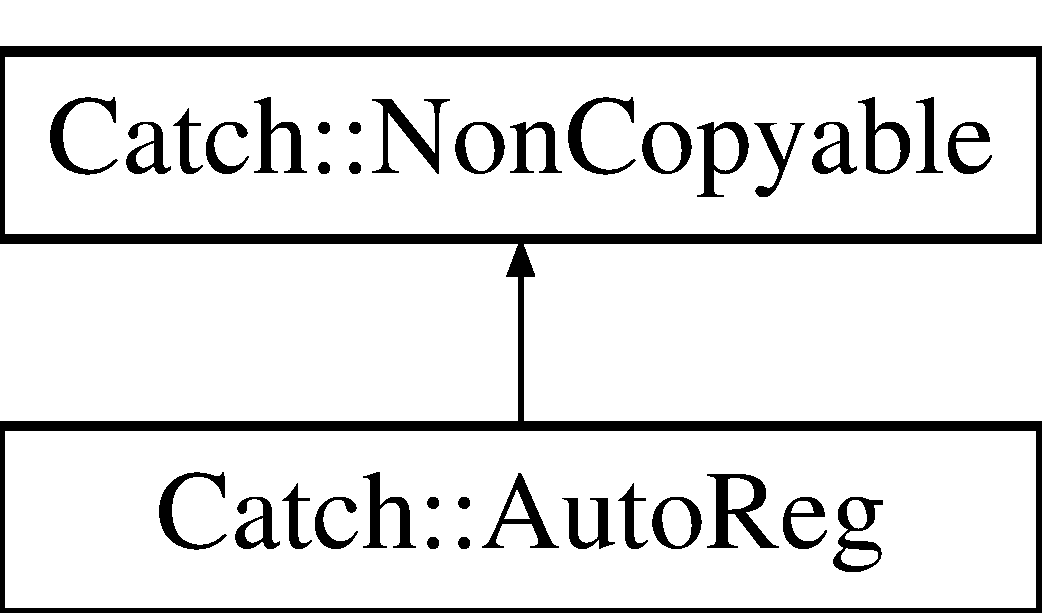
\includegraphics[height=2.000000cm]{struct_catch_1_1_auto_reg}
\end{center}
\end{figure}
\subsection*{Public Member Functions}
\begin{DoxyCompactItemize}
\item 
\mbox{\hyperlink{struct_catch_1_1_auto_reg_a7eba02fb9d80b9896bf5a6517369af28}{Auto\+Reg}} (\mbox{\hyperlink{struct_catch_1_1_i_test_invoker}{I\+Test\+Invoker}} $\ast$invoker, \mbox{\hyperlink{struct_catch_1_1_source_line_info}{Source\+Line\+Info}} const \&line\+Info, \mbox{\hyperlink{class_catch_1_1_string_ref}{String\+Ref}} const \&class\+Or\+Method, \mbox{\hyperlink{struct_catch_1_1_name_and_tags}{Name\+And\+Tags}} const \&name\+And\+Tags) noexcept
\item 
\mbox{\hyperlink{struct_catch_1_1_auto_reg_a3cdb53f1e5ff115310f3372bebe198f1}{$\sim$\+Auto\+Reg}} ()
\end{DoxyCompactItemize}
\subsection*{Additional Inherited Members}


\subsection{Detailed Description}


Definition at line 509 of file catch.\+hpp.



\subsection{Constructor \& Destructor Documentation}
\mbox{\Hypertarget{struct_catch_1_1_auto_reg_a7eba02fb9d80b9896bf5a6517369af28}\label{struct_catch_1_1_auto_reg_a7eba02fb9d80b9896bf5a6517369af28}} 
\index{Catch\+::\+Auto\+Reg@{Catch\+::\+Auto\+Reg}!Auto\+Reg@{Auto\+Reg}}
\index{Auto\+Reg@{Auto\+Reg}!Catch\+::\+Auto\+Reg@{Catch\+::\+Auto\+Reg}}
\subsubsection{\texorpdfstring{Auto\+Reg()}{AutoReg()}}
{\footnotesize\ttfamily Catch\+::\+Auto\+Reg\+::\+Auto\+Reg (\begin{DoxyParamCaption}\item[{\mbox{\hyperlink{struct_catch_1_1_i_test_invoker}{I\+Test\+Invoker}} $\ast$}]{invoker,  }\item[{\mbox{\hyperlink{struct_catch_1_1_source_line_info}{Source\+Line\+Info}} const \&}]{line\+Info,  }\item[{\mbox{\hyperlink{class_catch_1_1_string_ref}{String\+Ref}} const \&}]{class\+Or\+Method,  }\item[{\mbox{\hyperlink{struct_catch_1_1_name_and_tags}{Name\+And\+Tags}} const \&}]{name\+And\+Tags }\end{DoxyParamCaption})\hspace{0.3cm}{\ttfamily [noexcept]}}

\mbox{\Hypertarget{struct_catch_1_1_auto_reg_a3cdb53f1e5ff115310f3372bebe198f1}\label{struct_catch_1_1_auto_reg_a3cdb53f1e5ff115310f3372bebe198f1}} 
\index{Catch\+::\+Auto\+Reg@{Catch\+::\+Auto\+Reg}!````~Auto\+Reg@{$\sim$\+Auto\+Reg}}
\index{````~Auto\+Reg@{$\sim$\+Auto\+Reg}!Catch\+::\+Auto\+Reg@{Catch\+::\+Auto\+Reg}}
\subsubsection{\texorpdfstring{$\sim$\+Auto\+Reg()}{~AutoReg()}}
{\footnotesize\ttfamily Catch\+::\+Auto\+Reg\+::$\sim$\+Auto\+Reg (\begin{DoxyParamCaption}{ }\end{DoxyParamCaption})}



The documentation for this struct was generated from the following file\+:\begin{DoxyCompactItemize}
\item 
D\+:/c++/block\+\_\+matrix-\/master/block\+\_\+matrix-\/master/test/\mbox{\hyperlink{catch_8hpp}{catch.\+hpp}}\end{DoxyCompactItemize}

\hypertarget{class_catch_1_1_benchmark_looper}{}\section{Catch\+:\+:Benchmark\+Looper Class Reference}
\label{class_catch_1_1_benchmark_looper}\index{Catch\+::\+Benchmark\+Looper@{Catch\+::\+Benchmark\+Looper}}


{\ttfamily \#include $<$catch.\+hpp$>$}

\subsection*{Public Member Functions}
\begin{DoxyCompactItemize}
\item 
\mbox{\hyperlink{class_catch_1_1_benchmark_looper_ab9ba6397306a70082f39e63a8a71bde6}{Benchmark\+Looper}} (\mbox{\hyperlink{class_catch_1_1_string_ref}{String\+Ref}} name)
\item 
\mbox{\hyperlink{class_catch_1_1_benchmark_looper_a54da41bada9da038dc05faf41d746765}{operator bool}} ()
\item 
void \mbox{\hyperlink{class_catch_1_1_benchmark_looper_a210552aff5b19408637444d4bb35d59c}{increment}} ()
\item 
void \mbox{\hyperlink{class_catch_1_1_benchmark_looper_a0697d1b266112b110edf2025b82c4e77}{report\+Start}} ()
\item 
auto \mbox{\hyperlink{class_catch_1_1_benchmark_looper_a97bd944521f519b1593a5d1d2f9998fa}{needs\+More\+Iterations}} () -\/$>$ bool
\end{DoxyCompactItemize}


\subsection{Detailed Description}


Definition at line 1857 of file catch.\+hpp.



\subsection{Constructor \& Destructor Documentation}
\mbox{\Hypertarget{class_catch_1_1_benchmark_looper_ab9ba6397306a70082f39e63a8a71bde6}\label{class_catch_1_1_benchmark_looper_ab9ba6397306a70082f39e63a8a71bde6}} 
\index{Catch\+::\+Benchmark\+Looper@{Catch\+::\+Benchmark\+Looper}!Benchmark\+Looper@{Benchmark\+Looper}}
\index{Benchmark\+Looper@{Benchmark\+Looper}!Catch\+::\+Benchmark\+Looper@{Catch\+::\+Benchmark\+Looper}}
\subsubsection{\texorpdfstring{Benchmark\+Looper()}{BenchmarkLooper()}}
{\footnotesize\ttfamily Catch\+::\+Benchmark\+Looper\+::\+Benchmark\+Looper (\begin{DoxyParamCaption}\item[{\mbox{\hyperlink{class_catch_1_1_string_ref}{String\+Ref}}}]{name }\end{DoxyParamCaption})\hspace{0.3cm}{\ttfamily [inline]}}



Definition at line 1868 of file catch.\+hpp.



\subsection{Member Function Documentation}
\mbox{\Hypertarget{class_catch_1_1_benchmark_looper_a210552aff5b19408637444d4bb35d59c}\label{class_catch_1_1_benchmark_looper_a210552aff5b19408637444d4bb35d59c}} 
\index{Catch\+::\+Benchmark\+Looper@{Catch\+::\+Benchmark\+Looper}!increment@{increment}}
\index{increment@{increment}!Catch\+::\+Benchmark\+Looper@{Catch\+::\+Benchmark\+Looper}}
\subsubsection{\texorpdfstring{increment()}{increment()}}
{\footnotesize\ttfamily void Catch\+::\+Benchmark\+Looper\+::increment (\begin{DoxyParamCaption}{ }\end{DoxyParamCaption})\hspace{0.3cm}{\ttfamily [inline]}}



Definition at line 1882 of file catch.\+hpp.

\mbox{\Hypertarget{class_catch_1_1_benchmark_looper_a97bd944521f519b1593a5d1d2f9998fa}\label{class_catch_1_1_benchmark_looper_a97bd944521f519b1593a5d1d2f9998fa}} 
\index{Catch\+::\+Benchmark\+Looper@{Catch\+::\+Benchmark\+Looper}!needs\+More\+Iterations@{needs\+More\+Iterations}}
\index{needs\+More\+Iterations@{needs\+More\+Iterations}!Catch\+::\+Benchmark\+Looper@{Catch\+::\+Benchmark\+Looper}}
\subsubsection{\texorpdfstring{needs\+More\+Iterations()}{needsMoreIterations()}}
{\footnotesize\ttfamily auto Catch\+::\+Benchmark\+Looper\+::needs\+More\+Iterations (\begin{DoxyParamCaption}{ }\end{DoxyParamCaption}) -\/$>$  bool}

\mbox{\Hypertarget{class_catch_1_1_benchmark_looper_a54da41bada9da038dc05faf41d746765}\label{class_catch_1_1_benchmark_looper_a54da41bada9da038dc05faf41d746765}} 
\index{Catch\+::\+Benchmark\+Looper@{Catch\+::\+Benchmark\+Looper}!operator bool@{operator bool}}
\index{operator bool@{operator bool}!Catch\+::\+Benchmark\+Looper@{Catch\+::\+Benchmark\+Looper}}
\subsubsection{\texorpdfstring{operator bool()}{operator bool()}}
{\footnotesize\ttfamily Catch\+::\+Benchmark\+Looper\+::operator bool (\begin{DoxyParamCaption}{ }\end{DoxyParamCaption})\hspace{0.3cm}{\ttfamily [inline]}, {\ttfamily [explicit]}}



Definition at line 1876 of file catch.\+hpp.

\mbox{\Hypertarget{class_catch_1_1_benchmark_looper_a0697d1b266112b110edf2025b82c4e77}\label{class_catch_1_1_benchmark_looper_a0697d1b266112b110edf2025b82c4e77}} 
\index{Catch\+::\+Benchmark\+Looper@{Catch\+::\+Benchmark\+Looper}!report\+Start@{report\+Start}}
\index{report\+Start@{report\+Start}!Catch\+::\+Benchmark\+Looper@{Catch\+::\+Benchmark\+Looper}}
\subsubsection{\texorpdfstring{report\+Start()}{reportStart()}}
{\footnotesize\ttfamily void Catch\+::\+Benchmark\+Looper\+::report\+Start (\begin{DoxyParamCaption}{ }\end{DoxyParamCaption})}



The documentation for this class was generated from the following file\+:\begin{DoxyCompactItemize}
\item 
D\+:/c++/block\+\_\+matrix-\/master/block\+\_\+matrix-\/master/test/\mbox{\hyperlink{catch_8hpp}{catch.\+hpp}}\end{DoxyCompactItemize}

\hypertarget{class_catch_1_1_binary_expr}{}\section{Catch\+:\+:Binary\+Expr$<$ LhsT, RhsT $>$ Class Template Reference}
\label{class_catch_1_1_binary_expr}\index{Catch\+::\+Binary\+Expr$<$ Lhs\+T, Rhs\+T $>$@{Catch\+::\+Binary\+Expr$<$ Lhs\+T, Rhs\+T $>$}}


{\ttfamily \#include $<$catch.\+hpp$>$}

Inheritance diagram for Catch\+:\+:Binary\+Expr$<$ LhsT, RhsT $>$\+:\begin{figure}[H]
\begin{center}
\leavevmode
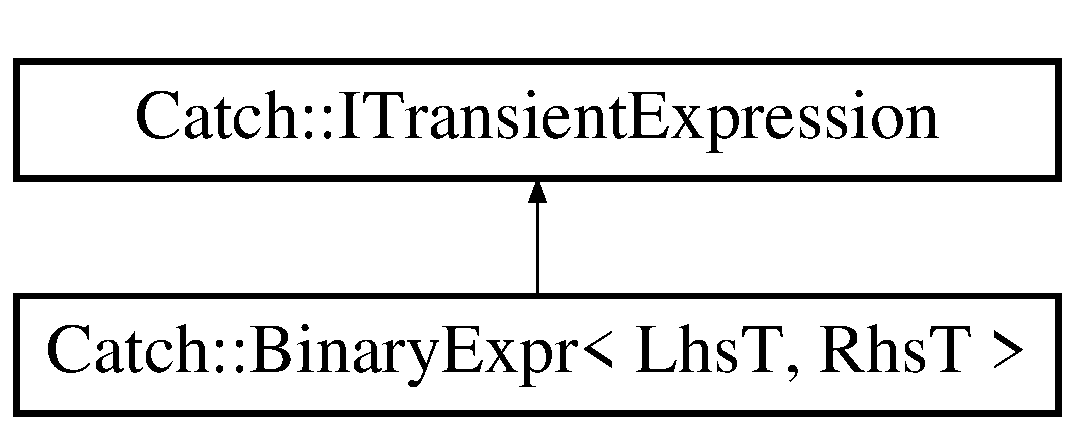
\includegraphics[height=2.000000cm]{class_catch_1_1_binary_expr}
\end{center}
\end{figure}
\subsection*{Public Member Functions}
\begin{DoxyCompactItemize}
\item 
\mbox{\hyperlink{class_catch_1_1_binary_expr_a657d66346aef97a760c22776fe6008b6}{Binary\+Expr}} (bool comparison\+Result, LhsT lhs, \mbox{\hyperlink{class_catch_1_1_string_ref}{String\+Ref}} op, RhsT rhs)
\end{DoxyCompactItemize}
\subsection*{Additional Inherited Members}


\subsection{Detailed Description}
\subsubsection*{template$<$typename LhsT, typename RhsT$>$\newline
class Catch\+::\+Binary\+Expr$<$ Lhs\+T, Rhs\+T $>$}



Definition at line 1277 of file catch.\+hpp.



\subsection{Constructor \& Destructor Documentation}
\mbox{\Hypertarget{class_catch_1_1_binary_expr_a657d66346aef97a760c22776fe6008b6}\label{class_catch_1_1_binary_expr_a657d66346aef97a760c22776fe6008b6}} 
\index{Catch\+::\+Binary\+Expr@{Catch\+::\+Binary\+Expr}!Binary\+Expr@{Binary\+Expr}}
\index{Binary\+Expr@{Binary\+Expr}!Catch\+::\+Binary\+Expr@{Catch\+::\+Binary\+Expr}}
\subsubsection{\texorpdfstring{Binary\+Expr()}{BinaryExpr()}}
{\footnotesize\ttfamily template$<$typename LhsT , typename RhsT $>$ \\
\mbox{\hyperlink{class_catch_1_1_binary_expr}{Catch\+::\+Binary\+Expr}}$<$ LhsT, RhsT $>$\+::\mbox{\hyperlink{class_catch_1_1_binary_expr}{Binary\+Expr}} (\begin{DoxyParamCaption}\item[{bool}]{comparison\+Result,  }\item[{LhsT}]{lhs,  }\item[{\mbox{\hyperlink{class_catch_1_1_string_ref}{String\+Ref}}}]{op,  }\item[{RhsT}]{rhs }\end{DoxyParamCaption})\hspace{0.3cm}{\ttfamily [inline]}}



Definition at line 1288 of file catch.\+hpp.



The documentation for this class was generated from the following file\+:\begin{DoxyCompactItemize}
\item 
D\+:/c++/block\+\_\+matrix-\/master/block\+\_\+matrix-\/master/test/\mbox{\hyperlink{catch_8hpp}{catch.\+hpp}}\end{DoxyCompactItemize}

\hypertarget{classbmx_1_1block__matrix}{}\section{bmx\+:\+:block\+\_\+matrix$<$ Type $>$ Class Template Reference}
\label{classbmx_1_1block__matrix}\index{bmx\+::block\+\_\+matrix$<$ Type $>$@{bmx\+::block\+\_\+matrix$<$ Type $>$}}


{\ttfamily \#include $<$block\+\_\+matrix.\+hpp$>$}

\subsection*{Public Member Functions}
\begin{DoxyCompactItemize}
\item 
\mbox{\hyperlink{classbmx_1_1block__matrix_a04826c7a53ad8da87b0e9eede8af679a}{block\+\_\+matrix}} ()
\item 
\mbox{\hyperlink{classbmx_1_1block__matrix_a8356cfaa8cc00082ec82070f4143b6fa}{block\+\_\+matrix}} (const std\+::size\+\_\+t \+\_\+size\+\_\+one, const std\+::size\+\_\+t \+\_\+size\+\_\+two)
\item 
std\+::size\+\_\+t \mbox{\hyperlink{classbmx_1_1block__matrix_afe5002a570f6c7ae455add2ab3ad3c87}{size}} ()
\item 
void \mbox{\hyperlink{classbmx_1_1block__matrix_a3708a438e204c7479da201365e088212}{set\+\_\+block\+\_\+one}} (std\+::size\+\_\+t size\+\_\+one, Type element)
\item 
void \mbox{\hyperlink{classbmx_1_1block__matrix_a1233de84f6828b5b3dd80af76c0688bd}{set\+\_\+block\+\_\+two}} (std\+::size\+\_\+t size\+\_\+two, Type element)
\item 
void \mbox{\hyperlink{classbmx_1_1block__matrix_a010884e7b07582cd28e1de9d58521b62}{write\+\_\+out\+\_\+matrix1}} ()
\item 
void \mbox{\hyperlink{classbmx_1_1block__matrix_a5e758f4af743778dedce4ce05f95a14a}{write\+\_\+out\+\_\+matrix2}} ()
\item 
Type \mbox{\hyperlink{classbmx_1_1block__matrix_ab8c567ac66dabb15646b951fe55f30b6}{get\+\_\+block\+\_\+one\+\_\+values}} (const int i, const int j)
\item 
Type \mbox{\hyperlink{classbmx_1_1block__matrix_a4737a14c292308edbf16d71b3b6240a2}{get\+\_\+block\+\_\+two\+\_\+values}} (const int i, const int j)
\item 
void \mbox{\hyperlink{classbmx_1_1block__matrix_aa6200f28e371684979facaf7494bd755}{sum}} (\mbox{\hyperlink{classbmx_1_1block__matrix}{bmx\+::block\+\_\+matrix}}$<$ Type $>$ \&b)
\item 
void \mbox{\hyperlink{classbmx_1_1block__matrix_a5a6c1c462b530c2dcf8bc24a0e6dc85c}{multiplication}} (\mbox{\hyperlink{classbmx_1_1block__matrix}{bmx\+::block\+\_\+matrix}}$<$ Type $>$ \&b)
\item 
void \mbox{\hyperlink{classbmx_1_1block__matrix_a6e7219a6e1c65c1ddcc1a64cdab56223}{print}} ()
\item 
int \mbox{\hyperlink{classbmx_1_1block__matrix_a3a4e7a297cb5e09564f0a3b74cbdfaec}{get}} (const int x, const int y) const
\end{DoxyCompactItemize}


\subsection{Detailed Description}
\subsubsection*{template$<$class Type = int$>$\newline
class bmx\+::block\+\_\+matrix$<$ Type $>$}



Definition at line 12 of file block\+\_\+matrix.\+hpp.



\subsection{Constructor \& Destructor Documentation}
\mbox{\Hypertarget{classbmx_1_1block__matrix_a04826c7a53ad8da87b0e9eede8af679a}\label{classbmx_1_1block__matrix_a04826c7a53ad8da87b0e9eede8af679a}} 
\index{bmx\+::block\+\_\+matrix@{bmx\+::block\+\_\+matrix}!block\+\_\+matrix@{block\+\_\+matrix}}
\index{block\+\_\+matrix@{block\+\_\+matrix}!bmx\+::block\+\_\+matrix@{bmx\+::block\+\_\+matrix}}
\subsubsection{\texorpdfstring{block\+\_\+matrix()}{block\_matrix()}\hspace{0.1cm}{\footnotesize\ttfamily [1/2]}}
{\footnotesize\ttfamily template$<$class Type = int$>$ \\
\mbox{\hyperlink{classbmx_1_1block__matrix}{bmx\+::block\+\_\+matrix}}$<$ Type $>$\+::\mbox{\hyperlink{classbmx_1_1block__matrix}{block\+\_\+matrix}} (\begin{DoxyParamCaption}{ }\end{DoxyParamCaption})\hspace{0.3cm}{\ttfamily [inline]}}



Definition at line 20 of file block\+\_\+matrix.\+hpp.

\mbox{\Hypertarget{classbmx_1_1block__matrix_a8356cfaa8cc00082ec82070f4143b6fa}\label{classbmx_1_1block__matrix_a8356cfaa8cc00082ec82070f4143b6fa}} 
\index{bmx\+::block\+\_\+matrix@{bmx\+::block\+\_\+matrix}!block\+\_\+matrix@{block\+\_\+matrix}}
\index{block\+\_\+matrix@{block\+\_\+matrix}!bmx\+::block\+\_\+matrix@{bmx\+::block\+\_\+matrix}}
\subsubsection{\texorpdfstring{block\+\_\+matrix()}{block\_matrix()}\hspace{0.1cm}{\footnotesize\ttfamily [2/2]}}
{\footnotesize\ttfamily template$<$class Type = int$>$ \\
\mbox{\hyperlink{classbmx_1_1block__matrix}{bmx\+::block\+\_\+matrix}}$<$ Type $>$\+::\mbox{\hyperlink{classbmx_1_1block__matrix}{block\+\_\+matrix}} (\begin{DoxyParamCaption}\item[{const std\+::size\+\_\+t}]{\+\_\+size\+\_\+one,  }\item[{const std\+::size\+\_\+t}]{\+\_\+size\+\_\+two }\end{DoxyParamCaption})\hspace{0.3cm}{\ttfamily [inline]}}



Definition at line 22 of file block\+\_\+matrix.\+hpp.



\subsection{Member Function Documentation}
\mbox{\Hypertarget{classbmx_1_1block__matrix_a3a4e7a297cb5e09564f0a3b74cbdfaec}\label{classbmx_1_1block__matrix_a3a4e7a297cb5e09564f0a3b74cbdfaec}} 
\index{bmx\+::block\+\_\+matrix@{bmx\+::block\+\_\+matrix}!get@{get}}
\index{get@{get}!bmx\+::block\+\_\+matrix@{bmx\+::block\+\_\+matrix}}
\subsubsection{\texorpdfstring{get()}{get()}}
{\footnotesize\ttfamily template$<$class Type = int$>$ \\
int \mbox{\hyperlink{classbmx_1_1block__matrix}{bmx\+::block\+\_\+matrix}}$<$ Type $>$\+::get (\begin{DoxyParamCaption}\item[{const int}]{x,  }\item[{const int}]{y }\end{DoxyParamCaption}) const\hspace{0.3cm}{\ttfamily [inline]}}



Definition at line 190 of file block\+\_\+matrix.\+hpp.

\mbox{\Hypertarget{classbmx_1_1block__matrix_ab8c567ac66dabb15646b951fe55f30b6}\label{classbmx_1_1block__matrix_ab8c567ac66dabb15646b951fe55f30b6}} 
\index{bmx\+::block\+\_\+matrix@{bmx\+::block\+\_\+matrix}!get\+\_\+block\+\_\+one\+\_\+values@{get\+\_\+block\+\_\+one\+\_\+values}}
\index{get\+\_\+block\+\_\+one\+\_\+values@{get\+\_\+block\+\_\+one\+\_\+values}!bmx\+::block\+\_\+matrix@{bmx\+::block\+\_\+matrix}}
\subsubsection{\texorpdfstring{get\+\_\+block\+\_\+one\+\_\+values()}{get\_block\_one\_values()}}
{\footnotesize\ttfamily template$<$class Type = int$>$ \\
Type \mbox{\hyperlink{classbmx_1_1block__matrix}{bmx\+::block\+\_\+matrix}}$<$ Type $>$\+::get\+\_\+block\+\_\+one\+\_\+values (\begin{DoxyParamCaption}\item[{const int}]{i,  }\item[{const int}]{j }\end{DoxyParamCaption})\hspace{0.3cm}{\ttfamily [inline]}}



Definition at line 91 of file block\+\_\+matrix.\+hpp.

\mbox{\Hypertarget{classbmx_1_1block__matrix_a4737a14c292308edbf16d71b3b6240a2}\label{classbmx_1_1block__matrix_a4737a14c292308edbf16d71b3b6240a2}} 
\index{bmx\+::block\+\_\+matrix@{bmx\+::block\+\_\+matrix}!get\+\_\+block\+\_\+two\+\_\+values@{get\+\_\+block\+\_\+two\+\_\+values}}
\index{get\+\_\+block\+\_\+two\+\_\+values@{get\+\_\+block\+\_\+two\+\_\+values}!bmx\+::block\+\_\+matrix@{bmx\+::block\+\_\+matrix}}
\subsubsection{\texorpdfstring{get\+\_\+block\+\_\+two\+\_\+values()}{get\_block\_two\_values()}}
{\footnotesize\ttfamily template$<$class Type = int$>$ \\
Type \mbox{\hyperlink{classbmx_1_1block__matrix}{bmx\+::block\+\_\+matrix}}$<$ Type $>$\+::get\+\_\+block\+\_\+two\+\_\+values (\begin{DoxyParamCaption}\item[{const int}]{i,  }\item[{const int}]{j }\end{DoxyParamCaption})\hspace{0.3cm}{\ttfamily [inline]}}



Definition at line 102 of file block\+\_\+matrix.\+hpp.

\mbox{\Hypertarget{classbmx_1_1block__matrix_a5a6c1c462b530c2dcf8bc24a0e6dc85c}\label{classbmx_1_1block__matrix_a5a6c1c462b530c2dcf8bc24a0e6dc85c}} 
\index{bmx\+::block\+\_\+matrix@{bmx\+::block\+\_\+matrix}!multiplication@{multiplication}}
\index{multiplication@{multiplication}!bmx\+::block\+\_\+matrix@{bmx\+::block\+\_\+matrix}}
\subsubsection{\texorpdfstring{multiplication()}{multiplication()}}
{\footnotesize\ttfamily template$<$class Type = int$>$ \\
void \mbox{\hyperlink{classbmx_1_1block__matrix}{bmx\+::block\+\_\+matrix}}$<$ Type $>$\+::multiplication (\begin{DoxyParamCaption}\item[{\mbox{\hyperlink{classbmx_1_1block__matrix}{bmx\+::block\+\_\+matrix}}$<$ Type $>$ \&}]{b }\end{DoxyParamCaption})\hspace{0.3cm}{\ttfamily [inline]}}



Definition at line 132 of file block\+\_\+matrix.\+hpp.

\mbox{\Hypertarget{classbmx_1_1block__matrix_a6e7219a6e1c65c1ddcc1a64cdab56223}\label{classbmx_1_1block__matrix_a6e7219a6e1c65c1ddcc1a64cdab56223}} 
\index{bmx\+::block\+\_\+matrix@{bmx\+::block\+\_\+matrix}!print@{print}}
\index{print@{print}!bmx\+::block\+\_\+matrix@{bmx\+::block\+\_\+matrix}}
\subsubsection{\texorpdfstring{print()}{print()}}
{\footnotesize\ttfamily template$<$class Type = int$>$ \\
void \mbox{\hyperlink{classbmx_1_1block__matrix}{bmx\+::block\+\_\+matrix}}$<$ Type $>$\+::print (\begin{DoxyParamCaption}{ }\end{DoxyParamCaption})\hspace{0.3cm}{\ttfamily [inline]}}



Definition at line 151 of file block\+\_\+matrix.\+hpp.

\mbox{\Hypertarget{classbmx_1_1block__matrix_a3708a438e204c7479da201365e088212}\label{classbmx_1_1block__matrix_a3708a438e204c7479da201365e088212}} 
\index{bmx\+::block\+\_\+matrix@{bmx\+::block\+\_\+matrix}!set\+\_\+block\+\_\+one@{set\+\_\+block\+\_\+one}}
\index{set\+\_\+block\+\_\+one@{set\+\_\+block\+\_\+one}!bmx\+::block\+\_\+matrix@{bmx\+::block\+\_\+matrix}}
\subsubsection{\texorpdfstring{set\+\_\+block\+\_\+one()}{set\_block\_one()}}
{\footnotesize\ttfamily template$<$class Type = int$>$ \\
void \mbox{\hyperlink{classbmx_1_1block__matrix}{bmx\+::block\+\_\+matrix}}$<$ Type $>$\+::set\+\_\+block\+\_\+one (\begin{DoxyParamCaption}\item[{std\+::size\+\_\+t}]{size\+\_\+one,  }\item[{Type}]{element }\end{DoxyParamCaption})\hspace{0.3cm}{\ttfamily [inline]}}



Definition at line 37 of file block\+\_\+matrix.\+hpp.

\mbox{\Hypertarget{classbmx_1_1block__matrix_a1233de84f6828b5b3dd80af76c0688bd}\label{classbmx_1_1block__matrix_a1233de84f6828b5b3dd80af76c0688bd}} 
\index{bmx\+::block\+\_\+matrix@{bmx\+::block\+\_\+matrix}!set\+\_\+block\+\_\+two@{set\+\_\+block\+\_\+two}}
\index{set\+\_\+block\+\_\+two@{set\+\_\+block\+\_\+two}!bmx\+::block\+\_\+matrix@{bmx\+::block\+\_\+matrix}}
\subsubsection{\texorpdfstring{set\+\_\+block\+\_\+two()}{set\_block\_two()}}
{\footnotesize\ttfamily template$<$class Type = int$>$ \\
void \mbox{\hyperlink{classbmx_1_1block__matrix}{bmx\+::block\+\_\+matrix}}$<$ Type $>$\+::set\+\_\+block\+\_\+two (\begin{DoxyParamCaption}\item[{std\+::size\+\_\+t}]{size\+\_\+two,  }\item[{Type}]{element }\end{DoxyParamCaption})\hspace{0.3cm}{\ttfamily [inline]}}



Definition at line 54 of file block\+\_\+matrix.\+hpp.

\mbox{\Hypertarget{classbmx_1_1block__matrix_afe5002a570f6c7ae455add2ab3ad3c87}\label{classbmx_1_1block__matrix_afe5002a570f6c7ae455add2ab3ad3c87}} 
\index{bmx\+::block\+\_\+matrix@{bmx\+::block\+\_\+matrix}!size@{size}}
\index{size@{size}!bmx\+::block\+\_\+matrix@{bmx\+::block\+\_\+matrix}}
\subsubsection{\texorpdfstring{size()}{size()}}
{\footnotesize\ttfamily template$<$class Type = int$>$ \\
std\+::size\+\_\+t \mbox{\hyperlink{classbmx_1_1block__matrix}{bmx\+::block\+\_\+matrix}}$<$ Type $>$\+::size (\begin{DoxyParamCaption}{ }\end{DoxyParamCaption})\hspace{0.3cm}{\ttfamily [inline]}}



Definition at line 32 of file block\+\_\+matrix.\+hpp.

\mbox{\Hypertarget{classbmx_1_1block__matrix_aa6200f28e371684979facaf7494bd755}\label{classbmx_1_1block__matrix_aa6200f28e371684979facaf7494bd755}} 
\index{bmx\+::block\+\_\+matrix@{bmx\+::block\+\_\+matrix}!sum@{sum}}
\index{sum@{sum}!bmx\+::block\+\_\+matrix@{bmx\+::block\+\_\+matrix}}
\subsubsection{\texorpdfstring{sum()}{sum()}}
{\footnotesize\ttfamily template$<$class Type = int$>$ \\
void \mbox{\hyperlink{classbmx_1_1block__matrix}{bmx\+::block\+\_\+matrix}}$<$ Type $>$\+::sum (\begin{DoxyParamCaption}\item[{\mbox{\hyperlink{classbmx_1_1block__matrix}{bmx\+::block\+\_\+matrix}}$<$ Type $>$ \&}]{b }\end{DoxyParamCaption})\hspace{0.3cm}{\ttfamily [inline]}}



Definition at line 113 of file block\+\_\+matrix.\+hpp.

\mbox{\Hypertarget{classbmx_1_1block__matrix_a010884e7b07582cd28e1de9d58521b62}\label{classbmx_1_1block__matrix_a010884e7b07582cd28e1de9d58521b62}} 
\index{bmx\+::block\+\_\+matrix@{bmx\+::block\+\_\+matrix}!write\+\_\+out\+\_\+matrix1@{write\+\_\+out\+\_\+matrix1}}
\index{write\+\_\+out\+\_\+matrix1@{write\+\_\+out\+\_\+matrix1}!bmx\+::block\+\_\+matrix@{bmx\+::block\+\_\+matrix}}
\subsubsection{\texorpdfstring{write\+\_\+out\+\_\+matrix1()}{write\_out\_matrix1()}}
{\footnotesize\ttfamily template$<$class Type = int$>$ \\
void \mbox{\hyperlink{classbmx_1_1block__matrix}{bmx\+::block\+\_\+matrix}}$<$ Type $>$\+::write\+\_\+out\+\_\+matrix1 (\begin{DoxyParamCaption}{ }\end{DoxyParamCaption})\hspace{0.3cm}{\ttfamily [inline]}}



Definition at line 70 of file block\+\_\+matrix.\+hpp.

\mbox{\Hypertarget{classbmx_1_1block__matrix_a5e758f4af743778dedce4ce05f95a14a}\label{classbmx_1_1block__matrix_a5e758f4af743778dedce4ce05f95a14a}} 
\index{bmx\+::block\+\_\+matrix@{bmx\+::block\+\_\+matrix}!write\+\_\+out\+\_\+matrix2@{write\+\_\+out\+\_\+matrix2}}
\index{write\+\_\+out\+\_\+matrix2@{write\+\_\+out\+\_\+matrix2}!bmx\+::block\+\_\+matrix@{bmx\+::block\+\_\+matrix}}
\subsubsection{\texorpdfstring{write\+\_\+out\+\_\+matrix2()}{write\_out\_matrix2()}}
{\footnotesize\ttfamily template$<$class Type = int$>$ \\
void \mbox{\hyperlink{classbmx_1_1block__matrix}{bmx\+::block\+\_\+matrix}}$<$ Type $>$\+::write\+\_\+out\+\_\+matrix2 (\begin{DoxyParamCaption}{ }\end{DoxyParamCaption})\hspace{0.3cm}{\ttfamily [inline]}}



Definition at line 81 of file block\+\_\+matrix.\+hpp.



The documentation for this class was generated from the following file\+:\begin{DoxyCompactItemize}
\item 
D\+:/c++/block\+\_\+matrix-\/master/block\+\_\+matrix-\/master/test/include/\mbox{\hyperlink{test_2include_2block__matrix_8hpp}{block\+\_\+matrix.\+hpp}}\end{DoxyCompactItemize}

\hypertarget{struct_catch_1_1_matchers_1_1_std_string_1_1_cased_string}{}\section{Catch\+:\+:Matchers\+:\+:Std\+String\+:\+:Cased\+String Struct Reference}
\label{struct_catch_1_1_matchers_1_1_std_string_1_1_cased_string}\index{Catch\+::\+Matchers\+::\+Std\+String\+::\+Cased\+String@{Catch\+::\+Matchers\+::\+Std\+String\+::\+Cased\+String}}


{\ttfamily \#include $<$catch.\+hpp$>$}

\subsection*{Public Member Functions}
\begin{DoxyCompactItemize}
\item 
\mbox{\hyperlink{struct_catch_1_1_matchers_1_1_std_string_1_1_cased_string_aa88bbc5acd2bff22351d8d4b1816b561}{Cased\+String}} (std\+::string const \&str, \mbox{\hyperlink{struct_catch_1_1_case_sensitive_aad49d3aee2d97066642fffa919685c6a}{Case\+Sensitive\+::\+Choice}} case\+Sensitivity)
\item 
std\+::string \mbox{\hyperlink{struct_catch_1_1_matchers_1_1_std_string_1_1_cased_string_a77639b1165c01f424ee0e96f53335010}{adjust\+String}} (std\+::string const \&str) const
\item 
std\+::string \mbox{\hyperlink{struct_catch_1_1_matchers_1_1_std_string_1_1_cased_string_a9759155344d696b2476d764a1d95fcc9}{case\+Sensitivity\+Suffix}} () const
\end{DoxyCompactItemize}
\subsection*{Public Attributes}
\begin{DoxyCompactItemize}
\item 
\mbox{\hyperlink{struct_catch_1_1_case_sensitive_aad49d3aee2d97066642fffa919685c6a}{Case\+Sensitive\+::\+Choice}} \mbox{\hyperlink{struct_catch_1_1_matchers_1_1_std_string_1_1_cased_string_ae1c2864c986941536a6e94cca0528f92}{m\+\_\+case\+Sensitivity}}
\item 
std\+::string \mbox{\hyperlink{struct_catch_1_1_matchers_1_1_std_string_1_1_cased_string_ad05dbc99aba3c3c386d6b856b213f911}{m\+\_\+str}}
\end{DoxyCompactItemize}


\subsection{Detailed Description}


Definition at line 2369 of file catch.\+hpp.



\subsection{Constructor \& Destructor Documentation}
\mbox{\Hypertarget{struct_catch_1_1_matchers_1_1_std_string_1_1_cased_string_aa88bbc5acd2bff22351d8d4b1816b561}\label{struct_catch_1_1_matchers_1_1_std_string_1_1_cased_string_aa88bbc5acd2bff22351d8d4b1816b561}} 
\index{Catch\+::\+Matchers\+::\+Std\+String\+::\+Cased\+String@{Catch\+::\+Matchers\+::\+Std\+String\+::\+Cased\+String}!Cased\+String@{Cased\+String}}
\index{Cased\+String@{Cased\+String}!Catch\+::\+Matchers\+::\+Std\+String\+::\+Cased\+String@{Catch\+::\+Matchers\+::\+Std\+String\+::\+Cased\+String}}
\subsubsection{\texorpdfstring{Cased\+String()}{CasedString()}}
{\footnotesize\ttfamily Catch\+::\+Matchers\+::\+Std\+String\+::\+Cased\+String\+::\+Cased\+String (\begin{DoxyParamCaption}\item[{std\+::string const \&}]{str,  }\item[{\mbox{\hyperlink{struct_catch_1_1_case_sensitive_aad49d3aee2d97066642fffa919685c6a}{Case\+Sensitive\+::\+Choice}}}]{case\+Sensitivity }\end{DoxyParamCaption})}



\subsection{Member Function Documentation}
\mbox{\Hypertarget{struct_catch_1_1_matchers_1_1_std_string_1_1_cased_string_a77639b1165c01f424ee0e96f53335010}\label{struct_catch_1_1_matchers_1_1_std_string_1_1_cased_string_a77639b1165c01f424ee0e96f53335010}} 
\index{Catch\+::\+Matchers\+::\+Std\+String\+::\+Cased\+String@{Catch\+::\+Matchers\+::\+Std\+String\+::\+Cased\+String}!adjust\+String@{adjust\+String}}
\index{adjust\+String@{adjust\+String}!Catch\+::\+Matchers\+::\+Std\+String\+::\+Cased\+String@{Catch\+::\+Matchers\+::\+Std\+String\+::\+Cased\+String}}
\subsubsection{\texorpdfstring{adjust\+String()}{adjustString()}}
{\footnotesize\ttfamily std\+::string Catch\+::\+Matchers\+::\+Std\+String\+::\+Cased\+String\+::adjust\+String (\begin{DoxyParamCaption}\item[{std\+::string const \&}]{str }\end{DoxyParamCaption}) const}

\mbox{\Hypertarget{struct_catch_1_1_matchers_1_1_std_string_1_1_cased_string_a9759155344d696b2476d764a1d95fcc9}\label{struct_catch_1_1_matchers_1_1_std_string_1_1_cased_string_a9759155344d696b2476d764a1d95fcc9}} 
\index{Catch\+::\+Matchers\+::\+Std\+String\+::\+Cased\+String@{Catch\+::\+Matchers\+::\+Std\+String\+::\+Cased\+String}!case\+Sensitivity\+Suffix@{case\+Sensitivity\+Suffix}}
\index{case\+Sensitivity\+Suffix@{case\+Sensitivity\+Suffix}!Catch\+::\+Matchers\+::\+Std\+String\+::\+Cased\+String@{Catch\+::\+Matchers\+::\+Std\+String\+::\+Cased\+String}}
\subsubsection{\texorpdfstring{case\+Sensitivity\+Suffix()}{caseSensitivitySuffix()}}
{\footnotesize\ttfamily std\+::string Catch\+::\+Matchers\+::\+Std\+String\+::\+Cased\+String\+::case\+Sensitivity\+Suffix (\begin{DoxyParamCaption}{ }\end{DoxyParamCaption}) const}



\subsection{Member Data Documentation}
\mbox{\Hypertarget{struct_catch_1_1_matchers_1_1_std_string_1_1_cased_string_ae1c2864c986941536a6e94cca0528f92}\label{struct_catch_1_1_matchers_1_1_std_string_1_1_cased_string_ae1c2864c986941536a6e94cca0528f92}} 
\index{Catch\+::\+Matchers\+::\+Std\+String\+::\+Cased\+String@{Catch\+::\+Matchers\+::\+Std\+String\+::\+Cased\+String}!m\+\_\+case\+Sensitivity@{m\+\_\+case\+Sensitivity}}
\index{m\+\_\+case\+Sensitivity@{m\+\_\+case\+Sensitivity}!Catch\+::\+Matchers\+::\+Std\+String\+::\+Cased\+String@{Catch\+::\+Matchers\+::\+Std\+String\+::\+Cased\+String}}
\subsubsection{\texorpdfstring{m\+\_\+case\+Sensitivity}{m\_caseSensitivity}}
{\footnotesize\ttfamily \mbox{\hyperlink{struct_catch_1_1_case_sensitive_aad49d3aee2d97066642fffa919685c6a}{Case\+Sensitive\+::\+Choice}} Catch\+::\+Matchers\+::\+Std\+String\+::\+Cased\+String\+::m\+\_\+case\+Sensitivity}



Definition at line 2375 of file catch.\+hpp.

\mbox{\Hypertarget{struct_catch_1_1_matchers_1_1_std_string_1_1_cased_string_ad05dbc99aba3c3c386d6b856b213f911}\label{struct_catch_1_1_matchers_1_1_std_string_1_1_cased_string_ad05dbc99aba3c3c386d6b856b213f911}} 
\index{Catch\+::\+Matchers\+::\+Std\+String\+::\+Cased\+String@{Catch\+::\+Matchers\+::\+Std\+String\+::\+Cased\+String}!m\+\_\+str@{m\+\_\+str}}
\index{m\+\_\+str@{m\+\_\+str}!Catch\+::\+Matchers\+::\+Std\+String\+::\+Cased\+String@{Catch\+::\+Matchers\+::\+Std\+String\+::\+Cased\+String}}
\subsubsection{\texorpdfstring{m\+\_\+str}{m\_str}}
{\footnotesize\ttfamily std\+::string Catch\+::\+Matchers\+::\+Std\+String\+::\+Cased\+String\+::m\+\_\+str}



Definition at line 2376 of file catch.\+hpp.



The documentation for this struct was generated from the following file\+:\begin{DoxyCompactItemize}
\item 
D\+:/c++/block\+\_\+matrix-\/master/block\+\_\+matrix-\/master/test/\mbox{\hyperlink{catch_8hpp}{catch.\+hpp}}\end{DoxyCompactItemize}

\hypertarget{struct_catch_1_1_case_sensitive}{}\section{Catch\+:\+:Case\+Sensitive Struct Reference}
\label{struct_catch_1_1_case_sensitive}\index{Catch\+::\+Case\+Sensitive@{Catch\+::\+Case\+Sensitive}}


{\ttfamily \#include $<$catch.\+hpp$>$}

\subsection*{Public Types}
\begin{DoxyCompactItemize}
\item 
enum \mbox{\hyperlink{struct_catch_1_1_case_sensitive_aad49d3aee2d97066642fffa919685c6a}{Choice}} \{ \mbox{\hyperlink{struct_catch_1_1_case_sensitive_aad49d3aee2d97066642fffa919685c6aa7c5550b69ec3c502e6f609b67f9613c6}{Yes}}, 
\mbox{\hyperlink{struct_catch_1_1_case_sensitive_aad49d3aee2d97066642fffa919685c6aa4ffff8d29b481f0116abc37228cd53f6}{No}}
 \}
\end{DoxyCompactItemize}


\subsection{Detailed Description}


Definition at line 256 of file catch.\+hpp.



\subsection{Member Enumeration Documentation}
\mbox{\Hypertarget{struct_catch_1_1_case_sensitive_aad49d3aee2d97066642fffa919685c6a}\label{struct_catch_1_1_case_sensitive_aad49d3aee2d97066642fffa919685c6a}} 
\index{Catch\+::\+Case\+Sensitive@{Catch\+::\+Case\+Sensitive}!Choice@{Choice}}
\index{Choice@{Choice}!Catch\+::\+Case\+Sensitive@{Catch\+::\+Case\+Sensitive}}
\subsubsection{\texorpdfstring{Choice}{Choice}}
{\footnotesize\ttfamily enum \mbox{\hyperlink{struct_catch_1_1_case_sensitive_aad49d3aee2d97066642fffa919685c6a}{Catch\+::\+Case\+Sensitive\+::\+Choice}}}

\begin{DoxyEnumFields}{Enumerator}
\raisebox{\heightof{T}}[0pt][0pt]{\index{Yes@{Yes}!Catch\+::\+Case\+Sensitive@{Catch\+::\+Case\+Sensitive}}\index{Catch\+::\+Case\+Sensitive@{Catch\+::\+Case\+Sensitive}!Yes@{Yes}}}\mbox{\Hypertarget{struct_catch_1_1_case_sensitive_aad49d3aee2d97066642fffa919685c6aa7c5550b69ec3c502e6f609b67f9613c6}\label{struct_catch_1_1_case_sensitive_aad49d3aee2d97066642fffa919685c6aa7c5550b69ec3c502e6f609b67f9613c6}} 
Yes&\\
\hline

\raisebox{\heightof{T}}[0pt][0pt]{\index{No@{No}!Catch\+::\+Case\+Sensitive@{Catch\+::\+Case\+Sensitive}}\index{Catch\+::\+Case\+Sensitive@{Catch\+::\+Case\+Sensitive}!No@{No}}}\mbox{\Hypertarget{struct_catch_1_1_case_sensitive_aad49d3aee2d97066642fffa919685c6aa4ffff8d29b481f0116abc37228cd53f6}\label{struct_catch_1_1_case_sensitive_aad49d3aee2d97066642fffa919685c6aa4ffff8d29b481f0116abc37228cd53f6}} 
No&\\
\hline

\end{DoxyEnumFields}


Definition at line 256 of file catch.\+hpp.



The documentation for this struct was generated from the following file\+:\begin{DoxyCompactItemize}
\item 
D\+:/c++/block\+\_\+matrix-\/master/block\+\_\+matrix-\/master/test/\mbox{\hyperlink{catch_8hpp}{catch.\+hpp}}\end{DoxyCompactItemize}

\hypertarget{struct_catch__global__namespace__dummy}{}\section{Catch\+\_\+global\+\_\+namespace\+\_\+dummy Struct Reference}
\label{struct_catch__global__namespace__dummy}\index{Catch\+\_\+global\+\_\+namespace\+\_\+dummy@{Catch\+\_\+global\+\_\+namespace\+\_\+dummy}}


{\ttfamily \#include $<$catch.\+hpp$>$}



\subsection{Detailed Description}


Definition at line 738 of file catch.\+hpp.



The documentation for this struct was generated from the following file\+:\begin{DoxyCompactItemize}
\item 
D\+:/c++/block\+\_\+matrix-\/master/block\+\_\+matrix-\/master/test/\mbox{\hyperlink{catch_8hpp}{catch.\+hpp}}\end{DoxyCompactItemize}

\hypertarget{struct_catch_1_1_matchers_1_1_vector_1_1_contains_element_matcher}{}\section{Catch\+:\+:Matchers\+:\+:Vector\+:\+:Contains\+Element\+Matcher$<$ T $>$ Struct Template Reference}
\label{struct_catch_1_1_matchers_1_1_vector_1_1_contains_element_matcher}\index{Catch\+::\+Matchers\+::\+Vector\+::\+Contains\+Element\+Matcher$<$ T $>$@{Catch\+::\+Matchers\+::\+Vector\+::\+Contains\+Element\+Matcher$<$ T $>$}}


{\ttfamily \#include $<$catch.\+hpp$>$}

Inheritance diagram for Catch\+:\+:Matchers\+:\+:Vector\+:\+:Contains\+Element\+Matcher$<$ T $>$\+:\begin{figure}[H]
\begin{center}
\leavevmode
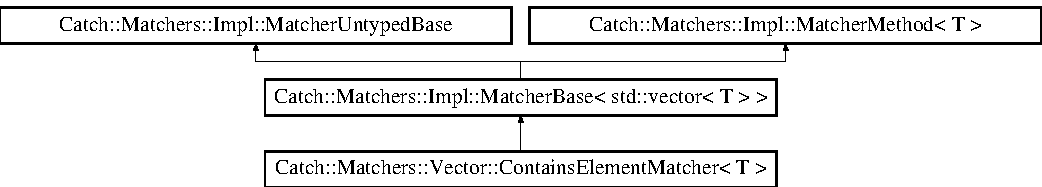
\includegraphics[height=2.514970cm]{struct_catch_1_1_matchers_1_1_vector_1_1_contains_element_matcher}
\end{center}
\end{figure}
\subsection*{Public Member Functions}
\begin{DoxyCompactItemize}
\item 
\mbox{\hyperlink{struct_catch_1_1_matchers_1_1_vector_1_1_contains_element_matcher_a6a05740b5d3f89fac8de84ac0cff7b93}{Contains\+Element\+Matcher}} (T const \&comparator)
\item 
bool \mbox{\hyperlink{struct_catch_1_1_matchers_1_1_vector_1_1_contains_element_matcher_a6a4be6e5642e267433d370649beb0fac}{match}} (std\+::vector$<$ T $>$ const \&v) const override
\item 
std\+::string \mbox{\hyperlink{struct_catch_1_1_matchers_1_1_vector_1_1_contains_element_matcher_aea3b674389a0afd82af6ba4b10f86ae6}{describe}} () const override
\end{DoxyCompactItemize}
\subsection*{Public Attributes}
\begin{DoxyCompactItemize}
\item 
T const  \& \mbox{\hyperlink{struct_catch_1_1_matchers_1_1_vector_1_1_contains_element_matcher_ab7eada6c4bbce1d21b44773262f9cb23}{m\+\_\+comparator}}
\end{DoxyCompactItemize}
\subsection*{Additional Inherited Members}


\subsection{Detailed Description}
\subsubsection*{template$<$typename T$>$\newline
struct Catch\+::\+Matchers\+::\+Vector\+::\+Contains\+Element\+Matcher$<$ T $>$}



Definition at line 2460 of file catch.\+hpp.



\subsection{Constructor \& Destructor Documentation}
\mbox{\Hypertarget{struct_catch_1_1_matchers_1_1_vector_1_1_contains_element_matcher_a6a05740b5d3f89fac8de84ac0cff7b93}\label{struct_catch_1_1_matchers_1_1_vector_1_1_contains_element_matcher_a6a05740b5d3f89fac8de84ac0cff7b93}} 
\index{Catch\+::\+Matchers\+::\+Vector\+::\+Contains\+Element\+Matcher@{Catch\+::\+Matchers\+::\+Vector\+::\+Contains\+Element\+Matcher}!Contains\+Element\+Matcher@{Contains\+Element\+Matcher}}
\index{Contains\+Element\+Matcher@{Contains\+Element\+Matcher}!Catch\+::\+Matchers\+::\+Vector\+::\+Contains\+Element\+Matcher@{Catch\+::\+Matchers\+::\+Vector\+::\+Contains\+Element\+Matcher}}
\subsubsection{\texorpdfstring{Contains\+Element\+Matcher()}{ContainsElementMatcher()}}
{\footnotesize\ttfamily template$<$typename T $>$ \\
\mbox{\hyperlink{struct_catch_1_1_matchers_1_1_vector_1_1_contains_element_matcher}{Catch\+::\+Matchers\+::\+Vector\+::\+Contains\+Element\+Matcher}}$<$ T $>$\+::\mbox{\hyperlink{struct_catch_1_1_matchers_1_1_vector_1_1_contains_element_matcher}{Contains\+Element\+Matcher}} (\begin{DoxyParamCaption}\item[{T const \&}]{comparator }\end{DoxyParamCaption})\hspace{0.3cm}{\ttfamily [inline]}}



Definition at line 2462 of file catch.\+hpp.



\subsection{Member Function Documentation}
\mbox{\Hypertarget{struct_catch_1_1_matchers_1_1_vector_1_1_contains_element_matcher_aea3b674389a0afd82af6ba4b10f86ae6}\label{struct_catch_1_1_matchers_1_1_vector_1_1_contains_element_matcher_aea3b674389a0afd82af6ba4b10f86ae6}} 
\index{Catch\+::\+Matchers\+::\+Vector\+::\+Contains\+Element\+Matcher@{Catch\+::\+Matchers\+::\+Vector\+::\+Contains\+Element\+Matcher}!describe@{describe}}
\index{describe@{describe}!Catch\+::\+Matchers\+::\+Vector\+::\+Contains\+Element\+Matcher@{Catch\+::\+Matchers\+::\+Vector\+::\+Contains\+Element\+Matcher}}
\subsubsection{\texorpdfstring{describe()}{describe()}}
{\footnotesize\ttfamily template$<$typename T $>$ \\
std\+::string \mbox{\hyperlink{struct_catch_1_1_matchers_1_1_vector_1_1_contains_element_matcher}{Catch\+::\+Matchers\+::\+Vector\+::\+Contains\+Element\+Matcher}}$<$ T $>$\+::describe (\begin{DoxyParamCaption}{ }\end{DoxyParamCaption}) const\hspace{0.3cm}{\ttfamily [inline]}, {\ttfamily [override]}, {\ttfamily [virtual]}}



Implements \mbox{\hyperlink{class_catch_1_1_matchers_1_1_impl_1_1_matcher_untyped_base_a91d3a907dbfcbb596077df24f6e11fe2}{Catch\+::\+Matchers\+::\+Impl\+::\+Matcher\+Untyped\+Base}}.



Definition at line 2473 of file catch.\+hpp.

\mbox{\Hypertarget{struct_catch_1_1_matchers_1_1_vector_1_1_contains_element_matcher_a6a4be6e5642e267433d370649beb0fac}\label{struct_catch_1_1_matchers_1_1_vector_1_1_contains_element_matcher_a6a4be6e5642e267433d370649beb0fac}} 
\index{Catch\+::\+Matchers\+::\+Vector\+::\+Contains\+Element\+Matcher@{Catch\+::\+Matchers\+::\+Vector\+::\+Contains\+Element\+Matcher}!match@{match}}
\index{match@{match}!Catch\+::\+Matchers\+::\+Vector\+::\+Contains\+Element\+Matcher@{Catch\+::\+Matchers\+::\+Vector\+::\+Contains\+Element\+Matcher}}
\subsubsection{\texorpdfstring{match()}{match()}}
{\footnotesize\ttfamily template$<$typename T $>$ \\
bool \mbox{\hyperlink{struct_catch_1_1_matchers_1_1_vector_1_1_contains_element_matcher}{Catch\+::\+Matchers\+::\+Vector\+::\+Contains\+Element\+Matcher}}$<$ T $>$\+::match (\begin{DoxyParamCaption}\item[{std\+::vector$<$ T $>$ const \&}]{v }\end{DoxyParamCaption}) const\hspace{0.3cm}{\ttfamily [inline]}, {\ttfamily [override]}}



Definition at line 2464 of file catch.\+hpp.



\subsection{Member Data Documentation}
\mbox{\Hypertarget{struct_catch_1_1_matchers_1_1_vector_1_1_contains_element_matcher_ab7eada6c4bbce1d21b44773262f9cb23}\label{struct_catch_1_1_matchers_1_1_vector_1_1_contains_element_matcher_ab7eada6c4bbce1d21b44773262f9cb23}} 
\index{Catch\+::\+Matchers\+::\+Vector\+::\+Contains\+Element\+Matcher@{Catch\+::\+Matchers\+::\+Vector\+::\+Contains\+Element\+Matcher}!m\+\_\+comparator@{m\+\_\+comparator}}
\index{m\+\_\+comparator@{m\+\_\+comparator}!Catch\+::\+Matchers\+::\+Vector\+::\+Contains\+Element\+Matcher@{Catch\+::\+Matchers\+::\+Vector\+::\+Contains\+Element\+Matcher}}
\subsubsection{\texorpdfstring{m\+\_\+comparator}{m\_comparator}}
{\footnotesize\ttfamily template$<$typename T $>$ \\
T const\& \mbox{\hyperlink{struct_catch_1_1_matchers_1_1_vector_1_1_contains_element_matcher}{Catch\+::\+Matchers\+::\+Vector\+::\+Contains\+Element\+Matcher}}$<$ T $>$\+::m\+\_\+comparator}



Definition at line 2477 of file catch.\+hpp.



The documentation for this struct was generated from the following file\+:\begin{DoxyCompactItemize}
\item 
D\+:/c++/block\+\_\+matrix-\/master/block\+\_\+matrix-\/master/test/\mbox{\hyperlink{catch_8hpp}{catch.\+hpp}}\end{DoxyCompactItemize}

\hypertarget{struct_catch_1_1_matchers_1_1_std_string_1_1_contains_matcher}{}\section{Catch\+:\+:Matchers\+:\+:Std\+String\+:\+:Contains\+Matcher Struct Reference}
\label{struct_catch_1_1_matchers_1_1_std_string_1_1_contains_matcher}\index{Catch\+::\+Matchers\+::\+Std\+String\+::\+Contains\+Matcher@{Catch\+::\+Matchers\+::\+Std\+String\+::\+Contains\+Matcher}}


{\ttfamily \#include $<$catch.\+hpp$>$}

Inheritance diagram for Catch\+:\+:Matchers\+:\+:Std\+String\+:\+:Contains\+Matcher\+:\begin{figure}[H]
\begin{center}
\leavevmode
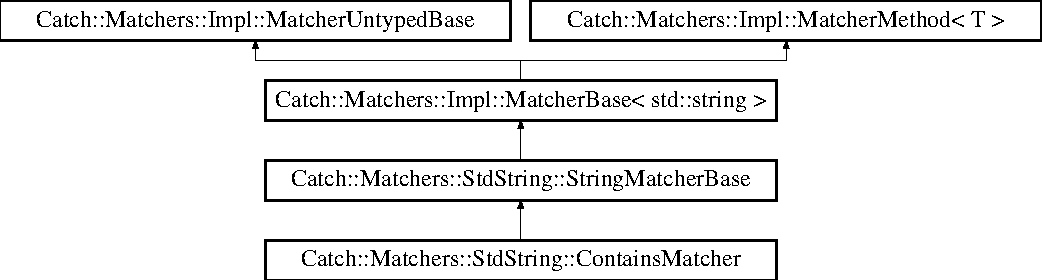
\includegraphics[height=3.758389cm]{struct_catch_1_1_matchers_1_1_std_string_1_1_contains_matcher}
\end{center}
\end{figure}
\subsection*{Public Member Functions}
\begin{DoxyCompactItemize}
\item 
\mbox{\hyperlink{struct_catch_1_1_matchers_1_1_std_string_1_1_contains_matcher_acc892883c8409e34b28c9b39d4ef1fe3}{Contains\+Matcher}} (\mbox{\hyperlink{struct_catch_1_1_matchers_1_1_std_string_1_1_cased_string}{Cased\+String}} const \&comparator)
\item 
bool \mbox{\hyperlink{struct_catch_1_1_matchers_1_1_std_string_1_1_contains_matcher_a630628b234b037be83fe587081a80b53}{match}} (std\+::string const \&source) const override
\end{DoxyCompactItemize}
\subsection*{Additional Inherited Members}


\subsection{Detailed Description}


Definition at line 2391 of file catch.\+hpp.



\subsection{Constructor \& Destructor Documentation}
\mbox{\Hypertarget{struct_catch_1_1_matchers_1_1_std_string_1_1_contains_matcher_acc892883c8409e34b28c9b39d4ef1fe3}\label{struct_catch_1_1_matchers_1_1_std_string_1_1_contains_matcher_acc892883c8409e34b28c9b39d4ef1fe3}} 
\index{Catch\+::\+Matchers\+::\+Std\+String\+::\+Contains\+Matcher@{Catch\+::\+Matchers\+::\+Std\+String\+::\+Contains\+Matcher}!Contains\+Matcher@{Contains\+Matcher}}
\index{Contains\+Matcher@{Contains\+Matcher}!Catch\+::\+Matchers\+::\+Std\+String\+::\+Contains\+Matcher@{Catch\+::\+Matchers\+::\+Std\+String\+::\+Contains\+Matcher}}
\subsubsection{\texorpdfstring{Contains\+Matcher()}{ContainsMatcher()}}
{\footnotesize\ttfamily Catch\+::\+Matchers\+::\+Std\+String\+::\+Contains\+Matcher\+::\+Contains\+Matcher (\begin{DoxyParamCaption}\item[{\mbox{\hyperlink{struct_catch_1_1_matchers_1_1_std_string_1_1_cased_string}{Cased\+String}} const \&}]{comparator }\end{DoxyParamCaption})}



\subsection{Member Function Documentation}
\mbox{\Hypertarget{struct_catch_1_1_matchers_1_1_std_string_1_1_contains_matcher_a630628b234b037be83fe587081a80b53}\label{struct_catch_1_1_matchers_1_1_std_string_1_1_contains_matcher_a630628b234b037be83fe587081a80b53}} 
\index{Catch\+::\+Matchers\+::\+Std\+String\+::\+Contains\+Matcher@{Catch\+::\+Matchers\+::\+Std\+String\+::\+Contains\+Matcher}!match@{match}}
\index{match@{match}!Catch\+::\+Matchers\+::\+Std\+String\+::\+Contains\+Matcher@{Catch\+::\+Matchers\+::\+Std\+String\+::\+Contains\+Matcher}}
\subsubsection{\texorpdfstring{match()}{match()}}
{\footnotesize\ttfamily bool Catch\+::\+Matchers\+::\+Std\+String\+::\+Contains\+Matcher\+::match (\begin{DoxyParamCaption}\item[{std\+::string const \&}]{source }\end{DoxyParamCaption}) const\hspace{0.3cm}{\ttfamily [override]}}



The documentation for this struct was generated from the following file\+:\begin{DoxyCompactItemize}
\item 
D\+:/c++/block\+\_\+matrix-\/master/block\+\_\+matrix-\/master/test/\mbox{\hyperlink{catch_8hpp}{catch.\+hpp}}\end{DoxyCompactItemize}

\hypertarget{struct_catch_1_1_matchers_1_1_vector_1_1_contains_matcher}{}\section{Catch\+:\+:Matchers\+:\+:Vector\+:\+:Contains\+Matcher$<$ T $>$ Struct Template Reference}
\label{struct_catch_1_1_matchers_1_1_vector_1_1_contains_matcher}\index{Catch\+::\+Matchers\+::\+Vector\+::\+Contains\+Matcher$<$ T $>$@{Catch\+::\+Matchers\+::\+Vector\+::\+Contains\+Matcher$<$ T $>$}}


{\ttfamily \#include $<$catch.\+hpp$>$}

Inheritance diagram for Catch\+:\+:Matchers\+:\+:Vector\+:\+:Contains\+Matcher$<$ T $>$\+:\begin{figure}[H]
\begin{center}
\leavevmode
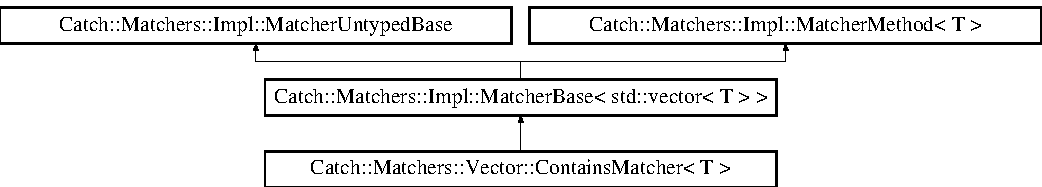
\includegraphics[height=2.514970cm]{struct_catch_1_1_matchers_1_1_vector_1_1_contains_matcher}
\end{center}
\end{figure}
\subsection*{Public Member Functions}
\begin{DoxyCompactItemize}
\item 
\mbox{\hyperlink{struct_catch_1_1_matchers_1_1_vector_1_1_contains_matcher_ad8e92c8399be6dce75bb5702cdfab700}{Contains\+Matcher}} (std\+::vector$<$ T $>$ const \&comparator)
\item 
bool \mbox{\hyperlink{struct_catch_1_1_matchers_1_1_vector_1_1_contains_matcher_afd33467ae48a41a634572b41b053f67f}{match}} (std\+::vector$<$ T $>$ const \&v) const override
\item 
std\+::string \mbox{\hyperlink{struct_catch_1_1_matchers_1_1_vector_1_1_contains_matcher_abe6a9ea3d6506c9a1f75ff524f35832e}{describe}} () const override
\end{DoxyCompactItemize}
\subsection*{Public Attributes}
\begin{DoxyCompactItemize}
\item 
std\+::vector$<$ T $>$ const  \& \mbox{\hyperlink{struct_catch_1_1_matchers_1_1_vector_1_1_contains_matcher_a83d051166e4ed0d535219ad6ee99abb2}{m\+\_\+comparator}}
\end{DoxyCompactItemize}
\subsection*{Additional Inherited Members}


\subsection{Detailed Description}
\subsubsection*{template$<$typename T$>$\newline
struct Catch\+::\+Matchers\+::\+Vector\+::\+Contains\+Matcher$<$ T $>$}



Definition at line 2481 of file catch.\+hpp.



\subsection{Constructor \& Destructor Documentation}
\mbox{\Hypertarget{struct_catch_1_1_matchers_1_1_vector_1_1_contains_matcher_ad8e92c8399be6dce75bb5702cdfab700}\label{struct_catch_1_1_matchers_1_1_vector_1_1_contains_matcher_ad8e92c8399be6dce75bb5702cdfab700}} 
\index{Catch\+::\+Matchers\+::\+Vector\+::\+Contains\+Matcher@{Catch\+::\+Matchers\+::\+Vector\+::\+Contains\+Matcher}!Contains\+Matcher@{Contains\+Matcher}}
\index{Contains\+Matcher@{Contains\+Matcher}!Catch\+::\+Matchers\+::\+Vector\+::\+Contains\+Matcher@{Catch\+::\+Matchers\+::\+Vector\+::\+Contains\+Matcher}}
\subsubsection{\texorpdfstring{Contains\+Matcher()}{ContainsMatcher()}}
{\footnotesize\ttfamily template$<$typename T $>$ \\
\mbox{\hyperlink{struct_catch_1_1_matchers_1_1_vector_1_1_contains_matcher}{Catch\+::\+Matchers\+::\+Vector\+::\+Contains\+Matcher}}$<$ T $>$\+::\mbox{\hyperlink{struct_catch_1_1_matchers_1_1_vector_1_1_contains_matcher}{Contains\+Matcher}} (\begin{DoxyParamCaption}\item[{std\+::vector$<$ T $>$ const \&}]{comparator }\end{DoxyParamCaption})\hspace{0.3cm}{\ttfamily [inline]}}



Definition at line 2483 of file catch.\+hpp.



\subsection{Member Function Documentation}
\mbox{\Hypertarget{struct_catch_1_1_matchers_1_1_vector_1_1_contains_matcher_abe6a9ea3d6506c9a1f75ff524f35832e}\label{struct_catch_1_1_matchers_1_1_vector_1_1_contains_matcher_abe6a9ea3d6506c9a1f75ff524f35832e}} 
\index{Catch\+::\+Matchers\+::\+Vector\+::\+Contains\+Matcher@{Catch\+::\+Matchers\+::\+Vector\+::\+Contains\+Matcher}!describe@{describe}}
\index{describe@{describe}!Catch\+::\+Matchers\+::\+Vector\+::\+Contains\+Matcher@{Catch\+::\+Matchers\+::\+Vector\+::\+Contains\+Matcher}}
\subsubsection{\texorpdfstring{describe()}{describe()}}
{\footnotesize\ttfamily template$<$typename T $>$ \\
std\+::string \mbox{\hyperlink{struct_catch_1_1_matchers_1_1_vector_1_1_contains_matcher}{Catch\+::\+Matchers\+::\+Vector\+::\+Contains\+Matcher}}$<$ T $>$\+::describe (\begin{DoxyParamCaption}{ }\end{DoxyParamCaption}) const\hspace{0.3cm}{\ttfamily [inline]}, {\ttfamily [override]}, {\ttfamily [virtual]}}



Implements \mbox{\hyperlink{class_catch_1_1_matchers_1_1_impl_1_1_matcher_untyped_base_a91d3a907dbfcbb596077df24f6e11fe2}{Catch\+::\+Matchers\+::\+Impl\+::\+Matcher\+Untyped\+Base}}.



Definition at line 2503 of file catch.\+hpp.

\mbox{\Hypertarget{struct_catch_1_1_matchers_1_1_vector_1_1_contains_matcher_afd33467ae48a41a634572b41b053f67f}\label{struct_catch_1_1_matchers_1_1_vector_1_1_contains_matcher_afd33467ae48a41a634572b41b053f67f}} 
\index{Catch\+::\+Matchers\+::\+Vector\+::\+Contains\+Matcher@{Catch\+::\+Matchers\+::\+Vector\+::\+Contains\+Matcher}!match@{match}}
\index{match@{match}!Catch\+::\+Matchers\+::\+Vector\+::\+Contains\+Matcher@{Catch\+::\+Matchers\+::\+Vector\+::\+Contains\+Matcher}}
\subsubsection{\texorpdfstring{match()}{match()}}
{\footnotesize\ttfamily template$<$typename T $>$ \\
bool \mbox{\hyperlink{struct_catch_1_1_matchers_1_1_vector_1_1_contains_matcher}{Catch\+::\+Matchers\+::\+Vector\+::\+Contains\+Matcher}}$<$ T $>$\+::match (\begin{DoxyParamCaption}\item[{std\+::vector$<$ T $>$ const \&}]{v }\end{DoxyParamCaption}) const\hspace{0.3cm}{\ttfamily [inline]}, {\ttfamily [override]}}



Definition at line 2485 of file catch.\+hpp.



\subsection{Member Data Documentation}
\mbox{\Hypertarget{struct_catch_1_1_matchers_1_1_vector_1_1_contains_matcher_a83d051166e4ed0d535219ad6ee99abb2}\label{struct_catch_1_1_matchers_1_1_vector_1_1_contains_matcher_a83d051166e4ed0d535219ad6ee99abb2}} 
\index{Catch\+::\+Matchers\+::\+Vector\+::\+Contains\+Matcher@{Catch\+::\+Matchers\+::\+Vector\+::\+Contains\+Matcher}!m\+\_\+comparator@{m\+\_\+comparator}}
\index{m\+\_\+comparator@{m\+\_\+comparator}!Catch\+::\+Matchers\+::\+Vector\+::\+Contains\+Matcher@{Catch\+::\+Matchers\+::\+Vector\+::\+Contains\+Matcher}}
\subsubsection{\texorpdfstring{m\+\_\+comparator}{m\_comparator}}
{\footnotesize\ttfamily template$<$typename T $>$ \\
std\+::vector$<$T$>$ const\& \mbox{\hyperlink{struct_catch_1_1_matchers_1_1_vector_1_1_contains_matcher}{Catch\+::\+Matchers\+::\+Vector\+::\+Contains\+Matcher}}$<$ T $>$\+::m\+\_\+comparator}



Definition at line 2507 of file catch.\+hpp.



The documentation for this struct was generated from the following file\+:\begin{DoxyCompactItemize}
\item 
D\+:/c++/block\+\_\+matrix-\/master/block\+\_\+matrix-\/master/test/\mbox{\hyperlink{catch_8hpp}{catch.\+hpp}}\end{DoxyCompactItemize}

\hypertarget{struct_catch_1_1_counts}{}\section{Catch\+:\+:Counts Struct Reference}
\label{struct_catch_1_1_counts}\index{Catch\+::\+Counts@{Catch\+::\+Counts}}


{\ttfamily \#include $<$catch.\+hpp$>$}

\subsection*{Public Member Functions}
\begin{DoxyCompactItemize}
\item 
\mbox{\hyperlink{struct_catch_1_1_counts}{Counts}} \mbox{\hyperlink{struct_catch_1_1_counts_aaa10666f559057e3e860d2a5a6fae4c4}{operator-\/}} (\mbox{\hyperlink{struct_catch_1_1_counts}{Counts}} const \&other) const
\item 
\mbox{\hyperlink{struct_catch_1_1_counts}{Counts}} \& \mbox{\hyperlink{struct_catch_1_1_counts_a322a89475cd2cc039140ef371e973677}{operator+=}} (\mbox{\hyperlink{struct_catch_1_1_counts}{Counts}} const \&other)
\item 
std\+::size\+\_\+t \mbox{\hyperlink{struct_catch_1_1_counts_a94f969c09cf52d1339c085c9603cd1d3}{total}} () const
\item 
bool \mbox{\hyperlink{struct_catch_1_1_counts_a84999490e0ecaa3de5e121bf48eda1b3}{all\+Passed}} () const
\item 
bool \mbox{\hyperlink{struct_catch_1_1_counts_a33bd996e016030155b99fe1c51c08991}{all\+Ok}} () const
\end{DoxyCompactItemize}
\subsection*{Public Attributes}
\begin{DoxyCompactItemize}
\item 
std\+::size\+\_\+t \mbox{\hyperlink{struct_catch_1_1_counts_ad28daaf3de28006400208b6dd0c631e6}{passed}} = 0
\item 
std\+::size\+\_\+t \mbox{\hyperlink{struct_catch_1_1_counts_a19982a3817a3bc2c07f0290e71f497a3}{failed}} = 0
\item 
std\+::size\+\_\+t \mbox{\hyperlink{struct_catch_1_1_counts_ac090973a2ff51394cd452718e75c073e}{failed\+But\+Ok}} = 0
\end{DoxyCompactItemize}


\subsection{Detailed Description}


Definition at line 1748 of file catch.\+hpp.



\subsection{Member Function Documentation}
\mbox{\Hypertarget{struct_catch_1_1_counts_a33bd996e016030155b99fe1c51c08991}\label{struct_catch_1_1_counts_a33bd996e016030155b99fe1c51c08991}} 
\index{Catch\+::\+Counts@{Catch\+::\+Counts}!all\+Ok@{all\+Ok}}
\index{all\+Ok@{all\+Ok}!Catch\+::\+Counts@{Catch\+::\+Counts}}
\subsubsection{\texorpdfstring{all\+Ok()}{allOk()}}
{\footnotesize\ttfamily bool Catch\+::\+Counts\+::all\+Ok (\begin{DoxyParamCaption}{ }\end{DoxyParamCaption}) const}

\mbox{\Hypertarget{struct_catch_1_1_counts_a84999490e0ecaa3de5e121bf48eda1b3}\label{struct_catch_1_1_counts_a84999490e0ecaa3de5e121bf48eda1b3}} 
\index{Catch\+::\+Counts@{Catch\+::\+Counts}!all\+Passed@{all\+Passed}}
\index{all\+Passed@{all\+Passed}!Catch\+::\+Counts@{Catch\+::\+Counts}}
\subsubsection{\texorpdfstring{all\+Passed()}{allPassed()}}
{\footnotesize\ttfamily bool Catch\+::\+Counts\+::all\+Passed (\begin{DoxyParamCaption}{ }\end{DoxyParamCaption}) const}

\mbox{\Hypertarget{struct_catch_1_1_counts_a322a89475cd2cc039140ef371e973677}\label{struct_catch_1_1_counts_a322a89475cd2cc039140ef371e973677}} 
\index{Catch\+::\+Counts@{Catch\+::\+Counts}!operator+=@{operator+=}}
\index{operator+=@{operator+=}!Catch\+::\+Counts@{Catch\+::\+Counts}}
\subsubsection{\texorpdfstring{operator+=()}{operator+=()}}
{\footnotesize\ttfamily \mbox{\hyperlink{struct_catch_1_1_counts}{Counts}}\& Catch\+::\+Counts\+::operator+= (\begin{DoxyParamCaption}\item[{\mbox{\hyperlink{struct_catch_1_1_counts}{Counts}} const \&}]{other }\end{DoxyParamCaption})}

\mbox{\Hypertarget{struct_catch_1_1_counts_aaa10666f559057e3e860d2a5a6fae4c4}\label{struct_catch_1_1_counts_aaa10666f559057e3e860d2a5a6fae4c4}} 
\index{Catch\+::\+Counts@{Catch\+::\+Counts}!operator-\/@{operator-\/}}
\index{operator-\/@{operator-\/}!Catch\+::\+Counts@{Catch\+::\+Counts}}
\subsubsection{\texorpdfstring{operator-\/()}{operator-()}}
{\footnotesize\ttfamily \mbox{\hyperlink{struct_catch_1_1_counts}{Counts}} Catch\+::\+Counts\+::operator-\/ (\begin{DoxyParamCaption}\item[{\mbox{\hyperlink{struct_catch_1_1_counts}{Counts}} const \&}]{other }\end{DoxyParamCaption}) const}

\mbox{\Hypertarget{struct_catch_1_1_counts_a94f969c09cf52d1339c085c9603cd1d3}\label{struct_catch_1_1_counts_a94f969c09cf52d1339c085c9603cd1d3}} 
\index{Catch\+::\+Counts@{Catch\+::\+Counts}!total@{total}}
\index{total@{total}!Catch\+::\+Counts@{Catch\+::\+Counts}}
\subsubsection{\texorpdfstring{total()}{total()}}
{\footnotesize\ttfamily std\+::size\+\_\+t Catch\+::\+Counts\+::total (\begin{DoxyParamCaption}{ }\end{DoxyParamCaption}) const}



\subsection{Member Data Documentation}
\mbox{\Hypertarget{struct_catch_1_1_counts_a19982a3817a3bc2c07f0290e71f497a3}\label{struct_catch_1_1_counts_a19982a3817a3bc2c07f0290e71f497a3}} 
\index{Catch\+::\+Counts@{Catch\+::\+Counts}!failed@{failed}}
\index{failed@{failed}!Catch\+::\+Counts@{Catch\+::\+Counts}}
\subsubsection{\texorpdfstring{failed}{failed}}
{\footnotesize\ttfamily std\+::size\+\_\+t Catch\+::\+Counts\+::failed = 0}



Definition at line 1757 of file catch.\+hpp.

\mbox{\Hypertarget{struct_catch_1_1_counts_ac090973a2ff51394cd452718e75c073e}\label{struct_catch_1_1_counts_ac090973a2ff51394cd452718e75c073e}} 
\index{Catch\+::\+Counts@{Catch\+::\+Counts}!failed\+But\+Ok@{failed\+But\+Ok}}
\index{failed\+But\+Ok@{failed\+But\+Ok}!Catch\+::\+Counts@{Catch\+::\+Counts}}
\subsubsection{\texorpdfstring{failed\+But\+Ok}{failedButOk}}
{\footnotesize\ttfamily std\+::size\+\_\+t Catch\+::\+Counts\+::failed\+But\+Ok = 0}



Definition at line 1758 of file catch.\+hpp.

\mbox{\Hypertarget{struct_catch_1_1_counts_ad28daaf3de28006400208b6dd0c631e6}\label{struct_catch_1_1_counts_ad28daaf3de28006400208b6dd0c631e6}} 
\index{Catch\+::\+Counts@{Catch\+::\+Counts}!passed@{passed}}
\index{passed@{passed}!Catch\+::\+Counts@{Catch\+::\+Counts}}
\subsubsection{\texorpdfstring{passed}{passed}}
{\footnotesize\ttfamily std\+::size\+\_\+t Catch\+::\+Counts\+::passed = 0}



Definition at line 1756 of file catch.\+hpp.



The documentation for this struct was generated from the following file\+:\begin{DoxyCompactItemize}
\item 
D\+:/c++/block\+\_\+matrix-\/master/block\+\_\+matrix-\/master/test/\mbox{\hyperlink{catch_8hpp}{catch.\+hpp}}\end{DoxyCompactItemize}

\hypertarget{struct_catch_1_1_decomposer}{}\section{Catch\+:\+:Decomposer Struct Reference}
\label{struct_catch_1_1_decomposer}\index{Catch\+::\+Decomposer@{Catch\+::\+Decomposer}}


{\ttfamily \#include $<$catch.\+hpp$>$}

\subsection*{Public Member Functions}
\begin{DoxyCompactItemize}
\item 
{\footnotesize template$<$typename T $>$ }\\auto \mbox{\hyperlink{struct_catch_1_1_decomposer_a20b5b8c0e2ff0328a019ae1a8deca03a}{operator$<$=}} (T const \&lhs) -\/$>$ \mbox{\hyperlink{class_catch_1_1_expr_lhs}{Expr\+Lhs}}$<$ T const \&$>$
\item 
auto \mbox{\hyperlink{struct_catch_1_1_decomposer_aac129b94903ae1339d5709049d83613b}{operator$<$=}} (bool value) -\/$>$ \mbox{\hyperlink{class_catch_1_1_expr_lhs}{Expr\+Lhs}}$<$ bool $>$
\end{DoxyCompactItemize}


\subsection{Detailed Description}


Definition at line 1385 of file catch.\+hpp.



\subsection{Member Function Documentation}
\mbox{\Hypertarget{struct_catch_1_1_decomposer_a20b5b8c0e2ff0328a019ae1a8deca03a}\label{struct_catch_1_1_decomposer_a20b5b8c0e2ff0328a019ae1a8deca03a}} 
\index{Catch\+::\+Decomposer@{Catch\+::\+Decomposer}!operator$<$=@{operator$<$=}}
\index{operator$<$=@{operator$<$=}!Catch\+::\+Decomposer@{Catch\+::\+Decomposer}}
\subsubsection{\texorpdfstring{operator$<$=()}{operator<=()}\hspace{0.1cm}{\footnotesize\ttfamily [1/2]}}
{\footnotesize\ttfamily template$<$typename T $>$ \\
auto Catch\+::\+Decomposer\+::operator$<$= (\begin{DoxyParamCaption}\item[{T const \&}]{lhs }\end{DoxyParamCaption}) -\/$>$ \mbox{\hyperlink{class_catch_1_1_expr_lhs}{Expr\+Lhs}}$<$T const\&$>$ \hspace{0.3cm}{\ttfamily [inline]}}



Definition at line 1387 of file catch.\+hpp.

\mbox{\Hypertarget{struct_catch_1_1_decomposer_aac129b94903ae1339d5709049d83613b}\label{struct_catch_1_1_decomposer_aac129b94903ae1339d5709049d83613b}} 
\index{Catch\+::\+Decomposer@{Catch\+::\+Decomposer}!operator$<$=@{operator$<$=}}
\index{operator$<$=@{operator$<$=}!Catch\+::\+Decomposer@{Catch\+::\+Decomposer}}
\subsubsection{\texorpdfstring{operator$<$=()}{operator<=()}\hspace{0.1cm}{\footnotesize\ttfamily [2/2]}}
{\footnotesize\ttfamily auto Catch\+::\+Decomposer\+::operator$<$= (\begin{DoxyParamCaption}\item[{bool}]{value }\end{DoxyParamCaption}) -\/$>$ \mbox{\hyperlink{class_catch_1_1_expr_lhs}{Expr\+Lhs}}$<$bool$>$ \hspace{0.3cm}{\ttfamily [inline]}}



Definition at line 1391 of file catch.\+hpp.



The documentation for this struct was generated from the following file\+:\begin{DoxyCompactItemize}
\item 
D\+:/c++/block\+\_\+matrix-\/master/block\+\_\+matrix-\/master/test/\mbox{\hyperlink{catch_8hpp}{catch.\+hpp}}\end{DoxyCompactItemize}

\hypertarget{struct_catch_1_1_matchers_1_1_std_string_1_1_ends_with_matcher}{}\section{Catch\+:\+:Matchers\+:\+:Std\+String\+:\+:Ends\+With\+Matcher Struct Reference}
\label{struct_catch_1_1_matchers_1_1_std_string_1_1_ends_with_matcher}\index{Catch\+::\+Matchers\+::\+Std\+String\+::\+Ends\+With\+Matcher@{Catch\+::\+Matchers\+::\+Std\+String\+::\+Ends\+With\+Matcher}}


{\ttfamily \#include $<$catch.\+hpp$>$}

Inheritance diagram for Catch\+:\+:Matchers\+:\+:Std\+String\+:\+:Ends\+With\+Matcher\+:\begin{figure}[H]
\begin{center}
\leavevmode
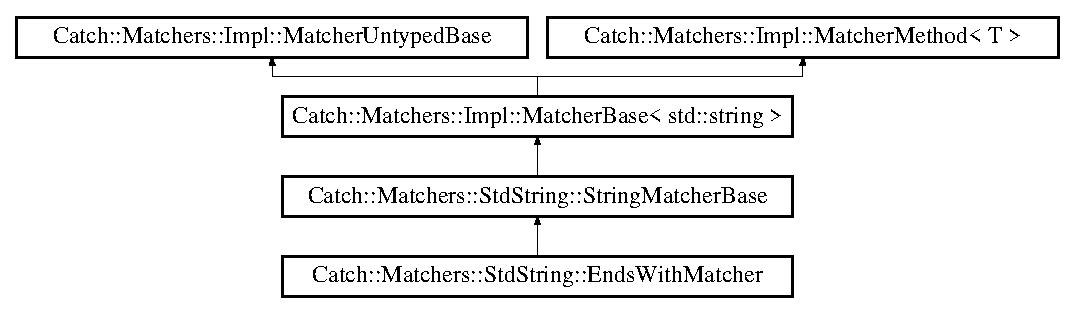
\includegraphics[height=3.758389cm]{struct_catch_1_1_matchers_1_1_std_string_1_1_ends_with_matcher}
\end{center}
\end{figure}
\subsection*{Public Member Functions}
\begin{DoxyCompactItemize}
\item 
\mbox{\hyperlink{struct_catch_1_1_matchers_1_1_std_string_1_1_ends_with_matcher_aa5ec700b4629562f74f362080accfd7b}{Ends\+With\+Matcher}} (\mbox{\hyperlink{struct_catch_1_1_matchers_1_1_std_string_1_1_cased_string}{Cased\+String}} const \&comparator)
\item 
bool \mbox{\hyperlink{struct_catch_1_1_matchers_1_1_std_string_1_1_ends_with_matcher_aca2741fa57374a2a98d2a84ac3e13a6d}{match}} (std\+::string const \&source) const override
\end{DoxyCompactItemize}
\subsection*{Additional Inherited Members}


\subsection{Detailed Description}


Definition at line 2399 of file catch.\+hpp.



\subsection{Constructor \& Destructor Documentation}
\mbox{\Hypertarget{struct_catch_1_1_matchers_1_1_std_string_1_1_ends_with_matcher_aa5ec700b4629562f74f362080accfd7b}\label{struct_catch_1_1_matchers_1_1_std_string_1_1_ends_with_matcher_aa5ec700b4629562f74f362080accfd7b}} 
\index{Catch\+::\+Matchers\+::\+Std\+String\+::\+Ends\+With\+Matcher@{Catch\+::\+Matchers\+::\+Std\+String\+::\+Ends\+With\+Matcher}!Ends\+With\+Matcher@{Ends\+With\+Matcher}}
\index{Ends\+With\+Matcher@{Ends\+With\+Matcher}!Catch\+::\+Matchers\+::\+Std\+String\+::\+Ends\+With\+Matcher@{Catch\+::\+Matchers\+::\+Std\+String\+::\+Ends\+With\+Matcher}}
\subsubsection{\texorpdfstring{Ends\+With\+Matcher()}{EndsWithMatcher()}}
{\footnotesize\ttfamily Catch\+::\+Matchers\+::\+Std\+String\+::\+Ends\+With\+Matcher\+::\+Ends\+With\+Matcher (\begin{DoxyParamCaption}\item[{\mbox{\hyperlink{struct_catch_1_1_matchers_1_1_std_string_1_1_cased_string}{Cased\+String}} const \&}]{comparator }\end{DoxyParamCaption})}



\subsection{Member Function Documentation}
\mbox{\Hypertarget{struct_catch_1_1_matchers_1_1_std_string_1_1_ends_with_matcher_aca2741fa57374a2a98d2a84ac3e13a6d}\label{struct_catch_1_1_matchers_1_1_std_string_1_1_ends_with_matcher_aca2741fa57374a2a98d2a84ac3e13a6d}} 
\index{Catch\+::\+Matchers\+::\+Std\+String\+::\+Ends\+With\+Matcher@{Catch\+::\+Matchers\+::\+Std\+String\+::\+Ends\+With\+Matcher}!match@{match}}
\index{match@{match}!Catch\+::\+Matchers\+::\+Std\+String\+::\+Ends\+With\+Matcher@{Catch\+::\+Matchers\+::\+Std\+String\+::\+Ends\+With\+Matcher}}
\subsubsection{\texorpdfstring{match()}{match()}}
{\footnotesize\ttfamily bool Catch\+::\+Matchers\+::\+Std\+String\+::\+Ends\+With\+Matcher\+::match (\begin{DoxyParamCaption}\item[{std\+::string const \&}]{source }\end{DoxyParamCaption}) const\hspace{0.3cm}{\ttfamily [override]}}



The documentation for this struct was generated from the following file\+:\begin{DoxyCompactItemize}
\item 
D\+:/c++/block\+\_\+matrix-\/master/block\+\_\+matrix-\/master/test/\mbox{\hyperlink{catch_8hpp}{catch.\+hpp}}\end{DoxyCompactItemize}

\hypertarget{struct_catch_1_1_matchers_1_1_std_string_1_1_equals_matcher}{}\section{Catch\+:\+:Matchers\+:\+:Std\+String\+:\+:Equals\+Matcher Struct Reference}
\label{struct_catch_1_1_matchers_1_1_std_string_1_1_equals_matcher}\index{Catch\+::\+Matchers\+::\+Std\+String\+::\+Equals\+Matcher@{Catch\+::\+Matchers\+::\+Std\+String\+::\+Equals\+Matcher}}


{\ttfamily \#include $<$catch.\+hpp$>$}

Inheritance diagram for Catch\+:\+:Matchers\+:\+:Std\+String\+:\+:Equals\+Matcher\+:\begin{figure}[H]
\begin{center}
\leavevmode
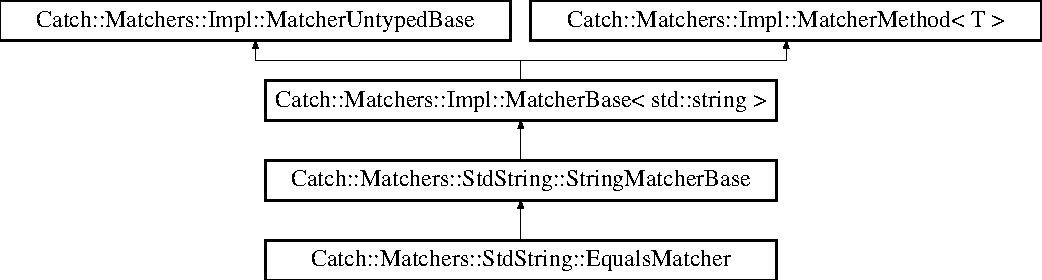
\includegraphics[height=3.758389cm]{struct_catch_1_1_matchers_1_1_std_string_1_1_equals_matcher}
\end{center}
\end{figure}
\subsection*{Public Member Functions}
\begin{DoxyCompactItemize}
\item 
\mbox{\hyperlink{struct_catch_1_1_matchers_1_1_std_string_1_1_equals_matcher_ab740f1fb2310e9fe3fed5134d4c7e4c8}{Equals\+Matcher}} (\mbox{\hyperlink{struct_catch_1_1_matchers_1_1_std_string_1_1_cased_string}{Cased\+String}} const \&comparator)
\item 
bool \mbox{\hyperlink{struct_catch_1_1_matchers_1_1_std_string_1_1_equals_matcher_a0bb9d64693f7bb1ef7441062d219f21a}{match}} (std\+::string const \&source) const override
\end{DoxyCompactItemize}
\subsection*{Additional Inherited Members}


\subsection{Detailed Description}


Definition at line 2387 of file catch.\+hpp.



\subsection{Constructor \& Destructor Documentation}
\mbox{\Hypertarget{struct_catch_1_1_matchers_1_1_std_string_1_1_equals_matcher_ab740f1fb2310e9fe3fed5134d4c7e4c8}\label{struct_catch_1_1_matchers_1_1_std_string_1_1_equals_matcher_ab740f1fb2310e9fe3fed5134d4c7e4c8}} 
\index{Catch\+::\+Matchers\+::\+Std\+String\+::\+Equals\+Matcher@{Catch\+::\+Matchers\+::\+Std\+String\+::\+Equals\+Matcher}!Equals\+Matcher@{Equals\+Matcher}}
\index{Equals\+Matcher@{Equals\+Matcher}!Catch\+::\+Matchers\+::\+Std\+String\+::\+Equals\+Matcher@{Catch\+::\+Matchers\+::\+Std\+String\+::\+Equals\+Matcher}}
\subsubsection{\texorpdfstring{Equals\+Matcher()}{EqualsMatcher()}}
{\footnotesize\ttfamily Catch\+::\+Matchers\+::\+Std\+String\+::\+Equals\+Matcher\+::\+Equals\+Matcher (\begin{DoxyParamCaption}\item[{\mbox{\hyperlink{struct_catch_1_1_matchers_1_1_std_string_1_1_cased_string}{Cased\+String}} const \&}]{comparator }\end{DoxyParamCaption})}



\subsection{Member Function Documentation}
\mbox{\Hypertarget{struct_catch_1_1_matchers_1_1_std_string_1_1_equals_matcher_a0bb9d64693f7bb1ef7441062d219f21a}\label{struct_catch_1_1_matchers_1_1_std_string_1_1_equals_matcher_a0bb9d64693f7bb1ef7441062d219f21a}} 
\index{Catch\+::\+Matchers\+::\+Std\+String\+::\+Equals\+Matcher@{Catch\+::\+Matchers\+::\+Std\+String\+::\+Equals\+Matcher}!match@{match}}
\index{match@{match}!Catch\+::\+Matchers\+::\+Std\+String\+::\+Equals\+Matcher@{Catch\+::\+Matchers\+::\+Std\+String\+::\+Equals\+Matcher}}
\subsubsection{\texorpdfstring{match()}{match()}}
{\footnotesize\ttfamily bool Catch\+::\+Matchers\+::\+Std\+String\+::\+Equals\+Matcher\+::match (\begin{DoxyParamCaption}\item[{std\+::string const \&}]{source }\end{DoxyParamCaption}) const\hspace{0.3cm}{\ttfamily [override]}}



The documentation for this struct was generated from the following file\+:\begin{DoxyCompactItemize}
\item 
D\+:/c++/block\+\_\+matrix-\/master/block\+\_\+matrix-\/master/test/\mbox{\hyperlink{catch_8hpp}{catch.\+hpp}}\end{DoxyCompactItemize}

\hypertarget{struct_catch_1_1_matchers_1_1_vector_1_1_equals_matcher}{}\section{Catch\+:\+:Matchers\+:\+:Vector\+:\+:Equals\+Matcher$<$ T $>$ Struct Template Reference}
\label{struct_catch_1_1_matchers_1_1_vector_1_1_equals_matcher}\index{Catch\+::\+Matchers\+::\+Vector\+::\+Equals\+Matcher$<$ T $>$@{Catch\+::\+Matchers\+::\+Vector\+::\+Equals\+Matcher$<$ T $>$}}


{\ttfamily \#include $<$catch.\+hpp$>$}

Inheritance diagram for Catch\+:\+:Matchers\+:\+:Vector\+:\+:Equals\+Matcher$<$ T $>$\+:\begin{figure}[H]
\begin{center}
\leavevmode
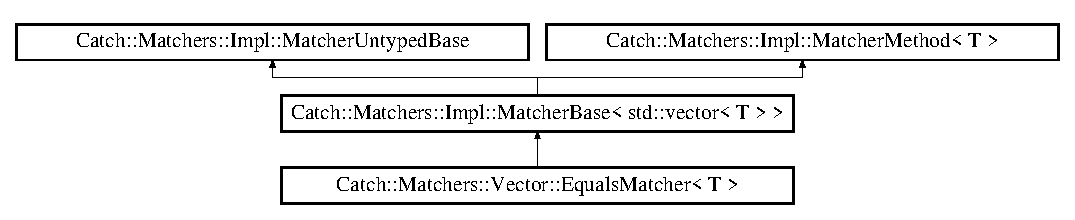
\includegraphics[height=2.514970cm]{struct_catch_1_1_matchers_1_1_vector_1_1_equals_matcher}
\end{center}
\end{figure}
\subsection*{Public Member Functions}
\begin{DoxyCompactItemize}
\item 
\mbox{\hyperlink{struct_catch_1_1_matchers_1_1_vector_1_1_equals_matcher_a3846c47780d1991dcfe87aefded98008}{Equals\+Matcher}} (std\+::vector$<$ T $>$ const \&comparator)
\item 
bool \mbox{\hyperlink{struct_catch_1_1_matchers_1_1_vector_1_1_equals_matcher_a2d96cca58a44151fddc5257eda3305da}{match}} (std\+::vector$<$ T $>$ const \&v) const override
\item 
std\+::string \mbox{\hyperlink{struct_catch_1_1_matchers_1_1_vector_1_1_equals_matcher_a36b5f7ecada4081d6c65bebe8ddea6f4}{describe}} () const override
\end{DoxyCompactItemize}
\subsection*{Public Attributes}
\begin{DoxyCompactItemize}
\item 
std\+::vector$<$ T $>$ const  \& \mbox{\hyperlink{struct_catch_1_1_matchers_1_1_vector_1_1_equals_matcher_a56f7aa6f110a12b1b9aeb0cabbc9d755}{m\+\_\+comparator}}
\end{DoxyCompactItemize}
\subsection*{Additional Inherited Members}


\subsection{Detailed Description}
\subsubsection*{template$<$typename T$>$\newline
struct Catch\+::\+Matchers\+::\+Vector\+::\+Equals\+Matcher$<$ T $>$}



Definition at line 2511 of file catch.\+hpp.



\subsection{Constructor \& Destructor Documentation}
\mbox{\Hypertarget{struct_catch_1_1_matchers_1_1_vector_1_1_equals_matcher_a3846c47780d1991dcfe87aefded98008}\label{struct_catch_1_1_matchers_1_1_vector_1_1_equals_matcher_a3846c47780d1991dcfe87aefded98008}} 
\index{Catch\+::\+Matchers\+::\+Vector\+::\+Equals\+Matcher@{Catch\+::\+Matchers\+::\+Vector\+::\+Equals\+Matcher}!Equals\+Matcher@{Equals\+Matcher}}
\index{Equals\+Matcher@{Equals\+Matcher}!Catch\+::\+Matchers\+::\+Vector\+::\+Equals\+Matcher@{Catch\+::\+Matchers\+::\+Vector\+::\+Equals\+Matcher}}
\subsubsection{\texorpdfstring{Equals\+Matcher()}{EqualsMatcher()}}
{\footnotesize\ttfamily template$<$typename T $>$ \\
\mbox{\hyperlink{struct_catch_1_1_matchers_1_1_vector_1_1_equals_matcher}{Catch\+::\+Matchers\+::\+Vector\+::\+Equals\+Matcher}}$<$ T $>$\+::\mbox{\hyperlink{struct_catch_1_1_matchers_1_1_vector_1_1_equals_matcher}{Equals\+Matcher}} (\begin{DoxyParamCaption}\item[{std\+::vector$<$ T $>$ const \&}]{comparator }\end{DoxyParamCaption})\hspace{0.3cm}{\ttfamily [inline]}}



Definition at line 2513 of file catch.\+hpp.



\subsection{Member Function Documentation}
\mbox{\Hypertarget{struct_catch_1_1_matchers_1_1_vector_1_1_equals_matcher_a36b5f7ecada4081d6c65bebe8ddea6f4}\label{struct_catch_1_1_matchers_1_1_vector_1_1_equals_matcher_a36b5f7ecada4081d6c65bebe8ddea6f4}} 
\index{Catch\+::\+Matchers\+::\+Vector\+::\+Equals\+Matcher@{Catch\+::\+Matchers\+::\+Vector\+::\+Equals\+Matcher}!describe@{describe}}
\index{describe@{describe}!Catch\+::\+Matchers\+::\+Vector\+::\+Equals\+Matcher@{Catch\+::\+Matchers\+::\+Vector\+::\+Equals\+Matcher}}
\subsubsection{\texorpdfstring{describe()}{describe()}}
{\footnotesize\ttfamily template$<$typename T $>$ \\
std\+::string \mbox{\hyperlink{struct_catch_1_1_matchers_1_1_vector_1_1_equals_matcher}{Catch\+::\+Matchers\+::\+Vector\+::\+Equals\+Matcher}}$<$ T $>$\+::describe (\begin{DoxyParamCaption}{ }\end{DoxyParamCaption}) const\hspace{0.3cm}{\ttfamily [inline]}, {\ttfamily [override]}, {\ttfamily [virtual]}}



Implements \mbox{\hyperlink{class_catch_1_1_matchers_1_1_impl_1_1_matcher_untyped_base_a91d3a907dbfcbb596077df24f6e11fe2}{Catch\+::\+Matchers\+::\+Impl\+::\+Matcher\+Untyped\+Base}}.



Definition at line 2527 of file catch.\+hpp.

\mbox{\Hypertarget{struct_catch_1_1_matchers_1_1_vector_1_1_equals_matcher_a2d96cca58a44151fddc5257eda3305da}\label{struct_catch_1_1_matchers_1_1_vector_1_1_equals_matcher_a2d96cca58a44151fddc5257eda3305da}} 
\index{Catch\+::\+Matchers\+::\+Vector\+::\+Equals\+Matcher@{Catch\+::\+Matchers\+::\+Vector\+::\+Equals\+Matcher}!match@{match}}
\index{match@{match}!Catch\+::\+Matchers\+::\+Vector\+::\+Equals\+Matcher@{Catch\+::\+Matchers\+::\+Vector\+::\+Equals\+Matcher}}
\subsubsection{\texorpdfstring{match()}{match()}}
{\footnotesize\ttfamily template$<$typename T $>$ \\
bool \mbox{\hyperlink{struct_catch_1_1_matchers_1_1_vector_1_1_equals_matcher}{Catch\+::\+Matchers\+::\+Vector\+::\+Equals\+Matcher}}$<$ T $>$\+::match (\begin{DoxyParamCaption}\item[{std\+::vector$<$ T $>$ const \&}]{v }\end{DoxyParamCaption}) const\hspace{0.3cm}{\ttfamily [inline]}, {\ttfamily [override]}}



Definition at line 2515 of file catch.\+hpp.



\subsection{Member Data Documentation}
\mbox{\Hypertarget{struct_catch_1_1_matchers_1_1_vector_1_1_equals_matcher_a56f7aa6f110a12b1b9aeb0cabbc9d755}\label{struct_catch_1_1_matchers_1_1_vector_1_1_equals_matcher_a56f7aa6f110a12b1b9aeb0cabbc9d755}} 
\index{Catch\+::\+Matchers\+::\+Vector\+::\+Equals\+Matcher@{Catch\+::\+Matchers\+::\+Vector\+::\+Equals\+Matcher}!m\+\_\+comparator@{m\+\_\+comparator}}
\index{m\+\_\+comparator@{m\+\_\+comparator}!Catch\+::\+Matchers\+::\+Vector\+::\+Equals\+Matcher@{Catch\+::\+Matchers\+::\+Vector\+::\+Equals\+Matcher}}
\subsubsection{\texorpdfstring{m\+\_\+comparator}{m\_comparator}}
{\footnotesize\ttfamily template$<$typename T $>$ \\
std\+::vector$<$T$>$ const\& \mbox{\hyperlink{struct_catch_1_1_matchers_1_1_vector_1_1_equals_matcher}{Catch\+::\+Matchers\+::\+Vector\+::\+Equals\+Matcher}}$<$ T $>$\+::m\+\_\+comparator}



Definition at line 2530 of file catch.\+hpp.



The documentation for this struct was generated from the following file\+:\begin{DoxyCompactItemize}
\item 
D\+:/c++/block\+\_\+matrix-\/master/block\+\_\+matrix-\/master/test/\mbox{\hyperlink{catch_8hpp}{catch.\+hpp}}\end{DoxyCompactItemize}

\hypertarget{class_catch_1_1_exception_translator_registrar}{}\section{Catch\+:\+:Exception\+Translator\+Registrar Class Reference}
\label{class_catch_1_1_exception_translator_registrar}\index{Catch\+::\+Exception\+Translator\+Registrar@{Catch\+::\+Exception\+Translator\+Registrar}}


{\ttfamily \#include $<$catch.\+hpp$>$}

\subsection*{Public Member Functions}
\begin{DoxyCompactItemize}
\item 
{\footnotesize template$<$typename T $>$ }\\\mbox{\hyperlink{class_catch_1_1_exception_translator_registrar_aa73229de911f26b1df6c6c87c4d9e04e}{Exception\+Translator\+Registrar}} (std\+::string($\ast$translate\+Function)(T \&))
\end{DoxyCompactItemize}


\subsection{Detailed Description}


Definition at line 1972 of file catch.\+hpp.



\subsection{Constructor \& Destructor Documentation}
\mbox{\Hypertarget{class_catch_1_1_exception_translator_registrar_aa73229de911f26b1df6c6c87c4d9e04e}\label{class_catch_1_1_exception_translator_registrar_aa73229de911f26b1df6c6c87c4d9e04e}} 
\index{Catch\+::\+Exception\+Translator\+Registrar@{Catch\+::\+Exception\+Translator\+Registrar}!Exception\+Translator\+Registrar@{Exception\+Translator\+Registrar}}
\index{Exception\+Translator\+Registrar@{Exception\+Translator\+Registrar}!Catch\+::\+Exception\+Translator\+Registrar@{Catch\+::\+Exception\+Translator\+Registrar}}
\subsubsection{\texorpdfstring{Exception\+Translator\+Registrar()}{ExceptionTranslatorRegistrar()}}
{\footnotesize\ttfamily template$<$typename T $>$ \\
Catch\+::\+Exception\+Translator\+Registrar\+::\+Exception\+Translator\+Registrar (\begin{DoxyParamCaption}\item[{std\+::string($\ast$)(T \&)}]{translate\+Function }\end{DoxyParamCaption})\hspace{0.3cm}{\ttfamily [inline]}}



Definition at line 1999 of file catch.\+hpp.



The documentation for this class was generated from the following file\+:\begin{DoxyCompactItemize}
\item 
D\+:/c++/block\+\_\+matrix-\/master/block\+\_\+matrix-\/master/test/\mbox{\hyperlink{catch_8hpp}{catch.\+hpp}}\end{DoxyCompactItemize}

\hypertarget{class_catch_1_1_expr_lhs}{}\section{Catch\+:\+:Expr\+Lhs$<$ LhsT $>$ Class Template Reference}
\label{class_catch_1_1_expr_lhs}\index{Catch\+::\+Expr\+Lhs$<$ Lhs\+T $>$@{Catch\+::\+Expr\+Lhs$<$ Lhs\+T $>$}}


{\ttfamily \#include $<$catch.\+hpp$>$}

\subsection*{Public Member Functions}
\begin{DoxyCompactItemize}
\item 
\mbox{\hyperlink{class_catch_1_1_expr_lhs_ad22c6af1a7d6993240624d299714a479}{Expr\+Lhs}} (LhsT lhs)
\item 
{\footnotesize template$<$typename RhsT $>$ }\\auto \mbox{\hyperlink{class_catch_1_1_expr_lhs_a3068adff1dbbaeec62ffc368d4d6cc4d}{operator==}} (RhsT const \&rhs) -\/$>$ \mbox{\hyperlink{class_catch_1_1_binary_expr}{Binary\+Expr}}$<$ LhsT, RhsT const \&$>$ const
\item 
auto \mbox{\hyperlink{class_catch_1_1_expr_lhs_ab707a84abdffbdc35962a495e238d393}{operator==}} (bool rhs) -\/$>$ \mbox{\hyperlink{class_catch_1_1_binary_expr}{Binary\+Expr}}$<$ LhsT, bool $>$ const
\item 
{\footnotesize template$<$typename RhsT $>$ }\\auto \mbox{\hyperlink{class_catch_1_1_expr_lhs_a5e10eab8aed53dd000b89d8fd7754437}{operator!=}} (RhsT const \&rhs) -\/$>$ \mbox{\hyperlink{class_catch_1_1_binary_expr}{Binary\+Expr}}$<$ LhsT, RhsT const \&$>$ const
\item 
auto \mbox{\hyperlink{class_catch_1_1_expr_lhs_a60eca847201d057d8a8b7222c69b619c}{operator!=}} (bool rhs) -\/$>$ \mbox{\hyperlink{class_catch_1_1_binary_expr}{Binary\+Expr}}$<$ LhsT, bool $>$ const
\item 
{\footnotesize template$<$typename RhsT $>$ }\\auto \mbox{\hyperlink{class_catch_1_1_expr_lhs_a23cb0cd983a1ac9c3df5160542199b83}{operator$>$}} (RhsT const \&rhs) -\/$>$ \mbox{\hyperlink{class_catch_1_1_binary_expr}{Binary\+Expr}}$<$ LhsT, RhsT const \&$>$ const
\item 
{\footnotesize template$<$typename RhsT $>$ }\\auto \mbox{\hyperlink{class_catch_1_1_expr_lhs_a55284221df2edb3542e765c87b5691b9}{operator$<$}} (RhsT const \&rhs) -\/$>$ \mbox{\hyperlink{class_catch_1_1_binary_expr}{Binary\+Expr}}$<$ LhsT, RhsT const \&$>$ const
\item 
{\footnotesize template$<$typename RhsT $>$ }\\auto \mbox{\hyperlink{class_catch_1_1_expr_lhs_aff594ae5b957105c517a6257d2e730f0}{operator$>$=}} (RhsT const \&rhs) -\/$>$ \mbox{\hyperlink{class_catch_1_1_binary_expr}{Binary\+Expr}}$<$ LhsT, RhsT const \&$>$ const
\item 
{\footnotesize template$<$typename RhsT $>$ }\\auto \mbox{\hyperlink{class_catch_1_1_expr_lhs_a6bd8a22c1a7fe2f66d71d7196f20af4f}{operator$<$=}} (RhsT const \&rhs) -\/$>$ \mbox{\hyperlink{class_catch_1_1_binary_expr}{Binary\+Expr}}$<$ LhsT, RhsT const \&$>$ const
\item 
auto \mbox{\hyperlink{class_catch_1_1_expr_lhs_ab68bd6d5d3ae21b7fba9010150fba95d}{make\+Unary\+Expr}} () const -\/$>$ \mbox{\hyperlink{class_catch_1_1_unary_expr}{Unary\+Expr}}$<$ LhsT $>$
\end{DoxyCompactItemize}


\subsection{Detailed Description}
\subsubsection*{template$<$typename LhsT$>$\newline
class Catch\+::\+Expr\+Lhs$<$ Lhs\+T $>$}



Definition at line 1335 of file catch.\+hpp.



\subsection{Constructor \& Destructor Documentation}
\mbox{\Hypertarget{class_catch_1_1_expr_lhs_ad22c6af1a7d6993240624d299714a479}\label{class_catch_1_1_expr_lhs_ad22c6af1a7d6993240624d299714a479}} 
\index{Catch\+::\+Expr\+Lhs@{Catch\+::\+Expr\+Lhs}!Expr\+Lhs@{Expr\+Lhs}}
\index{Expr\+Lhs@{Expr\+Lhs}!Catch\+::\+Expr\+Lhs@{Catch\+::\+Expr\+Lhs}}
\subsubsection{\texorpdfstring{Expr\+Lhs()}{ExprLhs()}}
{\footnotesize\ttfamily template$<$typename LhsT$>$ \\
\mbox{\hyperlink{class_catch_1_1_expr_lhs}{Catch\+::\+Expr\+Lhs}}$<$ LhsT $>$\+::\mbox{\hyperlink{class_catch_1_1_expr_lhs}{Expr\+Lhs}} (\begin{DoxyParamCaption}\item[{LhsT}]{lhs }\end{DoxyParamCaption})\hspace{0.3cm}{\ttfamily [inline]}, {\ttfamily [explicit]}}



Definition at line 1338 of file catch.\+hpp.



\subsection{Member Function Documentation}
\mbox{\Hypertarget{class_catch_1_1_expr_lhs_ab68bd6d5d3ae21b7fba9010150fba95d}\label{class_catch_1_1_expr_lhs_ab68bd6d5d3ae21b7fba9010150fba95d}} 
\index{Catch\+::\+Expr\+Lhs@{Catch\+::\+Expr\+Lhs}!make\+Unary\+Expr@{make\+Unary\+Expr}}
\index{make\+Unary\+Expr@{make\+Unary\+Expr}!Catch\+::\+Expr\+Lhs@{Catch\+::\+Expr\+Lhs}}
\subsubsection{\texorpdfstring{make\+Unary\+Expr()}{makeUnaryExpr()}}
{\footnotesize\ttfamily template$<$typename LhsT$>$ \\
auto \mbox{\hyperlink{class_catch_1_1_expr_lhs}{Catch\+::\+Expr\+Lhs}}$<$ LhsT $>$\+::make\+Unary\+Expr (\begin{DoxyParamCaption}{ }\end{DoxyParamCaption}) const -\/$>$ \mbox{\hyperlink{class_catch_1_1_unary_expr}{Unary\+Expr}}$<$LhsT$>$ \hspace{0.3cm}{\ttfamily [inline]}}



Definition at line 1373 of file catch.\+hpp.

\mbox{\Hypertarget{class_catch_1_1_expr_lhs_a5e10eab8aed53dd000b89d8fd7754437}\label{class_catch_1_1_expr_lhs_a5e10eab8aed53dd000b89d8fd7754437}} 
\index{Catch\+::\+Expr\+Lhs@{Catch\+::\+Expr\+Lhs}!operator"!=@{operator"!=}}
\index{operator"!=@{operator"!=}!Catch\+::\+Expr\+Lhs@{Catch\+::\+Expr\+Lhs}}
\subsubsection{\texorpdfstring{operator"!=()}{operator!=()}\hspace{0.1cm}{\footnotesize\ttfamily [1/2]}}
{\footnotesize\ttfamily template$<$typename LhsT$>$ \\
template$<$typename RhsT $>$ \\
auto \mbox{\hyperlink{class_catch_1_1_expr_lhs}{Catch\+::\+Expr\+Lhs}}$<$ LhsT $>$\+::operator!= (\begin{DoxyParamCaption}\item[{RhsT const \&}]{rhs }\end{DoxyParamCaption}) -\/$>$ \mbox{\hyperlink{class_catch_1_1_binary_expr}{Binary\+Expr}}$<$LhsT, RhsT const\&$>$ const \hspace{0.3cm}{\ttfamily [inline]}}



Definition at line 1349 of file catch.\+hpp.

\mbox{\Hypertarget{class_catch_1_1_expr_lhs_a60eca847201d057d8a8b7222c69b619c}\label{class_catch_1_1_expr_lhs_a60eca847201d057d8a8b7222c69b619c}} 
\index{Catch\+::\+Expr\+Lhs@{Catch\+::\+Expr\+Lhs}!operator"!=@{operator"!=}}
\index{operator"!=@{operator"!=}!Catch\+::\+Expr\+Lhs@{Catch\+::\+Expr\+Lhs}}
\subsubsection{\texorpdfstring{operator"!=()}{operator!=()}\hspace{0.1cm}{\footnotesize\ttfamily [2/2]}}
{\footnotesize\ttfamily template$<$typename LhsT$>$ \\
auto \mbox{\hyperlink{class_catch_1_1_expr_lhs}{Catch\+::\+Expr\+Lhs}}$<$ LhsT $>$\+::operator!= (\begin{DoxyParamCaption}\item[{bool}]{rhs }\end{DoxyParamCaption}) -\/$>$ \mbox{\hyperlink{class_catch_1_1_binary_expr}{Binary\+Expr}}$<$LhsT, bool$>$ const \hspace{0.3cm}{\ttfamily [inline]}}



Definition at line 1352 of file catch.\+hpp.

\mbox{\Hypertarget{class_catch_1_1_expr_lhs_a55284221df2edb3542e765c87b5691b9}\label{class_catch_1_1_expr_lhs_a55284221df2edb3542e765c87b5691b9}} 
\index{Catch\+::\+Expr\+Lhs@{Catch\+::\+Expr\+Lhs}!operator$<$@{operator$<$}}
\index{operator$<$@{operator$<$}!Catch\+::\+Expr\+Lhs@{Catch\+::\+Expr\+Lhs}}
\subsubsection{\texorpdfstring{operator$<$()}{operator<()}}
{\footnotesize\ttfamily template$<$typename LhsT$>$ \\
template$<$typename RhsT $>$ \\
auto \mbox{\hyperlink{class_catch_1_1_expr_lhs}{Catch\+::\+Expr\+Lhs}}$<$ LhsT $>$\+::operator$<$ (\begin{DoxyParamCaption}\item[{RhsT const \&}]{rhs }\end{DoxyParamCaption}) -\/$>$ \mbox{\hyperlink{class_catch_1_1_binary_expr}{Binary\+Expr}}$<$LhsT, RhsT const\&$>$ const \hspace{0.3cm}{\ttfamily [inline]}}



Definition at line 1361 of file catch.\+hpp.

\mbox{\Hypertarget{class_catch_1_1_expr_lhs_a6bd8a22c1a7fe2f66d71d7196f20af4f}\label{class_catch_1_1_expr_lhs_a6bd8a22c1a7fe2f66d71d7196f20af4f}} 
\index{Catch\+::\+Expr\+Lhs@{Catch\+::\+Expr\+Lhs}!operator$<$=@{operator$<$=}}
\index{operator$<$=@{operator$<$=}!Catch\+::\+Expr\+Lhs@{Catch\+::\+Expr\+Lhs}}
\subsubsection{\texorpdfstring{operator$<$=()}{operator<=()}}
{\footnotesize\ttfamily template$<$typename LhsT$>$ \\
template$<$typename RhsT $>$ \\
auto \mbox{\hyperlink{class_catch_1_1_expr_lhs}{Catch\+::\+Expr\+Lhs}}$<$ LhsT $>$\+::operator$<$= (\begin{DoxyParamCaption}\item[{RhsT const \&}]{rhs }\end{DoxyParamCaption}) -\/$>$ \mbox{\hyperlink{class_catch_1_1_binary_expr}{Binary\+Expr}}$<$LhsT, RhsT const\&$>$ const \hspace{0.3cm}{\ttfamily [inline]}}



Definition at line 1369 of file catch.\+hpp.

\mbox{\Hypertarget{class_catch_1_1_expr_lhs_a3068adff1dbbaeec62ffc368d4d6cc4d}\label{class_catch_1_1_expr_lhs_a3068adff1dbbaeec62ffc368d4d6cc4d}} 
\index{Catch\+::\+Expr\+Lhs@{Catch\+::\+Expr\+Lhs}!operator==@{operator==}}
\index{operator==@{operator==}!Catch\+::\+Expr\+Lhs@{Catch\+::\+Expr\+Lhs}}
\subsubsection{\texorpdfstring{operator==()}{operator==()}\hspace{0.1cm}{\footnotesize\ttfamily [1/2]}}
{\footnotesize\ttfamily template$<$typename LhsT$>$ \\
template$<$typename RhsT $>$ \\
auto \mbox{\hyperlink{class_catch_1_1_expr_lhs}{Catch\+::\+Expr\+Lhs}}$<$ LhsT $>$\+::operator== (\begin{DoxyParamCaption}\item[{RhsT const \&}]{rhs }\end{DoxyParamCaption}) -\/$>$ \mbox{\hyperlink{class_catch_1_1_binary_expr}{Binary\+Expr}}$<$LhsT, RhsT const\&$>$ const \hspace{0.3cm}{\ttfamily [inline]}}



Definition at line 1341 of file catch.\+hpp.

\mbox{\Hypertarget{class_catch_1_1_expr_lhs_ab707a84abdffbdc35962a495e238d393}\label{class_catch_1_1_expr_lhs_ab707a84abdffbdc35962a495e238d393}} 
\index{Catch\+::\+Expr\+Lhs@{Catch\+::\+Expr\+Lhs}!operator==@{operator==}}
\index{operator==@{operator==}!Catch\+::\+Expr\+Lhs@{Catch\+::\+Expr\+Lhs}}
\subsubsection{\texorpdfstring{operator==()}{operator==()}\hspace{0.1cm}{\footnotesize\ttfamily [2/2]}}
{\footnotesize\ttfamily template$<$typename LhsT$>$ \\
auto \mbox{\hyperlink{class_catch_1_1_expr_lhs}{Catch\+::\+Expr\+Lhs}}$<$ LhsT $>$\+::operator== (\begin{DoxyParamCaption}\item[{bool}]{rhs }\end{DoxyParamCaption}) -\/$>$ \mbox{\hyperlink{class_catch_1_1_binary_expr}{Binary\+Expr}}$<$LhsT, bool$>$ const \hspace{0.3cm}{\ttfamily [inline]}}



Definition at line 1344 of file catch.\+hpp.

\mbox{\Hypertarget{class_catch_1_1_expr_lhs_a23cb0cd983a1ac9c3df5160542199b83}\label{class_catch_1_1_expr_lhs_a23cb0cd983a1ac9c3df5160542199b83}} 
\index{Catch\+::\+Expr\+Lhs@{Catch\+::\+Expr\+Lhs}!operator$>$@{operator$>$}}
\index{operator$>$@{operator$>$}!Catch\+::\+Expr\+Lhs@{Catch\+::\+Expr\+Lhs}}
\subsubsection{\texorpdfstring{operator$>$()}{operator>()}}
{\footnotesize\ttfamily template$<$typename LhsT$>$ \\
template$<$typename RhsT $>$ \\
auto \mbox{\hyperlink{class_catch_1_1_expr_lhs}{Catch\+::\+Expr\+Lhs}}$<$ LhsT $>$\+::operator$>$ (\begin{DoxyParamCaption}\item[{RhsT const \&}]{rhs }\end{DoxyParamCaption}) -\/$>$ \mbox{\hyperlink{class_catch_1_1_binary_expr}{Binary\+Expr}}$<$LhsT, RhsT const\&$>$ const \hspace{0.3cm}{\ttfamily [inline]}}



Definition at line 1357 of file catch.\+hpp.

\mbox{\Hypertarget{class_catch_1_1_expr_lhs_aff594ae5b957105c517a6257d2e730f0}\label{class_catch_1_1_expr_lhs_aff594ae5b957105c517a6257d2e730f0}} 
\index{Catch\+::\+Expr\+Lhs@{Catch\+::\+Expr\+Lhs}!operator$>$=@{operator$>$=}}
\index{operator$>$=@{operator$>$=}!Catch\+::\+Expr\+Lhs@{Catch\+::\+Expr\+Lhs}}
\subsubsection{\texorpdfstring{operator$>$=()}{operator>=()}}
{\footnotesize\ttfamily template$<$typename LhsT$>$ \\
template$<$typename RhsT $>$ \\
auto \mbox{\hyperlink{class_catch_1_1_expr_lhs}{Catch\+::\+Expr\+Lhs}}$<$ LhsT $>$\+::operator$>$= (\begin{DoxyParamCaption}\item[{RhsT const \&}]{rhs }\end{DoxyParamCaption}) -\/$>$ \mbox{\hyperlink{class_catch_1_1_binary_expr}{Binary\+Expr}}$<$LhsT, RhsT const\&$>$ const \hspace{0.3cm}{\ttfamily [inline]}}



Definition at line 1365 of file catch.\+hpp.



The documentation for this class was generated from the following file\+:\begin{DoxyCompactItemize}
\item 
D\+:/c++/block\+\_\+matrix-\/master/block\+\_\+matrix-\/master/test/\mbox{\hyperlink{catch_8hpp}{catch.\+hpp}}\end{DoxyCompactItemize}

\hypertarget{struct_catch_1_1_i_exception_translator}{}\section{Catch\+:\+:I\+Exception\+Translator Struct Reference}
\label{struct_catch_1_1_i_exception_translator}\index{Catch\+::\+I\+Exception\+Translator@{Catch\+::\+I\+Exception\+Translator}}


{\ttfamily \#include $<$catch.\+hpp$>$}

\subsection*{Public Member Functions}
\begin{DoxyCompactItemize}
\item 
virtual \mbox{\hyperlink{struct_catch_1_1_i_exception_translator_afa00bb6258c07591df472aadae05783f}{$\sim$\+I\+Exception\+Translator}} ()
\item 
virtual std\+::string \mbox{\hyperlink{struct_catch_1_1_i_exception_translator_a2a554b96ed5ed411e7c796b6b42837a5}{translate}} (Exception\+Translators\+::const\+\_\+iterator it, Exception\+Translators\+::const\+\_\+iterator it\+End) const =0
\end{DoxyCompactItemize}


\subsection{Detailed Description}


Definition at line 1961 of file catch.\+hpp.



\subsection{Constructor \& Destructor Documentation}
\mbox{\Hypertarget{struct_catch_1_1_i_exception_translator_afa00bb6258c07591df472aadae05783f}\label{struct_catch_1_1_i_exception_translator_afa00bb6258c07591df472aadae05783f}} 
\index{Catch\+::\+I\+Exception\+Translator@{Catch\+::\+I\+Exception\+Translator}!````~I\+Exception\+Translator@{$\sim$\+I\+Exception\+Translator}}
\index{````~I\+Exception\+Translator@{$\sim$\+I\+Exception\+Translator}!Catch\+::\+I\+Exception\+Translator@{Catch\+::\+I\+Exception\+Translator}}
\subsubsection{\texorpdfstring{$\sim$\+I\+Exception\+Translator()}{~IExceptionTranslator()}}
{\footnotesize\ttfamily virtual Catch\+::\+I\+Exception\+Translator\+::$\sim$\+I\+Exception\+Translator (\begin{DoxyParamCaption}{ }\end{DoxyParamCaption})\hspace{0.3cm}{\ttfamily [virtual]}}



\subsection{Member Function Documentation}
\mbox{\Hypertarget{struct_catch_1_1_i_exception_translator_a2a554b96ed5ed411e7c796b6b42837a5}\label{struct_catch_1_1_i_exception_translator_a2a554b96ed5ed411e7c796b6b42837a5}} 
\index{Catch\+::\+I\+Exception\+Translator@{Catch\+::\+I\+Exception\+Translator}!translate@{translate}}
\index{translate@{translate}!Catch\+::\+I\+Exception\+Translator@{Catch\+::\+I\+Exception\+Translator}}
\subsubsection{\texorpdfstring{translate()}{translate()}}
{\footnotesize\ttfamily virtual std\+::string Catch\+::\+I\+Exception\+Translator\+::translate (\begin{DoxyParamCaption}\item[{Exception\+Translators\+::const\+\_\+iterator}]{it,  }\item[{Exception\+Translators\+::const\+\_\+iterator}]{it\+End }\end{DoxyParamCaption}) const\hspace{0.3cm}{\ttfamily [pure virtual]}}



The documentation for this struct was generated from the following file\+:\begin{DoxyCompactItemize}
\item 
D\+:/c++/block\+\_\+matrix-\/master/block\+\_\+matrix-\/master/test/\mbox{\hyperlink{catch_8hpp}{catch.\+hpp}}\end{DoxyCompactItemize}

\hypertarget{struct_catch_1_1_i_exception_translator_registry}{}\section{Catch\+:\+:I\+Exception\+Translator\+Registry Struct Reference}
\label{struct_catch_1_1_i_exception_translator_registry}\index{Catch\+::\+I\+Exception\+Translator\+Registry@{Catch\+::\+I\+Exception\+Translator\+Registry}}


{\ttfamily \#include $<$catch.\+hpp$>$}

\subsection*{Public Member Functions}
\begin{DoxyCompactItemize}
\item 
virtual \mbox{\hyperlink{struct_catch_1_1_i_exception_translator_registry_acf7402e18789ea46d54ea8564ac358d3}{$\sim$\+I\+Exception\+Translator\+Registry}} ()
\item 
virtual std\+::string \mbox{\hyperlink{struct_catch_1_1_i_exception_translator_registry_af76ae8c331a17f2a94c9720bc0d686bb}{translate\+Active\+Exception}} () const =0
\end{DoxyCompactItemize}


\subsection{Detailed Description}


Definition at line 1966 of file catch.\+hpp.



\subsection{Constructor \& Destructor Documentation}
\mbox{\Hypertarget{struct_catch_1_1_i_exception_translator_registry_acf7402e18789ea46d54ea8564ac358d3}\label{struct_catch_1_1_i_exception_translator_registry_acf7402e18789ea46d54ea8564ac358d3}} 
\index{Catch\+::\+I\+Exception\+Translator\+Registry@{Catch\+::\+I\+Exception\+Translator\+Registry}!````~I\+Exception\+Translator\+Registry@{$\sim$\+I\+Exception\+Translator\+Registry}}
\index{````~I\+Exception\+Translator\+Registry@{$\sim$\+I\+Exception\+Translator\+Registry}!Catch\+::\+I\+Exception\+Translator\+Registry@{Catch\+::\+I\+Exception\+Translator\+Registry}}
\subsubsection{\texorpdfstring{$\sim$\+I\+Exception\+Translator\+Registry()}{~IExceptionTranslatorRegistry()}}
{\footnotesize\ttfamily virtual Catch\+::\+I\+Exception\+Translator\+Registry\+::$\sim$\+I\+Exception\+Translator\+Registry (\begin{DoxyParamCaption}{ }\end{DoxyParamCaption})\hspace{0.3cm}{\ttfamily [virtual]}}



\subsection{Member Function Documentation}
\mbox{\Hypertarget{struct_catch_1_1_i_exception_translator_registry_af76ae8c331a17f2a94c9720bc0d686bb}\label{struct_catch_1_1_i_exception_translator_registry_af76ae8c331a17f2a94c9720bc0d686bb}} 
\index{Catch\+::\+I\+Exception\+Translator\+Registry@{Catch\+::\+I\+Exception\+Translator\+Registry}!translate\+Active\+Exception@{translate\+Active\+Exception}}
\index{translate\+Active\+Exception@{translate\+Active\+Exception}!Catch\+::\+I\+Exception\+Translator\+Registry@{Catch\+::\+I\+Exception\+Translator\+Registry}}
\subsubsection{\texorpdfstring{translate\+Active\+Exception()}{translateActiveException()}}
{\footnotesize\ttfamily virtual std\+::string Catch\+::\+I\+Exception\+Translator\+Registry\+::translate\+Active\+Exception (\begin{DoxyParamCaption}{ }\end{DoxyParamCaption}) const\hspace{0.3cm}{\ttfamily [pure virtual]}}



The documentation for this struct was generated from the following file\+:\begin{DoxyCompactItemize}
\item 
D\+:/c++/block\+\_\+matrix-\/master/block\+\_\+matrix-\/master/test/\mbox{\hyperlink{catch_8hpp}{catch.\+hpp}}\end{DoxyCompactItemize}

\hypertarget{struct_catch_1_1_i_mutable_registry_hub}{}\section{Catch\+:\+:I\+Mutable\+Registry\+Hub Struct Reference}
\label{struct_catch_1_1_i_mutable_registry_hub}\index{Catch\+::\+I\+Mutable\+Registry\+Hub@{Catch\+::\+I\+Mutable\+Registry\+Hub}}


{\ttfamily \#include $<$catch.\+hpp$>$}

\subsection*{Public Member Functions}
\begin{DoxyCompactItemize}
\item 
virtual \mbox{\hyperlink{struct_catch_1_1_i_mutable_registry_hub_a759ca1e044e19f905fb4d306f1367193}{$\sim$\+I\+Mutable\+Registry\+Hub}} ()
\item 
virtual void \mbox{\hyperlink{struct_catch_1_1_i_mutable_registry_hub_a1c0ac202ac31ee9f88e8ff5cbac4b243}{register\+Reporter}} (std\+::string const \&name, \mbox{\hyperlink{namespace_catch_ad1b36ac40c2739e52fd453dcdddf0d09}{I\+Reporter\+Factory\+Ptr}} const \&factory)=0
\item 
virtual void \mbox{\hyperlink{struct_catch_1_1_i_mutable_registry_hub_abd892a133f85581fd00ee75bb379ca56}{register\+Listener}} (\mbox{\hyperlink{namespace_catch_ad1b36ac40c2739e52fd453dcdddf0d09}{I\+Reporter\+Factory\+Ptr}} const \&factory)=0
\item 
virtual void \mbox{\hyperlink{struct_catch_1_1_i_mutable_registry_hub_a11b85c6744d88c9f83fe16ad4a8dd451}{register\+Test}} (\mbox{\hyperlink{class_catch_1_1_test_case}{Test\+Case}} const \&test\+Info)=0
\item 
virtual void \mbox{\hyperlink{struct_catch_1_1_i_mutable_registry_hub_ae6825365102693cf7707db022a2c2b49}{register\+Translator}} (const \mbox{\hyperlink{struct_catch_1_1_i_exception_translator}{I\+Exception\+Translator}} $\ast$translator)=0
\item 
virtual void \mbox{\hyperlink{struct_catch_1_1_i_mutable_registry_hub_abf2e386b6f94f615719ada711adbf822}{register\+Tag\+Alias}} (std\+::string const \&alias, std\+::string const \&tag, \mbox{\hyperlink{struct_catch_1_1_source_line_info}{Source\+Line\+Info}} const \&line\+Info)=0
\item 
virtual void \mbox{\hyperlink{struct_catch_1_1_i_mutable_registry_hub_a72a7d5386851ac3200f8da794a009c86}{register\+Startup\+Exception}} () noexcept=0
\end{DoxyCompactItemize}


\subsection{Detailed Description}


Definition at line 1928 of file catch.\+hpp.



\subsection{Constructor \& Destructor Documentation}
\mbox{\Hypertarget{struct_catch_1_1_i_mutable_registry_hub_a759ca1e044e19f905fb4d306f1367193}\label{struct_catch_1_1_i_mutable_registry_hub_a759ca1e044e19f905fb4d306f1367193}} 
\index{Catch\+::\+I\+Mutable\+Registry\+Hub@{Catch\+::\+I\+Mutable\+Registry\+Hub}!````~I\+Mutable\+Registry\+Hub@{$\sim$\+I\+Mutable\+Registry\+Hub}}
\index{````~I\+Mutable\+Registry\+Hub@{$\sim$\+I\+Mutable\+Registry\+Hub}!Catch\+::\+I\+Mutable\+Registry\+Hub@{Catch\+::\+I\+Mutable\+Registry\+Hub}}
\subsubsection{\texorpdfstring{$\sim$\+I\+Mutable\+Registry\+Hub()}{~IMutableRegistryHub()}}
{\footnotesize\ttfamily virtual Catch\+::\+I\+Mutable\+Registry\+Hub\+::$\sim$\+I\+Mutable\+Registry\+Hub (\begin{DoxyParamCaption}{ }\end{DoxyParamCaption})\hspace{0.3cm}{\ttfamily [virtual]}}



\subsection{Member Function Documentation}
\mbox{\Hypertarget{struct_catch_1_1_i_mutable_registry_hub_abd892a133f85581fd00ee75bb379ca56}\label{struct_catch_1_1_i_mutable_registry_hub_abd892a133f85581fd00ee75bb379ca56}} 
\index{Catch\+::\+I\+Mutable\+Registry\+Hub@{Catch\+::\+I\+Mutable\+Registry\+Hub}!register\+Listener@{register\+Listener}}
\index{register\+Listener@{register\+Listener}!Catch\+::\+I\+Mutable\+Registry\+Hub@{Catch\+::\+I\+Mutable\+Registry\+Hub}}
\subsubsection{\texorpdfstring{register\+Listener()}{registerListener()}}
{\footnotesize\ttfamily virtual void Catch\+::\+I\+Mutable\+Registry\+Hub\+::register\+Listener (\begin{DoxyParamCaption}\item[{\mbox{\hyperlink{namespace_catch_ad1b36ac40c2739e52fd453dcdddf0d09}{I\+Reporter\+Factory\+Ptr}} const \&}]{factory }\end{DoxyParamCaption})\hspace{0.3cm}{\ttfamily [pure virtual]}}

\mbox{\Hypertarget{struct_catch_1_1_i_mutable_registry_hub_a1c0ac202ac31ee9f88e8ff5cbac4b243}\label{struct_catch_1_1_i_mutable_registry_hub_a1c0ac202ac31ee9f88e8ff5cbac4b243}} 
\index{Catch\+::\+I\+Mutable\+Registry\+Hub@{Catch\+::\+I\+Mutable\+Registry\+Hub}!register\+Reporter@{register\+Reporter}}
\index{register\+Reporter@{register\+Reporter}!Catch\+::\+I\+Mutable\+Registry\+Hub@{Catch\+::\+I\+Mutable\+Registry\+Hub}}
\subsubsection{\texorpdfstring{register\+Reporter()}{registerReporter()}}
{\footnotesize\ttfamily virtual void Catch\+::\+I\+Mutable\+Registry\+Hub\+::register\+Reporter (\begin{DoxyParamCaption}\item[{std\+::string const \&}]{name,  }\item[{\mbox{\hyperlink{namespace_catch_ad1b36ac40c2739e52fd453dcdddf0d09}{I\+Reporter\+Factory\+Ptr}} const \&}]{factory }\end{DoxyParamCaption})\hspace{0.3cm}{\ttfamily [pure virtual]}}

\mbox{\Hypertarget{struct_catch_1_1_i_mutable_registry_hub_a72a7d5386851ac3200f8da794a009c86}\label{struct_catch_1_1_i_mutable_registry_hub_a72a7d5386851ac3200f8da794a009c86}} 
\index{Catch\+::\+I\+Mutable\+Registry\+Hub@{Catch\+::\+I\+Mutable\+Registry\+Hub}!register\+Startup\+Exception@{register\+Startup\+Exception}}
\index{register\+Startup\+Exception@{register\+Startup\+Exception}!Catch\+::\+I\+Mutable\+Registry\+Hub@{Catch\+::\+I\+Mutable\+Registry\+Hub}}
\subsubsection{\texorpdfstring{register\+Startup\+Exception()}{registerStartupException()}}
{\footnotesize\ttfamily virtual void Catch\+::\+I\+Mutable\+Registry\+Hub\+::register\+Startup\+Exception (\begin{DoxyParamCaption}{ }\end{DoxyParamCaption})\hspace{0.3cm}{\ttfamily [pure virtual]}, {\ttfamily [noexcept]}}

\mbox{\Hypertarget{struct_catch_1_1_i_mutable_registry_hub_abf2e386b6f94f615719ada711adbf822}\label{struct_catch_1_1_i_mutable_registry_hub_abf2e386b6f94f615719ada711adbf822}} 
\index{Catch\+::\+I\+Mutable\+Registry\+Hub@{Catch\+::\+I\+Mutable\+Registry\+Hub}!register\+Tag\+Alias@{register\+Tag\+Alias}}
\index{register\+Tag\+Alias@{register\+Tag\+Alias}!Catch\+::\+I\+Mutable\+Registry\+Hub@{Catch\+::\+I\+Mutable\+Registry\+Hub}}
\subsubsection{\texorpdfstring{register\+Tag\+Alias()}{registerTagAlias()}}
{\footnotesize\ttfamily virtual void Catch\+::\+I\+Mutable\+Registry\+Hub\+::register\+Tag\+Alias (\begin{DoxyParamCaption}\item[{std\+::string const \&}]{alias,  }\item[{std\+::string const \&}]{tag,  }\item[{\mbox{\hyperlink{struct_catch_1_1_source_line_info}{Source\+Line\+Info}} const \&}]{line\+Info }\end{DoxyParamCaption})\hspace{0.3cm}{\ttfamily [pure virtual]}}

\mbox{\Hypertarget{struct_catch_1_1_i_mutable_registry_hub_a11b85c6744d88c9f83fe16ad4a8dd451}\label{struct_catch_1_1_i_mutable_registry_hub_a11b85c6744d88c9f83fe16ad4a8dd451}} 
\index{Catch\+::\+I\+Mutable\+Registry\+Hub@{Catch\+::\+I\+Mutable\+Registry\+Hub}!register\+Test@{register\+Test}}
\index{register\+Test@{register\+Test}!Catch\+::\+I\+Mutable\+Registry\+Hub@{Catch\+::\+I\+Mutable\+Registry\+Hub}}
\subsubsection{\texorpdfstring{register\+Test()}{registerTest()}}
{\footnotesize\ttfamily virtual void Catch\+::\+I\+Mutable\+Registry\+Hub\+::register\+Test (\begin{DoxyParamCaption}\item[{\mbox{\hyperlink{class_catch_1_1_test_case}{Test\+Case}} const \&}]{test\+Info }\end{DoxyParamCaption})\hspace{0.3cm}{\ttfamily [pure virtual]}}

\mbox{\Hypertarget{struct_catch_1_1_i_mutable_registry_hub_ae6825365102693cf7707db022a2c2b49}\label{struct_catch_1_1_i_mutable_registry_hub_ae6825365102693cf7707db022a2c2b49}} 
\index{Catch\+::\+I\+Mutable\+Registry\+Hub@{Catch\+::\+I\+Mutable\+Registry\+Hub}!register\+Translator@{register\+Translator}}
\index{register\+Translator@{register\+Translator}!Catch\+::\+I\+Mutable\+Registry\+Hub@{Catch\+::\+I\+Mutable\+Registry\+Hub}}
\subsubsection{\texorpdfstring{register\+Translator()}{registerTranslator()}}
{\footnotesize\ttfamily virtual void Catch\+::\+I\+Mutable\+Registry\+Hub\+::register\+Translator (\begin{DoxyParamCaption}\item[{const \mbox{\hyperlink{struct_catch_1_1_i_exception_translator}{I\+Exception\+Translator}} $\ast$}]{translator }\end{DoxyParamCaption})\hspace{0.3cm}{\ttfamily [pure virtual]}}



The documentation for this struct was generated from the following file\+:\begin{DoxyCompactItemize}
\item 
D\+:/c++/block\+\_\+matrix-\/master/block\+\_\+matrix-\/master/test/\mbox{\hyperlink{catch_8hpp}{catch.\+hpp}}\end{DoxyCompactItemize}

\hypertarget{classexception_1_1invalid__argument}{}\section{exception\+:\+:invalid\+\_\+argument Class Reference}
\label{classexception_1_1invalid__argument}\index{exception\+::invalid\+\_\+argument@{exception\+::invalid\+\_\+argument}}


{\ttfamily \#include $<$exception\+\_\+handling.\+hpp$>$}

Inheritance diagram for exception\+:\+:invalid\+\_\+argument\+:\begin{figure}[H]
\begin{center}
\leavevmode
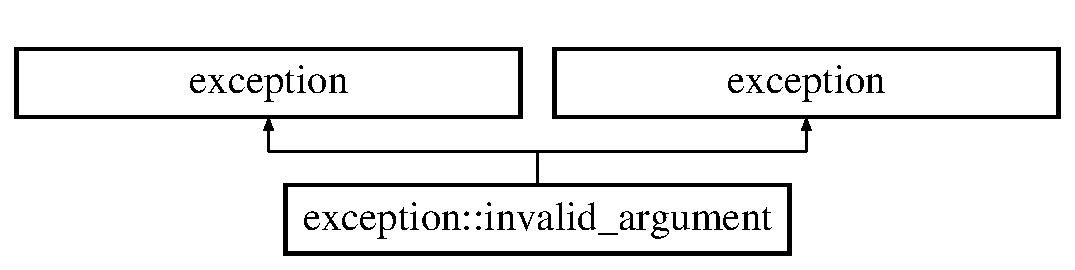
\includegraphics[height=2.000000cm]{classexception_1_1invalid__argument}
\end{center}
\end{figure}


\subsection{Detailed Description}


Definition at line 10 of file exception\+\_\+handling.\+hpp.



The documentation for this class was generated from the following file\+:\begin{DoxyCompactItemize}
\item 
D\+:/c++/block\+\_\+matrix-\/master/block\+\_\+matrix-\/master/include/\mbox{\hyperlink{include_2exception__handling_8hpp}{exception\+\_\+handling.\+hpp}}\end{DoxyCompactItemize}

\hypertarget{classexception_1_1invalid__index}{}\section{exception\+:\+:invalid\+\_\+index Class Reference}
\label{classexception_1_1invalid__index}\index{exception\+::invalid\+\_\+index@{exception\+::invalid\+\_\+index}}


{\ttfamily \#include $<$exception\+\_\+handling.\+hpp$>$}

Inheritance diagram for exception\+:\+:invalid\+\_\+index\+:\begin{figure}[H]
\begin{center}
\leavevmode
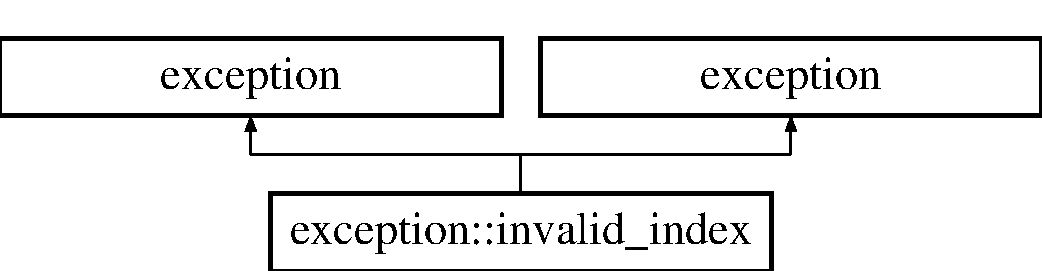
\includegraphics[height=2.000000cm]{classexception_1_1invalid__index}
\end{center}
\end{figure}


\subsection{Detailed Description}


Definition at line 18 of file exception\+\_\+handling.\+hpp.



The documentation for this class was generated from the following file\+:\begin{DoxyCompactItemize}
\item 
D\+:/c++/block\+\_\+matrix-\/master/block\+\_\+matrix-\/master/include/\mbox{\hyperlink{include_2exception__handling_8hpp}{exception\+\_\+handling.\+hpp}}\end{DoxyCompactItemize}

\hypertarget{classexception_1_1invalid__matrix}{}\section{exception\+:\+:invalid\+\_\+matrix Class Reference}
\label{classexception_1_1invalid__matrix}\index{exception\+::invalid\+\_\+matrix@{exception\+::invalid\+\_\+matrix}}


{\ttfamily \#include $<$exception\+\_\+handling.\+hpp$>$}

Inheritance diagram for exception\+:\+:invalid\+\_\+matrix\+:\begin{figure}[H]
\begin{center}
\leavevmode
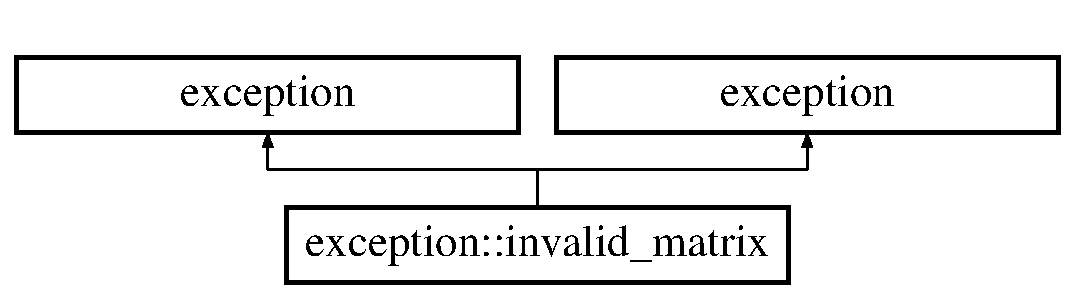
\includegraphics[height=2.000000cm]{classexception_1_1invalid__matrix}
\end{center}
\end{figure}


\subsection{Detailed Description}


Definition at line 26 of file exception\+\_\+handling.\+hpp.



The documentation for this class was generated from the following file\+:\begin{DoxyCompactItemize}
\item 
D\+:/c++/block\+\_\+matrix-\/master/block\+\_\+matrix-\/master/include/\mbox{\hyperlink{include_2exception__handling_8hpp}{exception\+\_\+handling.\+hpp}}\end{DoxyCompactItemize}

\hypertarget{classexception_1_1invalid__size}{}\section{exception\+:\+:invalid\+\_\+size Class Reference}
\label{classexception_1_1invalid__size}\index{exception\+::invalid\+\_\+size@{exception\+::invalid\+\_\+size}}


{\ttfamily \#include $<$exception\+\_\+handling.\+hpp$>$}

Inheritance diagram for exception\+:\+:invalid\+\_\+size\+:\begin{figure}[H]
\begin{center}
\leavevmode
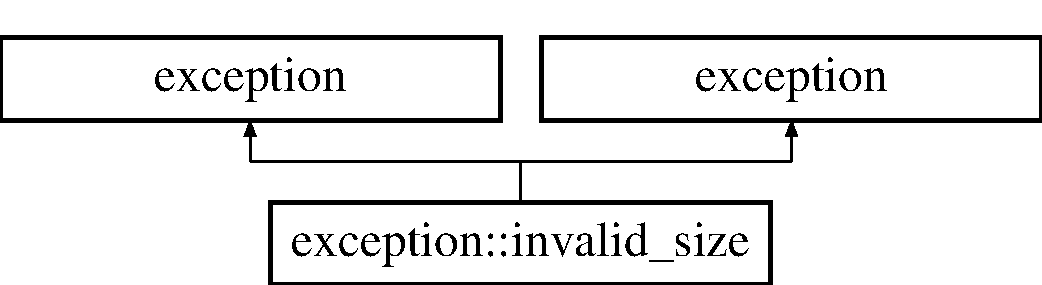
\includegraphics[height=2.000000cm]{classexception_1_1invalid__size}
\end{center}
\end{figure}


\subsection{Detailed Description}


Definition at line 34 of file exception\+\_\+handling.\+hpp.



The documentation for this class was generated from the following file\+:\begin{DoxyCompactItemize}
\item 
D\+:/c++/block\+\_\+matrix-\/master/block\+\_\+matrix-\/master/include/\mbox{\hyperlink{include_2exception__handling_8hpp}{exception\+\_\+handling.\+hpp}}\end{DoxyCompactItemize}

\hypertarget{struct_catch_1_1_i_registry_hub}{}\section{Catch\+:\+:I\+Registry\+Hub Struct Reference}
\label{struct_catch_1_1_i_registry_hub}\index{Catch\+::\+I\+Registry\+Hub@{Catch\+::\+I\+Registry\+Hub}}


{\ttfamily \#include $<$catch.\+hpp$>$}

\subsection*{Public Member Functions}
\begin{DoxyCompactItemize}
\item 
virtual \mbox{\hyperlink{struct_catch_1_1_i_registry_hub_a050de0f27f96888c8b410992146c9a09}{$\sim$\+I\+Registry\+Hub}} ()
\item 
virtual I\+Reporter\+Registry const  \& \mbox{\hyperlink{struct_catch_1_1_i_registry_hub_a55534563f7ecf7e20ec1e37285ebe54d}{get\+Reporter\+Registry}} () const =0
\item 
virtual \mbox{\hyperlink{struct_catch_1_1_i_test_case_registry}{I\+Test\+Case\+Registry}} const  \& \mbox{\hyperlink{struct_catch_1_1_i_registry_hub_af4f6255f0c0f8f1f179fa9d7d4843076}{get\+Test\+Case\+Registry}} () const =0
\item 
virtual I\+Tag\+Alias\+Registry const  \& \mbox{\hyperlink{struct_catch_1_1_i_registry_hub_a3c511b1d33e5a6d95c333a0ff387df1a}{get\+Tag\+Alias\+Registry}} () const =0
\item 
virtual \mbox{\hyperlink{struct_catch_1_1_i_exception_translator_registry}{I\+Exception\+Translator\+Registry}} \& \mbox{\hyperlink{struct_catch_1_1_i_registry_hub_a3606988da110c016c5af3ae63454eb78}{get\+Exception\+Translator\+Registry}} ()=0
\item 
virtual Startup\+Exception\+Registry const  \& \mbox{\hyperlink{struct_catch_1_1_i_registry_hub_a00281210628e6c616aca1d3e0d84db04}{get\+Startup\+Exception\+Registry}} () const =0
\end{DoxyCompactItemize}


\subsection{Detailed Description}


Definition at line 1916 of file catch.\+hpp.



\subsection{Constructor \& Destructor Documentation}
\mbox{\Hypertarget{struct_catch_1_1_i_registry_hub_a050de0f27f96888c8b410992146c9a09}\label{struct_catch_1_1_i_registry_hub_a050de0f27f96888c8b410992146c9a09}} 
\index{Catch\+::\+I\+Registry\+Hub@{Catch\+::\+I\+Registry\+Hub}!````~I\+Registry\+Hub@{$\sim$\+I\+Registry\+Hub}}
\index{````~I\+Registry\+Hub@{$\sim$\+I\+Registry\+Hub}!Catch\+::\+I\+Registry\+Hub@{Catch\+::\+I\+Registry\+Hub}}
\subsubsection{\texorpdfstring{$\sim$\+I\+Registry\+Hub()}{~IRegistryHub()}}
{\footnotesize\ttfamily virtual Catch\+::\+I\+Registry\+Hub\+::$\sim$\+I\+Registry\+Hub (\begin{DoxyParamCaption}{ }\end{DoxyParamCaption})\hspace{0.3cm}{\ttfamily [virtual]}}



\subsection{Member Function Documentation}
\mbox{\Hypertarget{struct_catch_1_1_i_registry_hub_a3606988da110c016c5af3ae63454eb78}\label{struct_catch_1_1_i_registry_hub_a3606988da110c016c5af3ae63454eb78}} 
\index{Catch\+::\+I\+Registry\+Hub@{Catch\+::\+I\+Registry\+Hub}!get\+Exception\+Translator\+Registry@{get\+Exception\+Translator\+Registry}}
\index{get\+Exception\+Translator\+Registry@{get\+Exception\+Translator\+Registry}!Catch\+::\+I\+Registry\+Hub@{Catch\+::\+I\+Registry\+Hub}}
\subsubsection{\texorpdfstring{get\+Exception\+Translator\+Registry()}{getExceptionTranslatorRegistry()}}
{\footnotesize\ttfamily virtual \mbox{\hyperlink{struct_catch_1_1_i_exception_translator_registry}{I\+Exception\+Translator\+Registry}}\& Catch\+::\+I\+Registry\+Hub\+::get\+Exception\+Translator\+Registry (\begin{DoxyParamCaption}{ }\end{DoxyParamCaption})\hspace{0.3cm}{\ttfamily [pure virtual]}}

\mbox{\Hypertarget{struct_catch_1_1_i_registry_hub_a55534563f7ecf7e20ec1e37285ebe54d}\label{struct_catch_1_1_i_registry_hub_a55534563f7ecf7e20ec1e37285ebe54d}} 
\index{Catch\+::\+I\+Registry\+Hub@{Catch\+::\+I\+Registry\+Hub}!get\+Reporter\+Registry@{get\+Reporter\+Registry}}
\index{get\+Reporter\+Registry@{get\+Reporter\+Registry}!Catch\+::\+I\+Registry\+Hub@{Catch\+::\+I\+Registry\+Hub}}
\subsubsection{\texorpdfstring{get\+Reporter\+Registry()}{getReporterRegistry()}}
{\footnotesize\ttfamily virtual I\+Reporter\+Registry const\& Catch\+::\+I\+Registry\+Hub\+::get\+Reporter\+Registry (\begin{DoxyParamCaption}{ }\end{DoxyParamCaption}) const\hspace{0.3cm}{\ttfamily [pure virtual]}}

\mbox{\Hypertarget{struct_catch_1_1_i_registry_hub_a00281210628e6c616aca1d3e0d84db04}\label{struct_catch_1_1_i_registry_hub_a00281210628e6c616aca1d3e0d84db04}} 
\index{Catch\+::\+I\+Registry\+Hub@{Catch\+::\+I\+Registry\+Hub}!get\+Startup\+Exception\+Registry@{get\+Startup\+Exception\+Registry}}
\index{get\+Startup\+Exception\+Registry@{get\+Startup\+Exception\+Registry}!Catch\+::\+I\+Registry\+Hub@{Catch\+::\+I\+Registry\+Hub}}
\subsubsection{\texorpdfstring{get\+Startup\+Exception\+Registry()}{getStartupExceptionRegistry()}}
{\footnotesize\ttfamily virtual Startup\+Exception\+Registry const\& Catch\+::\+I\+Registry\+Hub\+::get\+Startup\+Exception\+Registry (\begin{DoxyParamCaption}{ }\end{DoxyParamCaption}) const\hspace{0.3cm}{\ttfamily [pure virtual]}}

\mbox{\Hypertarget{struct_catch_1_1_i_registry_hub_a3c511b1d33e5a6d95c333a0ff387df1a}\label{struct_catch_1_1_i_registry_hub_a3c511b1d33e5a6d95c333a0ff387df1a}} 
\index{Catch\+::\+I\+Registry\+Hub@{Catch\+::\+I\+Registry\+Hub}!get\+Tag\+Alias\+Registry@{get\+Tag\+Alias\+Registry}}
\index{get\+Tag\+Alias\+Registry@{get\+Tag\+Alias\+Registry}!Catch\+::\+I\+Registry\+Hub@{Catch\+::\+I\+Registry\+Hub}}
\subsubsection{\texorpdfstring{get\+Tag\+Alias\+Registry()}{getTagAliasRegistry()}}
{\footnotesize\ttfamily virtual I\+Tag\+Alias\+Registry const\& Catch\+::\+I\+Registry\+Hub\+::get\+Tag\+Alias\+Registry (\begin{DoxyParamCaption}{ }\end{DoxyParamCaption}) const\hspace{0.3cm}{\ttfamily [pure virtual]}}

\mbox{\Hypertarget{struct_catch_1_1_i_registry_hub_af4f6255f0c0f8f1f179fa9d7d4843076}\label{struct_catch_1_1_i_registry_hub_af4f6255f0c0f8f1f179fa9d7d4843076}} 
\index{Catch\+::\+I\+Registry\+Hub@{Catch\+::\+I\+Registry\+Hub}!get\+Test\+Case\+Registry@{get\+Test\+Case\+Registry}}
\index{get\+Test\+Case\+Registry@{get\+Test\+Case\+Registry}!Catch\+::\+I\+Registry\+Hub@{Catch\+::\+I\+Registry\+Hub}}
\subsubsection{\texorpdfstring{get\+Test\+Case\+Registry()}{getTestCaseRegistry()}}
{\footnotesize\ttfamily virtual \mbox{\hyperlink{struct_catch_1_1_i_test_case_registry}{I\+Test\+Case\+Registry}} const\& Catch\+::\+I\+Registry\+Hub\+::get\+Test\+Case\+Registry (\begin{DoxyParamCaption}{ }\end{DoxyParamCaption}) const\hspace{0.3cm}{\ttfamily [pure virtual]}}



The documentation for this struct was generated from the following file\+:\begin{DoxyCompactItemize}
\item 
D\+:/c++/block\+\_\+matrix-\/master/block\+\_\+matrix-\/master/test/\mbox{\hyperlink{catch_8hpp}{catch.\+hpp}}\end{DoxyCompactItemize}

\hypertarget{struct_catch_1_1_i_result_capture}{}\section{Catch\+:\+:I\+Result\+Capture Struct Reference}
\label{struct_catch_1_1_i_result_capture}\index{Catch\+::\+I\+Result\+Capture@{Catch\+::\+I\+Result\+Capture}}


{\ttfamily \#include $<$catch.\+hpp$>$}

\subsection*{Public Member Functions}
\begin{DoxyCompactItemize}
\item 
virtual \mbox{\hyperlink{struct_catch_1_1_i_result_capture_a3bd16719d6772b7470887fc36c6d0808}{$\sim$\+I\+Result\+Capture}} ()
\item 
virtual bool \mbox{\hyperlink{struct_catch_1_1_i_result_capture_a5b76ed52badcb64cf374202e12b81a03}{section\+Started}} (\mbox{\hyperlink{struct_catch_1_1_section_info}{Section\+Info}} const \&section\+Info, \mbox{\hyperlink{struct_catch_1_1_counts}{Counts}} \&assertions)=0
\item 
virtual void \mbox{\hyperlink{struct_catch_1_1_i_result_capture_a4e152bc43dc0933684e31fa67a58195d}{section\+Ended}} (\mbox{\hyperlink{struct_catch_1_1_section_end_info}{Section\+End\+Info}} const \&end\+Info)=0
\item 
virtual void \mbox{\hyperlink{struct_catch_1_1_i_result_capture_afcc71eef8ca821ae132cced4a2be6988}{section\+Ended\+Early}} (\mbox{\hyperlink{struct_catch_1_1_section_end_info}{Section\+End\+Info}} const \&end\+Info)=0
\item 
virtual void \mbox{\hyperlink{struct_catch_1_1_i_result_capture_a264ae12330c74b2daae41715a30d51bf}{benchmark\+Starting}} (Benchmark\+Info const \&info)=0
\item 
virtual void \mbox{\hyperlink{struct_catch_1_1_i_result_capture_a6e5e64f9d94211a888249012ab6cc7fb}{benchmark\+Ended}} (Benchmark\+Stats const \&stats)=0
\item 
virtual void \mbox{\hyperlink{struct_catch_1_1_i_result_capture_a91d154c1e087e383dcde5aad95cb6a05}{push\+Scoped\+Message}} (\mbox{\hyperlink{struct_catch_1_1_message_info}{Message\+Info}} const \&message)=0
\item 
virtual void \mbox{\hyperlink{struct_catch_1_1_i_result_capture_a42bcb13276706bf8c3ce081ce16d37fd}{pop\+Scoped\+Message}} (\mbox{\hyperlink{struct_catch_1_1_message_info}{Message\+Info}} const \&message)=0
\item 
virtual void \mbox{\hyperlink{struct_catch_1_1_i_result_capture_a48559e6598ba9474b903697b69c769b2}{handle\+Fatal\+Error\+Condition}} (\mbox{\hyperlink{class_catch_1_1_string_ref}{String\+Ref}} message)=0
\item 
virtual void \mbox{\hyperlink{struct_catch_1_1_i_result_capture_a59a2b05391e464954575d2afb6d5d607}{handle\+Expr}} (\mbox{\hyperlink{struct_catch_1_1_assertion_info}{Assertion\+Info}} const \&info, \mbox{\hyperlink{struct_catch_1_1_i_transient_expression}{I\+Transient\+Expression}} const \&expr, \mbox{\hyperlink{struct_catch_1_1_assertion_reaction}{Assertion\+Reaction}} \&reaction)=0
\item 
virtual void \mbox{\hyperlink{struct_catch_1_1_i_result_capture_a21788ebc64571abf322b80c8cc51794d}{handle\+Message}} (\mbox{\hyperlink{struct_catch_1_1_assertion_info}{Assertion\+Info}} const \&info, \mbox{\hyperlink{struct_catch_1_1_result_was_a624e1ee3661fcf6094ceef1f654601ef}{Result\+Was\+::\+Of\+Type}} result\+Type, \mbox{\hyperlink{class_catch_1_1_string_ref}{String\+Ref}} const \&message, \mbox{\hyperlink{struct_catch_1_1_assertion_reaction}{Assertion\+Reaction}} \&reaction)=0
\item 
virtual void \mbox{\hyperlink{struct_catch_1_1_i_result_capture_a6382ed20486e2d9a020da971c6d5c53d}{handle\+Unexpected\+Exception\+Not\+Thrown}} (\mbox{\hyperlink{struct_catch_1_1_assertion_info}{Assertion\+Info}} const \&info, \mbox{\hyperlink{struct_catch_1_1_assertion_reaction}{Assertion\+Reaction}} \&reaction)=0
\item 
virtual void \mbox{\hyperlink{struct_catch_1_1_i_result_capture_afc97bc69829185222f955ebeef97adfe}{handle\+Unexpected\+Inflight\+Exception}} (\mbox{\hyperlink{struct_catch_1_1_assertion_info}{Assertion\+Info}} const \&info, std\+::string const \&message, \mbox{\hyperlink{struct_catch_1_1_assertion_reaction}{Assertion\+Reaction}} \&reaction)=0
\item 
virtual void \mbox{\hyperlink{struct_catch_1_1_i_result_capture_a89b89372eb09cc44f8dcad363de6157d}{handle\+Incomplete}} (\mbox{\hyperlink{struct_catch_1_1_assertion_info}{Assertion\+Info}} const \&info)=0
\item 
virtual void \mbox{\hyperlink{struct_catch_1_1_i_result_capture_ab7dbdf8aa28427119583e24dbb302c63}{handle\+Non\+Expr}} (\mbox{\hyperlink{struct_catch_1_1_assertion_info}{Assertion\+Info}} const \&info, \mbox{\hyperlink{struct_catch_1_1_result_was_a624e1ee3661fcf6094ceef1f654601ef}{Result\+Was\+::\+Of\+Type}} result\+Type, \mbox{\hyperlink{struct_catch_1_1_assertion_reaction}{Assertion\+Reaction}} \&reaction)=0
\item 
virtual bool \mbox{\hyperlink{struct_catch_1_1_i_result_capture_a973435fbdcb2f6f07a0ec5719a01e956}{last\+Assertion\+Passed}} ()=0
\item 
virtual void \mbox{\hyperlink{struct_catch_1_1_i_result_capture_a9b0ef2cb071e9a9dc6ec1b533026aea7}{assertion\+Passed}} ()=0
\item 
virtual std\+::string \mbox{\hyperlink{struct_catch_1_1_i_result_capture_aea1617f4a84cc648246aa3ed6918b5bf}{get\+Current\+Test\+Name}} () const =0
\item 
virtual const Assertion\+Result $\ast$ \mbox{\hyperlink{struct_catch_1_1_i_result_capture_ab18872c89fab97405a56e9c6a4919736}{get\+Last\+Result}} () const =0
\item 
virtual void \mbox{\hyperlink{struct_catch_1_1_i_result_capture_ae63ecec95db4c236c63ecf616f483810}{exception\+Early\+Reported}} ()=0
\end{DoxyCompactItemize}


\subsection{Detailed Description}


Definition at line 1421 of file catch.\+hpp.



\subsection{Constructor \& Destructor Documentation}
\mbox{\Hypertarget{struct_catch_1_1_i_result_capture_a3bd16719d6772b7470887fc36c6d0808}\label{struct_catch_1_1_i_result_capture_a3bd16719d6772b7470887fc36c6d0808}} 
\index{Catch\+::\+I\+Result\+Capture@{Catch\+::\+I\+Result\+Capture}!````~I\+Result\+Capture@{$\sim$\+I\+Result\+Capture}}
\index{````~I\+Result\+Capture@{$\sim$\+I\+Result\+Capture}!Catch\+::\+I\+Result\+Capture@{Catch\+::\+I\+Result\+Capture}}
\subsubsection{\texorpdfstring{$\sim$\+I\+Result\+Capture()}{~IResultCapture()}}
{\footnotesize\ttfamily virtual Catch\+::\+I\+Result\+Capture\+::$\sim$\+I\+Result\+Capture (\begin{DoxyParamCaption}{ }\end{DoxyParamCaption})\hspace{0.3cm}{\ttfamily [virtual]}}



\subsection{Member Function Documentation}
\mbox{\Hypertarget{struct_catch_1_1_i_result_capture_a9b0ef2cb071e9a9dc6ec1b533026aea7}\label{struct_catch_1_1_i_result_capture_a9b0ef2cb071e9a9dc6ec1b533026aea7}} 
\index{Catch\+::\+I\+Result\+Capture@{Catch\+::\+I\+Result\+Capture}!assertion\+Passed@{assertion\+Passed}}
\index{assertion\+Passed@{assertion\+Passed}!Catch\+::\+I\+Result\+Capture@{Catch\+::\+I\+Result\+Capture}}
\subsubsection{\texorpdfstring{assertion\+Passed()}{assertionPassed()}}
{\footnotesize\ttfamily virtual void Catch\+::\+I\+Result\+Capture\+::assertion\+Passed (\begin{DoxyParamCaption}{ }\end{DoxyParamCaption})\hspace{0.3cm}{\ttfamily [pure virtual]}}

\mbox{\Hypertarget{struct_catch_1_1_i_result_capture_a6e5e64f9d94211a888249012ab6cc7fb}\label{struct_catch_1_1_i_result_capture_a6e5e64f9d94211a888249012ab6cc7fb}} 
\index{Catch\+::\+I\+Result\+Capture@{Catch\+::\+I\+Result\+Capture}!benchmark\+Ended@{benchmark\+Ended}}
\index{benchmark\+Ended@{benchmark\+Ended}!Catch\+::\+I\+Result\+Capture@{Catch\+::\+I\+Result\+Capture}}
\subsubsection{\texorpdfstring{benchmark\+Ended()}{benchmarkEnded()}}
{\footnotesize\ttfamily virtual void Catch\+::\+I\+Result\+Capture\+::benchmark\+Ended (\begin{DoxyParamCaption}\item[{Benchmark\+Stats const \&}]{stats }\end{DoxyParamCaption})\hspace{0.3cm}{\ttfamily [pure virtual]}}

\mbox{\Hypertarget{struct_catch_1_1_i_result_capture_a264ae12330c74b2daae41715a30d51bf}\label{struct_catch_1_1_i_result_capture_a264ae12330c74b2daae41715a30d51bf}} 
\index{Catch\+::\+I\+Result\+Capture@{Catch\+::\+I\+Result\+Capture}!benchmark\+Starting@{benchmark\+Starting}}
\index{benchmark\+Starting@{benchmark\+Starting}!Catch\+::\+I\+Result\+Capture@{Catch\+::\+I\+Result\+Capture}}
\subsubsection{\texorpdfstring{benchmark\+Starting()}{benchmarkStarting()}}
{\footnotesize\ttfamily virtual void Catch\+::\+I\+Result\+Capture\+::benchmark\+Starting (\begin{DoxyParamCaption}\item[{Benchmark\+Info const \&}]{info }\end{DoxyParamCaption})\hspace{0.3cm}{\ttfamily [pure virtual]}}

\mbox{\Hypertarget{struct_catch_1_1_i_result_capture_ae63ecec95db4c236c63ecf616f483810}\label{struct_catch_1_1_i_result_capture_ae63ecec95db4c236c63ecf616f483810}} 
\index{Catch\+::\+I\+Result\+Capture@{Catch\+::\+I\+Result\+Capture}!exception\+Early\+Reported@{exception\+Early\+Reported}}
\index{exception\+Early\+Reported@{exception\+Early\+Reported}!Catch\+::\+I\+Result\+Capture@{Catch\+::\+I\+Result\+Capture}}
\subsubsection{\texorpdfstring{exception\+Early\+Reported()}{exceptionEarlyReported()}}
{\footnotesize\ttfamily virtual void Catch\+::\+I\+Result\+Capture\+::exception\+Early\+Reported (\begin{DoxyParamCaption}{ }\end{DoxyParamCaption})\hspace{0.3cm}{\ttfamily [pure virtual]}}

\mbox{\Hypertarget{struct_catch_1_1_i_result_capture_aea1617f4a84cc648246aa3ed6918b5bf}\label{struct_catch_1_1_i_result_capture_aea1617f4a84cc648246aa3ed6918b5bf}} 
\index{Catch\+::\+I\+Result\+Capture@{Catch\+::\+I\+Result\+Capture}!get\+Current\+Test\+Name@{get\+Current\+Test\+Name}}
\index{get\+Current\+Test\+Name@{get\+Current\+Test\+Name}!Catch\+::\+I\+Result\+Capture@{Catch\+::\+I\+Result\+Capture}}
\subsubsection{\texorpdfstring{get\+Current\+Test\+Name()}{getCurrentTestName()}}
{\footnotesize\ttfamily virtual std\+::string Catch\+::\+I\+Result\+Capture\+::get\+Current\+Test\+Name (\begin{DoxyParamCaption}{ }\end{DoxyParamCaption}) const\hspace{0.3cm}{\ttfamily [pure virtual]}}

\mbox{\Hypertarget{struct_catch_1_1_i_result_capture_ab18872c89fab97405a56e9c6a4919736}\label{struct_catch_1_1_i_result_capture_ab18872c89fab97405a56e9c6a4919736}} 
\index{Catch\+::\+I\+Result\+Capture@{Catch\+::\+I\+Result\+Capture}!get\+Last\+Result@{get\+Last\+Result}}
\index{get\+Last\+Result@{get\+Last\+Result}!Catch\+::\+I\+Result\+Capture@{Catch\+::\+I\+Result\+Capture}}
\subsubsection{\texorpdfstring{get\+Last\+Result()}{getLastResult()}}
{\footnotesize\ttfamily virtual const Assertion\+Result$\ast$ Catch\+::\+I\+Result\+Capture\+::get\+Last\+Result (\begin{DoxyParamCaption}{ }\end{DoxyParamCaption}) const\hspace{0.3cm}{\ttfamily [pure virtual]}}

\mbox{\Hypertarget{struct_catch_1_1_i_result_capture_a59a2b05391e464954575d2afb6d5d607}\label{struct_catch_1_1_i_result_capture_a59a2b05391e464954575d2afb6d5d607}} 
\index{Catch\+::\+I\+Result\+Capture@{Catch\+::\+I\+Result\+Capture}!handle\+Expr@{handle\+Expr}}
\index{handle\+Expr@{handle\+Expr}!Catch\+::\+I\+Result\+Capture@{Catch\+::\+I\+Result\+Capture}}
\subsubsection{\texorpdfstring{handle\+Expr()}{handleExpr()}}
{\footnotesize\ttfamily virtual void Catch\+::\+I\+Result\+Capture\+::handle\+Expr (\begin{DoxyParamCaption}\item[{\mbox{\hyperlink{struct_catch_1_1_assertion_info}{Assertion\+Info}} const \&}]{info,  }\item[{\mbox{\hyperlink{struct_catch_1_1_i_transient_expression}{I\+Transient\+Expression}} const \&}]{expr,  }\item[{\mbox{\hyperlink{struct_catch_1_1_assertion_reaction}{Assertion\+Reaction}} \&}]{reaction }\end{DoxyParamCaption})\hspace{0.3cm}{\ttfamily [pure virtual]}}

\mbox{\Hypertarget{struct_catch_1_1_i_result_capture_a48559e6598ba9474b903697b69c769b2}\label{struct_catch_1_1_i_result_capture_a48559e6598ba9474b903697b69c769b2}} 
\index{Catch\+::\+I\+Result\+Capture@{Catch\+::\+I\+Result\+Capture}!handle\+Fatal\+Error\+Condition@{handle\+Fatal\+Error\+Condition}}
\index{handle\+Fatal\+Error\+Condition@{handle\+Fatal\+Error\+Condition}!Catch\+::\+I\+Result\+Capture@{Catch\+::\+I\+Result\+Capture}}
\subsubsection{\texorpdfstring{handle\+Fatal\+Error\+Condition()}{handleFatalErrorCondition()}}
{\footnotesize\ttfamily virtual void Catch\+::\+I\+Result\+Capture\+::handle\+Fatal\+Error\+Condition (\begin{DoxyParamCaption}\item[{\mbox{\hyperlink{class_catch_1_1_string_ref}{String\+Ref}}}]{message }\end{DoxyParamCaption})\hspace{0.3cm}{\ttfamily [pure virtual]}}

\mbox{\Hypertarget{struct_catch_1_1_i_result_capture_a89b89372eb09cc44f8dcad363de6157d}\label{struct_catch_1_1_i_result_capture_a89b89372eb09cc44f8dcad363de6157d}} 
\index{Catch\+::\+I\+Result\+Capture@{Catch\+::\+I\+Result\+Capture}!handle\+Incomplete@{handle\+Incomplete}}
\index{handle\+Incomplete@{handle\+Incomplete}!Catch\+::\+I\+Result\+Capture@{Catch\+::\+I\+Result\+Capture}}
\subsubsection{\texorpdfstring{handle\+Incomplete()}{handleIncomplete()}}
{\footnotesize\ttfamily virtual void Catch\+::\+I\+Result\+Capture\+::handle\+Incomplete (\begin{DoxyParamCaption}\item[{\mbox{\hyperlink{struct_catch_1_1_assertion_info}{Assertion\+Info}} const \&}]{info }\end{DoxyParamCaption})\hspace{0.3cm}{\ttfamily [pure virtual]}}

\mbox{\Hypertarget{struct_catch_1_1_i_result_capture_a21788ebc64571abf322b80c8cc51794d}\label{struct_catch_1_1_i_result_capture_a21788ebc64571abf322b80c8cc51794d}} 
\index{Catch\+::\+I\+Result\+Capture@{Catch\+::\+I\+Result\+Capture}!handle\+Message@{handle\+Message}}
\index{handle\+Message@{handle\+Message}!Catch\+::\+I\+Result\+Capture@{Catch\+::\+I\+Result\+Capture}}
\subsubsection{\texorpdfstring{handle\+Message()}{handleMessage()}}
{\footnotesize\ttfamily virtual void Catch\+::\+I\+Result\+Capture\+::handle\+Message (\begin{DoxyParamCaption}\item[{\mbox{\hyperlink{struct_catch_1_1_assertion_info}{Assertion\+Info}} const \&}]{info,  }\item[{\mbox{\hyperlink{struct_catch_1_1_result_was_a624e1ee3661fcf6094ceef1f654601ef}{Result\+Was\+::\+Of\+Type}}}]{result\+Type,  }\item[{\mbox{\hyperlink{class_catch_1_1_string_ref}{String\+Ref}} const \&}]{message,  }\item[{\mbox{\hyperlink{struct_catch_1_1_assertion_reaction}{Assertion\+Reaction}} \&}]{reaction }\end{DoxyParamCaption})\hspace{0.3cm}{\ttfamily [pure virtual]}}

\mbox{\Hypertarget{struct_catch_1_1_i_result_capture_ab7dbdf8aa28427119583e24dbb302c63}\label{struct_catch_1_1_i_result_capture_ab7dbdf8aa28427119583e24dbb302c63}} 
\index{Catch\+::\+I\+Result\+Capture@{Catch\+::\+I\+Result\+Capture}!handle\+Non\+Expr@{handle\+Non\+Expr}}
\index{handle\+Non\+Expr@{handle\+Non\+Expr}!Catch\+::\+I\+Result\+Capture@{Catch\+::\+I\+Result\+Capture}}
\subsubsection{\texorpdfstring{handle\+Non\+Expr()}{handleNonExpr()}}
{\footnotesize\ttfamily virtual void Catch\+::\+I\+Result\+Capture\+::handle\+Non\+Expr (\begin{DoxyParamCaption}\item[{\mbox{\hyperlink{struct_catch_1_1_assertion_info}{Assertion\+Info}} const \&}]{info,  }\item[{\mbox{\hyperlink{struct_catch_1_1_result_was_a624e1ee3661fcf6094ceef1f654601ef}{Result\+Was\+::\+Of\+Type}}}]{result\+Type,  }\item[{\mbox{\hyperlink{struct_catch_1_1_assertion_reaction}{Assertion\+Reaction}} \&}]{reaction }\end{DoxyParamCaption})\hspace{0.3cm}{\ttfamily [pure virtual]}}

\mbox{\Hypertarget{struct_catch_1_1_i_result_capture_a6382ed20486e2d9a020da971c6d5c53d}\label{struct_catch_1_1_i_result_capture_a6382ed20486e2d9a020da971c6d5c53d}} 
\index{Catch\+::\+I\+Result\+Capture@{Catch\+::\+I\+Result\+Capture}!handle\+Unexpected\+Exception\+Not\+Thrown@{handle\+Unexpected\+Exception\+Not\+Thrown}}
\index{handle\+Unexpected\+Exception\+Not\+Thrown@{handle\+Unexpected\+Exception\+Not\+Thrown}!Catch\+::\+I\+Result\+Capture@{Catch\+::\+I\+Result\+Capture}}
\subsubsection{\texorpdfstring{handle\+Unexpected\+Exception\+Not\+Thrown()}{handleUnexpectedExceptionNotThrown()}}
{\footnotesize\ttfamily virtual void Catch\+::\+I\+Result\+Capture\+::handle\+Unexpected\+Exception\+Not\+Thrown (\begin{DoxyParamCaption}\item[{\mbox{\hyperlink{struct_catch_1_1_assertion_info}{Assertion\+Info}} const \&}]{info,  }\item[{\mbox{\hyperlink{struct_catch_1_1_assertion_reaction}{Assertion\+Reaction}} \&}]{reaction }\end{DoxyParamCaption})\hspace{0.3cm}{\ttfamily [pure virtual]}}

\mbox{\Hypertarget{struct_catch_1_1_i_result_capture_afc97bc69829185222f955ebeef97adfe}\label{struct_catch_1_1_i_result_capture_afc97bc69829185222f955ebeef97adfe}} 
\index{Catch\+::\+I\+Result\+Capture@{Catch\+::\+I\+Result\+Capture}!handle\+Unexpected\+Inflight\+Exception@{handle\+Unexpected\+Inflight\+Exception}}
\index{handle\+Unexpected\+Inflight\+Exception@{handle\+Unexpected\+Inflight\+Exception}!Catch\+::\+I\+Result\+Capture@{Catch\+::\+I\+Result\+Capture}}
\subsubsection{\texorpdfstring{handle\+Unexpected\+Inflight\+Exception()}{handleUnexpectedInflightException()}}
{\footnotesize\ttfamily virtual void Catch\+::\+I\+Result\+Capture\+::handle\+Unexpected\+Inflight\+Exception (\begin{DoxyParamCaption}\item[{\mbox{\hyperlink{struct_catch_1_1_assertion_info}{Assertion\+Info}} const \&}]{info,  }\item[{std\+::string const \&}]{message,  }\item[{\mbox{\hyperlink{struct_catch_1_1_assertion_reaction}{Assertion\+Reaction}} \&}]{reaction }\end{DoxyParamCaption})\hspace{0.3cm}{\ttfamily [pure virtual]}}

\mbox{\Hypertarget{struct_catch_1_1_i_result_capture_a973435fbdcb2f6f07a0ec5719a01e956}\label{struct_catch_1_1_i_result_capture_a973435fbdcb2f6f07a0ec5719a01e956}} 
\index{Catch\+::\+I\+Result\+Capture@{Catch\+::\+I\+Result\+Capture}!last\+Assertion\+Passed@{last\+Assertion\+Passed}}
\index{last\+Assertion\+Passed@{last\+Assertion\+Passed}!Catch\+::\+I\+Result\+Capture@{Catch\+::\+I\+Result\+Capture}}
\subsubsection{\texorpdfstring{last\+Assertion\+Passed()}{lastAssertionPassed()}}
{\footnotesize\ttfamily virtual bool Catch\+::\+I\+Result\+Capture\+::last\+Assertion\+Passed (\begin{DoxyParamCaption}{ }\end{DoxyParamCaption})\hspace{0.3cm}{\ttfamily [pure virtual]}}

\mbox{\Hypertarget{struct_catch_1_1_i_result_capture_a42bcb13276706bf8c3ce081ce16d37fd}\label{struct_catch_1_1_i_result_capture_a42bcb13276706bf8c3ce081ce16d37fd}} 
\index{Catch\+::\+I\+Result\+Capture@{Catch\+::\+I\+Result\+Capture}!pop\+Scoped\+Message@{pop\+Scoped\+Message}}
\index{pop\+Scoped\+Message@{pop\+Scoped\+Message}!Catch\+::\+I\+Result\+Capture@{Catch\+::\+I\+Result\+Capture}}
\subsubsection{\texorpdfstring{pop\+Scoped\+Message()}{popScopedMessage()}}
{\footnotesize\ttfamily virtual void Catch\+::\+I\+Result\+Capture\+::pop\+Scoped\+Message (\begin{DoxyParamCaption}\item[{\mbox{\hyperlink{struct_catch_1_1_message_info}{Message\+Info}} const \&}]{message }\end{DoxyParamCaption})\hspace{0.3cm}{\ttfamily [pure virtual]}}

\mbox{\Hypertarget{struct_catch_1_1_i_result_capture_a91d154c1e087e383dcde5aad95cb6a05}\label{struct_catch_1_1_i_result_capture_a91d154c1e087e383dcde5aad95cb6a05}} 
\index{Catch\+::\+I\+Result\+Capture@{Catch\+::\+I\+Result\+Capture}!push\+Scoped\+Message@{push\+Scoped\+Message}}
\index{push\+Scoped\+Message@{push\+Scoped\+Message}!Catch\+::\+I\+Result\+Capture@{Catch\+::\+I\+Result\+Capture}}
\subsubsection{\texorpdfstring{push\+Scoped\+Message()}{pushScopedMessage()}}
{\footnotesize\ttfamily virtual void Catch\+::\+I\+Result\+Capture\+::push\+Scoped\+Message (\begin{DoxyParamCaption}\item[{\mbox{\hyperlink{struct_catch_1_1_message_info}{Message\+Info}} const \&}]{message }\end{DoxyParamCaption})\hspace{0.3cm}{\ttfamily [pure virtual]}}

\mbox{\Hypertarget{struct_catch_1_1_i_result_capture_a4e152bc43dc0933684e31fa67a58195d}\label{struct_catch_1_1_i_result_capture_a4e152bc43dc0933684e31fa67a58195d}} 
\index{Catch\+::\+I\+Result\+Capture@{Catch\+::\+I\+Result\+Capture}!section\+Ended@{section\+Ended}}
\index{section\+Ended@{section\+Ended}!Catch\+::\+I\+Result\+Capture@{Catch\+::\+I\+Result\+Capture}}
\subsubsection{\texorpdfstring{section\+Ended()}{sectionEnded()}}
{\footnotesize\ttfamily virtual void Catch\+::\+I\+Result\+Capture\+::section\+Ended (\begin{DoxyParamCaption}\item[{\mbox{\hyperlink{struct_catch_1_1_section_end_info}{Section\+End\+Info}} const \&}]{end\+Info }\end{DoxyParamCaption})\hspace{0.3cm}{\ttfamily [pure virtual]}}

\mbox{\Hypertarget{struct_catch_1_1_i_result_capture_afcc71eef8ca821ae132cced4a2be6988}\label{struct_catch_1_1_i_result_capture_afcc71eef8ca821ae132cced4a2be6988}} 
\index{Catch\+::\+I\+Result\+Capture@{Catch\+::\+I\+Result\+Capture}!section\+Ended\+Early@{section\+Ended\+Early}}
\index{section\+Ended\+Early@{section\+Ended\+Early}!Catch\+::\+I\+Result\+Capture@{Catch\+::\+I\+Result\+Capture}}
\subsubsection{\texorpdfstring{section\+Ended\+Early()}{sectionEndedEarly()}}
{\footnotesize\ttfamily virtual void Catch\+::\+I\+Result\+Capture\+::section\+Ended\+Early (\begin{DoxyParamCaption}\item[{\mbox{\hyperlink{struct_catch_1_1_section_end_info}{Section\+End\+Info}} const \&}]{end\+Info }\end{DoxyParamCaption})\hspace{0.3cm}{\ttfamily [pure virtual]}}

\mbox{\Hypertarget{struct_catch_1_1_i_result_capture_a5b76ed52badcb64cf374202e12b81a03}\label{struct_catch_1_1_i_result_capture_a5b76ed52badcb64cf374202e12b81a03}} 
\index{Catch\+::\+I\+Result\+Capture@{Catch\+::\+I\+Result\+Capture}!section\+Started@{section\+Started}}
\index{section\+Started@{section\+Started}!Catch\+::\+I\+Result\+Capture@{Catch\+::\+I\+Result\+Capture}}
\subsubsection{\texorpdfstring{section\+Started()}{sectionStarted()}}
{\footnotesize\ttfamily virtual bool Catch\+::\+I\+Result\+Capture\+::section\+Started (\begin{DoxyParamCaption}\item[{\mbox{\hyperlink{struct_catch_1_1_section_info}{Section\+Info}} const \&}]{section\+Info,  }\item[{\mbox{\hyperlink{struct_catch_1_1_counts}{Counts}} \&}]{assertions }\end{DoxyParamCaption})\hspace{0.3cm}{\ttfamily [pure virtual]}}



The documentation for this struct was generated from the following file\+:\begin{DoxyCompactItemize}
\item 
D\+:/c++/block\+\_\+matrix-\/master/block\+\_\+matrix-\/master/test/\mbox{\hyperlink{catch_8hpp}{catch.\+hpp}}\end{DoxyCompactItemize}

\hypertarget{struct_catch_1_1_i_runner}{}\section{Catch\+:\+:I\+Runner Struct Reference}
\label{struct_catch_1_1_i_runner}\index{Catch\+::\+I\+Runner@{Catch\+::\+I\+Runner}}


{\ttfamily \#include $<$catch.\+hpp$>$}

\subsection*{Public Member Functions}
\begin{DoxyCompactItemize}
\item 
virtual \mbox{\hyperlink{struct_catch_1_1_i_runner_a5f539a88a7772d68de8a2e4028774209}{$\sim$\+I\+Runner}} ()
\item 
virtual bool \mbox{\hyperlink{struct_catch_1_1_i_runner_a03713202dd2e041e30b8030088ab0116}{aborting}} () const =0
\end{DoxyCompactItemize}


\subsection{Detailed Description}


Definition at line 2756 of file catch.\+hpp.



\subsection{Constructor \& Destructor Documentation}
\mbox{\Hypertarget{struct_catch_1_1_i_runner_a5f539a88a7772d68de8a2e4028774209}\label{struct_catch_1_1_i_runner_a5f539a88a7772d68de8a2e4028774209}} 
\index{Catch\+::\+I\+Runner@{Catch\+::\+I\+Runner}!````~I\+Runner@{$\sim$\+I\+Runner}}
\index{````~I\+Runner@{$\sim$\+I\+Runner}!Catch\+::\+I\+Runner@{Catch\+::\+I\+Runner}}
\subsubsection{\texorpdfstring{$\sim$\+I\+Runner()}{~IRunner()}}
{\footnotesize\ttfamily virtual Catch\+::\+I\+Runner\+::$\sim$\+I\+Runner (\begin{DoxyParamCaption}{ }\end{DoxyParamCaption})\hspace{0.3cm}{\ttfamily [virtual]}}



\subsection{Member Function Documentation}
\mbox{\Hypertarget{struct_catch_1_1_i_runner_a03713202dd2e041e30b8030088ab0116}\label{struct_catch_1_1_i_runner_a03713202dd2e041e30b8030088ab0116}} 
\index{Catch\+::\+I\+Runner@{Catch\+::\+I\+Runner}!aborting@{aborting}}
\index{aborting@{aborting}!Catch\+::\+I\+Runner@{Catch\+::\+I\+Runner}}
\subsubsection{\texorpdfstring{aborting()}{aborting()}}
{\footnotesize\ttfamily virtual bool Catch\+::\+I\+Runner\+::aborting (\begin{DoxyParamCaption}{ }\end{DoxyParamCaption}) const\hspace{0.3cm}{\ttfamily [pure virtual]}}



The documentation for this struct was generated from the following file\+:\begin{DoxyCompactItemize}
\item 
D\+:/c++/block\+\_\+matrix-\/master/block\+\_\+matrix-\/master/test/\mbox{\hyperlink{catch_8hpp}{catch.\+hpp}}\end{DoxyCompactItemize}

\hypertarget{struct_catch_1_1is__range}{}\section{Catch\+:\+:is\+\_\+range$<$ T $>$ Struct Template Reference}
\label{struct_catch_1_1is__range}\index{Catch\+::is\+\_\+range$<$ T $>$@{Catch\+::is\+\_\+range$<$ T $>$}}


{\ttfamily \#include $<$catch.\+hpp$>$}

\subsection*{Static Public Attributes}
\begin{DoxyCompactItemize}
\item 
static const bool \mbox{\hyperlink{struct_catch_1_1is__range_afaec39e819c3956829cbbd00feba11be}{value}}
\end{DoxyCompactItemize}


\subsection{Detailed Description}
\subsubsection*{template$<$typename T$>$\newline
struct Catch\+::is\+\_\+range$<$ T $>$}



Definition at line 1077 of file catch.\+hpp.



\subsection{Member Data Documentation}
\mbox{\Hypertarget{struct_catch_1_1is__range_afaec39e819c3956829cbbd00feba11be}\label{struct_catch_1_1is__range_afaec39e819c3956829cbbd00feba11be}} 
\index{Catch\+::is\+\_\+range@{Catch\+::is\+\_\+range}!value@{value}}
\index{value@{value}!Catch\+::is\+\_\+range@{Catch\+::is\+\_\+range}}
\subsubsection{\texorpdfstring{value}{value}}
{\footnotesize\ttfamily template$<$typename T $>$ \\
const bool \mbox{\hyperlink{struct_catch_1_1is__range}{Catch\+::is\+\_\+range}}$<$ T $>$\+::value\hspace{0.3cm}{\ttfamily [static]}}

{\bfseries Initial value\+:}
\begin{DoxyCode}
=
            !std::is\_same<decltype(begin(std::declval<T>())), not\_this\_one>::
      \mbox{\hyperlink{struct_catch_1_1is__range_afaec39e819c3956829cbbd00feba11be}{value}} &&
            !std::is\_same<decltype(\mbox{\hyperlink{namespace_catch_a71fef6a57614eb2d9751f8586ff6de6a}{end}}(std::declval<T>())), not\_this\_one>
      \mbox{\hyperlink{struct_catch_1_1is__range_afaec39e819c3956829cbbd00feba11be}{::value}}
\end{DoxyCode}


Definition at line 1078 of file catch.\+hpp.



The documentation for this struct was generated from the following file\+:\begin{DoxyCompactItemize}
\item 
D\+:/c++/block\+\_\+matrix-\/master/block\+\_\+matrix-\/master/test/\mbox{\hyperlink{catch_8hpp}{catch.\+hpp}}\end{DoxyCompactItemize}

\hypertarget{class_catch_1_1_detail_1_1_is_stream_insertable}{}\section{Catch\+:\+:Detail\+:\+:Is\+Stream\+Insertable$<$ T $>$ Class Template Reference}
\label{class_catch_1_1_detail_1_1_is_stream_insertable}\index{Catch\+::\+Detail\+::\+Is\+Stream\+Insertable$<$ T $>$@{Catch\+::\+Detail\+::\+Is\+Stream\+Insertable$<$ T $>$}}


{\ttfamily \#include $<$catch.\+hpp$>$}

\subsection*{Static Public Attributes}
\begin{DoxyCompactItemize}
\item 
static const bool \mbox{\hyperlink{class_catch_1_1_detail_1_1_is_stream_insertable_a42818b09ae5851126a70ee263769e309}{value}} = decltype(test$<$std\+::ostream, const T\&$>$(0))\+::value
\end{DoxyCompactItemize}


\subsection{Detailed Description}
\subsubsection*{template$<$typename T$>$\newline
class Catch\+::\+Detail\+::\+Is\+Stream\+Insertable$<$ T $>$}



Definition at line 757 of file catch.\+hpp.



\subsection{Member Data Documentation}
\mbox{\Hypertarget{class_catch_1_1_detail_1_1_is_stream_insertable_a42818b09ae5851126a70ee263769e309}\label{class_catch_1_1_detail_1_1_is_stream_insertable_a42818b09ae5851126a70ee263769e309}} 
\index{Catch\+::\+Detail\+::\+Is\+Stream\+Insertable@{Catch\+::\+Detail\+::\+Is\+Stream\+Insertable}!value@{value}}
\index{value@{value}!Catch\+::\+Detail\+::\+Is\+Stream\+Insertable@{Catch\+::\+Detail\+::\+Is\+Stream\+Insertable}}
\subsubsection{\texorpdfstring{value}{value}}
{\footnotesize\ttfamily template$<$typename T $>$ \\
const bool \mbox{\hyperlink{class_catch_1_1_detail_1_1_is_stream_insertable}{Catch\+::\+Detail\+::\+Is\+Stream\+Insertable}}$<$ T $>$\+::value = decltype(test$<$std\+::ostream, const T\&$>$(0))\+::value\hspace{0.3cm}{\ttfamily [static]}}



Definition at line 766 of file catch.\+hpp.



The documentation for this class was generated from the following file\+:\begin{DoxyCompactItemize}
\item 
D\+:/c++/block\+\_\+matrix-\/master/block\+\_\+matrix-\/master/test/\mbox{\hyperlink{catch_8hpp}{catch.\+hpp}}\end{DoxyCompactItemize}

\hypertarget{struct_catch_1_1_i_stream}{}\section{Catch\+:\+:I\+Stream Struct Reference}
\label{struct_catch_1_1_i_stream}\index{Catch\+::\+I\+Stream@{Catch\+::\+I\+Stream}}


{\ttfamily \#include $<$catch.\+hpp$>$}

\subsection*{Public Member Functions}
\begin{DoxyCompactItemize}
\item 
virtual \mbox{\hyperlink{struct_catch_1_1_i_stream_a344a88d0e5fc1f727f5801c72b4a4e2a}{$\sim$\+I\+Stream}} ()
\item 
virtual std\+::ostream \& \mbox{\hyperlink{struct_catch_1_1_i_stream_a55a9ddbe250261ff38642f480ebdd902}{stream}} () const =0
\end{DoxyCompactItemize}


\subsection{Detailed Description}


Definition at line 657 of file catch.\+hpp.



\subsection{Constructor \& Destructor Documentation}
\mbox{\Hypertarget{struct_catch_1_1_i_stream_a344a88d0e5fc1f727f5801c72b4a4e2a}\label{struct_catch_1_1_i_stream_a344a88d0e5fc1f727f5801c72b4a4e2a}} 
\index{Catch\+::\+I\+Stream@{Catch\+::\+I\+Stream}!````~I\+Stream@{$\sim$\+I\+Stream}}
\index{````~I\+Stream@{$\sim$\+I\+Stream}!Catch\+::\+I\+Stream@{Catch\+::\+I\+Stream}}
\subsubsection{\texorpdfstring{$\sim$\+I\+Stream()}{~IStream()}}
{\footnotesize\ttfamily virtual Catch\+::\+I\+Stream\+::$\sim$\+I\+Stream (\begin{DoxyParamCaption}{ }\end{DoxyParamCaption})\hspace{0.3cm}{\ttfamily [virtual]}}



\subsection{Member Function Documentation}
\mbox{\Hypertarget{struct_catch_1_1_i_stream_a55a9ddbe250261ff38642f480ebdd902}\label{struct_catch_1_1_i_stream_a55a9ddbe250261ff38642f480ebdd902}} 
\index{Catch\+::\+I\+Stream@{Catch\+::\+I\+Stream}!stream@{stream}}
\index{stream@{stream}!Catch\+::\+I\+Stream@{Catch\+::\+I\+Stream}}
\subsubsection{\texorpdfstring{stream()}{stream()}}
{\footnotesize\ttfamily virtual std\+::ostream\& Catch\+::\+I\+Stream\+::stream (\begin{DoxyParamCaption}{ }\end{DoxyParamCaption}) const\hspace{0.3cm}{\ttfamily [pure virtual]}}



The documentation for this struct was generated from the following file\+:\begin{DoxyCompactItemize}
\item 
D\+:/c++/block\+\_\+matrix-\/master/block\+\_\+matrix-\/master/test/\mbox{\hyperlink{catch_8hpp}{catch.\+hpp}}\end{DoxyCompactItemize}

\hypertarget{struct_catch_1_1_i_test_case_registry}{}\section{Catch\+:\+:I\+Test\+Case\+Registry Struct Reference}
\label{struct_catch_1_1_i_test_case_registry}\index{Catch\+::\+I\+Test\+Case\+Registry@{Catch\+::\+I\+Test\+Case\+Registry}}


{\ttfamily \#include $<$catch.\+hpp$>$}

\subsection*{Public Member Functions}
\begin{DoxyCompactItemize}
\item 
virtual \mbox{\hyperlink{struct_catch_1_1_i_test_case_registry_ae14798f05ac8e2b18cff532849a4da81}{$\sim$\+I\+Test\+Case\+Registry}} ()
\item 
virtual std\+::vector$<$ \mbox{\hyperlink{class_catch_1_1_test_case}{Test\+Case}} $>$ const  \& \mbox{\hyperlink{struct_catch_1_1_i_test_case_registry_ad6e4d4a621655123f73ae98cfeda063d}{get\+All\+Tests}} () const =0
\item 
virtual std\+::vector$<$ \mbox{\hyperlink{class_catch_1_1_test_case}{Test\+Case}} $>$ const  \& \mbox{\hyperlink{struct_catch_1_1_i_test_case_registry_a33e46639d0319d35497c05bb5d02be5a}{get\+All\+Tests\+Sorted}} (I\+Config const \&config) const =0
\end{DoxyCompactItemize}


\subsection{Detailed Description}


Definition at line 347 of file catch.\+hpp.



\subsection{Constructor \& Destructor Documentation}
\mbox{\Hypertarget{struct_catch_1_1_i_test_case_registry_ae14798f05ac8e2b18cff532849a4da81}\label{struct_catch_1_1_i_test_case_registry_ae14798f05ac8e2b18cff532849a4da81}} 
\index{Catch\+::\+I\+Test\+Case\+Registry@{Catch\+::\+I\+Test\+Case\+Registry}!````~I\+Test\+Case\+Registry@{$\sim$\+I\+Test\+Case\+Registry}}
\index{````~I\+Test\+Case\+Registry@{$\sim$\+I\+Test\+Case\+Registry}!Catch\+::\+I\+Test\+Case\+Registry@{Catch\+::\+I\+Test\+Case\+Registry}}
\subsubsection{\texorpdfstring{$\sim$\+I\+Test\+Case\+Registry()}{~ITestCaseRegistry()}}
{\footnotesize\ttfamily virtual Catch\+::\+I\+Test\+Case\+Registry\+::$\sim$\+I\+Test\+Case\+Registry (\begin{DoxyParamCaption}{ }\end{DoxyParamCaption})\hspace{0.3cm}{\ttfamily [virtual]}}



\subsection{Member Function Documentation}
\mbox{\Hypertarget{struct_catch_1_1_i_test_case_registry_ad6e4d4a621655123f73ae98cfeda063d}\label{struct_catch_1_1_i_test_case_registry_ad6e4d4a621655123f73ae98cfeda063d}} 
\index{Catch\+::\+I\+Test\+Case\+Registry@{Catch\+::\+I\+Test\+Case\+Registry}!get\+All\+Tests@{get\+All\+Tests}}
\index{get\+All\+Tests@{get\+All\+Tests}!Catch\+::\+I\+Test\+Case\+Registry@{Catch\+::\+I\+Test\+Case\+Registry}}
\subsubsection{\texorpdfstring{get\+All\+Tests()}{getAllTests()}}
{\footnotesize\ttfamily virtual std\+::vector$<$\mbox{\hyperlink{class_catch_1_1_test_case}{Test\+Case}}$>$ const\& Catch\+::\+I\+Test\+Case\+Registry\+::get\+All\+Tests (\begin{DoxyParamCaption}{ }\end{DoxyParamCaption}) const\hspace{0.3cm}{\ttfamily [pure virtual]}}

\mbox{\Hypertarget{struct_catch_1_1_i_test_case_registry_a33e46639d0319d35497c05bb5d02be5a}\label{struct_catch_1_1_i_test_case_registry_a33e46639d0319d35497c05bb5d02be5a}} 
\index{Catch\+::\+I\+Test\+Case\+Registry@{Catch\+::\+I\+Test\+Case\+Registry}!get\+All\+Tests\+Sorted@{get\+All\+Tests\+Sorted}}
\index{get\+All\+Tests\+Sorted@{get\+All\+Tests\+Sorted}!Catch\+::\+I\+Test\+Case\+Registry@{Catch\+::\+I\+Test\+Case\+Registry}}
\subsubsection{\texorpdfstring{get\+All\+Tests\+Sorted()}{getAllTestsSorted()}}
{\footnotesize\ttfamily virtual std\+::vector$<$\mbox{\hyperlink{class_catch_1_1_test_case}{Test\+Case}}$>$ const\& Catch\+::\+I\+Test\+Case\+Registry\+::get\+All\+Tests\+Sorted (\begin{DoxyParamCaption}\item[{I\+Config const \&}]{config }\end{DoxyParamCaption}) const\hspace{0.3cm}{\ttfamily [pure virtual]}}



The documentation for this struct was generated from the following file\+:\begin{DoxyCompactItemize}
\item 
D\+:/c++/block\+\_\+matrix-\/master/block\+\_\+matrix-\/master/test/\mbox{\hyperlink{catch_8hpp}{catch.\+hpp}}\end{DoxyCompactItemize}

\hypertarget{struct_catch_1_1_i_test_invoker}{}\section{Catch\+:\+:I\+Test\+Invoker Struct Reference}
\label{struct_catch_1_1_i_test_invoker}\index{Catch\+::\+I\+Test\+Invoker@{Catch\+::\+I\+Test\+Invoker}}


{\ttfamily \#include $<$catch.\+hpp$>$}

Inheritance diagram for Catch\+:\+:I\+Test\+Invoker\+:\begin{figure}[H]
\begin{center}
\leavevmode
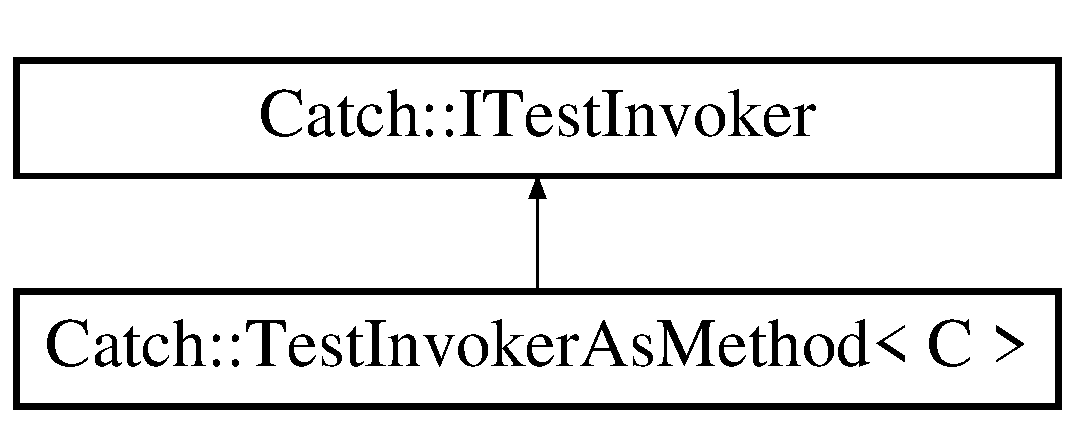
\includegraphics[height=2.000000cm]{struct_catch_1_1_i_test_invoker}
\end{center}
\end{figure}
\subsection*{Public Member Functions}
\begin{DoxyCompactItemize}
\item 
virtual void \mbox{\hyperlink{struct_catch_1_1_i_test_invoker_a6fcd5c5b67d6d5ade6491ff33411ca7f}{invoke}} () const =0
\item 
virtual \mbox{\hyperlink{struct_catch_1_1_i_test_invoker_a2c89f3eece5b1b677243766e409bd831}{$\sim$\+I\+Test\+Invoker}} ()
\end{DoxyCompactItemize}


\subsection{Detailed Description}


Definition at line 337 of file catch.\+hpp.



\subsection{Constructor \& Destructor Documentation}
\mbox{\Hypertarget{struct_catch_1_1_i_test_invoker_a2c89f3eece5b1b677243766e409bd831}\label{struct_catch_1_1_i_test_invoker_a2c89f3eece5b1b677243766e409bd831}} 
\index{Catch\+::\+I\+Test\+Invoker@{Catch\+::\+I\+Test\+Invoker}!````~I\+Test\+Invoker@{$\sim$\+I\+Test\+Invoker}}
\index{````~I\+Test\+Invoker@{$\sim$\+I\+Test\+Invoker}!Catch\+::\+I\+Test\+Invoker@{Catch\+::\+I\+Test\+Invoker}}
\subsubsection{\texorpdfstring{$\sim$\+I\+Test\+Invoker()}{~ITestInvoker()}}
{\footnotesize\ttfamily virtual Catch\+::\+I\+Test\+Invoker\+::$\sim$\+I\+Test\+Invoker (\begin{DoxyParamCaption}{ }\end{DoxyParamCaption})\hspace{0.3cm}{\ttfamily [virtual]}}



\subsection{Member Function Documentation}
\mbox{\Hypertarget{struct_catch_1_1_i_test_invoker_a6fcd5c5b67d6d5ade6491ff33411ca7f}\label{struct_catch_1_1_i_test_invoker_a6fcd5c5b67d6d5ade6491ff33411ca7f}} 
\index{Catch\+::\+I\+Test\+Invoker@{Catch\+::\+I\+Test\+Invoker}!invoke@{invoke}}
\index{invoke@{invoke}!Catch\+::\+I\+Test\+Invoker@{Catch\+::\+I\+Test\+Invoker}}
\subsubsection{\texorpdfstring{invoke()}{invoke()}}
{\footnotesize\ttfamily virtual void Catch\+::\+I\+Test\+Invoker\+::invoke (\begin{DoxyParamCaption}{ }\end{DoxyParamCaption}) const\hspace{0.3cm}{\ttfamily [pure virtual]}}



Implemented in \mbox{\hyperlink{class_catch_1_1_test_invoker_as_method_a8115a06efe273f4112ec0b5452c1b5f2}{Catch\+::\+Test\+Invoker\+As\+Method$<$ C $>$}}.



The documentation for this struct was generated from the following file\+:\begin{DoxyCompactItemize}
\item 
D\+:/c++/block\+\_\+matrix-\/master/block\+\_\+matrix-\/master/test/\mbox{\hyperlink{catch_8hpp}{catch.\+hpp}}\end{DoxyCompactItemize}

\hypertarget{struct_catch_1_1_i_transient_expression}{}\section{Catch\+:\+:I\+Transient\+Expression Struct Reference}
\label{struct_catch_1_1_i_transient_expression}\index{Catch\+::\+I\+Transient\+Expression@{Catch\+::\+I\+Transient\+Expression}}


{\ttfamily \#include $<$catch.\+hpp$>$}

Inheritance diagram for Catch\+:\+:I\+Transient\+Expression\+:\begin{figure}[H]
\begin{center}
\leavevmode
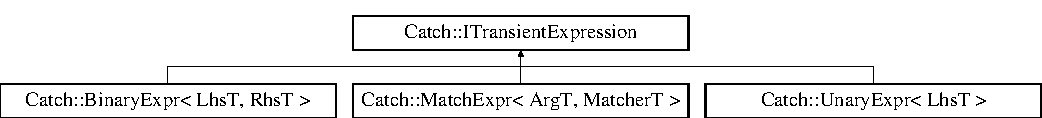
\includegraphics[height=1.588652cm]{struct_catch_1_1_i_transient_expression}
\end{center}
\end{figure}
\subsection*{Public Member Functions}
\begin{DoxyCompactItemize}
\item 
auto \mbox{\hyperlink{struct_catch_1_1_i_transient_expression_a3b436e13a0a6d3522bbf70d4e31deb22}{is\+Binary\+Expression}} () const -\/$>$ bool
\item 
auto \mbox{\hyperlink{struct_catch_1_1_i_transient_expression_a101c7db86c87eff93a8ff496720e6320}{get\+Result}} () const -\/$>$ bool
\item 
virtual void \mbox{\hyperlink{struct_catch_1_1_i_transient_expression_aabe1889df9c6e639a24afb08d8a0fe9e}{stream\+Reconstructed\+Expression}} (std\+::ostream \&os) const =0
\item 
\mbox{\hyperlink{struct_catch_1_1_i_transient_expression_aafe69572b7ed884e63ec81f58d4afd8c}{I\+Transient\+Expression}} (bool \mbox{\hyperlink{struct_catch_1_1_i_transient_expression_a3b436e13a0a6d3522bbf70d4e31deb22}{is\+Binary\+Expression}}, bool result)
\item 
virtual \mbox{\hyperlink{struct_catch_1_1_i_transient_expression_aeadf426de589938c4964fe4068eeee77}{$\sim$\+I\+Transient\+Expression}} ()
\end{DoxyCompactItemize}
\subsection*{Public Attributes}
\begin{DoxyCompactItemize}
\item 
bool \mbox{\hyperlink{struct_catch_1_1_i_transient_expression_a75ce48da824d514d08152d396abb28d8}{m\+\_\+is\+Binary\+Expression}}
\item 
bool \mbox{\hyperlink{struct_catch_1_1_i_transient_expression_a4646e2b5e0156e913653ec3b9b60c942}{m\+\_\+result}}
\end{DoxyCompactItemize}


\subsection{Detailed Description}


Definition at line 1255 of file catch.\+hpp.



\subsection{Constructor \& Destructor Documentation}
\mbox{\Hypertarget{struct_catch_1_1_i_transient_expression_aafe69572b7ed884e63ec81f58d4afd8c}\label{struct_catch_1_1_i_transient_expression_aafe69572b7ed884e63ec81f58d4afd8c}} 
\index{Catch\+::\+I\+Transient\+Expression@{Catch\+::\+I\+Transient\+Expression}!I\+Transient\+Expression@{I\+Transient\+Expression}}
\index{I\+Transient\+Expression@{I\+Transient\+Expression}!Catch\+::\+I\+Transient\+Expression@{Catch\+::\+I\+Transient\+Expression}}
\subsubsection{\texorpdfstring{I\+Transient\+Expression()}{ITransientExpression()}}
{\footnotesize\ttfamily Catch\+::\+I\+Transient\+Expression\+::\+I\+Transient\+Expression (\begin{DoxyParamCaption}\item[{bool}]{is\+Binary\+Expression,  }\item[{bool}]{result }\end{DoxyParamCaption})\hspace{0.3cm}{\ttfamily [inline]}}



Definition at line 1260 of file catch.\+hpp.

\mbox{\Hypertarget{struct_catch_1_1_i_transient_expression_aeadf426de589938c4964fe4068eeee77}\label{struct_catch_1_1_i_transient_expression_aeadf426de589938c4964fe4068eeee77}} 
\index{Catch\+::\+I\+Transient\+Expression@{Catch\+::\+I\+Transient\+Expression}!````~I\+Transient\+Expression@{$\sim$\+I\+Transient\+Expression}}
\index{````~I\+Transient\+Expression@{$\sim$\+I\+Transient\+Expression}!Catch\+::\+I\+Transient\+Expression@{Catch\+::\+I\+Transient\+Expression}}
\subsubsection{\texorpdfstring{$\sim$\+I\+Transient\+Expression()}{~ITransientExpression()}}
{\footnotesize\ttfamily virtual Catch\+::\+I\+Transient\+Expression\+::$\sim$\+I\+Transient\+Expression (\begin{DoxyParamCaption}{ }\end{DoxyParamCaption})\hspace{0.3cm}{\ttfamily [virtual]}}



\subsection{Member Function Documentation}
\mbox{\Hypertarget{struct_catch_1_1_i_transient_expression_a101c7db86c87eff93a8ff496720e6320}\label{struct_catch_1_1_i_transient_expression_a101c7db86c87eff93a8ff496720e6320}} 
\index{Catch\+::\+I\+Transient\+Expression@{Catch\+::\+I\+Transient\+Expression}!get\+Result@{get\+Result}}
\index{get\+Result@{get\+Result}!Catch\+::\+I\+Transient\+Expression@{Catch\+::\+I\+Transient\+Expression}}
\subsubsection{\texorpdfstring{get\+Result()}{getResult()}}
{\footnotesize\ttfamily auto Catch\+::\+I\+Transient\+Expression\+::get\+Result (\begin{DoxyParamCaption}{ }\end{DoxyParamCaption}) const -\/$>$ bool \hspace{0.3cm}{\ttfamily [inline]}}



Definition at line 1257 of file catch.\+hpp.

\mbox{\Hypertarget{struct_catch_1_1_i_transient_expression_a3b436e13a0a6d3522bbf70d4e31deb22}\label{struct_catch_1_1_i_transient_expression_a3b436e13a0a6d3522bbf70d4e31deb22}} 
\index{Catch\+::\+I\+Transient\+Expression@{Catch\+::\+I\+Transient\+Expression}!is\+Binary\+Expression@{is\+Binary\+Expression}}
\index{is\+Binary\+Expression@{is\+Binary\+Expression}!Catch\+::\+I\+Transient\+Expression@{Catch\+::\+I\+Transient\+Expression}}
\subsubsection{\texorpdfstring{is\+Binary\+Expression()}{isBinaryExpression()}}
{\footnotesize\ttfamily auto Catch\+::\+I\+Transient\+Expression\+::is\+Binary\+Expression (\begin{DoxyParamCaption}{ }\end{DoxyParamCaption}) const -\/$>$ bool \hspace{0.3cm}{\ttfamily [inline]}}



Definition at line 1256 of file catch.\+hpp.

\mbox{\Hypertarget{struct_catch_1_1_i_transient_expression_aabe1889df9c6e639a24afb08d8a0fe9e}\label{struct_catch_1_1_i_transient_expression_aabe1889df9c6e639a24afb08d8a0fe9e}} 
\index{Catch\+::\+I\+Transient\+Expression@{Catch\+::\+I\+Transient\+Expression}!stream\+Reconstructed\+Expression@{stream\+Reconstructed\+Expression}}
\index{stream\+Reconstructed\+Expression@{stream\+Reconstructed\+Expression}!Catch\+::\+I\+Transient\+Expression@{Catch\+::\+I\+Transient\+Expression}}
\subsubsection{\texorpdfstring{stream\+Reconstructed\+Expression()}{streamReconstructedExpression()}}
{\footnotesize\ttfamily virtual void Catch\+::\+I\+Transient\+Expression\+::stream\+Reconstructed\+Expression (\begin{DoxyParamCaption}\item[{std\+::ostream \&}]{os }\end{DoxyParamCaption}) const\hspace{0.3cm}{\ttfamily [pure virtual]}}



Implemented in \mbox{\hyperlink{class_catch_1_1_match_expr_ad3e41adb597750b2219bb37e51185629}{Catch\+::\+Match\+Expr$<$ Arg\+T, Matcher\+T $>$}}.



\subsection{Member Data Documentation}
\mbox{\Hypertarget{struct_catch_1_1_i_transient_expression_a75ce48da824d514d08152d396abb28d8}\label{struct_catch_1_1_i_transient_expression_a75ce48da824d514d08152d396abb28d8}} 
\index{Catch\+::\+I\+Transient\+Expression@{Catch\+::\+I\+Transient\+Expression}!m\+\_\+is\+Binary\+Expression@{m\+\_\+is\+Binary\+Expression}}
\index{m\+\_\+is\+Binary\+Expression@{m\+\_\+is\+Binary\+Expression}!Catch\+::\+I\+Transient\+Expression@{Catch\+::\+I\+Transient\+Expression}}
\subsubsection{\texorpdfstring{m\+\_\+is\+Binary\+Expression}{m\_isBinaryExpression}}
{\footnotesize\ttfamily bool Catch\+::\+I\+Transient\+Expression\+::m\+\_\+is\+Binary\+Expression}



Definition at line 1269 of file catch.\+hpp.

\mbox{\Hypertarget{struct_catch_1_1_i_transient_expression_a4646e2b5e0156e913653ec3b9b60c942}\label{struct_catch_1_1_i_transient_expression_a4646e2b5e0156e913653ec3b9b60c942}} 
\index{Catch\+::\+I\+Transient\+Expression@{Catch\+::\+I\+Transient\+Expression}!m\+\_\+result@{m\+\_\+result}}
\index{m\+\_\+result@{m\+\_\+result}!Catch\+::\+I\+Transient\+Expression@{Catch\+::\+I\+Transient\+Expression}}
\subsubsection{\texorpdfstring{m\+\_\+result}{m\_result}}
{\footnotesize\ttfamily bool Catch\+::\+I\+Transient\+Expression\+::m\+\_\+result}



Definition at line 1270 of file catch.\+hpp.



The documentation for this struct was generated from the following file\+:\begin{DoxyCompactItemize}
\item 
D\+:/c++/block\+\_\+matrix-\/master/block\+\_\+matrix-\/master/test/\mbox{\hyperlink{catch_8hpp}{catch.\+hpp}}\end{DoxyCompactItemize}

\hypertarget{class_catch_1_1_lazy_expression}{}\section{Catch\+:\+:Lazy\+Expression Class Reference}
\label{class_catch_1_1_lazy_expression}\index{Catch\+::\+Lazy\+Expression@{Catch\+::\+Lazy\+Expression}}


{\ttfamily \#include $<$catch.\+hpp$>$}

\subsection*{Public Member Functions}
\begin{DoxyCompactItemize}
\item 
\mbox{\hyperlink{class_catch_1_1_lazy_expression_a47186c2487bd4bf871e870ba8048553a}{Lazy\+Expression}} (bool is\+Negated)
\item 
\mbox{\hyperlink{class_catch_1_1_lazy_expression_ab82d5e94df0e159b018fbde0170e46f8}{Lazy\+Expression}} (\mbox{\hyperlink{class_catch_1_1_lazy_expression}{Lazy\+Expression}} const \&other)
\item 
\mbox{\hyperlink{class_catch_1_1_lazy_expression}{Lazy\+Expression}} \& \mbox{\hyperlink{class_catch_1_1_lazy_expression_ae4ae00d4f36f084c369f2da36565a822}{operator=}} (\mbox{\hyperlink{class_catch_1_1_lazy_expression}{Lazy\+Expression}} const \&)=delete
\item 
\mbox{\hyperlink{class_catch_1_1_lazy_expression_acdb846cb230cecfc6aca7a925b31fbca}{operator bool}} () const
\end{DoxyCompactItemize}
\subsection*{Friends}
\begin{DoxyCompactItemize}
\item 
class \mbox{\hyperlink{class_catch_1_1_lazy_expression_a4301a3aa57b612dd8b6ef8461742ecab}{Assertion\+Handler}}
\item 
struct \mbox{\hyperlink{class_catch_1_1_lazy_expression_a64019eb137f5ce447cdc71cb80b6e7a4}{Assertion\+Stats}}
\item 
class \mbox{\hyperlink{class_catch_1_1_lazy_expression_af3aa096bb29a772bc534830f29a2ce7a}{Run\+Context}}
\item 
auto \mbox{\hyperlink{class_catch_1_1_lazy_expression_aa01086581cab2fcd2d4580b8fa787dfc}{operator$<$$<$}} (std\+::ostream \&os, \mbox{\hyperlink{class_catch_1_1_lazy_expression}{Lazy\+Expression}} const \&lazy\+Expr) -\/$>$ std\+::ostream \&
\end{DoxyCompactItemize}


\subsection{Detailed Description}


Definition at line 1481 of file catch.\+hpp.



\subsection{Constructor \& Destructor Documentation}
\mbox{\Hypertarget{class_catch_1_1_lazy_expression_a47186c2487bd4bf871e870ba8048553a}\label{class_catch_1_1_lazy_expression_a47186c2487bd4bf871e870ba8048553a}} 
\index{Catch\+::\+Lazy\+Expression@{Catch\+::\+Lazy\+Expression}!Lazy\+Expression@{Lazy\+Expression}}
\index{Lazy\+Expression@{Lazy\+Expression}!Catch\+::\+Lazy\+Expression@{Catch\+::\+Lazy\+Expression}}
\subsubsection{\texorpdfstring{Lazy\+Expression()}{LazyExpression()}\hspace{0.1cm}{\footnotesize\ttfamily [1/2]}}
{\footnotesize\ttfamily Catch\+::\+Lazy\+Expression\+::\+Lazy\+Expression (\begin{DoxyParamCaption}\item[{bool}]{is\+Negated }\end{DoxyParamCaption})}

\mbox{\Hypertarget{class_catch_1_1_lazy_expression_ab82d5e94df0e159b018fbde0170e46f8}\label{class_catch_1_1_lazy_expression_ab82d5e94df0e159b018fbde0170e46f8}} 
\index{Catch\+::\+Lazy\+Expression@{Catch\+::\+Lazy\+Expression}!Lazy\+Expression@{Lazy\+Expression}}
\index{Lazy\+Expression@{Lazy\+Expression}!Catch\+::\+Lazy\+Expression@{Catch\+::\+Lazy\+Expression}}
\subsubsection{\texorpdfstring{Lazy\+Expression()}{LazyExpression()}\hspace{0.1cm}{\footnotesize\ttfamily [2/2]}}
{\footnotesize\ttfamily Catch\+::\+Lazy\+Expression\+::\+Lazy\+Expression (\begin{DoxyParamCaption}\item[{\mbox{\hyperlink{class_catch_1_1_lazy_expression}{Lazy\+Expression}} const \&}]{other }\end{DoxyParamCaption})}



\subsection{Member Function Documentation}
\mbox{\Hypertarget{class_catch_1_1_lazy_expression_acdb846cb230cecfc6aca7a925b31fbca}\label{class_catch_1_1_lazy_expression_acdb846cb230cecfc6aca7a925b31fbca}} 
\index{Catch\+::\+Lazy\+Expression@{Catch\+::\+Lazy\+Expression}!operator bool@{operator bool}}
\index{operator bool@{operator bool}!Catch\+::\+Lazy\+Expression@{Catch\+::\+Lazy\+Expression}}
\subsubsection{\texorpdfstring{operator bool()}{operator bool()}}
{\footnotesize\ttfamily Catch\+::\+Lazy\+Expression\+::operator bool (\begin{DoxyParamCaption}{ }\end{DoxyParamCaption}) const\hspace{0.3cm}{\ttfamily [explicit]}}

\mbox{\Hypertarget{class_catch_1_1_lazy_expression_ae4ae00d4f36f084c369f2da36565a822}\label{class_catch_1_1_lazy_expression_ae4ae00d4f36f084c369f2da36565a822}} 
\index{Catch\+::\+Lazy\+Expression@{Catch\+::\+Lazy\+Expression}!operator=@{operator=}}
\index{operator=@{operator=}!Catch\+::\+Lazy\+Expression@{Catch\+::\+Lazy\+Expression}}
\subsubsection{\texorpdfstring{operator=()}{operator=()}}
{\footnotesize\ttfamily \mbox{\hyperlink{class_catch_1_1_lazy_expression}{Lazy\+Expression}}\& Catch\+::\+Lazy\+Expression\+::operator= (\begin{DoxyParamCaption}\item[{\mbox{\hyperlink{class_catch_1_1_lazy_expression}{Lazy\+Expression}} const \&}]{ }\end{DoxyParamCaption})\hspace{0.3cm}{\ttfamily [delete]}}



\subsection{Friends And Related Function Documentation}
\mbox{\Hypertarget{class_catch_1_1_lazy_expression_a4301a3aa57b612dd8b6ef8461742ecab}\label{class_catch_1_1_lazy_expression_a4301a3aa57b612dd8b6ef8461742ecab}} 
\index{Catch\+::\+Lazy\+Expression@{Catch\+::\+Lazy\+Expression}!Assertion\+Handler@{Assertion\+Handler}}
\index{Assertion\+Handler@{Assertion\+Handler}!Catch\+::\+Lazy\+Expression@{Catch\+::\+Lazy\+Expression}}
\subsubsection{\texorpdfstring{Assertion\+Handler}{AssertionHandler}}
{\footnotesize\ttfamily friend class \mbox{\hyperlink{class_catch_1_1_assertion_handler}{Assertion\+Handler}}\hspace{0.3cm}{\ttfamily [friend]}}



Definition at line 1482 of file catch.\+hpp.

\mbox{\Hypertarget{class_catch_1_1_lazy_expression_a64019eb137f5ce447cdc71cb80b6e7a4}\label{class_catch_1_1_lazy_expression_a64019eb137f5ce447cdc71cb80b6e7a4}} 
\index{Catch\+::\+Lazy\+Expression@{Catch\+::\+Lazy\+Expression}!Assertion\+Stats@{Assertion\+Stats}}
\index{Assertion\+Stats@{Assertion\+Stats}!Catch\+::\+Lazy\+Expression@{Catch\+::\+Lazy\+Expression}}
\subsubsection{\texorpdfstring{Assertion\+Stats}{AssertionStats}}
{\footnotesize\ttfamily friend struct Assertion\+Stats\hspace{0.3cm}{\ttfamily [friend]}}



Definition at line 1483 of file catch.\+hpp.

\mbox{\Hypertarget{class_catch_1_1_lazy_expression_aa01086581cab2fcd2d4580b8fa787dfc}\label{class_catch_1_1_lazy_expression_aa01086581cab2fcd2d4580b8fa787dfc}} 
\index{Catch\+::\+Lazy\+Expression@{Catch\+::\+Lazy\+Expression}!operator$<$$<$@{operator$<$$<$}}
\index{operator$<$$<$@{operator$<$$<$}!Catch\+::\+Lazy\+Expression@{Catch\+::\+Lazy\+Expression}}
\subsubsection{\texorpdfstring{operator$<$$<$}{operator<<}}
{\footnotesize\ttfamily auto operator$<$$<$ (\begin{DoxyParamCaption}\item[{std\+::ostream \&}]{os,  }\item[{\mbox{\hyperlink{class_catch_1_1_lazy_expression}{Lazy\+Expression}} const \&}]{lazy\+Expr }\end{DoxyParamCaption}) -\/$>$  std\+::ostream \&\hspace{0.3cm}{\ttfamily [friend]}}

\mbox{\Hypertarget{class_catch_1_1_lazy_expression_af3aa096bb29a772bc534830f29a2ce7a}\label{class_catch_1_1_lazy_expression_af3aa096bb29a772bc534830f29a2ce7a}} 
\index{Catch\+::\+Lazy\+Expression@{Catch\+::\+Lazy\+Expression}!Run\+Context@{Run\+Context}}
\index{Run\+Context@{Run\+Context}!Catch\+::\+Lazy\+Expression@{Catch\+::\+Lazy\+Expression}}
\subsubsection{\texorpdfstring{Run\+Context}{RunContext}}
{\footnotesize\ttfamily friend class Run\+Context\hspace{0.3cm}{\ttfamily [friend]}}



Definition at line 1484 of file catch.\+hpp.



The documentation for this class was generated from the following file\+:\begin{DoxyCompactItemize}
\item 
D\+:/c++/block\+\_\+matrix-\/master/block\+\_\+matrix-\/master/test/\mbox{\hyperlink{catch_8hpp}{catch.\+hpp}}\end{DoxyCompactItemize}

\hypertarget{struct_catch_1_1_matchers_1_1_impl_1_1_match_all_of}{}\section{Catch\+:\+:Matchers\+:\+:Impl\+:\+:Match\+All\+Of$<$ ArgT $>$ Struct Template Reference}
\label{struct_catch_1_1_matchers_1_1_impl_1_1_match_all_of}\index{Catch\+::\+Matchers\+::\+Impl\+::\+Match\+All\+Of$<$ Arg\+T $>$@{Catch\+::\+Matchers\+::\+Impl\+::\+Match\+All\+Of$<$ Arg\+T $>$}}


{\ttfamily \#include $<$catch.\+hpp$>$}

Inheritance diagram for Catch\+:\+:Matchers\+:\+:Impl\+:\+:Match\+All\+Of$<$ ArgT $>$\+:\begin{figure}[H]
\begin{center}
\leavevmode
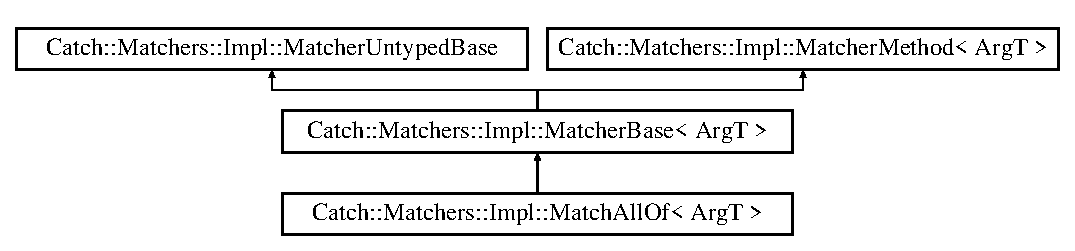
\includegraphics[height=2.926829cm]{struct_catch_1_1_matchers_1_1_impl_1_1_match_all_of}
\end{center}
\end{figure}
\subsection*{Public Member Functions}
\begin{DoxyCompactItemize}
\item 
bool \mbox{\hyperlink{struct_catch_1_1_matchers_1_1_impl_1_1_match_all_of_acfb377bda2c58ae62e6df9c3a8a89f8f}{match}} (ArgT const \&arg) const override
\item 
std\+::string \mbox{\hyperlink{struct_catch_1_1_matchers_1_1_impl_1_1_match_all_of_acbb9a083e93b546fd33c9235b644c40f}{describe}} () const override
\item 
\mbox{\hyperlink{struct_catch_1_1_matchers_1_1_impl_1_1_match_all_of}{Match\+All\+Of}}$<$ ArgT $>$ \& \mbox{\hyperlink{struct_catch_1_1_matchers_1_1_impl_1_1_match_all_of_a9d0e38b36474336498d627610db434f3}{operator\&\&}} (\mbox{\hyperlink{struct_catch_1_1_matchers_1_1_impl_1_1_matcher_base}{Matcher\+Base}}$<$ ArgT $>$ const \&other)
\end{DoxyCompactItemize}
\subsection*{Public Attributes}
\begin{DoxyCompactItemize}
\item 
std\+::vector$<$ \mbox{\hyperlink{struct_catch_1_1_matchers_1_1_impl_1_1_matcher_base}{Matcher\+Base}}$<$ ArgT $>$ const  $\ast$ $>$ \mbox{\hyperlink{struct_catch_1_1_matchers_1_1_impl_1_1_match_all_of_a98d6a2611f195a4a5c49f92fd877be9a}{m\+\_\+matchers}}
\end{DoxyCompactItemize}
\subsection*{Additional Inherited Members}


\subsection{Detailed Description}
\subsubsection*{template$<$typename ArgT$>$\newline
struct Catch\+::\+Matchers\+::\+Impl\+::\+Match\+All\+Of$<$ Arg\+T $>$}



Definition at line 2179 of file catch.\+hpp.



\subsection{Member Function Documentation}
\mbox{\Hypertarget{struct_catch_1_1_matchers_1_1_impl_1_1_match_all_of_acbb9a083e93b546fd33c9235b644c40f}\label{struct_catch_1_1_matchers_1_1_impl_1_1_match_all_of_acbb9a083e93b546fd33c9235b644c40f}} 
\index{Catch\+::\+Matchers\+::\+Impl\+::\+Match\+All\+Of@{Catch\+::\+Matchers\+::\+Impl\+::\+Match\+All\+Of}!describe@{describe}}
\index{describe@{describe}!Catch\+::\+Matchers\+::\+Impl\+::\+Match\+All\+Of@{Catch\+::\+Matchers\+::\+Impl\+::\+Match\+All\+Of}}
\subsubsection{\texorpdfstring{describe()}{describe()}}
{\footnotesize\ttfamily template$<$typename ArgT$>$ \\
std\+::string \mbox{\hyperlink{struct_catch_1_1_matchers_1_1_impl_1_1_match_all_of}{Catch\+::\+Matchers\+::\+Impl\+::\+Match\+All\+Of}}$<$ ArgT $>$\+::describe (\begin{DoxyParamCaption}{ }\end{DoxyParamCaption}) const\hspace{0.3cm}{\ttfamily [inline]}, {\ttfamily [override]}, {\ttfamily [virtual]}}



Implements \mbox{\hyperlink{class_catch_1_1_matchers_1_1_impl_1_1_matcher_untyped_base_a91d3a907dbfcbb596077df24f6e11fe2}{Catch\+::\+Matchers\+::\+Impl\+::\+Matcher\+Untyped\+Base}}.



Definition at line 2222 of file catch.\+hpp.

\mbox{\Hypertarget{struct_catch_1_1_matchers_1_1_impl_1_1_match_all_of_acfb377bda2c58ae62e6df9c3a8a89f8f}\label{struct_catch_1_1_matchers_1_1_impl_1_1_match_all_of_acfb377bda2c58ae62e6df9c3a8a89f8f}} 
\index{Catch\+::\+Matchers\+::\+Impl\+::\+Match\+All\+Of@{Catch\+::\+Matchers\+::\+Impl\+::\+Match\+All\+Of}!match@{match}}
\index{match@{match}!Catch\+::\+Matchers\+::\+Impl\+::\+Match\+All\+Of@{Catch\+::\+Matchers\+::\+Impl\+::\+Match\+All\+Of}}
\subsubsection{\texorpdfstring{match()}{match()}}
{\footnotesize\ttfamily template$<$typename ArgT$>$ \\
bool \mbox{\hyperlink{struct_catch_1_1_matchers_1_1_impl_1_1_match_all_of}{Catch\+::\+Matchers\+::\+Impl\+::\+Match\+All\+Of}}$<$ ArgT $>$\+::match (\begin{DoxyParamCaption}\item[{ArgT const \&}]{arg }\end{DoxyParamCaption}) const\hspace{0.3cm}{\ttfamily [inline]}, {\ttfamily [override]}, {\ttfamily [virtual]}}



Implements \mbox{\hyperlink{struct_catch_1_1_matchers_1_1_impl_1_1_matcher_method_ae0920ff9e817acf08e1bb0cbcb044e30}{Catch\+::\+Matchers\+::\+Impl\+::\+Matcher\+Method$<$ Arg\+T $>$}}.



Definition at line 2215 of file catch.\+hpp.

\mbox{\Hypertarget{struct_catch_1_1_matchers_1_1_impl_1_1_match_all_of_a9d0e38b36474336498d627610db434f3}\label{struct_catch_1_1_matchers_1_1_impl_1_1_match_all_of_a9d0e38b36474336498d627610db434f3}} 
\index{Catch\+::\+Matchers\+::\+Impl\+::\+Match\+All\+Of@{Catch\+::\+Matchers\+::\+Impl\+::\+Match\+All\+Of}!operator\&\&@{operator\&\&}}
\index{operator\&\&@{operator\&\&}!Catch\+::\+Matchers\+::\+Impl\+::\+Match\+All\+Of@{Catch\+::\+Matchers\+::\+Impl\+::\+Match\+All\+Of}}
\subsubsection{\texorpdfstring{operator\&\&()}{operator\&\&()}}
{\footnotesize\ttfamily template$<$typename ArgT$>$ \\
\mbox{\hyperlink{struct_catch_1_1_matchers_1_1_impl_1_1_match_all_of}{Match\+All\+Of}}$<$ArgT$>$\& \mbox{\hyperlink{struct_catch_1_1_matchers_1_1_impl_1_1_match_all_of}{Catch\+::\+Matchers\+::\+Impl\+::\+Match\+All\+Of}}$<$ ArgT $>$\+::operator \&\& (\begin{DoxyParamCaption}\item[{\mbox{\hyperlink{struct_catch_1_1_matchers_1_1_impl_1_1_matcher_base}{Matcher\+Base}}$<$ ArgT $>$ const \&}]{other }\end{DoxyParamCaption})\hspace{0.3cm}{\ttfamily [inline]}}



Definition at line 2238 of file catch.\+hpp.



\subsection{Member Data Documentation}
\mbox{\Hypertarget{struct_catch_1_1_matchers_1_1_impl_1_1_match_all_of_a98d6a2611f195a4a5c49f92fd877be9a}\label{struct_catch_1_1_matchers_1_1_impl_1_1_match_all_of_a98d6a2611f195a4a5c49f92fd877be9a}} 
\index{Catch\+::\+Matchers\+::\+Impl\+::\+Match\+All\+Of@{Catch\+::\+Matchers\+::\+Impl\+::\+Match\+All\+Of}!m\+\_\+matchers@{m\+\_\+matchers}}
\index{m\+\_\+matchers@{m\+\_\+matchers}!Catch\+::\+Matchers\+::\+Impl\+::\+Match\+All\+Of@{Catch\+::\+Matchers\+::\+Impl\+::\+Match\+All\+Of}}
\subsubsection{\texorpdfstring{m\+\_\+matchers}{m\_matchers}}
{\footnotesize\ttfamily template$<$typename ArgT$>$ \\
std\+::vector$<$\mbox{\hyperlink{struct_catch_1_1_matchers_1_1_impl_1_1_matcher_base}{Matcher\+Base}}$<$ArgT$>$ const$\ast$$>$ \mbox{\hyperlink{struct_catch_1_1_matchers_1_1_impl_1_1_match_all_of}{Catch\+::\+Matchers\+::\+Impl\+::\+Match\+All\+Of}}$<$ ArgT $>$\+::m\+\_\+matchers}



Definition at line 2243 of file catch.\+hpp.



The documentation for this struct was generated from the following file\+:\begin{DoxyCompactItemize}
\item 
D\+:/c++/block\+\_\+matrix-\/master/block\+\_\+matrix-\/master/test/\mbox{\hyperlink{catch_8hpp}{catch.\+hpp}}\end{DoxyCompactItemize}

\hypertarget{struct_catch_1_1_matchers_1_1_impl_1_1_match_any_of}{}\section{Catch\+:\+:Matchers\+:\+:Impl\+:\+:Match\+Any\+Of$<$ ArgT $>$ Struct Template Reference}
\label{struct_catch_1_1_matchers_1_1_impl_1_1_match_any_of}\index{Catch\+::\+Matchers\+::\+Impl\+::\+Match\+Any\+Of$<$ Arg\+T $>$@{Catch\+::\+Matchers\+::\+Impl\+::\+Match\+Any\+Of$<$ Arg\+T $>$}}


{\ttfamily \#include $<$catch.\+hpp$>$}

Inheritance diagram for Catch\+:\+:Matchers\+:\+:Impl\+:\+:Match\+Any\+Of$<$ ArgT $>$\+:\begin{figure}[H]
\begin{center}
\leavevmode
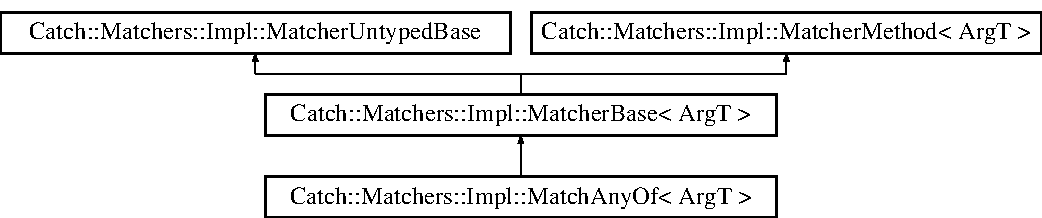
\includegraphics[height=2.926829cm]{struct_catch_1_1_matchers_1_1_impl_1_1_match_any_of}
\end{center}
\end{figure}
\subsection*{Public Member Functions}
\begin{DoxyCompactItemize}
\item 
bool \mbox{\hyperlink{struct_catch_1_1_matchers_1_1_impl_1_1_match_any_of_a8a3e8338f979e56277dcf553efb78dc0}{match}} (ArgT const \&arg) const override
\item 
std\+::string \mbox{\hyperlink{struct_catch_1_1_matchers_1_1_impl_1_1_match_any_of_a315285204df93d1f8e72f50dd66eb709}{describe}} () const override
\item 
\mbox{\hyperlink{struct_catch_1_1_matchers_1_1_impl_1_1_match_any_of}{Match\+Any\+Of}}$<$ ArgT $>$ \& \mbox{\hyperlink{struct_catch_1_1_matchers_1_1_impl_1_1_match_any_of_a44d7582dbe09fc31b9a5ba8a6367b506}{operator$\vert$$\vert$}} (\mbox{\hyperlink{struct_catch_1_1_matchers_1_1_impl_1_1_matcher_base}{Matcher\+Base}}$<$ ArgT $>$ const \&other)
\end{DoxyCompactItemize}
\subsection*{Public Attributes}
\begin{DoxyCompactItemize}
\item 
std\+::vector$<$ \mbox{\hyperlink{struct_catch_1_1_matchers_1_1_impl_1_1_matcher_base}{Matcher\+Base}}$<$ ArgT $>$ const  $\ast$ $>$ \mbox{\hyperlink{struct_catch_1_1_matchers_1_1_impl_1_1_match_any_of_a1fb1119e6110dc15b8d5262ec0aeddd5}{m\+\_\+matchers}}
\end{DoxyCompactItemize}
\subsection*{Additional Inherited Members}


\subsection{Detailed Description}
\subsubsection*{template$<$typename ArgT$>$\newline
struct Catch\+::\+Matchers\+::\+Impl\+::\+Match\+Any\+Of$<$ Arg\+T $>$}



Definition at line 2180 of file catch.\+hpp.



\subsection{Member Function Documentation}
\mbox{\Hypertarget{struct_catch_1_1_matchers_1_1_impl_1_1_match_any_of_a315285204df93d1f8e72f50dd66eb709}\label{struct_catch_1_1_matchers_1_1_impl_1_1_match_any_of_a315285204df93d1f8e72f50dd66eb709}} 
\index{Catch\+::\+Matchers\+::\+Impl\+::\+Match\+Any\+Of@{Catch\+::\+Matchers\+::\+Impl\+::\+Match\+Any\+Of}!describe@{describe}}
\index{describe@{describe}!Catch\+::\+Matchers\+::\+Impl\+::\+Match\+Any\+Of@{Catch\+::\+Matchers\+::\+Impl\+::\+Match\+Any\+Of}}
\subsubsection{\texorpdfstring{describe()}{describe()}}
{\footnotesize\ttfamily template$<$typename ArgT$>$ \\
std\+::string \mbox{\hyperlink{struct_catch_1_1_matchers_1_1_impl_1_1_match_any_of}{Catch\+::\+Matchers\+::\+Impl\+::\+Match\+Any\+Of}}$<$ ArgT $>$\+::describe (\begin{DoxyParamCaption}{ }\end{DoxyParamCaption}) const\hspace{0.3cm}{\ttfamily [inline]}, {\ttfamily [override]}, {\ttfamily [virtual]}}



Implements \mbox{\hyperlink{class_catch_1_1_matchers_1_1_impl_1_1_matcher_untyped_base_a91d3a907dbfcbb596077df24f6e11fe2}{Catch\+::\+Matchers\+::\+Impl\+::\+Matcher\+Untyped\+Base}}.



Definition at line 2255 of file catch.\+hpp.

\mbox{\Hypertarget{struct_catch_1_1_matchers_1_1_impl_1_1_match_any_of_a8a3e8338f979e56277dcf553efb78dc0}\label{struct_catch_1_1_matchers_1_1_impl_1_1_match_any_of_a8a3e8338f979e56277dcf553efb78dc0}} 
\index{Catch\+::\+Matchers\+::\+Impl\+::\+Match\+Any\+Of@{Catch\+::\+Matchers\+::\+Impl\+::\+Match\+Any\+Of}!match@{match}}
\index{match@{match}!Catch\+::\+Matchers\+::\+Impl\+::\+Match\+Any\+Of@{Catch\+::\+Matchers\+::\+Impl\+::\+Match\+Any\+Of}}
\subsubsection{\texorpdfstring{match()}{match()}}
{\footnotesize\ttfamily template$<$typename ArgT$>$ \\
bool \mbox{\hyperlink{struct_catch_1_1_matchers_1_1_impl_1_1_match_any_of}{Catch\+::\+Matchers\+::\+Impl\+::\+Match\+Any\+Of}}$<$ ArgT $>$\+::match (\begin{DoxyParamCaption}\item[{ArgT const \&}]{arg }\end{DoxyParamCaption}) const\hspace{0.3cm}{\ttfamily [inline]}, {\ttfamily [override]}, {\ttfamily [virtual]}}



Implements \mbox{\hyperlink{struct_catch_1_1_matchers_1_1_impl_1_1_matcher_method_ae0920ff9e817acf08e1bb0cbcb044e30}{Catch\+::\+Matchers\+::\+Impl\+::\+Matcher\+Method$<$ Arg\+T $>$}}.



Definition at line 2248 of file catch.\+hpp.

\mbox{\Hypertarget{struct_catch_1_1_matchers_1_1_impl_1_1_match_any_of_a44d7582dbe09fc31b9a5ba8a6367b506}\label{struct_catch_1_1_matchers_1_1_impl_1_1_match_any_of_a44d7582dbe09fc31b9a5ba8a6367b506}} 
\index{Catch\+::\+Matchers\+::\+Impl\+::\+Match\+Any\+Of@{Catch\+::\+Matchers\+::\+Impl\+::\+Match\+Any\+Of}!operator\texttt{"|}\texttt{"|}@{operator\texttt{"|}\texttt{"|}}}
\index{operator\texttt{"|}\texttt{"|}@{operator\texttt{"|}\texttt{"|}}!Catch\+::\+Matchers\+::\+Impl\+::\+Match\+Any\+Of@{Catch\+::\+Matchers\+::\+Impl\+::\+Match\+Any\+Of}}
\subsubsection{\texorpdfstring{operator\texttt{"|}\texttt{"|}()}{operator||()}}
{\footnotesize\ttfamily template$<$typename ArgT$>$ \\
\mbox{\hyperlink{struct_catch_1_1_matchers_1_1_impl_1_1_match_any_of}{Match\+Any\+Of}}$<$ArgT$>$\& \mbox{\hyperlink{struct_catch_1_1_matchers_1_1_impl_1_1_match_any_of}{Catch\+::\+Matchers\+::\+Impl\+::\+Match\+Any\+Of}}$<$ ArgT $>$\+::operator$\vert$$\vert$ (\begin{DoxyParamCaption}\item[{\mbox{\hyperlink{struct_catch_1_1_matchers_1_1_impl_1_1_matcher_base}{Matcher\+Base}}$<$ ArgT $>$ const \&}]{other }\end{DoxyParamCaption})\hspace{0.3cm}{\ttfamily [inline]}}



Definition at line 2271 of file catch.\+hpp.



\subsection{Member Data Documentation}
\mbox{\Hypertarget{struct_catch_1_1_matchers_1_1_impl_1_1_match_any_of_a1fb1119e6110dc15b8d5262ec0aeddd5}\label{struct_catch_1_1_matchers_1_1_impl_1_1_match_any_of_a1fb1119e6110dc15b8d5262ec0aeddd5}} 
\index{Catch\+::\+Matchers\+::\+Impl\+::\+Match\+Any\+Of@{Catch\+::\+Matchers\+::\+Impl\+::\+Match\+Any\+Of}!m\+\_\+matchers@{m\+\_\+matchers}}
\index{m\+\_\+matchers@{m\+\_\+matchers}!Catch\+::\+Matchers\+::\+Impl\+::\+Match\+Any\+Of@{Catch\+::\+Matchers\+::\+Impl\+::\+Match\+Any\+Of}}
\subsubsection{\texorpdfstring{m\+\_\+matchers}{m\_matchers}}
{\footnotesize\ttfamily template$<$typename ArgT$>$ \\
std\+::vector$<$\mbox{\hyperlink{struct_catch_1_1_matchers_1_1_impl_1_1_matcher_base}{Matcher\+Base}}$<$ArgT$>$ const$\ast$$>$ \mbox{\hyperlink{struct_catch_1_1_matchers_1_1_impl_1_1_match_any_of}{Catch\+::\+Matchers\+::\+Impl\+::\+Match\+Any\+Of}}$<$ ArgT $>$\+::m\+\_\+matchers}



Definition at line 2276 of file catch.\+hpp.



The documentation for this struct was generated from the following file\+:\begin{DoxyCompactItemize}
\item 
D\+:/c++/block\+\_\+matrix-\/master/block\+\_\+matrix-\/master/test/\mbox{\hyperlink{catch_8hpp}{catch.\+hpp}}\end{DoxyCompactItemize}

\hypertarget{struct_catch_1_1_matchers_1_1_impl_1_1_matcher_base}{}\section{Catch\+:\+:Matchers\+:\+:Impl\+:\+:Matcher\+Base$<$ T $>$ Struct Template Reference}
\label{struct_catch_1_1_matchers_1_1_impl_1_1_matcher_base}\index{Catch\+::\+Matchers\+::\+Impl\+::\+Matcher\+Base$<$ T $>$@{Catch\+::\+Matchers\+::\+Impl\+::\+Matcher\+Base$<$ T $>$}}


{\ttfamily \#include $<$catch.\+hpp$>$}

Inheritance diagram for Catch\+:\+:Matchers\+:\+:Impl\+:\+:Matcher\+Base$<$ T $>$\+:\begin{figure}[H]
\begin{center}
\leavevmode
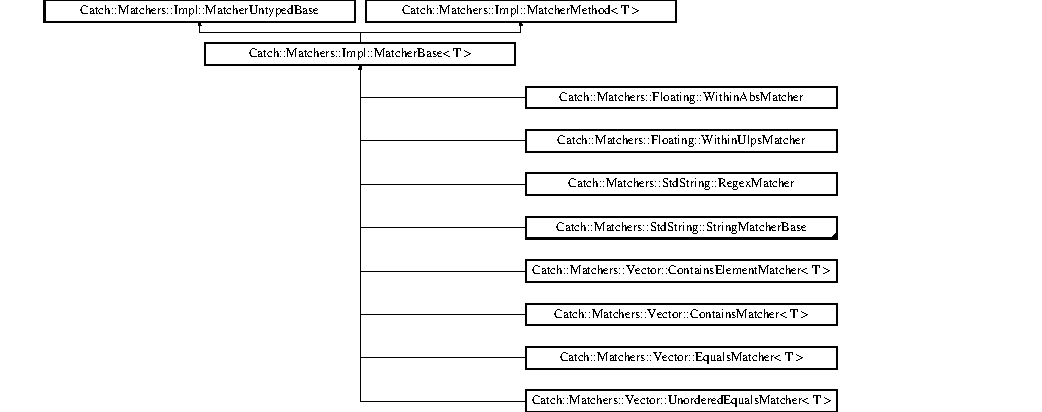
\includegraphics[height=5.539070cm]{struct_catch_1_1_matchers_1_1_impl_1_1_matcher_base}
\end{center}
\end{figure}
\subsection*{Public Member Functions}
\begin{DoxyCompactItemize}
\item 
\mbox{\hyperlink{struct_catch_1_1_matchers_1_1_impl_1_1_match_all_of}{Match\+All\+Of}}$<$ T $>$ \mbox{\hyperlink{struct_catch_1_1_matchers_1_1_impl_1_1_matcher_base_a23c336f6d9457735ddc8dc7ea864d7c9}{operator\&\&}} (\mbox{\hyperlink{struct_catch_1_1_matchers_1_1_impl_1_1_matcher_base}{Matcher\+Base}} const \&other) const
\item 
\mbox{\hyperlink{struct_catch_1_1_matchers_1_1_impl_1_1_match_any_of}{Match\+Any\+Of}}$<$ T $>$ \mbox{\hyperlink{struct_catch_1_1_matchers_1_1_impl_1_1_matcher_base_a5f8542b8f1567a6f9c65d0a6da7b679b}{operator$\vert$$\vert$}} (\mbox{\hyperlink{struct_catch_1_1_matchers_1_1_impl_1_1_matcher_base}{Matcher\+Base}} const \&other) const
\item 
\mbox{\hyperlink{struct_catch_1_1_matchers_1_1_impl_1_1_match_not_of}{Match\+Not\+Of}}$<$ T $>$ \mbox{\hyperlink{struct_catch_1_1_matchers_1_1_impl_1_1_matcher_base_a5bb94bf2ff5c7ef73b7c11eb173bdf3b}{operator!}} () const
\end{DoxyCompactItemize}
\subsection*{Additional Inherited Members}


\subsection{Detailed Description}
\subsubsection*{template$<$typename T$>$\newline
struct Catch\+::\+Matchers\+::\+Impl\+::\+Matcher\+Base$<$ T $>$}



Definition at line 2206 of file catch.\+hpp.



\subsection{Member Function Documentation}
\mbox{\Hypertarget{struct_catch_1_1_matchers_1_1_impl_1_1_matcher_base_a5bb94bf2ff5c7ef73b7c11eb173bdf3b}\label{struct_catch_1_1_matchers_1_1_impl_1_1_matcher_base_a5bb94bf2ff5c7ef73b7c11eb173bdf3b}} 
\index{Catch\+::\+Matchers\+::\+Impl\+::\+Matcher\+Base@{Catch\+::\+Matchers\+::\+Impl\+::\+Matcher\+Base}!operator"!@{operator"!}}
\index{operator"!@{operator"!}!Catch\+::\+Matchers\+::\+Impl\+::\+Matcher\+Base@{Catch\+::\+Matchers\+::\+Impl\+::\+Matcher\+Base}}
\subsubsection{\texorpdfstring{operator"!()}{operator!()}}
{\footnotesize\ttfamily template$<$typename T $>$ \\
\mbox{\hyperlink{struct_catch_1_1_matchers_1_1_impl_1_1_match_not_of}{Match\+Not\+Of}}$<$ T $>$ \mbox{\hyperlink{struct_catch_1_1_matchers_1_1_impl_1_1_matcher_base}{Catch\+::\+Matchers\+::\+Impl\+::\+Matcher\+Base}}$<$ T $>$\+::operator! (\begin{DoxyParamCaption}{ }\end{DoxyParamCaption}) const}



Definition at line 2303 of file catch.\+hpp.

\mbox{\Hypertarget{struct_catch_1_1_matchers_1_1_impl_1_1_matcher_base_a23c336f6d9457735ddc8dc7ea864d7c9}\label{struct_catch_1_1_matchers_1_1_impl_1_1_matcher_base_a23c336f6d9457735ddc8dc7ea864d7c9}} 
\index{Catch\+::\+Matchers\+::\+Impl\+::\+Matcher\+Base@{Catch\+::\+Matchers\+::\+Impl\+::\+Matcher\+Base}!operator\&\&@{operator\&\&}}
\index{operator\&\&@{operator\&\&}!Catch\+::\+Matchers\+::\+Impl\+::\+Matcher\+Base@{Catch\+::\+Matchers\+::\+Impl\+::\+Matcher\+Base}}
\subsubsection{\texorpdfstring{operator\&\&()}{operator\&\&()}}
{\footnotesize\ttfamily template$<$typename T$>$ \\
\mbox{\hyperlink{struct_catch_1_1_matchers_1_1_impl_1_1_match_all_of}{Match\+All\+Of}}$<$T$>$ \mbox{\hyperlink{struct_catch_1_1_matchers_1_1_impl_1_1_matcher_base}{Catch\+::\+Matchers\+::\+Impl\+::\+Matcher\+Base}}$<$ T $>$\+::operator \&\& (\begin{DoxyParamCaption}\item[{\mbox{\hyperlink{struct_catch_1_1_matchers_1_1_impl_1_1_matcher_base}{Matcher\+Base}}$<$ T $>$ const \&}]{other }\end{DoxyParamCaption}) const}

\mbox{\Hypertarget{struct_catch_1_1_matchers_1_1_impl_1_1_matcher_base_a5f8542b8f1567a6f9c65d0a6da7b679b}\label{struct_catch_1_1_matchers_1_1_impl_1_1_matcher_base_a5f8542b8f1567a6f9c65d0a6da7b679b}} 
\index{Catch\+::\+Matchers\+::\+Impl\+::\+Matcher\+Base@{Catch\+::\+Matchers\+::\+Impl\+::\+Matcher\+Base}!operator\texttt{"|}\texttt{"|}@{operator\texttt{"|}\texttt{"|}}}
\index{operator\texttt{"|}\texttt{"|}@{operator\texttt{"|}\texttt{"|}}!Catch\+::\+Matchers\+::\+Impl\+::\+Matcher\+Base@{Catch\+::\+Matchers\+::\+Impl\+::\+Matcher\+Base}}
\subsubsection{\texorpdfstring{operator\texttt{"|}\texttt{"|}()}{operator||()}}
{\footnotesize\ttfamily template$<$typename T $>$ \\
\mbox{\hyperlink{struct_catch_1_1_matchers_1_1_impl_1_1_match_any_of}{Match\+Any\+Of}}$<$ T $>$ \mbox{\hyperlink{struct_catch_1_1_matchers_1_1_impl_1_1_matcher_base}{Catch\+::\+Matchers\+::\+Impl\+::\+Matcher\+Base}}$<$ T $>$\+::operator$\vert$$\vert$ (\begin{DoxyParamCaption}\item[{\mbox{\hyperlink{struct_catch_1_1_matchers_1_1_impl_1_1_matcher_base}{Matcher\+Base}}$<$ T $>$ const \&}]{other }\end{DoxyParamCaption}) const}



Definition at line 2299 of file catch.\+hpp.



The documentation for this struct was generated from the following file\+:\begin{DoxyCompactItemize}
\item 
D\+:/c++/block\+\_\+matrix-\/master/block\+\_\+matrix-\/master/test/\mbox{\hyperlink{catch_8hpp}{catch.\+hpp}}\end{DoxyCompactItemize}

\hypertarget{struct_catch_1_1_matchers_1_1_impl_1_1_matcher_method}{}\section{Catch\+:\+:Matchers\+:\+:Impl\+:\+:Matcher\+Method$<$ ObjectT $>$ Struct Template Reference}
\label{struct_catch_1_1_matchers_1_1_impl_1_1_matcher_method}\index{Catch\+::\+Matchers\+::\+Impl\+::\+Matcher\+Method$<$ Object\+T $>$@{Catch\+::\+Matchers\+::\+Impl\+::\+Matcher\+Method$<$ Object\+T $>$}}


{\ttfamily \#include $<$catch.\+hpp$>$}

\subsection*{Public Member Functions}
\begin{DoxyCompactItemize}
\item 
virtual bool \mbox{\hyperlink{struct_catch_1_1_matchers_1_1_impl_1_1_matcher_method_ae0920ff9e817acf08e1bb0cbcb044e30}{match}} (ObjectT const \&arg) const =0
\end{DoxyCompactItemize}


\subsection{Detailed Description}
\subsubsection*{template$<$typename ObjectT$>$\newline
struct Catch\+::\+Matchers\+::\+Impl\+::\+Matcher\+Method$<$ Object\+T $>$}



Definition at line 2197 of file catch.\+hpp.



\subsection{Member Function Documentation}
\mbox{\Hypertarget{struct_catch_1_1_matchers_1_1_impl_1_1_matcher_method_ae0920ff9e817acf08e1bb0cbcb044e30}\label{struct_catch_1_1_matchers_1_1_impl_1_1_matcher_method_ae0920ff9e817acf08e1bb0cbcb044e30}} 
\index{Catch\+::\+Matchers\+::\+Impl\+::\+Matcher\+Method@{Catch\+::\+Matchers\+::\+Impl\+::\+Matcher\+Method}!match@{match}}
\index{match@{match}!Catch\+::\+Matchers\+::\+Impl\+::\+Matcher\+Method@{Catch\+::\+Matchers\+::\+Impl\+::\+Matcher\+Method}}
\subsubsection{\texorpdfstring{match()}{match()}}
{\footnotesize\ttfamily template$<$typename ObjectT$>$ \\
virtual bool \mbox{\hyperlink{struct_catch_1_1_matchers_1_1_impl_1_1_matcher_method}{Catch\+::\+Matchers\+::\+Impl\+::\+Matcher\+Method}}$<$ ObjectT $>$\+::match (\begin{DoxyParamCaption}\item[{ObjectT const \&}]{arg }\end{DoxyParamCaption}) const\hspace{0.3cm}{\ttfamily [pure virtual]}}



Implemented in \mbox{\hyperlink{struct_catch_1_1_matchers_1_1_impl_1_1_match_not_of_a181d693c0258e582d80dc6117a1f2b66}{Catch\+::\+Matchers\+::\+Impl\+::\+Match\+Not\+Of$<$ Arg\+T $>$}}, \mbox{\hyperlink{struct_catch_1_1_matchers_1_1_impl_1_1_match_any_of_a8a3e8338f979e56277dcf553efb78dc0}{Catch\+::\+Matchers\+::\+Impl\+::\+Match\+Any\+Of$<$ Arg\+T $>$}}, and \mbox{\hyperlink{struct_catch_1_1_matchers_1_1_impl_1_1_match_all_of_acfb377bda2c58ae62e6df9c3a8a89f8f}{Catch\+::\+Matchers\+::\+Impl\+::\+Match\+All\+Of$<$ Arg\+T $>$}}.



The documentation for this struct was generated from the following file\+:\begin{DoxyCompactItemize}
\item 
D\+:/c++/block\+\_\+matrix-\/master/block\+\_\+matrix-\/master/test/\mbox{\hyperlink{catch_8hpp}{catch.\+hpp}}\end{DoxyCompactItemize}

\hypertarget{struct_catch_1_1_matchers_1_1_impl_1_1_matcher_method_3_01_ptr_t_01_5_01_4}{}\section{Catch\+:\+:Matchers\+:\+:Impl\+:\+:Matcher\+Method$<$ PtrT $\ast$ $>$ Struct Template Reference}
\label{struct_catch_1_1_matchers_1_1_impl_1_1_matcher_method_3_01_ptr_t_01_5_01_4}\index{Catch\+::\+Matchers\+::\+Impl\+::\+Matcher\+Method$<$ Ptr\+T $\ast$ $>$@{Catch\+::\+Matchers\+::\+Impl\+::\+Matcher\+Method$<$ Ptr\+T $\ast$ $>$}}


{\ttfamily \#include $<$catch.\+hpp$>$}

\subsection*{Public Member Functions}
\begin{DoxyCompactItemize}
\item 
virtual bool \mbox{\hyperlink{struct_catch_1_1_matchers_1_1_impl_1_1_matcher_method_3_01_ptr_t_01_5_01_4_a5fdd64f9509724f32ffc73cb320181d1}{match}} (PtrT $\ast$arg) const =0
\end{DoxyCompactItemize}


\subsection{Detailed Description}
\subsubsection*{template$<$typename PtrT$>$\newline
struct Catch\+::\+Matchers\+::\+Impl\+::\+Matcher\+Method$<$ Ptr\+T $\ast$ $>$}



Definition at line 2201 of file catch.\+hpp.



\subsection{Member Function Documentation}
\mbox{\Hypertarget{struct_catch_1_1_matchers_1_1_impl_1_1_matcher_method_3_01_ptr_t_01_5_01_4_a5fdd64f9509724f32ffc73cb320181d1}\label{struct_catch_1_1_matchers_1_1_impl_1_1_matcher_method_3_01_ptr_t_01_5_01_4_a5fdd64f9509724f32ffc73cb320181d1}} 
\index{Catch\+::\+Matchers\+::\+Impl\+::\+Matcher\+Method$<$ Ptr\+T $\ast$ $>$@{Catch\+::\+Matchers\+::\+Impl\+::\+Matcher\+Method$<$ Ptr\+T $\ast$ $>$}!match@{match}}
\index{match@{match}!Catch\+::\+Matchers\+::\+Impl\+::\+Matcher\+Method$<$ Ptr\+T $\ast$ $>$@{Catch\+::\+Matchers\+::\+Impl\+::\+Matcher\+Method$<$ Ptr\+T $\ast$ $>$}}
\subsubsection{\texorpdfstring{match()}{match()}}
{\footnotesize\ttfamily template$<$typename PtrT $>$ \\
virtual bool \mbox{\hyperlink{struct_catch_1_1_matchers_1_1_impl_1_1_matcher_method}{Catch\+::\+Matchers\+::\+Impl\+::\+Matcher\+Method}}$<$ PtrT $\ast$ $>$\+::match (\begin{DoxyParamCaption}\item[{PtrT $\ast$}]{arg }\end{DoxyParamCaption}) const\hspace{0.3cm}{\ttfamily [pure virtual]}}



The documentation for this struct was generated from the following file\+:\begin{DoxyCompactItemize}
\item 
D\+:/c++/block\+\_\+matrix-\/master/block\+\_\+matrix-\/master/test/\mbox{\hyperlink{catch_8hpp}{catch.\+hpp}}\end{DoxyCompactItemize}

\hypertarget{class_catch_1_1_matchers_1_1_impl_1_1_matcher_untyped_base}{}\section{Catch\+:\+:Matchers\+:\+:Impl\+:\+:Matcher\+Untyped\+Base Class Reference}
\label{class_catch_1_1_matchers_1_1_impl_1_1_matcher_untyped_base}\index{Catch\+::\+Matchers\+::\+Impl\+::\+Matcher\+Untyped\+Base@{Catch\+::\+Matchers\+::\+Impl\+::\+Matcher\+Untyped\+Base}}


{\ttfamily \#include $<$catch.\+hpp$>$}

Inheritance diagram for Catch\+:\+:Matchers\+:\+:Impl\+:\+:Matcher\+Untyped\+Base\+:\begin{figure}[H]
\begin{center}
\leavevmode
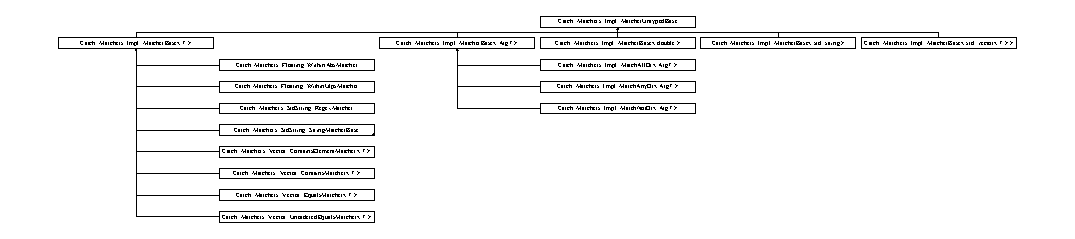
\includegraphics[height=2.769535cm]{class_catch_1_1_matchers_1_1_impl_1_1_matcher_untyped_base}
\end{center}
\end{figure}
\subsection*{Public Member Functions}
\begin{DoxyCompactItemize}
\item 
\mbox{\hyperlink{class_catch_1_1_matchers_1_1_impl_1_1_matcher_untyped_base_ab65764dc245d85e2b268d3be870b650a}{Matcher\+Untyped\+Base}} ()=default
\item 
\mbox{\hyperlink{class_catch_1_1_matchers_1_1_impl_1_1_matcher_untyped_base_a985fd3c3ffcc9f2e8dc7a330130040b0}{Matcher\+Untyped\+Base}} (\mbox{\hyperlink{class_catch_1_1_matchers_1_1_impl_1_1_matcher_untyped_base}{Matcher\+Untyped\+Base}} const \&)=default
\item 
\mbox{\hyperlink{class_catch_1_1_matchers_1_1_impl_1_1_matcher_untyped_base}{Matcher\+Untyped\+Base}} \& \mbox{\hyperlink{class_catch_1_1_matchers_1_1_impl_1_1_matcher_untyped_base_a62668ccc47b64a9094dcb6413f9af80b}{operator=}} (\mbox{\hyperlink{class_catch_1_1_matchers_1_1_impl_1_1_matcher_untyped_base}{Matcher\+Untyped\+Base}} const \&)=delete
\item 
std\+::string \mbox{\hyperlink{class_catch_1_1_matchers_1_1_impl_1_1_matcher_untyped_base_a5982c7c80ca71dfe2298babadad7a453}{to\+String}} () const
\end{DoxyCompactItemize}
\subsection*{Protected Member Functions}
\begin{DoxyCompactItemize}
\item 
virtual \mbox{\hyperlink{class_catch_1_1_matchers_1_1_impl_1_1_matcher_untyped_base_a853be93ce33f71b5abede38081c79e9d}{$\sim$\+Matcher\+Untyped\+Base}} ()
\item 
virtual std\+::string \mbox{\hyperlink{class_catch_1_1_matchers_1_1_impl_1_1_matcher_untyped_base_a91d3a907dbfcbb596077df24f6e11fe2}{describe}} () const =0
\end{DoxyCompactItemize}
\subsection*{Protected Attributes}
\begin{DoxyCompactItemize}
\item 
std\+::string \mbox{\hyperlink{class_catch_1_1_matchers_1_1_impl_1_1_matcher_untyped_base_a951095c462657e7097a9a6dc4dde813f}{m\+\_\+cached\+To\+String}}
\end{DoxyCompactItemize}


\subsection{Detailed Description}


Definition at line 2183 of file catch.\+hpp.



\subsection{Constructor \& Destructor Documentation}
\mbox{\Hypertarget{class_catch_1_1_matchers_1_1_impl_1_1_matcher_untyped_base_ab65764dc245d85e2b268d3be870b650a}\label{class_catch_1_1_matchers_1_1_impl_1_1_matcher_untyped_base_ab65764dc245d85e2b268d3be870b650a}} 
\index{Catch\+::\+Matchers\+::\+Impl\+::\+Matcher\+Untyped\+Base@{Catch\+::\+Matchers\+::\+Impl\+::\+Matcher\+Untyped\+Base}!Matcher\+Untyped\+Base@{Matcher\+Untyped\+Base}}
\index{Matcher\+Untyped\+Base@{Matcher\+Untyped\+Base}!Catch\+::\+Matchers\+::\+Impl\+::\+Matcher\+Untyped\+Base@{Catch\+::\+Matchers\+::\+Impl\+::\+Matcher\+Untyped\+Base}}
\subsubsection{\texorpdfstring{Matcher\+Untyped\+Base()}{MatcherUntypedBase()}\hspace{0.1cm}{\footnotesize\ttfamily [1/2]}}
{\footnotesize\ttfamily Catch\+::\+Matchers\+::\+Impl\+::\+Matcher\+Untyped\+Base\+::\+Matcher\+Untyped\+Base (\begin{DoxyParamCaption}{ }\end{DoxyParamCaption})\hspace{0.3cm}{\ttfamily [default]}}

\mbox{\Hypertarget{class_catch_1_1_matchers_1_1_impl_1_1_matcher_untyped_base_a985fd3c3ffcc9f2e8dc7a330130040b0}\label{class_catch_1_1_matchers_1_1_impl_1_1_matcher_untyped_base_a985fd3c3ffcc9f2e8dc7a330130040b0}} 
\index{Catch\+::\+Matchers\+::\+Impl\+::\+Matcher\+Untyped\+Base@{Catch\+::\+Matchers\+::\+Impl\+::\+Matcher\+Untyped\+Base}!Matcher\+Untyped\+Base@{Matcher\+Untyped\+Base}}
\index{Matcher\+Untyped\+Base@{Matcher\+Untyped\+Base}!Catch\+::\+Matchers\+::\+Impl\+::\+Matcher\+Untyped\+Base@{Catch\+::\+Matchers\+::\+Impl\+::\+Matcher\+Untyped\+Base}}
\subsubsection{\texorpdfstring{Matcher\+Untyped\+Base()}{MatcherUntypedBase()}\hspace{0.1cm}{\footnotesize\ttfamily [2/2]}}
{\footnotesize\ttfamily Catch\+::\+Matchers\+::\+Impl\+::\+Matcher\+Untyped\+Base\+::\+Matcher\+Untyped\+Base (\begin{DoxyParamCaption}\item[{\mbox{\hyperlink{class_catch_1_1_matchers_1_1_impl_1_1_matcher_untyped_base}{Matcher\+Untyped\+Base}} const \&}]{ }\end{DoxyParamCaption})\hspace{0.3cm}{\ttfamily [default]}}

\mbox{\Hypertarget{class_catch_1_1_matchers_1_1_impl_1_1_matcher_untyped_base_a853be93ce33f71b5abede38081c79e9d}\label{class_catch_1_1_matchers_1_1_impl_1_1_matcher_untyped_base_a853be93ce33f71b5abede38081c79e9d}} 
\index{Catch\+::\+Matchers\+::\+Impl\+::\+Matcher\+Untyped\+Base@{Catch\+::\+Matchers\+::\+Impl\+::\+Matcher\+Untyped\+Base}!````~Matcher\+Untyped\+Base@{$\sim$\+Matcher\+Untyped\+Base}}
\index{````~Matcher\+Untyped\+Base@{$\sim$\+Matcher\+Untyped\+Base}!Catch\+::\+Matchers\+::\+Impl\+::\+Matcher\+Untyped\+Base@{Catch\+::\+Matchers\+::\+Impl\+::\+Matcher\+Untyped\+Base}}
\subsubsection{\texorpdfstring{$\sim$\+Matcher\+Untyped\+Base()}{~MatcherUntypedBase()}}
{\footnotesize\ttfamily virtual Catch\+::\+Matchers\+::\+Impl\+::\+Matcher\+Untyped\+Base\+::$\sim$\+Matcher\+Untyped\+Base (\begin{DoxyParamCaption}{ }\end{DoxyParamCaption})\hspace{0.3cm}{\ttfamily [protected]}, {\ttfamily [virtual]}}



\subsection{Member Function Documentation}
\mbox{\Hypertarget{class_catch_1_1_matchers_1_1_impl_1_1_matcher_untyped_base_a91d3a907dbfcbb596077df24f6e11fe2}\label{class_catch_1_1_matchers_1_1_impl_1_1_matcher_untyped_base_a91d3a907dbfcbb596077df24f6e11fe2}} 
\index{Catch\+::\+Matchers\+::\+Impl\+::\+Matcher\+Untyped\+Base@{Catch\+::\+Matchers\+::\+Impl\+::\+Matcher\+Untyped\+Base}!describe@{describe}}
\index{describe@{describe}!Catch\+::\+Matchers\+::\+Impl\+::\+Matcher\+Untyped\+Base@{Catch\+::\+Matchers\+::\+Impl\+::\+Matcher\+Untyped\+Base}}
\subsubsection{\texorpdfstring{describe()}{describe()}}
{\footnotesize\ttfamily virtual std\+::string Catch\+::\+Matchers\+::\+Impl\+::\+Matcher\+Untyped\+Base\+::describe (\begin{DoxyParamCaption}{ }\end{DoxyParamCaption}) const\hspace{0.3cm}{\ttfamily [protected]}, {\ttfamily [pure virtual]}}



Implemented in \mbox{\hyperlink{struct_catch_1_1_matchers_1_1_vector_1_1_unordered_equals_matcher_a7202d811200317abc58c844f663823df}{Catch\+::\+Matchers\+::\+Vector\+::\+Unordered\+Equals\+Matcher$<$ T $>$}}, \mbox{\hyperlink{struct_catch_1_1_matchers_1_1_vector_1_1_equals_matcher_a36b5f7ecada4081d6c65bebe8ddea6f4}{Catch\+::\+Matchers\+::\+Vector\+::\+Equals\+Matcher$<$ T $>$}}, \mbox{\hyperlink{struct_catch_1_1_matchers_1_1_vector_1_1_contains_matcher_abe6a9ea3d6506c9a1f75ff524f35832e}{Catch\+::\+Matchers\+::\+Vector\+::\+Contains\+Matcher$<$ T $>$}}, \mbox{\hyperlink{struct_catch_1_1_matchers_1_1_vector_1_1_contains_element_matcher_aea3b674389a0afd82af6ba4b10f86ae6}{Catch\+::\+Matchers\+::\+Vector\+::\+Contains\+Element\+Matcher$<$ T $>$}}, \mbox{\hyperlink{struct_catch_1_1_matchers_1_1_std_string_1_1_regex_matcher_a1f788cd5258c987e5043f6c7f43adeb9}{Catch\+::\+Matchers\+::\+Std\+String\+::\+Regex\+Matcher}}, \mbox{\hyperlink{struct_catch_1_1_matchers_1_1_std_string_1_1_string_matcher_base_a47af030f8cea42a601ffb1000eea5cca}{Catch\+::\+Matchers\+::\+Std\+String\+::\+String\+Matcher\+Base}}, \mbox{\hyperlink{struct_catch_1_1_matchers_1_1_floating_1_1_within_ulps_matcher_ad9bc8bb7f3abd326580a4bf6cf369b1b}{Catch\+::\+Matchers\+::\+Floating\+::\+Within\+Ulps\+Matcher}}, \mbox{\hyperlink{struct_catch_1_1_matchers_1_1_floating_1_1_within_abs_matcher_a206a738680f8767af31d3f1835afff3f}{Catch\+::\+Matchers\+::\+Floating\+::\+Within\+Abs\+Matcher}}, \mbox{\hyperlink{struct_catch_1_1_matchers_1_1_impl_1_1_match_not_of_ac5fb4ef6a9069d23a4098c3c818f06b0}{Catch\+::\+Matchers\+::\+Impl\+::\+Match\+Not\+Of$<$ Arg\+T $>$}}, \mbox{\hyperlink{struct_catch_1_1_matchers_1_1_impl_1_1_match_any_of_a315285204df93d1f8e72f50dd66eb709}{Catch\+::\+Matchers\+::\+Impl\+::\+Match\+Any\+Of$<$ Arg\+T $>$}}, and \mbox{\hyperlink{struct_catch_1_1_matchers_1_1_impl_1_1_match_all_of_acbb9a083e93b546fd33c9235b644c40f}{Catch\+::\+Matchers\+::\+Impl\+::\+Match\+All\+Of$<$ Arg\+T $>$}}.

\mbox{\Hypertarget{class_catch_1_1_matchers_1_1_impl_1_1_matcher_untyped_base_a62668ccc47b64a9094dcb6413f9af80b}\label{class_catch_1_1_matchers_1_1_impl_1_1_matcher_untyped_base_a62668ccc47b64a9094dcb6413f9af80b}} 
\index{Catch\+::\+Matchers\+::\+Impl\+::\+Matcher\+Untyped\+Base@{Catch\+::\+Matchers\+::\+Impl\+::\+Matcher\+Untyped\+Base}!operator=@{operator=}}
\index{operator=@{operator=}!Catch\+::\+Matchers\+::\+Impl\+::\+Matcher\+Untyped\+Base@{Catch\+::\+Matchers\+::\+Impl\+::\+Matcher\+Untyped\+Base}}
\subsubsection{\texorpdfstring{operator=()}{operator=()}}
{\footnotesize\ttfamily \mbox{\hyperlink{class_catch_1_1_matchers_1_1_impl_1_1_matcher_untyped_base}{Matcher\+Untyped\+Base}}\& Catch\+::\+Matchers\+::\+Impl\+::\+Matcher\+Untyped\+Base\+::operator= (\begin{DoxyParamCaption}\item[{\mbox{\hyperlink{class_catch_1_1_matchers_1_1_impl_1_1_matcher_untyped_base}{Matcher\+Untyped\+Base}} const \&}]{ }\end{DoxyParamCaption})\hspace{0.3cm}{\ttfamily [delete]}}

\mbox{\Hypertarget{class_catch_1_1_matchers_1_1_impl_1_1_matcher_untyped_base_a5982c7c80ca71dfe2298babadad7a453}\label{class_catch_1_1_matchers_1_1_impl_1_1_matcher_untyped_base_a5982c7c80ca71dfe2298babadad7a453}} 
\index{Catch\+::\+Matchers\+::\+Impl\+::\+Matcher\+Untyped\+Base@{Catch\+::\+Matchers\+::\+Impl\+::\+Matcher\+Untyped\+Base}!to\+String@{to\+String}}
\index{to\+String@{to\+String}!Catch\+::\+Matchers\+::\+Impl\+::\+Matcher\+Untyped\+Base@{Catch\+::\+Matchers\+::\+Impl\+::\+Matcher\+Untyped\+Base}}
\subsubsection{\texorpdfstring{to\+String()}{toString()}}
{\footnotesize\ttfamily std\+::string Catch\+::\+Matchers\+::\+Impl\+::\+Matcher\+Untyped\+Base\+::to\+String (\begin{DoxyParamCaption}{ }\end{DoxyParamCaption}) const}



\subsection{Member Data Documentation}
\mbox{\Hypertarget{class_catch_1_1_matchers_1_1_impl_1_1_matcher_untyped_base_a951095c462657e7097a9a6dc4dde813f}\label{class_catch_1_1_matchers_1_1_impl_1_1_matcher_untyped_base_a951095c462657e7097a9a6dc4dde813f}} 
\index{Catch\+::\+Matchers\+::\+Impl\+::\+Matcher\+Untyped\+Base@{Catch\+::\+Matchers\+::\+Impl\+::\+Matcher\+Untyped\+Base}!m\+\_\+cached\+To\+String@{m\+\_\+cached\+To\+String}}
\index{m\+\_\+cached\+To\+String@{m\+\_\+cached\+To\+String}!Catch\+::\+Matchers\+::\+Impl\+::\+Matcher\+Untyped\+Base@{Catch\+::\+Matchers\+::\+Impl\+::\+Matcher\+Untyped\+Base}}
\subsubsection{\texorpdfstring{m\+\_\+cached\+To\+String}{m\_cachedToString}}
{\footnotesize\ttfamily std\+::string Catch\+::\+Matchers\+::\+Impl\+::\+Matcher\+Untyped\+Base\+::m\+\_\+cached\+To\+String\hspace{0.3cm}{\ttfamily [mutable]}, {\ttfamily [protected]}}



Definition at line 2193 of file catch.\+hpp.



The documentation for this class was generated from the following file\+:\begin{DoxyCompactItemize}
\item 
D\+:/c++/block\+\_\+matrix-\/master/block\+\_\+matrix-\/master/test/\mbox{\hyperlink{catch_8hpp}{catch.\+hpp}}\end{DoxyCompactItemize}

\hypertarget{class_catch_1_1_match_expr}{}\section{Catch\+:\+:Match\+Expr$<$ ArgT, MatcherT $>$ Class Template Reference}
\label{class_catch_1_1_match_expr}\index{Catch\+::\+Match\+Expr$<$ Arg\+T, Matcher\+T $>$@{Catch\+::\+Match\+Expr$<$ Arg\+T, Matcher\+T $>$}}


{\ttfamily \#include $<$catch.\+hpp$>$}

Inheritance diagram for Catch\+:\+:Match\+Expr$<$ ArgT, MatcherT $>$\+:\begin{figure}[H]
\begin{center}
\leavevmode
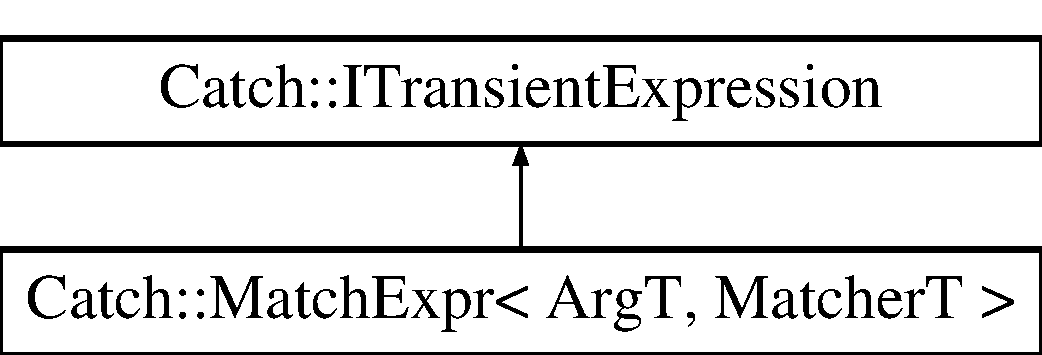
\includegraphics[height=2.000000cm]{class_catch_1_1_match_expr}
\end{center}
\end{figure}
\subsection*{Public Member Functions}
\begin{DoxyCompactItemize}
\item 
\mbox{\hyperlink{class_catch_1_1_match_expr_ab5b9ecc4fb9e91f5f48756e75affe93d}{Match\+Expr}} (ArgT const \&arg, MatcherT const \&matcher, \mbox{\hyperlink{class_catch_1_1_string_ref}{String\+Ref}} matcher\+String)
\item 
void \mbox{\hyperlink{class_catch_1_1_match_expr_ad3e41adb597750b2219bb37e51185629}{stream\+Reconstructed\+Expression}} (std\+::ostream \&os) const override
\end{DoxyCompactItemize}
\subsection*{Additional Inherited Members}


\subsection{Detailed Description}
\subsubsection*{template$<$typename ArgT, typename MatcherT$>$\newline
class Catch\+::\+Match\+Expr$<$ Arg\+T, Matcher\+T $>$}



Definition at line 2605 of file catch.\+hpp.



\subsection{Constructor \& Destructor Documentation}
\mbox{\Hypertarget{class_catch_1_1_match_expr_ab5b9ecc4fb9e91f5f48756e75affe93d}\label{class_catch_1_1_match_expr_ab5b9ecc4fb9e91f5f48756e75affe93d}} 
\index{Catch\+::\+Match\+Expr@{Catch\+::\+Match\+Expr}!Match\+Expr@{Match\+Expr}}
\index{Match\+Expr@{Match\+Expr}!Catch\+::\+Match\+Expr@{Catch\+::\+Match\+Expr}}
\subsubsection{\texorpdfstring{Match\+Expr()}{MatchExpr()}}
{\footnotesize\ttfamily template$<$typename ArgT, typename MatcherT$>$ \\
\mbox{\hyperlink{class_catch_1_1_match_expr}{Catch\+::\+Match\+Expr}}$<$ ArgT, MatcherT $>$\+::\mbox{\hyperlink{class_catch_1_1_match_expr}{Match\+Expr}} (\begin{DoxyParamCaption}\item[{ArgT const \&}]{arg,  }\item[{MatcherT const \&}]{matcher,  }\item[{\mbox{\hyperlink{class_catch_1_1_string_ref}{String\+Ref}}}]{matcher\+String }\end{DoxyParamCaption})\hspace{0.3cm}{\ttfamily [inline]}}



Definition at line 2610 of file catch.\+hpp.



\subsection{Member Function Documentation}
\mbox{\Hypertarget{class_catch_1_1_match_expr_ad3e41adb597750b2219bb37e51185629}\label{class_catch_1_1_match_expr_ad3e41adb597750b2219bb37e51185629}} 
\index{Catch\+::\+Match\+Expr@{Catch\+::\+Match\+Expr}!stream\+Reconstructed\+Expression@{stream\+Reconstructed\+Expression}}
\index{stream\+Reconstructed\+Expression@{stream\+Reconstructed\+Expression}!Catch\+::\+Match\+Expr@{Catch\+::\+Match\+Expr}}
\subsubsection{\texorpdfstring{stream\+Reconstructed\+Expression()}{streamReconstructedExpression()}}
{\footnotesize\ttfamily template$<$typename ArgT, typename MatcherT$>$ \\
void \mbox{\hyperlink{class_catch_1_1_match_expr}{Catch\+::\+Match\+Expr}}$<$ ArgT, MatcherT $>$\+::stream\+Reconstructed\+Expression (\begin{DoxyParamCaption}\item[{std\+::ostream \&}]{os }\end{DoxyParamCaption}) const\hspace{0.3cm}{\ttfamily [inline]}, {\ttfamily [override]}, {\ttfamily [virtual]}}



Implements \mbox{\hyperlink{struct_catch_1_1_i_transient_expression_aabe1889df9c6e639a24afb08d8a0fe9e}{Catch\+::\+I\+Transient\+Expression}}.



Definition at line 2617 of file catch.\+hpp.



The documentation for this class was generated from the following file\+:\begin{DoxyCompactItemize}
\item 
D\+:/c++/block\+\_\+matrix-\/master/block\+\_\+matrix-\/master/test/\mbox{\hyperlink{catch_8hpp}{catch.\+hpp}}\end{DoxyCompactItemize}

\hypertarget{struct_catch_1_1_matchers_1_1_impl_1_1_match_not_of}{}\section{Catch\+:\+:Matchers\+:\+:Impl\+:\+:Match\+Not\+Of$<$ ArgT $>$ Struct Template Reference}
\label{struct_catch_1_1_matchers_1_1_impl_1_1_match_not_of}\index{Catch\+::\+Matchers\+::\+Impl\+::\+Match\+Not\+Of$<$ Arg\+T $>$@{Catch\+::\+Matchers\+::\+Impl\+::\+Match\+Not\+Of$<$ Arg\+T $>$}}


{\ttfamily \#include $<$catch.\+hpp$>$}

Inheritance diagram for Catch\+:\+:Matchers\+:\+:Impl\+:\+:Match\+Not\+Of$<$ ArgT $>$\+:\begin{figure}[H]
\begin{center}
\leavevmode
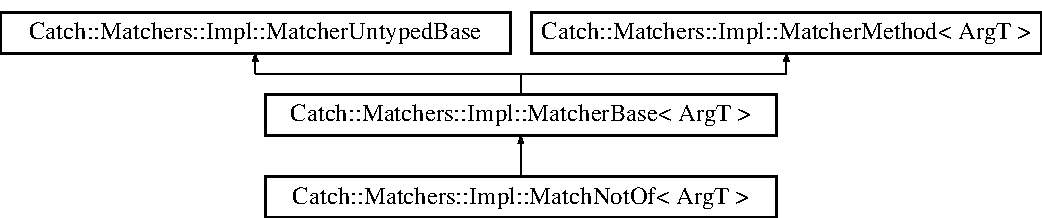
\includegraphics[height=2.926829cm]{struct_catch_1_1_matchers_1_1_impl_1_1_match_not_of}
\end{center}
\end{figure}
\subsection*{Public Member Functions}
\begin{DoxyCompactItemize}
\item 
\mbox{\hyperlink{struct_catch_1_1_matchers_1_1_impl_1_1_match_not_of_a47afdd9e4c3354cef85adc3186097ae4}{Match\+Not\+Of}} (\mbox{\hyperlink{struct_catch_1_1_matchers_1_1_impl_1_1_matcher_base}{Matcher\+Base}}$<$ ArgT $>$ const \&underlying\+Matcher)
\item 
bool \mbox{\hyperlink{struct_catch_1_1_matchers_1_1_impl_1_1_match_not_of_a181d693c0258e582d80dc6117a1f2b66}{match}} (ArgT const \&arg) const override
\item 
std\+::string \mbox{\hyperlink{struct_catch_1_1_matchers_1_1_impl_1_1_match_not_of_ac5fb4ef6a9069d23a4098c3c818f06b0}{describe}} () const override
\end{DoxyCompactItemize}
\subsection*{Public Attributes}
\begin{DoxyCompactItemize}
\item 
\mbox{\hyperlink{struct_catch_1_1_matchers_1_1_impl_1_1_matcher_base}{Matcher\+Base}}$<$ ArgT $>$ const  \& \mbox{\hyperlink{struct_catch_1_1_matchers_1_1_impl_1_1_match_not_of_af7ac67f112b0e93796b048a47329aad4}{m\+\_\+underlying\+Matcher}}
\end{DoxyCompactItemize}
\subsection*{Additional Inherited Members}


\subsection{Detailed Description}
\subsubsection*{template$<$typename ArgT$>$\newline
struct Catch\+::\+Matchers\+::\+Impl\+::\+Match\+Not\+Of$<$ Arg\+T $>$}



Definition at line 2181 of file catch.\+hpp.



\subsection{Constructor \& Destructor Documentation}
\mbox{\Hypertarget{struct_catch_1_1_matchers_1_1_impl_1_1_match_not_of_a47afdd9e4c3354cef85adc3186097ae4}\label{struct_catch_1_1_matchers_1_1_impl_1_1_match_not_of_a47afdd9e4c3354cef85adc3186097ae4}} 
\index{Catch\+::\+Matchers\+::\+Impl\+::\+Match\+Not\+Of@{Catch\+::\+Matchers\+::\+Impl\+::\+Match\+Not\+Of}!Match\+Not\+Of@{Match\+Not\+Of}}
\index{Match\+Not\+Of@{Match\+Not\+Of}!Catch\+::\+Matchers\+::\+Impl\+::\+Match\+Not\+Of@{Catch\+::\+Matchers\+::\+Impl\+::\+Match\+Not\+Of}}
\subsubsection{\texorpdfstring{Match\+Not\+Of()}{MatchNotOf()}}
{\footnotesize\ttfamily template$<$typename ArgT$>$ \\
\mbox{\hyperlink{struct_catch_1_1_matchers_1_1_impl_1_1_match_not_of}{Catch\+::\+Matchers\+::\+Impl\+::\+Match\+Not\+Of}}$<$ ArgT $>$\+::\mbox{\hyperlink{struct_catch_1_1_matchers_1_1_impl_1_1_match_not_of}{Match\+Not\+Of}} (\begin{DoxyParamCaption}\item[{\mbox{\hyperlink{struct_catch_1_1_matchers_1_1_impl_1_1_matcher_base}{Matcher\+Base}}$<$ ArgT $>$ const \&}]{underlying\+Matcher }\end{DoxyParamCaption})\hspace{0.3cm}{\ttfamily [inline]}}



Definition at line 2282 of file catch.\+hpp.



\subsection{Member Function Documentation}
\mbox{\Hypertarget{struct_catch_1_1_matchers_1_1_impl_1_1_match_not_of_ac5fb4ef6a9069d23a4098c3c818f06b0}\label{struct_catch_1_1_matchers_1_1_impl_1_1_match_not_of_ac5fb4ef6a9069d23a4098c3c818f06b0}} 
\index{Catch\+::\+Matchers\+::\+Impl\+::\+Match\+Not\+Of@{Catch\+::\+Matchers\+::\+Impl\+::\+Match\+Not\+Of}!describe@{describe}}
\index{describe@{describe}!Catch\+::\+Matchers\+::\+Impl\+::\+Match\+Not\+Of@{Catch\+::\+Matchers\+::\+Impl\+::\+Match\+Not\+Of}}
\subsubsection{\texorpdfstring{describe()}{describe()}}
{\footnotesize\ttfamily template$<$typename ArgT$>$ \\
std\+::string \mbox{\hyperlink{struct_catch_1_1_matchers_1_1_impl_1_1_match_not_of}{Catch\+::\+Matchers\+::\+Impl\+::\+Match\+Not\+Of}}$<$ ArgT $>$\+::describe (\begin{DoxyParamCaption}{ }\end{DoxyParamCaption}) const\hspace{0.3cm}{\ttfamily [inline]}, {\ttfamily [override]}, {\ttfamily [virtual]}}



Implements \mbox{\hyperlink{class_catch_1_1_matchers_1_1_impl_1_1_matcher_untyped_base_a91d3a907dbfcbb596077df24f6e11fe2}{Catch\+::\+Matchers\+::\+Impl\+::\+Matcher\+Untyped\+Base}}.



Definition at line 2288 of file catch.\+hpp.

\mbox{\Hypertarget{struct_catch_1_1_matchers_1_1_impl_1_1_match_not_of_a181d693c0258e582d80dc6117a1f2b66}\label{struct_catch_1_1_matchers_1_1_impl_1_1_match_not_of_a181d693c0258e582d80dc6117a1f2b66}} 
\index{Catch\+::\+Matchers\+::\+Impl\+::\+Match\+Not\+Of@{Catch\+::\+Matchers\+::\+Impl\+::\+Match\+Not\+Of}!match@{match}}
\index{match@{match}!Catch\+::\+Matchers\+::\+Impl\+::\+Match\+Not\+Of@{Catch\+::\+Matchers\+::\+Impl\+::\+Match\+Not\+Of}}
\subsubsection{\texorpdfstring{match()}{match()}}
{\footnotesize\ttfamily template$<$typename ArgT$>$ \\
bool \mbox{\hyperlink{struct_catch_1_1_matchers_1_1_impl_1_1_match_not_of}{Catch\+::\+Matchers\+::\+Impl\+::\+Match\+Not\+Of}}$<$ ArgT $>$\+::match (\begin{DoxyParamCaption}\item[{ArgT const \&}]{arg }\end{DoxyParamCaption}) const\hspace{0.3cm}{\ttfamily [inline]}, {\ttfamily [override]}, {\ttfamily [virtual]}}



Implements \mbox{\hyperlink{struct_catch_1_1_matchers_1_1_impl_1_1_matcher_method_ae0920ff9e817acf08e1bb0cbcb044e30}{Catch\+::\+Matchers\+::\+Impl\+::\+Matcher\+Method$<$ Arg\+T $>$}}.



Definition at line 2284 of file catch.\+hpp.



\subsection{Member Data Documentation}
\mbox{\Hypertarget{struct_catch_1_1_matchers_1_1_impl_1_1_match_not_of_af7ac67f112b0e93796b048a47329aad4}\label{struct_catch_1_1_matchers_1_1_impl_1_1_match_not_of_af7ac67f112b0e93796b048a47329aad4}} 
\index{Catch\+::\+Matchers\+::\+Impl\+::\+Match\+Not\+Of@{Catch\+::\+Matchers\+::\+Impl\+::\+Match\+Not\+Of}!m\+\_\+underlying\+Matcher@{m\+\_\+underlying\+Matcher}}
\index{m\+\_\+underlying\+Matcher@{m\+\_\+underlying\+Matcher}!Catch\+::\+Matchers\+::\+Impl\+::\+Match\+Not\+Of@{Catch\+::\+Matchers\+::\+Impl\+::\+Match\+Not\+Of}}
\subsubsection{\texorpdfstring{m\+\_\+underlying\+Matcher}{m\_underlyingMatcher}}
{\footnotesize\ttfamily template$<$typename ArgT$>$ \\
\mbox{\hyperlink{struct_catch_1_1_matchers_1_1_impl_1_1_matcher_base}{Matcher\+Base}}$<$ArgT$>$ const\& \mbox{\hyperlink{struct_catch_1_1_matchers_1_1_impl_1_1_match_not_of}{Catch\+::\+Matchers\+::\+Impl\+::\+Match\+Not\+Of}}$<$ ArgT $>$\+::m\+\_\+underlying\+Matcher}



Definition at line 2291 of file catch.\+hpp.



The documentation for this struct was generated from the following file\+:\begin{DoxyCompactItemize}
\item 
D\+:/c++/block\+\_\+matrix-\/master/block\+\_\+matrix-\/master/test/\mbox{\hyperlink{catch_8hpp}{catch.\+hpp}}\end{DoxyCompactItemize}

\hypertarget{struct_catch_1_1_message_builder}{}\section{Catch\+:\+:Message\+Builder Struct Reference}
\label{struct_catch_1_1_message_builder}\index{Catch\+::\+Message\+Builder@{Catch\+::\+Message\+Builder}}


{\ttfamily \#include $<$catch.\+hpp$>$}

Inheritance diagram for Catch\+:\+:Message\+Builder\+:\begin{figure}[H]
\begin{center}
\leavevmode
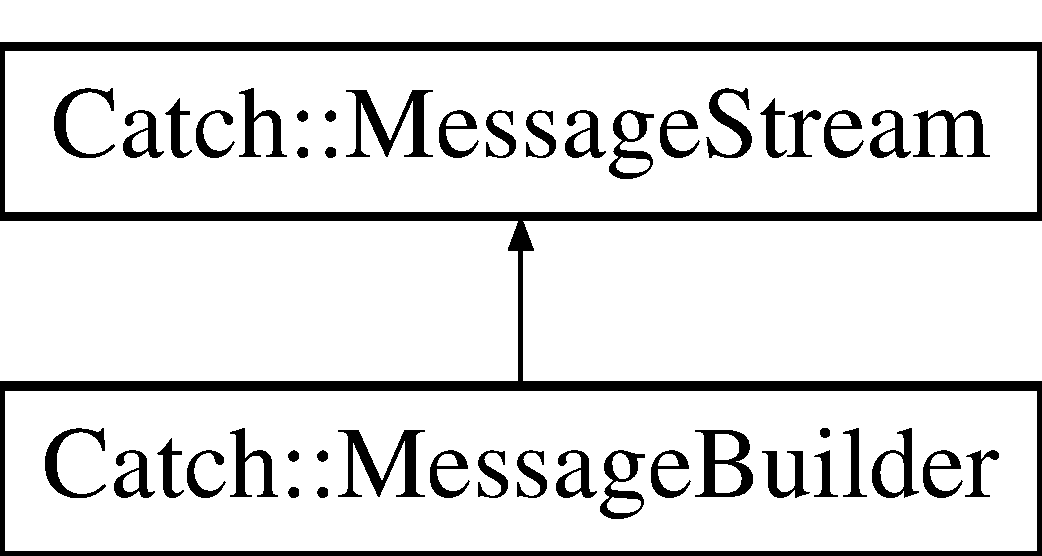
\includegraphics[height=2.000000cm]{struct_catch_1_1_message_builder}
\end{center}
\end{figure}
\subsection*{Public Member Functions}
\begin{DoxyCompactItemize}
\item 
\mbox{\hyperlink{struct_catch_1_1_message_builder_ab0c6378e722680bf58852c6ee2b6e724}{Message\+Builder}} (std\+::string const \&macro\+Name, \mbox{\hyperlink{struct_catch_1_1_source_line_info}{Source\+Line\+Info}} const \&line\+Info, \mbox{\hyperlink{struct_catch_1_1_result_was_a624e1ee3661fcf6094ceef1f654601ef}{Result\+Was\+::\+Of\+Type}} type)
\item 
{\footnotesize template$<$typename T $>$ }\\\mbox{\hyperlink{struct_catch_1_1_message_builder}{Message\+Builder}} \& \mbox{\hyperlink{struct_catch_1_1_message_builder_a20fa48d069b20dddcc2d3df8abb123c1}{operator$<$$<$}} (T const \&value)
\end{DoxyCompactItemize}
\subsection*{Public Attributes}
\begin{DoxyCompactItemize}
\item 
\mbox{\hyperlink{struct_catch_1_1_message_info}{Message\+Info}} \mbox{\hyperlink{struct_catch_1_1_message_builder_a979f1c2b36d78f80ee275bfa5ba0209f}{m\+\_\+info}}
\end{DoxyCompactItemize}


\subsection{Detailed Description}


Definition at line 1581 of file catch.\+hpp.



\subsection{Constructor \& Destructor Documentation}
\mbox{\Hypertarget{struct_catch_1_1_message_builder_ab0c6378e722680bf58852c6ee2b6e724}\label{struct_catch_1_1_message_builder_ab0c6378e722680bf58852c6ee2b6e724}} 
\index{Catch\+::\+Message\+Builder@{Catch\+::\+Message\+Builder}!Message\+Builder@{Message\+Builder}}
\index{Message\+Builder@{Message\+Builder}!Catch\+::\+Message\+Builder@{Catch\+::\+Message\+Builder}}
\subsubsection{\texorpdfstring{Message\+Builder()}{MessageBuilder()}}
{\footnotesize\ttfamily Catch\+::\+Message\+Builder\+::\+Message\+Builder (\begin{DoxyParamCaption}\item[{std\+::string const \&}]{macro\+Name,  }\item[{\mbox{\hyperlink{struct_catch_1_1_source_line_info}{Source\+Line\+Info}} const \&}]{line\+Info,  }\item[{\mbox{\hyperlink{struct_catch_1_1_result_was_a624e1ee3661fcf6094ceef1f654601ef}{Result\+Was\+::\+Of\+Type}}}]{type }\end{DoxyParamCaption})}



\subsection{Member Function Documentation}
\mbox{\Hypertarget{struct_catch_1_1_message_builder_a20fa48d069b20dddcc2d3df8abb123c1}\label{struct_catch_1_1_message_builder_a20fa48d069b20dddcc2d3df8abb123c1}} 
\index{Catch\+::\+Message\+Builder@{Catch\+::\+Message\+Builder}!operator$<$$<$@{operator$<$$<$}}
\index{operator$<$$<$@{operator$<$$<$}!Catch\+::\+Message\+Builder@{Catch\+::\+Message\+Builder}}
\subsubsection{\texorpdfstring{operator$<$$<$()}{operator<<()}}
{\footnotesize\ttfamily template$<$typename T $>$ \\
\mbox{\hyperlink{struct_catch_1_1_message_builder}{Message\+Builder}}\& Catch\+::\+Message\+Builder\+::operator$<$$<$ (\begin{DoxyParamCaption}\item[{T const \&}]{value }\end{DoxyParamCaption})\hspace{0.3cm}{\ttfamily [inline]}}



Definition at line 1587 of file catch.\+hpp.



\subsection{Member Data Documentation}
\mbox{\Hypertarget{struct_catch_1_1_message_builder_a979f1c2b36d78f80ee275bfa5ba0209f}\label{struct_catch_1_1_message_builder_a979f1c2b36d78f80ee275bfa5ba0209f}} 
\index{Catch\+::\+Message\+Builder@{Catch\+::\+Message\+Builder}!m\+\_\+info@{m\+\_\+info}}
\index{m\+\_\+info@{m\+\_\+info}!Catch\+::\+Message\+Builder@{Catch\+::\+Message\+Builder}}
\subsubsection{\texorpdfstring{m\+\_\+info}{m\_info}}
{\footnotesize\ttfamily \mbox{\hyperlink{struct_catch_1_1_message_info}{Message\+Info}} Catch\+::\+Message\+Builder\+::m\+\_\+info}



Definition at line 1592 of file catch.\+hpp.



The documentation for this struct was generated from the following file\+:\begin{DoxyCompactItemize}
\item 
D\+:/c++/block\+\_\+matrix-\/master/block\+\_\+matrix-\/master/test/\mbox{\hyperlink{catch_8hpp}{catch.\+hpp}}\end{DoxyCompactItemize}

\hypertarget{struct_catch_1_1_message_info}{}\section{Catch\+:\+:Message\+Info Struct Reference}
\label{struct_catch_1_1_message_info}\index{Catch\+::\+Message\+Info@{Catch\+::\+Message\+Info}}


{\ttfamily \#include $<$catch.\+hpp$>$}

\subsection*{Public Member Functions}
\begin{DoxyCompactItemize}
\item 
\mbox{\hyperlink{struct_catch_1_1_message_info_a2e336c33ebef7af3c1bbae6a56e14f8a}{Message\+Info}} (std\+::string const \&\+\_\+macro\+Name, \mbox{\hyperlink{struct_catch_1_1_source_line_info}{Source\+Line\+Info}} const \&\+\_\+line\+Info, \mbox{\hyperlink{struct_catch_1_1_result_was_a624e1ee3661fcf6094ceef1f654601ef}{Result\+Was\+::\+Of\+Type}} \+\_\+type)
\item 
bool \mbox{\hyperlink{struct_catch_1_1_message_info_af4b37f2172ba55395813b4bb6bbbde1a}{operator==}} (\mbox{\hyperlink{struct_catch_1_1_message_info}{Message\+Info}} const \&other) const
\item 
bool \mbox{\hyperlink{struct_catch_1_1_message_info_a8254cb8fca2da02a29a9843cdcb79df1}{operator$<$}} (\mbox{\hyperlink{struct_catch_1_1_message_info}{Message\+Info}} const \&other) const
\end{DoxyCompactItemize}
\subsection*{Public Attributes}
\begin{DoxyCompactItemize}
\item 
std\+::string \mbox{\hyperlink{struct_catch_1_1_message_info_a156ade4b3cc731f6ec7b542ae47ba8e3}{macro\+Name}}
\item 
std\+::string \mbox{\hyperlink{struct_catch_1_1_message_info_ab6cd06e050bf426c6577502a5c50e256}{message}}
\item 
\mbox{\hyperlink{struct_catch_1_1_source_line_info}{Source\+Line\+Info}} \mbox{\hyperlink{struct_catch_1_1_message_info_a985165328723e599696ebd8e43195cc5}{line\+Info}}
\item 
\mbox{\hyperlink{struct_catch_1_1_result_was_a624e1ee3661fcf6094ceef1f654601ef}{Result\+Was\+::\+Of\+Type}} \mbox{\hyperlink{struct_catch_1_1_message_info_ae928b9117465c696e45951d9d0284e78}{type}}
\item 
unsigned int \mbox{\hyperlink{struct_catch_1_1_message_info_a7f4f57ea21e50160adefce7b68a781d6}{sequence}}
\end{DoxyCompactItemize}


\subsection{Detailed Description}


Definition at line 1553 of file catch.\+hpp.



\subsection{Constructor \& Destructor Documentation}
\mbox{\Hypertarget{struct_catch_1_1_message_info_a2e336c33ebef7af3c1bbae6a56e14f8a}\label{struct_catch_1_1_message_info_a2e336c33ebef7af3c1bbae6a56e14f8a}} 
\index{Catch\+::\+Message\+Info@{Catch\+::\+Message\+Info}!Message\+Info@{Message\+Info}}
\index{Message\+Info@{Message\+Info}!Catch\+::\+Message\+Info@{Catch\+::\+Message\+Info}}
\subsubsection{\texorpdfstring{Message\+Info()}{MessageInfo()}}
{\footnotesize\ttfamily Catch\+::\+Message\+Info\+::\+Message\+Info (\begin{DoxyParamCaption}\item[{std\+::string const \&}]{\+\_\+macro\+Name,  }\item[{\mbox{\hyperlink{struct_catch_1_1_source_line_info}{Source\+Line\+Info}} const \&}]{\+\_\+line\+Info,  }\item[{\mbox{\hyperlink{struct_catch_1_1_result_was_a624e1ee3661fcf6094ceef1f654601ef}{Result\+Was\+::\+Of\+Type}}}]{\+\_\+type }\end{DoxyParamCaption})}



\subsection{Member Function Documentation}
\mbox{\Hypertarget{struct_catch_1_1_message_info_a8254cb8fca2da02a29a9843cdcb79df1}\label{struct_catch_1_1_message_info_a8254cb8fca2da02a29a9843cdcb79df1}} 
\index{Catch\+::\+Message\+Info@{Catch\+::\+Message\+Info}!operator$<$@{operator$<$}}
\index{operator$<$@{operator$<$}!Catch\+::\+Message\+Info@{Catch\+::\+Message\+Info}}
\subsubsection{\texorpdfstring{operator$<$()}{operator<()}}
{\footnotesize\ttfamily bool Catch\+::\+Message\+Info\+::operator$<$ (\begin{DoxyParamCaption}\item[{\mbox{\hyperlink{struct_catch_1_1_message_info}{Message\+Info}} const \&}]{other }\end{DoxyParamCaption}) const}

\mbox{\Hypertarget{struct_catch_1_1_message_info_af4b37f2172ba55395813b4bb6bbbde1a}\label{struct_catch_1_1_message_info_af4b37f2172ba55395813b4bb6bbbde1a}} 
\index{Catch\+::\+Message\+Info@{Catch\+::\+Message\+Info}!operator==@{operator==}}
\index{operator==@{operator==}!Catch\+::\+Message\+Info@{Catch\+::\+Message\+Info}}
\subsubsection{\texorpdfstring{operator==()}{operator==()}}
{\footnotesize\ttfamily bool Catch\+::\+Message\+Info\+::operator== (\begin{DoxyParamCaption}\item[{\mbox{\hyperlink{struct_catch_1_1_message_info}{Message\+Info}} const \&}]{other }\end{DoxyParamCaption}) const}



\subsection{Member Data Documentation}
\mbox{\Hypertarget{struct_catch_1_1_message_info_a985165328723e599696ebd8e43195cc5}\label{struct_catch_1_1_message_info_a985165328723e599696ebd8e43195cc5}} 
\index{Catch\+::\+Message\+Info@{Catch\+::\+Message\+Info}!line\+Info@{line\+Info}}
\index{line\+Info@{line\+Info}!Catch\+::\+Message\+Info@{Catch\+::\+Message\+Info}}
\subsubsection{\texorpdfstring{line\+Info}{lineInfo}}
{\footnotesize\ttfamily \mbox{\hyperlink{struct_catch_1_1_source_line_info}{Source\+Line\+Info}} Catch\+::\+Message\+Info\+::line\+Info}



Definition at line 1560 of file catch.\+hpp.

\mbox{\Hypertarget{struct_catch_1_1_message_info_a156ade4b3cc731f6ec7b542ae47ba8e3}\label{struct_catch_1_1_message_info_a156ade4b3cc731f6ec7b542ae47ba8e3}} 
\index{Catch\+::\+Message\+Info@{Catch\+::\+Message\+Info}!macro\+Name@{macro\+Name}}
\index{macro\+Name@{macro\+Name}!Catch\+::\+Message\+Info@{Catch\+::\+Message\+Info}}
\subsubsection{\texorpdfstring{macro\+Name}{macroName}}
{\footnotesize\ttfamily std\+::string Catch\+::\+Message\+Info\+::macro\+Name}



Definition at line 1558 of file catch.\+hpp.

\mbox{\Hypertarget{struct_catch_1_1_message_info_ab6cd06e050bf426c6577502a5c50e256}\label{struct_catch_1_1_message_info_ab6cd06e050bf426c6577502a5c50e256}} 
\index{Catch\+::\+Message\+Info@{Catch\+::\+Message\+Info}!message@{message}}
\index{message@{message}!Catch\+::\+Message\+Info@{Catch\+::\+Message\+Info}}
\subsubsection{\texorpdfstring{message}{message}}
{\footnotesize\ttfamily std\+::string Catch\+::\+Message\+Info\+::message}



Definition at line 1559 of file catch.\+hpp.

\mbox{\Hypertarget{struct_catch_1_1_message_info_a7f4f57ea21e50160adefce7b68a781d6}\label{struct_catch_1_1_message_info_a7f4f57ea21e50160adefce7b68a781d6}} 
\index{Catch\+::\+Message\+Info@{Catch\+::\+Message\+Info}!sequence@{sequence}}
\index{sequence@{sequence}!Catch\+::\+Message\+Info@{Catch\+::\+Message\+Info}}
\subsubsection{\texorpdfstring{sequence}{sequence}}
{\footnotesize\ttfamily unsigned int Catch\+::\+Message\+Info\+::sequence}



Definition at line 1562 of file catch.\+hpp.

\mbox{\Hypertarget{struct_catch_1_1_message_info_ae928b9117465c696e45951d9d0284e78}\label{struct_catch_1_1_message_info_ae928b9117465c696e45951d9d0284e78}} 
\index{Catch\+::\+Message\+Info@{Catch\+::\+Message\+Info}!type@{type}}
\index{type@{type}!Catch\+::\+Message\+Info@{Catch\+::\+Message\+Info}}
\subsubsection{\texorpdfstring{type}{type}}
{\footnotesize\ttfamily \mbox{\hyperlink{struct_catch_1_1_result_was_a624e1ee3661fcf6094ceef1f654601ef}{Result\+Was\+::\+Of\+Type}} Catch\+::\+Message\+Info\+::type}



Definition at line 1561 of file catch.\+hpp.



The documentation for this struct was generated from the following file\+:\begin{DoxyCompactItemize}
\item 
D\+:/c++/block\+\_\+matrix-\/master/block\+\_\+matrix-\/master/test/\mbox{\hyperlink{catch_8hpp}{catch.\+hpp}}\end{DoxyCompactItemize}

\hypertarget{struct_catch_1_1_message_stream}{}\section{Catch\+:\+:Message\+Stream Struct Reference}
\label{struct_catch_1_1_message_stream}\index{Catch\+::\+Message\+Stream@{Catch\+::\+Message\+Stream}}


{\ttfamily \#include $<$catch.\+hpp$>$}

Inheritance diagram for Catch\+:\+:Message\+Stream\+:\begin{figure}[H]
\begin{center}
\leavevmode
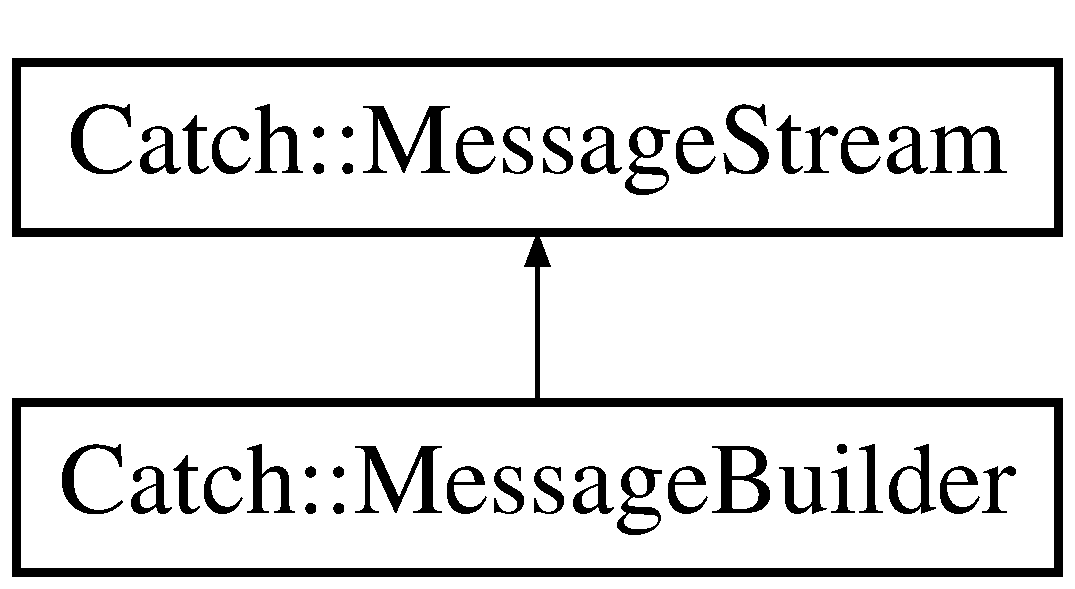
\includegraphics[height=2.000000cm]{struct_catch_1_1_message_stream}
\end{center}
\end{figure}
\subsection*{Public Member Functions}
\begin{DoxyCompactItemize}
\item 
{\footnotesize template$<$typename T $>$ }\\\mbox{\hyperlink{struct_catch_1_1_message_stream}{Message\+Stream}} \& \mbox{\hyperlink{struct_catch_1_1_message_stream_a554c4aff5925a077e9fe9d858217428d}{operator$<$$<$}} (T const \&value)
\end{DoxyCompactItemize}
\subsection*{Public Attributes}
\begin{DoxyCompactItemize}
\item 
\mbox{\hyperlink{class_catch_1_1_reusable_string_stream}{Reusable\+String\+Stream}} \mbox{\hyperlink{struct_catch_1_1_message_stream_a9202520faed8882ef469db9f353ec578}{m\+\_\+stream}}
\end{DoxyCompactItemize}


\subsection{Detailed Description}


Definition at line 1570 of file catch.\+hpp.



\subsection{Member Function Documentation}
\mbox{\Hypertarget{struct_catch_1_1_message_stream_a554c4aff5925a077e9fe9d858217428d}\label{struct_catch_1_1_message_stream_a554c4aff5925a077e9fe9d858217428d}} 
\index{Catch\+::\+Message\+Stream@{Catch\+::\+Message\+Stream}!operator$<$$<$@{operator$<$$<$}}
\index{operator$<$$<$@{operator$<$$<$}!Catch\+::\+Message\+Stream@{Catch\+::\+Message\+Stream}}
\subsubsection{\texorpdfstring{operator$<$$<$()}{operator<<()}}
{\footnotesize\ttfamily template$<$typename T $>$ \\
\mbox{\hyperlink{struct_catch_1_1_message_stream}{Message\+Stream}}\& Catch\+::\+Message\+Stream\+::operator$<$$<$ (\begin{DoxyParamCaption}\item[{T const \&}]{value }\end{DoxyParamCaption})\hspace{0.3cm}{\ttfamily [inline]}}



Definition at line 1573 of file catch.\+hpp.



\subsection{Member Data Documentation}
\mbox{\Hypertarget{struct_catch_1_1_message_stream_a9202520faed8882ef469db9f353ec578}\label{struct_catch_1_1_message_stream_a9202520faed8882ef469db9f353ec578}} 
\index{Catch\+::\+Message\+Stream@{Catch\+::\+Message\+Stream}!m\+\_\+stream@{m\+\_\+stream}}
\index{m\+\_\+stream@{m\+\_\+stream}!Catch\+::\+Message\+Stream@{Catch\+::\+Message\+Stream}}
\subsubsection{\texorpdfstring{m\+\_\+stream}{m\_stream}}
{\footnotesize\ttfamily \mbox{\hyperlink{class_catch_1_1_reusable_string_stream}{Reusable\+String\+Stream}} Catch\+::\+Message\+Stream\+::m\+\_\+stream}



Definition at line 1578 of file catch.\+hpp.



The documentation for this struct was generated from the following file\+:\begin{DoxyCompactItemize}
\item 
D\+:/c++/block\+\_\+matrix-\/master/block\+\_\+matrix-\/master/test/\mbox{\hyperlink{catch_8hpp}{catch.\+hpp}}\end{DoxyCompactItemize}

\hypertarget{struct_catch_1_1_name_and_tags}{}\section{Catch\+:\+:Name\+And\+Tags Struct Reference}
\label{struct_catch_1_1_name_and_tags}\index{Catch\+::\+Name\+And\+Tags@{Catch\+::\+Name\+And\+Tags}}


{\ttfamily \#include $<$catch.\+hpp$>$}

\subsection*{Public Member Functions}
\begin{DoxyCompactItemize}
\item 
\mbox{\hyperlink{struct_catch_1_1_name_and_tags_ab585111e615ce8c504a2b9630de8ee94}{Name\+And\+Tags}} (\mbox{\hyperlink{class_catch_1_1_string_ref}{String\+Ref}} const \&name\+\_\+=\mbox{\hyperlink{class_catch_1_1_string_ref}{String\+Ref}}(), \mbox{\hyperlink{class_catch_1_1_string_ref}{String\+Ref}} const \&tags\+\_\+=\mbox{\hyperlink{class_catch_1_1_string_ref}{String\+Ref}}()) noexcept
\end{DoxyCompactItemize}
\subsection*{Public Attributes}
\begin{DoxyCompactItemize}
\item 
\mbox{\hyperlink{class_catch_1_1_string_ref}{String\+Ref}} \mbox{\hyperlink{struct_catch_1_1_name_and_tags_a7cbea60e0cebfa622c667008eb011420}{name}}
\item 
\mbox{\hyperlink{class_catch_1_1_string_ref}{String\+Ref}} \mbox{\hyperlink{struct_catch_1_1_name_and_tags_a74062ed1138834a348424eb7ed900c57}{tags}}
\end{DoxyCompactItemize}


\subsection{Detailed Description}


Definition at line 503 of file catch.\+hpp.



\subsection{Constructor \& Destructor Documentation}
\mbox{\Hypertarget{struct_catch_1_1_name_and_tags_ab585111e615ce8c504a2b9630de8ee94}\label{struct_catch_1_1_name_and_tags_ab585111e615ce8c504a2b9630de8ee94}} 
\index{Catch\+::\+Name\+And\+Tags@{Catch\+::\+Name\+And\+Tags}!Name\+And\+Tags@{Name\+And\+Tags}}
\index{Name\+And\+Tags@{Name\+And\+Tags}!Catch\+::\+Name\+And\+Tags@{Catch\+::\+Name\+And\+Tags}}
\subsubsection{\texorpdfstring{Name\+And\+Tags()}{NameAndTags()}}
{\footnotesize\ttfamily Catch\+::\+Name\+And\+Tags\+::\+Name\+And\+Tags (\begin{DoxyParamCaption}\item[{\mbox{\hyperlink{class_catch_1_1_string_ref}{String\+Ref}} const \&}]{name\+\_\+ = {\ttfamily \mbox{\hyperlink{class_catch_1_1_string_ref}{String\+Ref}}()},  }\item[{\mbox{\hyperlink{class_catch_1_1_string_ref}{String\+Ref}} const \&}]{tags\+\_\+ = {\ttfamily \mbox{\hyperlink{class_catch_1_1_string_ref}{String\+Ref}}()} }\end{DoxyParamCaption})\hspace{0.3cm}{\ttfamily [noexcept]}}



\subsection{Member Data Documentation}
\mbox{\Hypertarget{struct_catch_1_1_name_and_tags_a7cbea60e0cebfa622c667008eb011420}\label{struct_catch_1_1_name_and_tags_a7cbea60e0cebfa622c667008eb011420}} 
\index{Catch\+::\+Name\+And\+Tags@{Catch\+::\+Name\+And\+Tags}!name@{name}}
\index{name@{name}!Catch\+::\+Name\+And\+Tags@{Catch\+::\+Name\+And\+Tags}}
\subsubsection{\texorpdfstring{name}{name}}
{\footnotesize\ttfamily \mbox{\hyperlink{class_catch_1_1_string_ref}{String\+Ref}} Catch\+::\+Name\+And\+Tags\+::name}



Definition at line 505 of file catch.\+hpp.

\mbox{\Hypertarget{struct_catch_1_1_name_and_tags_a74062ed1138834a348424eb7ed900c57}\label{struct_catch_1_1_name_and_tags_a74062ed1138834a348424eb7ed900c57}} 
\index{Catch\+::\+Name\+And\+Tags@{Catch\+::\+Name\+And\+Tags}!tags@{tags}}
\index{tags@{tags}!Catch\+::\+Name\+And\+Tags@{Catch\+::\+Name\+And\+Tags}}
\subsubsection{\texorpdfstring{tags}{tags}}
{\footnotesize\ttfamily \mbox{\hyperlink{class_catch_1_1_string_ref}{String\+Ref}} Catch\+::\+Name\+And\+Tags\+::tags}



Definition at line 506 of file catch.\+hpp.



The documentation for this struct was generated from the following file\+:\begin{DoxyCompactItemize}
\item 
D\+:/c++/block\+\_\+matrix-\/master/block\+\_\+matrix-\/master/test/\mbox{\hyperlink{catch_8hpp}{catch.\+hpp}}\end{DoxyCompactItemize}

\hypertarget{class_catch_1_1_non_copyable}{}\section{Catch\+:\+:Non\+Copyable Class Reference}
\label{class_catch_1_1_non_copyable}\index{Catch\+::\+Non\+Copyable@{Catch\+::\+Non\+Copyable}}


{\ttfamily \#include $<$catch.\+hpp$>$}

Inheritance diagram for Catch\+:\+:Non\+Copyable\+:\begin{figure}[H]
\begin{center}
\leavevmode
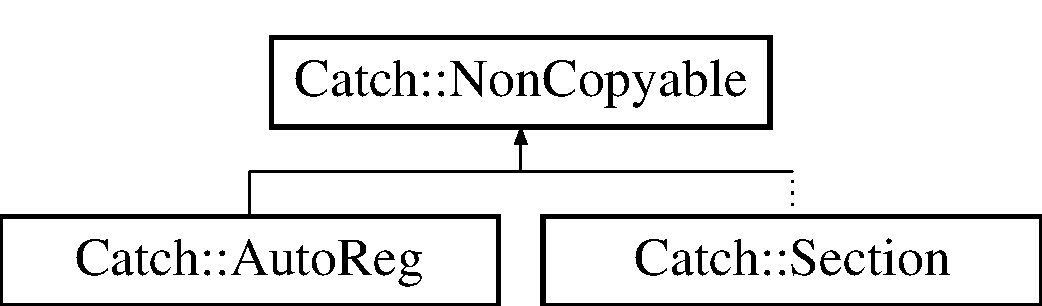
\includegraphics[height=2.000000cm]{class_catch_1_1_non_copyable}
\end{center}
\end{figure}
\subsection*{Protected Member Functions}
\begin{DoxyCompactItemize}
\item 
\mbox{\hyperlink{class_catch_1_1_non_copyable_a4b492dd5753f9952350fb64dc6cb9fe2}{Non\+Copyable}} ()
\item 
virtual \mbox{\hyperlink{class_catch_1_1_non_copyable_a81254677280fef337eb4a676e91e3293}{$\sim$\+Non\+Copyable}} ()
\end{DoxyCompactItemize}


\subsection{Detailed Description}


Definition at line 261 of file catch.\+hpp.



\subsection{Constructor \& Destructor Documentation}
\mbox{\Hypertarget{class_catch_1_1_non_copyable_a4b492dd5753f9952350fb64dc6cb9fe2}\label{class_catch_1_1_non_copyable_a4b492dd5753f9952350fb64dc6cb9fe2}} 
\index{Catch\+::\+Non\+Copyable@{Catch\+::\+Non\+Copyable}!Non\+Copyable@{Non\+Copyable}}
\index{Non\+Copyable@{Non\+Copyable}!Catch\+::\+Non\+Copyable@{Catch\+::\+Non\+Copyable}}
\subsubsection{\texorpdfstring{Non\+Copyable()}{NonCopyable()}}
{\footnotesize\ttfamily Catch\+::\+Non\+Copyable\+::\+Non\+Copyable (\begin{DoxyParamCaption}{ }\end{DoxyParamCaption})\hspace{0.3cm}{\ttfamily [protected]}}

\mbox{\Hypertarget{class_catch_1_1_non_copyable_a81254677280fef337eb4a676e91e3293}\label{class_catch_1_1_non_copyable_a81254677280fef337eb4a676e91e3293}} 
\index{Catch\+::\+Non\+Copyable@{Catch\+::\+Non\+Copyable}!````~Non\+Copyable@{$\sim$\+Non\+Copyable}}
\index{````~Non\+Copyable@{$\sim$\+Non\+Copyable}!Catch\+::\+Non\+Copyable@{Catch\+::\+Non\+Copyable}}
\subsubsection{\texorpdfstring{$\sim$\+Non\+Copyable()}{~NonCopyable()}}
{\footnotesize\ttfamily virtual Catch\+::\+Non\+Copyable\+::$\sim$\+Non\+Copyable (\begin{DoxyParamCaption}{ }\end{DoxyParamCaption})\hspace{0.3cm}{\ttfamily [protected]}, {\ttfamily [virtual]}}



The documentation for this class was generated from the following file\+:\begin{DoxyCompactItemize}
\item 
D\+:/c++/block\+\_\+matrix-\/master/block\+\_\+matrix-\/master/test/\mbox{\hyperlink{catch_8hpp}{catch.\+hpp}}\end{DoxyCompactItemize}

\hypertarget{struct_catch_1_1not__this__one}{}\section{Catch\+:\+:not\+\_\+this\+\_\+one Struct Reference}
\label{struct_catch_1_1not__this__one}\index{Catch\+::not\+\_\+this\+\_\+one@{Catch\+::not\+\_\+this\+\_\+one}}


{\ttfamily \#include $<$catch.\+hpp$>$}



\subsection{Detailed Description}


Definition at line 1067 of file catch.\+hpp.



The documentation for this struct was generated from the following file\+:\begin{DoxyCompactItemize}
\item 
D\+:/c++/block\+\_\+matrix-\/master/block\+\_\+matrix-\/master/test/\mbox{\hyperlink{catch_8hpp}{catch.\+hpp}}\end{DoxyCompactItemize}

\hypertarget{struct_catch_1_1pluralise}{}\section{Catch\+:\+:pluralise Struct Reference}
\label{struct_catch_1_1pluralise}\index{Catch\+::pluralise@{Catch\+::pluralise}}


{\ttfamily \#include $<$catch.\+hpp$>$}

\subsection*{Public Member Functions}
\begin{DoxyCompactItemize}
\item 
\mbox{\hyperlink{struct_catch_1_1pluralise_a5c55e22de2416cfe416edf715c6b9234}{pluralise}} (std\+::size\+\_\+t count, std\+::string const \&label)
\end{DoxyCompactItemize}
\subsection*{Public Attributes}
\begin{DoxyCompactItemize}
\item 
std\+::size\+\_\+t \mbox{\hyperlink{struct_catch_1_1pluralise_a4dce2fa13ec6f00fac09b2418265441e}{m\+\_\+count}}
\item 
std\+::string \mbox{\hyperlink{struct_catch_1_1pluralise_a8849cbdd3f11ebe7747597c8644e8793}{m\+\_\+label}}
\end{DoxyCompactItemize}
\subsection*{Friends}
\begin{DoxyCompactItemize}
\item 
std\+::ostream \& \mbox{\hyperlink{struct_catch_1_1pluralise_aa7dac6b165514c1f85e0695d678fdef5}{operator$<$$<$}} (std\+::ostream \&os, \mbox{\hyperlink{struct_catch_1_1pluralise}{pluralise}} const \&pluraliser)
\end{DoxyCompactItemize}


\subsection{Detailed Description}


Definition at line 2156 of file catch.\+hpp.



\subsection{Constructor \& Destructor Documentation}
\mbox{\Hypertarget{struct_catch_1_1pluralise_a5c55e22de2416cfe416edf715c6b9234}\label{struct_catch_1_1pluralise_a5c55e22de2416cfe416edf715c6b9234}} 
\index{Catch\+::pluralise@{Catch\+::pluralise}!pluralise@{pluralise}}
\index{pluralise@{pluralise}!Catch\+::pluralise@{Catch\+::pluralise}}
\subsubsection{\texorpdfstring{pluralise()}{pluralise()}}
{\footnotesize\ttfamily Catch\+::pluralise\+::pluralise (\begin{DoxyParamCaption}\item[{std\+::size\+\_\+t}]{count,  }\item[{std\+::string const \&}]{label }\end{DoxyParamCaption})}



\subsection{Friends And Related Function Documentation}
\mbox{\Hypertarget{struct_catch_1_1pluralise_aa7dac6b165514c1f85e0695d678fdef5}\label{struct_catch_1_1pluralise_aa7dac6b165514c1f85e0695d678fdef5}} 
\index{Catch\+::pluralise@{Catch\+::pluralise}!operator$<$$<$@{operator$<$$<$}}
\index{operator$<$$<$@{operator$<$$<$}!Catch\+::pluralise@{Catch\+::pluralise}}
\subsubsection{\texorpdfstring{operator$<$$<$}{operator<<}}
{\footnotesize\ttfamily std\+::ostream\& operator$<$$<$ (\begin{DoxyParamCaption}\item[{std\+::ostream \&}]{os,  }\item[{\mbox{\hyperlink{struct_catch_1_1pluralise}{pluralise}} const \&}]{pluraliser }\end{DoxyParamCaption})\hspace{0.3cm}{\ttfamily [friend]}}



\subsection{Member Data Documentation}
\mbox{\Hypertarget{struct_catch_1_1pluralise_a4dce2fa13ec6f00fac09b2418265441e}\label{struct_catch_1_1pluralise_a4dce2fa13ec6f00fac09b2418265441e}} 
\index{Catch\+::pluralise@{Catch\+::pluralise}!m\+\_\+count@{m\+\_\+count}}
\index{m\+\_\+count@{m\+\_\+count}!Catch\+::pluralise@{Catch\+::pluralise}}
\subsubsection{\texorpdfstring{m\+\_\+count}{m\_count}}
{\footnotesize\ttfamily std\+::size\+\_\+t Catch\+::pluralise\+::m\+\_\+count}



Definition at line 2161 of file catch.\+hpp.

\mbox{\Hypertarget{struct_catch_1_1pluralise_a8849cbdd3f11ebe7747597c8644e8793}\label{struct_catch_1_1pluralise_a8849cbdd3f11ebe7747597c8644e8793}} 
\index{Catch\+::pluralise@{Catch\+::pluralise}!m\+\_\+label@{m\+\_\+label}}
\index{m\+\_\+label@{m\+\_\+label}!Catch\+::pluralise@{Catch\+::pluralise}}
\subsubsection{\texorpdfstring{m\+\_\+label}{m\_label}}
{\footnotesize\ttfamily std\+::string Catch\+::pluralise\+::m\+\_\+label}



Definition at line 2162 of file catch.\+hpp.



The documentation for this struct was generated from the following file\+:\begin{DoxyCompactItemize}
\item 
D\+:/c++/block\+\_\+matrix-\/master/block\+\_\+matrix-\/master/test/\mbox{\hyperlink{catch_8hpp}{catch.\+hpp}}\end{DoxyCompactItemize}

\hypertarget{struct_catch_1_1_matchers_1_1_std_string_1_1_regex_matcher}{}\section{Catch\+:\+:Matchers\+:\+:Std\+String\+:\+:Regex\+Matcher Struct Reference}
\label{struct_catch_1_1_matchers_1_1_std_string_1_1_regex_matcher}\index{Catch\+::\+Matchers\+::\+Std\+String\+::\+Regex\+Matcher@{Catch\+::\+Matchers\+::\+Std\+String\+::\+Regex\+Matcher}}


{\ttfamily \#include $<$catch.\+hpp$>$}

Inheritance diagram for Catch\+:\+:Matchers\+:\+:Std\+String\+:\+:Regex\+Matcher\+:\begin{figure}[H]
\begin{center}
\leavevmode
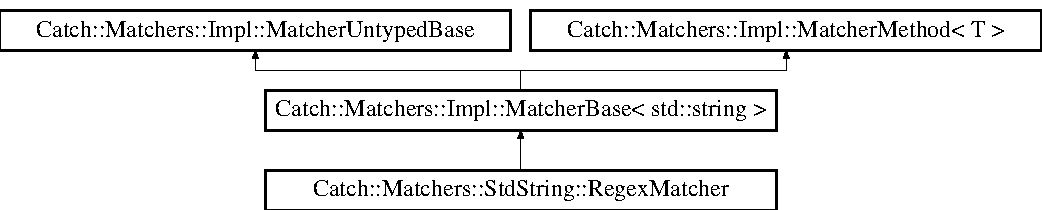
\includegraphics[height=2.818792cm]{struct_catch_1_1_matchers_1_1_std_string_1_1_regex_matcher}
\end{center}
\end{figure}
\subsection*{Public Member Functions}
\begin{DoxyCompactItemize}
\item 
\mbox{\hyperlink{struct_catch_1_1_matchers_1_1_std_string_1_1_regex_matcher_ab914deb885fe25558c41ab368c6b3916}{Regex\+Matcher}} (std\+::string regex, \mbox{\hyperlink{struct_catch_1_1_case_sensitive_aad49d3aee2d97066642fffa919685c6a}{Case\+Sensitive\+::\+Choice}} case\+Sensitivity)
\item 
bool \mbox{\hyperlink{struct_catch_1_1_matchers_1_1_std_string_1_1_regex_matcher_aa8e61adccabb2f36133029301f6b8f4e}{match}} (std\+::string const \&matchee) const override
\item 
std\+::string \mbox{\hyperlink{struct_catch_1_1_matchers_1_1_std_string_1_1_regex_matcher_a1f788cd5258c987e5043f6c7f43adeb9}{describe}} () const override
\end{DoxyCompactItemize}
\subsection*{Additional Inherited Members}


\subsection{Detailed Description}


Definition at line 2404 of file catch.\+hpp.



\subsection{Constructor \& Destructor Documentation}
\mbox{\Hypertarget{struct_catch_1_1_matchers_1_1_std_string_1_1_regex_matcher_ab914deb885fe25558c41ab368c6b3916}\label{struct_catch_1_1_matchers_1_1_std_string_1_1_regex_matcher_ab914deb885fe25558c41ab368c6b3916}} 
\index{Catch\+::\+Matchers\+::\+Std\+String\+::\+Regex\+Matcher@{Catch\+::\+Matchers\+::\+Std\+String\+::\+Regex\+Matcher}!Regex\+Matcher@{Regex\+Matcher}}
\index{Regex\+Matcher@{Regex\+Matcher}!Catch\+::\+Matchers\+::\+Std\+String\+::\+Regex\+Matcher@{Catch\+::\+Matchers\+::\+Std\+String\+::\+Regex\+Matcher}}
\subsubsection{\texorpdfstring{Regex\+Matcher()}{RegexMatcher()}}
{\footnotesize\ttfamily Catch\+::\+Matchers\+::\+Std\+String\+::\+Regex\+Matcher\+::\+Regex\+Matcher (\begin{DoxyParamCaption}\item[{std\+::string}]{regex,  }\item[{\mbox{\hyperlink{struct_catch_1_1_case_sensitive_aad49d3aee2d97066642fffa919685c6a}{Case\+Sensitive\+::\+Choice}}}]{case\+Sensitivity }\end{DoxyParamCaption})}



\subsection{Member Function Documentation}
\mbox{\Hypertarget{struct_catch_1_1_matchers_1_1_std_string_1_1_regex_matcher_a1f788cd5258c987e5043f6c7f43adeb9}\label{struct_catch_1_1_matchers_1_1_std_string_1_1_regex_matcher_a1f788cd5258c987e5043f6c7f43adeb9}} 
\index{Catch\+::\+Matchers\+::\+Std\+String\+::\+Regex\+Matcher@{Catch\+::\+Matchers\+::\+Std\+String\+::\+Regex\+Matcher}!describe@{describe}}
\index{describe@{describe}!Catch\+::\+Matchers\+::\+Std\+String\+::\+Regex\+Matcher@{Catch\+::\+Matchers\+::\+Std\+String\+::\+Regex\+Matcher}}
\subsubsection{\texorpdfstring{describe()}{describe()}}
{\footnotesize\ttfamily std\+::string Catch\+::\+Matchers\+::\+Std\+String\+::\+Regex\+Matcher\+::describe (\begin{DoxyParamCaption}{ }\end{DoxyParamCaption}) const\hspace{0.3cm}{\ttfamily [override]}, {\ttfamily [virtual]}}



Implements \mbox{\hyperlink{class_catch_1_1_matchers_1_1_impl_1_1_matcher_untyped_base_a91d3a907dbfcbb596077df24f6e11fe2}{Catch\+::\+Matchers\+::\+Impl\+::\+Matcher\+Untyped\+Base}}.

\mbox{\Hypertarget{struct_catch_1_1_matchers_1_1_std_string_1_1_regex_matcher_aa8e61adccabb2f36133029301f6b8f4e}\label{struct_catch_1_1_matchers_1_1_std_string_1_1_regex_matcher_aa8e61adccabb2f36133029301f6b8f4e}} 
\index{Catch\+::\+Matchers\+::\+Std\+String\+::\+Regex\+Matcher@{Catch\+::\+Matchers\+::\+Std\+String\+::\+Regex\+Matcher}!match@{match}}
\index{match@{match}!Catch\+::\+Matchers\+::\+Std\+String\+::\+Regex\+Matcher@{Catch\+::\+Matchers\+::\+Std\+String\+::\+Regex\+Matcher}}
\subsubsection{\texorpdfstring{match()}{match()}}
{\footnotesize\ttfamily bool Catch\+::\+Matchers\+::\+Std\+String\+::\+Regex\+Matcher\+::match (\begin{DoxyParamCaption}\item[{std\+::string const \&}]{matchee }\end{DoxyParamCaption}) const\hspace{0.3cm}{\ttfamily [override]}}



The documentation for this struct was generated from the following file\+:\begin{DoxyCompactItemize}
\item 
D\+:/c++/block\+\_\+matrix-\/master/block\+\_\+matrix-\/master/test/\mbox{\hyperlink{catch_8hpp}{catch.\+hpp}}\end{DoxyCompactItemize}

\hypertarget{struct_catch_1_1_registrar_for_tag_aliases}{}\section{Catch\+:\+:Registrar\+For\+Tag\+Aliases Struct Reference}
\label{struct_catch_1_1_registrar_for_tag_aliases}\index{Catch\+::\+Registrar\+For\+Tag\+Aliases@{Catch\+::\+Registrar\+For\+Tag\+Aliases}}


{\ttfamily \#include $<$catch.\+hpp$>$}

\subsection*{Public Member Functions}
\begin{DoxyCompactItemize}
\item 
\mbox{\hyperlink{struct_catch_1_1_registrar_for_tag_aliases_ae4e45830e4763bcd65d55d8db9167b69}{Registrar\+For\+Tag\+Aliases}} (char const $\ast$alias, char const $\ast$tag, \mbox{\hyperlink{struct_catch_1_1_source_line_info}{Source\+Line\+Info}} const \&line\+Info)
\end{DoxyCompactItemize}


\subsection{Detailed Description}


Definition at line 314 of file catch.\+hpp.



\subsection{Constructor \& Destructor Documentation}
\mbox{\Hypertarget{struct_catch_1_1_registrar_for_tag_aliases_ae4e45830e4763bcd65d55d8db9167b69}\label{struct_catch_1_1_registrar_for_tag_aliases_ae4e45830e4763bcd65d55d8db9167b69}} 
\index{Catch\+::\+Registrar\+For\+Tag\+Aliases@{Catch\+::\+Registrar\+For\+Tag\+Aliases}!Registrar\+For\+Tag\+Aliases@{Registrar\+For\+Tag\+Aliases}}
\index{Registrar\+For\+Tag\+Aliases@{Registrar\+For\+Tag\+Aliases}!Catch\+::\+Registrar\+For\+Tag\+Aliases@{Catch\+::\+Registrar\+For\+Tag\+Aliases}}
\subsubsection{\texorpdfstring{Registrar\+For\+Tag\+Aliases()}{RegistrarForTagAliases()}}
{\footnotesize\ttfamily Catch\+::\+Registrar\+For\+Tag\+Aliases\+::\+Registrar\+For\+Tag\+Aliases (\begin{DoxyParamCaption}\item[{char const $\ast$}]{alias,  }\item[{char const $\ast$}]{tag,  }\item[{\mbox{\hyperlink{struct_catch_1_1_source_line_info}{Source\+Line\+Info}} const \&}]{line\+Info }\end{DoxyParamCaption})}



The documentation for this struct was generated from the following file\+:\begin{DoxyCompactItemize}
\item 
D\+:/c++/block\+\_\+matrix-\/master/block\+\_\+matrix-\/master/test/\mbox{\hyperlink{catch_8hpp}{catch.\+hpp}}\end{DoxyCompactItemize}

\hypertarget{struct_catch_1_1_result_disposition}{}\section{Catch\+:\+:Result\+Disposition Struct Reference}
\label{struct_catch_1_1_result_disposition}\index{Catch\+::\+Result\+Disposition@{Catch\+::\+Result\+Disposition}}


{\ttfamily \#include $<$catch.\+hpp$>$}

\subsection*{Public Types}
\begin{DoxyCompactItemize}
\item 
enum \mbox{\hyperlink{struct_catch_1_1_result_disposition_a3396cad6e2259af326b3aae93e23e9d8}{Flags}} \{ \mbox{\hyperlink{struct_catch_1_1_result_disposition_a3396cad6e2259af326b3aae93e23e9d8af3bd52347ed6f8796e8ce2f77bb39ea5}{Normal}} = 0x01, 
\mbox{\hyperlink{struct_catch_1_1_result_disposition_a3396cad6e2259af326b3aae93e23e9d8aa18c94bd60c5614e17a84c2ced3bbfd5}{Continue\+On\+Failure}} = 0x02, 
\mbox{\hyperlink{struct_catch_1_1_result_disposition_a3396cad6e2259af326b3aae93e23e9d8a9980604245f19884691f941dec03eeb8}{False\+Test}} = 0x04, 
\mbox{\hyperlink{struct_catch_1_1_result_disposition_a3396cad6e2259af326b3aae93e23e9d8a1a88eb6004bddee4ccae4b421991bf54}{Suppress\+Fail}} = 0x08
 \}
\end{DoxyCompactItemize}


\subsection{Detailed Description}


Definition at line 601 of file catch.\+hpp.



\subsection{Member Enumeration Documentation}
\mbox{\Hypertarget{struct_catch_1_1_result_disposition_a3396cad6e2259af326b3aae93e23e9d8}\label{struct_catch_1_1_result_disposition_a3396cad6e2259af326b3aae93e23e9d8}} 
\index{Catch\+::\+Result\+Disposition@{Catch\+::\+Result\+Disposition}!Flags@{Flags}}
\index{Flags@{Flags}!Catch\+::\+Result\+Disposition@{Catch\+::\+Result\+Disposition}}
\subsubsection{\texorpdfstring{Flags}{Flags}}
{\footnotesize\ttfamily enum \mbox{\hyperlink{struct_catch_1_1_result_disposition_a3396cad6e2259af326b3aae93e23e9d8}{Catch\+::\+Result\+Disposition\+::\+Flags}}}

\begin{DoxyEnumFields}{Enumerator}
\raisebox{\heightof{T}}[0pt][0pt]{\index{Normal@{Normal}!Catch\+::\+Result\+Disposition@{Catch\+::\+Result\+Disposition}}\index{Catch\+::\+Result\+Disposition@{Catch\+::\+Result\+Disposition}!Normal@{Normal}}}\mbox{\Hypertarget{struct_catch_1_1_result_disposition_a3396cad6e2259af326b3aae93e23e9d8af3bd52347ed6f8796e8ce2f77bb39ea5}\label{struct_catch_1_1_result_disposition_a3396cad6e2259af326b3aae93e23e9d8af3bd52347ed6f8796e8ce2f77bb39ea5}} 
Normal&\\
\hline

\raisebox{\heightof{T}}[0pt][0pt]{\index{Continue\+On\+Failure@{Continue\+On\+Failure}!Catch\+::\+Result\+Disposition@{Catch\+::\+Result\+Disposition}}\index{Catch\+::\+Result\+Disposition@{Catch\+::\+Result\+Disposition}!Continue\+On\+Failure@{Continue\+On\+Failure}}}\mbox{\Hypertarget{struct_catch_1_1_result_disposition_a3396cad6e2259af326b3aae93e23e9d8aa18c94bd60c5614e17a84c2ced3bbfd5}\label{struct_catch_1_1_result_disposition_a3396cad6e2259af326b3aae93e23e9d8aa18c94bd60c5614e17a84c2ced3bbfd5}} 
Continue\+On\+Failure&\\
\hline

\raisebox{\heightof{T}}[0pt][0pt]{\index{False\+Test@{False\+Test}!Catch\+::\+Result\+Disposition@{Catch\+::\+Result\+Disposition}}\index{Catch\+::\+Result\+Disposition@{Catch\+::\+Result\+Disposition}!False\+Test@{False\+Test}}}\mbox{\Hypertarget{struct_catch_1_1_result_disposition_a3396cad6e2259af326b3aae93e23e9d8a9980604245f19884691f941dec03eeb8}\label{struct_catch_1_1_result_disposition_a3396cad6e2259af326b3aae93e23e9d8a9980604245f19884691f941dec03eeb8}} 
False\+Test&\\
\hline

\raisebox{\heightof{T}}[0pt][0pt]{\index{Suppress\+Fail@{Suppress\+Fail}!Catch\+::\+Result\+Disposition@{Catch\+::\+Result\+Disposition}}\index{Catch\+::\+Result\+Disposition@{Catch\+::\+Result\+Disposition}!Suppress\+Fail@{Suppress\+Fail}}}\mbox{\Hypertarget{struct_catch_1_1_result_disposition_a3396cad6e2259af326b3aae93e23e9d8a1a88eb6004bddee4ccae4b421991bf54}\label{struct_catch_1_1_result_disposition_a3396cad6e2259af326b3aae93e23e9d8a1a88eb6004bddee4ccae4b421991bf54}} 
Suppress\+Fail&\\
\hline

\end{DoxyEnumFields}


Definition at line 601 of file catch.\+hpp.



The documentation for this struct was generated from the following file\+:\begin{DoxyCompactItemize}
\item 
D\+:/c++/block\+\_\+matrix-\/master/block\+\_\+matrix-\/master/test/\mbox{\hyperlink{catch_8hpp}{catch.\+hpp}}\end{DoxyCompactItemize}

\hypertarget{struct_catch_1_1_result_was}{}\section{Catch\+:\+:Result\+Was Struct Reference}
\label{struct_catch_1_1_result_was}\index{Catch\+::\+Result\+Was@{Catch\+::\+Result\+Was}}


{\ttfamily \#include $<$catch.\+hpp$>$}

\subsection*{Public Types}
\begin{DoxyCompactItemize}
\item 
enum \mbox{\hyperlink{struct_catch_1_1_result_was_a624e1ee3661fcf6094ceef1f654601ef}{Of\+Type}} \{ \newline
\mbox{\hyperlink{struct_catch_1_1_result_was_a624e1ee3661fcf6094ceef1f654601efa65721dda02fe5efb522e7449e496608a}{Unknown}} = -\/1, 
\mbox{\hyperlink{struct_catch_1_1_result_was_a624e1ee3661fcf6094ceef1f654601efae7cbe89bb9ec7ece9b44d48b63d01b63}{Ok}} = 0, 
\mbox{\hyperlink{struct_catch_1_1_result_was_a624e1ee3661fcf6094ceef1f654601efa30222063929ca1b6318faa78e8242f1c}{Info}} = 1, 
\mbox{\hyperlink{struct_catch_1_1_result_was_a624e1ee3661fcf6094ceef1f654601efa67e9d36ba0f04a60a19896834d840c21}{Warning}} = 2, 
\newline
\mbox{\hyperlink{struct_catch_1_1_result_was_a624e1ee3661fcf6094ceef1f654601efa1818f1b198f10b5734c405142b22025c}{Failure\+Bit}} = 0x10, 
\mbox{\hyperlink{struct_catch_1_1_result_was_a624e1ee3661fcf6094ceef1f654601efa5e7126b8458dc1376ac870a719f7873f}{Expression\+Failed}} = Failure\+Bit $\vert$ 1, 
\mbox{\hyperlink{struct_catch_1_1_result_was_a624e1ee3661fcf6094ceef1f654601efacecfc052e2499499b13304249303cc36}{Explicit\+Failure}} = Failure\+Bit $\vert$ 2, 
\mbox{\hyperlink{struct_catch_1_1_result_was_a624e1ee3661fcf6094ceef1f654601efaa9107b7836cc7590ca668002f76d27c7}{Exception}} = 0x100 $\vert$ Failure\+Bit, 
\newline
\mbox{\hyperlink{struct_catch_1_1_result_was_a624e1ee3661fcf6094ceef1f654601efa3bb56296483947280cf7fa1ad074ab45}{Threw\+Exception}} = Exception $\vert$ 1, 
\mbox{\hyperlink{struct_catch_1_1_result_was_a624e1ee3661fcf6094ceef1f654601efa8b6d3d5bc78d4e7a95543b6ecfbdb57d}{Didnt\+Throw\+Exception}} = Exception $\vert$ 2, 
\mbox{\hyperlink{struct_catch_1_1_result_was_a624e1ee3661fcf6094ceef1f654601efa87fa1f2a2a63290b61948002e2935377}{Fatal\+Error\+Condition}} = 0x200 $\vert$ Failure\+Bit
 \}
\end{DoxyCompactItemize}


\subsection{Detailed Description}


Definition at line 577 of file catch.\+hpp.



\subsection{Member Enumeration Documentation}
\mbox{\Hypertarget{struct_catch_1_1_result_was_a624e1ee3661fcf6094ceef1f654601ef}\label{struct_catch_1_1_result_was_a624e1ee3661fcf6094ceef1f654601ef}} 
\index{Catch\+::\+Result\+Was@{Catch\+::\+Result\+Was}!Of\+Type@{Of\+Type}}
\index{Of\+Type@{Of\+Type}!Catch\+::\+Result\+Was@{Catch\+::\+Result\+Was}}
\subsubsection{\texorpdfstring{Of\+Type}{OfType}}
{\footnotesize\ttfamily enum \mbox{\hyperlink{struct_catch_1_1_result_was_a624e1ee3661fcf6094ceef1f654601ef}{Catch\+::\+Result\+Was\+::\+Of\+Type}}}

\begin{DoxyEnumFields}{Enumerator}
\raisebox{\heightof{T}}[0pt][0pt]{\index{Unknown@{Unknown}!Catch\+::\+Result\+Was@{Catch\+::\+Result\+Was}}\index{Catch\+::\+Result\+Was@{Catch\+::\+Result\+Was}!Unknown@{Unknown}}}\mbox{\Hypertarget{struct_catch_1_1_result_was_a624e1ee3661fcf6094ceef1f654601efa65721dda02fe5efb522e7449e496608a}\label{struct_catch_1_1_result_was_a624e1ee3661fcf6094ceef1f654601efa65721dda02fe5efb522e7449e496608a}} 
Unknown&\\
\hline

\raisebox{\heightof{T}}[0pt][0pt]{\index{Ok@{Ok}!Catch\+::\+Result\+Was@{Catch\+::\+Result\+Was}}\index{Catch\+::\+Result\+Was@{Catch\+::\+Result\+Was}!Ok@{Ok}}}\mbox{\Hypertarget{struct_catch_1_1_result_was_a624e1ee3661fcf6094ceef1f654601efae7cbe89bb9ec7ece9b44d48b63d01b63}\label{struct_catch_1_1_result_was_a624e1ee3661fcf6094ceef1f654601efae7cbe89bb9ec7ece9b44d48b63d01b63}} 
Ok&\\
\hline

\raisebox{\heightof{T}}[0pt][0pt]{\index{Info@{Info}!Catch\+::\+Result\+Was@{Catch\+::\+Result\+Was}}\index{Catch\+::\+Result\+Was@{Catch\+::\+Result\+Was}!Info@{Info}}}\mbox{\Hypertarget{struct_catch_1_1_result_was_a624e1ee3661fcf6094ceef1f654601efa30222063929ca1b6318faa78e8242f1c}\label{struct_catch_1_1_result_was_a624e1ee3661fcf6094ceef1f654601efa30222063929ca1b6318faa78e8242f1c}} 
Info&\\
\hline

\raisebox{\heightof{T}}[0pt][0pt]{\index{Warning@{Warning}!Catch\+::\+Result\+Was@{Catch\+::\+Result\+Was}}\index{Catch\+::\+Result\+Was@{Catch\+::\+Result\+Was}!Warning@{Warning}}}\mbox{\Hypertarget{struct_catch_1_1_result_was_a624e1ee3661fcf6094ceef1f654601efa67e9d36ba0f04a60a19896834d840c21}\label{struct_catch_1_1_result_was_a624e1ee3661fcf6094ceef1f654601efa67e9d36ba0f04a60a19896834d840c21}} 
Warning&\\
\hline

\raisebox{\heightof{T}}[0pt][0pt]{\index{Failure\+Bit@{Failure\+Bit}!Catch\+::\+Result\+Was@{Catch\+::\+Result\+Was}}\index{Catch\+::\+Result\+Was@{Catch\+::\+Result\+Was}!Failure\+Bit@{Failure\+Bit}}}\mbox{\Hypertarget{struct_catch_1_1_result_was_a624e1ee3661fcf6094ceef1f654601efa1818f1b198f10b5734c405142b22025c}\label{struct_catch_1_1_result_was_a624e1ee3661fcf6094ceef1f654601efa1818f1b198f10b5734c405142b22025c}} 
Failure\+Bit&\\
\hline

\raisebox{\heightof{T}}[0pt][0pt]{\index{Expression\+Failed@{Expression\+Failed}!Catch\+::\+Result\+Was@{Catch\+::\+Result\+Was}}\index{Catch\+::\+Result\+Was@{Catch\+::\+Result\+Was}!Expression\+Failed@{Expression\+Failed}}}\mbox{\Hypertarget{struct_catch_1_1_result_was_a624e1ee3661fcf6094ceef1f654601efa5e7126b8458dc1376ac870a719f7873f}\label{struct_catch_1_1_result_was_a624e1ee3661fcf6094ceef1f654601efa5e7126b8458dc1376ac870a719f7873f}} 
Expression\+Failed&\\
\hline

\raisebox{\heightof{T}}[0pt][0pt]{\index{Explicit\+Failure@{Explicit\+Failure}!Catch\+::\+Result\+Was@{Catch\+::\+Result\+Was}}\index{Catch\+::\+Result\+Was@{Catch\+::\+Result\+Was}!Explicit\+Failure@{Explicit\+Failure}}}\mbox{\Hypertarget{struct_catch_1_1_result_was_a624e1ee3661fcf6094ceef1f654601efacecfc052e2499499b13304249303cc36}\label{struct_catch_1_1_result_was_a624e1ee3661fcf6094ceef1f654601efacecfc052e2499499b13304249303cc36}} 
Explicit\+Failure&\\
\hline

\raisebox{\heightof{T}}[0pt][0pt]{\index{Exception@{Exception}!Catch\+::\+Result\+Was@{Catch\+::\+Result\+Was}}\index{Catch\+::\+Result\+Was@{Catch\+::\+Result\+Was}!Exception@{Exception}}}\mbox{\Hypertarget{struct_catch_1_1_result_was_a624e1ee3661fcf6094ceef1f654601efaa9107b7836cc7590ca668002f76d27c7}\label{struct_catch_1_1_result_was_a624e1ee3661fcf6094ceef1f654601efaa9107b7836cc7590ca668002f76d27c7}} 
Exception&\\
\hline

\raisebox{\heightof{T}}[0pt][0pt]{\index{Threw\+Exception@{Threw\+Exception}!Catch\+::\+Result\+Was@{Catch\+::\+Result\+Was}}\index{Catch\+::\+Result\+Was@{Catch\+::\+Result\+Was}!Threw\+Exception@{Threw\+Exception}}}\mbox{\Hypertarget{struct_catch_1_1_result_was_a624e1ee3661fcf6094ceef1f654601efa3bb56296483947280cf7fa1ad074ab45}\label{struct_catch_1_1_result_was_a624e1ee3661fcf6094ceef1f654601efa3bb56296483947280cf7fa1ad074ab45}} 
Threw\+Exception&\\
\hline

\raisebox{\heightof{T}}[0pt][0pt]{\index{Didnt\+Throw\+Exception@{Didnt\+Throw\+Exception}!Catch\+::\+Result\+Was@{Catch\+::\+Result\+Was}}\index{Catch\+::\+Result\+Was@{Catch\+::\+Result\+Was}!Didnt\+Throw\+Exception@{Didnt\+Throw\+Exception}}}\mbox{\Hypertarget{struct_catch_1_1_result_was_a624e1ee3661fcf6094ceef1f654601efa8b6d3d5bc78d4e7a95543b6ecfbdb57d}\label{struct_catch_1_1_result_was_a624e1ee3661fcf6094ceef1f654601efa8b6d3d5bc78d4e7a95543b6ecfbdb57d}} 
Didnt\+Throw\+Exception&\\
\hline

\raisebox{\heightof{T}}[0pt][0pt]{\index{Fatal\+Error\+Condition@{Fatal\+Error\+Condition}!Catch\+::\+Result\+Was@{Catch\+::\+Result\+Was}}\index{Catch\+::\+Result\+Was@{Catch\+::\+Result\+Was}!Fatal\+Error\+Condition@{Fatal\+Error\+Condition}}}\mbox{\Hypertarget{struct_catch_1_1_result_was_a624e1ee3661fcf6094ceef1f654601efa87fa1f2a2a63290b61948002e2935377}\label{struct_catch_1_1_result_was_a624e1ee3661fcf6094ceef1f654601efa87fa1f2a2a63290b61948002e2935377}} 
Fatal\+Error\+Condition&\\
\hline

\end{DoxyEnumFields}


Definition at line 577 of file catch.\+hpp.



The documentation for this struct was generated from the following file\+:\begin{DoxyCompactItemize}
\item 
D\+:/c++/block\+\_\+matrix-\/master/block\+\_\+matrix-\/master/test/\mbox{\hyperlink{catch_8hpp}{catch.\+hpp}}\end{DoxyCompactItemize}

\hypertarget{class_catch_1_1_reusable_string_stream}{}\section{Catch\+:\+:Reusable\+String\+Stream Class Reference}
\label{class_catch_1_1_reusable_string_stream}\index{Catch\+::\+Reusable\+String\+Stream@{Catch\+::\+Reusable\+String\+Stream}}


{\ttfamily \#include $<$catch.\+hpp$>$}

\subsection*{Public Member Functions}
\begin{DoxyCompactItemize}
\item 
\mbox{\hyperlink{class_catch_1_1_reusable_string_stream_a9b3f8c52b0d2d63ffd825297a9c09781}{Reusable\+String\+Stream}} ()
\item 
\mbox{\hyperlink{class_catch_1_1_reusable_string_stream_aba9384e258a4db3178447b6a58414712}{$\sim$\+Reusable\+String\+Stream}} ()
\item 
auto \mbox{\hyperlink{class_catch_1_1_reusable_string_stream_a0e9ecf260b2a5d35f4886ef0d51f6270}{str}} () const -\/$>$ std\+::string
\item 
{\footnotesize template$<$typename T $>$ }\\auto \mbox{\hyperlink{class_catch_1_1_reusable_string_stream_af95f72024c082db70e5e50782e28e4f6}{operator$<$$<$}} (T const \&value) -\/$>$ \mbox{\hyperlink{class_catch_1_1_reusable_string_stream}{Reusable\+String\+Stream}} \&
\item 
auto \mbox{\hyperlink{class_catch_1_1_reusable_string_stream_a6881808c60a080d4e24a0b81c94cbf67}{get}} () -\/$>$ std\+::ostream \&
\end{DoxyCompactItemize}
\subsection*{Static Public Member Functions}
\begin{DoxyCompactItemize}
\item 
static void \mbox{\hyperlink{class_catch_1_1_reusable_string_stream_a4c320cf5ece009ed23c55b1fa9afccde}{cleanup}} ()
\end{DoxyCompactItemize}


\subsection{Detailed Description}


Definition at line 664 of file catch.\+hpp.



\subsection{Constructor \& Destructor Documentation}
\mbox{\Hypertarget{class_catch_1_1_reusable_string_stream_a9b3f8c52b0d2d63ffd825297a9c09781}\label{class_catch_1_1_reusable_string_stream_a9b3f8c52b0d2d63ffd825297a9c09781}} 
\index{Catch\+::\+Reusable\+String\+Stream@{Catch\+::\+Reusable\+String\+Stream}!Reusable\+String\+Stream@{Reusable\+String\+Stream}}
\index{Reusable\+String\+Stream@{Reusable\+String\+Stream}!Catch\+::\+Reusable\+String\+Stream@{Catch\+::\+Reusable\+String\+Stream}}
\subsubsection{\texorpdfstring{Reusable\+String\+Stream()}{ReusableStringStream()}}
{\footnotesize\ttfamily Catch\+::\+Reusable\+String\+Stream\+::\+Reusable\+String\+Stream (\begin{DoxyParamCaption}{ }\end{DoxyParamCaption})}

\mbox{\Hypertarget{class_catch_1_1_reusable_string_stream_aba9384e258a4db3178447b6a58414712}\label{class_catch_1_1_reusable_string_stream_aba9384e258a4db3178447b6a58414712}} 
\index{Catch\+::\+Reusable\+String\+Stream@{Catch\+::\+Reusable\+String\+Stream}!````~Reusable\+String\+Stream@{$\sim$\+Reusable\+String\+Stream}}
\index{````~Reusable\+String\+Stream@{$\sim$\+Reusable\+String\+Stream}!Catch\+::\+Reusable\+String\+Stream@{Catch\+::\+Reusable\+String\+Stream}}
\subsubsection{\texorpdfstring{$\sim$\+Reusable\+String\+Stream()}{~ReusableStringStream()}}
{\footnotesize\ttfamily Catch\+::\+Reusable\+String\+Stream\+::$\sim$\+Reusable\+String\+Stream (\begin{DoxyParamCaption}{ }\end{DoxyParamCaption})}



\subsection{Member Function Documentation}
\mbox{\Hypertarget{class_catch_1_1_reusable_string_stream_a4c320cf5ece009ed23c55b1fa9afccde}\label{class_catch_1_1_reusable_string_stream_a4c320cf5ece009ed23c55b1fa9afccde}} 
\index{Catch\+::\+Reusable\+String\+Stream@{Catch\+::\+Reusable\+String\+Stream}!cleanup@{cleanup}}
\index{cleanup@{cleanup}!Catch\+::\+Reusable\+String\+Stream@{Catch\+::\+Reusable\+String\+Stream}}
\subsubsection{\texorpdfstring{cleanup()}{cleanup()}}
{\footnotesize\ttfamily static void Catch\+::\+Reusable\+String\+Stream\+::cleanup (\begin{DoxyParamCaption}{ }\end{DoxyParamCaption})\hspace{0.3cm}{\ttfamily [static]}}

\mbox{\Hypertarget{class_catch_1_1_reusable_string_stream_a6881808c60a080d4e24a0b81c94cbf67}\label{class_catch_1_1_reusable_string_stream_a6881808c60a080d4e24a0b81c94cbf67}} 
\index{Catch\+::\+Reusable\+String\+Stream@{Catch\+::\+Reusable\+String\+Stream}!get@{get}}
\index{get@{get}!Catch\+::\+Reusable\+String\+Stream@{Catch\+::\+Reusable\+String\+Stream}}
\subsubsection{\texorpdfstring{get()}{get()}}
{\footnotesize\ttfamily auto Catch\+::\+Reusable\+String\+Stream\+::get (\begin{DoxyParamCaption}{ }\end{DoxyParamCaption}) -\/$>$ std\+::ostream\& \hspace{0.3cm}{\ttfamily [inline]}}



Definition at line 678 of file catch.\+hpp.

\mbox{\Hypertarget{class_catch_1_1_reusable_string_stream_af95f72024c082db70e5e50782e28e4f6}\label{class_catch_1_1_reusable_string_stream_af95f72024c082db70e5e50782e28e4f6}} 
\index{Catch\+::\+Reusable\+String\+Stream@{Catch\+::\+Reusable\+String\+Stream}!operator$<$$<$@{operator$<$$<$}}
\index{operator$<$$<$@{operator$<$$<$}!Catch\+::\+Reusable\+String\+Stream@{Catch\+::\+Reusable\+String\+Stream}}
\subsubsection{\texorpdfstring{operator$<$$<$()}{operator<<()}}
{\footnotesize\ttfamily template$<$typename T $>$ \\
auto Catch\+::\+Reusable\+String\+Stream\+::operator$<$$<$ (\begin{DoxyParamCaption}\item[{T const \&}]{value }\end{DoxyParamCaption}) -\/$>$ \mbox{\hyperlink{class_catch_1_1_reusable_string_stream}{Reusable\+String\+Stream}}\& \hspace{0.3cm}{\ttfamily [inline]}}



Definition at line 674 of file catch.\+hpp.

\mbox{\Hypertarget{class_catch_1_1_reusable_string_stream_a0e9ecf260b2a5d35f4886ef0d51f6270}\label{class_catch_1_1_reusable_string_stream_a0e9ecf260b2a5d35f4886ef0d51f6270}} 
\index{Catch\+::\+Reusable\+String\+Stream@{Catch\+::\+Reusable\+String\+Stream}!str@{str}}
\index{str@{str}!Catch\+::\+Reusable\+String\+Stream@{Catch\+::\+Reusable\+String\+Stream}}
\subsubsection{\texorpdfstring{str()}{str()}}
{\footnotesize\ttfamily auto Catch\+::\+Reusable\+String\+Stream\+::str (\begin{DoxyParamCaption}{ }\end{DoxyParamCaption}) const -\/$>$  std\+::string}



The documentation for this class was generated from the following file\+:\begin{DoxyCompactItemize}
\item 
D\+:/c++/block\+\_\+matrix-\/master/block\+\_\+matrix-\/master/test/\mbox{\hyperlink{catch_8hpp}{catch.\+hpp}}\end{DoxyCompactItemize}

\hypertarget{class_catch_1_1_scoped_message}{}\section{Catch\+:\+:Scoped\+Message Class Reference}
\label{class_catch_1_1_scoped_message}\index{Catch\+::\+Scoped\+Message@{Catch\+::\+Scoped\+Message}}


{\ttfamily \#include $<$catch.\+hpp$>$}

\subsection*{Public Member Functions}
\begin{DoxyCompactItemize}
\item 
\mbox{\hyperlink{class_catch_1_1_scoped_message_a5cc59f0f2ebe840e6607f83004d49a17}{Scoped\+Message}} (\mbox{\hyperlink{struct_catch_1_1_message_builder}{Message\+Builder}} const \&builder)
\item 
\mbox{\hyperlink{class_catch_1_1_scoped_message_a43190843f9eeb84a0b42b0bc95fdf93a}{$\sim$\+Scoped\+Message}} ()
\end{DoxyCompactItemize}
\subsection*{Public Attributes}
\begin{DoxyCompactItemize}
\item 
\mbox{\hyperlink{struct_catch_1_1_message_info}{Message\+Info}} \mbox{\hyperlink{class_catch_1_1_scoped_message_ae6e1476f389cc6e1586f033b3747b27b}{m\+\_\+info}}
\end{DoxyCompactItemize}


\subsection{Detailed Description}


Definition at line 1595 of file catch.\+hpp.



\subsection{Constructor \& Destructor Documentation}
\mbox{\Hypertarget{class_catch_1_1_scoped_message_a5cc59f0f2ebe840e6607f83004d49a17}\label{class_catch_1_1_scoped_message_a5cc59f0f2ebe840e6607f83004d49a17}} 
\index{Catch\+::\+Scoped\+Message@{Catch\+::\+Scoped\+Message}!Scoped\+Message@{Scoped\+Message}}
\index{Scoped\+Message@{Scoped\+Message}!Catch\+::\+Scoped\+Message@{Catch\+::\+Scoped\+Message}}
\subsubsection{\texorpdfstring{Scoped\+Message()}{ScopedMessage()}}
{\footnotesize\ttfamily Catch\+::\+Scoped\+Message\+::\+Scoped\+Message (\begin{DoxyParamCaption}\item[{\mbox{\hyperlink{struct_catch_1_1_message_builder}{Message\+Builder}} const \&}]{builder }\end{DoxyParamCaption})\hspace{0.3cm}{\ttfamily [explicit]}}

\mbox{\Hypertarget{class_catch_1_1_scoped_message_a43190843f9eeb84a0b42b0bc95fdf93a}\label{class_catch_1_1_scoped_message_a43190843f9eeb84a0b42b0bc95fdf93a}} 
\index{Catch\+::\+Scoped\+Message@{Catch\+::\+Scoped\+Message}!````~Scoped\+Message@{$\sim$\+Scoped\+Message}}
\index{````~Scoped\+Message@{$\sim$\+Scoped\+Message}!Catch\+::\+Scoped\+Message@{Catch\+::\+Scoped\+Message}}
\subsubsection{\texorpdfstring{$\sim$\+Scoped\+Message()}{~ScopedMessage()}}
{\footnotesize\ttfamily Catch\+::\+Scoped\+Message\+::$\sim$\+Scoped\+Message (\begin{DoxyParamCaption}{ }\end{DoxyParamCaption})}



\subsection{Member Data Documentation}
\mbox{\Hypertarget{class_catch_1_1_scoped_message_ae6e1476f389cc6e1586f033b3747b27b}\label{class_catch_1_1_scoped_message_ae6e1476f389cc6e1586f033b3747b27b}} 
\index{Catch\+::\+Scoped\+Message@{Catch\+::\+Scoped\+Message}!m\+\_\+info@{m\+\_\+info}}
\index{m\+\_\+info@{m\+\_\+info}!Catch\+::\+Scoped\+Message@{Catch\+::\+Scoped\+Message}}
\subsubsection{\texorpdfstring{m\+\_\+info}{m\_info}}
{\footnotesize\ttfamily \mbox{\hyperlink{struct_catch_1_1_message_info}{Message\+Info}} Catch\+::\+Scoped\+Message\+::m\+\_\+info}



Definition at line 1600 of file catch.\+hpp.



The documentation for this class was generated from the following file\+:\begin{DoxyCompactItemize}
\item 
D\+:/c++/block\+\_\+matrix-\/master/block\+\_\+matrix-\/master/test/\mbox{\hyperlink{catch_8hpp}{catch.\+hpp}}\end{DoxyCompactItemize}

\hypertarget{class_catch_1_1_section}{}\section{Catch\+:\+:Section Class Reference}
\label{class_catch_1_1_section}\index{Catch\+::\+Section@{Catch\+::\+Section}}


{\ttfamily \#include $<$catch.\+hpp$>$}

Inheritance diagram for Catch\+:\+:Section\+:\begin{figure}[H]
\begin{center}
\leavevmode
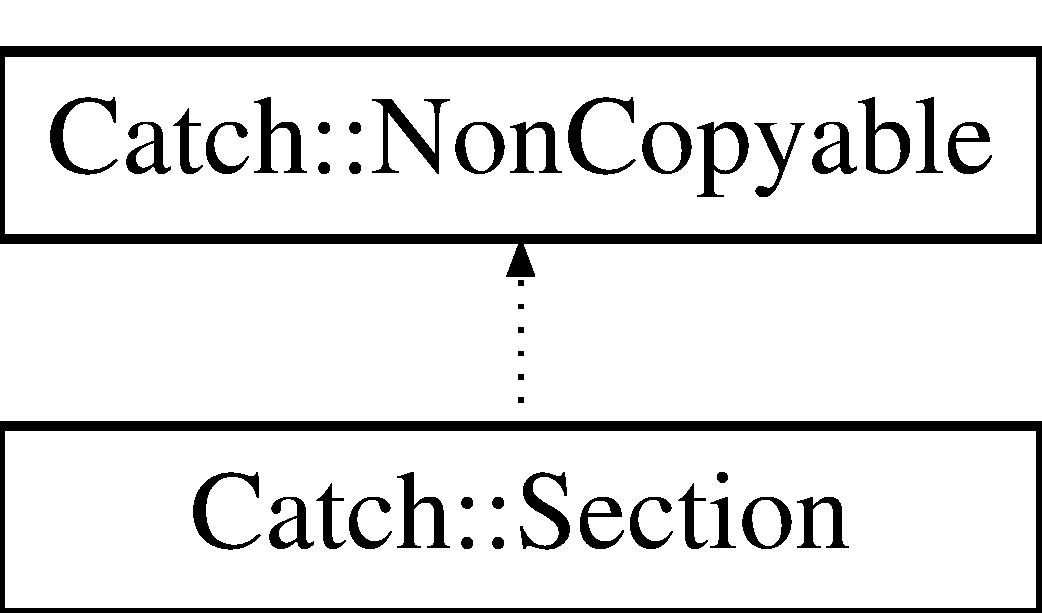
\includegraphics[height=2.000000cm]{class_catch_1_1_section}
\end{center}
\end{figure}
\subsection*{Public Member Functions}
\begin{DoxyCompactItemize}
\item 
\mbox{\hyperlink{class_catch_1_1_section_a68fd4e51e8981aaa7ddb00d8a6abd099}{Section}} (\mbox{\hyperlink{struct_catch_1_1_section_info}{Section\+Info}} const \&info)
\item 
\mbox{\hyperlink{class_catch_1_1_section_aa1422edd68a77aa578b5cc6b8b69f86f}{$\sim$\+Section}} ()
\item 
\mbox{\hyperlink{class_catch_1_1_section_a0632b804dcea1417a2970620a9742eb3}{operator bool}} () const
\end{DoxyCompactItemize}


\subsection{Detailed Description}


Definition at line 1827 of file catch.\+hpp.



\subsection{Constructor \& Destructor Documentation}
\mbox{\Hypertarget{class_catch_1_1_section_a68fd4e51e8981aaa7ddb00d8a6abd099}\label{class_catch_1_1_section_a68fd4e51e8981aaa7ddb00d8a6abd099}} 
\index{Catch\+::\+Section@{Catch\+::\+Section}!Section@{Section}}
\index{Section@{Section}!Catch\+::\+Section@{Catch\+::\+Section}}
\subsubsection{\texorpdfstring{Section()}{Section()}}
{\footnotesize\ttfamily Catch\+::\+Section\+::\+Section (\begin{DoxyParamCaption}\item[{\mbox{\hyperlink{struct_catch_1_1_section_info}{Section\+Info}} const \&}]{info }\end{DoxyParamCaption})}

\mbox{\Hypertarget{class_catch_1_1_section_aa1422edd68a77aa578b5cc6b8b69f86f}\label{class_catch_1_1_section_aa1422edd68a77aa578b5cc6b8b69f86f}} 
\index{Catch\+::\+Section@{Catch\+::\+Section}!````~Section@{$\sim$\+Section}}
\index{````~Section@{$\sim$\+Section}!Catch\+::\+Section@{Catch\+::\+Section}}
\subsubsection{\texorpdfstring{$\sim$\+Section()}{~Section()}}
{\footnotesize\ttfamily Catch\+::\+Section\+::$\sim$\+Section (\begin{DoxyParamCaption}{ }\end{DoxyParamCaption})}



\subsection{Member Function Documentation}
\mbox{\Hypertarget{class_catch_1_1_section_a0632b804dcea1417a2970620a9742eb3}\label{class_catch_1_1_section_a0632b804dcea1417a2970620a9742eb3}} 
\index{Catch\+::\+Section@{Catch\+::\+Section}!operator bool@{operator bool}}
\index{operator bool@{operator bool}!Catch\+::\+Section@{Catch\+::\+Section}}
\subsubsection{\texorpdfstring{operator bool()}{operator bool()}}
{\footnotesize\ttfamily Catch\+::\+Section\+::operator bool (\begin{DoxyParamCaption}{ }\end{DoxyParamCaption}) const\hspace{0.3cm}{\ttfamily [explicit]}}



The documentation for this class was generated from the following file\+:\begin{DoxyCompactItemize}
\item 
D\+:/c++/block\+\_\+matrix-\/master/block\+\_\+matrix-\/master/test/\mbox{\hyperlink{catch_8hpp}{catch.\+hpp}}\end{DoxyCompactItemize}

\hypertarget{struct_catch_1_1_section_end_info}{}\section{Catch\+:\+:Section\+End\+Info Struct Reference}
\label{struct_catch_1_1_section_end_info}\index{Catch\+::\+Section\+End\+Info@{Catch\+::\+Section\+End\+Info}}


{\ttfamily \#include $<$catch.\+hpp$>$}

\subsection*{Public Member Functions}
\begin{DoxyCompactItemize}
\item 
\mbox{\hyperlink{struct_catch_1_1_section_end_info_abc9381c7c22b6907317ec985ccaa6713}{Section\+End\+Info}} (\mbox{\hyperlink{struct_catch_1_1_section_info}{Section\+Info}} const \&\+\_\+section\+Info, \mbox{\hyperlink{struct_catch_1_1_counts}{Counts}} const \&\+\_\+prev\+Assertions, double \+\_\+duration\+In\+Seconds)
\end{DoxyCompactItemize}
\subsection*{Public Attributes}
\begin{DoxyCompactItemize}
\item 
\mbox{\hyperlink{struct_catch_1_1_section_info}{Section\+Info}} \mbox{\hyperlink{struct_catch_1_1_section_end_info_a2d44793392cb83735d086d726822abe9}{section\+Info}}
\item 
\mbox{\hyperlink{struct_catch_1_1_counts}{Counts}} \mbox{\hyperlink{struct_catch_1_1_section_end_info_ae70b154cbc05b5dd2901d97f89303d8c}{prev\+Assertions}}
\item 
double \mbox{\hyperlink{struct_catch_1_1_section_end_info_a7c262f2dab9cff166b8eca620c47eea5}{duration\+In\+Seconds}}
\end{DoxyCompactItemize}


\subsection{Detailed Description}


Definition at line 1790 of file catch.\+hpp.



\subsection{Constructor \& Destructor Documentation}
\mbox{\Hypertarget{struct_catch_1_1_section_end_info_abc9381c7c22b6907317ec985ccaa6713}\label{struct_catch_1_1_section_end_info_abc9381c7c22b6907317ec985ccaa6713}} 
\index{Catch\+::\+Section\+End\+Info@{Catch\+::\+Section\+End\+Info}!Section\+End\+Info@{Section\+End\+Info}}
\index{Section\+End\+Info@{Section\+End\+Info}!Catch\+::\+Section\+End\+Info@{Catch\+::\+Section\+End\+Info}}
\subsubsection{\texorpdfstring{Section\+End\+Info()}{SectionEndInfo()}}
{\footnotesize\ttfamily Catch\+::\+Section\+End\+Info\+::\+Section\+End\+Info (\begin{DoxyParamCaption}\item[{\mbox{\hyperlink{struct_catch_1_1_section_info}{Section\+Info}} const \&}]{\+\_\+section\+Info,  }\item[{\mbox{\hyperlink{struct_catch_1_1_counts}{Counts}} const \&}]{\+\_\+prev\+Assertions,  }\item[{double}]{\+\_\+duration\+In\+Seconds }\end{DoxyParamCaption})}



\subsection{Member Data Documentation}
\mbox{\Hypertarget{struct_catch_1_1_section_end_info_a7c262f2dab9cff166b8eca620c47eea5}\label{struct_catch_1_1_section_end_info_a7c262f2dab9cff166b8eca620c47eea5}} 
\index{Catch\+::\+Section\+End\+Info@{Catch\+::\+Section\+End\+Info}!duration\+In\+Seconds@{duration\+In\+Seconds}}
\index{duration\+In\+Seconds@{duration\+In\+Seconds}!Catch\+::\+Section\+End\+Info@{Catch\+::\+Section\+End\+Info}}
\subsubsection{\texorpdfstring{duration\+In\+Seconds}{durationInSeconds}}
{\footnotesize\ttfamily double Catch\+::\+Section\+End\+Info\+::duration\+In\+Seconds}



Definition at line 1795 of file catch.\+hpp.

\mbox{\Hypertarget{struct_catch_1_1_section_end_info_ae70b154cbc05b5dd2901d97f89303d8c}\label{struct_catch_1_1_section_end_info_ae70b154cbc05b5dd2901d97f89303d8c}} 
\index{Catch\+::\+Section\+End\+Info@{Catch\+::\+Section\+End\+Info}!prev\+Assertions@{prev\+Assertions}}
\index{prev\+Assertions@{prev\+Assertions}!Catch\+::\+Section\+End\+Info@{Catch\+::\+Section\+End\+Info}}
\subsubsection{\texorpdfstring{prev\+Assertions}{prevAssertions}}
{\footnotesize\ttfamily \mbox{\hyperlink{struct_catch_1_1_counts}{Counts}} Catch\+::\+Section\+End\+Info\+::prev\+Assertions}



Definition at line 1794 of file catch.\+hpp.

\mbox{\Hypertarget{struct_catch_1_1_section_end_info_a2d44793392cb83735d086d726822abe9}\label{struct_catch_1_1_section_end_info_a2d44793392cb83735d086d726822abe9}} 
\index{Catch\+::\+Section\+End\+Info@{Catch\+::\+Section\+End\+Info}!section\+Info@{section\+Info}}
\index{section\+Info@{section\+Info}!Catch\+::\+Section\+End\+Info@{Catch\+::\+Section\+End\+Info}}
\subsubsection{\texorpdfstring{section\+Info}{sectionInfo}}
{\footnotesize\ttfamily \mbox{\hyperlink{struct_catch_1_1_section_info}{Section\+Info}} Catch\+::\+Section\+End\+Info\+::section\+Info}



Definition at line 1793 of file catch.\+hpp.



The documentation for this struct was generated from the following file\+:\begin{DoxyCompactItemize}
\item 
D\+:/c++/block\+\_\+matrix-\/master/block\+\_\+matrix-\/master/test/\mbox{\hyperlink{catch_8hpp}{catch.\+hpp}}\end{DoxyCompactItemize}

\hypertarget{struct_catch_1_1_section_info}{}\section{Catch\+:\+:Section\+Info Struct Reference}
\label{struct_catch_1_1_section_info}\index{Catch\+::\+Section\+Info@{Catch\+::\+Section\+Info}}


{\ttfamily \#include $<$catch.\+hpp$>$}

\subsection*{Public Member Functions}
\begin{DoxyCompactItemize}
\item 
\mbox{\hyperlink{struct_catch_1_1_section_info_a27aff3aaf8b6611f3651b17111a272c6}{Section\+Info}} (\mbox{\hyperlink{struct_catch_1_1_source_line_info}{Source\+Line\+Info}} const \&\+\_\+line\+Info, std\+::string const \&\+\_\+name, std\+::string const \&\+\_\+description=std\+::string())
\end{DoxyCompactItemize}
\subsection*{Public Attributes}
\begin{DoxyCompactItemize}
\item 
std\+::string \mbox{\hyperlink{struct_catch_1_1_section_info_a704c8fc662d309137e0d4f199cb7df58}{name}}
\item 
std\+::string \mbox{\hyperlink{struct_catch_1_1_section_info_a0052060219a6de74bb7ade34d4163a4e}{description}}
\item 
\mbox{\hyperlink{struct_catch_1_1_source_line_info}{Source\+Line\+Info}} \mbox{\hyperlink{struct_catch_1_1_section_info_adbc83b8a3507c4acc8ee249e93465711}{line\+Info}}
\end{DoxyCompactItemize}


\subsection{Detailed Description}


Definition at line 1779 of file catch.\+hpp.



\subsection{Constructor \& Destructor Documentation}
\mbox{\Hypertarget{struct_catch_1_1_section_info_a27aff3aaf8b6611f3651b17111a272c6}\label{struct_catch_1_1_section_info_a27aff3aaf8b6611f3651b17111a272c6}} 
\index{Catch\+::\+Section\+Info@{Catch\+::\+Section\+Info}!Section\+Info@{Section\+Info}}
\index{Section\+Info@{Section\+Info}!Catch\+::\+Section\+Info@{Catch\+::\+Section\+Info}}
\subsubsection{\texorpdfstring{Section\+Info()}{SectionInfo()}}
{\footnotesize\ttfamily Catch\+::\+Section\+Info\+::\+Section\+Info (\begin{DoxyParamCaption}\item[{\mbox{\hyperlink{struct_catch_1_1_source_line_info}{Source\+Line\+Info}} const \&}]{\+\_\+line\+Info,  }\item[{std\+::string const \&}]{\+\_\+name,  }\item[{std\+::string const \&}]{\+\_\+description = {\ttfamily std\+:\+:string()} }\end{DoxyParamCaption})}



\subsection{Member Data Documentation}
\mbox{\Hypertarget{struct_catch_1_1_section_info_a0052060219a6de74bb7ade34d4163a4e}\label{struct_catch_1_1_section_info_a0052060219a6de74bb7ade34d4163a4e}} 
\index{Catch\+::\+Section\+Info@{Catch\+::\+Section\+Info}!description@{description}}
\index{description@{description}!Catch\+::\+Section\+Info@{Catch\+::\+Section\+Info}}
\subsubsection{\texorpdfstring{description}{description}}
{\footnotesize\ttfamily std\+::string Catch\+::\+Section\+Info\+::description}



Definition at line 1786 of file catch.\+hpp.

\mbox{\Hypertarget{struct_catch_1_1_section_info_adbc83b8a3507c4acc8ee249e93465711}\label{struct_catch_1_1_section_info_adbc83b8a3507c4acc8ee249e93465711}} 
\index{Catch\+::\+Section\+Info@{Catch\+::\+Section\+Info}!line\+Info@{line\+Info}}
\index{line\+Info@{line\+Info}!Catch\+::\+Section\+Info@{Catch\+::\+Section\+Info}}
\subsubsection{\texorpdfstring{line\+Info}{lineInfo}}
{\footnotesize\ttfamily \mbox{\hyperlink{struct_catch_1_1_source_line_info}{Source\+Line\+Info}} Catch\+::\+Section\+Info\+::line\+Info}



Definition at line 1787 of file catch.\+hpp.

\mbox{\Hypertarget{struct_catch_1_1_section_info_a704c8fc662d309137e0d4f199cb7df58}\label{struct_catch_1_1_section_info_a704c8fc662d309137e0d4f199cb7df58}} 
\index{Catch\+::\+Section\+Info@{Catch\+::\+Section\+Info}!name@{name}}
\index{name@{name}!Catch\+::\+Section\+Info@{Catch\+::\+Section\+Info}}
\subsubsection{\texorpdfstring{name}{name}}
{\footnotesize\ttfamily std\+::string Catch\+::\+Section\+Info\+::name}



Definition at line 1785 of file catch.\+hpp.



The documentation for this struct was generated from the following file\+:\begin{DoxyCompactItemize}
\item 
D\+:/c++/block\+\_\+matrix-\/master/block\+\_\+matrix-\/master/test/\mbox{\hyperlink{catch_8hpp}{catch.\+hpp}}\end{DoxyCompactItemize}

\hypertarget{struct_catch_1_1_source_line_info}{}\section{Catch\+:\+:Source\+Line\+Info Struct Reference}
\label{struct_catch_1_1_source_line_info}\index{Catch\+::\+Source\+Line\+Info@{Catch\+::\+Source\+Line\+Info}}


{\ttfamily \#include $<$catch.\+hpp$>$}

\subsection*{Public Member Functions}
\begin{DoxyCompactItemize}
\item 
\mbox{\hyperlink{struct_catch_1_1_source_line_info_a2d80932bb4129b1606d1924a5c44be2f}{Source\+Line\+Info}} ()=delete
\item 
\mbox{\hyperlink{struct_catch_1_1_source_line_info_a48510b82a39a042ab370ed143dd30c10}{Source\+Line\+Info}} (char const $\ast$\+\_\+file, std\+::size\+\_\+t \+\_\+line) noexcept
\item 
\mbox{\hyperlink{struct_catch_1_1_source_line_info_a7c44c9986c33a9cf842b791374332d41}{Source\+Line\+Info}} (\mbox{\hyperlink{struct_catch_1_1_source_line_info}{Source\+Line\+Info}} const \&other)=default
\item 
\mbox{\hyperlink{struct_catch_1_1_source_line_info_a6614b503b493bbdd3b49a1bd732e0a55}{Source\+Line\+Info}} (\mbox{\hyperlink{struct_catch_1_1_source_line_info}{Source\+Line\+Info}} \&\&)=default
\item 
\mbox{\hyperlink{struct_catch_1_1_source_line_info}{Source\+Line\+Info}} \& \mbox{\hyperlink{struct_catch_1_1_source_line_info_a1a6cfc0197357ef4e329bb256aa8a354}{operator=}} (\mbox{\hyperlink{struct_catch_1_1_source_line_info}{Source\+Line\+Info}} const \&)=default
\item 
\mbox{\hyperlink{struct_catch_1_1_source_line_info}{Source\+Line\+Info}} \& \mbox{\hyperlink{struct_catch_1_1_source_line_info_a7fa35372f2bca5e91adc25327b7c753c}{operator=}} (\mbox{\hyperlink{struct_catch_1_1_source_line_info}{Source\+Line\+Info}} \&\&)=default
\item 
bool \mbox{\hyperlink{struct_catch_1_1_source_line_info_a10a5b5b7dff82971879c2eb8d83f9b3b}{empty}} () const noexcept
\item 
bool \mbox{\hyperlink{struct_catch_1_1_source_line_info_af07e4fdeddf8409b91e4f842f6264cf8}{operator==}} (\mbox{\hyperlink{struct_catch_1_1_source_line_info}{Source\+Line\+Info}} const \&other) const noexcept
\item 
bool \mbox{\hyperlink{struct_catch_1_1_source_line_info_af77415416919d2d6030b4be085b92f7a}{operator$<$}} (\mbox{\hyperlink{struct_catch_1_1_source_line_info}{Source\+Line\+Info}} const \&other) const noexcept
\end{DoxyCompactItemize}
\subsection*{Public Attributes}
\begin{DoxyCompactItemize}
\item 
char const  $\ast$ \mbox{\hyperlink{struct_catch_1_1_source_line_info_ad65537703e9f08c1fa7777fbc3f0c617}{file}}
\item 
std\+::size\+\_\+t \mbox{\hyperlink{struct_catch_1_1_source_line_info_a841e5d696c7b9cde24e45e61dd979c77}{line}}
\end{DoxyCompactItemize}


\subsection{Detailed Description}


Definition at line 272 of file catch.\+hpp.



\subsection{Constructor \& Destructor Documentation}
\mbox{\Hypertarget{struct_catch_1_1_source_line_info_a2d80932bb4129b1606d1924a5c44be2f}\label{struct_catch_1_1_source_line_info_a2d80932bb4129b1606d1924a5c44be2f}} 
\index{Catch\+::\+Source\+Line\+Info@{Catch\+::\+Source\+Line\+Info}!Source\+Line\+Info@{Source\+Line\+Info}}
\index{Source\+Line\+Info@{Source\+Line\+Info}!Catch\+::\+Source\+Line\+Info@{Catch\+::\+Source\+Line\+Info}}
\subsubsection{\texorpdfstring{Source\+Line\+Info()}{SourceLineInfo()}\hspace{0.1cm}{\footnotesize\ttfamily [1/4]}}
{\footnotesize\ttfamily Catch\+::\+Source\+Line\+Info\+::\+Source\+Line\+Info (\begin{DoxyParamCaption}{ }\end{DoxyParamCaption})\hspace{0.3cm}{\ttfamily [delete]}}

\mbox{\Hypertarget{struct_catch_1_1_source_line_info_a48510b82a39a042ab370ed143dd30c10}\label{struct_catch_1_1_source_line_info_a48510b82a39a042ab370ed143dd30c10}} 
\index{Catch\+::\+Source\+Line\+Info@{Catch\+::\+Source\+Line\+Info}!Source\+Line\+Info@{Source\+Line\+Info}}
\index{Source\+Line\+Info@{Source\+Line\+Info}!Catch\+::\+Source\+Line\+Info@{Catch\+::\+Source\+Line\+Info}}
\subsubsection{\texorpdfstring{Source\+Line\+Info()}{SourceLineInfo()}\hspace{0.1cm}{\footnotesize\ttfamily [2/4]}}
{\footnotesize\ttfamily Catch\+::\+Source\+Line\+Info\+::\+Source\+Line\+Info (\begin{DoxyParamCaption}\item[{char const $\ast$}]{\+\_\+file,  }\item[{std\+::size\+\_\+t}]{\+\_\+line }\end{DoxyParamCaption})\hspace{0.3cm}{\ttfamily [inline]}, {\ttfamily [noexcept]}}



Definition at line 275 of file catch.\+hpp.

\mbox{\Hypertarget{struct_catch_1_1_source_line_info_a7c44c9986c33a9cf842b791374332d41}\label{struct_catch_1_1_source_line_info_a7c44c9986c33a9cf842b791374332d41}} 
\index{Catch\+::\+Source\+Line\+Info@{Catch\+::\+Source\+Line\+Info}!Source\+Line\+Info@{Source\+Line\+Info}}
\index{Source\+Line\+Info@{Source\+Line\+Info}!Catch\+::\+Source\+Line\+Info@{Catch\+::\+Source\+Line\+Info}}
\subsubsection{\texorpdfstring{Source\+Line\+Info()}{SourceLineInfo()}\hspace{0.1cm}{\footnotesize\ttfamily [3/4]}}
{\footnotesize\ttfamily Catch\+::\+Source\+Line\+Info\+::\+Source\+Line\+Info (\begin{DoxyParamCaption}\item[{\mbox{\hyperlink{struct_catch_1_1_source_line_info}{Source\+Line\+Info}} const \&}]{other }\end{DoxyParamCaption})\hspace{0.3cm}{\ttfamily [default]}}

\mbox{\Hypertarget{struct_catch_1_1_source_line_info_a6614b503b493bbdd3b49a1bd732e0a55}\label{struct_catch_1_1_source_line_info_a6614b503b493bbdd3b49a1bd732e0a55}} 
\index{Catch\+::\+Source\+Line\+Info@{Catch\+::\+Source\+Line\+Info}!Source\+Line\+Info@{Source\+Line\+Info}}
\index{Source\+Line\+Info@{Source\+Line\+Info}!Catch\+::\+Source\+Line\+Info@{Catch\+::\+Source\+Line\+Info}}
\subsubsection{\texorpdfstring{Source\+Line\+Info()}{SourceLineInfo()}\hspace{0.1cm}{\footnotesize\ttfamily [4/4]}}
{\footnotesize\ttfamily Catch\+::\+Source\+Line\+Info\+::\+Source\+Line\+Info (\begin{DoxyParamCaption}\item[{\mbox{\hyperlink{struct_catch_1_1_source_line_info}{Source\+Line\+Info}} \&\&}]{ }\end{DoxyParamCaption})\hspace{0.3cm}{\ttfamily [default]}}



\subsection{Member Function Documentation}
\mbox{\Hypertarget{struct_catch_1_1_source_line_info_a10a5b5b7dff82971879c2eb8d83f9b3b}\label{struct_catch_1_1_source_line_info_a10a5b5b7dff82971879c2eb8d83f9b3b}} 
\index{Catch\+::\+Source\+Line\+Info@{Catch\+::\+Source\+Line\+Info}!empty@{empty}}
\index{empty@{empty}!Catch\+::\+Source\+Line\+Info@{Catch\+::\+Source\+Line\+Info}}
\subsubsection{\texorpdfstring{empty()}{empty()}}
{\footnotesize\ttfamily bool Catch\+::\+Source\+Line\+Info\+::empty (\begin{DoxyParamCaption}{ }\end{DoxyParamCaption}) const\hspace{0.3cm}{\ttfamily [noexcept]}}

\mbox{\Hypertarget{struct_catch_1_1_source_line_info_af77415416919d2d6030b4be085b92f7a}\label{struct_catch_1_1_source_line_info_af77415416919d2d6030b4be085b92f7a}} 
\index{Catch\+::\+Source\+Line\+Info@{Catch\+::\+Source\+Line\+Info}!operator$<$@{operator$<$}}
\index{operator$<$@{operator$<$}!Catch\+::\+Source\+Line\+Info@{Catch\+::\+Source\+Line\+Info}}
\subsubsection{\texorpdfstring{operator$<$()}{operator<()}}
{\footnotesize\ttfamily bool Catch\+::\+Source\+Line\+Info\+::operator$<$ (\begin{DoxyParamCaption}\item[{\mbox{\hyperlink{struct_catch_1_1_source_line_info}{Source\+Line\+Info}} const \&}]{other }\end{DoxyParamCaption}) const\hspace{0.3cm}{\ttfamily [noexcept]}}

\mbox{\Hypertarget{struct_catch_1_1_source_line_info_a1a6cfc0197357ef4e329bb256aa8a354}\label{struct_catch_1_1_source_line_info_a1a6cfc0197357ef4e329bb256aa8a354}} 
\index{Catch\+::\+Source\+Line\+Info@{Catch\+::\+Source\+Line\+Info}!operator=@{operator=}}
\index{operator=@{operator=}!Catch\+::\+Source\+Line\+Info@{Catch\+::\+Source\+Line\+Info}}
\subsubsection{\texorpdfstring{operator=()}{operator=()}\hspace{0.1cm}{\footnotesize\ttfamily [1/2]}}
{\footnotesize\ttfamily \mbox{\hyperlink{struct_catch_1_1_source_line_info}{Source\+Line\+Info}}\& Catch\+::\+Source\+Line\+Info\+::operator= (\begin{DoxyParamCaption}\item[{\mbox{\hyperlink{struct_catch_1_1_source_line_info}{Source\+Line\+Info}} const \&}]{ }\end{DoxyParamCaption})\hspace{0.3cm}{\ttfamily [default]}}

\mbox{\Hypertarget{struct_catch_1_1_source_line_info_a7fa35372f2bca5e91adc25327b7c753c}\label{struct_catch_1_1_source_line_info_a7fa35372f2bca5e91adc25327b7c753c}} 
\index{Catch\+::\+Source\+Line\+Info@{Catch\+::\+Source\+Line\+Info}!operator=@{operator=}}
\index{operator=@{operator=}!Catch\+::\+Source\+Line\+Info@{Catch\+::\+Source\+Line\+Info}}
\subsubsection{\texorpdfstring{operator=()}{operator=()}\hspace{0.1cm}{\footnotesize\ttfamily [2/2]}}
{\footnotesize\ttfamily \mbox{\hyperlink{struct_catch_1_1_source_line_info}{Source\+Line\+Info}}\& Catch\+::\+Source\+Line\+Info\+::operator= (\begin{DoxyParamCaption}\item[{\mbox{\hyperlink{struct_catch_1_1_source_line_info}{Source\+Line\+Info}} \&\&}]{ }\end{DoxyParamCaption})\hspace{0.3cm}{\ttfamily [default]}}

\mbox{\Hypertarget{struct_catch_1_1_source_line_info_af07e4fdeddf8409b91e4f842f6264cf8}\label{struct_catch_1_1_source_line_info_af07e4fdeddf8409b91e4f842f6264cf8}} 
\index{Catch\+::\+Source\+Line\+Info@{Catch\+::\+Source\+Line\+Info}!operator==@{operator==}}
\index{operator==@{operator==}!Catch\+::\+Source\+Line\+Info@{Catch\+::\+Source\+Line\+Info}}
\subsubsection{\texorpdfstring{operator==()}{operator==()}}
{\footnotesize\ttfamily bool Catch\+::\+Source\+Line\+Info\+::operator== (\begin{DoxyParamCaption}\item[{\mbox{\hyperlink{struct_catch_1_1_source_line_info}{Source\+Line\+Info}} const \&}]{other }\end{DoxyParamCaption}) const\hspace{0.3cm}{\ttfamily [noexcept]}}



\subsection{Member Data Documentation}
\mbox{\Hypertarget{struct_catch_1_1_source_line_info_ad65537703e9f08c1fa7777fbc3f0c617}\label{struct_catch_1_1_source_line_info_ad65537703e9f08c1fa7777fbc3f0c617}} 
\index{Catch\+::\+Source\+Line\+Info@{Catch\+::\+Source\+Line\+Info}!file@{file}}
\index{file@{file}!Catch\+::\+Source\+Line\+Info@{Catch\+::\+Source\+Line\+Info}}
\subsubsection{\texorpdfstring{file}{file}}
{\footnotesize\ttfamily char const$\ast$ Catch\+::\+Source\+Line\+Info\+::file}



Definition at line 289 of file catch.\+hpp.

\mbox{\Hypertarget{struct_catch_1_1_source_line_info_a841e5d696c7b9cde24e45e61dd979c77}\label{struct_catch_1_1_source_line_info_a841e5d696c7b9cde24e45e61dd979c77}} 
\index{Catch\+::\+Source\+Line\+Info@{Catch\+::\+Source\+Line\+Info}!line@{line}}
\index{line@{line}!Catch\+::\+Source\+Line\+Info@{Catch\+::\+Source\+Line\+Info}}
\subsubsection{\texorpdfstring{line}{line}}
{\footnotesize\ttfamily std\+::size\+\_\+t Catch\+::\+Source\+Line\+Info\+::line}



Definition at line 290 of file catch.\+hpp.



The documentation for this struct was generated from the following file\+:\begin{DoxyCompactItemize}
\item 
D\+:/c++/block\+\_\+matrix-\/master/block\+\_\+matrix-\/master/test/\mbox{\hyperlink{catch_8hpp}{catch.\+hpp}}\end{DoxyCompactItemize}

\hypertarget{struct_catch_1_1_matchers_1_1_std_string_1_1_starts_with_matcher}{}\section{Catch\+:\+:Matchers\+:\+:Std\+String\+:\+:Starts\+With\+Matcher Struct Reference}
\label{struct_catch_1_1_matchers_1_1_std_string_1_1_starts_with_matcher}\index{Catch\+::\+Matchers\+::\+Std\+String\+::\+Starts\+With\+Matcher@{Catch\+::\+Matchers\+::\+Std\+String\+::\+Starts\+With\+Matcher}}


{\ttfamily \#include $<$catch.\+hpp$>$}

Inheritance diagram for Catch\+:\+:Matchers\+:\+:Std\+String\+:\+:Starts\+With\+Matcher\+:\begin{figure}[H]
\begin{center}
\leavevmode
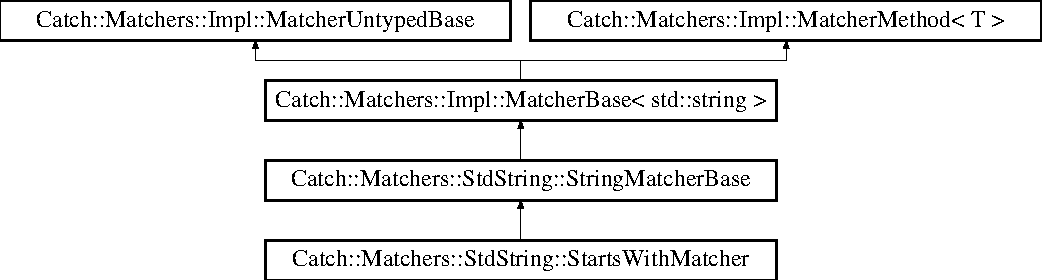
\includegraphics[height=3.758389cm]{struct_catch_1_1_matchers_1_1_std_string_1_1_starts_with_matcher}
\end{center}
\end{figure}
\subsection*{Public Member Functions}
\begin{DoxyCompactItemize}
\item 
\mbox{\hyperlink{struct_catch_1_1_matchers_1_1_std_string_1_1_starts_with_matcher_a7b86f258bdbd131a6e7bcd94a8977325}{Starts\+With\+Matcher}} (\mbox{\hyperlink{struct_catch_1_1_matchers_1_1_std_string_1_1_cased_string}{Cased\+String}} const \&comparator)
\item 
bool \mbox{\hyperlink{struct_catch_1_1_matchers_1_1_std_string_1_1_starts_with_matcher_a7da4747aed0c48989d8be59a89e2b7fb}{match}} (std\+::string const \&source) const override
\end{DoxyCompactItemize}
\subsection*{Additional Inherited Members}


\subsection{Detailed Description}


Definition at line 2395 of file catch.\+hpp.



\subsection{Constructor \& Destructor Documentation}
\mbox{\Hypertarget{struct_catch_1_1_matchers_1_1_std_string_1_1_starts_with_matcher_a7b86f258bdbd131a6e7bcd94a8977325}\label{struct_catch_1_1_matchers_1_1_std_string_1_1_starts_with_matcher_a7b86f258bdbd131a6e7bcd94a8977325}} 
\index{Catch\+::\+Matchers\+::\+Std\+String\+::\+Starts\+With\+Matcher@{Catch\+::\+Matchers\+::\+Std\+String\+::\+Starts\+With\+Matcher}!Starts\+With\+Matcher@{Starts\+With\+Matcher}}
\index{Starts\+With\+Matcher@{Starts\+With\+Matcher}!Catch\+::\+Matchers\+::\+Std\+String\+::\+Starts\+With\+Matcher@{Catch\+::\+Matchers\+::\+Std\+String\+::\+Starts\+With\+Matcher}}
\subsubsection{\texorpdfstring{Starts\+With\+Matcher()}{StartsWithMatcher()}}
{\footnotesize\ttfamily Catch\+::\+Matchers\+::\+Std\+String\+::\+Starts\+With\+Matcher\+::\+Starts\+With\+Matcher (\begin{DoxyParamCaption}\item[{\mbox{\hyperlink{struct_catch_1_1_matchers_1_1_std_string_1_1_cased_string}{Cased\+String}} const \&}]{comparator }\end{DoxyParamCaption})}



\subsection{Member Function Documentation}
\mbox{\Hypertarget{struct_catch_1_1_matchers_1_1_std_string_1_1_starts_with_matcher_a7da4747aed0c48989d8be59a89e2b7fb}\label{struct_catch_1_1_matchers_1_1_std_string_1_1_starts_with_matcher_a7da4747aed0c48989d8be59a89e2b7fb}} 
\index{Catch\+::\+Matchers\+::\+Std\+String\+::\+Starts\+With\+Matcher@{Catch\+::\+Matchers\+::\+Std\+String\+::\+Starts\+With\+Matcher}!match@{match}}
\index{match@{match}!Catch\+::\+Matchers\+::\+Std\+String\+::\+Starts\+With\+Matcher@{Catch\+::\+Matchers\+::\+Std\+String\+::\+Starts\+With\+Matcher}}
\subsubsection{\texorpdfstring{match()}{match()}}
{\footnotesize\ttfamily bool Catch\+::\+Matchers\+::\+Std\+String\+::\+Starts\+With\+Matcher\+::match (\begin{DoxyParamCaption}\item[{std\+::string const \&}]{source }\end{DoxyParamCaption}) const\hspace{0.3cm}{\ttfamily [override]}}



The documentation for this struct was generated from the following file\+:\begin{DoxyCompactItemize}
\item 
D\+:/c++/block\+\_\+matrix-\/master/block\+\_\+matrix-\/master/test/\mbox{\hyperlink{catch_8hpp}{catch.\+hpp}}\end{DoxyCompactItemize}

\hypertarget{struct_catch_1_1_stream_end_stop}{}\section{Catch\+:\+:Stream\+End\+Stop Struct Reference}
\label{struct_catch_1_1_stream_end_stop}\index{Catch\+::\+Stream\+End\+Stop@{Catch\+::\+Stream\+End\+Stop}}


{\ttfamily \#include $<$catch.\+hpp$>$}

\subsection*{Public Member Functions}
\begin{DoxyCompactItemize}
\item 
std\+::string \mbox{\hyperlink{struct_catch_1_1_stream_end_stop_a4a518f0342a381074821d5bda2651401}{operator+}} () const
\end{DoxyCompactItemize}


\subsection{Detailed Description}


Definition at line 299 of file catch.\+hpp.



\subsection{Member Function Documentation}
\mbox{\Hypertarget{struct_catch_1_1_stream_end_stop_a4a518f0342a381074821d5bda2651401}\label{struct_catch_1_1_stream_end_stop_a4a518f0342a381074821d5bda2651401}} 
\index{Catch\+::\+Stream\+End\+Stop@{Catch\+::\+Stream\+End\+Stop}!operator+@{operator+}}
\index{operator+@{operator+}!Catch\+::\+Stream\+End\+Stop@{Catch\+::\+Stream\+End\+Stop}}
\subsubsection{\texorpdfstring{operator+()}{operator+()}}
{\footnotesize\ttfamily std\+::string Catch\+::\+Stream\+End\+Stop\+::operator+ (\begin{DoxyParamCaption}{ }\end{DoxyParamCaption}) const}



The documentation for this struct was generated from the following file\+:\begin{DoxyCompactItemize}
\item 
D\+:/c++/block\+\_\+matrix-\/master/block\+\_\+matrix-\/master/test/\mbox{\hyperlink{catch_8hpp}{catch.\+hpp}}\end{DoxyCompactItemize}

\hypertarget{struct_catch_1_1_string_maker}{}\section{Catch\+:\+:String\+Maker$<$ T, typename $>$ Struct Template Reference}
\label{struct_catch_1_1_string_maker}\index{Catch\+::\+String\+Maker$<$ T, typename $>$@{Catch\+::\+String\+Maker$<$ T, typename $>$}}


{\ttfamily \#include $<$catch.\+hpp$>$}

\subsection*{Static Public Member Functions}
\begin{DoxyCompactItemize}
\item 
{\footnotesize template$<$typename Fake  = T$>$ }\\static std\+::enable\+\_\+if$<$\+::\mbox{\hyperlink{class_catch_1_1_detail_1_1_is_stream_insertable}{Catch\+::\+Detail\+::\+Is\+Stream\+Insertable}}$<$ Fake $>$\+::value, std\+::string $>$\+::type \mbox{\hyperlink{struct_catch_1_1_string_maker_ab2c357e22b754802c4b1351257103eb6}{convert}} (const Fake \&value)
\item 
{\footnotesize template$<$typename Fake  = T$>$ }\\static std\+::enable\+\_\+if$<$!\+::\mbox{\hyperlink{class_catch_1_1_detail_1_1_is_stream_insertable}{Catch\+::\+Detail\+::\+Is\+Stream\+Insertable}}$<$ Fake $>$\+::value, std\+::string $>$\+::type \mbox{\hyperlink{struct_catch_1_1_string_maker_a68bb548de0e5ad364228b1ca3dd2f561}{convert}} (const Fake \&value)
\end{DoxyCompactItemize}


\subsection{Detailed Description}
\subsubsection*{template$<$typename T, typename = void$>$\newline
struct Catch\+::\+String\+Maker$<$ T, typename $>$}



Definition at line 790 of file catch.\+hpp.



\subsection{Member Function Documentation}
\mbox{\Hypertarget{struct_catch_1_1_string_maker_ab2c357e22b754802c4b1351257103eb6}\label{struct_catch_1_1_string_maker_ab2c357e22b754802c4b1351257103eb6}} 
\index{Catch\+::\+String\+Maker@{Catch\+::\+String\+Maker}!convert@{convert}}
\index{convert@{convert}!Catch\+::\+String\+Maker@{Catch\+::\+String\+Maker}}
\subsubsection{\texorpdfstring{convert()}{convert()}\hspace{0.1cm}{\footnotesize\ttfamily [1/2]}}
{\footnotesize\ttfamily template$<$typename T , typename  = void$>$ \\
template$<$typename Fake  = T$>$ \\
static std\+::enable\+\_\+if$<$\+::\mbox{\hyperlink{class_catch_1_1_detail_1_1_is_stream_insertable}{Catch\+::\+Detail\+::\+Is\+Stream\+Insertable}}$<$Fake$>$\+::value, std\+::string$>$\+::type \mbox{\hyperlink{struct_catch_1_1_string_maker}{Catch\+::\+String\+Maker}}$<$ T, typename $>$\+::convert (\begin{DoxyParamCaption}\item[{const Fake \&}]{value }\end{DoxyParamCaption})\hspace{0.3cm}{\ttfamily [inline]}, {\ttfamily [static]}}



Definition at line 794 of file catch.\+hpp.

\mbox{\Hypertarget{struct_catch_1_1_string_maker_a68bb548de0e5ad364228b1ca3dd2f561}\label{struct_catch_1_1_string_maker_a68bb548de0e5ad364228b1ca3dd2f561}} 
\index{Catch\+::\+String\+Maker@{Catch\+::\+String\+Maker}!convert@{convert}}
\index{convert@{convert}!Catch\+::\+String\+Maker@{Catch\+::\+String\+Maker}}
\subsubsection{\texorpdfstring{convert()}{convert()}\hspace{0.1cm}{\footnotesize\ttfamily [2/2]}}
{\footnotesize\ttfamily template$<$typename T , typename  = void$>$ \\
template$<$typename Fake  = T$>$ \\
static std\+::enable\+\_\+if$<$!\+::\mbox{\hyperlink{class_catch_1_1_detail_1_1_is_stream_insertable}{Catch\+::\+Detail\+::\+Is\+Stream\+Insertable}}$<$Fake$>$\+::value, std\+::string$>$\+::type \mbox{\hyperlink{struct_catch_1_1_string_maker}{Catch\+::\+String\+Maker}}$<$ T, typename $>$\+::convert (\begin{DoxyParamCaption}\item[{const Fake \&}]{value }\end{DoxyParamCaption})\hspace{0.3cm}{\ttfamily [inline]}, {\ttfamily [static]}}



Definition at line 803 of file catch.\+hpp.



The documentation for this struct was generated from the following file\+:\begin{DoxyCompactItemize}
\item 
D\+:/c++/block\+\_\+matrix-\/master/block\+\_\+matrix-\/master/test/\mbox{\hyperlink{catch_8hpp}{catch.\+hpp}}\end{DoxyCompactItemize}

\hypertarget{struct_catch_1_1_string_maker_3_01bool_01_4}{}\section{Catch\+:\+:String\+Maker$<$ bool $>$ Struct Template Reference}
\label{struct_catch_1_1_string_maker_3_01bool_01_4}\index{Catch\+::\+String\+Maker$<$ bool $>$@{Catch\+::\+String\+Maker$<$ bool $>$}}


{\ttfamily \#include $<$catch.\+hpp$>$}

\subsection*{Static Public Member Functions}
\begin{DoxyCompactItemize}
\item 
static std\+::string \mbox{\hyperlink{struct_catch_1_1_string_maker_3_01bool_01_4_a37e9899c82c4b4515f876f16f8957a77}{convert}} (bool b)
\end{DoxyCompactItemize}


\subsection{Detailed Description}
\subsubsection*{template$<$$>$\newline
struct Catch\+::\+String\+Maker$<$ bool $>$}



Definition at line 901 of file catch.\+hpp.



\subsection{Member Function Documentation}
\mbox{\Hypertarget{struct_catch_1_1_string_maker_3_01bool_01_4_a37e9899c82c4b4515f876f16f8957a77}\label{struct_catch_1_1_string_maker_3_01bool_01_4_a37e9899c82c4b4515f876f16f8957a77}} 
\index{Catch\+::\+String\+Maker$<$ bool $>$@{Catch\+::\+String\+Maker$<$ bool $>$}!convert@{convert}}
\index{convert@{convert}!Catch\+::\+String\+Maker$<$ bool $>$@{Catch\+::\+String\+Maker$<$ bool $>$}}
\subsubsection{\texorpdfstring{convert()}{convert()}}
{\footnotesize\ttfamily static std\+::string \mbox{\hyperlink{struct_catch_1_1_string_maker}{Catch\+::\+String\+Maker}}$<$ bool $>$\+::convert (\begin{DoxyParamCaption}\item[{bool}]{b }\end{DoxyParamCaption})\hspace{0.3cm}{\ttfamily [static]}}



The documentation for this struct was generated from the following file\+:\begin{DoxyCompactItemize}
\item 
D\+:/c++/block\+\_\+matrix-\/master/block\+\_\+matrix-\/master/test/\mbox{\hyperlink{catch_8hpp}{catch.\+hpp}}\end{DoxyCompactItemize}

\hypertarget{struct_catch_1_1_string_maker_3_01_catch_1_1_detail_1_1_approx_01_4}{}\section{Catch\+:\+:String\+Maker$<$ Catch\+:\+:Detail\+:\+:Approx $>$ Struct Template Reference}
\label{struct_catch_1_1_string_maker_3_01_catch_1_1_detail_1_1_approx_01_4}\index{Catch\+::\+String\+Maker$<$ Catch\+::\+Detail\+::\+Approx $>$@{Catch\+::\+String\+Maker$<$ Catch\+::\+Detail\+::\+Approx $>$}}


{\ttfamily \#include $<$catch.\+hpp$>$}

\subsection*{Static Public Member Functions}
\begin{DoxyCompactItemize}
\item 
static std\+::string \mbox{\hyperlink{struct_catch_1_1_string_maker_3_01_catch_1_1_detail_1_1_approx_01_4_a8e5015720682fecfbff0f05de19a698f}{convert}} (\mbox{\hyperlink{class_catch_1_1_detail_1_1_approx}{Catch\+::\+Detail\+::\+Approx}} const \&value)
\end{DoxyCompactItemize}


\subsection{Detailed Description}
\subsubsection*{template$<$$>$\newline
struct Catch\+::\+String\+Maker$<$ Catch\+::\+Detail\+::\+Approx $>$}



Definition at line 2132 of file catch.\+hpp.



\subsection{Member Function Documentation}
\mbox{\Hypertarget{struct_catch_1_1_string_maker_3_01_catch_1_1_detail_1_1_approx_01_4_a8e5015720682fecfbff0f05de19a698f}\label{struct_catch_1_1_string_maker_3_01_catch_1_1_detail_1_1_approx_01_4_a8e5015720682fecfbff0f05de19a698f}} 
\index{Catch\+::\+String\+Maker$<$ Catch\+::\+Detail\+::\+Approx $>$@{Catch\+::\+String\+Maker$<$ Catch\+::\+Detail\+::\+Approx $>$}!convert@{convert}}
\index{convert@{convert}!Catch\+::\+String\+Maker$<$ Catch\+::\+Detail\+::\+Approx $>$@{Catch\+::\+String\+Maker$<$ Catch\+::\+Detail\+::\+Approx $>$}}
\subsubsection{\texorpdfstring{convert()}{convert()}}
{\footnotesize\ttfamily static std\+::string \mbox{\hyperlink{struct_catch_1_1_string_maker}{Catch\+::\+String\+Maker}}$<$ \mbox{\hyperlink{class_catch_1_1_detail_1_1_approx}{Catch\+::\+Detail\+::\+Approx}} $>$\+::convert (\begin{DoxyParamCaption}\item[{\mbox{\hyperlink{class_catch_1_1_detail_1_1_approx}{Catch\+::\+Detail\+::\+Approx}} const \&}]{value }\end{DoxyParamCaption})\hspace{0.3cm}{\ttfamily [static]}}



The documentation for this struct was generated from the following file\+:\begin{DoxyCompactItemize}
\item 
D\+:/c++/block\+\_\+matrix-\/master/block\+\_\+matrix-\/master/test/\mbox{\hyperlink{catch_8hpp}{catch.\+hpp}}\end{DoxyCompactItemize}

\hypertarget{struct_catch_1_1_string_maker_3_01char_01_5_01_4}{}\section{Catch\+:\+:String\+Maker$<$ char $\ast$ $>$ Struct Template Reference}
\label{struct_catch_1_1_string_maker_3_01char_01_5_01_4}\index{Catch\+::\+String\+Maker$<$ char $\ast$ $>$@{Catch\+::\+String\+Maker$<$ char $\ast$ $>$}}


{\ttfamily \#include $<$catch.\+hpp$>$}

\subsection*{Static Public Member Functions}
\begin{DoxyCompactItemize}
\item 
static std\+::string \mbox{\hyperlink{struct_catch_1_1_string_maker_3_01char_01_5_01_4_a33049e24281ea6fba48bd8817bdd52bd}{convert}} (char $\ast$str)
\end{DoxyCompactItemize}


\subsection{Detailed Description}
\subsubsection*{template$<$$>$\newline
struct Catch\+::\+String\+Maker$<$ char $\ast$ $>$}



Definition at line 842 of file catch.\+hpp.



\subsection{Member Function Documentation}
\mbox{\Hypertarget{struct_catch_1_1_string_maker_3_01char_01_5_01_4_a33049e24281ea6fba48bd8817bdd52bd}\label{struct_catch_1_1_string_maker_3_01char_01_5_01_4_a33049e24281ea6fba48bd8817bdd52bd}} 
\index{Catch\+::\+String\+Maker$<$ char $\ast$ $>$@{Catch\+::\+String\+Maker$<$ char $\ast$ $>$}!convert@{convert}}
\index{convert@{convert}!Catch\+::\+String\+Maker$<$ char $\ast$ $>$@{Catch\+::\+String\+Maker$<$ char $\ast$ $>$}}
\subsubsection{\texorpdfstring{convert()}{convert()}}
{\footnotesize\ttfamily static std\+::string \mbox{\hyperlink{struct_catch_1_1_string_maker}{Catch\+::\+String\+Maker}}$<$ char $\ast$ $>$\+::convert (\begin{DoxyParamCaption}\item[{char $\ast$}]{str }\end{DoxyParamCaption})\hspace{0.3cm}{\ttfamily [static]}}



The documentation for this struct was generated from the following file\+:\begin{DoxyCompactItemize}
\item 
D\+:/c++/block\+\_\+matrix-\/master/block\+\_\+matrix-\/master/test/\mbox{\hyperlink{catch_8hpp}{catch.\+hpp}}\end{DoxyCompactItemize}

\hypertarget{struct_catch_1_1_string_maker_3_01char_01_4}{}\section{Catch\+:\+:String\+Maker$<$ char $>$ Struct Template Reference}
\label{struct_catch_1_1_string_maker_3_01char_01_4}\index{Catch\+::\+String\+Maker$<$ char $>$@{Catch\+::\+String\+Maker$<$ char $>$}}


{\ttfamily \#include $<$catch.\+hpp$>$}

\subsection*{Static Public Member Functions}
\begin{DoxyCompactItemize}
\item 
static std\+::string \mbox{\hyperlink{struct_catch_1_1_string_maker_3_01char_01_4_a4e3db69a12bb83f3ef89251893e65da5}{convert}} (char c)
\end{DoxyCompactItemize}


\subsection{Detailed Description}
\subsubsection*{template$<$$>$\newline
struct Catch\+::\+String\+Maker$<$ char $>$}



Definition at line 906 of file catch.\+hpp.



\subsection{Member Function Documentation}
\mbox{\Hypertarget{struct_catch_1_1_string_maker_3_01char_01_4_a4e3db69a12bb83f3ef89251893e65da5}\label{struct_catch_1_1_string_maker_3_01char_01_4_a4e3db69a12bb83f3ef89251893e65da5}} 
\index{Catch\+::\+String\+Maker$<$ char $>$@{Catch\+::\+String\+Maker$<$ char $>$}!convert@{convert}}
\index{convert@{convert}!Catch\+::\+String\+Maker$<$ char $>$@{Catch\+::\+String\+Maker$<$ char $>$}}
\subsubsection{\texorpdfstring{convert()}{convert()}}
{\footnotesize\ttfamily static std\+::string \mbox{\hyperlink{struct_catch_1_1_string_maker}{Catch\+::\+String\+Maker}}$<$ char $>$\+::convert (\begin{DoxyParamCaption}\item[{char}]{c }\end{DoxyParamCaption})\hspace{0.3cm}{\ttfamily [static]}}



The documentation for this struct was generated from the following file\+:\begin{DoxyCompactItemize}
\item 
D\+:/c++/block\+\_\+matrix-\/master/block\+\_\+matrix-\/master/test/\mbox{\hyperlink{catch_8hpp}{catch.\+hpp}}\end{DoxyCompactItemize}

\hypertarget{struct_catch_1_1_string_maker_3_01char_01const_01_5_01_4}{}\section{Catch\+:\+:String\+Maker$<$ char const $\ast$ $>$ Struct Template Reference}
\label{struct_catch_1_1_string_maker_3_01char_01const_01_5_01_4}\index{Catch\+::\+String\+Maker$<$ char const $\ast$ $>$@{Catch\+::\+String\+Maker$<$ char const $\ast$ $>$}}


{\ttfamily \#include $<$catch.\+hpp$>$}

\subsection*{Static Public Member Functions}
\begin{DoxyCompactItemize}
\item 
static std\+::string \mbox{\hyperlink{struct_catch_1_1_string_maker_3_01char_01const_01_5_01_4_a20813965ad59cdf6d1f874f47158432d}{convert}} (char const $\ast$str)
\end{DoxyCompactItemize}


\subsection{Detailed Description}
\subsubsection*{template$<$$>$\newline
struct Catch\+::\+String\+Maker$<$ char const $\ast$ $>$}



Definition at line 838 of file catch.\+hpp.



\subsection{Member Function Documentation}
\mbox{\Hypertarget{struct_catch_1_1_string_maker_3_01char_01const_01_5_01_4_a20813965ad59cdf6d1f874f47158432d}\label{struct_catch_1_1_string_maker_3_01char_01const_01_5_01_4_a20813965ad59cdf6d1f874f47158432d}} 
\index{Catch\+::\+String\+Maker$<$ char const $\ast$ $>$@{Catch\+::\+String\+Maker$<$ char const $\ast$ $>$}!convert@{convert}}
\index{convert@{convert}!Catch\+::\+String\+Maker$<$ char const $\ast$ $>$@{Catch\+::\+String\+Maker$<$ char const $\ast$ $>$}}
\subsubsection{\texorpdfstring{convert()}{convert()}}
{\footnotesize\ttfamily static std\+::string \mbox{\hyperlink{struct_catch_1_1_string_maker}{Catch\+::\+String\+Maker}}$<$ char const $\ast$ $>$\+::convert (\begin{DoxyParamCaption}\item[{char const $\ast$}]{str }\end{DoxyParamCaption})\hspace{0.3cm}{\ttfamily [static]}}



The documentation for this struct was generated from the following file\+:\begin{DoxyCompactItemize}
\item 
D\+:/c++/block\+\_\+matrix-\/master/block\+\_\+matrix-\/master/test/\mbox{\hyperlink{catch_8hpp}{catch.\+hpp}}\end{DoxyCompactItemize}

\hypertarget{struct_catch_1_1_string_maker_3_01char[_s_z]_4}{}\section{Catch\+:\+:String\+Maker$<$ char\mbox{[}SZ\mbox{]}$>$ Struct Template Reference}
\label{struct_catch_1_1_string_maker_3_01char[_s_z]_4}\index{Catch\+::\+String\+Maker$<$ char\mbox{[}\+SZ\mbox{]}$>$@{Catch\+::\+String\+Maker$<$ char[SZ]$>$}}


{\ttfamily \#include $<$catch.\+hpp$>$}

\subsection*{Static Public Member Functions}
\begin{DoxyCompactItemize}
\item 
static std\+::string \mbox{\hyperlink{struct_catch_1_1_string_maker_3_01char[_s_z]_4_ab4938ae9fbc5e01cf6a3be615519cefd}{convert}} (const char $\ast$str)
\end{DoxyCompactItemize}


\subsection{Detailed Description}
\subsubsection*{template$<$int SZ$>$\newline
struct Catch\+::\+String\+Maker$<$ char\mbox{[}\+S\+Z\mbox{]}$>$}



Definition at line 857 of file catch.\+hpp.



\subsection{Member Function Documentation}
\mbox{\Hypertarget{struct_catch_1_1_string_maker_3_01char[_s_z]_4_ab4938ae9fbc5e01cf6a3be615519cefd}\label{struct_catch_1_1_string_maker_3_01char[_s_z]_4_ab4938ae9fbc5e01cf6a3be615519cefd}} 
\index{Catch\+::\+String\+Maker$<$ char\mbox{[}\+SZ\mbox{]}$>$@{Catch\+::\+String\+Maker$<$ char[SZ]$>$}!convert@{convert}}
\index{convert@{convert}!Catch\+::\+String\+Maker$<$ char\mbox{[}\+SZ\mbox{]}$>$@{Catch\+::\+String\+Maker$<$ char[SZ]$>$}}
\subsubsection{\texorpdfstring{convert()}{convert()}}
{\footnotesize\ttfamily template$<$int SZ$>$ \\
static std\+::string \mbox{\hyperlink{struct_catch_1_1_string_maker}{Catch\+::\+String\+Maker}}$<$ char\mbox{[}SZ\mbox{]}$>$\+::convert (\begin{DoxyParamCaption}\item[{const char $\ast$}]{str }\end{DoxyParamCaption})\hspace{0.3cm}{\ttfamily [inline]}, {\ttfamily [static]}}



Definition at line 858 of file catch.\+hpp.



The documentation for this struct was generated from the following file\+:\begin{DoxyCompactItemize}
\item 
D\+:/c++/block\+\_\+matrix-\/master/block\+\_\+matrix-\/master/test/\mbox{\hyperlink{catch_8hpp}{catch.\+hpp}}\end{DoxyCompactItemize}

\hypertarget{struct_catch_1_1_string_maker_3_01double_01_4}{}\section{Catch\+:\+:String\+Maker$<$ double $>$ Struct Template Reference}
\label{struct_catch_1_1_string_maker_3_01double_01_4}\index{Catch\+::\+String\+Maker$<$ double $>$@{Catch\+::\+String\+Maker$<$ double $>$}}


{\ttfamily \#include $<$catch.\+hpp$>$}

\subsection*{Static Public Member Functions}
\begin{DoxyCompactItemize}
\item 
static std\+::string \mbox{\hyperlink{struct_catch_1_1_string_maker_3_01double_01_4_acaa61529acad2462292c747d34e5f3d2}{convert}} (double value)
\end{DoxyCompactItemize}


\subsection{Detailed Description}
\subsubsection*{template$<$$>$\newline
struct Catch\+::\+String\+Maker$<$ double $>$}



Definition at line 928 of file catch.\+hpp.



\subsection{Member Function Documentation}
\mbox{\Hypertarget{struct_catch_1_1_string_maker_3_01double_01_4_acaa61529acad2462292c747d34e5f3d2}\label{struct_catch_1_1_string_maker_3_01double_01_4_acaa61529acad2462292c747d34e5f3d2}} 
\index{Catch\+::\+String\+Maker$<$ double $>$@{Catch\+::\+String\+Maker$<$ double $>$}!convert@{convert}}
\index{convert@{convert}!Catch\+::\+String\+Maker$<$ double $>$@{Catch\+::\+String\+Maker$<$ double $>$}}
\subsubsection{\texorpdfstring{convert()}{convert()}}
{\footnotesize\ttfamily static std\+::string \mbox{\hyperlink{struct_catch_1_1_string_maker}{Catch\+::\+String\+Maker}}$<$ double $>$\+::convert (\begin{DoxyParamCaption}\item[{double}]{value }\end{DoxyParamCaption})\hspace{0.3cm}{\ttfamily [static]}}



The documentation for this struct was generated from the following file\+:\begin{DoxyCompactItemize}
\item 
D\+:/c++/block\+\_\+matrix-\/master/block\+\_\+matrix-\/master/test/\mbox{\hyperlink{catch_8hpp}{catch.\+hpp}}\end{DoxyCompactItemize}

\hypertarget{struct_catch_1_1_string_maker_3_01float_01_4}{}\section{Catch\+:\+:String\+Maker$<$ float $>$ Struct Template Reference}
\label{struct_catch_1_1_string_maker_3_01float_01_4}\index{Catch\+::\+String\+Maker$<$ float $>$@{Catch\+::\+String\+Maker$<$ float $>$}}


{\ttfamily \#include $<$catch.\+hpp$>$}

\subsection*{Static Public Member Functions}
\begin{DoxyCompactItemize}
\item 
static std\+::string \mbox{\hyperlink{struct_catch_1_1_string_maker_3_01float_01_4_a7ffacc6fa46a338200f3fbb2ee078648}{convert}} (float value)
\end{DoxyCompactItemize}


\subsection{Detailed Description}
\subsubsection*{template$<$$>$\newline
struct Catch\+::\+String\+Maker$<$ float $>$}



Definition at line 924 of file catch.\+hpp.



\subsection{Member Function Documentation}
\mbox{\Hypertarget{struct_catch_1_1_string_maker_3_01float_01_4_a7ffacc6fa46a338200f3fbb2ee078648}\label{struct_catch_1_1_string_maker_3_01float_01_4_a7ffacc6fa46a338200f3fbb2ee078648}} 
\index{Catch\+::\+String\+Maker$<$ float $>$@{Catch\+::\+String\+Maker$<$ float $>$}!convert@{convert}}
\index{convert@{convert}!Catch\+::\+String\+Maker$<$ float $>$@{Catch\+::\+String\+Maker$<$ float $>$}}
\subsubsection{\texorpdfstring{convert()}{convert()}}
{\footnotesize\ttfamily static std\+::string \mbox{\hyperlink{struct_catch_1_1_string_maker}{Catch\+::\+String\+Maker}}$<$ float $>$\+::convert (\begin{DoxyParamCaption}\item[{float}]{value }\end{DoxyParamCaption})\hspace{0.3cm}{\ttfamily [static]}}



The documentation for this struct was generated from the following file\+:\begin{DoxyCompactItemize}
\item 
D\+:/c++/block\+\_\+matrix-\/master/block\+\_\+matrix-\/master/test/\mbox{\hyperlink{catch_8hpp}{catch.\+hpp}}\end{DoxyCompactItemize}

\hypertarget{struct_catch_1_1_string_maker_3_01int_01_4}{}\section{Catch\+:\+:String\+Maker$<$ int $>$ Struct Template Reference}
\label{struct_catch_1_1_string_maker_3_01int_01_4}\index{Catch\+::\+String\+Maker$<$ int $>$@{Catch\+::\+String\+Maker$<$ int $>$}}


{\ttfamily \#include $<$catch.\+hpp$>$}

\subsection*{Static Public Member Functions}
\begin{DoxyCompactItemize}
\item 
static std\+::string \mbox{\hyperlink{struct_catch_1_1_string_maker_3_01int_01_4_aab096e55fb7283f6ad47b5ca277e22e8}{convert}} (int value)
\end{DoxyCompactItemize}


\subsection{Detailed Description}
\subsubsection*{template$<$$>$\newline
struct Catch\+::\+String\+Maker$<$ int $>$}



Definition at line 876 of file catch.\+hpp.



\subsection{Member Function Documentation}
\mbox{\Hypertarget{struct_catch_1_1_string_maker_3_01int_01_4_aab096e55fb7283f6ad47b5ca277e22e8}\label{struct_catch_1_1_string_maker_3_01int_01_4_aab096e55fb7283f6ad47b5ca277e22e8}} 
\index{Catch\+::\+String\+Maker$<$ int $>$@{Catch\+::\+String\+Maker$<$ int $>$}!convert@{convert}}
\index{convert@{convert}!Catch\+::\+String\+Maker$<$ int $>$@{Catch\+::\+String\+Maker$<$ int $>$}}
\subsubsection{\texorpdfstring{convert()}{convert()}}
{\footnotesize\ttfamily static std\+::string \mbox{\hyperlink{struct_catch_1_1_string_maker}{Catch\+::\+String\+Maker}}$<$ int $>$\+::convert (\begin{DoxyParamCaption}\item[{int}]{value }\end{DoxyParamCaption})\hspace{0.3cm}{\ttfamily [static]}}



The documentation for this struct was generated from the following file\+:\begin{DoxyCompactItemize}
\item 
D\+:/c++/block\+\_\+matrix-\/master/block\+\_\+matrix-\/master/test/\mbox{\hyperlink{catch_8hpp}{catch.\+hpp}}\end{DoxyCompactItemize}

\hypertarget{struct_catch_1_1_string_maker_3_01long_01_4}{}\section{Catch\+:\+:String\+Maker$<$ long $>$ Struct Template Reference}
\label{struct_catch_1_1_string_maker_3_01long_01_4}\index{Catch\+::\+String\+Maker$<$ long $>$@{Catch\+::\+String\+Maker$<$ long $>$}}


{\ttfamily \#include $<$catch.\+hpp$>$}

\subsection*{Static Public Member Functions}
\begin{DoxyCompactItemize}
\item 
static std\+::string \mbox{\hyperlink{struct_catch_1_1_string_maker_3_01long_01_4_a1c0c56497813e7a6425c5411d5e66447}{convert}} (long value)
\end{DoxyCompactItemize}


\subsection{Detailed Description}
\subsubsection*{template$<$$>$\newline
struct Catch\+::\+String\+Maker$<$ long $>$}



Definition at line 880 of file catch.\+hpp.



\subsection{Member Function Documentation}
\mbox{\Hypertarget{struct_catch_1_1_string_maker_3_01long_01_4_a1c0c56497813e7a6425c5411d5e66447}\label{struct_catch_1_1_string_maker_3_01long_01_4_a1c0c56497813e7a6425c5411d5e66447}} 
\index{Catch\+::\+String\+Maker$<$ long $>$@{Catch\+::\+String\+Maker$<$ long $>$}!convert@{convert}}
\index{convert@{convert}!Catch\+::\+String\+Maker$<$ long $>$@{Catch\+::\+String\+Maker$<$ long $>$}}
\subsubsection{\texorpdfstring{convert()}{convert()}}
{\footnotesize\ttfamily static std\+::string \mbox{\hyperlink{struct_catch_1_1_string_maker}{Catch\+::\+String\+Maker}}$<$ long $>$\+::convert (\begin{DoxyParamCaption}\item[{long}]{value }\end{DoxyParamCaption})\hspace{0.3cm}{\ttfamily [static]}}



The documentation for this struct was generated from the following file\+:\begin{DoxyCompactItemize}
\item 
D\+:/c++/block\+\_\+matrix-\/master/block\+\_\+matrix-\/master/test/\mbox{\hyperlink{catch_8hpp}{catch.\+hpp}}\end{DoxyCompactItemize}

\hypertarget{struct_catch_1_1_string_maker_3_01long_01long_01_4}{}\section{Catch\+:\+:String\+Maker$<$ long long $>$ Struct Template Reference}
\label{struct_catch_1_1_string_maker_3_01long_01long_01_4}\index{Catch\+::\+String\+Maker$<$ long long $>$@{Catch\+::\+String\+Maker$<$ long long $>$}}


{\ttfamily \#include $<$catch.\+hpp$>$}

\subsection*{Static Public Member Functions}
\begin{DoxyCompactItemize}
\item 
static std\+::string \mbox{\hyperlink{struct_catch_1_1_string_maker_3_01long_01long_01_4_a7a58929dca2a14c576d7d6d08bc615d2}{convert}} (long long value)
\end{DoxyCompactItemize}


\subsection{Detailed Description}
\subsubsection*{template$<$$>$\newline
struct Catch\+::\+String\+Maker$<$ long long $>$}



Definition at line 884 of file catch.\+hpp.



\subsection{Member Function Documentation}
\mbox{\Hypertarget{struct_catch_1_1_string_maker_3_01long_01long_01_4_a7a58929dca2a14c576d7d6d08bc615d2}\label{struct_catch_1_1_string_maker_3_01long_01long_01_4_a7a58929dca2a14c576d7d6d08bc615d2}} 
\index{Catch\+::\+String\+Maker$<$ long long $>$@{Catch\+::\+String\+Maker$<$ long long $>$}!convert@{convert}}
\index{convert@{convert}!Catch\+::\+String\+Maker$<$ long long $>$@{Catch\+::\+String\+Maker$<$ long long $>$}}
\subsubsection{\texorpdfstring{convert()}{convert()}}
{\footnotesize\ttfamily static std\+::string \mbox{\hyperlink{struct_catch_1_1_string_maker}{Catch\+::\+String\+Maker}}$<$ long long $>$\+::convert (\begin{DoxyParamCaption}\item[{long long}]{value }\end{DoxyParamCaption})\hspace{0.3cm}{\ttfamily [static]}}



The documentation for this struct was generated from the following file\+:\begin{DoxyCompactItemize}
\item 
D\+:/c++/block\+\_\+matrix-\/master/block\+\_\+matrix-\/master/test/\mbox{\hyperlink{catch_8hpp}{catch.\+hpp}}\end{DoxyCompactItemize}

\hypertarget{struct_catch_1_1_string_maker_3_01_r_01_c_1_1_5_01_4}{}\section{Catch\+:\+:String\+Maker$<$ R C\+:\+:$\ast$ $>$ Struct Template Reference}
\label{struct_catch_1_1_string_maker_3_01_r_01_c_1_1_5_01_4}\index{Catch\+::\+String\+Maker$<$ R C\+::$\ast$ $>$@{Catch\+::\+String\+Maker$<$ R C\+::$\ast$ $>$}}


{\ttfamily \#include $<$catch.\+hpp$>$}

\subsection*{Static Public Member Functions}
\begin{DoxyCompactItemize}
\item 
static std\+::string \mbox{\hyperlink{struct_catch_1_1_string_maker_3_01_r_01_c_1_1_5_01_4_af69c15e0b406e945777137fe4a333731}{convert}} (R C\+::$\ast$p)
\end{DoxyCompactItemize}


\subsection{Detailed Description}
\subsubsection*{template$<$typename R, typename C$>$\newline
struct Catch\+::\+String\+Maker$<$ R C\+::$\ast$ $>$}



Definition at line 945 of file catch.\+hpp.



\subsection{Member Function Documentation}
\mbox{\Hypertarget{struct_catch_1_1_string_maker_3_01_r_01_c_1_1_5_01_4_af69c15e0b406e945777137fe4a333731}\label{struct_catch_1_1_string_maker_3_01_r_01_c_1_1_5_01_4_af69c15e0b406e945777137fe4a333731}} 
\index{Catch\+::\+String\+Maker$<$ R C\+::$\ast$ $>$@{Catch\+::\+String\+Maker$<$ R C\+::$\ast$ $>$}!convert@{convert}}
\index{convert@{convert}!Catch\+::\+String\+Maker$<$ R C\+::$\ast$ $>$@{Catch\+::\+String\+Maker$<$ R C\+::$\ast$ $>$}}
\subsubsection{\texorpdfstring{convert()}{convert()}}
{\footnotesize\ttfamily template$<$typename R , typename C $>$ \\
static std\+::string \mbox{\hyperlink{struct_catch_1_1_string_maker}{Catch\+::\+String\+Maker}}$<$ R C\+::$\ast$ $>$\+::convert (\begin{DoxyParamCaption}\item[{R C\+::$\ast$}]{p }\end{DoxyParamCaption})\hspace{0.3cm}{\ttfamily [inline]}, {\ttfamily [static]}}



Definition at line 946 of file catch.\+hpp.



The documentation for this struct was generated from the following file\+:\begin{DoxyCompactItemize}
\item 
D\+:/c++/block\+\_\+matrix-\/master/block\+\_\+matrix-\/master/test/\mbox{\hyperlink{catch_8hpp}{catch.\+hpp}}\end{DoxyCompactItemize}

\hypertarget{struct_catch_1_1_string_maker_3_01_r_00_01typename_01std_1_1enable__if_3_01is__range_3_01_r_01_4536d8fedfff6d62432b3dc59b56e1380}{}\section{Catch\+:\+:String\+Maker$<$ R, typename std\+:\+:enable\+\_\+if$<$ is\+\_\+range$<$ R $>$\+:\+:value \&\&!\+:\+:Catch\+:\+:Detail\+:\+:Is\+Stream\+Insertable$<$ R $>$\+:\+:value $>$\+:\+:type $>$ Struct Template Reference}
\label{struct_catch_1_1_string_maker_3_01_r_00_01typename_01std_1_1enable__if_3_01is__range_3_01_r_01_4536d8fedfff6d62432b3dc59b56e1380}\index{Catch\+::\+String\+Maker$<$ R, typename std\+::enable\+\_\+if$<$ is\+\_\+range$<$ R $>$\+::value \&\&"!\+::\+Catch\+::\+Detail\+::\+Is\+Stream\+Insertable$<$ R $>$\+::value $>$\+::type $>$@{Catch\+::\+String\+Maker$<$ R, typename std\+::enable\+\_\+if$<$ is\+\_\+range$<$ R $>$\+::value \&\&"!\+::\+Catch\+::\+Detail\+::\+Is\+Stream\+Insertable$<$ R $>$\+::value $>$\+::type $>$}}


{\ttfamily \#include $<$catch.\+hpp$>$}

\subsection*{Static Public Member Functions}
\begin{DoxyCompactItemize}
\item 
static std\+::string \mbox{\hyperlink{struct_catch_1_1_string_maker_3_01_r_00_01typename_01std_1_1enable__if_3_01is__range_3_01_r_01_4536d8fedfff6d62432b3dc59b56e1380_ac6088db00103a7482fb9bc04b1603362}{convert}} (R const \&range)
\end{DoxyCompactItemize}


\subsection{Detailed Description}
\subsubsection*{template$<$typename R$>$\newline
struct Catch\+::\+String\+Maker$<$ R, typename std\+::enable\+\_\+if$<$ is\+\_\+range$<$ R $>$\+::value \&\&!\+::\+Catch\+::\+Detail\+::\+Is\+Stream\+Insertable$<$ R $>$\+::value $>$\+::type $>$}



Definition at line 1106 of file catch.\+hpp.



\subsection{Member Function Documentation}
\mbox{\Hypertarget{struct_catch_1_1_string_maker_3_01_r_00_01typename_01std_1_1enable__if_3_01is__range_3_01_r_01_4536d8fedfff6d62432b3dc59b56e1380_ac6088db00103a7482fb9bc04b1603362}\label{struct_catch_1_1_string_maker_3_01_r_00_01typename_01std_1_1enable__if_3_01is__range_3_01_r_01_4536d8fedfff6d62432b3dc59b56e1380_ac6088db00103a7482fb9bc04b1603362}} 
\index{Catch\+::\+String\+Maker$<$ R, typename std\+::enable\+\_\+if$<$ is\+\_\+range$<$ R $>$\+::value \&\&"!\+::\+Catch\+::\+Detail\+::\+Is\+Stream\+Insertable$<$ R $>$\+::value $>$\+::type $>$@{Catch\+::\+String\+Maker$<$ R, typename std\+::enable\+\_\+if$<$ is\+\_\+range$<$ R $>$\+::value \&\&"!\+::\+Catch\+::\+Detail\+::\+Is\+Stream\+Insertable$<$ R $>$\+::value $>$\+::type $>$}!convert@{convert}}
\index{convert@{convert}!Catch\+::\+String\+Maker$<$ R, typename std\+::enable\+\_\+if$<$ is\+\_\+range$<$ R $>$\+::value \&\&"!\+::\+Catch\+::\+Detail\+::\+Is\+Stream\+Insertable$<$ R $>$\+::value $>$\+::type $>$@{Catch\+::\+String\+Maker$<$ R, typename std\+::enable\+\_\+if$<$ is\+\_\+range$<$ R $>$\+::value \&\&"!\+::\+Catch\+::\+Detail\+::\+Is\+Stream\+Insertable$<$ R $>$\+::value $>$\+::type $>$}}
\subsubsection{\texorpdfstring{convert()}{convert()}}
{\footnotesize\ttfamily template$<$typename R $>$ \\
static std\+::string \mbox{\hyperlink{struct_catch_1_1_string_maker}{Catch\+::\+String\+Maker}}$<$ R, typename std\+::enable\+\_\+if$<$ \mbox{\hyperlink{struct_catch_1_1is__range}{is\+\_\+range}}$<$ R $>$\+::value \&\&!\+::\mbox{\hyperlink{class_catch_1_1_detail_1_1_is_stream_insertable}{Catch\+::\+Detail\+::\+Is\+Stream\+Insertable}}$<$ R $>$\+::value $>$\+::type $>$\+::convert (\begin{DoxyParamCaption}\item[{R const \&}]{range }\end{DoxyParamCaption})\hspace{0.3cm}{\ttfamily [inline]}, {\ttfamily [static]}}



Definition at line 1107 of file catch.\+hpp.



The documentation for this struct was generated from the following file\+:\begin{DoxyCompactItemize}
\item 
D\+:/c++/block\+\_\+matrix-\/master/block\+\_\+matrix-\/master/test/\mbox{\hyperlink{catch_8hpp}{catch.\+hpp}}\end{DoxyCompactItemize}

\hypertarget{struct_catch_1_1_string_maker_3_01signed_01char_01_4}{}\section{Catch\+:\+:String\+Maker$<$ signed char $>$ Struct Template Reference}
\label{struct_catch_1_1_string_maker_3_01signed_01char_01_4}\index{Catch\+::\+String\+Maker$<$ signed char $>$@{Catch\+::\+String\+Maker$<$ signed char $>$}}


{\ttfamily \#include $<$catch.\+hpp$>$}

\subsection*{Static Public Member Functions}
\begin{DoxyCompactItemize}
\item 
static std\+::string \mbox{\hyperlink{struct_catch_1_1_string_maker_3_01signed_01char_01_4_a5ec41f32916539dc90130539db8222cf}{convert}} (signed char c)
\end{DoxyCompactItemize}


\subsection{Detailed Description}
\subsubsection*{template$<$$>$\newline
struct Catch\+::\+String\+Maker$<$ signed char $>$}



Definition at line 910 of file catch.\+hpp.



\subsection{Member Function Documentation}
\mbox{\Hypertarget{struct_catch_1_1_string_maker_3_01signed_01char_01_4_a5ec41f32916539dc90130539db8222cf}\label{struct_catch_1_1_string_maker_3_01signed_01char_01_4_a5ec41f32916539dc90130539db8222cf}} 
\index{Catch\+::\+String\+Maker$<$ signed char $>$@{Catch\+::\+String\+Maker$<$ signed char $>$}!convert@{convert}}
\index{convert@{convert}!Catch\+::\+String\+Maker$<$ signed char $>$@{Catch\+::\+String\+Maker$<$ signed char $>$}}
\subsubsection{\texorpdfstring{convert()}{convert()}}
{\footnotesize\ttfamily static std\+::string \mbox{\hyperlink{struct_catch_1_1_string_maker}{Catch\+::\+String\+Maker}}$<$ signed char $>$\+::convert (\begin{DoxyParamCaption}\item[{signed char}]{c }\end{DoxyParamCaption})\hspace{0.3cm}{\ttfamily [static]}}



The documentation for this struct was generated from the following file\+:\begin{DoxyCompactItemize}
\item 
D\+:/c++/block\+\_\+matrix-\/master/block\+\_\+matrix-\/master/test/\mbox{\hyperlink{catch_8hpp}{catch.\+hpp}}\end{DoxyCompactItemize}

\hypertarget{struct_catch_1_1_string_maker_3_01signed_01char[_s_z]_4}{}\section{Catch\+:\+:String\+Maker$<$ signed char\mbox{[}SZ\mbox{]}$>$ Struct Template Reference}
\label{struct_catch_1_1_string_maker_3_01signed_01char[_s_z]_4}\index{Catch\+::\+String\+Maker$<$ signed char\mbox{[}\+SZ\mbox{]}$>$@{Catch\+::\+String\+Maker$<$ signed char[SZ]$>$}}


{\ttfamily \#include $<$catch.\+hpp$>$}

\subsection*{Static Public Member Functions}
\begin{DoxyCompactItemize}
\item 
static std\+::string \mbox{\hyperlink{struct_catch_1_1_string_maker_3_01signed_01char[_s_z]_4_ac17d7559af1b1177bae20c1ee028838b}{convert}} (const char $\ast$str)
\end{DoxyCompactItemize}


\subsection{Detailed Description}
\subsubsection*{template$<$int SZ$>$\newline
struct Catch\+::\+String\+Maker$<$ signed char\mbox{[}\+S\+Z\mbox{]}$>$}



Definition at line 863 of file catch.\+hpp.



\subsection{Member Function Documentation}
\mbox{\Hypertarget{struct_catch_1_1_string_maker_3_01signed_01char[_s_z]_4_ac17d7559af1b1177bae20c1ee028838b}\label{struct_catch_1_1_string_maker_3_01signed_01char[_s_z]_4_ac17d7559af1b1177bae20c1ee028838b}} 
\index{Catch\+::\+String\+Maker$<$ signed char\mbox{[}\+SZ\mbox{]}$>$@{Catch\+::\+String\+Maker$<$ signed char[SZ]$>$}!convert@{convert}}
\index{convert@{convert}!Catch\+::\+String\+Maker$<$ signed char\mbox{[}\+SZ\mbox{]}$>$@{Catch\+::\+String\+Maker$<$ signed char[SZ]$>$}}
\subsubsection{\texorpdfstring{convert()}{convert()}}
{\footnotesize\ttfamily template$<$int SZ$>$ \\
static std\+::string \mbox{\hyperlink{struct_catch_1_1_string_maker}{Catch\+::\+String\+Maker}}$<$ signed char\mbox{[}SZ\mbox{]}$>$\+::convert (\begin{DoxyParamCaption}\item[{const char $\ast$}]{str }\end{DoxyParamCaption})\hspace{0.3cm}{\ttfamily [inline]}, {\ttfamily [static]}}



Definition at line 864 of file catch.\+hpp.



The documentation for this struct was generated from the following file\+:\begin{DoxyCompactItemize}
\item 
D\+:/c++/block\+\_\+matrix-\/master/block\+\_\+matrix-\/master/test/\mbox{\hyperlink{catch_8hpp}{catch.\+hpp}}\end{DoxyCompactItemize}

\hypertarget{struct_catch_1_1_string_maker_3_01std_1_1nullptr__t_01_4}{}\section{Catch\+:\+:String\+Maker$<$ std\+:\+:nullptr\+\_\+t $>$ Struct Template Reference}
\label{struct_catch_1_1_string_maker_3_01std_1_1nullptr__t_01_4}\index{Catch\+::\+String\+Maker$<$ std\+::nullptr\+\_\+t $>$@{Catch\+::\+String\+Maker$<$ std\+::nullptr\+\_\+t $>$}}


{\ttfamily \#include $<$catch.\+hpp$>$}

\subsection*{Static Public Member Functions}
\begin{DoxyCompactItemize}
\item 
static std\+::string \mbox{\hyperlink{struct_catch_1_1_string_maker_3_01std_1_1nullptr__t_01_4_a131fbb1f5cd68c93aaf30d34e3519e9c}{convert}} (std\+::nullptr\+\_\+t)
\end{DoxyCompactItemize}


\subsection{Detailed Description}
\subsubsection*{template$<$$>$\newline
struct Catch\+::\+String\+Maker$<$ std\+::nullptr\+\_\+t $>$}



Definition at line 919 of file catch.\+hpp.



\subsection{Member Function Documentation}
\mbox{\Hypertarget{struct_catch_1_1_string_maker_3_01std_1_1nullptr__t_01_4_a131fbb1f5cd68c93aaf30d34e3519e9c}\label{struct_catch_1_1_string_maker_3_01std_1_1nullptr__t_01_4_a131fbb1f5cd68c93aaf30d34e3519e9c}} 
\index{Catch\+::\+String\+Maker$<$ std\+::nullptr\+\_\+t $>$@{Catch\+::\+String\+Maker$<$ std\+::nullptr\+\_\+t $>$}!convert@{convert}}
\index{convert@{convert}!Catch\+::\+String\+Maker$<$ std\+::nullptr\+\_\+t $>$@{Catch\+::\+String\+Maker$<$ std\+::nullptr\+\_\+t $>$}}
\subsubsection{\texorpdfstring{convert()}{convert()}}
{\footnotesize\ttfamily static std\+::string \mbox{\hyperlink{struct_catch_1_1_string_maker}{Catch\+::\+String\+Maker}}$<$ std\+::nullptr\+\_\+t $>$\+::convert (\begin{DoxyParamCaption}\item[{std\+::nullptr\+\_\+t}]{ }\end{DoxyParamCaption})\hspace{0.3cm}{\ttfamily [static]}}



The documentation for this struct was generated from the following file\+:\begin{DoxyCompactItemize}
\item 
D\+:/c++/block\+\_\+matrix-\/master/block\+\_\+matrix-\/master/test/\mbox{\hyperlink{catch_8hpp}{catch.\+hpp}}\end{DoxyCompactItemize}

\hypertarget{struct_catch_1_1_string_maker_3_01std_1_1string_01_4}{}\section{Catch\+:\+:String\+Maker$<$ std\+:\+:string $>$ Struct Template Reference}
\label{struct_catch_1_1_string_maker_3_01std_1_1string_01_4}\index{Catch\+::\+String\+Maker$<$ std\+::string $>$@{Catch\+::\+String\+Maker$<$ std\+::string $>$}}


{\ttfamily \#include $<$catch.\+hpp$>$}

\subsection*{Static Public Member Functions}
\begin{DoxyCompactItemize}
\item 
static std\+::string \mbox{\hyperlink{struct_catch_1_1_string_maker_3_01std_1_1string_01_4_ae065b2ecc5c1a6c4409cf06d604bd66d}{convert}} (const std\+::string \&str)
\end{DoxyCompactItemize}


\subsection{Detailed Description}
\subsubsection*{template$<$$>$\newline
struct Catch\+::\+String\+Maker$<$ std\+::string $>$}



Definition at line 827 of file catch.\+hpp.



\subsection{Member Function Documentation}
\mbox{\Hypertarget{struct_catch_1_1_string_maker_3_01std_1_1string_01_4_ae065b2ecc5c1a6c4409cf06d604bd66d}\label{struct_catch_1_1_string_maker_3_01std_1_1string_01_4_ae065b2ecc5c1a6c4409cf06d604bd66d}} 
\index{Catch\+::\+String\+Maker$<$ std\+::string $>$@{Catch\+::\+String\+Maker$<$ std\+::string $>$}!convert@{convert}}
\index{convert@{convert}!Catch\+::\+String\+Maker$<$ std\+::string $>$@{Catch\+::\+String\+Maker$<$ std\+::string $>$}}
\subsubsection{\texorpdfstring{convert()}{convert()}}
{\footnotesize\ttfamily static std\+::string \mbox{\hyperlink{struct_catch_1_1_string_maker}{Catch\+::\+String\+Maker}}$<$ std\+::string $>$\+::convert (\begin{DoxyParamCaption}\item[{const std\+::string \&}]{str }\end{DoxyParamCaption})\hspace{0.3cm}{\ttfamily [static]}}



The documentation for this struct was generated from the following file\+:\begin{DoxyCompactItemize}
\item 
D\+:/c++/block\+\_\+matrix-\/master/block\+\_\+matrix-\/master/test/\mbox{\hyperlink{catch_8hpp}{catch.\+hpp}}\end{DoxyCompactItemize}

\hypertarget{struct_catch_1_1_string_maker_3_01std_1_1wstring_01_4}{}\section{Catch\+:\+:String\+Maker$<$ std\+:\+:wstring $>$ Struct Template Reference}
\label{struct_catch_1_1_string_maker_3_01std_1_1wstring_01_4}\index{Catch\+::\+String\+Maker$<$ std\+::wstring $>$@{Catch\+::\+String\+Maker$<$ std\+::wstring $>$}}


{\ttfamily \#include $<$catch.\+hpp$>$}

\subsection*{Static Public Member Functions}
\begin{DoxyCompactItemize}
\item 
static std\+::string \mbox{\hyperlink{struct_catch_1_1_string_maker_3_01std_1_1wstring_01_4_a375d49d6281bee4d36d853fa1bd5ebbd}{convert}} (const std\+::wstring \&wstr)
\end{DoxyCompactItemize}


\subsection{Detailed Description}
\subsubsection*{template$<$$>$\newline
struct Catch\+::\+String\+Maker$<$ std\+::wstring $>$}



Definition at line 832 of file catch.\+hpp.



\subsection{Member Function Documentation}
\mbox{\Hypertarget{struct_catch_1_1_string_maker_3_01std_1_1wstring_01_4_a375d49d6281bee4d36d853fa1bd5ebbd}\label{struct_catch_1_1_string_maker_3_01std_1_1wstring_01_4_a375d49d6281bee4d36d853fa1bd5ebbd}} 
\index{Catch\+::\+String\+Maker$<$ std\+::wstring $>$@{Catch\+::\+String\+Maker$<$ std\+::wstring $>$}!convert@{convert}}
\index{convert@{convert}!Catch\+::\+String\+Maker$<$ std\+::wstring $>$@{Catch\+::\+String\+Maker$<$ std\+::wstring $>$}}
\subsubsection{\texorpdfstring{convert()}{convert()}}
{\footnotesize\ttfamily static std\+::string \mbox{\hyperlink{struct_catch_1_1_string_maker}{Catch\+::\+String\+Maker}}$<$ std\+::wstring $>$\+::convert (\begin{DoxyParamCaption}\item[{const std\+::wstring \&}]{wstr }\end{DoxyParamCaption})\hspace{0.3cm}{\ttfamily [static]}}



The documentation for this struct was generated from the following file\+:\begin{DoxyCompactItemize}
\item 
D\+:/c++/block\+\_\+matrix-\/master/block\+\_\+matrix-\/master/test/\mbox{\hyperlink{catch_8hpp}{catch.\+hpp}}\end{DoxyCompactItemize}

\hypertarget{struct_catch_1_1_string_maker_3_01_t_01_5_01_4}{}\section{Catch\+:\+:String\+Maker$<$ T $\ast$ $>$ Struct Template Reference}
\label{struct_catch_1_1_string_maker_3_01_t_01_5_01_4}\index{Catch\+::\+String\+Maker$<$ T $\ast$ $>$@{Catch\+::\+String\+Maker$<$ T $\ast$ $>$}}


{\ttfamily \#include $<$catch.\+hpp$>$}

\subsection*{Static Public Member Functions}
\begin{DoxyCompactItemize}
\item 
{\footnotesize template$<$typename U $>$ }\\static std\+::string \mbox{\hyperlink{struct_catch_1_1_string_maker_3_01_t_01_5_01_4_a2adbc75c99d71b8323f4052bcb0815c9}{convert}} (U $\ast$p)
\end{DoxyCompactItemize}


\subsection{Detailed Description}
\subsubsection*{template$<$typename T$>$\newline
struct Catch\+::\+String\+Maker$<$ T $\ast$ $>$}



Definition at line 933 of file catch.\+hpp.



\subsection{Member Function Documentation}
\mbox{\Hypertarget{struct_catch_1_1_string_maker_3_01_t_01_5_01_4_a2adbc75c99d71b8323f4052bcb0815c9}\label{struct_catch_1_1_string_maker_3_01_t_01_5_01_4_a2adbc75c99d71b8323f4052bcb0815c9}} 
\index{Catch\+::\+String\+Maker$<$ T $\ast$ $>$@{Catch\+::\+String\+Maker$<$ T $\ast$ $>$}!convert@{convert}}
\index{convert@{convert}!Catch\+::\+String\+Maker$<$ T $\ast$ $>$@{Catch\+::\+String\+Maker$<$ T $\ast$ $>$}}
\subsubsection{\texorpdfstring{convert()}{convert()}}
{\footnotesize\ttfamily template$<$typename T $>$ \\
template$<$typename U $>$ \\
static std\+::string \mbox{\hyperlink{struct_catch_1_1_string_maker}{Catch\+::\+String\+Maker}}$<$ T $\ast$ $>$\+::convert (\begin{DoxyParamCaption}\item[{U $\ast$}]{p }\end{DoxyParamCaption})\hspace{0.3cm}{\ttfamily [inline]}, {\ttfamily [static]}}



Definition at line 935 of file catch.\+hpp.



The documentation for this struct was generated from the following file\+:\begin{DoxyCompactItemize}
\item 
D\+:/c++/block\+\_\+matrix-\/master/block\+\_\+matrix-\/master/test/\mbox{\hyperlink{catch_8hpp}{catch.\+hpp}}\end{DoxyCompactItemize}

\hypertarget{struct_catch_1_1_string_maker_3_01_t[_s_z]_4}{}\section{Catch\+:\+:String\+Maker$<$ T\mbox{[}SZ\mbox{]}$>$ Struct Template Reference}
\label{struct_catch_1_1_string_maker_3_01_t[_s_z]_4}\index{Catch\+::\+String\+Maker$<$ T\mbox{[}\+SZ\mbox{]}$>$@{Catch\+::\+String\+Maker$<$ T[SZ]$>$}}


{\ttfamily \#include $<$catch.\+hpp$>$}

\subsection*{Static Public Member Functions}
\begin{DoxyCompactItemize}
\item 
static std\+::string \mbox{\hyperlink{struct_catch_1_1_string_maker_3_01_t[_s_z]_4_a3698cea2c24d8649ec9ecb5fa679eeb7}{convert}} (T const(\&arr)\mbox{[}SZ\mbox{]})
\end{DoxyCompactItemize}


\subsection{Detailed Description}
\subsubsection*{template$<$typename T, int SZ$>$\newline
struct Catch\+::\+String\+Maker$<$ T\mbox{[}\+S\+Z\mbox{]}$>$}



Definition at line 1113 of file catch.\+hpp.



\subsection{Member Function Documentation}
\mbox{\Hypertarget{struct_catch_1_1_string_maker_3_01_t[_s_z]_4_a3698cea2c24d8649ec9ecb5fa679eeb7}\label{struct_catch_1_1_string_maker_3_01_t[_s_z]_4_a3698cea2c24d8649ec9ecb5fa679eeb7}} 
\index{Catch\+::\+String\+Maker$<$ T\mbox{[}\+SZ\mbox{]}$>$@{Catch\+::\+String\+Maker$<$ T[SZ]$>$}!convert@{convert}}
\index{convert@{convert}!Catch\+::\+String\+Maker$<$ T\mbox{[}\+SZ\mbox{]}$>$@{Catch\+::\+String\+Maker$<$ T[SZ]$>$}}
\subsubsection{\texorpdfstring{convert()}{convert()}}
{\footnotesize\ttfamily template$<$typename T , int SZ$>$ \\
static std\+::string \mbox{\hyperlink{struct_catch_1_1_string_maker}{Catch\+::\+String\+Maker}}$<$ T\mbox{[}SZ\mbox{]}$>$\+::convert (\begin{DoxyParamCaption}\item[{T const(\&)}]{arr\mbox{[}\+S\+Z\mbox{]} }\end{DoxyParamCaption})\hspace{0.3cm}{\ttfamily [inline]}, {\ttfamily [static]}}



Definition at line 1114 of file catch.\+hpp.



The documentation for this struct was generated from the following file\+:\begin{DoxyCompactItemize}
\item 
D\+:/c++/block\+\_\+matrix-\/master/block\+\_\+matrix-\/master/test/\mbox{\hyperlink{catch_8hpp}{catch.\+hpp}}\end{DoxyCompactItemize}

\hypertarget{struct_catch_1_1_string_maker_3_01unsigned_01char_01_4}{}\section{Catch\+:\+:String\+Maker$<$ unsigned char $>$ Struct Template Reference}
\label{struct_catch_1_1_string_maker_3_01unsigned_01char_01_4}\index{Catch\+::\+String\+Maker$<$ unsigned char $>$@{Catch\+::\+String\+Maker$<$ unsigned char $>$}}


{\ttfamily \#include $<$catch.\+hpp$>$}

\subsection*{Static Public Member Functions}
\begin{DoxyCompactItemize}
\item 
static std\+::string \mbox{\hyperlink{struct_catch_1_1_string_maker_3_01unsigned_01char_01_4_a7cddb1df26275b9a8e631466eb122f59}{convert}} (unsigned char c)
\end{DoxyCompactItemize}


\subsection{Detailed Description}
\subsubsection*{template$<$$>$\newline
struct Catch\+::\+String\+Maker$<$ unsigned char $>$}



Definition at line 914 of file catch.\+hpp.



\subsection{Member Function Documentation}
\mbox{\Hypertarget{struct_catch_1_1_string_maker_3_01unsigned_01char_01_4_a7cddb1df26275b9a8e631466eb122f59}\label{struct_catch_1_1_string_maker_3_01unsigned_01char_01_4_a7cddb1df26275b9a8e631466eb122f59}} 
\index{Catch\+::\+String\+Maker$<$ unsigned char $>$@{Catch\+::\+String\+Maker$<$ unsigned char $>$}!convert@{convert}}
\index{convert@{convert}!Catch\+::\+String\+Maker$<$ unsigned char $>$@{Catch\+::\+String\+Maker$<$ unsigned char $>$}}
\subsubsection{\texorpdfstring{convert()}{convert()}}
{\footnotesize\ttfamily static std\+::string \mbox{\hyperlink{struct_catch_1_1_string_maker}{Catch\+::\+String\+Maker}}$<$ unsigned char $>$\+::convert (\begin{DoxyParamCaption}\item[{unsigned char}]{c }\end{DoxyParamCaption})\hspace{0.3cm}{\ttfamily [static]}}



The documentation for this struct was generated from the following file\+:\begin{DoxyCompactItemize}
\item 
D\+:/c++/block\+\_\+matrix-\/master/block\+\_\+matrix-\/master/test/\mbox{\hyperlink{catch_8hpp}{catch.\+hpp}}\end{DoxyCompactItemize}

\hypertarget{struct_catch_1_1_string_maker_3_01unsigned_01char[_s_z]_4}{}\section{Catch\+:\+:String\+Maker$<$ unsigned char\mbox{[}SZ\mbox{]}$>$ Struct Template Reference}
\label{struct_catch_1_1_string_maker_3_01unsigned_01char[_s_z]_4}\index{Catch\+::\+String\+Maker$<$ unsigned char\mbox{[}\+SZ\mbox{]}$>$@{Catch\+::\+String\+Maker$<$ unsigned char[SZ]$>$}}


{\ttfamily \#include $<$catch.\+hpp$>$}

\subsection*{Static Public Member Functions}
\begin{DoxyCompactItemize}
\item 
static std\+::string \mbox{\hyperlink{struct_catch_1_1_string_maker_3_01unsigned_01char[_s_z]_4_a615e17b55a978cd279442fa293f773f0}{convert}} (const char $\ast$str)
\end{DoxyCompactItemize}


\subsection{Detailed Description}
\subsubsection*{template$<$int SZ$>$\newline
struct Catch\+::\+String\+Maker$<$ unsigned char\mbox{[}\+S\+Z\mbox{]}$>$}



Definition at line 869 of file catch.\+hpp.



\subsection{Member Function Documentation}
\mbox{\Hypertarget{struct_catch_1_1_string_maker_3_01unsigned_01char[_s_z]_4_a615e17b55a978cd279442fa293f773f0}\label{struct_catch_1_1_string_maker_3_01unsigned_01char[_s_z]_4_a615e17b55a978cd279442fa293f773f0}} 
\index{Catch\+::\+String\+Maker$<$ unsigned char\mbox{[}\+SZ\mbox{]}$>$@{Catch\+::\+String\+Maker$<$ unsigned char[SZ]$>$}!convert@{convert}}
\index{convert@{convert}!Catch\+::\+String\+Maker$<$ unsigned char\mbox{[}\+SZ\mbox{]}$>$@{Catch\+::\+String\+Maker$<$ unsigned char[SZ]$>$}}
\subsubsection{\texorpdfstring{convert()}{convert()}}
{\footnotesize\ttfamily template$<$int SZ$>$ \\
static std\+::string \mbox{\hyperlink{struct_catch_1_1_string_maker}{Catch\+::\+String\+Maker}}$<$ unsigned char\mbox{[}SZ\mbox{]}$>$\+::convert (\begin{DoxyParamCaption}\item[{const char $\ast$}]{str }\end{DoxyParamCaption})\hspace{0.3cm}{\ttfamily [inline]}, {\ttfamily [static]}}



Definition at line 870 of file catch.\+hpp.



The documentation for this struct was generated from the following file\+:\begin{DoxyCompactItemize}
\item 
D\+:/c++/block\+\_\+matrix-\/master/block\+\_\+matrix-\/master/test/\mbox{\hyperlink{catch_8hpp}{catch.\+hpp}}\end{DoxyCompactItemize}

\hypertarget{struct_catch_1_1_string_maker_3_01unsigned_01int_01_4}{}\section{Catch\+:\+:String\+Maker$<$ unsigned int $>$ Struct Template Reference}
\label{struct_catch_1_1_string_maker_3_01unsigned_01int_01_4}\index{Catch\+::\+String\+Maker$<$ unsigned int $>$@{Catch\+::\+String\+Maker$<$ unsigned int $>$}}


{\ttfamily \#include $<$catch.\+hpp$>$}

\subsection*{Static Public Member Functions}
\begin{DoxyCompactItemize}
\item 
static std\+::string \mbox{\hyperlink{struct_catch_1_1_string_maker_3_01unsigned_01int_01_4_aa0ec816ef8a65664b0524d55d08e2fd9}{convert}} (unsigned int value)
\end{DoxyCompactItemize}


\subsection{Detailed Description}
\subsubsection*{template$<$$>$\newline
struct Catch\+::\+String\+Maker$<$ unsigned int $>$}



Definition at line 888 of file catch.\+hpp.



\subsection{Member Function Documentation}
\mbox{\Hypertarget{struct_catch_1_1_string_maker_3_01unsigned_01int_01_4_aa0ec816ef8a65664b0524d55d08e2fd9}\label{struct_catch_1_1_string_maker_3_01unsigned_01int_01_4_aa0ec816ef8a65664b0524d55d08e2fd9}} 
\index{Catch\+::\+String\+Maker$<$ unsigned int $>$@{Catch\+::\+String\+Maker$<$ unsigned int $>$}!convert@{convert}}
\index{convert@{convert}!Catch\+::\+String\+Maker$<$ unsigned int $>$@{Catch\+::\+String\+Maker$<$ unsigned int $>$}}
\subsubsection{\texorpdfstring{convert()}{convert()}}
{\footnotesize\ttfamily static std\+::string \mbox{\hyperlink{struct_catch_1_1_string_maker}{Catch\+::\+String\+Maker}}$<$ unsigned int $>$\+::convert (\begin{DoxyParamCaption}\item[{unsigned int}]{value }\end{DoxyParamCaption})\hspace{0.3cm}{\ttfamily [static]}}



The documentation for this struct was generated from the following file\+:\begin{DoxyCompactItemize}
\item 
D\+:/c++/block\+\_\+matrix-\/master/block\+\_\+matrix-\/master/test/\mbox{\hyperlink{catch_8hpp}{catch.\+hpp}}\end{DoxyCompactItemize}

\hypertarget{struct_catch_1_1_string_maker_3_01unsigned_01long_01_4}{}\section{Catch\+:\+:String\+Maker$<$ unsigned long $>$ Struct Template Reference}
\label{struct_catch_1_1_string_maker_3_01unsigned_01long_01_4}\index{Catch\+::\+String\+Maker$<$ unsigned long $>$@{Catch\+::\+String\+Maker$<$ unsigned long $>$}}


{\ttfamily \#include $<$catch.\+hpp$>$}

\subsection*{Static Public Member Functions}
\begin{DoxyCompactItemize}
\item 
static std\+::string \mbox{\hyperlink{struct_catch_1_1_string_maker_3_01unsigned_01long_01_4_ae105dc97e4462a86a61b59667f8423c9}{convert}} (unsigned long value)
\end{DoxyCompactItemize}


\subsection{Detailed Description}
\subsubsection*{template$<$$>$\newline
struct Catch\+::\+String\+Maker$<$ unsigned long $>$}



Definition at line 892 of file catch.\+hpp.



\subsection{Member Function Documentation}
\mbox{\Hypertarget{struct_catch_1_1_string_maker_3_01unsigned_01long_01_4_ae105dc97e4462a86a61b59667f8423c9}\label{struct_catch_1_1_string_maker_3_01unsigned_01long_01_4_ae105dc97e4462a86a61b59667f8423c9}} 
\index{Catch\+::\+String\+Maker$<$ unsigned long $>$@{Catch\+::\+String\+Maker$<$ unsigned long $>$}!convert@{convert}}
\index{convert@{convert}!Catch\+::\+String\+Maker$<$ unsigned long $>$@{Catch\+::\+String\+Maker$<$ unsigned long $>$}}
\subsubsection{\texorpdfstring{convert()}{convert()}}
{\footnotesize\ttfamily static std\+::string \mbox{\hyperlink{struct_catch_1_1_string_maker}{Catch\+::\+String\+Maker}}$<$ unsigned long $>$\+::convert (\begin{DoxyParamCaption}\item[{unsigned long}]{value }\end{DoxyParamCaption})\hspace{0.3cm}{\ttfamily [static]}}



The documentation for this struct was generated from the following file\+:\begin{DoxyCompactItemize}
\item 
D\+:/c++/block\+\_\+matrix-\/master/block\+\_\+matrix-\/master/test/\mbox{\hyperlink{catch_8hpp}{catch.\+hpp}}\end{DoxyCompactItemize}

\hypertarget{struct_catch_1_1_string_maker_3_01unsigned_01long_01long_01_4}{}\section{Catch\+:\+:String\+Maker$<$ unsigned long long $>$ Struct Template Reference}
\label{struct_catch_1_1_string_maker_3_01unsigned_01long_01long_01_4}\index{Catch\+::\+String\+Maker$<$ unsigned long long $>$@{Catch\+::\+String\+Maker$<$ unsigned long long $>$}}


{\ttfamily \#include $<$catch.\+hpp$>$}

\subsection*{Static Public Member Functions}
\begin{DoxyCompactItemize}
\item 
static std\+::string \mbox{\hyperlink{struct_catch_1_1_string_maker_3_01unsigned_01long_01long_01_4_a6a8708af4fc8df3f52d7eab779b6bc6f}{convert}} (unsigned long long value)
\end{DoxyCompactItemize}


\subsection{Detailed Description}
\subsubsection*{template$<$$>$\newline
struct Catch\+::\+String\+Maker$<$ unsigned long long $>$}



Definition at line 896 of file catch.\+hpp.



\subsection{Member Function Documentation}
\mbox{\Hypertarget{struct_catch_1_1_string_maker_3_01unsigned_01long_01long_01_4_a6a8708af4fc8df3f52d7eab779b6bc6f}\label{struct_catch_1_1_string_maker_3_01unsigned_01long_01long_01_4_a6a8708af4fc8df3f52d7eab779b6bc6f}} 
\index{Catch\+::\+String\+Maker$<$ unsigned long long $>$@{Catch\+::\+String\+Maker$<$ unsigned long long $>$}!convert@{convert}}
\index{convert@{convert}!Catch\+::\+String\+Maker$<$ unsigned long long $>$@{Catch\+::\+String\+Maker$<$ unsigned long long $>$}}
\subsubsection{\texorpdfstring{convert()}{convert()}}
{\footnotesize\ttfamily static std\+::string \mbox{\hyperlink{struct_catch_1_1_string_maker}{Catch\+::\+String\+Maker}}$<$ unsigned long long $>$\+::convert (\begin{DoxyParamCaption}\item[{unsigned long long}]{value }\end{DoxyParamCaption})\hspace{0.3cm}{\ttfamily [static]}}



The documentation for this struct was generated from the following file\+:\begin{DoxyCompactItemize}
\item 
D\+:/c++/block\+\_\+matrix-\/master/block\+\_\+matrix-\/master/test/\mbox{\hyperlink{catch_8hpp}{catch.\+hpp}}\end{DoxyCompactItemize}

\hypertarget{struct_catch_1_1_string_maker_3_01wchar__t_01_5_01_4}{}\section{Catch\+:\+:String\+Maker$<$ wchar\+\_\+t $\ast$ $>$ Struct Template Reference}
\label{struct_catch_1_1_string_maker_3_01wchar__t_01_5_01_4}\index{Catch\+::\+String\+Maker$<$ wchar\+\_\+t $\ast$ $>$@{Catch\+::\+String\+Maker$<$ wchar\+\_\+t $\ast$ $>$}}


{\ttfamily \#include $<$catch.\+hpp$>$}

\subsection*{Static Public Member Functions}
\begin{DoxyCompactItemize}
\item 
static std\+::string \mbox{\hyperlink{struct_catch_1_1_string_maker_3_01wchar__t_01_5_01_4_a6112fe324da2a0b3a690071a228ecd71}{convert}} (wchar\+\_\+t $\ast$str)
\end{DoxyCompactItemize}


\subsection{Detailed Description}
\subsubsection*{template$<$$>$\newline
struct Catch\+::\+String\+Maker$<$ wchar\+\_\+t $\ast$ $>$}



Definition at line 851 of file catch.\+hpp.



\subsection{Member Function Documentation}
\mbox{\Hypertarget{struct_catch_1_1_string_maker_3_01wchar__t_01_5_01_4_a6112fe324da2a0b3a690071a228ecd71}\label{struct_catch_1_1_string_maker_3_01wchar__t_01_5_01_4_a6112fe324da2a0b3a690071a228ecd71}} 
\index{Catch\+::\+String\+Maker$<$ wchar\+\_\+t $\ast$ $>$@{Catch\+::\+String\+Maker$<$ wchar\+\_\+t $\ast$ $>$}!convert@{convert}}
\index{convert@{convert}!Catch\+::\+String\+Maker$<$ wchar\+\_\+t $\ast$ $>$@{Catch\+::\+String\+Maker$<$ wchar\+\_\+t $\ast$ $>$}}
\subsubsection{\texorpdfstring{convert()}{convert()}}
{\footnotesize\ttfamily static std\+::string \mbox{\hyperlink{struct_catch_1_1_string_maker}{Catch\+::\+String\+Maker}}$<$ wchar\+\_\+t $\ast$ $>$\+::convert (\begin{DoxyParamCaption}\item[{wchar\+\_\+t $\ast$}]{str }\end{DoxyParamCaption})\hspace{0.3cm}{\ttfamily [static]}}



The documentation for this struct was generated from the following file\+:\begin{DoxyCompactItemize}
\item 
D\+:/c++/block\+\_\+matrix-\/master/block\+\_\+matrix-\/master/test/\mbox{\hyperlink{catch_8hpp}{catch.\+hpp}}\end{DoxyCompactItemize}

\hypertarget{struct_catch_1_1_string_maker_3_01wchar__t_01const_01_5_01_4}{}\section{Catch\+:\+:String\+Maker$<$ wchar\+\_\+t const $\ast$ $>$ Struct Template Reference}
\label{struct_catch_1_1_string_maker_3_01wchar__t_01const_01_5_01_4}\index{Catch\+::\+String\+Maker$<$ wchar\+\_\+t const $\ast$ $>$@{Catch\+::\+String\+Maker$<$ wchar\+\_\+t const $\ast$ $>$}}


{\ttfamily \#include $<$catch.\+hpp$>$}

\subsection*{Static Public Member Functions}
\begin{DoxyCompactItemize}
\item 
static std\+::string \mbox{\hyperlink{struct_catch_1_1_string_maker_3_01wchar__t_01const_01_5_01_4_ae7535a1f417ace45ca05e4389334ffeb}{convert}} (wchar\+\_\+t const $\ast$str)
\end{DoxyCompactItemize}


\subsection{Detailed Description}
\subsubsection*{template$<$$>$\newline
struct Catch\+::\+String\+Maker$<$ wchar\+\_\+t const $\ast$ $>$}



Definition at line 847 of file catch.\+hpp.



\subsection{Member Function Documentation}
\mbox{\Hypertarget{struct_catch_1_1_string_maker_3_01wchar__t_01const_01_5_01_4_ae7535a1f417ace45ca05e4389334ffeb}\label{struct_catch_1_1_string_maker_3_01wchar__t_01const_01_5_01_4_ae7535a1f417ace45ca05e4389334ffeb}} 
\index{Catch\+::\+String\+Maker$<$ wchar\+\_\+t const $\ast$ $>$@{Catch\+::\+String\+Maker$<$ wchar\+\_\+t const $\ast$ $>$}!convert@{convert}}
\index{convert@{convert}!Catch\+::\+String\+Maker$<$ wchar\+\_\+t const $\ast$ $>$@{Catch\+::\+String\+Maker$<$ wchar\+\_\+t const $\ast$ $>$}}
\subsubsection{\texorpdfstring{convert()}{convert()}}
{\footnotesize\ttfamily static std\+::string \mbox{\hyperlink{struct_catch_1_1_string_maker}{Catch\+::\+String\+Maker}}$<$ wchar\+\_\+t const $\ast$ $>$\+::convert (\begin{DoxyParamCaption}\item[{wchar\+\_\+t const $\ast$}]{str }\end{DoxyParamCaption})\hspace{0.3cm}{\ttfamily [static]}}



The documentation for this struct was generated from the following file\+:\begin{DoxyCompactItemize}
\item 
D\+:/c++/block\+\_\+matrix-\/master/block\+\_\+matrix-\/master/test/\mbox{\hyperlink{catch_8hpp}{catch.\+hpp}}\end{DoxyCompactItemize}

\hypertarget{struct_catch_1_1_matchers_1_1_std_string_1_1_string_matcher_base}{}\section{Catch\+:\+:Matchers\+:\+:Std\+String\+:\+:String\+Matcher\+Base Struct Reference}
\label{struct_catch_1_1_matchers_1_1_std_string_1_1_string_matcher_base}\index{Catch\+::\+Matchers\+::\+Std\+String\+::\+String\+Matcher\+Base@{Catch\+::\+Matchers\+::\+Std\+String\+::\+String\+Matcher\+Base}}


{\ttfamily \#include $<$catch.\+hpp$>$}

Inheritance diagram for Catch\+:\+:Matchers\+:\+:Std\+String\+:\+:String\+Matcher\+Base\+:\begin{figure}[H]
\begin{center}
\leavevmode
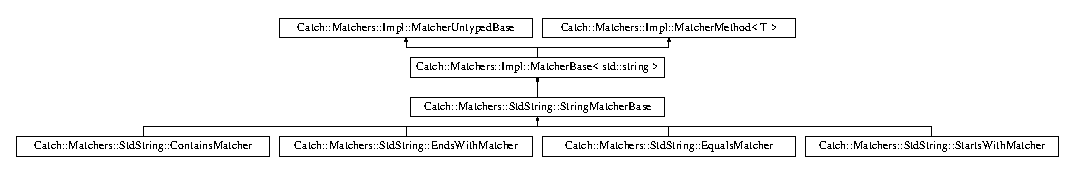
\includegraphics[height=1.879195cm]{struct_catch_1_1_matchers_1_1_std_string_1_1_string_matcher_base}
\end{center}
\end{figure}
\subsection*{Public Member Functions}
\begin{DoxyCompactItemize}
\item 
\mbox{\hyperlink{struct_catch_1_1_matchers_1_1_std_string_1_1_string_matcher_base_a3a9b66bae298ae27058478529b4bb39d}{String\+Matcher\+Base}} (std\+::string const \&operation, \mbox{\hyperlink{struct_catch_1_1_matchers_1_1_std_string_1_1_cased_string}{Cased\+String}} const \&comparator)
\item 
std\+::string \mbox{\hyperlink{struct_catch_1_1_matchers_1_1_std_string_1_1_string_matcher_base_a47af030f8cea42a601ffb1000eea5cca}{describe}} () const override
\end{DoxyCompactItemize}
\subsection*{Public Attributes}
\begin{DoxyCompactItemize}
\item 
\mbox{\hyperlink{struct_catch_1_1_matchers_1_1_std_string_1_1_cased_string}{Cased\+String}} \mbox{\hyperlink{struct_catch_1_1_matchers_1_1_std_string_1_1_string_matcher_base_a17c9f0fe40587070ffe998c193742831}{m\+\_\+comparator}}
\item 
std\+::string \mbox{\hyperlink{struct_catch_1_1_matchers_1_1_std_string_1_1_string_matcher_base_a7a25c4b7d863e9a1c406d81efd0f83ca}{m\+\_\+operation}}
\end{DoxyCompactItemize}
\subsection*{Additional Inherited Members}


\subsection{Detailed Description}


Definition at line 2379 of file catch.\+hpp.



\subsection{Constructor \& Destructor Documentation}
\mbox{\Hypertarget{struct_catch_1_1_matchers_1_1_std_string_1_1_string_matcher_base_a3a9b66bae298ae27058478529b4bb39d}\label{struct_catch_1_1_matchers_1_1_std_string_1_1_string_matcher_base_a3a9b66bae298ae27058478529b4bb39d}} 
\index{Catch\+::\+Matchers\+::\+Std\+String\+::\+String\+Matcher\+Base@{Catch\+::\+Matchers\+::\+Std\+String\+::\+String\+Matcher\+Base}!String\+Matcher\+Base@{String\+Matcher\+Base}}
\index{String\+Matcher\+Base@{String\+Matcher\+Base}!Catch\+::\+Matchers\+::\+Std\+String\+::\+String\+Matcher\+Base@{Catch\+::\+Matchers\+::\+Std\+String\+::\+String\+Matcher\+Base}}
\subsubsection{\texorpdfstring{String\+Matcher\+Base()}{StringMatcherBase()}}
{\footnotesize\ttfamily Catch\+::\+Matchers\+::\+Std\+String\+::\+String\+Matcher\+Base\+::\+String\+Matcher\+Base (\begin{DoxyParamCaption}\item[{std\+::string const \&}]{operation,  }\item[{\mbox{\hyperlink{struct_catch_1_1_matchers_1_1_std_string_1_1_cased_string}{Cased\+String}} const \&}]{comparator }\end{DoxyParamCaption})}



\subsection{Member Function Documentation}
\mbox{\Hypertarget{struct_catch_1_1_matchers_1_1_std_string_1_1_string_matcher_base_a47af030f8cea42a601ffb1000eea5cca}\label{struct_catch_1_1_matchers_1_1_std_string_1_1_string_matcher_base_a47af030f8cea42a601ffb1000eea5cca}} 
\index{Catch\+::\+Matchers\+::\+Std\+String\+::\+String\+Matcher\+Base@{Catch\+::\+Matchers\+::\+Std\+String\+::\+String\+Matcher\+Base}!describe@{describe}}
\index{describe@{describe}!Catch\+::\+Matchers\+::\+Std\+String\+::\+String\+Matcher\+Base@{Catch\+::\+Matchers\+::\+Std\+String\+::\+String\+Matcher\+Base}}
\subsubsection{\texorpdfstring{describe()}{describe()}}
{\footnotesize\ttfamily std\+::string Catch\+::\+Matchers\+::\+Std\+String\+::\+String\+Matcher\+Base\+::describe (\begin{DoxyParamCaption}{ }\end{DoxyParamCaption}) const\hspace{0.3cm}{\ttfamily [override]}, {\ttfamily [virtual]}}



Implements \mbox{\hyperlink{class_catch_1_1_matchers_1_1_impl_1_1_matcher_untyped_base_a91d3a907dbfcbb596077df24f6e11fe2}{Catch\+::\+Matchers\+::\+Impl\+::\+Matcher\+Untyped\+Base}}.



\subsection{Member Data Documentation}
\mbox{\Hypertarget{struct_catch_1_1_matchers_1_1_std_string_1_1_string_matcher_base_a17c9f0fe40587070ffe998c193742831}\label{struct_catch_1_1_matchers_1_1_std_string_1_1_string_matcher_base_a17c9f0fe40587070ffe998c193742831}} 
\index{Catch\+::\+Matchers\+::\+Std\+String\+::\+String\+Matcher\+Base@{Catch\+::\+Matchers\+::\+Std\+String\+::\+String\+Matcher\+Base}!m\+\_\+comparator@{m\+\_\+comparator}}
\index{m\+\_\+comparator@{m\+\_\+comparator}!Catch\+::\+Matchers\+::\+Std\+String\+::\+String\+Matcher\+Base@{Catch\+::\+Matchers\+::\+Std\+String\+::\+String\+Matcher\+Base}}
\subsubsection{\texorpdfstring{m\+\_\+comparator}{m\_comparator}}
{\footnotesize\ttfamily \mbox{\hyperlink{struct_catch_1_1_matchers_1_1_std_string_1_1_cased_string}{Cased\+String}} Catch\+::\+Matchers\+::\+Std\+String\+::\+String\+Matcher\+Base\+::m\+\_\+comparator}



Definition at line 2383 of file catch.\+hpp.

\mbox{\Hypertarget{struct_catch_1_1_matchers_1_1_std_string_1_1_string_matcher_base_a7a25c4b7d863e9a1c406d81efd0f83ca}\label{struct_catch_1_1_matchers_1_1_std_string_1_1_string_matcher_base_a7a25c4b7d863e9a1c406d81efd0f83ca}} 
\index{Catch\+::\+Matchers\+::\+Std\+String\+::\+String\+Matcher\+Base@{Catch\+::\+Matchers\+::\+Std\+String\+::\+String\+Matcher\+Base}!m\+\_\+operation@{m\+\_\+operation}}
\index{m\+\_\+operation@{m\+\_\+operation}!Catch\+::\+Matchers\+::\+Std\+String\+::\+String\+Matcher\+Base@{Catch\+::\+Matchers\+::\+Std\+String\+::\+String\+Matcher\+Base}}
\subsubsection{\texorpdfstring{m\+\_\+operation}{m\_operation}}
{\footnotesize\ttfamily std\+::string Catch\+::\+Matchers\+::\+Std\+String\+::\+String\+Matcher\+Base\+::m\+\_\+operation}



Definition at line 2384 of file catch.\+hpp.



The documentation for this struct was generated from the following file\+:\begin{DoxyCompactItemize}
\item 
D\+:/c++/block\+\_\+matrix-\/master/block\+\_\+matrix-\/master/test/\mbox{\hyperlink{catch_8hpp}{catch.\+hpp}}\end{DoxyCompactItemize}

\hypertarget{class_catch_1_1_string_ref}{}\section{Catch\+:\+:String\+Ref Class Reference}
\label{class_catch_1_1_string_ref}\index{Catch\+::\+String\+Ref@{Catch\+::\+String\+Ref}}


{\ttfamily \#include $<$catch.\+hpp$>$}

\subsection*{Public Types}
\begin{DoxyCompactItemize}
\item 
using \mbox{\hyperlink{class_catch_1_1_string_ref_a06b4db8fc82b197004291cf370b2ba7c}{size\+\_\+type}} = std\+::size\+\_\+t
\end{DoxyCompactItemize}
\subsection*{Public Member Functions}
\begin{DoxyCompactItemize}
\item 
\mbox{\hyperlink{class_catch_1_1_string_ref_a94319c75df6542327c93a312c6a80754}{String\+Ref}} () noexcept
\item 
\mbox{\hyperlink{class_catch_1_1_string_ref_a2f287267c3a988b288bfd910667c1cfc}{String\+Ref}} (\mbox{\hyperlink{class_catch_1_1_string_ref}{String\+Ref}} const \&other) noexcept
\item 
\mbox{\hyperlink{class_catch_1_1_string_ref_a407d5737b94e5a374add5c2794589733}{String\+Ref}} (\mbox{\hyperlink{class_catch_1_1_string_ref}{String\+Ref}} \&\&other) noexcept
\item 
\mbox{\hyperlink{class_catch_1_1_string_ref_aea45f5089c53adac362bff6bd7c40943}{String\+Ref}} (char const $\ast$raw\+Chars) noexcept
\item 
\mbox{\hyperlink{class_catch_1_1_string_ref_a320bf235274ebb90dd6af80485af2797}{String\+Ref}} (char const $\ast$raw\+Chars, \mbox{\hyperlink{class_catch_1_1_string_ref_a06b4db8fc82b197004291cf370b2ba7c}{size\+\_\+type}} \mbox{\hyperlink{class_catch_1_1_string_ref_ae084d72cb2952cee61a63ef36611d0ad}{size}}) noexcept
\item 
\mbox{\hyperlink{class_catch_1_1_string_ref_a7fe41469048f906e9a847798cd335f23}{String\+Ref}} (std\+::string const \&std\+String) noexcept
\item 
\mbox{\hyperlink{class_catch_1_1_string_ref_a387795c6d883d7281befe5e82920faf8}{$\sim$\+String\+Ref}} () noexcept
\item 
auto \mbox{\hyperlink{class_catch_1_1_string_ref_a14d5a1983e33c51c6b5fd33bffbebabb}{operator=}} (\mbox{\hyperlink{class_catch_1_1_string_ref}{String\+Ref}} const \&other) noexcept -\/$>$ \mbox{\hyperlink{class_catch_1_1_string_ref}{String\+Ref}} \&
\item 
\mbox{\hyperlink{class_catch_1_1_string_ref_ad9fde21785affacc32d7da7a70d74e93}{operator std\+::string}} () const
\item 
void \mbox{\hyperlink{class_catch_1_1_string_ref_a8a843e39ad3560d10a80524ed926ed63}{swap}} (\mbox{\hyperlink{class_catch_1_1_string_ref}{String\+Ref}} \&other) noexcept
\item 
auto \mbox{\hyperlink{class_catch_1_1_string_ref_aabb30149ab961187e4b3ff3394bf6e73}{operator==}} (\mbox{\hyperlink{class_catch_1_1_string_ref}{String\+Ref}} const \&other) const noexcept -\/$>$ bool
\item 
auto \mbox{\hyperlink{class_catch_1_1_string_ref_aaa6c8bf61c4628034c19763d1c8ad215}{operator!=}} (\mbox{\hyperlink{class_catch_1_1_string_ref}{String\+Ref}} const \&other) const noexcept -\/$>$ bool
\item 
auto \mbox{\hyperlink{class_catch_1_1_string_ref_a4ba2e01eec1f0f56c257d213c796ab3b}{operator\mbox{[}$\,$\mbox{]}}} (\mbox{\hyperlink{class_catch_1_1_string_ref_a06b4db8fc82b197004291cf370b2ba7c}{size\+\_\+type}} index) const noexcept -\/$>$ char
\item 
auto \mbox{\hyperlink{class_catch_1_1_string_ref_ac6b68b9dc1e1dec69e884e3f7be581bd}{empty}} () const noexcept -\/$>$ bool
\item 
auto \mbox{\hyperlink{class_catch_1_1_string_ref_ae084d72cb2952cee61a63ef36611d0ad}{size}} () const noexcept -\/$>$ \mbox{\hyperlink{class_catch_1_1_string_ref_a06b4db8fc82b197004291cf370b2ba7c}{size\+\_\+type}}
\item 
auto \mbox{\hyperlink{class_catch_1_1_string_ref_a6a6cac7430e626ffdd7550a081e8168f}{number\+Of\+Characters}} () const noexcept -\/$>$ \mbox{\hyperlink{class_catch_1_1_string_ref_a06b4db8fc82b197004291cf370b2ba7c}{size\+\_\+type}}
\item 
auto \mbox{\hyperlink{class_catch_1_1_string_ref_a1669cb2765e820ca258159676cbd82a5}{c\+\_\+str}} () const -\/$>$ char const $\ast$
\item 
auto \mbox{\hyperlink{class_catch_1_1_string_ref_a248568b467cf6599320903ae613c8eee}{substr}} (\mbox{\hyperlink{class_catch_1_1_string_ref_a06b4db8fc82b197004291cf370b2ba7c}{size\+\_\+type}} start, \mbox{\hyperlink{class_catch_1_1_string_ref_a06b4db8fc82b197004291cf370b2ba7c}{size\+\_\+type}} \mbox{\hyperlink{class_catch_1_1_string_ref_ae084d72cb2952cee61a63ef36611d0ad}{size}}) const noexcept -\/$>$ \mbox{\hyperlink{class_catch_1_1_string_ref}{String\+Ref}}
\item 
auto \mbox{\hyperlink{class_catch_1_1_string_ref_aee240387305ca8b249169d79f36e7002}{current\+Data}} () const noexcept -\/$>$ char const $\ast$
\end{DoxyCompactItemize}
\subsection*{Friends}
\begin{DoxyCompactItemize}
\item 
struct \mbox{\hyperlink{class_catch_1_1_string_ref_a420e64e1652de1b0d427775781b018f5}{String\+Ref\+Test\+Access}}
\end{DoxyCompactItemize}


\subsection{Detailed Description}
A non-\/owning string class (similar to the forthcoming std\+::string\+\_\+view) Note that, because a \mbox{\hyperlink{class_catch_1_1_string_ref}{String\+Ref}} may be a substring of another string, it may not be null terminated. \mbox{\hyperlink{class_catch_1_1_string_ref_a1669cb2765e820ca258159676cbd82a5}{c\+\_\+str()}} must return a null terminated string, however, and so the \mbox{\hyperlink{class_catch_1_1_string_ref}{String\+Ref}} will internally take ownership (taking a copy), if necessary. In theory this ownership is not externally visible -\/ but it does mean (substring) String\+Refs should not be shared between threads. 

Definition at line 377 of file catch.\+hpp.



\subsection{Member Typedef Documentation}
\mbox{\Hypertarget{class_catch_1_1_string_ref_a06b4db8fc82b197004291cf370b2ba7c}\label{class_catch_1_1_string_ref_a06b4db8fc82b197004291cf370b2ba7c}} 
\index{Catch\+::\+String\+Ref@{Catch\+::\+String\+Ref}!size\+\_\+type@{size\+\_\+type}}
\index{size\+\_\+type@{size\+\_\+type}!Catch\+::\+String\+Ref@{Catch\+::\+String\+Ref}}
\subsubsection{\texorpdfstring{size\+\_\+type}{size\_type}}
{\footnotesize\ttfamily using \mbox{\hyperlink{class_catch_1_1_string_ref_a06b4db8fc82b197004291cf370b2ba7c}{Catch\+::\+String\+Ref\+::size\+\_\+type}} =  std\+::size\+\_\+t}



Definition at line 379 of file catch.\+hpp.



\subsection{Constructor \& Destructor Documentation}
\mbox{\Hypertarget{class_catch_1_1_string_ref_a94319c75df6542327c93a312c6a80754}\label{class_catch_1_1_string_ref_a94319c75df6542327c93a312c6a80754}} 
\index{Catch\+::\+String\+Ref@{Catch\+::\+String\+Ref}!String\+Ref@{String\+Ref}}
\index{String\+Ref@{String\+Ref}!Catch\+::\+String\+Ref@{Catch\+::\+String\+Ref}}
\subsubsection{\texorpdfstring{String\+Ref()}{StringRef()}\hspace{0.1cm}{\footnotesize\ttfamily [1/6]}}
{\footnotesize\ttfamily Catch\+::\+String\+Ref\+::\+String\+Ref (\begin{DoxyParamCaption}{ }\end{DoxyParamCaption})\hspace{0.3cm}{\ttfamily [inline]}, {\ttfamily [noexcept]}}



Definition at line 394 of file catch.\+hpp.

\mbox{\Hypertarget{class_catch_1_1_string_ref_a2f287267c3a988b288bfd910667c1cfc}\label{class_catch_1_1_string_ref_a2f287267c3a988b288bfd910667c1cfc}} 
\index{Catch\+::\+String\+Ref@{Catch\+::\+String\+Ref}!String\+Ref@{String\+Ref}}
\index{String\+Ref@{String\+Ref}!Catch\+::\+String\+Ref@{Catch\+::\+String\+Ref}}
\subsubsection{\texorpdfstring{String\+Ref()}{StringRef()}\hspace{0.1cm}{\footnotesize\ttfamily [2/6]}}
{\footnotesize\ttfamily Catch\+::\+String\+Ref\+::\+String\+Ref (\begin{DoxyParamCaption}\item[{\mbox{\hyperlink{class_catch_1_1_string_ref}{String\+Ref}} const \&}]{other }\end{DoxyParamCaption})\hspace{0.3cm}{\ttfamily [inline]}, {\ttfamily [noexcept]}}



Definition at line 398 of file catch.\+hpp.

\mbox{\Hypertarget{class_catch_1_1_string_ref_a407d5737b94e5a374add5c2794589733}\label{class_catch_1_1_string_ref_a407d5737b94e5a374add5c2794589733}} 
\index{Catch\+::\+String\+Ref@{Catch\+::\+String\+Ref}!String\+Ref@{String\+Ref}}
\index{String\+Ref@{String\+Ref}!Catch\+::\+String\+Ref@{Catch\+::\+String\+Ref}}
\subsubsection{\texorpdfstring{String\+Ref()}{StringRef()}\hspace{0.1cm}{\footnotesize\ttfamily [3/6]}}
{\footnotesize\ttfamily Catch\+::\+String\+Ref\+::\+String\+Ref (\begin{DoxyParamCaption}\item[{\mbox{\hyperlink{class_catch_1_1_string_ref}{String\+Ref}} \&\&}]{other }\end{DoxyParamCaption})\hspace{0.3cm}{\ttfamily [inline]}, {\ttfamily [noexcept]}}



Definition at line 403 of file catch.\+hpp.

\mbox{\Hypertarget{class_catch_1_1_string_ref_aea45f5089c53adac362bff6bd7c40943}\label{class_catch_1_1_string_ref_aea45f5089c53adac362bff6bd7c40943}} 
\index{Catch\+::\+String\+Ref@{Catch\+::\+String\+Ref}!String\+Ref@{String\+Ref}}
\index{String\+Ref@{String\+Ref}!Catch\+::\+String\+Ref@{Catch\+::\+String\+Ref}}
\subsubsection{\texorpdfstring{String\+Ref()}{StringRef()}\hspace{0.1cm}{\footnotesize\ttfamily [4/6]}}
{\footnotesize\ttfamily Catch\+::\+String\+Ref\+::\+String\+Ref (\begin{DoxyParamCaption}\item[{char const $\ast$}]{raw\+Chars }\end{DoxyParamCaption})\hspace{0.3cm}{\ttfamily [noexcept]}}

\mbox{\Hypertarget{class_catch_1_1_string_ref_a320bf235274ebb90dd6af80485af2797}\label{class_catch_1_1_string_ref_a320bf235274ebb90dd6af80485af2797}} 
\index{Catch\+::\+String\+Ref@{Catch\+::\+String\+Ref}!String\+Ref@{String\+Ref}}
\index{String\+Ref@{String\+Ref}!Catch\+::\+String\+Ref@{Catch\+::\+String\+Ref}}
\subsubsection{\texorpdfstring{String\+Ref()}{StringRef()}\hspace{0.1cm}{\footnotesize\ttfamily [5/6]}}
{\footnotesize\ttfamily Catch\+::\+String\+Ref\+::\+String\+Ref (\begin{DoxyParamCaption}\item[{char const $\ast$}]{raw\+Chars,  }\item[{\mbox{\hyperlink{class_catch_1_1_string_ref_a06b4db8fc82b197004291cf370b2ba7c}{size\+\_\+type}}}]{size }\end{DoxyParamCaption})\hspace{0.3cm}{\ttfamily [inline]}, {\ttfamily [noexcept]}}



Definition at line 413 of file catch.\+hpp.

\mbox{\Hypertarget{class_catch_1_1_string_ref_a7fe41469048f906e9a847798cd335f23}\label{class_catch_1_1_string_ref_a7fe41469048f906e9a847798cd335f23}} 
\index{Catch\+::\+String\+Ref@{Catch\+::\+String\+Ref}!String\+Ref@{String\+Ref}}
\index{String\+Ref@{String\+Ref}!Catch\+::\+String\+Ref@{Catch\+::\+String\+Ref}}
\subsubsection{\texorpdfstring{String\+Ref()}{StringRef()}\hspace{0.1cm}{\footnotesize\ttfamily [6/6]}}
{\footnotesize\ttfamily Catch\+::\+String\+Ref\+::\+String\+Ref (\begin{DoxyParamCaption}\item[{std\+::string const \&}]{std\+String }\end{DoxyParamCaption})\hspace{0.3cm}{\ttfamily [inline]}, {\ttfamily [noexcept]}}



Definition at line 418 of file catch.\+hpp.

\mbox{\Hypertarget{class_catch_1_1_string_ref_a387795c6d883d7281befe5e82920faf8}\label{class_catch_1_1_string_ref_a387795c6d883d7281befe5e82920faf8}} 
\index{Catch\+::\+String\+Ref@{Catch\+::\+String\+Ref}!````~String\+Ref@{$\sim$\+String\+Ref}}
\index{````~String\+Ref@{$\sim$\+String\+Ref}!Catch\+::\+String\+Ref@{Catch\+::\+String\+Ref}}
\subsubsection{\texorpdfstring{$\sim$\+String\+Ref()}{~StringRef()}}
{\footnotesize\ttfamily Catch\+::\+String\+Ref\+::$\sim$\+String\+Ref (\begin{DoxyParamCaption}{ }\end{DoxyParamCaption})\hspace{0.3cm}{\ttfamily [inline]}, {\ttfamily [noexcept]}}



Definition at line 423 of file catch.\+hpp.



\subsection{Member Function Documentation}
\mbox{\Hypertarget{class_catch_1_1_string_ref_a1669cb2765e820ca258159676cbd82a5}\label{class_catch_1_1_string_ref_a1669cb2765e820ca258159676cbd82a5}} 
\index{Catch\+::\+String\+Ref@{Catch\+::\+String\+Ref}!c\+\_\+str@{c\+\_\+str}}
\index{c\+\_\+str@{c\+\_\+str}!Catch\+::\+String\+Ref@{Catch\+::\+String\+Ref}}
\subsubsection{\texorpdfstring{c\+\_\+str()}{c\_str()}}
{\footnotesize\ttfamily auto Catch\+::\+String\+Ref\+::c\+\_\+str (\begin{DoxyParamCaption}{ }\end{DoxyParamCaption}) const -\/$>$  char const $\ast$}

\mbox{\Hypertarget{class_catch_1_1_string_ref_aee240387305ca8b249169d79f36e7002}\label{class_catch_1_1_string_ref_aee240387305ca8b249169d79f36e7002}} 
\index{Catch\+::\+String\+Ref@{Catch\+::\+String\+Ref}!current\+Data@{current\+Data}}
\index{current\+Data@{current\+Data}!Catch\+::\+String\+Ref@{Catch\+::\+String\+Ref}}
\subsubsection{\texorpdfstring{current\+Data()}{currentData()}}
{\footnotesize\ttfamily auto Catch\+::\+String\+Ref\+::current\+Data (\begin{DoxyParamCaption}{ }\end{DoxyParamCaption}) const -\/$>$  char const $\ast$\hspace{0.3cm}{\ttfamily [noexcept]}}

\mbox{\Hypertarget{class_catch_1_1_string_ref_ac6b68b9dc1e1dec69e884e3f7be581bd}\label{class_catch_1_1_string_ref_ac6b68b9dc1e1dec69e884e3f7be581bd}} 
\index{Catch\+::\+String\+Ref@{Catch\+::\+String\+Ref}!empty@{empty}}
\index{empty@{empty}!Catch\+::\+String\+Ref@{Catch\+::\+String\+Ref}}
\subsubsection{\texorpdfstring{empty()}{empty()}}
{\footnotesize\ttfamily auto Catch\+::\+String\+Ref\+::empty (\begin{DoxyParamCaption}{ }\end{DoxyParamCaption}) const -\/$>$ bool \hspace{0.3cm}{\ttfamily [inline]}, {\ttfamily [noexcept]}}



Definition at line 446 of file catch.\+hpp.

\mbox{\Hypertarget{class_catch_1_1_string_ref_a6a6cac7430e626ffdd7550a081e8168f}\label{class_catch_1_1_string_ref_a6a6cac7430e626ffdd7550a081e8168f}} 
\index{Catch\+::\+String\+Ref@{Catch\+::\+String\+Ref}!number\+Of\+Characters@{number\+Of\+Characters}}
\index{number\+Of\+Characters@{number\+Of\+Characters}!Catch\+::\+String\+Ref@{Catch\+::\+String\+Ref}}
\subsubsection{\texorpdfstring{number\+Of\+Characters()}{numberOfCharacters()}}
{\footnotesize\ttfamily auto Catch\+::\+String\+Ref\+::number\+Of\+Characters (\begin{DoxyParamCaption}{ }\end{DoxyParamCaption}) const -\/$>$  \mbox{\hyperlink{class_catch_1_1_string_ref_a06b4db8fc82b197004291cf370b2ba7c}{size\+\_\+type}}\hspace{0.3cm}{\ttfamily [noexcept]}}

\mbox{\Hypertarget{class_catch_1_1_string_ref_ad9fde21785affacc32d7da7a70d74e93}\label{class_catch_1_1_string_ref_ad9fde21785affacc32d7da7a70d74e93}} 
\index{Catch\+::\+String\+Ref@{Catch\+::\+String\+Ref}!operator std\+::string@{operator std\+::string}}
\index{operator std\+::string@{operator std\+::string}!Catch\+::\+String\+Ref@{Catch\+::\+String\+Ref}}
\subsubsection{\texorpdfstring{operator std\+::string()}{operator std::string()}}
{\footnotesize\ttfamily Catch\+::\+String\+Ref\+::operator std\+::string (\begin{DoxyParamCaption}{ }\end{DoxyParamCaption}) const}

\mbox{\Hypertarget{class_catch_1_1_string_ref_aaa6c8bf61c4628034c19763d1c8ad215}\label{class_catch_1_1_string_ref_aaa6c8bf61c4628034c19763d1c8ad215}} 
\index{Catch\+::\+String\+Ref@{Catch\+::\+String\+Ref}!operator"!=@{operator"!=}}
\index{operator"!=@{operator"!=}!Catch\+::\+String\+Ref@{Catch\+::\+String\+Ref}}
\subsubsection{\texorpdfstring{operator"!=()}{operator!=()}}
{\footnotesize\ttfamily auto Catch\+::\+String\+Ref\+::operator!= (\begin{DoxyParamCaption}\item[{\mbox{\hyperlink{class_catch_1_1_string_ref}{String\+Ref}} const \&}]{other }\end{DoxyParamCaption}) const -\/$>$  bool\hspace{0.3cm}{\ttfamily [noexcept]}}

\mbox{\Hypertarget{class_catch_1_1_string_ref_a14d5a1983e33c51c6b5fd33bffbebabb}\label{class_catch_1_1_string_ref_a14d5a1983e33c51c6b5fd33bffbebabb}} 
\index{Catch\+::\+String\+Ref@{Catch\+::\+String\+Ref}!operator=@{operator=}}
\index{operator=@{operator=}!Catch\+::\+String\+Ref@{Catch\+::\+String\+Ref}}
\subsubsection{\texorpdfstring{operator=()}{operator=()}}
{\footnotesize\ttfamily auto Catch\+::\+String\+Ref\+::operator= (\begin{DoxyParamCaption}\item[{\mbox{\hyperlink{class_catch_1_1_string_ref}{String\+Ref}} const \&}]{other }\end{DoxyParamCaption}) -\/$>$ \mbox{\hyperlink{class_catch_1_1_string_ref}{String\+Ref}}\& \hspace{0.3cm}{\ttfamily [inline]}, {\ttfamily [noexcept]}}



Definition at line 427 of file catch.\+hpp.

\mbox{\Hypertarget{class_catch_1_1_string_ref_aabb30149ab961187e4b3ff3394bf6e73}\label{class_catch_1_1_string_ref_aabb30149ab961187e4b3ff3394bf6e73}} 
\index{Catch\+::\+String\+Ref@{Catch\+::\+String\+Ref}!operator==@{operator==}}
\index{operator==@{operator==}!Catch\+::\+String\+Ref@{Catch\+::\+String\+Ref}}
\subsubsection{\texorpdfstring{operator==()}{operator==()}}
{\footnotesize\ttfamily auto Catch\+::\+String\+Ref\+::operator== (\begin{DoxyParamCaption}\item[{\mbox{\hyperlink{class_catch_1_1_string_ref}{String\+Ref}} const \&}]{other }\end{DoxyParamCaption}) const -\/$>$  bool\hspace{0.3cm}{\ttfamily [noexcept]}}

\mbox{\Hypertarget{class_catch_1_1_string_ref_a4ba2e01eec1f0f56c257d213c796ab3b}\label{class_catch_1_1_string_ref_a4ba2e01eec1f0f56c257d213c796ab3b}} 
\index{Catch\+::\+String\+Ref@{Catch\+::\+String\+Ref}!operator\mbox{[}\mbox{]}@{operator[]}}
\index{operator\mbox{[}\mbox{]}@{operator[]}!Catch\+::\+String\+Ref@{Catch\+::\+String\+Ref}}
\subsubsection{\texorpdfstring{operator[]()}{operator[]()}}
{\footnotesize\ttfamily auto Catch\+::\+String\+Ref\+::operator\mbox{[}$\,$\mbox{]} (\begin{DoxyParamCaption}\item[{\mbox{\hyperlink{class_catch_1_1_string_ref_a06b4db8fc82b197004291cf370b2ba7c}{size\+\_\+type}}}]{index }\end{DoxyParamCaption}) const -\/$>$  char\hspace{0.3cm}{\ttfamily [noexcept]}}

\mbox{\Hypertarget{class_catch_1_1_string_ref_ae084d72cb2952cee61a63ef36611d0ad}\label{class_catch_1_1_string_ref_ae084d72cb2952cee61a63ef36611d0ad}} 
\index{Catch\+::\+String\+Ref@{Catch\+::\+String\+Ref}!size@{size}}
\index{size@{size}!Catch\+::\+String\+Ref@{Catch\+::\+String\+Ref}}
\subsubsection{\texorpdfstring{size()}{size()}}
{\footnotesize\ttfamily auto Catch\+::\+String\+Ref\+::size (\begin{DoxyParamCaption}{ }\end{DoxyParamCaption}) const -\/$>$ \mbox{\hyperlink{class_catch_1_1_string_ref_a06b4db8fc82b197004291cf370b2ba7c}{size\+\_\+type}} \hspace{0.3cm}{\ttfamily [inline]}, {\ttfamily [noexcept]}}



Definition at line 449 of file catch.\+hpp.

\mbox{\Hypertarget{class_catch_1_1_string_ref_a248568b467cf6599320903ae613c8eee}\label{class_catch_1_1_string_ref_a248568b467cf6599320903ae613c8eee}} 
\index{Catch\+::\+String\+Ref@{Catch\+::\+String\+Ref}!substr@{substr}}
\index{substr@{substr}!Catch\+::\+String\+Ref@{Catch\+::\+String\+Ref}}
\subsubsection{\texorpdfstring{substr()}{substr()}}
{\footnotesize\ttfamily auto Catch\+::\+String\+Ref\+::substr (\begin{DoxyParamCaption}\item[{\mbox{\hyperlink{class_catch_1_1_string_ref_a06b4db8fc82b197004291cf370b2ba7c}{size\+\_\+type}}}]{start,  }\item[{\mbox{\hyperlink{class_catch_1_1_string_ref_a06b4db8fc82b197004291cf370b2ba7c}{size\+\_\+type}}}]{size }\end{DoxyParamCaption}) const -\/$>$  \mbox{\hyperlink{class_catch_1_1_string_ref}{String\+Ref}}\hspace{0.3cm}{\ttfamily [noexcept]}}

\mbox{\Hypertarget{class_catch_1_1_string_ref_a8a843e39ad3560d10a80524ed926ed63}\label{class_catch_1_1_string_ref_a8a843e39ad3560d10a80524ed926ed63}} 
\index{Catch\+::\+String\+Ref@{Catch\+::\+String\+Ref}!swap@{swap}}
\index{swap@{swap}!Catch\+::\+String\+Ref@{Catch\+::\+String\+Ref}}
\subsubsection{\texorpdfstring{swap()}{swap()}}
{\footnotesize\ttfamily void Catch\+::\+String\+Ref\+::swap (\begin{DoxyParamCaption}\item[{\mbox{\hyperlink{class_catch_1_1_string_ref}{String\+Ref}} \&}]{other }\end{DoxyParamCaption})\hspace{0.3cm}{\ttfamily [noexcept]}}



\subsection{Friends And Related Function Documentation}
\mbox{\Hypertarget{class_catch_1_1_string_ref_a420e64e1652de1b0d427775781b018f5}\label{class_catch_1_1_string_ref_a420e64e1652de1b0d427775781b018f5}} 
\index{Catch\+::\+String\+Ref@{Catch\+::\+String\+Ref}!String\+Ref\+Test\+Access@{String\+Ref\+Test\+Access}}
\index{String\+Ref\+Test\+Access@{String\+Ref\+Test\+Access}!Catch\+::\+String\+Ref@{Catch\+::\+String\+Ref}}
\subsubsection{\texorpdfstring{String\+Ref\+Test\+Access}{StringRefTestAccess}}
{\footnotesize\ttfamily friend struct String\+Ref\+Test\+Access\hspace{0.3cm}{\ttfamily [friend]}}



Definition at line 382 of file catch.\+hpp.



The documentation for this class was generated from the following file\+:\begin{DoxyCompactItemize}
\item 
D\+:/c++/block\+\_\+matrix-\/master/block\+\_\+matrix-\/master/test/\mbox{\hyperlink{catch_8hpp}{catch.\+hpp}}\end{DoxyCompactItemize}

\hypertarget{class_catch_1_1_test_case}{}\section{Catch\+:\+:Test\+Case Class Reference}
\label{class_catch_1_1_test_case}\index{Catch\+::\+Test\+Case@{Catch\+::\+Test\+Case}}


{\ttfamily \#include $<$catch.\+hpp$>$}

Inheritance diagram for Catch\+:\+:Test\+Case\+:\begin{figure}[H]
\begin{center}
\leavevmode
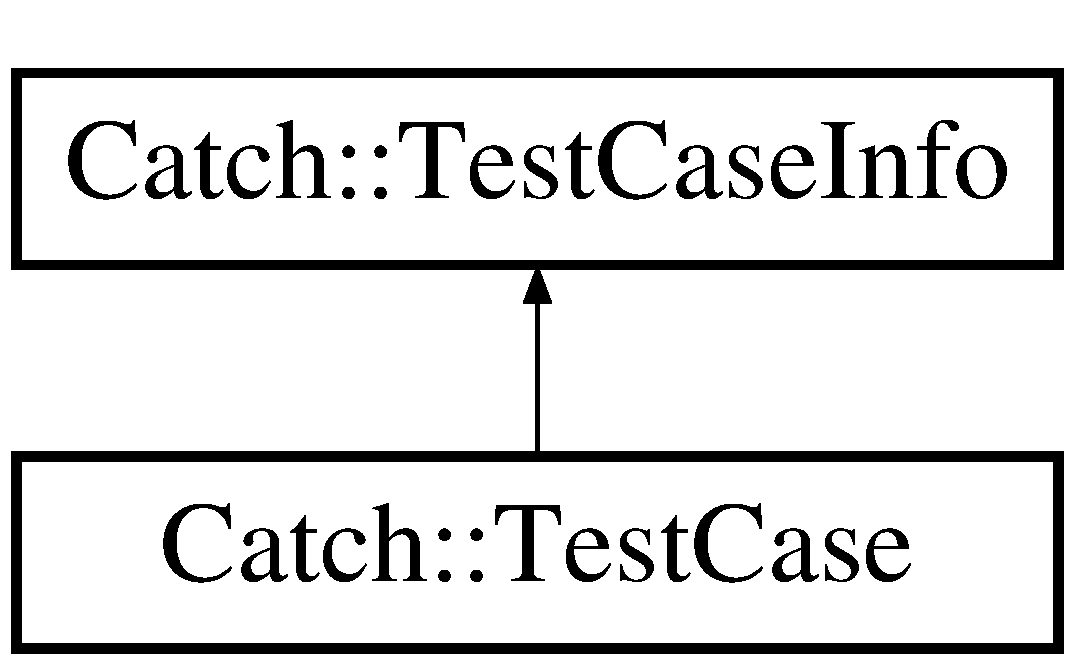
\includegraphics[height=2.000000cm]{class_catch_1_1_test_case}
\end{center}
\end{figure}
\subsection*{Public Member Functions}
\begin{DoxyCompactItemize}
\item 
\mbox{\hyperlink{class_catch_1_1_test_case_aae5709fc1cb68e19ab0ac27e1ffd6a76}{Test\+Case}} (\mbox{\hyperlink{struct_catch_1_1_i_test_invoker}{I\+Test\+Invoker}} $\ast$test\+Case, \mbox{\hyperlink{struct_catch_1_1_test_case_info}{Test\+Case\+Info}} \&\&info)
\item 
\mbox{\hyperlink{class_catch_1_1_test_case}{Test\+Case}} \mbox{\hyperlink{class_catch_1_1_test_case_a0812e8a216d09b087d5874687009f0d6}{with\+Name}} (std\+::string const \&\+\_\+new\+Name) const
\item 
void \mbox{\hyperlink{class_catch_1_1_test_case_a26f346c8446dded0562fe3818ae71651}{invoke}} () const
\item 
\mbox{\hyperlink{struct_catch_1_1_test_case_info}{Test\+Case\+Info}} const  \& \mbox{\hyperlink{class_catch_1_1_test_case_a1ea0d79f49156cebea076fe1ba50d2b6}{get\+Test\+Case\+Info}} () const
\item 
bool \mbox{\hyperlink{class_catch_1_1_test_case_a5456d03a90f75292835c158f3a3374a1}{operator==}} (\mbox{\hyperlink{class_catch_1_1_test_case}{Test\+Case}} const \&other) const
\item 
bool \mbox{\hyperlink{class_catch_1_1_test_case_a030e4b9282e9b32e08c8bd5e5cd6fa98}{operator$<$}} (\mbox{\hyperlink{class_catch_1_1_test_case}{Test\+Case}} const \&other) const
\end{DoxyCompactItemize}
\subsection*{Additional Inherited Members}


\subsection{Detailed Description}


Definition at line 2723 of file catch.\+hpp.



\subsection{Constructor \& Destructor Documentation}
\mbox{\Hypertarget{class_catch_1_1_test_case_aae5709fc1cb68e19ab0ac27e1ffd6a76}\label{class_catch_1_1_test_case_aae5709fc1cb68e19ab0ac27e1ffd6a76}} 
\index{Catch\+::\+Test\+Case@{Catch\+::\+Test\+Case}!Test\+Case@{Test\+Case}}
\index{Test\+Case@{Test\+Case}!Catch\+::\+Test\+Case@{Catch\+::\+Test\+Case}}
\subsubsection{\texorpdfstring{Test\+Case()}{TestCase()}}
{\footnotesize\ttfamily Catch\+::\+Test\+Case\+::\+Test\+Case (\begin{DoxyParamCaption}\item[{\mbox{\hyperlink{struct_catch_1_1_i_test_invoker}{I\+Test\+Invoker}} $\ast$}]{test\+Case,  }\item[{\mbox{\hyperlink{struct_catch_1_1_test_case_info}{Test\+Case\+Info}} \&\&}]{info }\end{DoxyParamCaption})}



\subsection{Member Function Documentation}
\mbox{\Hypertarget{class_catch_1_1_test_case_a1ea0d79f49156cebea076fe1ba50d2b6}\label{class_catch_1_1_test_case_a1ea0d79f49156cebea076fe1ba50d2b6}} 
\index{Catch\+::\+Test\+Case@{Catch\+::\+Test\+Case}!get\+Test\+Case\+Info@{get\+Test\+Case\+Info}}
\index{get\+Test\+Case\+Info@{get\+Test\+Case\+Info}!Catch\+::\+Test\+Case@{Catch\+::\+Test\+Case}}
\subsubsection{\texorpdfstring{get\+Test\+Case\+Info()}{getTestCaseInfo()}}
{\footnotesize\ttfamily \mbox{\hyperlink{struct_catch_1_1_test_case_info}{Test\+Case\+Info}} const\& Catch\+::\+Test\+Case\+::get\+Test\+Case\+Info (\begin{DoxyParamCaption}{ }\end{DoxyParamCaption}) const}

\mbox{\Hypertarget{class_catch_1_1_test_case_a26f346c8446dded0562fe3818ae71651}\label{class_catch_1_1_test_case_a26f346c8446dded0562fe3818ae71651}} 
\index{Catch\+::\+Test\+Case@{Catch\+::\+Test\+Case}!invoke@{invoke}}
\index{invoke@{invoke}!Catch\+::\+Test\+Case@{Catch\+::\+Test\+Case}}
\subsubsection{\texorpdfstring{invoke()}{invoke()}}
{\footnotesize\ttfamily void Catch\+::\+Test\+Case\+::invoke (\begin{DoxyParamCaption}{ }\end{DoxyParamCaption}) const}

\mbox{\Hypertarget{class_catch_1_1_test_case_a030e4b9282e9b32e08c8bd5e5cd6fa98}\label{class_catch_1_1_test_case_a030e4b9282e9b32e08c8bd5e5cd6fa98}} 
\index{Catch\+::\+Test\+Case@{Catch\+::\+Test\+Case}!operator$<$@{operator$<$}}
\index{operator$<$@{operator$<$}!Catch\+::\+Test\+Case@{Catch\+::\+Test\+Case}}
\subsubsection{\texorpdfstring{operator$<$()}{operator<()}}
{\footnotesize\ttfamily bool Catch\+::\+Test\+Case\+::operator$<$ (\begin{DoxyParamCaption}\item[{\mbox{\hyperlink{class_catch_1_1_test_case}{Test\+Case}} const \&}]{other }\end{DoxyParamCaption}) const}

\mbox{\Hypertarget{class_catch_1_1_test_case_a5456d03a90f75292835c158f3a3374a1}\label{class_catch_1_1_test_case_a5456d03a90f75292835c158f3a3374a1}} 
\index{Catch\+::\+Test\+Case@{Catch\+::\+Test\+Case}!operator==@{operator==}}
\index{operator==@{operator==}!Catch\+::\+Test\+Case@{Catch\+::\+Test\+Case}}
\subsubsection{\texorpdfstring{operator==()}{operator==()}}
{\footnotesize\ttfamily bool Catch\+::\+Test\+Case\+::operator== (\begin{DoxyParamCaption}\item[{\mbox{\hyperlink{class_catch_1_1_test_case}{Test\+Case}} const \&}]{other }\end{DoxyParamCaption}) const}

\mbox{\Hypertarget{class_catch_1_1_test_case_a0812e8a216d09b087d5874687009f0d6}\label{class_catch_1_1_test_case_a0812e8a216d09b087d5874687009f0d6}} 
\index{Catch\+::\+Test\+Case@{Catch\+::\+Test\+Case}!with\+Name@{with\+Name}}
\index{with\+Name@{with\+Name}!Catch\+::\+Test\+Case@{Catch\+::\+Test\+Case}}
\subsubsection{\texorpdfstring{with\+Name()}{withName()}}
{\footnotesize\ttfamily \mbox{\hyperlink{class_catch_1_1_test_case}{Test\+Case}} Catch\+::\+Test\+Case\+::with\+Name (\begin{DoxyParamCaption}\item[{std\+::string const \&}]{\+\_\+new\+Name }\end{DoxyParamCaption}) const}



The documentation for this class was generated from the following file\+:\begin{DoxyCompactItemize}
\item 
D\+:/c++/block\+\_\+matrix-\/master/block\+\_\+matrix-\/master/test/\mbox{\hyperlink{catch_8hpp}{catch.\+hpp}}\end{DoxyCompactItemize}

\hypertarget{struct_catch_1_1_test_case_info}{}\section{Catch\+:\+:Test\+Case\+Info Struct Reference}
\label{struct_catch_1_1_test_case_info}\index{Catch\+::\+Test\+Case\+Info@{Catch\+::\+Test\+Case\+Info}}


{\ttfamily \#include $<$catch.\+hpp$>$}

Inheritance diagram for Catch\+:\+:Test\+Case\+Info\+:\begin{figure}[H]
\begin{center}
\leavevmode
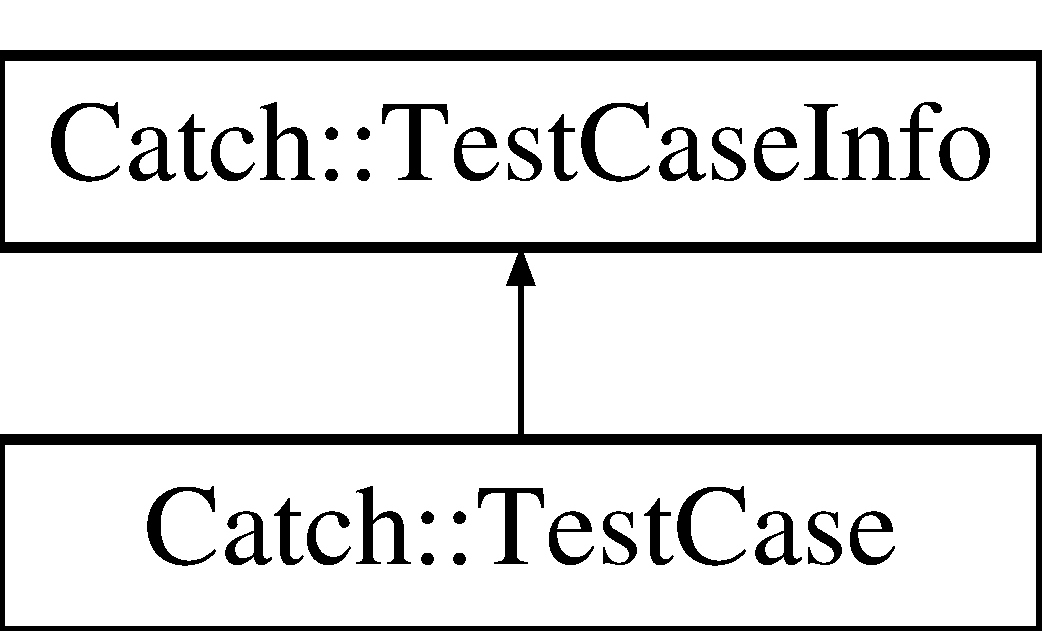
\includegraphics[height=2.000000cm]{struct_catch_1_1_test_case_info}
\end{center}
\end{figure}
\subsection*{Public Types}
\begin{DoxyCompactItemize}
\item 
enum \mbox{\hyperlink{struct_catch_1_1_test_case_info_a39b232f74b4a7a6f2183b96759027eac}{Special\+Properties}} \{ \newline
\mbox{\hyperlink{struct_catch_1_1_test_case_info_a39b232f74b4a7a6f2183b96759027eacaf94e9de5f8ec1e53b1aa761ec564b31a}{None}} = 0, 
\mbox{\hyperlink{struct_catch_1_1_test_case_info_a39b232f74b4a7a6f2183b96759027eacaeda53906c14c3973e0980900c132b8f7}{Is\+Hidden}} = 1 $<$$<$ 1, 
\mbox{\hyperlink{struct_catch_1_1_test_case_info_a39b232f74b4a7a6f2183b96759027eacaf9002285bccfc343935958f3953f4c01}{Should\+Fail}} = 1 $<$$<$ 2, 
\mbox{\hyperlink{struct_catch_1_1_test_case_info_a39b232f74b4a7a6f2183b96759027eacadf1873d3271121cb9f52d7df45b416ca}{May\+Fail}} = 1 $<$$<$ 3, 
\newline
\mbox{\hyperlink{struct_catch_1_1_test_case_info_a39b232f74b4a7a6f2183b96759027eaca4704adf89ed7f7ad653d08f99813a974}{Throws}} = 1 $<$$<$ 4, 
\mbox{\hyperlink{struct_catch_1_1_test_case_info_a39b232f74b4a7a6f2183b96759027eaca06472887b53fda9eb8015d74e7fd2cf1}{Non\+Portable}} = 1 $<$$<$ 5, 
\mbox{\hyperlink{struct_catch_1_1_test_case_info_a39b232f74b4a7a6f2183b96759027eacad0e25e337246ae34d555fe53baf81c16}{Benchmark}} = 1 $<$$<$ 6
 \}
\end{DoxyCompactItemize}
\subsection*{Public Member Functions}
\begin{DoxyCompactItemize}
\item 
\mbox{\hyperlink{struct_catch_1_1_test_case_info_ad1a6b08b5a83d1c5eb4596b727b5305f}{Test\+Case\+Info}} (std\+::string const \&\+\_\+name, std\+::string const \&\+\_\+class\+Name, std\+::string const \&\+\_\+description, std\+::vector$<$ std\+::string $>$ const \&\+\_\+tags, \mbox{\hyperlink{struct_catch_1_1_source_line_info}{Source\+Line\+Info}} const \&\+\_\+line\+Info)
\item 
bool \mbox{\hyperlink{struct_catch_1_1_test_case_info_a934b1a0952700743e99d62ec1731a2e2}{is\+Hidden}} () const
\item 
bool \mbox{\hyperlink{struct_catch_1_1_test_case_info_afc70d4379a2070cc22b693ffe3932c1a}{throws}} () const
\item 
bool \mbox{\hyperlink{struct_catch_1_1_test_case_info_a5f37291295e3a6de2dd85324c941edaf}{ok\+To\+Fail}} () const
\item 
bool \mbox{\hyperlink{struct_catch_1_1_test_case_info_abe33d81233230cdae8afa714688e905b}{expected\+To\+Fail}} () const
\item 
std\+::string \mbox{\hyperlink{struct_catch_1_1_test_case_info_a17506de67fb18e27511c17f8a81119d8}{tags\+As\+String}} () const
\end{DoxyCompactItemize}
\subsection*{Public Attributes}
\begin{DoxyCompactItemize}
\item 
std\+::string \mbox{\hyperlink{struct_catch_1_1_test_case_info_a463794e2f5cfead307c93efd134ade36}{name}}
\item 
std\+::string \mbox{\hyperlink{struct_catch_1_1_test_case_info_a1a5e0825132a38d091defdebbf2f8ce9}{class\+Name}}
\item 
std\+::string \mbox{\hyperlink{struct_catch_1_1_test_case_info_a37fe2db9425bc45f6a33893eac31198e}{description}}
\item 
std\+::vector$<$ std\+::string $>$ \mbox{\hyperlink{struct_catch_1_1_test_case_info_a150a7cbca1dd0c91799ccb14ff822eb0}{tags}}
\item 
std\+::vector$<$ std\+::string $>$ \mbox{\hyperlink{struct_catch_1_1_test_case_info_a844e3de9baf6e53cadfba9733c236bfe}{lcase\+Tags}}
\item 
\mbox{\hyperlink{struct_catch_1_1_source_line_info}{Source\+Line\+Info}} \mbox{\hyperlink{struct_catch_1_1_test_case_info_aa9407b7f442655b51a2aad24b3fa2fd3}{line\+Info}}
\item 
\mbox{\hyperlink{struct_catch_1_1_test_case_info_a39b232f74b4a7a6f2183b96759027eac}{Special\+Properties}} \mbox{\hyperlink{struct_catch_1_1_test_case_info_afc1e84bd7a2e180895a06d9131302af0}{properties}}
\end{DoxyCompactItemize}
\subsection*{Friends}
\begin{DoxyCompactItemize}
\item 
void \mbox{\hyperlink{struct_catch_1_1_test_case_info_a0fe44abaf18ae7c26f98a9fc2b08679c}{set\+Tags}} (\mbox{\hyperlink{struct_catch_1_1_test_case_info}{Test\+Case\+Info}} \&test\+Case\+Info, std\+::vector$<$ std\+::string $>$ \mbox{\hyperlink{struct_catch_1_1_test_case_info_a150a7cbca1dd0c91799ccb14ff822eb0}{tags}})
\end{DoxyCompactItemize}


\subsection{Detailed Description}


Definition at line 2688 of file catch.\+hpp.



\subsection{Member Enumeration Documentation}
\mbox{\Hypertarget{struct_catch_1_1_test_case_info_a39b232f74b4a7a6f2183b96759027eac}\label{struct_catch_1_1_test_case_info_a39b232f74b4a7a6f2183b96759027eac}} 
\index{Catch\+::\+Test\+Case\+Info@{Catch\+::\+Test\+Case\+Info}!Special\+Properties@{Special\+Properties}}
\index{Special\+Properties@{Special\+Properties}!Catch\+::\+Test\+Case\+Info@{Catch\+::\+Test\+Case\+Info}}
\subsubsection{\texorpdfstring{Special\+Properties}{SpecialProperties}}
{\footnotesize\ttfamily enum \mbox{\hyperlink{struct_catch_1_1_test_case_info_a39b232f74b4a7a6f2183b96759027eac}{Catch\+::\+Test\+Case\+Info\+::\+Special\+Properties}}}

\begin{DoxyEnumFields}{Enumerator}
\raisebox{\heightof{T}}[0pt][0pt]{\index{None@{None}!Catch\+::\+Test\+Case\+Info@{Catch\+::\+Test\+Case\+Info}}\index{Catch\+::\+Test\+Case\+Info@{Catch\+::\+Test\+Case\+Info}!None@{None}}}\mbox{\Hypertarget{struct_catch_1_1_test_case_info_a39b232f74b4a7a6f2183b96759027eacaf94e9de5f8ec1e53b1aa761ec564b31a}\label{struct_catch_1_1_test_case_info_a39b232f74b4a7a6f2183b96759027eacaf94e9de5f8ec1e53b1aa761ec564b31a}} 
None&\\
\hline

\raisebox{\heightof{T}}[0pt][0pt]{\index{Is\+Hidden@{Is\+Hidden}!Catch\+::\+Test\+Case\+Info@{Catch\+::\+Test\+Case\+Info}}\index{Catch\+::\+Test\+Case\+Info@{Catch\+::\+Test\+Case\+Info}!Is\+Hidden@{Is\+Hidden}}}\mbox{\Hypertarget{struct_catch_1_1_test_case_info_a39b232f74b4a7a6f2183b96759027eacaeda53906c14c3973e0980900c132b8f7}\label{struct_catch_1_1_test_case_info_a39b232f74b4a7a6f2183b96759027eacaeda53906c14c3973e0980900c132b8f7}} 
Is\+Hidden&\\
\hline

\raisebox{\heightof{T}}[0pt][0pt]{\index{Should\+Fail@{Should\+Fail}!Catch\+::\+Test\+Case\+Info@{Catch\+::\+Test\+Case\+Info}}\index{Catch\+::\+Test\+Case\+Info@{Catch\+::\+Test\+Case\+Info}!Should\+Fail@{Should\+Fail}}}\mbox{\Hypertarget{struct_catch_1_1_test_case_info_a39b232f74b4a7a6f2183b96759027eacaf9002285bccfc343935958f3953f4c01}\label{struct_catch_1_1_test_case_info_a39b232f74b4a7a6f2183b96759027eacaf9002285bccfc343935958f3953f4c01}} 
Should\+Fail&\\
\hline

\raisebox{\heightof{T}}[0pt][0pt]{\index{May\+Fail@{May\+Fail}!Catch\+::\+Test\+Case\+Info@{Catch\+::\+Test\+Case\+Info}}\index{Catch\+::\+Test\+Case\+Info@{Catch\+::\+Test\+Case\+Info}!May\+Fail@{May\+Fail}}}\mbox{\Hypertarget{struct_catch_1_1_test_case_info_a39b232f74b4a7a6f2183b96759027eacadf1873d3271121cb9f52d7df45b416ca}\label{struct_catch_1_1_test_case_info_a39b232f74b4a7a6f2183b96759027eacadf1873d3271121cb9f52d7df45b416ca}} 
May\+Fail&\\
\hline

\raisebox{\heightof{T}}[0pt][0pt]{\index{Throws@{Throws}!Catch\+::\+Test\+Case\+Info@{Catch\+::\+Test\+Case\+Info}}\index{Catch\+::\+Test\+Case\+Info@{Catch\+::\+Test\+Case\+Info}!Throws@{Throws}}}\mbox{\Hypertarget{struct_catch_1_1_test_case_info_a39b232f74b4a7a6f2183b96759027eaca4704adf89ed7f7ad653d08f99813a974}\label{struct_catch_1_1_test_case_info_a39b232f74b4a7a6f2183b96759027eaca4704adf89ed7f7ad653d08f99813a974}} 
Throws&\\
\hline

\raisebox{\heightof{T}}[0pt][0pt]{\index{Non\+Portable@{Non\+Portable}!Catch\+::\+Test\+Case\+Info@{Catch\+::\+Test\+Case\+Info}}\index{Catch\+::\+Test\+Case\+Info@{Catch\+::\+Test\+Case\+Info}!Non\+Portable@{Non\+Portable}}}\mbox{\Hypertarget{struct_catch_1_1_test_case_info_a39b232f74b4a7a6f2183b96759027eaca06472887b53fda9eb8015d74e7fd2cf1}\label{struct_catch_1_1_test_case_info_a39b232f74b4a7a6f2183b96759027eaca06472887b53fda9eb8015d74e7fd2cf1}} 
Non\+Portable&\\
\hline

\raisebox{\heightof{T}}[0pt][0pt]{\index{Benchmark@{Benchmark}!Catch\+::\+Test\+Case\+Info@{Catch\+::\+Test\+Case\+Info}}\index{Catch\+::\+Test\+Case\+Info@{Catch\+::\+Test\+Case\+Info}!Benchmark@{Benchmark}}}\mbox{\Hypertarget{struct_catch_1_1_test_case_info_a39b232f74b4a7a6f2183b96759027eacad0e25e337246ae34d555fe53baf81c16}\label{struct_catch_1_1_test_case_info_a39b232f74b4a7a6f2183b96759027eacad0e25e337246ae34d555fe53baf81c16}} 
Benchmark&\\
\hline

\end{DoxyEnumFields}


Definition at line 2689 of file catch.\+hpp.



\subsection{Constructor \& Destructor Documentation}
\mbox{\Hypertarget{struct_catch_1_1_test_case_info_ad1a6b08b5a83d1c5eb4596b727b5305f}\label{struct_catch_1_1_test_case_info_ad1a6b08b5a83d1c5eb4596b727b5305f}} 
\index{Catch\+::\+Test\+Case\+Info@{Catch\+::\+Test\+Case\+Info}!Test\+Case\+Info@{Test\+Case\+Info}}
\index{Test\+Case\+Info@{Test\+Case\+Info}!Catch\+::\+Test\+Case\+Info@{Catch\+::\+Test\+Case\+Info}}
\subsubsection{\texorpdfstring{Test\+Case\+Info()}{TestCaseInfo()}}
{\footnotesize\ttfamily Catch\+::\+Test\+Case\+Info\+::\+Test\+Case\+Info (\begin{DoxyParamCaption}\item[{std\+::string const \&}]{\+\_\+name,  }\item[{std\+::string const \&}]{\+\_\+class\+Name,  }\item[{std\+::string const \&}]{\+\_\+description,  }\item[{std\+::vector$<$ std\+::string $>$ const \&}]{\+\_\+tags,  }\item[{\mbox{\hyperlink{struct_catch_1_1_source_line_info}{Source\+Line\+Info}} const \&}]{\+\_\+line\+Info }\end{DoxyParamCaption})}



\subsection{Member Function Documentation}
\mbox{\Hypertarget{struct_catch_1_1_test_case_info_abe33d81233230cdae8afa714688e905b}\label{struct_catch_1_1_test_case_info_abe33d81233230cdae8afa714688e905b}} 
\index{Catch\+::\+Test\+Case\+Info@{Catch\+::\+Test\+Case\+Info}!expected\+To\+Fail@{expected\+To\+Fail}}
\index{expected\+To\+Fail@{expected\+To\+Fail}!Catch\+::\+Test\+Case\+Info@{Catch\+::\+Test\+Case\+Info}}
\subsubsection{\texorpdfstring{expected\+To\+Fail()}{expectedToFail()}}
{\footnotesize\ttfamily bool Catch\+::\+Test\+Case\+Info\+::expected\+To\+Fail (\begin{DoxyParamCaption}{ }\end{DoxyParamCaption}) const}

\mbox{\Hypertarget{struct_catch_1_1_test_case_info_a934b1a0952700743e99d62ec1731a2e2}\label{struct_catch_1_1_test_case_info_a934b1a0952700743e99d62ec1731a2e2}} 
\index{Catch\+::\+Test\+Case\+Info@{Catch\+::\+Test\+Case\+Info}!is\+Hidden@{is\+Hidden}}
\index{is\+Hidden@{is\+Hidden}!Catch\+::\+Test\+Case\+Info@{Catch\+::\+Test\+Case\+Info}}
\subsubsection{\texorpdfstring{is\+Hidden()}{isHidden()}}
{\footnotesize\ttfamily bool Catch\+::\+Test\+Case\+Info\+::is\+Hidden (\begin{DoxyParamCaption}{ }\end{DoxyParamCaption}) const}

\mbox{\Hypertarget{struct_catch_1_1_test_case_info_a5f37291295e3a6de2dd85324c941edaf}\label{struct_catch_1_1_test_case_info_a5f37291295e3a6de2dd85324c941edaf}} 
\index{Catch\+::\+Test\+Case\+Info@{Catch\+::\+Test\+Case\+Info}!ok\+To\+Fail@{ok\+To\+Fail}}
\index{ok\+To\+Fail@{ok\+To\+Fail}!Catch\+::\+Test\+Case\+Info@{Catch\+::\+Test\+Case\+Info}}
\subsubsection{\texorpdfstring{ok\+To\+Fail()}{okToFail()}}
{\footnotesize\ttfamily bool Catch\+::\+Test\+Case\+Info\+::ok\+To\+Fail (\begin{DoxyParamCaption}{ }\end{DoxyParamCaption}) const}

\mbox{\Hypertarget{struct_catch_1_1_test_case_info_a17506de67fb18e27511c17f8a81119d8}\label{struct_catch_1_1_test_case_info_a17506de67fb18e27511c17f8a81119d8}} 
\index{Catch\+::\+Test\+Case\+Info@{Catch\+::\+Test\+Case\+Info}!tags\+As\+String@{tags\+As\+String}}
\index{tags\+As\+String@{tags\+As\+String}!Catch\+::\+Test\+Case\+Info@{Catch\+::\+Test\+Case\+Info}}
\subsubsection{\texorpdfstring{tags\+As\+String()}{tagsAsString()}}
{\footnotesize\ttfamily std\+::string Catch\+::\+Test\+Case\+Info\+::tags\+As\+String (\begin{DoxyParamCaption}{ }\end{DoxyParamCaption}) const}

\mbox{\Hypertarget{struct_catch_1_1_test_case_info_afc70d4379a2070cc22b693ffe3932c1a}\label{struct_catch_1_1_test_case_info_afc70d4379a2070cc22b693ffe3932c1a}} 
\index{Catch\+::\+Test\+Case\+Info@{Catch\+::\+Test\+Case\+Info}!throws@{throws}}
\index{throws@{throws}!Catch\+::\+Test\+Case\+Info@{Catch\+::\+Test\+Case\+Info}}
\subsubsection{\texorpdfstring{throws()}{throws()}}
{\footnotesize\ttfamily bool Catch\+::\+Test\+Case\+Info\+::throws (\begin{DoxyParamCaption}{ }\end{DoxyParamCaption}) const}



\subsection{Friends And Related Function Documentation}
\mbox{\Hypertarget{struct_catch_1_1_test_case_info_a0fe44abaf18ae7c26f98a9fc2b08679c}\label{struct_catch_1_1_test_case_info_a0fe44abaf18ae7c26f98a9fc2b08679c}} 
\index{Catch\+::\+Test\+Case\+Info@{Catch\+::\+Test\+Case\+Info}!set\+Tags@{set\+Tags}}
\index{set\+Tags@{set\+Tags}!Catch\+::\+Test\+Case\+Info@{Catch\+::\+Test\+Case\+Info}}
\subsubsection{\texorpdfstring{set\+Tags}{setTags}}
{\footnotesize\ttfamily void set\+Tags (\begin{DoxyParamCaption}\item[{\mbox{\hyperlink{struct_catch_1_1_test_case_info}{Test\+Case\+Info}} \&}]{test\+Case\+Info,  }\item[{std\+::vector$<$ std\+::string $>$}]{tags }\end{DoxyParamCaption})\hspace{0.3cm}{\ttfamily [friend]}}



\subsection{Member Data Documentation}
\mbox{\Hypertarget{struct_catch_1_1_test_case_info_a1a5e0825132a38d091defdebbf2f8ce9}\label{struct_catch_1_1_test_case_info_a1a5e0825132a38d091defdebbf2f8ce9}} 
\index{Catch\+::\+Test\+Case\+Info@{Catch\+::\+Test\+Case\+Info}!class\+Name@{class\+Name}}
\index{class\+Name@{class\+Name}!Catch\+::\+Test\+Case\+Info@{Catch\+::\+Test\+Case\+Info}}
\subsubsection{\texorpdfstring{class\+Name}{className}}
{\footnotesize\ttfamily std\+::string Catch\+::\+Test\+Case\+Info\+::class\+Name}



Definition at line 2715 of file catch.\+hpp.

\mbox{\Hypertarget{struct_catch_1_1_test_case_info_a37fe2db9425bc45f6a33893eac31198e}\label{struct_catch_1_1_test_case_info_a37fe2db9425bc45f6a33893eac31198e}} 
\index{Catch\+::\+Test\+Case\+Info@{Catch\+::\+Test\+Case\+Info}!description@{description}}
\index{description@{description}!Catch\+::\+Test\+Case\+Info@{Catch\+::\+Test\+Case\+Info}}
\subsubsection{\texorpdfstring{description}{description}}
{\footnotesize\ttfamily std\+::string Catch\+::\+Test\+Case\+Info\+::description}



Definition at line 2716 of file catch.\+hpp.

\mbox{\Hypertarget{struct_catch_1_1_test_case_info_a844e3de9baf6e53cadfba9733c236bfe}\label{struct_catch_1_1_test_case_info_a844e3de9baf6e53cadfba9733c236bfe}} 
\index{Catch\+::\+Test\+Case\+Info@{Catch\+::\+Test\+Case\+Info}!lcase\+Tags@{lcase\+Tags}}
\index{lcase\+Tags@{lcase\+Tags}!Catch\+::\+Test\+Case\+Info@{Catch\+::\+Test\+Case\+Info}}
\subsubsection{\texorpdfstring{lcase\+Tags}{lcaseTags}}
{\footnotesize\ttfamily std\+::vector$<$std\+::string$>$ Catch\+::\+Test\+Case\+Info\+::lcase\+Tags}



Definition at line 2718 of file catch.\+hpp.

\mbox{\Hypertarget{struct_catch_1_1_test_case_info_aa9407b7f442655b51a2aad24b3fa2fd3}\label{struct_catch_1_1_test_case_info_aa9407b7f442655b51a2aad24b3fa2fd3}} 
\index{Catch\+::\+Test\+Case\+Info@{Catch\+::\+Test\+Case\+Info}!line\+Info@{line\+Info}}
\index{line\+Info@{line\+Info}!Catch\+::\+Test\+Case\+Info@{Catch\+::\+Test\+Case\+Info}}
\subsubsection{\texorpdfstring{line\+Info}{lineInfo}}
{\footnotesize\ttfamily \mbox{\hyperlink{struct_catch_1_1_source_line_info}{Source\+Line\+Info}} Catch\+::\+Test\+Case\+Info\+::line\+Info}



Definition at line 2719 of file catch.\+hpp.

\mbox{\Hypertarget{struct_catch_1_1_test_case_info_a463794e2f5cfead307c93efd134ade36}\label{struct_catch_1_1_test_case_info_a463794e2f5cfead307c93efd134ade36}} 
\index{Catch\+::\+Test\+Case\+Info@{Catch\+::\+Test\+Case\+Info}!name@{name}}
\index{name@{name}!Catch\+::\+Test\+Case\+Info@{Catch\+::\+Test\+Case\+Info}}
\subsubsection{\texorpdfstring{name}{name}}
{\footnotesize\ttfamily std\+::string Catch\+::\+Test\+Case\+Info\+::name}



Definition at line 2714 of file catch.\+hpp.

\mbox{\Hypertarget{struct_catch_1_1_test_case_info_afc1e84bd7a2e180895a06d9131302af0}\label{struct_catch_1_1_test_case_info_afc1e84bd7a2e180895a06d9131302af0}} 
\index{Catch\+::\+Test\+Case\+Info@{Catch\+::\+Test\+Case\+Info}!properties@{properties}}
\index{properties@{properties}!Catch\+::\+Test\+Case\+Info@{Catch\+::\+Test\+Case\+Info}}
\subsubsection{\texorpdfstring{properties}{properties}}
{\footnotesize\ttfamily \mbox{\hyperlink{struct_catch_1_1_test_case_info_a39b232f74b4a7a6f2183b96759027eac}{Special\+Properties}} Catch\+::\+Test\+Case\+Info\+::properties}



Definition at line 2720 of file catch.\+hpp.

\mbox{\Hypertarget{struct_catch_1_1_test_case_info_a150a7cbca1dd0c91799ccb14ff822eb0}\label{struct_catch_1_1_test_case_info_a150a7cbca1dd0c91799ccb14ff822eb0}} 
\index{Catch\+::\+Test\+Case\+Info@{Catch\+::\+Test\+Case\+Info}!tags@{tags}}
\index{tags@{tags}!Catch\+::\+Test\+Case\+Info@{Catch\+::\+Test\+Case\+Info}}
\subsubsection{\texorpdfstring{tags}{tags}}
{\footnotesize\ttfamily std\+::vector$<$std\+::string$>$ Catch\+::\+Test\+Case\+Info\+::tags}



Definition at line 2717 of file catch.\+hpp.



The documentation for this struct was generated from the following file\+:\begin{DoxyCompactItemize}
\item 
D\+:/c++/block\+\_\+matrix-\/master/block\+\_\+matrix-\/master/test/\mbox{\hyperlink{catch_8hpp}{catch.\+hpp}}\end{DoxyCompactItemize}

\hypertarget{struct_catch_1_1_test_failure_exception}{}\section{Catch\+:\+:Test\+Failure\+Exception Struct Reference}
\label{struct_catch_1_1_test_failure_exception}\index{Catch\+::\+Test\+Failure\+Exception@{Catch\+::\+Test\+Failure\+Exception}}


{\ttfamily \#include $<$catch.\+hpp$>$}



\subsection{Detailed Description}


Definition at line 1476 of file catch.\+hpp.



The documentation for this struct was generated from the following file\+:\begin{DoxyCompactItemize}
\item 
D\+:/c++/block\+\_\+matrix-\/master/block\+\_\+matrix-\/master/test/\mbox{\hyperlink{catch_8hpp}{catch.\+hpp}}\end{DoxyCompactItemize}

\hypertarget{class_catch_1_1_test_invoker_as_method}{}\section{Catch\+:\+:Test\+Invoker\+As\+Method$<$ C $>$ Class Template Reference}
\label{class_catch_1_1_test_invoker_as_method}\index{Catch\+::\+Test\+Invoker\+As\+Method$<$ C $>$@{Catch\+::\+Test\+Invoker\+As\+Method$<$ C $>$}}


{\ttfamily \#include $<$catch.\+hpp$>$}

Inheritance diagram for Catch\+:\+:Test\+Invoker\+As\+Method$<$ C $>$\+:\begin{figure}[H]
\begin{center}
\leavevmode
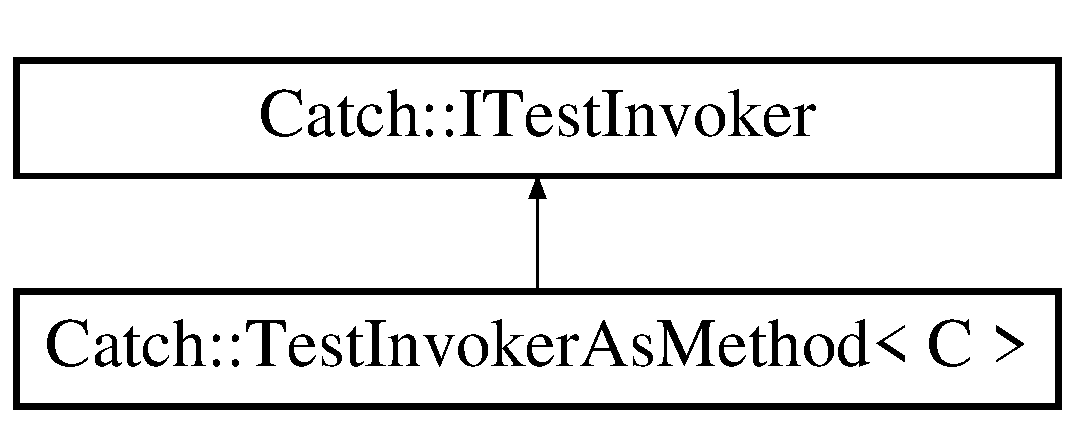
\includegraphics[height=2.000000cm]{class_catch_1_1_test_invoker_as_method}
\end{center}
\end{figure}
\subsection*{Public Member Functions}
\begin{DoxyCompactItemize}
\item 
\mbox{\hyperlink{class_catch_1_1_test_invoker_as_method_a119c4bdbbdd95c42859c18541987a1a4}{Test\+Invoker\+As\+Method}} (void(C\+::$\ast$test\+As\+Method)()) noexcept
\item 
void \mbox{\hyperlink{class_catch_1_1_test_invoker_as_method_a8115a06efe273f4112ec0b5452c1b5f2}{invoke}} () const override
\end{DoxyCompactItemize}


\subsection{Detailed Description}
\subsubsection*{template$<$typename C$>$\newline
class Catch\+::\+Test\+Invoker\+As\+Method$<$ C $>$}



Definition at line 485 of file catch.\+hpp.



\subsection{Constructor \& Destructor Documentation}
\mbox{\Hypertarget{class_catch_1_1_test_invoker_as_method_a119c4bdbbdd95c42859c18541987a1a4}\label{class_catch_1_1_test_invoker_as_method_a119c4bdbbdd95c42859c18541987a1a4}} 
\index{Catch\+::\+Test\+Invoker\+As\+Method@{Catch\+::\+Test\+Invoker\+As\+Method}!Test\+Invoker\+As\+Method@{Test\+Invoker\+As\+Method}}
\index{Test\+Invoker\+As\+Method@{Test\+Invoker\+As\+Method}!Catch\+::\+Test\+Invoker\+As\+Method@{Catch\+::\+Test\+Invoker\+As\+Method}}
\subsubsection{\texorpdfstring{Test\+Invoker\+As\+Method()}{TestInvokerAsMethod()}}
{\footnotesize\ttfamily template$<$typename C $>$ \\
\mbox{\hyperlink{class_catch_1_1_test_invoker_as_method}{Catch\+::\+Test\+Invoker\+As\+Method}}$<$ C $>$\+::\mbox{\hyperlink{class_catch_1_1_test_invoker_as_method}{Test\+Invoker\+As\+Method}} (\begin{DoxyParamCaption}\item[{void(C\+::$\ast$)()}]{test\+As\+Method }\end{DoxyParamCaption})\hspace{0.3cm}{\ttfamily [inline]}, {\ttfamily [noexcept]}}



Definition at line 488 of file catch.\+hpp.



\subsection{Member Function Documentation}
\mbox{\Hypertarget{class_catch_1_1_test_invoker_as_method_a8115a06efe273f4112ec0b5452c1b5f2}\label{class_catch_1_1_test_invoker_as_method_a8115a06efe273f4112ec0b5452c1b5f2}} 
\index{Catch\+::\+Test\+Invoker\+As\+Method@{Catch\+::\+Test\+Invoker\+As\+Method}!invoke@{invoke}}
\index{invoke@{invoke}!Catch\+::\+Test\+Invoker\+As\+Method@{Catch\+::\+Test\+Invoker\+As\+Method}}
\subsubsection{\texorpdfstring{invoke()}{invoke()}}
{\footnotesize\ttfamily template$<$typename C $>$ \\
void \mbox{\hyperlink{class_catch_1_1_test_invoker_as_method}{Catch\+::\+Test\+Invoker\+As\+Method}}$<$ C $>$\+::invoke (\begin{DoxyParamCaption}{ }\end{DoxyParamCaption}) const\hspace{0.3cm}{\ttfamily [inline]}, {\ttfamily [override]}, {\ttfamily [virtual]}}



Implements \mbox{\hyperlink{struct_catch_1_1_i_test_invoker_a6fcd5c5b67d6d5ade6491ff33411ca7f}{Catch\+::\+I\+Test\+Invoker}}.



Definition at line 490 of file catch.\+hpp.



The documentation for this class was generated from the following file\+:\begin{DoxyCompactItemize}
\item 
D\+:/c++/block\+\_\+matrix-\/master/block\+\_\+matrix-\/master/test/\mbox{\hyperlink{catch_8hpp}{catch.\+hpp}}\end{DoxyCompactItemize}

\hypertarget{class_catch_1_1_timer}{}\section{Catch\+:\+:Timer Class Reference}
\label{class_catch_1_1_timer}\index{Catch\+::\+Timer@{Catch\+::\+Timer}}


{\ttfamily \#include $<$catch.\+hpp$>$}

\subsection*{Public Member Functions}
\begin{DoxyCompactItemize}
\item 
void \mbox{\hyperlink{class_catch_1_1_timer_a0a56e879e43f36c102bf9ea8b5fc8b72}{start}} ()
\item 
auto \mbox{\hyperlink{class_catch_1_1_timer_a57be5d17ca868a2d6fb1eea84de665cf}{get\+Elapsed\+Nanoseconds}} () const -\/$>$ uint64\+\_\+t
\item 
auto \mbox{\hyperlink{class_catch_1_1_timer_a545de17a61a6fee1dbe3de5b0723e5fa}{get\+Elapsed\+Microseconds}} () const -\/$>$ uint64\+\_\+t
\item 
auto \mbox{\hyperlink{class_catch_1_1_timer_a30aaf458dbb59dd8ac8971c9c62e0eac}{get\+Elapsed\+Milliseconds}} () const -\/$>$ unsigned int
\item 
auto \mbox{\hyperlink{class_catch_1_1_timer_a065e37e3c9eb16bd4dcf41971d8deedc}{get\+Elapsed\+Seconds}} () const -\/$>$ double
\end{DoxyCompactItemize}


\subsection{Detailed Description}


Definition at line 1810 of file catch.\+hpp.



\subsection{Member Function Documentation}
\mbox{\Hypertarget{class_catch_1_1_timer_a545de17a61a6fee1dbe3de5b0723e5fa}\label{class_catch_1_1_timer_a545de17a61a6fee1dbe3de5b0723e5fa}} 
\index{Catch\+::\+Timer@{Catch\+::\+Timer}!get\+Elapsed\+Microseconds@{get\+Elapsed\+Microseconds}}
\index{get\+Elapsed\+Microseconds@{get\+Elapsed\+Microseconds}!Catch\+::\+Timer@{Catch\+::\+Timer}}
\subsubsection{\texorpdfstring{get\+Elapsed\+Microseconds()}{getElapsedMicroseconds()}}
{\footnotesize\ttfamily auto Catch\+::\+Timer\+::get\+Elapsed\+Microseconds (\begin{DoxyParamCaption}{ }\end{DoxyParamCaption}) const -\/$>$  uint64\+\_\+t}

\mbox{\Hypertarget{class_catch_1_1_timer_a30aaf458dbb59dd8ac8971c9c62e0eac}\label{class_catch_1_1_timer_a30aaf458dbb59dd8ac8971c9c62e0eac}} 
\index{Catch\+::\+Timer@{Catch\+::\+Timer}!get\+Elapsed\+Milliseconds@{get\+Elapsed\+Milliseconds}}
\index{get\+Elapsed\+Milliseconds@{get\+Elapsed\+Milliseconds}!Catch\+::\+Timer@{Catch\+::\+Timer}}
\subsubsection{\texorpdfstring{get\+Elapsed\+Milliseconds()}{getElapsedMilliseconds()}}
{\footnotesize\ttfamily auto Catch\+::\+Timer\+::get\+Elapsed\+Milliseconds (\begin{DoxyParamCaption}{ }\end{DoxyParamCaption}) const -\/$>$  unsigned int}

\mbox{\Hypertarget{class_catch_1_1_timer_a57be5d17ca868a2d6fb1eea84de665cf}\label{class_catch_1_1_timer_a57be5d17ca868a2d6fb1eea84de665cf}} 
\index{Catch\+::\+Timer@{Catch\+::\+Timer}!get\+Elapsed\+Nanoseconds@{get\+Elapsed\+Nanoseconds}}
\index{get\+Elapsed\+Nanoseconds@{get\+Elapsed\+Nanoseconds}!Catch\+::\+Timer@{Catch\+::\+Timer}}
\subsubsection{\texorpdfstring{get\+Elapsed\+Nanoseconds()}{getElapsedNanoseconds()}}
{\footnotesize\ttfamily auto Catch\+::\+Timer\+::get\+Elapsed\+Nanoseconds (\begin{DoxyParamCaption}{ }\end{DoxyParamCaption}) const -\/$>$  uint64\+\_\+t}

\mbox{\Hypertarget{class_catch_1_1_timer_a065e37e3c9eb16bd4dcf41971d8deedc}\label{class_catch_1_1_timer_a065e37e3c9eb16bd4dcf41971d8deedc}} 
\index{Catch\+::\+Timer@{Catch\+::\+Timer}!get\+Elapsed\+Seconds@{get\+Elapsed\+Seconds}}
\index{get\+Elapsed\+Seconds@{get\+Elapsed\+Seconds}!Catch\+::\+Timer@{Catch\+::\+Timer}}
\subsubsection{\texorpdfstring{get\+Elapsed\+Seconds()}{getElapsedSeconds()}}
{\footnotesize\ttfamily auto Catch\+::\+Timer\+::get\+Elapsed\+Seconds (\begin{DoxyParamCaption}{ }\end{DoxyParamCaption}) const -\/$>$  double}

\mbox{\Hypertarget{class_catch_1_1_timer_a0a56e879e43f36c102bf9ea8b5fc8b72}\label{class_catch_1_1_timer_a0a56e879e43f36c102bf9ea8b5fc8b72}} 
\index{Catch\+::\+Timer@{Catch\+::\+Timer}!start@{start}}
\index{start@{start}!Catch\+::\+Timer@{Catch\+::\+Timer}}
\subsubsection{\texorpdfstring{start()}{start()}}
{\footnotesize\ttfamily void Catch\+::\+Timer\+::start (\begin{DoxyParamCaption}{ }\end{DoxyParamCaption})}



The documentation for this class was generated from the following file\+:\begin{DoxyCompactItemize}
\item 
D\+:/c++/block\+\_\+matrix-\/master/block\+\_\+matrix-\/master/test/\mbox{\hyperlink{catch_8hpp}{catch.\+hpp}}\end{DoxyCompactItemize}

\hypertarget{struct_catch_1_1_totals}{}\section{Catch\+:\+:Totals Struct Reference}
\label{struct_catch_1_1_totals}\index{Catch\+::\+Totals@{Catch\+::\+Totals}}


{\ttfamily \#include $<$catch.\+hpp$>$}

\subsection*{Public Member Functions}
\begin{DoxyCompactItemize}
\item 
\mbox{\hyperlink{struct_catch_1_1_totals}{Totals}} \mbox{\hyperlink{struct_catch_1_1_totals_a9279ed39139cb7e7b291918a6d08290e}{operator-\/}} (\mbox{\hyperlink{struct_catch_1_1_totals}{Totals}} const \&other) const
\item 
\mbox{\hyperlink{struct_catch_1_1_totals}{Totals}} \& \mbox{\hyperlink{struct_catch_1_1_totals_a574015076e54cc405c70b053e3356e43}{operator+=}} (\mbox{\hyperlink{struct_catch_1_1_totals}{Totals}} const \&other)
\item 
\mbox{\hyperlink{struct_catch_1_1_totals}{Totals}} \mbox{\hyperlink{struct_catch_1_1_totals_a1a94a654f5f3786b75695e081fc9bca2}{delta}} (\mbox{\hyperlink{struct_catch_1_1_totals}{Totals}} const \&prev\+Totals) const
\end{DoxyCompactItemize}
\subsection*{Public Attributes}
\begin{DoxyCompactItemize}
\item 
int \mbox{\hyperlink{struct_catch_1_1_totals_a6ea14c7de7ea735a14f172a26e08a239}{error}} = 0
\item 
\mbox{\hyperlink{struct_catch_1_1_counts}{Counts}} \mbox{\hyperlink{struct_catch_1_1_totals_a885ded66df752147b30c3d45aa602ec9}{assertions}}
\item 
\mbox{\hyperlink{struct_catch_1_1_counts}{Counts}} \mbox{\hyperlink{struct_catch_1_1_totals_adb195fe477aedee2ecea88c888f16506}{test\+Cases}}
\end{DoxyCompactItemize}


\subsection{Detailed Description}


Definition at line 1761 of file catch.\+hpp.



\subsection{Member Function Documentation}
\mbox{\Hypertarget{struct_catch_1_1_totals_a1a94a654f5f3786b75695e081fc9bca2}\label{struct_catch_1_1_totals_a1a94a654f5f3786b75695e081fc9bca2}} 
\index{Catch\+::\+Totals@{Catch\+::\+Totals}!delta@{delta}}
\index{delta@{delta}!Catch\+::\+Totals@{Catch\+::\+Totals}}
\subsubsection{\texorpdfstring{delta()}{delta()}}
{\footnotesize\ttfamily \mbox{\hyperlink{struct_catch_1_1_totals}{Totals}} Catch\+::\+Totals\+::delta (\begin{DoxyParamCaption}\item[{\mbox{\hyperlink{struct_catch_1_1_totals}{Totals}} const \&}]{prev\+Totals }\end{DoxyParamCaption}) const}

\mbox{\Hypertarget{struct_catch_1_1_totals_a574015076e54cc405c70b053e3356e43}\label{struct_catch_1_1_totals_a574015076e54cc405c70b053e3356e43}} 
\index{Catch\+::\+Totals@{Catch\+::\+Totals}!operator+=@{operator+=}}
\index{operator+=@{operator+=}!Catch\+::\+Totals@{Catch\+::\+Totals}}
\subsubsection{\texorpdfstring{operator+=()}{operator+=()}}
{\footnotesize\ttfamily \mbox{\hyperlink{struct_catch_1_1_totals}{Totals}}\& Catch\+::\+Totals\+::operator+= (\begin{DoxyParamCaption}\item[{\mbox{\hyperlink{struct_catch_1_1_totals}{Totals}} const \&}]{other }\end{DoxyParamCaption})}

\mbox{\Hypertarget{struct_catch_1_1_totals_a9279ed39139cb7e7b291918a6d08290e}\label{struct_catch_1_1_totals_a9279ed39139cb7e7b291918a6d08290e}} 
\index{Catch\+::\+Totals@{Catch\+::\+Totals}!operator-\/@{operator-\/}}
\index{operator-\/@{operator-\/}!Catch\+::\+Totals@{Catch\+::\+Totals}}
\subsubsection{\texorpdfstring{operator-\/()}{operator-()}}
{\footnotesize\ttfamily \mbox{\hyperlink{struct_catch_1_1_totals}{Totals}} Catch\+::\+Totals\+::operator-\/ (\begin{DoxyParamCaption}\item[{\mbox{\hyperlink{struct_catch_1_1_totals}{Totals}} const \&}]{other }\end{DoxyParamCaption}) const}



\subsection{Member Data Documentation}
\mbox{\Hypertarget{struct_catch_1_1_totals_a885ded66df752147b30c3d45aa602ec9}\label{struct_catch_1_1_totals_a885ded66df752147b30c3d45aa602ec9}} 
\index{Catch\+::\+Totals@{Catch\+::\+Totals}!assertions@{assertions}}
\index{assertions@{assertions}!Catch\+::\+Totals@{Catch\+::\+Totals}}
\subsubsection{\texorpdfstring{assertions}{assertions}}
{\footnotesize\ttfamily \mbox{\hyperlink{struct_catch_1_1_counts}{Counts}} Catch\+::\+Totals\+::assertions}



Definition at line 1769 of file catch.\+hpp.

\mbox{\Hypertarget{struct_catch_1_1_totals_a6ea14c7de7ea735a14f172a26e08a239}\label{struct_catch_1_1_totals_a6ea14c7de7ea735a14f172a26e08a239}} 
\index{Catch\+::\+Totals@{Catch\+::\+Totals}!error@{error}}
\index{error@{error}!Catch\+::\+Totals@{Catch\+::\+Totals}}
\subsubsection{\texorpdfstring{error}{error}}
{\footnotesize\ttfamily int Catch\+::\+Totals\+::error = 0}



Definition at line 1768 of file catch.\+hpp.

\mbox{\Hypertarget{struct_catch_1_1_totals_adb195fe477aedee2ecea88c888f16506}\label{struct_catch_1_1_totals_adb195fe477aedee2ecea88c888f16506}} 
\index{Catch\+::\+Totals@{Catch\+::\+Totals}!test\+Cases@{test\+Cases}}
\index{test\+Cases@{test\+Cases}!Catch\+::\+Totals@{Catch\+::\+Totals}}
\subsubsection{\texorpdfstring{test\+Cases}{testCases}}
{\footnotesize\ttfamily \mbox{\hyperlink{struct_catch_1_1_counts}{Counts}} Catch\+::\+Totals\+::test\+Cases}



Definition at line 1770 of file catch.\+hpp.



The documentation for this struct was generated from the following file\+:\begin{DoxyCompactItemize}
\item 
D\+:/c++/block\+\_\+matrix-\/master/block\+\_\+matrix-\/master/test/\mbox{\hyperlink{catch_8hpp}{catch.\+hpp}}\end{DoxyCompactItemize}

\hypertarget{class_catch_1_1_unary_expr}{}\section{Catch\+:\+:Unary\+Expr$<$ LhsT $>$ Class Template Reference}
\label{class_catch_1_1_unary_expr}\index{Catch\+::\+Unary\+Expr$<$ Lhs\+T $>$@{Catch\+::\+Unary\+Expr$<$ Lhs\+T $>$}}


{\ttfamily \#include $<$catch.\+hpp$>$}

Inheritance diagram for Catch\+:\+:Unary\+Expr$<$ LhsT $>$\+:\begin{figure}[H]
\begin{center}
\leavevmode
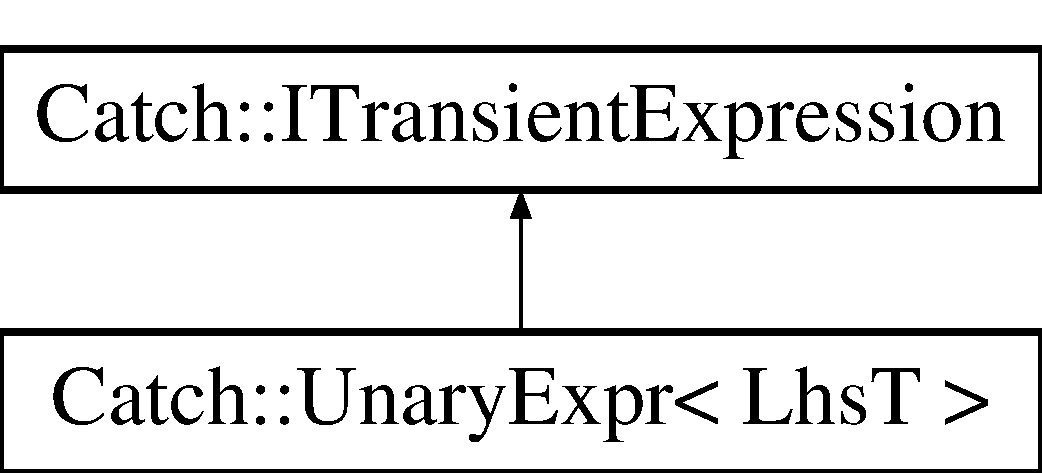
\includegraphics[height=2.000000cm]{class_catch_1_1_unary_expr}
\end{center}
\end{figure}
\subsection*{Public Member Functions}
\begin{DoxyCompactItemize}
\item 
\mbox{\hyperlink{class_catch_1_1_unary_expr_ae02f666a1e64da728628aa2033e1d6e7}{Unary\+Expr}} (LhsT lhs)
\end{DoxyCompactItemize}
\subsection*{Additional Inherited Members}


\subsection{Detailed Description}
\subsubsection*{template$<$typename LhsT$>$\newline
class Catch\+::\+Unary\+Expr$<$ Lhs\+T $>$}



Definition at line 1297 of file catch.\+hpp.



\subsection{Constructor \& Destructor Documentation}
\mbox{\Hypertarget{class_catch_1_1_unary_expr_ae02f666a1e64da728628aa2033e1d6e7}\label{class_catch_1_1_unary_expr_ae02f666a1e64da728628aa2033e1d6e7}} 
\index{Catch\+::\+Unary\+Expr@{Catch\+::\+Unary\+Expr}!Unary\+Expr@{Unary\+Expr}}
\index{Unary\+Expr@{Unary\+Expr}!Catch\+::\+Unary\+Expr@{Catch\+::\+Unary\+Expr}}
\subsubsection{\texorpdfstring{Unary\+Expr()}{UnaryExpr()}}
{\footnotesize\ttfamily template$<$typename LhsT $>$ \\
\mbox{\hyperlink{class_catch_1_1_unary_expr}{Catch\+::\+Unary\+Expr}}$<$ LhsT $>$\+::\mbox{\hyperlink{class_catch_1_1_unary_expr}{Unary\+Expr}} (\begin{DoxyParamCaption}\item[{LhsT}]{lhs }\end{DoxyParamCaption})\hspace{0.3cm}{\ttfamily [inline]}, {\ttfamily [explicit]}}



Definition at line 1305 of file catch.\+hpp.



The documentation for this class was generated from the following file\+:\begin{DoxyCompactItemize}
\item 
D\+:/c++/block\+\_\+matrix-\/master/block\+\_\+matrix-\/master/test/\mbox{\hyperlink{catch_8hpp}{catch.\+hpp}}\end{DoxyCompactItemize}

\hypertarget{struct_catch_1_1_matchers_1_1_vector_1_1_unordered_equals_matcher}{}\section{Catch\+:\+:Matchers\+:\+:Vector\+:\+:Unordered\+Equals\+Matcher$<$ T $>$ Struct Template Reference}
\label{struct_catch_1_1_matchers_1_1_vector_1_1_unordered_equals_matcher}\index{Catch\+::\+Matchers\+::\+Vector\+::\+Unordered\+Equals\+Matcher$<$ T $>$@{Catch\+::\+Matchers\+::\+Vector\+::\+Unordered\+Equals\+Matcher$<$ T $>$}}


{\ttfamily \#include $<$catch.\+hpp$>$}

Inheritance diagram for Catch\+:\+:Matchers\+:\+:Vector\+:\+:Unordered\+Equals\+Matcher$<$ T $>$\+:\begin{figure}[H]
\begin{center}
\leavevmode
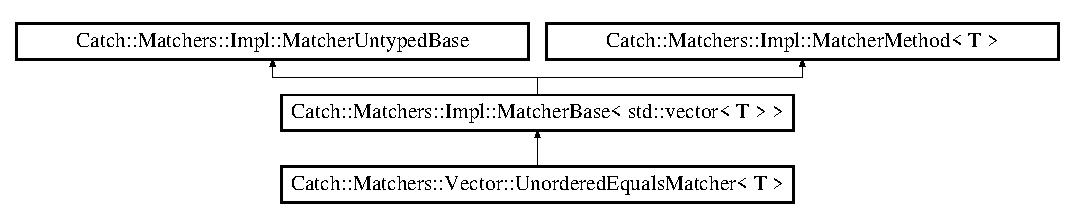
\includegraphics[height=2.492581cm]{struct_catch_1_1_matchers_1_1_vector_1_1_unordered_equals_matcher}
\end{center}
\end{figure}
\subsection*{Public Member Functions}
\begin{DoxyCompactItemize}
\item 
\mbox{\hyperlink{struct_catch_1_1_matchers_1_1_vector_1_1_unordered_equals_matcher_a525905639b2b15b52ddb0bf14bfa19da}{Unordered\+Equals\+Matcher}} (std\+::vector$<$ T $>$ const \&target)
\item 
bool \mbox{\hyperlink{struct_catch_1_1_matchers_1_1_vector_1_1_unordered_equals_matcher_a3ccdd9dd2cd8bdbb8bb121acbb9cb358}{match}} (std\+::vector$<$ T $>$ const \&vec) const override
\item 
std\+::string \mbox{\hyperlink{struct_catch_1_1_matchers_1_1_vector_1_1_unordered_equals_matcher_a7202d811200317abc58c844f663823df}{describe}} () const override
\end{DoxyCompactItemize}
\subsection*{Additional Inherited Members}


\subsection{Detailed Description}
\subsubsection*{template$<$typename T$>$\newline
struct Catch\+::\+Matchers\+::\+Vector\+::\+Unordered\+Equals\+Matcher$<$ T $>$}



Definition at line 2534 of file catch.\+hpp.



\subsection{Constructor \& Destructor Documentation}
\mbox{\Hypertarget{struct_catch_1_1_matchers_1_1_vector_1_1_unordered_equals_matcher_a525905639b2b15b52ddb0bf14bfa19da}\label{struct_catch_1_1_matchers_1_1_vector_1_1_unordered_equals_matcher_a525905639b2b15b52ddb0bf14bfa19da}} 
\index{Catch\+::\+Matchers\+::\+Vector\+::\+Unordered\+Equals\+Matcher@{Catch\+::\+Matchers\+::\+Vector\+::\+Unordered\+Equals\+Matcher}!Unordered\+Equals\+Matcher@{Unordered\+Equals\+Matcher}}
\index{Unordered\+Equals\+Matcher@{Unordered\+Equals\+Matcher}!Catch\+::\+Matchers\+::\+Vector\+::\+Unordered\+Equals\+Matcher@{Catch\+::\+Matchers\+::\+Vector\+::\+Unordered\+Equals\+Matcher}}
\subsubsection{\texorpdfstring{Unordered\+Equals\+Matcher()}{UnorderedEqualsMatcher()}}
{\footnotesize\ttfamily template$<$typename T $>$ \\
\mbox{\hyperlink{struct_catch_1_1_matchers_1_1_vector_1_1_unordered_equals_matcher}{Catch\+::\+Matchers\+::\+Vector\+::\+Unordered\+Equals\+Matcher}}$<$ T $>$\+::\mbox{\hyperlink{struct_catch_1_1_matchers_1_1_vector_1_1_unordered_equals_matcher}{Unordered\+Equals\+Matcher}} (\begin{DoxyParamCaption}\item[{std\+::vector$<$ T $>$ const \&}]{target }\end{DoxyParamCaption})\hspace{0.3cm}{\ttfamily [inline]}}



Definition at line 2535 of file catch.\+hpp.



\subsection{Member Function Documentation}
\mbox{\Hypertarget{struct_catch_1_1_matchers_1_1_vector_1_1_unordered_equals_matcher_a7202d811200317abc58c844f663823df}\label{struct_catch_1_1_matchers_1_1_vector_1_1_unordered_equals_matcher_a7202d811200317abc58c844f663823df}} 
\index{Catch\+::\+Matchers\+::\+Vector\+::\+Unordered\+Equals\+Matcher@{Catch\+::\+Matchers\+::\+Vector\+::\+Unordered\+Equals\+Matcher}!describe@{describe}}
\index{describe@{describe}!Catch\+::\+Matchers\+::\+Vector\+::\+Unordered\+Equals\+Matcher@{Catch\+::\+Matchers\+::\+Vector\+::\+Unordered\+Equals\+Matcher}}
\subsubsection{\texorpdfstring{describe()}{describe()}}
{\footnotesize\ttfamily template$<$typename T $>$ \\
std\+::string \mbox{\hyperlink{struct_catch_1_1_matchers_1_1_vector_1_1_unordered_equals_matcher}{Catch\+::\+Matchers\+::\+Vector\+::\+Unordered\+Equals\+Matcher}}$<$ T $>$\+::describe (\begin{DoxyParamCaption}{ }\end{DoxyParamCaption}) const\hspace{0.3cm}{\ttfamily [inline]}, {\ttfamily [override]}, {\ttfamily [virtual]}}



Implements \mbox{\hyperlink{class_catch_1_1_matchers_1_1_impl_1_1_matcher_untyped_base_a91d3a907dbfcbb596077df24f6e11fe2}{Catch\+::\+Matchers\+::\+Impl\+::\+Matcher\+Untyped\+Base}}.



Definition at line 2566 of file catch.\+hpp.

\mbox{\Hypertarget{struct_catch_1_1_matchers_1_1_vector_1_1_unordered_equals_matcher_a3ccdd9dd2cd8bdbb8bb121acbb9cb358}\label{struct_catch_1_1_matchers_1_1_vector_1_1_unordered_equals_matcher_a3ccdd9dd2cd8bdbb8bb121acbb9cb358}} 
\index{Catch\+::\+Matchers\+::\+Vector\+::\+Unordered\+Equals\+Matcher@{Catch\+::\+Matchers\+::\+Vector\+::\+Unordered\+Equals\+Matcher}!match@{match}}
\index{match@{match}!Catch\+::\+Matchers\+::\+Vector\+::\+Unordered\+Equals\+Matcher@{Catch\+::\+Matchers\+::\+Vector\+::\+Unordered\+Equals\+Matcher}}
\subsubsection{\texorpdfstring{match()}{match()}}
{\footnotesize\ttfamily template$<$typename T $>$ \\
bool \mbox{\hyperlink{struct_catch_1_1_matchers_1_1_vector_1_1_unordered_equals_matcher}{Catch\+::\+Matchers\+::\+Vector\+::\+Unordered\+Equals\+Matcher}}$<$ T $>$\+::match (\begin{DoxyParamCaption}\item[{std\+::vector$<$ T $>$ const \&}]{vec }\end{DoxyParamCaption}) const\hspace{0.3cm}{\ttfamily [inline]}, {\ttfamily [override]}}



Definition at line 2536 of file catch.\+hpp.



The documentation for this struct was generated from the following file\+:\begin{DoxyCompactItemize}
\item 
D\+:/c++/block\+\_\+matrix-\/master/block\+\_\+matrix-\/master/test/\mbox{\hyperlink{catch_8hpp}{catch.\+hpp}}\end{DoxyCompactItemize}

\hypertarget{struct_catch_1_1_matchers_1_1_floating_1_1_within_abs_matcher}{}\section{Catch\+:\+:Matchers\+:\+:Floating\+:\+:Within\+Abs\+Matcher Struct Reference}
\label{struct_catch_1_1_matchers_1_1_floating_1_1_within_abs_matcher}\index{Catch\+::\+Matchers\+::\+Floating\+::\+Within\+Abs\+Matcher@{Catch\+::\+Matchers\+::\+Floating\+::\+Within\+Abs\+Matcher}}


{\ttfamily \#include $<$catch.\+hpp$>$}

Inheritance diagram for Catch\+:\+:Matchers\+:\+:Floating\+:\+:Within\+Abs\+Matcher\+:\begin{figure}[H]
\begin{center}
\leavevmode
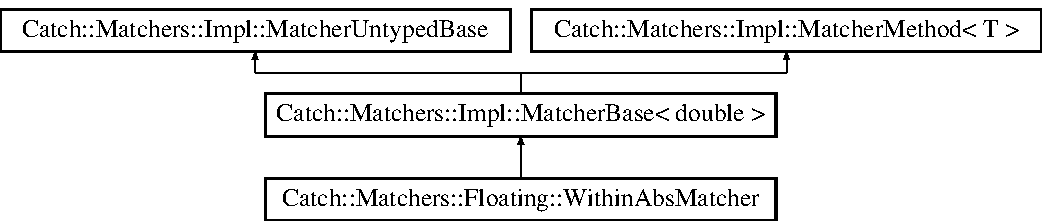
\includegraphics[height=2.968198cm]{struct_catch_1_1_matchers_1_1_floating_1_1_within_abs_matcher}
\end{center}
\end{figure}
\subsection*{Public Member Functions}
\begin{DoxyCompactItemize}
\item 
\mbox{\hyperlink{struct_catch_1_1_matchers_1_1_floating_1_1_within_abs_matcher_ac45340b98c41230a7def5bd86c2d870f}{Within\+Abs\+Matcher}} (double target, double margin)
\item 
bool \mbox{\hyperlink{struct_catch_1_1_matchers_1_1_floating_1_1_within_abs_matcher_afa5d8eed57f12c1e5d006471eb0bfe72}{match}} (double const \&matchee) const override
\item 
std\+::string \mbox{\hyperlink{struct_catch_1_1_matchers_1_1_floating_1_1_within_abs_matcher_a206a738680f8767af31d3f1835afff3f}{describe}} () const override
\end{DoxyCompactItemize}
\subsection*{Additional Inherited Members}


\subsection{Detailed Description}


Definition at line 2329 of file catch.\+hpp.



\subsection{Constructor \& Destructor Documentation}
\mbox{\Hypertarget{struct_catch_1_1_matchers_1_1_floating_1_1_within_abs_matcher_ac45340b98c41230a7def5bd86c2d870f}\label{struct_catch_1_1_matchers_1_1_floating_1_1_within_abs_matcher_ac45340b98c41230a7def5bd86c2d870f}} 
\index{Catch\+::\+Matchers\+::\+Floating\+::\+Within\+Abs\+Matcher@{Catch\+::\+Matchers\+::\+Floating\+::\+Within\+Abs\+Matcher}!Within\+Abs\+Matcher@{Within\+Abs\+Matcher}}
\index{Within\+Abs\+Matcher@{Within\+Abs\+Matcher}!Catch\+::\+Matchers\+::\+Floating\+::\+Within\+Abs\+Matcher@{Catch\+::\+Matchers\+::\+Floating\+::\+Within\+Abs\+Matcher}}
\subsubsection{\texorpdfstring{Within\+Abs\+Matcher()}{WithinAbsMatcher()}}
{\footnotesize\ttfamily Catch\+::\+Matchers\+::\+Floating\+::\+Within\+Abs\+Matcher\+::\+Within\+Abs\+Matcher (\begin{DoxyParamCaption}\item[{double}]{target,  }\item[{double}]{margin }\end{DoxyParamCaption})}



\subsection{Member Function Documentation}
\mbox{\Hypertarget{struct_catch_1_1_matchers_1_1_floating_1_1_within_abs_matcher_a206a738680f8767af31d3f1835afff3f}\label{struct_catch_1_1_matchers_1_1_floating_1_1_within_abs_matcher_a206a738680f8767af31d3f1835afff3f}} 
\index{Catch\+::\+Matchers\+::\+Floating\+::\+Within\+Abs\+Matcher@{Catch\+::\+Matchers\+::\+Floating\+::\+Within\+Abs\+Matcher}!describe@{describe}}
\index{describe@{describe}!Catch\+::\+Matchers\+::\+Floating\+::\+Within\+Abs\+Matcher@{Catch\+::\+Matchers\+::\+Floating\+::\+Within\+Abs\+Matcher}}
\subsubsection{\texorpdfstring{describe()}{describe()}}
{\footnotesize\ttfamily std\+::string Catch\+::\+Matchers\+::\+Floating\+::\+Within\+Abs\+Matcher\+::describe (\begin{DoxyParamCaption}{ }\end{DoxyParamCaption}) const\hspace{0.3cm}{\ttfamily [override]}, {\ttfamily [virtual]}}



Implements \mbox{\hyperlink{class_catch_1_1_matchers_1_1_impl_1_1_matcher_untyped_base_a91d3a907dbfcbb596077df24f6e11fe2}{Catch\+::\+Matchers\+::\+Impl\+::\+Matcher\+Untyped\+Base}}.

\mbox{\Hypertarget{struct_catch_1_1_matchers_1_1_floating_1_1_within_abs_matcher_afa5d8eed57f12c1e5d006471eb0bfe72}\label{struct_catch_1_1_matchers_1_1_floating_1_1_within_abs_matcher_afa5d8eed57f12c1e5d006471eb0bfe72}} 
\index{Catch\+::\+Matchers\+::\+Floating\+::\+Within\+Abs\+Matcher@{Catch\+::\+Matchers\+::\+Floating\+::\+Within\+Abs\+Matcher}!match@{match}}
\index{match@{match}!Catch\+::\+Matchers\+::\+Floating\+::\+Within\+Abs\+Matcher@{Catch\+::\+Matchers\+::\+Floating\+::\+Within\+Abs\+Matcher}}
\subsubsection{\texorpdfstring{match()}{match()}}
{\footnotesize\ttfamily bool Catch\+::\+Matchers\+::\+Floating\+::\+Within\+Abs\+Matcher\+::match (\begin{DoxyParamCaption}\item[{double const \&}]{matchee }\end{DoxyParamCaption}) const\hspace{0.3cm}{\ttfamily [override]}}



The documentation for this struct was generated from the following file\+:\begin{DoxyCompactItemize}
\item 
D\+:/c++/block\+\_\+matrix-\/master/block\+\_\+matrix-\/master/test/\mbox{\hyperlink{catch_8hpp}{catch.\+hpp}}\end{DoxyCompactItemize}

\hypertarget{struct_catch_1_1_matchers_1_1_floating_1_1_within_ulps_matcher}{}\section{Catch\+:\+:Matchers\+:\+:Floating\+:\+:Within\+Ulps\+Matcher Struct Reference}
\label{struct_catch_1_1_matchers_1_1_floating_1_1_within_ulps_matcher}\index{Catch\+::\+Matchers\+::\+Floating\+::\+Within\+Ulps\+Matcher@{Catch\+::\+Matchers\+::\+Floating\+::\+Within\+Ulps\+Matcher}}


{\ttfamily \#include $<$catch.\+hpp$>$}

Inheritance diagram for Catch\+:\+:Matchers\+:\+:Floating\+:\+:Within\+Ulps\+Matcher\+:\begin{figure}[H]
\begin{center}
\leavevmode
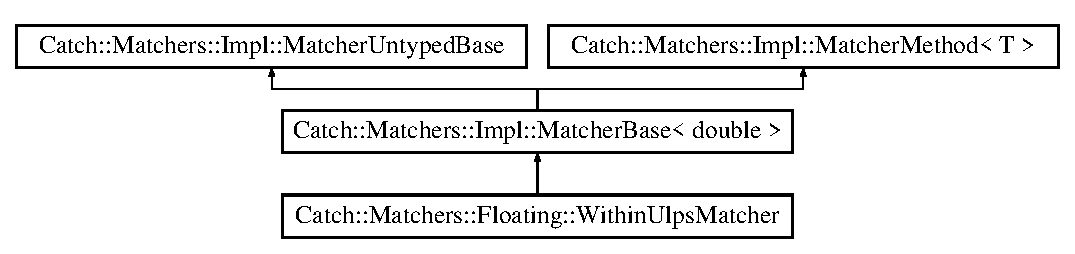
\includegraphics[height=2.968198cm]{struct_catch_1_1_matchers_1_1_floating_1_1_within_ulps_matcher}
\end{center}
\end{figure}
\subsection*{Public Member Functions}
\begin{DoxyCompactItemize}
\item 
\mbox{\hyperlink{struct_catch_1_1_matchers_1_1_floating_1_1_within_ulps_matcher_a836074ae4010275284ab66b2485c6575}{Within\+Ulps\+Matcher}} (double target, int ulps, Floating\+Point\+Kind base\+Type)
\item 
bool \mbox{\hyperlink{struct_catch_1_1_matchers_1_1_floating_1_1_within_ulps_matcher_aabda42a0dc5d00f3c5916feb75006b32}{match}} (double const \&matchee) const override
\item 
std\+::string \mbox{\hyperlink{struct_catch_1_1_matchers_1_1_floating_1_1_within_ulps_matcher_ad9bc8bb7f3abd326580a4bf6cf369b1b}{describe}} () const override
\end{DoxyCompactItemize}
\subsection*{Additional Inherited Members}


\subsection{Detailed Description}


Definition at line 2338 of file catch.\+hpp.



\subsection{Constructor \& Destructor Documentation}
\mbox{\Hypertarget{struct_catch_1_1_matchers_1_1_floating_1_1_within_ulps_matcher_a836074ae4010275284ab66b2485c6575}\label{struct_catch_1_1_matchers_1_1_floating_1_1_within_ulps_matcher_a836074ae4010275284ab66b2485c6575}} 
\index{Catch\+::\+Matchers\+::\+Floating\+::\+Within\+Ulps\+Matcher@{Catch\+::\+Matchers\+::\+Floating\+::\+Within\+Ulps\+Matcher}!Within\+Ulps\+Matcher@{Within\+Ulps\+Matcher}}
\index{Within\+Ulps\+Matcher@{Within\+Ulps\+Matcher}!Catch\+::\+Matchers\+::\+Floating\+::\+Within\+Ulps\+Matcher@{Catch\+::\+Matchers\+::\+Floating\+::\+Within\+Ulps\+Matcher}}
\subsubsection{\texorpdfstring{Within\+Ulps\+Matcher()}{WithinUlpsMatcher()}}
{\footnotesize\ttfamily Catch\+::\+Matchers\+::\+Floating\+::\+Within\+Ulps\+Matcher\+::\+Within\+Ulps\+Matcher (\begin{DoxyParamCaption}\item[{double}]{target,  }\item[{int}]{ulps,  }\item[{Floating\+Point\+Kind}]{base\+Type }\end{DoxyParamCaption})}



\subsection{Member Function Documentation}
\mbox{\Hypertarget{struct_catch_1_1_matchers_1_1_floating_1_1_within_ulps_matcher_ad9bc8bb7f3abd326580a4bf6cf369b1b}\label{struct_catch_1_1_matchers_1_1_floating_1_1_within_ulps_matcher_ad9bc8bb7f3abd326580a4bf6cf369b1b}} 
\index{Catch\+::\+Matchers\+::\+Floating\+::\+Within\+Ulps\+Matcher@{Catch\+::\+Matchers\+::\+Floating\+::\+Within\+Ulps\+Matcher}!describe@{describe}}
\index{describe@{describe}!Catch\+::\+Matchers\+::\+Floating\+::\+Within\+Ulps\+Matcher@{Catch\+::\+Matchers\+::\+Floating\+::\+Within\+Ulps\+Matcher}}
\subsubsection{\texorpdfstring{describe()}{describe()}}
{\footnotesize\ttfamily std\+::string Catch\+::\+Matchers\+::\+Floating\+::\+Within\+Ulps\+Matcher\+::describe (\begin{DoxyParamCaption}{ }\end{DoxyParamCaption}) const\hspace{0.3cm}{\ttfamily [override]}, {\ttfamily [virtual]}}



Implements \mbox{\hyperlink{class_catch_1_1_matchers_1_1_impl_1_1_matcher_untyped_base_a91d3a907dbfcbb596077df24f6e11fe2}{Catch\+::\+Matchers\+::\+Impl\+::\+Matcher\+Untyped\+Base}}.

\mbox{\Hypertarget{struct_catch_1_1_matchers_1_1_floating_1_1_within_ulps_matcher_aabda42a0dc5d00f3c5916feb75006b32}\label{struct_catch_1_1_matchers_1_1_floating_1_1_within_ulps_matcher_aabda42a0dc5d00f3c5916feb75006b32}} 
\index{Catch\+::\+Matchers\+::\+Floating\+::\+Within\+Ulps\+Matcher@{Catch\+::\+Matchers\+::\+Floating\+::\+Within\+Ulps\+Matcher}!match@{match}}
\index{match@{match}!Catch\+::\+Matchers\+::\+Floating\+::\+Within\+Ulps\+Matcher@{Catch\+::\+Matchers\+::\+Floating\+::\+Within\+Ulps\+Matcher}}
\subsubsection{\texorpdfstring{match()}{match()}}
{\footnotesize\ttfamily bool Catch\+::\+Matchers\+::\+Floating\+::\+Within\+Ulps\+Matcher\+::match (\begin{DoxyParamCaption}\item[{double const \&}]{matchee }\end{DoxyParamCaption}) const\hspace{0.3cm}{\ttfamily [override]}}



The documentation for this struct was generated from the following file\+:\begin{DoxyCompactItemize}
\item 
D\+:/c++/block\+\_\+matrix-\/master/block\+\_\+matrix-\/master/test/\mbox{\hyperlink{catch_8hpp}{catch.\+hpp}}\end{DoxyCompactItemize}

\chapter{File Documentation}
\hypertarget{include_2block__matrix_8hpp}{}\section{D\+:/c++/block\+\_\+matrix-\/master/block\+\_\+matrix-\/master/include/block\+\_\+matrix.hpp File Reference}
\label{include_2block__matrix_8hpp}\index{D\+:/c++/block\+\_\+matrix-\/master/block\+\_\+matrix-\/master/include/block\+\_\+matrix.\+hpp@{D\+:/c++/block\+\_\+matrix-\/master/block\+\_\+matrix-\/master/include/block\+\_\+matrix.\+hpp}}
{\ttfamily \#include $<$vector$>$}\newline
{\ttfamily \#include $<$iostream$>$}\newline
{\ttfamily \#include \char`\"{}exception\+\_\+handling.\+hpp\char`\"{}}\newline

\hypertarget{test_2include_2block__matrix_8hpp}{}\section{D\+:/c++/block\+\_\+matrix-\/master/block\+\_\+matrix-\/master/test/include/block\+\_\+matrix.hpp File Reference}
\label{test_2include_2block__matrix_8hpp}\index{D\+:/c++/block\+\_\+matrix-\/master/block\+\_\+matrix-\/master/test/include/block\+\_\+matrix.\+hpp@{D\+:/c++/block\+\_\+matrix-\/master/block\+\_\+matrix-\/master/test/include/block\+\_\+matrix.\+hpp}}
{\ttfamily \#include $<$vector$>$}\newline
{\ttfamily \#include $<$iostream$>$}\newline
{\ttfamily \#include \char`\"{}exception\+\_\+handling.\+hpp\char`\"{}}\newline
\subsection*{Classes}
\begin{DoxyCompactItemize}
\item 
class \mbox{\hyperlink{classbmx_1_1block__matrix}{bmx\+::block\+\_\+matrix$<$ Type $>$}}
\end{DoxyCompactItemize}
\subsection*{Namespaces}
\begin{DoxyCompactItemize}
\item 
 \mbox{\hyperlink{namespacebmx}{bmx}}
\end{DoxyCompactItemize}

\hypertarget{include_2exception__handling_8hpp}{}\section{D\+:/c++/block\+\_\+matrix-\/master/block\+\_\+matrix-\/master/include/exception\+\_\+handling.hpp File Reference}
\label{include_2exception__handling_8hpp}\index{D\+:/c++/block\+\_\+matrix-\/master/block\+\_\+matrix-\/master/include/exception\+\_\+handling.\+hpp@{D\+:/c++/block\+\_\+matrix-\/master/block\+\_\+matrix-\/master/include/exception\+\_\+handling.\+hpp}}
{\ttfamily \#include $<$stdexcept$>$}\newline
{\ttfamily \#include \char`\"{}block\+\_\+matrix.\+hpp\char`\"{}}\newline
\subsection*{Classes}
\begin{DoxyCompactItemize}
\item 
class \mbox{\hyperlink{classexception_1_1invalid__argument}{exception\+::invalid\+\_\+argument}}
\item 
class \mbox{\hyperlink{classexception_1_1invalid__index}{exception\+::invalid\+\_\+index}}
\item 
class \mbox{\hyperlink{classexception_1_1invalid__matrix}{exception\+::invalid\+\_\+matrix}}
\item 
class \mbox{\hyperlink{classexception_1_1invalid__size}{exception\+::invalid\+\_\+size}}
\end{DoxyCompactItemize}
\subsection*{Namespaces}
\begin{DoxyCompactItemize}
\item 
 \mbox{\hyperlink{namespaceexception}{exception}}
\end{DoxyCompactItemize}

\hypertarget{test_2include_2exception__handling_8hpp}{}\section{D\+:/c++/block\+\_\+matrix-\/master/block\+\_\+matrix-\/master/test/include/exception\+\_\+handling.hpp File Reference}
\label{test_2include_2exception__handling_8hpp}\index{D\+:/c++/block\+\_\+matrix-\/master/block\+\_\+matrix-\/master/test/include/exception\+\_\+handling.\+hpp@{D\+:/c++/block\+\_\+matrix-\/master/block\+\_\+matrix-\/master/test/include/exception\+\_\+handling.\+hpp}}
{\ttfamily \#include $<$stdexcept$>$}\newline
{\ttfamily \#include \char`\"{}block\+\_\+matrix.\+hpp\char`\"{}}\newline
\subsection*{Classes}
\begin{DoxyCompactItemize}
\item 
class \mbox{\hyperlink{classexception_1_1invalid__argument}{exception\+::invalid\+\_\+argument}}
\item 
class \mbox{\hyperlink{classexception_1_1invalid__index}{exception\+::invalid\+\_\+index}}
\item 
class \mbox{\hyperlink{classexception_1_1invalid__matrix}{exception\+::invalid\+\_\+matrix}}
\item 
class \mbox{\hyperlink{classexception_1_1invalid__size}{exception\+::invalid\+\_\+size}}
\end{DoxyCompactItemize}
\subsection*{Namespaces}
\begin{DoxyCompactItemize}
\item 
 \mbox{\hyperlink{namespaceexception}{exception}}
\end{DoxyCompactItemize}

\hypertarget{include_2menu_8hpp}{}\section{D\+:/c++/block\+\_\+matrix-\/master/block\+\_\+matrix-\/master/include/menu.hpp File Reference}
\label{include_2menu_8hpp}\index{D\+:/c++/block\+\_\+matrix-\/master/block\+\_\+matrix-\/master/include/menu.\+hpp@{D\+:/c++/block\+\_\+matrix-\/master/block\+\_\+matrix-\/master/include/menu.\+hpp}}
{\ttfamily \#include $<$iostream$>$}\newline
{\ttfamily \#include \char`\"{}exception\+\_\+handling.\+hpp\char`\"{}}\newline
{\ttfamily \#include \char`\"{}block\+\_\+matrix.\+hpp\char`\"{}}\newline
\subsection*{Functions}
\begin{DoxyCompactItemize}
\item 
void \mbox{\hyperlink{include_2menu_8hpp_acee3008b1b6d201023f17979a8099833}{make\+\_\+new\+\_\+bm}} ()
\item 
void \mbox{\hyperlink{include_2menu_8hpp_aa81a6ddb512ea34662307a1ea864a6f0}{sum\+\_\+two\+\_\+bm}} ()
\item 
void \mbox{\hyperlink{include_2menu_8hpp_a6cddd2e653e21c220eede3271f42354f}{multi\+\_\+two\+\_\+bm}} ()
\item 
void \mbox{\hyperlink{include_2menu_8hpp_a64784cd3d9be9bffa60caaf7c6dd1b96}{print\+\_\+matrix}} ()
\item 
void \mbox{\hyperlink{include_2menu_8hpp_a4a3e8f82db9b5dd5037fceb234829ea8}{get\+\_\+element}} ()
\item 
int \mbox{\hyperlink{include_2menu_8hpp_ae83fcdbeb2b6757fc741ae953b633ee1}{menu}} ()
\item 
void \mbox{\hyperlink{include_2menu_8hpp_a5173d91734aa49f37755070894ace2b7}{progress}} (int c)
\end{DoxyCompactItemize}
\subsection*{Variables}
\begin{DoxyCompactItemize}
\item 
\mbox{\hyperlink{classbmx_1_1block__matrix}{bmx\+::block\+\_\+matrix}}$<$ int $>$ \mbox{\hyperlink{include_2menu_8hpp_a775dd4bd250d6f6946b71307e0c5de9a}{bm\+\_\+one}}
\item 
\mbox{\hyperlink{classbmx_1_1block__matrix}{bmx\+::block\+\_\+matrix}}$<$ int $>$ \mbox{\hyperlink{include_2menu_8hpp_a15a653414a37d01b74d6339eb480071b}{bm\+\_\+two}}
\item 
bool \mbox{\hyperlink{include_2menu_8hpp_a6b30e391e4d5b2b4d40e712718287013}{is\+\_\+exist}} = false
\end{DoxyCompactItemize}


\subsection{Function Documentation}
\mbox{\Hypertarget{include_2menu_8hpp_a4a3e8f82db9b5dd5037fceb234829ea8}\label{include_2menu_8hpp_a4a3e8f82db9b5dd5037fceb234829ea8}} 
\index{include/menu.\+hpp@{include/menu.\+hpp}!get\+\_\+element@{get\+\_\+element}}
\index{get\+\_\+element@{get\+\_\+element}!include/menu.\+hpp@{include/menu.\+hpp}}
\subsubsection{\texorpdfstring{get\+\_\+element()}{get\_element()}}
{\footnotesize\ttfamily void get\+\_\+element (\begin{DoxyParamCaption}{ }\end{DoxyParamCaption})}



Definition at line 66 of file menu.\+hpp.

\mbox{\Hypertarget{include_2menu_8hpp_acee3008b1b6d201023f17979a8099833}\label{include_2menu_8hpp_acee3008b1b6d201023f17979a8099833}} 
\index{include/menu.\+hpp@{include/menu.\+hpp}!make\+\_\+new\+\_\+bm@{make\+\_\+new\+\_\+bm}}
\index{make\+\_\+new\+\_\+bm@{make\+\_\+new\+\_\+bm}!include/menu.\+hpp@{include/menu.\+hpp}}
\subsubsection{\texorpdfstring{make\+\_\+new\+\_\+bm()}{make\_new\_bm()}}
{\footnotesize\ttfamily void make\+\_\+new\+\_\+bm (\begin{DoxyParamCaption}{ }\end{DoxyParamCaption})}



Definition at line 13 of file menu.\+hpp.

\mbox{\Hypertarget{include_2menu_8hpp_ae83fcdbeb2b6757fc741ae953b633ee1}\label{include_2menu_8hpp_ae83fcdbeb2b6757fc741ae953b633ee1}} 
\index{include/menu.\+hpp@{include/menu.\+hpp}!menu@{menu}}
\index{menu@{menu}!include/menu.\+hpp@{include/menu.\+hpp}}
\subsubsection{\texorpdfstring{menu()}{menu()}}
{\footnotesize\ttfamily int menu (\begin{DoxyParamCaption}{ }\end{DoxyParamCaption})}



Definition at line 79 of file menu.\+hpp.

\mbox{\Hypertarget{include_2menu_8hpp_a6cddd2e653e21c220eede3271f42354f}\label{include_2menu_8hpp_a6cddd2e653e21c220eede3271f42354f}} 
\index{include/menu.\+hpp@{include/menu.\+hpp}!multi\+\_\+two\+\_\+bm@{multi\+\_\+two\+\_\+bm}}
\index{multi\+\_\+two\+\_\+bm@{multi\+\_\+two\+\_\+bm}!include/menu.\+hpp@{include/menu.\+hpp}}
\subsubsection{\texorpdfstring{multi\+\_\+two\+\_\+bm()}{multi\_two\_bm()}}
{\footnotesize\ttfamily void multi\+\_\+two\+\_\+bm (\begin{DoxyParamCaption}{ }\end{DoxyParamCaption})}



Definition at line 41 of file menu.\+hpp.

\mbox{\Hypertarget{include_2menu_8hpp_a64784cd3d9be9bffa60caaf7c6dd1b96}\label{include_2menu_8hpp_a64784cd3d9be9bffa60caaf7c6dd1b96}} 
\index{include/menu.\+hpp@{include/menu.\+hpp}!print\+\_\+matrix@{print\+\_\+matrix}}
\index{print\+\_\+matrix@{print\+\_\+matrix}!include/menu.\+hpp@{include/menu.\+hpp}}
\subsubsection{\texorpdfstring{print\+\_\+matrix()}{print\_matrix()}}
{\footnotesize\ttfamily void print\+\_\+matrix (\begin{DoxyParamCaption}{ }\end{DoxyParamCaption})}



Definition at line 56 of file menu.\+hpp.

\mbox{\Hypertarget{include_2menu_8hpp_a5173d91734aa49f37755070894ace2b7}\label{include_2menu_8hpp_a5173d91734aa49f37755070894ace2b7}} 
\index{include/menu.\+hpp@{include/menu.\+hpp}!progress@{progress}}
\index{progress@{progress}!include/menu.\+hpp@{include/menu.\+hpp}}
\subsubsection{\texorpdfstring{progress()}{progress()}}
{\footnotesize\ttfamily void progress (\begin{DoxyParamCaption}\item[{int}]{c }\end{DoxyParamCaption})}



Definition at line 101 of file menu.\+hpp.

\mbox{\Hypertarget{include_2menu_8hpp_aa81a6ddb512ea34662307a1ea864a6f0}\label{include_2menu_8hpp_aa81a6ddb512ea34662307a1ea864a6f0}} 
\index{include/menu.\+hpp@{include/menu.\+hpp}!sum\+\_\+two\+\_\+bm@{sum\+\_\+two\+\_\+bm}}
\index{sum\+\_\+two\+\_\+bm@{sum\+\_\+two\+\_\+bm}!include/menu.\+hpp@{include/menu.\+hpp}}
\subsubsection{\texorpdfstring{sum\+\_\+two\+\_\+bm()}{sum\_two\_bm()}}
{\footnotesize\ttfamily void sum\+\_\+two\+\_\+bm (\begin{DoxyParamCaption}{ }\end{DoxyParamCaption})}



Definition at line 24 of file menu.\+hpp.



\subsection{Variable Documentation}
\mbox{\Hypertarget{include_2menu_8hpp_a775dd4bd250d6f6946b71307e0c5de9a}\label{include_2menu_8hpp_a775dd4bd250d6f6946b71307e0c5de9a}} 
\index{include/menu.\+hpp@{include/menu.\+hpp}!bm\+\_\+one@{bm\+\_\+one}}
\index{bm\+\_\+one@{bm\+\_\+one}!include/menu.\+hpp@{include/menu.\+hpp}}
\subsubsection{\texorpdfstring{bm\+\_\+one}{bm\_one}}
{\footnotesize\ttfamily \mbox{\hyperlink{classbmx_1_1block__matrix}{bmx\+::block\+\_\+matrix}}$<$int$>$ bm\+\_\+one}



Definition at line 9 of file menu.\+hpp.

\mbox{\Hypertarget{include_2menu_8hpp_a15a653414a37d01b74d6339eb480071b}\label{include_2menu_8hpp_a15a653414a37d01b74d6339eb480071b}} 
\index{include/menu.\+hpp@{include/menu.\+hpp}!bm\+\_\+two@{bm\+\_\+two}}
\index{bm\+\_\+two@{bm\+\_\+two}!include/menu.\+hpp@{include/menu.\+hpp}}
\subsubsection{\texorpdfstring{bm\+\_\+two}{bm\_two}}
{\footnotesize\ttfamily \mbox{\hyperlink{classbmx_1_1block__matrix}{bmx\+::block\+\_\+matrix}}$<$int$>$ bm\+\_\+two}



Definition at line 10 of file menu.\+hpp.

\mbox{\Hypertarget{include_2menu_8hpp_a6b30e391e4d5b2b4d40e712718287013}\label{include_2menu_8hpp_a6b30e391e4d5b2b4d40e712718287013}} 
\index{include/menu.\+hpp@{include/menu.\+hpp}!is\+\_\+exist@{is\+\_\+exist}}
\index{is\+\_\+exist@{is\+\_\+exist}!include/menu.\+hpp@{include/menu.\+hpp}}
\subsubsection{\texorpdfstring{is\+\_\+exist}{is\_exist}}
{\footnotesize\ttfamily bool is\+\_\+exist = false}



Definition at line 11 of file menu.\+hpp.


\hypertarget{test_2include_2menu_8hpp}{}\section{D\+:/c++/block\+\_\+matrix-\/master/block\+\_\+matrix-\/master/test/include/menu.hpp File Reference}
\label{test_2include_2menu_8hpp}\index{D\+:/c++/block\+\_\+matrix-\/master/block\+\_\+matrix-\/master/test/include/menu.\+hpp@{D\+:/c++/block\+\_\+matrix-\/master/block\+\_\+matrix-\/master/test/include/menu.\+hpp}}
{\ttfamily \#include $<$iostream$>$}\newline
{\ttfamily \#include \char`\"{}exception\+\_\+handling.\+hpp\char`\"{}}\newline
{\ttfamily \#include \char`\"{}block\+\_\+matrix.\+hpp\char`\"{}}\newline
\subsection*{Functions}
\begin{DoxyCompactItemize}
\item 
void \mbox{\hyperlink{test_2include_2menu_8hpp_acee3008b1b6d201023f17979a8099833}{make\+\_\+new\+\_\+bm}} ()
\item 
void \mbox{\hyperlink{test_2include_2menu_8hpp_aa81a6ddb512ea34662307a1ea864a6f0}{sum\+\_\+two\+\_\+bm}} ()
\item 
void \mbox{\hyperlink{test_2include_2menu_8hpp_a6cddd2e653e21c220eede3271f42354f}{multi\+\_\+two\+\_\+bm}} ()
\item 
void \mbox{\hyperlink{test_2include_2menu_8hpp_a64784cd3d9be9bffa60caaf7c6dd1b96}{print\+\_\+matrix}} ()
\item 
void \mbox{\hyperlink{test_2include_2menu_8hpp_a4a3e8f82db9b5dd5037fceb234829ea8}{get\+\_\+element}} ()
\item 
int \mbox{\hyperlink{test_2include_2menu_8hpp_ae83fcdbeb2b6757fc741ae953b633ee1}{menu}} ()
\item 
void \mbox{\hyperlink{test_2include_2menu_8hpp_a5173d91734aa49f37755070894ace2b7}{progress}} (int c)
\end{DoxyCompactItemize}
\subsection*{Variables}
\begin{DoxyCompactItemize}
\item 
\mbox{\hyperlink{classbmx_1_1block__matrix}{bmx\+::block\+\_\+matrix}}$<$ int $>$ \mbox{\hyperlink{test_2include_2menu_8hpp_a775dd4bd250d6f6946b71307e0c5de9a}{bm\+\_\+one}}
\item 
\mbox{\hyperlink{classbmx_1_1block__matrix}{bmx\+::block\+\_\+matrix}}$<$ int $>$ \mbox{\hyperlink{test_2include_2menu_8hpp_a15a653414a37d01b74d6339eb480071b}{bm\+\_\+two}}
\end{DoxyCompactItemize}


\subsection{Function Documentation}
\mbox{\Hypertarget{test_2include_2menu_8hpp_a4a3e8f82db9b5dd5037fceb234829ea8}\label{test_2include_2menu_8hpp_a4a3e8f82db9b5dd5037fceb234829ea8}} 
\index{test/include/menu.\+hpp@{test/include/menu.\+hpp}!get\+\_\+element@{get\+\_\+element}}
\index{get\+\_\+element@{get\+\_\+element}!test/include/menu.\+hpp@{test/include/menu.\+hpp}}
\subsubsection{\texorpdfstring{get\+\_\+element()}{get\_element()}}
{\footnotesize\ttfamily void get\+\_\+element (\begin{DoxyParamCaption}{ }\end{DoxyParamCaption})}



Definition at line 54 of file menu.\+hpp.

\mbox{\Hypertarget{test_2include_2menu_8hpp_acee3008b1b6d201023f17979a8099833}\label{test_2include_2menu_8hpp_acee3008b1b6d201023f17979a8099833}} 
\index{test/include/menu.\+hpp@{test/include/menu.\+hpp}!make\+\_\+new\+\_\+bm@{make\+\_\+new\+\_\+bm}}
\index{make\+\_\+new\+\_\+bm@{make\+\_\+new\+\_\+bm}!test/include/menu.\+hpp@{test/include/menu.\+hpp}}
\subsubsection{\texorpdfstring{make\+\_\+new\+\_\+bm()}{make\_new\_bm()}}
{\footnotesize\ttfamily void make\+\_\+new\+\_\+bm (\begin{DoxyParamCaption}{ }\end{DoxyParamCaption})}



Definition at line 12 of file menu.\+hpp.

\mbox{\Hypertarget{test_2include_2menu_8hpp_ae83fcdbeb2b6757fc741ae953b633ee1}\label{test_2include_2menu_8hpp_ae83fcdbeb2b6757fc741ae953b633ee1}} 
\index{test/include/menu.\+hpp@{test/include/menu.\+hpp}!menu@{menu}}
\index{menu@{menu}!test/include/menu.\+hpp@{test/include/menu.\+hpp}}
\subsubsection{\texorpdfstring{menu()}{menu()}}
{\footnotesize\ttfamily int menu (\begin{DoxyParamCaption}{ }\end{DoxyParamCaption})}



Definition at line 71 of file menu.\+hpp.

\mbox{\Hypertarget{test_2include_2menu_8hpp_a6cddd2e653e21c220eede3271f42354f}\label{test_2include_2menu_8hpp_a6cddd2e653e21c220eede3271f42354f}} 
\index{test/include/menu.\+hpp@{test/include/menu.\+hpp}!multi\+\_\+two\+\_\+bm@{multi\+\_\+two\+\_\+bm}}
\index{multi\+\_\+two\+\_\+bm@{multi\+\_\+two\+\_\+bm}!test/include/menu.\+hpp@{test/include/menu.\+hpp}}
\subsubsection{\texorpdfstring{multi\+\_\+two\+\_\+bm()}{multi\_two\_bm()}}
{\footnotesize\ttfamily void multi\+\_\+two\+\_\+bm (\begin{DoxyParamCaption}{ }\end{DoxyParamCaption})}



Definition at line 37 of file menu.\+hpp.

\mbox{\Hypertarget{test_2include_2menu_8hpp_a64784cd3d9be9bffa60caaf7c6dd1b96}\label{test_2include_2menu_8hpp_a64784cd3d9be9bffa60caaf7c6dd1b96}} 
\index{test/include/menu.\+hpp@{test/include/menu.\+hpp}!print\+\_\+matrix@{print\+\_\+matrix}}
\index{print\+\_\+matrix@{print\+\_\+matrix}!test/include/menu.\+hpp@{test/include/menu.\+hpp}}
\subsubsection{\texorpdfstring{print\+\_\+matrix()}{print\_matrix()}}
{\footnotesize\ttfamily void print\+\_\+matrix (\begin{DoxyParamCaption}{ }\end{DoxyParamCaption})}



Definition at line 49 of file menu.\+hpp.

\mbox{\Hypertarget{test_2include_2menu_8hpp_a5173d91734aa49f37755070894ace2b7}\label{test_2include_2menu_8hpp_a5173d91734aa49f37755070894ace2b7}} 
\index{test/include/menu.\+hpp@{test/include/menu.\+hpp}!progress@{progress}}
\index{progress@{progress}!test/include/menu.\+hpp@{test/include/menu.\+hpp}}
\subsubsection{\texorpdfstring{progress()}{progress()}}
{\footnotesize\ttfamily void progress (\begin{DoxyParamCaption}\item[{int}]{c }\end{DoxyParamCaption})}



Definition at line 93 of file menu.\+hpp.

\mbox{\Hypertarget{test_2include_2menu_8hpp_aa81a6ddb512ea34662307a1ea864a6f0}\label{test_2include_2menu_8hpp_aa81a6ddb512ea34662307a1ea864a6f0}} 
\index{test/include/menu.\+hpp@{test/include/menu.\+hpp}!sum\+\_\+two\+\_\+bm@{sum\+\_\+two\+\_\+bm}}
\index{sum\+\_\+two\+\_\+bm@{sum\+\_\+two\+\_\+bm}!test/include/menu.\+hpp@{test/include/menu.\+hpp}}
\subsubsection{\texorpdfstring{sum\+\_\+two\+\_\+bm()}{sum\_two\_bm()}}
{\footnotesize\ttfamily void sum\+\_\+two\+\_\+bm (\begin{DoxyParamCaption}{ }\end{DoxyParamCaption})}



Definition at line 24 of file menu.\+hpp.



\subsection{Variable Documentation}
\mbox{\Hypertarget{test_2include_2menu_8hpp_a775dd4bd250d6f6946b71307e0c5de9a}\label{test_2include_2menu_8hpp_a775dd4bd250d6f6946b71307e0c5de9a}} 
\index{test/include/menu.\+hpp@{test/include/menu.\+hpp}!bm\+\_\+one@{bm\+\_\+one}}
\index{bm\+\_\+one@{bm\+\_\+one}!test/include/menu.\+hpp@{test/include/menu.\+hpp}}
\subsubsection{\texorpdfstring{bm\+\_\+one}{bm\_one}}
{\footnotesize\ttfamily \mbox{\hyperlink{classbmx_1_1block__matrix}{bmx\+::block\+\_\+matrix}}$<$int$>$ bm\+\_\+one}



Definition at line 9 of file menu.\+hpp.

\mbox{\Hypertarget{test_2include_2menu_8hpp_a15a653414a37d01b74d6339eb480071b}\label{test_2include_2menu_8hpp_a15a653414a37d01b74d6339eb480071b}} 
\index{test/include/menu.\+hpp@{test/include/menu.\+hpp}!bm\+\_\+two@{bm\+\_\+two}}
\index{bm\+\_\+two@{bm\+\_\+two}!test/include/menu.\+hpp@{test/include/menu.\+hpp}}
\subsubsection{\texorpdfstring{bm\+\_\+two}{bm\_two}}
{\footnotesize\ttfamily \mbox{\hyperlink{classbmx_1_1block__matrix}{bmx\+::block\+\_\+matrix}}$<$int$>$ bm\+\_\+two}



Definition at line 10 of file menu.\+hpp.


\hypertarget{main_8cpp}{}\section{D\+:/c++/block\+\_\+matrix-\/master/block\+\_\+matrix-\/master/main.cpp File Reference}
\label{main_8cpp}\index{D\+:/c++/block\+\_\+matrix-\/master/block\+\_\+matrix-\/master/main.\+cpp@{D\+:/c++/block\+\_\+matrix-\/master/block\+\_\+matrix-\/master/main.\+cpp}}
{\ttfamily \#include \char`\"{}include/block\+\_\+matrix.\+hpp\char`\"{}}\newline
{\ttfamily \#include \char`\"{}include/exception\+\_\+handling.\+hpp\char`\"{}}\newline
{\ttfamily \#include \char`\"{}include/menu.\+hpp\char`\"{}}\newline
\subsection*{Functions}
\begin{DoxyCompactItemize}
\item 
int \mbox{\hyperlink{main_8cpp_ae66f6b31b5ad750f1fe042a706a4e3d4}{main}} ()
\end{DoxyCompactItemize}


\subsection{Function Documentation}
\mbox{\Hypertarget{main_8cpp_ae66f6b31b5ad750f1fe042a706a4e3d4}\label{main_8cpp_ae66f6b31b5ad750f1fe042a706a4e3d4}} 
\index{main.\+cpp@{main.\+cpp}!main@{main}}
\index{main@{main}!main.\+cpp@{main.\+cpp}}
\subsubsection{\texorpdfstring{main()}{main()}}
{\footnotesize\ttfamily int main (\begin{DoxyParamCaption}{ }\end{DoxyParamCaption})}



Definition at line 5 of file main.\+cpp.


\hypertarget{catch_8hpp}{}\section{D\+:/c++/block\+\_\+matrix-\/master/block\+\_\+matrix-\/master/test/catch.hpp File Reference}
\label{catch_8hpp}\index{D\+:/c++/block\+\_\+matrix-\/master/block\+\_\+matrix-\/master/test/catch.\+hpp@{D\+:/c++/block\+\_\+matrix-\/master/block\+\_\+matrix-\/master/test/catch.\+hpp}}
{\ttfamily \#include $<$iosfwd$>$}\newline
{\ttfamily \#include $<$string$>$}\newline
{\ttfamily \#include $<$cstdint$>$}\newline
{\ttfamily \#include $<$vector$>$}\newline
{\ttfamily \#include $<$memory$>$}\newline
{\ttfamily \#include $<$cstddef$>$}\newline
{\ttfamily \#include $<$type\+\_\+traits$>$}\newline
{\ttfamily \#include $<$ostream$>$}\newline
{\ttfamily \#include $<$exception$>$}\newline
{\ttfamily \#include $<$stdexcept$>$}\newline
{\ttfamily \#include $<$cmath$>$}\newline
{\ttfamily \#include $<$algorithm$>$}\newline
{\ttfamily \#include $<$ctime$>$}\newline
{\ttfamily \#include $<$ratio$>$}\newline
{\ttfamily \#include $<$chrono$>$}\newline
{\ttfamily \#include $<$map$>$}\newline
{\ttfamily \#include $<$set$>$}\newline
{\ttfamily \#include $<$cstring$>$}\newline
{\ttfamily \#include $<$cfloat$>$}\newline
{\ttfamily \#include $<$cstdio$>$}\newline
{\ttfamily \#include $<$assert.\+h$>$}\newline
{\ttfamily \#include $<$limits$>$}\newline
{\ttfamily \#include $<$signal.\+h$>$}\newline
{\ttfamily \#include $<$cassert$>$}\newline
{\ttfamily \#include $<$sstream$>$}\newline
{\ttfamily \#include $<$fstream$>$}\newline
{\ttfamily \#include $<$unistd.\+h$>$}\newline
{\ttfamily \#include $<$cerrno$>$}\newline
{\ttfamily \#include $<$iomanip$>$}\newline
{\ttfamily \#include $<$cstdlib$>$}\newline
{\ttfamily \#include $<$regex$>$}\newline
{\ttfamily \#include $<$ios$>$}\newline
{\ttfamily \#include $<$iostream$>$}\newline
{\ttfamily \#include $<$cctype$>$}\newline
\subsection*{Classes}
\begin{DoxyCompactItemize}
\item 
struct \mbox{\hyperlink{struct_catch_1_1_case_sensitive}{Catch\+::\+Case\+Sensitive}}
\item 
class \mbox{\hyperlink{class_catch_1_1_non_copyable}{Catch\+::\+Non\+Copyable}}
\item 
struct \mbox{\hyperlink{struct_catch_1_1_source_line_info}{Catch\+::\+Source\+Line\+Info}}
\item 
struct \mbox{\hyperlink{struct_catch_1_1_stream_end_stop}{Catch\+::\+Stream\+End\+Stop}}
\item 
struct \mbox{\hyperlink{struct_catch_1_1_registrar_for_tag_aliases}{Catch\+::\+Registrar\+For\+Tag\+Aliases}}
\item 
struct \mbox{\hyperlink{struct_catch_1_1_i_test_invoker}{Catch\+::\+I\+Test\+Invoker}}
\item 
struct \mbox{\hyperlink{struct_catch_1_1_i_test_case_registry}{Catch\+::\+I\+Test\+Case\+Registry}}
\item 
class \mbox{\hyperlink{class_catch_1_1_string_ref}{Catch\+::\+String\+Ref}}
\item 
class \mbox{\hyperlink{class_catch_1_1_test_invoker_as_method}{Catch\+::\+Test\+Invoker\+As\+Method$<$ C $>$}}
\item 
struct \mbox{\hyperlink{struct_catch_1_1_name_and_tags}{Catch\+::\+Name\+And\+Tags}}
\item 
struct \mbox{\hyperlink{struct_catch_1_1_auto_reg}{Catch\+::\+Auto\+Reg}}
\item 
struct \mbox{\hyperlink{struct_catch_1_1_result_was}{Catch\+::\+Result\+Was}}
\item 
struct \mbox{\hyperlink{struct_catch_1_1_result_disposition}{Catch\+::\+Result\+Disposition}}
\item 
struct \mbox{\hyperlink{struct_catch_1_1_assertion_info}{Catch\+::\+Assertion\+Info}}
\item 
struct \mbox{\hyperlink{struct_catch_1_1_i_stream}{Catch\+::\+I\+Stream}}
\item 
class \mbox{\hyperlink{class_catch_1_1_reusable_string_stream}{Catch\+::\+Reusable\+String\+Stream}}
\item 
struct \mbox{\hyperlink{struct_catch__global__namespace__dummy}{Catch\+\_\+global\+\_\+namespace\+\_\+dummy}}
\item 
class \mbox{\hyperlink{class_catch_1_1_detail_1_1_is_stream_insertable}{Catch\+::\+Detail\+::\+Is\+Stream\+Insertable$<$ T $>$}}
\item 
struct \mbox{\hyperlink{struct_catch_1_1_string_maker}{Catch\+::\+String\+Maker$<$ T, typename $>$}}
\item 
struct \mbox{\hyperlink{struct_catch_1_1_string_maker_3_01std_1_1string_01_4}{Catch\+::\+String\+Maker$<$ std\+::string $>$}}
\item 
struct \mbox{\hyperlink{struct_catch_1_1_string_maker_3_01std_1_1wstring_01_4}{Catch\+::\+String\+Maker$<$ std\+::wstring $>$}}
\item 
struct \mbox{\hyperlink{struct_catch_1_1_string_maker_3_01char_01const_01_5_01_4}{Catch\+::\+String\+Maker$<$ char const $\ast$ $>$}}
\item 
struct \mbox{\hyperlink{struct_catch_1_1_string_maker_3_01char_01_5_01_4}{Catch\+::\+String\+Maker$<$ char $\ast$ $>$}}
\item 
struct \mbox{\hyperlink{struct_catch_1_1_string_maker_3_01wchar__t_01const_01_5_01_4}{Catch\+::\+String\+Maker$<$ wchar\+\_\+t const $\ast$ $>$}}
\item 
struct \mbox{\hyperlink{struct_catch_1_1_string_maker_3_01wchar__t_01_5_01_4}{Catch\+::\+String\+Maker$<$ wchar\+\_\+t $\ast$ $>$}}
\item 
struct \mbox{\hyperlink{struct_catch_1_1_string_maker_3_01char[_s_z]_4}{Catch\+::\+String\+Maker$<$ char\mbox{[}\+S\+Z\mbox{]}$>$}}
\item 
struct \mbox{\hyperlink{struct_catch_1_1_string_maker_3_01signed_01char[_s_z]_4}{Catch\+::\+String\+Maker$<$ signed char\mbox{[}\+S\+Z\mbox{]}$>$}}
\item 
struct \mbox{\hyperlink{struct_catch_1_1_string_maker_3_01unsigned_01char[_s_z]_4}{Catch\+::\+String\+Maker$<$ unsigned char\mbox{[}\+S\+Z\mbox{]}$>$}}
\item 
struct \mbox{\hyperlink{struct_catch_1_1_string_maker_3_01int_01_4}{Catch\+::\+String\+Maker$<$ int $>$}}
\item 
struct \mbox{\hyperlink{struct_catch_1_1_string_maker_3_01long_01_4}{Catch\+::\+String\+Maker$<$ long $>$}}
\item 
struct \mbox{\hyperlink{struct_catch_1_1_string_maker_3_01long_01long_01_4}{Catch\+::\+String\+Maker$<$ long long $>$}}
\item 
struct \mbox{\hyperlink{struct_catch_1_1_string_maker_3_01unsigned_01int_01_4}{Catch\+::\+String\+Maker$<$ unsigned int $>$}}
\item 
struct \mbox{\hyperlink{struct_catch_1_1_string_maker_3_01unsigned_01long_01_4}{Catch\+::\+String\+Maker$<$ unsigned long $>$}}
\item 
struct \mbox{\hyperlink{struct_catch_1_1_string_maker_3_01unsigned_01long_01long_01_4}{Catch\+::\+String\+Maker$<$ unsigned long long $>$}}
\item 
struct \mbox{\hyperlink{struct_catch_1_1_string_maker_3_01bool_01_4}{Catch\+::\+String\+Maker$<$ bool $>$}}
\item 
struct \mbox{\hyperlink{struct_catch_1_1_string_maker_3_01char_01_4}{Catch\+::\+String\+Maker$<$ char $>$}}
\item 
struct \mbox{\hyperlink{struct_catch_1_1_string_maker_3_01signed_01char_01_4}{Catch\+::\+String\+Maker$<$ signed char $>$}}
\item 
struct \mbox{\hyperlink{struct_catch_1_1_string_maker_3_01unsigned_01char_01_4}{Catch\+::\+String\+Maker$<$ unsigned char $>$}}
\item 
struct \mbox{\hyperlink{struct_catch_1_1_string_maker_3_01std_1_1nullptr__t_01_4}{Catch\+::\+String\+Maker$<$ std\+::nullptr\+\_\+t $>$}}
\item 
struct \mbox{\hyperlink{struct_catch_1_1_string_maker_3_01float_01_4}{Catch\+::\+String\+Maker$<$ float $>$}}
\item 
struct \mbox{\hyperlink{struct_catch_1_1_string_maker_3_01double_01_4}{Catch\+::\+String\+Maker$<$ double $>$}}
\item 
struct \mbox{\hyperlink{struct_catch_1_1_string_maker_3_01_t_01_5_01_4}{Catch\+::\+String\+Maker$<$ T $\ast$ $>$}}
\item 
struct \mbox{\hyperlink{struct_catch_1_1_string_maker_3_01_r_01_c_1_1_5_01_4}{Catch\+::\+String\+Maker$<$ R C\+::$\ast$ $>$}}
\item 
struct \mbox{\hyperlink{struct_catch_1_1not__this__one}{Catch\+::not\+\_\+this\+\_\+one}}
\item 
struct \mbox{\hyperlink{struct_catch_1_1is__range}{Catch\+::is\+\_\+range$<$ T $>$}}
\item 
struct \mbox{\hyperlink{struct_catch_1_1_string_maker_3_01_r_00_01typename_01std_1_1enable__if_3_01is__range_3_01_r_01_4536d8fedfff6d62432b3dc59b56e1380}{Catch\+::\+String\+Maker$<$ R, typename std\+::enable\+\_\+if$<$ is\+\_\+range$<$ R $>$\+::value \&\&!\+::\+Catch\+::\+Detail\+::\+Is\+Stream\+Insertable$<$ R $>$\+::value $>$\+::type $>$}}
\item 
struct \mbox{\hyperlink{struct_catch_1_1_string_maker_3_01_t[_s_z]_4}{Catch\+::\+String\+Maker$<$ T\mbox{[}\+S\+Z\mbox{]}$>$}}
\item 
struct \mbox{\hyperlink{struct_catch_1_1_i_transient_expression}{Catch\+::\+I\+Transient\+Expression}}
\item 
class \mbox{\hyperlink{class_catch_1_1_binary_expr}{Catch\+::\+Binary\+Expr$<$ Lhs\+T, Rhs\+T $>$}}
\item 
class \mbox{\hyperlink{class_catch_1_1_unary_expr}{Catch\+::\+Unary\+Expr$<$ Lhs\+T $>$}}
\item 
class \mbox{\hyperlink{class_catch_1_1_expr_lhs}{Catch\+::\+Expr\+Lhs$<$ Lhs\+T $>$}}
\item 
struct \mbox{\hyperlink{struct_catch_1_1_decomposer}{Catch\+::\+Decomposer}}
\item 
struct \mbox{\hyperlink{struct_catch_1_1_i_result_capture}{Catch\+::\+I\+Result\+Capture}}
\item 
struct \mbox{\hyperlink{struct_catch_1_1_test_failure_exception}{Catch\+::\+Test\+Failure\+Exception}}
\item 
class \mbox{\hyperlink{class_catch_1_1_lazy_expression}{Catch\+::\+Lazy\+Expression}}
\item 
struct \mbox{\hyperlink{struct_catch_1_1_assertion_reaction}{Catch\+::\+Assertion\+Reaction}}
\item 
class \mbox{\hyperlink{class_catch_1_1_assertion_handler}{Catch\+::\+Assertion\+Handler}}
\item 
struct \mbox{\hyperlink{struct_catch_1_1_message_info}{Catch\+::\+Message\+Info}}
\item 
struct \mbox{\hyperlink{struct_catch_1_1_message_stream}{Catch\+::\+Message\+Stream}}
\item 
struct \mbox{\hyperlink{struct_catch_1_1_message_builder}{Catch\+::\+Message\+Builder}}
\item 
class \mbox{\hyperlink{class_catch_1_1_scoped_message}{Catch\+::\+Scoped\+Message}}
\item 
struct \mbox{\hyperlink{struct_catch_1_1_counts}{Catch\+::\+Counts}}
\item 
struct \mbox{\hyperlink{struct_catch_1_1_totals}{Catch\+::\+Totals}}
\item 
struct \mbox{\hyperlink{struct_catch_1_1_section_info}{Catch\+::\+Section\+Info}}
\item 
struct \mbox{\hyperlink{struct_catch_1_1_section_end_info}{Catch\+::\+Section\+End\+Info}}
\item 
class \mbox{\hyperlink{class_catch_1_1_timer}{Catch\+::\+Timer}}
\item 
class \mbox{\hyperlink{class_catch_1_1_section}{Catch\+::\+Section}}
\item 
class \mbox{\hyperlink{class_catch_1_1_benchmark_looper}{Catch\+::\+Benchmark\+Looper}}
\item 
struct \mbox{\hyperlink{struct_catch_1_1_i_registry_hub}{Catch\+::\+I\+Registry\+Hub}}
\item 
struct \mbox{\hyperlink{struct_catch_1_1_i_mutable_registry_hub}{Catch\+::\+I\+Mutable\+Registry\+Hub}}
\item 
struct \mbox{\hyperlink{struct_catch_1_1_i_exception_translator}{Catch\+::\+I\+Exception\+Translator}}
\item 
struct \mbox{\hyperlink{struct_catch_1_1_i_exception_translator_registry}{Catch\+::\+I\+Exception\+Translator\+Registry}}
\item 
class \mbox{\hyperlink{class_catch_1_1_exception_translator_registrar}{Catch\+::\+Exception\+Translator\+Registrar}}
\item 
class \mbox{\hyperlink{class_catch_1_1_detail_1_1_approx}{Catch\+::\+Detail\+::\+Approx}}
\item 
struct \mbox{\hyperlink{struct_catch_1_1_string_maker_3_01_catch_1_1_detail_1_1_approx_01_4}{Catch\+::\+String\+Maker$<$ Catch\+::\+Detail\+::\+Approx $>$}}
\item 
struct \mbox{\hyperlink{struct_catch_1_1pluralise}{Catch\+::pluralise}}
\item 
struct \mbox{\hyperlink{struct_catch_1_1_matchers_1_1_impl_1_1_match_all_of}{Catch\+::\+Matchers\+::\+Impl\+::\+Match\+All\+Of$<$ Arg\+T $>$}}
\item 
struct \mbox{\hyperlink{struct_catch_1_1_matchers_1_1_impl_1_1_match_any_of}{Catch\+::\+Matchers\+::\+Impl\+::\+Match\+Any\+Of$<$ Arg\+T $>$}}
\item 
struct \mbox{\hyperlink{struct_catch_1_1_matchers_1_1_impl_1_1_match_not_of}{Catch\+::\+Matchers\+::\+Impl\+::\+Match\+Not\+Of$<$ Arg\+T $>$}}
\item 
class \mbox{\hyperlink{class_catch_1_1_matchers_1_1_impl_1_1_matcher_untyped_base}{Catch\+::\+Matchers\+::\+Impl\+::\+Matcher\+Untyped\+Base}}
\item 
struct \mbox{\hyperlink{struct_catch_1_1_matchers_1_1_impl_1_1_matcher_method}{Catch\+::\+Matchers\+::\+Impl\+::\+Matcher\+Method$<$ Object\+T $>$}}
\item 
struct \mbox{\hyperlink{struct_catch_1_1_matchers_1_1_impl_1_1_matcher_method_3_01_ptr_t_01_5_01_4}{Catch\+::\+Matchers\+::\+Impl\+::\+Matcher\+Method$<$ Ptr\+T $\ast$ $>$}}
\item 
struct \mbox{\hyperlink{struct_catch_1_1_matchers_1_1_impl_1_1_matcher_base}{Catch\+::\+Matchers\+::\+Impl\+::\+Matcher\+Base$<$ T $>$}}
\item 
struct \mbox{\hyperlink{struct_catch_1_1_matchers_1_1_impl_1_1_match_all_of}{Catch\+::\+Matchers\+::\+Impl\+::\+Match\+All\+Of$<$ Arg\+T $>$}}
\item 
struct \mbox{\hyperlink{struct_catch_1_1_matchers_1_1_impl_1_1_match_any_of}{Catch\+::\+Matchers\+::\+Impl\+::\+Match\+Any\+Of$<$ Arg\+T $>$}}
\item 
struct \mbox{\hyperlink{struct_catch_1_1_matchers_1_1_impl_1_1_match_not_of}{Catch\+::\+Matchers\+::\+Impl\+::\+Match\+Not\+Of$<$ Arg\+T $>$}}
\item 
struct \mbox{\hyperlink{struct_catch_1_1_matchers_1_1_floating_1_1_within_abs_matcher}{Catch\+::\+Matchers\+::\+Floating\+::\+Within\+Abs\+Matcher}}
\item 
struct \mbox{\hyperlink{struct_catch_1_1_matchers_1_1_floating_1_1_within_ulps_matcher}{Catch\+::\+Matchers\+::\+Floating\+::\+Within\+Ulps\+Matcher}}
\item 
struct \mbox{\hyperlink{struct_catch_1_1_matchers_1_1_std_string_1_1_cased_string}{Catch\+::\+Matchers\+::\+Std\+String\+::\+Cased\+String}}
\item 
struct \mbox{\hyperlink{struct_catch_1_1_matchers_1_1_std_string_1_1_string_matcher_base}{Catch\+::\+Matchers\+::\+Std\+String\+::\+String\+Matcher\+Base}}
\item 
struct \mbox{\hyperlink{struct_catch_1_1_matchers_1_1_std_string_1_1_equals_matcher}{Catch\+::\+Matchers\+::\+Std\+String\+::\+Equals\+Matcher}}
\item 
struct \mbox{\hyperlink{struct_catch_1_1_matchers_1_1_std_string_1_1_contains_matcher}{Catch\+::\+Matchers\+::\+Std\+String\+::\+Contains\+Matcher}}
\item 
struct \mbox{\hyperlink{struct_catch_1_1_matchers_1_1_std_string_1_1_starts_with_matcher}{Catch\+::\+Matchers\+::\+Std\+String\+::\+Starts\+With\+Matcher}}
\item 
struct \mbox{\hyperlink{struct_catch_1_1_matchers_1_1_std_string_1_1_ends_with_matcher}{Catch\+::\+Matchers\+::\+Std\+String\+::\+Ends\+With\+Matcher}}
\item 
struct \mbox{\hyperlink{struct_catch_1_1_matchers_1_1_std_string_1_1_regex_matcher}{Catch\+::\+Matchers\+::\+Std\+String\+::\+Regex\+Matcher}}
\item 
struct \mbox{\hyperlink{struct_catch_1_1_matchers_1_1_vector_1_1_contains_element_matcher}{Catch\+::\+Matchers\+::\+Vector\+::\+Contains\+Element\+Matcher$<$ T $>$}}
\item 
struct \mbox{\hyperlink{struct_catch_1_1_matchers_1_1_vector_1_1_contains_matcher}{Catch\+::\+Matchers\+::\+Vector\+::\+Contains\+Matcher$<$ T $>$}}
\item 
struct \mbox{\hyperlink{struct_catch_1_1_matchers_1_1_vector_1_1_equals_matcher}{Catch\+::\+Matchers\+::\+Vector\+::\+Equals\+Matcher$<$ T $>$}}
\item 
struct \mbox{\hyperlink{struct_catch_1_1_matchers_1_1_vector_1_1_unordered_equals_matcher}{Catch\+::\+Matchers\+::\+Vector\+::\+Unordered\+Equals\+Matcher$<$ T $>$}}
\item 
class \mbox{\hyperlink{class_catch_1_1_match_expr}{Catch\+::\+Match\+Expr$<$ Arg\+T, Matcher\+T $>$}}
\item 
struct \mbox{\hyperlink{struct_catch_1_1_test_case_info}{Catch\+::\+Test\+Case\+Info}}
\item 
class \mbox{\hyperlink{class_catch_1_1_test_case}{Catch\+::\+Test\+Case}}
\item 
struct \mbox{\hyperlink{struct_catch_1_1_i_runner}{Catch\+::\+I\+Runner}}
\end{DoxyCompactItemize}
\subsection*{Namespaces}
\begin{DoxyCompactItemize}
\item 
 \mbox{\hyperlink{namespace_catch}{Catch}}
\item 
 \mbox{\hyperlink{namespace_catch_1_1_detail}{Catch\+::\+Detail}}
\item 
 \mbox{\hyperlink{namespace_catch_1_1_matchers}{Catch\+::\+Matchers}}
\item 
 \mbox{\hyperlink{namespace_catch_1_1_matchers_1_1_impl}{Catch\+::\+Matchers\+::\+Impl}}
\item 
 \mbox{\hyperlink{namespace_catch_1_1_matchers_1_1_floating}{Catch\+::\+Matchers\+::\+Floating}}
\item 
 \mbox{\hyperlink{namespace_catch_1_1_matchers_1_1_std_string}{Catch\+::\+Matchers\+::\+Std\+String}}
\item 
 \mbox{\hyperlink{namespace_catch_1_1_matchers_1_1_vector}{Catch\+::\+Matchers\+::\+Vector}}
\item 
 \mbox{\hyperlink{namespace_catch_1_1_matchers_1_1_vector_1_1_detail}{Catch\+::\+Matchers\+::\+Vector\+::\+Detail}}
\end{DoxyCompactItemize}
\subsection*{Macros}
\begin{DoxyCompactItemize}
\item 
\#define \mbox{\hyperlink{catch_8hpp_aed4b3022e5b389a59ee3e1633c0a70a8}{C\+A\+T\+C\+H\+\_\+\+V\+E\+R\+S\+I\+O\+N\+\_\+\+M\+A\+J\+OR}}~2
\item 
\#define \mbox{\hyperlink{catch_8hpp_a7c36daa8f2e725fe5e1ff2a9c2559d4f}{C\+A\+T\+C\+H\+\_\+\+V\+E\+R\+S\+I\+O\+N\+\_\+\+M\+I\+N\+OR}}~2
\item 
\#define \mbox{\hyperlink{catch_8hpp_ab6adfb1d16a244d790dc1fe385831a52}{C\+A\+T\+C\+H\+\_\+\+V\+E\+R\+S\+I\+O\+N\+\_\+\+P\+A\+T\+CH}}~1
\item 
\#define \mbox{\hyperlink{catch_8hpp_a3c8d4b828da004fc3ad2511c1900ec19}{C\+A\+T\+C\+H\+\_\+\+I\+N\+T\+E\+R\+N\+A\+L\+\_\+\+C\+O\+N\+F\+I\+G\+\_\+\+P\+O\+S\+I\+X\+\_\+\+S\+I\+G\+N\+A\+LS}}
\item 
\#define \mbox{\hyperlink{catch_8hpp_a18b42ab8d6d1efdf417f97e5474dc450}{C\+A\+T\+C\+H\+\_\+\+I\+N\+T\+E\+R\+N\+A\+L\+\_\+\+C\+O\+N\+F\+I\+G\+\_\+\+C\+O\+U\+N\+T\+ER}}
\item 
\#define \mbox{\hyperlink{catch_8hpp_aa70cff16ca513ff81704961bed5e01b0}{C\+A\+T\+C\+H\+\_\+\+C\+O\+N\+F\+I\+G\+\_\+\+C\+O\+U\+N\+T\+ER}}
\item 
\#define \mbox{\hyperlink{catch_8hpp_ac5eee4f90512985d2043f971c6f08707}{C\+A\+T\+C\+H\+\_\+\+C\+O\+N\+F\+I\+G\+\_\+\+P\+O\+S\+I\+X\+\_\+\+S\+I\+G\+N\+A\+LS}}
\item 
\#define \mbox{\hyperlink{catch_8hpp_ac6675f48ca221c1b9124ea02fe88324b}{C\+A\+T\+C\+H\+\_\+\+C\+O\+N\+F\+I\+G\+\_\+\+W\+C\+H\+AR}}
\item 
\#define \mbox{\hyperlink{catch_8hpp_a89c1608a68775aca1bb7c265f7ba923a}{C\+A\+T\+C\+H\+\_\+\+I\+N\+T\+E\+R\+N\+A\+L\+\_\+\+S\+U\+P\+P\+R\+E\+S\+S\+\_\+\+P\+A\+R\+E\+N\+T\+H\+E\+S\+E\+S\+\_\+\+W\+A\+R\+N\+I\+N\+GS}}
\item 
\#define \mbox{\hyperlink{catch_8hpp_aec1f55c22f26366aaad1467206352792}{C\+A\+T\+C\+H\+\_\+\+I\+N\+T\+E\+R\+N\+A\+L\+\_\+\+U\+N\+S\+U\+P\+P\+R\+E\+S\+S\+\_\+\+P\+A\+R\+E\+N\+T\+H\+E\+S\+E\+S\+\_\+\+W\+A\+R\+N\+I\+N\+GS}}
\item 
\#define \mbox{\hyperlink{catch_8hpp_aa0200c23b35ba2bd8ebed69a8f3c1c66}{C\+A\+T\+C\+H\+\_\+\+I\+N\+T\+E\+R\+N\+A\+L\+\_\+\+S\+U\+P\+P\+R\+E\+S\+S\+\_\+\+G\+L\+O\+B\+A\+L\+S\+\_\+\+W\+A\+R\+N\+I\+N\+GS}}
\item 
\#define \mbox{\hyperlink{catch_8hpp_a957c9af2b374bd675e191cf3fd114f3f}{C\+A\+T\+C\+H\+\_\+\+I\+N\+T\+E\+R\+N\+A\+L\+\_\+\+U\+N\+S\+U\+P\+P\+R\+E\+S\+S\+\_\+\+G\+L\+O\+B\+A\+L\+S\+\_\+\+W\+A\+R\+N\+I\+N\+GS}}
\item 
\#define \mbox{\hyperlink{catch_8hpp_a7c21e89d8b7727757ce9ca2b848f1cda}{I\+N\+T\+E\+R\+N\+A\+L\+\_\+\+C\+A\+T\+C\+H\+\_\+\+U\+N\+I\+Q\+U\+E\+\_\+\+N\+A\+M\+E\+\_\+\+L\+I\+N\+E2}}(name,  line)~name\#\#line
\item 
\#define \mbox{\hyperlink{catch_8hpp_a1b51a086ea21a750bd306ac0ed4d2a95}{I\+N\+T\+E\+R\+N\+A\+L\+\_\+\+C\+A\+T\+C\+H\+\_\+\+U\+N\+I\+Q\+U\+E\+\_\+\+N\+A\+M\+E\+\_\+\+L\+I\+NE}}(name,  line)~\mbox{\hyperlink{catch_8hpp_a7c21e89d8b7727757ce9ca2b848f1cda}{I\+N\+T\+E\+R\+N\+A\+L\+\_\+\+C\+A\+T\+C\+H\+\_\+\+U\+N\+I\+Q\+U\+E\+\_\+\+N\+A\+M\+E\+\_\+\+L\+I\+N\+E2}}( name, line )
\item 
\#define \mbox{\hyperlink{catch_8hpp_afe320ceec108fc8c160f9ac3938f1bc8}{I\+N\+T\+E\+R\+N\+A\+L\+\_\+\+C\+A\+T\+C\+H\+\_\+\+U\+N\+I\+Q\+U\+E\+\_\+\+N\+A\+ME}}(name)~\mbox{\hyperlink{catch_8hpp_a1b51a086ea21a750bd306ac0ed4d2a95}{I\+N\+T\+E\+R\+N\+A\+L\+\_\+\+C\+A\+T\+C\+H\+\_\+\+U\+N\+I\+Q\+U\+E\+\_\+\+N\+A\+M\+E\+\_\+\+L\+I\+NE}}( name, \+\_\+\+\_\+\+C\+O\+U\+N\+T\+E\+R\+\_\+\+\_\+ )
\item 
\#define \mbox{\hyperlink{catch_8hpp_abc0b2405454c51748a31e0393d9ad5d1}{C\+A\+T\+C\+H\+\_\+\+I\+N\+T\+E\+R\+N\+A\+L\+\_\+\+L\+I\+N\+E\+I\+N\+FO}}~\+::\mbox{\hyperlink{struct_catch_1_1_source_line_info}{Catch\+::\+Source\+Line\+Info}}( \+\_\+\+\_\+\+F\+I\+L\+E\+\_\+\+\_\+, static\+\_\+cast$<$std\+::size\+\_\+t$>$( \+\_\+\+\_\+\+L\+I\+N\+E\+\_\+\+\_\+ ) )
\item 
\#define \mbox{\hyperlink{catch_8hpp_af7f9d4a12274e1ccf4b1021e5d35e0c5}{C\+A\+T\+C\+H\+\_\+\+R\+E\+G\+I\+S\+T\+E\+R\+\_\+\+T\+A\+G\+\_\+\+A\+L\+I\+AS}}(alias,  spec)
\item 
\#define \mbox{\hyperlink{catch_8hpp_a33905c95a4d545efcf34abfbf790ad9c}{I\+N\+T\+E\+R\+N\+A\+L\+\_\+\+C\+A\+T\+C\+H\+\_\+\+T\+E\+S\+T\+C\+A\+S\+E2}}(Test\+Name, ...)
\item 
\#define \mbox{\hyperlink{catch_8hpp_a83f221452b6494c1eb0ae9bab79faa3c}{I\+N\+T\+E\+R\+N\+A\+L\+\_\+\+C\+A\+T\+C\+H\+\_\+\+T\+E\+S\+T\+C\+A\+SE}}(...)~\mbox{\hyperlink{catch_8hpp_a33905c95a4d545efcf34abfbf790ad9c}{I\+N\+T\+E\+R\+N\+A\+L\+\_\+\+C\+A\+T\+C\+H\+\_\+\+T\+E\+S\+T\+C\+A\+S\+E2}}( \mbox{\hyperlink{catch_8hpp_afe320ceec108fc8c160f9ac3938f1bc8}{I\+N\+T\+E\+R\+N\+A\+L\+\_\+\+C\+A\+T\+C\+H\+\_\+\+U\+N\+I\+Q\+U\+E\+\_\+\+N\+A\+ME}}( \+\_\+\+\_\+\+\_\+\+\_\+\+C\+\_\+\+A\+\_\+\+T\+\_\+\+C\+\_\+\+H\+\_\+\+\_\+\+\_\+\+\_\+\+T\+\_\+\+E\+\_\+\+S\+\_\+\+T\+\_\+\+\_\+\+\_\+\+\_\+ ), \+\_\+\+\_\+\+V\+A\+\_\+\+A\+R\+G\+S\+\_\+\+\_\+ )
\item 
\#define \mbox{\hyperlink{catch_8hpp_af5bedfdbfc32cddf5287a77cf860f242}{I\+N\+T\+E\+R\+N\+A\+L\+\_\+\+C\+A\+T\+C\+H\+\_\+\+M\+E\+T\+H\+O\+D\+\_\+\+A\+S\+\_\+\+T\+E\+S\+T\+\_\+\+C\+A\+SE}}(Qualified\+Method, ...)
\item 
\#define \mbox{\hyperlink{catch_8hpp_a60e66c178de977271dd864ade805a250}{I\+N\+T\+E\+R\+N\+A\+L\+\_\+\+C\+A\+T\+C\+H\+\_\+\+T\+E\+S\+T\+\_\+\+C\+A\+S\+E\+\_\+\+M\+E\+T\+H\+O\+D2}}(Test\+Name,  Class\+Name, ...)
\item 
\#define \mbox{\hyperlink{catch_8hpp_a4755a44f041605a731180e1e19e72bee}{I\+N\+T\+E\+R\+N\+A\+L\+\_\+\+C\+A\+T\+C\+H\+\_\+\+T\+E\+S\+T\+\_\+\+C\+A\+S\+E\+\_\+\+M\+E\+T\+H\+OD}}(Class\+Name, ...)~\mbox{\hyperlink{catch_8hpp_a60e66c178de977271dd864ade805a250}{I\+N\+T\+E\+R\+N\+A\+L\+\_\+\+C\+A\+T\+C\+H\+\_\+\+T\+E\+S\+T\+\_\+\+C\+A\+S\+E\+\_\+\+M\+E\+T\+H\+O\+D2}}( \mbox{\hyperlink{catch_8hpp_afe320ceec108fc8c160f9ac3938f1bc8}{I\+N\+T\+E\+R\+N\+A\+L\+\_\+\+C\+A\+T\+C\+H\+\_\+\+U\+N\+I\+Q\+U\+E\+\_\+\+N\+A\+ME}}( \+\_\+\+\_\+\+\_\+\+\_\+\+C\+\_\+\+A\+\_\+\+T\+\_\+\+C\+\_\+\+H\+\_\+\+\_\+\+\_\+\+\_\+\+T\+\_\+\+E\+\_\+\+S\+\_\+\+T\+\_\+\+\_\+\+\_\+\+\_\+ ), Class\+Name, \+\_\+\+\_\+\+V\+A\+\_\+\+A\+R\+G\+S\+\_\+\+\_\+ )
\item 
\#define \mbox{\hyperlink{catch_8hpp_ad7fc9293cc800a6f2fde7a0a211533c8}{I\+N\+T\+E\+R\+N\+A\+L\+\_\+\+C\+A\+T\+C\+H\+\_\+\+R\+E\+G\+I\+S\+T\+E\+R\+\_\+\+T\+E\+S\+T\+C\+A\+SE}}(Function, ...)
\item 
\#define \mbox{\hyperlink{catch_8hpp_ab6dc42a98c8854e2e1d91874b1fe406c}{C\+A\+T\+C\+H\+\_\+\+I\+N\+T\+E\+R\+N\+A\+L\+\_\+\+S\+T\+R\+I\+N\+G\+I\+FY}}(...)~\#\+\_\+\+\_\+\+V\+A\+\_\+\+A\+R\+G\+S\+\_\+\+\_\+
\item 
\#define \mbox{\hyperlink{catch_8hpp_af21395add3cdee3109e0a2e7c15a54bc}{I\+N\+T\+E\+R\+N\+A\+L\+\_\+\+C\+A\+T\+C\+H\+\_\+\+T\+RY}}~try
\item 
\#define \mbox{\hyperlink{catch_8hpp_ac345d7383ac29319fd34f9d9107187cf}{I\+N\+T\+E\+R\+N\+A\+L\+\_\+\+C\+A\+T\+C\+H\+\_\+\+C\+A\+T\+CH}}(handler)~catch(...) \{ handler.\+handle\+Unexpected\+Inflight\+Exception(); \}
\item 
\#define \mbox{\hyperlink{catch_8hpp_a87986fec7b6b65bdae29cd2fa62bec20}{I\+N\+T\+E\+R\+N\+A\+L\+\_\+\+C\+A\+T\+C\+H\+\_\+\+R\+E\+A\+CT}}(handler)~handler.\+complete();
\item 
\#define \mbox{\hyperlink{catch_8hpp_ac3284f56c2f755d2b79fdb663cf9fb72}{I\+N\+T\+E\+R\+N\+A\+L\+\_\+\+C\+A\+T\+C\+H\+\_\+\+T\+E\+ST}}(macro\+Name,  result\+Disposition, ...)
\item 
\#define \mbox{\hyperlink{catch_8hpp_abfd240b1bdcc699638464fb3c7131c1d}{I\+N\+T\+E\+R\+N\+A\+L\+\_\+\+C\+A\+T\+C\+H\+\_\+\+IF}}(macro\+Name,  result\+Disposition, ...)
\item 
\#define \mbox{\hyperlink{catch_8hpp_aaf2139c8903264bfe442e4b23b6673a9}{I\+N\+T\+E\+R\+N\+A\+L\+\_\+\+C\+A\+T\+C\+H\+\_\+\+E\+L\+SE}}(macro\+Name,  result\+Disposition, ...)
\item 
\#define \mbox{\hyperlink{catch_8hpp_ac340cc35716115abaec4dfbcb061da52}{I\+N\+T\+E\+R\+N\+A\+L\+\_\+\+C\+A\+T\+C\+H\+\_\+\+N\+O\+\_\+\+T\+H\+R\+OW}}(macro\+Name,  result\+Disposition, ...)
\item 
\#define \mbox{\hyperlink{catch_8hpp_a2f3028d4fd4510f2f47ddd20626cccae}{I\+N\+T\+E\+R\+N\+A\+L\+\_\+\+C\+A\+T\+C\+H\+\_\+\+T\+H\+R\+O\+WS}}(macro\+Name,  result\+Disposition, ...)
\item 
\#define \mbox{\hyperlink{catch_8hpp_a5e87b48ab40b7b128ae8428c14c25a91}{I\+N\+T\+E\+R\+N\+A\+L\+\_\+\+C\+A\+T\+C\+H\+\_\+\+T\+H\+R\+O\+W\+S\+\_\+\+AS}}(macro\+Name,  exception\+Type,  result\+Disposition,  expr)
\item 
\#define \mbox{\hyperlink{catch_8hpp_ad1f7d83040ad9b09020dc72c57019638}{I\+N\+T\+E\+R\+N\+A\+L\+\_\+\+C\+A\+T\+C\+H\+\_\+\+M\+SG}}(macro\+Name,  message\+Type,  result\+Disposition, ...)
\item 
\#define \mbox{\hyperlink{catch_8hpp_ab0eb5cfab90a80f3113f0ecb65c62a1c}{I\+N\+T\+E\+R\+N\+A\+L\+\_\+\+C\+A\+T\+C\+H\+\_\+\+I\+N\+FO}}(macro\+Name,  log)~\mbox{\hyperlink{class_catch_1_1_scoped_message}{Catch\+::\+Scoped\+Message}} \mbox{\hyperlink{catch_8hpp_afe320ceec108fc8c160f9ac3938f1bc8}{I\+N\+T\+E\+R\+N\+A\+L\+\_\+\+C\+A\+T\+C\+H\+\_\+\+U\+N\+I\+Q\+U\+E\+\_\+\+N\+A\+ME}}( scoped\+Message )( \mbox{\hyperlink{struct_catch_1_1_message_builder}{Catch\+::\+Message\+Builder}}( macro\+Name, \mbox{\hyperlink{catch_8hpp_abc0b2405454c51748a31e0393d9ad5d1}{C\+A\+T\+C\+H\+\_\+\+I\+N\+T\+E\+R\+N\+A\+L\+\_\+\+L\+I\+N\+E\+I\+N\+FO}}, \mbox{\hyperlink{struct_catch_1_1_result_was_a624e1ee3661fcf6094ceef1f654601efa30222063929ca1b6318faa78e8242f1c}{Catch\+::\+Result\+Was\+::\+Info}} ) $<$$<$ log );
\item 
\#define \mbox{\hyperlink{catch_8hpp_a4296ab989dbc1f6c52c24d60012144d6}{I\+N\+T\+E\+R\+N\+A\+L\+\_\+\+C\+A\+T\+C\+H\+\_\+\+T\+H\+R\+O\+W\+S\+\_\+\+S\+T\+R\+\_\+\+M\+A\+T\+C\+H\+ES}}(macro\+Name,  result\+Disposition,  matcher, ...)
\item 
\#define \mbox{\hyperlink{catch_8hpp_a2969ec50cc661169e94b1b80ac799c07}{I\+N\+T\+E\+R\+N\+A\+L\+\_\+\+C\+A\+T\+C\+H\+\_\+\+S\+E\+C\+T\+I\+ON}}(...)~if( \mbox{\hyperlink{class_catch_1_1_section}{Catch\+::\+Section}} const\& \mbox{\hyperlink{catch_8hpp_afe320ceec108fc8c160f9ac3938f1bc8}{I\+N\+T\+E\+R\+N\+A\+L\+\_\+\+C\+A\+T\+C\+H\+\_\+\+U\+N\+I\+Q\+U\+E\+\_\+\+N\+A\+ME}}( catch\+\_\+internal\+\_\+\+Section ) = \mbox{\hyperlink{struct_catch_1_1_section_info}{Catch\+::\+Section\+Info}}( \mbox{\hyperlink{catch_8hpp_abc0b2405454c51748a31e0393d9ad5d1}{C\+A\+T\+C\+H\+\_\+\+I\+N\+T\+E\+R\+N\+A\+L\+\_\+\+L\+I\+N\+E\+I\+N\+FO}}, \+\_\+\+\_\+\+V\+A\+\_\+\+A\+R\+G\+S\+\_\+\+\_\+ ) )
\item 
\#define \mbox{\hyperlink{catch_8hpp_aaba0eec6ef0736ca2b022a98a7c855e4}{B\+E\+N\+C\+H\+M\+A\+RK}}(name)~for( \mbox{\hyperlink{class_catch_1_1_benchmark_looper}{Catch\+::\+Benchmark\+Looper}} looper( name ); looper; looper.\+increment() )
\item 
\#define \mbox{\hyperlink{catch_8hpp_ab5314f401394dc4f7d1ac8b59370af09}{I\+N\+T\+E\+R\+N\+A\+L\+\_\+\+C\+A\+T\+C\+H\+\_\+\+T\+R\+A\+N\+S\+L\+A\+T\+E\+\_\+\+E\+X\+C\+E\+P\+T\+I\+O\+N2}}(translator\+Name,  signature)
\item 
\#define \mbox{\hyperlink{catch_8hpp_a109d814750b0a695e2b66e9c53e748c0}{I\+N\+T\+E\+R\+N\+A\+L\+\_\+\+C\+A\+T\+C\+H\+\_\+\+T\+R\+A\+N\+S\+L\+A\+T\+E\+\_\+\+E\+X\+C\+E\+P\+T\+I\+ON}}(signature)~\mbox{\hyperlink{catch_8hpp_ab5314f401394dc4f7d1ac8b59370af09}{I\+N\+T\+E\+R\+N\+A\+L\+\_\+\+C\+A\+T\+C\+H\+\_\+\+T\+R\+A\+N\+S\+L\+A\+T\+E\+\_\+\+E\+X\+C\+E\+P\+T\+I\+O\+N2}}( \mbox{\hyperlink{catch_8hpp_afe320ceec108fc8c160f9ac3938f1bc8}{I\+N\+T\+E\+R\+N\+A\+L\+\_\+\+C\+A\+T\+C\+H\+\_\+\+U\+N\+I\+Q\+U\+E\+\_\+\+N\+A\+ME}}( catch\+\_\+internal\+\_\+\+Exception\+Translator ), signature )
\item 
\#define \mbox{\hyperlink{catch_8hpp_a877690adc04f1fbfe944df6bebe6f8b5}{I\+N\+T\+E\+R\+N\+A\+L\+\_\+\+C\+H\+E\+C\+K\+\_\+\+T\+H\+AT}}(macro\+Name,  matcher,  result\+Disposition,  arg)
\item 
\#define \mbox{\hyperlink{catch_8hpp_ace8fc7b74db8a1b2916554ad64e5b036}{I\+N\+T\+E\+R\+N\+A\+L\+\_\+\+C\+A\+T\+C\+H\+\_\+\+T\+H\+R\+O\+W\+S\+\_\+\+M\+A\+T\+C\+H\+ES}}(macro\+Name,  exception\+Type,  result\+Disposition,  matcher, ...)
\item 
\#define \mbox{\hyperlink{catch_8hpp_ad57835ba8f1bb419a865ada6bd011a85}{R\+E\+Q\+U\+I\+RE}}(...)~\mbox{\hyperlink{catch_8hpp_ac3284f56c2f755d2b79fdb663cf9fb72}{I\+N\+T\+E\+R\+N\+A\+L\+\_\+\+C\+A\+T\+C\+H\+\_\+\+T\+E\+ST}}( \char`\"{}R\+E\+Q\+U\+I\+RE\char`\"{}, Catch\+::\+Result\+Disposition\+::\+Normal, \+\_\+\+\_\+\+V\+A\+\_\+\+A\+R\+G\+S\+\_\+\+\_\+  )
\item 
\#define \mbox{\hyperlink{catch_8hpp_ada5065594bafc152162761ace47c1dcb}{R\+E\+Q\+U\+I\+R\+E\+\_\+\+F\+A\+L\+SE}}(...)~\mbox{\hyperlink{catch_8hpp_ac3284f56c2f755d2b79fdb663cf9fb72}{I\+N\+T\+E\+R\+N\+A\+L\+\_\+\+C\+A\+T\+C\+H\+\_\+\+T\+E\+ST}}( \char`\"{}R\+E\+Q\+U\+I\+R\+E\+\_\+\+F\+A\+L\+SE\char`\"{}, Catch\+::\+Result\+Disposition\+::\+Normal $\vert$ \mbox{\hyperlink{struct_catch_1_1_result_disposition_a3396cad6e2259af326b3aae93e23e9d8a9980604245f19884691f941dec03eeb8}{Catch\+::\+Result\+Disposition\+::\+False\+Test}}, \+\_\+\+\_\+\+V\+A\+\_\+\+A\+R\+G\+S\+\_\+\+\_\+ )
\item 
\#define \mbox{\hyperlink{catch_8hpp_ae3c33faa1d31a2bb0811dac74b994e3e}{R\+E\+Q\+U\+I\+R\+E\+\_\+\+T\+H\+R\+O\+WS}}(...)~\mbox{\hyperlink{catch_8hpp_a2f3028d4fd4510f2f47ddd20626cccae}{I\+N\+T\+E\+R\+N\+A\+L\+\_\+\+C\+A\+T\+C\+H\+\_\+\+T\+H\+R\+O\+WS}}( \char`\"{}R\+E\+Q\+U\+I\+R\+E\+\_\+\+T\+H\+R\+O\+WS\char`\"{}, Catch\+::\+Result\+Disposition\+::\+Normal, \+\_\+\+\_\+\+V\+A\+\_\+\+A\+R\+G\+S\+\_\+\+\_\+ )
\item 
\#define \mbox{\hyperlink{catch_8hpp_ae24a059e3c28ff3eea69be48282f5f81}{R\+E\+Q\+U\+I\+R\+E\+\_\+\+T\+H\+R\+O\+W\+S\+\_\+\+AS}}(expr,  exception\+Type)~\mbox{\hyperlink{catch_8hpp_a5e87b48ab40b7b128ae8428c14c25a91}{I\+N\+T\+E\+R\+N\+A\+L\+\_\+\+C\+A\+T\+C\+H\+\_\+\+T\+H\+R\+O\+W\+S\+\_\+\+AS}}( \char`\"{}R\+E\+Q\+U\+I\+R\+E\+\_\+\+T\+H\+R\+O\+W\+S\+\_\+\+AS\char`\"{}, exception\+Type, \mbox{\hyperlink{struct_catch_1_1_result_disposition_a3396cad6e2259af326b3aae93e23e9d8af3bd52347ed6f8796e8ce2f77bb39ea5}{Catch\+::\+Result\+Disposition\+::\+Normal}}, expr )
\item 
\#define \mbox{\hyperlink{catch_8hpp_aa39a017db507132071d2819f087b2f28}{R\+E\+Q\+U\+I\+R\+E\+\_\+\+T\+H\+R\+O\+W\+S\+\_\+\+W\+I\+TH}}(expr,  matcher)~\mbox{\hyperlink{catch_8hpp_a4296ab989dbc1f6c52c24d60012144d6}{I\+N\+T\+E\+R\+N\+A\+L\+\_\+\+C\+A\+T\+C\+H\+\_\+\+T\+H\+R\+O\+W\+S\+\_\+\+S\+T\+R\+\_\+\+M\+A\+T\+C\+H\+ES}}( \char`\"{}R\+E\+Q\+U\+I\+R\+E\+\_\+\+T\+H\+R\+O\+W\+S\+\_\+\+W\+I\+TH\char`\"{}, Catch\+::\+Result\+Disposition\+::\+Normal, matcher, expr )
\item 
\#define \mbox{\hyperlink{catch_8hpp_a54473a48ac2ac55bfe1165b69e1b8010}{R\+E\+Q\+U\+I\+R\+E\+\_\+\+T\+H\+R\+O\+W\+S\+\_\+\+M\+A\+T\+C\+H\+ES}}(expr,  exception\+Type,  matcher)~\mbox{\hyperlink{catch_8hpp_ace8fc7b74db8a1b2916554ad64e5b036}{I\+N\+T\+E\+R\+N\+A\+L\+\_\+\+C\+A\+T\+C\+H\+\_\+\+T\+H\+R\+O\+W\+S\+\_\+\+M\+A\+T\+C\+H\+ES}}( \char`\"{}R\+E\+Q\+U\+I\+R\+E\+\_\+\+T\+H\+R\+O\+W\+S\+\_\+\+M\+A\+T\+C\+H\+ES\char`\"{}, exception\+Type, \mbox{\hyperlink{struct_catch_1_1_result_disposition_a3396cad6e2259af326b3aae93e23e9d8af3bd52347ed6f8796e8ce2f77bb39ea5}{Catch\+::\+Result\+Disposition\+::\+Normal}}, matcher, expr )
\item 
\#define \mbox{\hyperlink{catch_8hpp_ab0148f0dfca438f7aa01974e9c33216a}{R\+E\+Q\+U\+I\+R\+E\+\_\+\+N\+O\+T\+H\+R\+OW}}(...)~\mbox{\hyperlink{catch_8hpp_ac340cc35716115abaec4dfbcb061da52}{I\+N\+T\+E\+R\+N\+A\+L\+\_\+\+C\+A\+T\+C\+H\+\_\+\+N\+O\+\_\+\+T\+H\+R\+OW}}( \char`\"{}R\+E\+Q\+U\+I\+R\+E\+\_\+\+N\+O\+T\+H\+R\+OW\char`\"{}, Catch\+::\+Result\+Disposition\+::\+Normal, \+\_\+\+\_\+\+V\+A\+\_\+\+A\+R\+G\+S\+\_\+\+\_\+ )
\item 
\#define \mbox{\hyperlink{catch_8hpp_a836cca6b6ed3a1706353f6d1bca0935f}{C\+H\+E\+CK}}(...)~\mbox{\hyperlink{catch_8hpp_ac3284f56c2f755d2b79fdb663cf9fb72}{I\+N\+T\+E\+R\+N\+A\+L\+\_\+\+C\+A\+T\+C\+H\+\_\+\+T\+E\+ST}}( \char`\"{}C\+H\+E\+CK\char`\"{}, Catch\+::\+Result\+Disposition\+::\+Continue\+On\+Failure, \+\_\+\+\_\+\+V\+A\+\_\+\+A\+R\+G\+S\+\_\+\+\_\+ )
\item 
\#define \mbox{\hyperlink{catch_8hpp_a7bf095d8512cb180f8ff3a2258a6eaac}{C\+H\+E\+C\+K\+\_\+\+F\+A\+L\+SE}}(...)~\mbox{\hyperlink{catch_8hpp_ac3284f56c2f755d2b79fdb663cf9fb72}{I\+N\+T\+E\+R\+N\+A\+L\+\_\+\+C\+A\+T\+C\+H\+\_\+\+T\+E\+ST}}( \char`\"{}C\+H\+E\+C\+K\+\_\+\+F\+A\+L\+SE\char`\"{}, Catch\+::\+Result\+Disposition\+::\+Continue\+On\+Failure $\vert$ \mbox{\hyperlink{struct_catch_1_1_result_disposition_a3396cad6e2259af326b3aae93e23e9d8a9980604245f19884691f941dec03eeb8}{Catch\+::\+Result\+Disposition\+::\+False\+Test}}, \+\_\+\+\_\+\+V\+A\+\_\+\+A\+R\+G\+S\+\_\+\+\_\+ )
\item 
\#define \mbox{\hyperlink{catch_8hpp_a354466c7b989ec55784c02d74013263c}{C\+H\+E\+C\+K\+E\+D\+\_\+\+IF}}(...)~\mbox{\hyperlink{catch_8hpp_abfd240b1bdcc699638464fb3c7131c1d}{I\+N\+T\+E\+R\+N\+A\+L\+\_\+\+C\+A\+T\+C\+H\+\_\+\+IF}}( \char`\"{}C\+H\+E\+C\+K\+E\+D\+\_\+\+IF\char`\"{}, Catch\+::\+Result\+Disposition\+::\+Continue\+On\+Failure, \+\_\+\+\_\+\+V\+A\+\_\+\+A\+R\+G\+S\+\_\+\+\_\+ )
\item 
\#define \mbox{\hyperlink{catch_8hpp_a5fa42bb950a65e22eac778c86b27d832}{C\+H\+E\+C\+K\+E\+D\+\_\+\+E\+L\+SE}}(...)~\mbox{\hyperlink{catch_8hpp_aaf2139c8903264bfe442e4b23b6673a9}{I\+N\+T\+E\+R\+N\+A\+L\+\_\+\+C\+A\+T\+C\+H\+\_\+\+E\+L\+SE}}( \char`\"{}C\+H\+E\+C\+K\+E\+D\+\_\+\+E\+L\+SE\char`\"{}, Catch\+::\+Result\+Disposition\+::\+Continue\+On\+Failure, \+\_\+\+\_\+\+V\+A\+\_\+\+A\+R\+G\+S\+\_\+\+\_\+ )
\item 
\#define \mbox{\hyperlink{catch_8hpp_a13c6feaf82c3c419104c50dbb8caa3ef}{C\+H\+E\+C\+K\+\_\+\+N\+O\+F\+A\+IL}}(...)~\mbox{\hyperlink{catch_8hpp_ac3284f56c2f755d2b79fdb663cf9fb72}{I\+N\+T\+E\+R\+N\+A\+L\+\_\+\+C\+A\+T\+C\+H\+\_\+\+T\+E\+ST}}( \char`\"{}C\+H\+E\+C\+K\+\_\+\+N\+O\+F\+A\+IL\char`\"{}, Catch\+::\+Result\+Disposition\+::\+Continue\+On\+Failure $\vert$ \mbox{\hyperlink{struct_catch_1_1_result_disposition_a3396cad6e2259af326b3aae93e23e9d8a1a88eb6004bddee4ccae4b421991bf54}{Catch\+::\+Result\+Disposition\+::\+Suppress\+Fail}}, \+\_\+\+\_\+\+V\+A\+\_\+\+A\+R\+G\+S\+\_\+\+\_\+ )
\item 
\#define \mbox{\hyperlink{catch_8hpp_a5c646dfe831e596b59073014c1c8b9e5}{C\+H\+E\+C\+K\+\_\+\+T\+H\+R\+O\+WS}}(...)~\mbox{\hyperlink{catch_8hpp_a2f3028d4fd4510f2f47ddd20626cccae}{I\+N\+T\+E\+R\+N\+A\+L\+\_\+\+C\+A\+T\+C\+H\+\_\+\+T\+H\+R\+O\+WS}}( \char`\"{}C\+H\+E\+C\+K\+\_\+\+T\+H\+R\+O\+WS\char`\"{}, Catch\+::\+Result\+Disposition\+::\+Continue\+On\+Failure, \+\_\+\+\_\+\+V\+A\+\_\+\+A\+R\+G\+S\+\_\+\+\_\+ )
\item 
\#define \mbox{\hyperlink{catch_8hpp_a1fb6439098d2a12bb69188034e03baf2}{C\+H\+E\+C\+K\+\_\+\+T\+H\+R\+O\+W\+S\+\_\+\+AS}}(expr,  exception\+Type)~\mbox{\hyperlink{catch_8hpp_a5e87b48ab40b7b128ae8428c14c25a91}{I\+N\+T\+E\+R\+N\+A\+L\+\_\+\+C\+A\+T\+C\+H\+\_\+\+T\+H\+R\+O\+W\+S\+\_\+\+AS}}( \char`\"{}C\+H\+E\+C\+K\+\_\+\+T\+H\+R\+O\+W\+S\+\_\+\+AS\char`\"{}, exception\+Type, \mbox{\hyperlink{struct_catch_1_1_result_disposition_a3396cad6e2259af326b3aae93e23e9d8aa18c94bd60c5614e17a84c2ced3bbfd5}{Catch\+::\+Result\+Disposition\+::\+Continue\+On\+Failure}}, expr )
\item 
\#define \mbox{\hyperlink{catch_8hpp_a4903733490f526b58053836575e99066}{C\+H\+E\+C\+K\+\_\+\+T\+H\+R\+O\+W\+S\+\_\+\+W\+I\+TH}}(expr,  matcher)~\mbox{\hyperlink{catch_8hpp_a4296ab989dbc1f6c52c24d60012144d6}{I\+N\+T\+E\+R\+N\+A\+L\+\_\+\+C\+A\+T\+C\+H\+\_\+\+T\+H\+R\+O\+W\+S\+\_\+\+S\+T\+R\+\_\+\+M\+A\+T\+C\+H\+ES}}( \char`\"{}C\+H\+E\+C\+K\+\_\+\+T\+H\+R\+O\+W\+S\+\_\+\+W\+I\+TH\char`\"{}, Catch\+::\+Result\+Disposition\+::\+Continue\+On\+Failure, matcher, expr )
\item 
\#define \mbox{\hyperlink{catch_8hpp_a74fcc14d39e8cc35ff39f69c5b60e375}{C\+H\+E\+C\+K\+\_\+\+T\+H\+R\+O\+W\+S\+\_\+\+M\+A\+T\+C\+H\+ES}}(expr,  exception\+Type,  matcher)~\mbox{\hyperlink{catch_8hpp_ace8fc7b74db8a1b2916554ad64e5b036}{I\+N\+T\+E\+R\+N\+A\+L\+\_\+\+C\+A\+T\+C\+H\+\_\+\+T\+H\+R\+O\+W\+S\+\_\+\+M\+A\+T\+C\+H\+ES}}( \char`\"{}C\+H\+E\+C\+K\+\_\+\+T\+H\+R\+O\+W\+S\+\_\+\+M\+A\+T\+C\+H\+ES\char`\"{}, exception\+Type, \mbox{\hyperlink{struct_catch_1_1_result_disposition_a3396cad6e2259af326b3aae93e23e9d8aa18c94bd60c5614e17a84c2ced3bbfd5}{Catch\+::\+Result\+Disposition\+::\+Continue\+On\+Failure}}, matcher, expr )
\item 
\#define \mbox{\hyperlink{catch_8hpp_a78e70f011f20c4ade1d1ac2b8fd33626}{C\+H\+E\+C\+K\+\_\+\+N\+O\+T\+H\+R\+OW}}(...)~\mbox{\hyperlink{catch_8hpp_ac340cc35716115abaec4dfbcb061da52}{I\+N\+T\+E\+R\+N\+A\+L\+\_\+\+C\+A\+T\+C\+H\+\_\+\+N\+O\+\_\+\+T\+H\+R\+OW}}( \char`\"{}C\+H\+E\+C\+K\+\_\+\+N\+O\+T\+H\+R\+OW\char`\"{}, Catch\+::\+Result\+Disposition\+::\+Continue\+On\+Failure, \+\_\+\+\_\+\+V\+A\+\_\+\+A\+R\+G\+S\+\_\+\+\_\+ )
\item 
\#define \mbox{\hyperlink{catch_8hpp_a5b8c33c63e0804d4458e2c761370b75d}{C\+H\+E\+C\+K\+\_\+\+T\+H\+AT}}(arg,  matcher)~\mbox{\hyperlink{catch_8hpp_a877690adc04f1fbfe944df6bebe6f8b5}{I\+N\+T\+E\+R\+N\+A\+L\+\_\+\+C\+H\+E\+C\+K\+\_\+\+T\+H\+AT}}( \char`\"{}C\+H\+E\+C\+K\+\_\+\+T\+H\+AT\char`\"{}, matcher, \mbox{\hyperlink{struct_catch_1_1_result_disposition_a3396cad6e2259af326b3aae93e23e9d8aa18c94bd60c5614e17a84c2ced3bbfd5}{Catch\+::\+Result\+Disposition\+::\+Continue\+On\+Failure}}, arg )
\item 
\#define \mbox{\hyperlink{catch_8hpp_ac1354db6f3e9c1e0a8eda0eea7ff1f0a}{R\+E\+Q\+U\+I\+R\+E\+\_\+\+T\+H\+AT}}(arg,  matcher)~\mbox{\hyperlink{catch_8hpp_a877690adc04f1fbfe944df6bebe6f8b5}{I\+N\+T\+E\+R\+N\+A\+L\+\_\+\+C\+H\+E\+C\+K\+\_\+\+T\+H\+AT}}( \char`\"{}R\+E\+Q\+U\+I\+R\+E\+\_\+\+T\+H\+AT\char`\"{}, matcher, \mbox{\hyperlink{struct_catch_1_1_result_disposition_a3396cad6e2259af326b3aae93e23e9d8af3bd52347ed6f8796e8ce2f77bb39ea5}{Catch\+::\+Result\+Disposition\+::\+Normal}}, arg )
\item 
\#define \mbox{\hyperlink{catch_8hpp_a3ae64706314066fdc8b6c8029a915aa7}{I\+N\+FO}}(msg)~\mbox{\hyperlink{catch_8hpp_ab0eb5cfab90a80f3113f0ecb65c62a1c}{I\+N\+T\+E\+R\+N\+A\+L\+\_\+\+C\+A\+T\+C\+H\+\_\+\+I\+N\+FO}}( \char`\"{}I\+N\+FO\char`\"{}, msg )
\item 
\#define \mbox{\hyperlink{catch_8hpp_a108d6c5c51dd46e82a62b262394f0242}{W\+A\+RN}}(msg)~\mbox{\hyperlink{catch_8hpp_ad1f7d83040ad9b09020dc72c57019638}{I\+N\+T\+E\+R\+N\+A\+L\+\_\+\+C\+A\+T\+C\+H\+\_\+\+M\+SG}}( \char`\"{}W\+A\+RN\char`\"{}, Catch\+::\+Result\+Was\+::\+Warning, \mbox{\hyperlink{struct_catch_1_1_result_disposition_a3396cad6e2259af326b3aae93e23e9d8aa18c94bd60c5614e17a84c2ced3bbfd5}{Catch\+::\+Result\+Disposition\+::\+Continue\+On\+Failure}}, msg )
\item 
\#define \mbox{\hyperlink{catch_8hpp_a88df55a964a20b22fec4d74235ed7651}{C\+A\+P\+T\+U\+RE}}(msg)~\mbox{\hyperlink{catch_8hpp_ab0eb5cfab90a80f3113f0ecb65c62a1c}{I\+N\+T\+E\+R\+N\+A\+L\+\_\+\+C\+A\+T\+C\+H\+\_\+\+I\+N\+FO}}( \char`\"{}C\+A\+P\+T\+U\+RE\char`\"{}, \#msg \char`\"{} \+:= \char`\"{} $<$$<$ \+::\mbox{\hyperlink{namespace_catch_1_1_detail_af0ad48344ffd3f92f3568465248a9880}{Catch\+::\+Detail\+::stringify}}(msg) )
\item 
\#define \mbox{\hyperlink{catch_8hpp_abd6e2aec703006b3da62cf7860c9808f}{T\+E\+S\+T\+\_\+\+C\+A\+SE}}(...)~\mbox{\hyperlink{catch_8hpp_a83f221452b6494c1eb0ae9bab79faa3c}{I\+N\+T\+E\+R\+N\+A\+L\+\_\+\+C\+A\+T\+C\+H\+\_\+\+T\+E\+S\+T\+C\+A\+SE}}( \+\_\+\+\_\+\+V\+A\+\_\+\+A\+R\+G\+S\+\_\+\+\_\+ )
\item 
\#define \mbox{\hyperlink{catch_8hpp_adf06142f54a9e271590fa0e270bc41d2}{T\+E\+S\+T\+\_\+\+C\+A\+S\+E\+\_\+\+M\+E\+T\+H\+OD}}(class\+Name, ...)~\mbox{\hyperlink{catch_8hpp_a4755a44f041605a731180e1e19e72bee}{I\+N\+T\+E\+R\+N\+A\+L\+\_\+\+C\+A\+T\+C\+H\+\_\+\+T\+E\+S\+T\+\_\+\+C\+A\+S\+E\+\_\+\+M\+E\+T\+H\+OD}}( class\+Name, \+\_\+\+\_\+\+V\+A\+\_\+\+A\+R\+G\+S\+\_\+\+\_\+ )
\item 
\#define \mbox{\hyperlink{catch_8hpp_add790b4107e8b013f21b0272be7bcc76}{M\+E\+T\+H\+O\+D\+\_\+\+A\+S\+\_\+\+T\+E\+S\+T\+\_\+\+C\+A\+SE}}(method, ...)~\mbox{\hyperlink{catch_8hpp_af5bedfdbfc32cddf5287a77cf860f242}{I\+N\+T\+E\+R\+N\+A\+L\+\_\+\+C\+A\+T\+C\+H\+\_\+\+M\+E\+T\+H\+O\+D\+\_\+\+A\+S\+\_\+\+T\+E\+S\+T\+\_\+\+C\+A\+SE}}( method, \+\_\+\+\_\+\+V\+A\+\_\+\+A\+R\+G\+S\+\_\+\+\_\+ )
\item 
\#define \mbox{\hyperlink{catch_8hpp_a784b9192db328b4f21186f9b26e4146e}{R\+E\+G\+I\+S\+T\+E\+R\+\_\+\+T\+E\+S\+T\+\_\+\+C\+A\+SE}}(Function, ...)~\mbox{\hyperlink{catch_8hpp_ad7fc9293cc800a6f2fde7a0a211533c8}{I\+N\+T\+E\+R\+N\+A\+L\+\_\+\+C\+A\+T\+C\+H\+\_\+\+R\+E\+G\+I\+S\+T\+E\+R\+\_\+\+T\+E\+S\+T\+C\+A\+SE}}( Function, \+\_\+\+\_\+\+V\+A\+\_\+\+A\+R\+G\+S\+\_\+\+\_\+ )
\item 
\#define \mbox{\hyperlink{catch_8hpp_ad512fd95a78b95770b9759823f8fbc21}{S\+E\+C\+T\+I\+ON}}(...)~\mbox{\hyperlink{catch_8hpp_a2969ec50cc661169e94b1b80ac799c07}{I\+N\+T\+E\+R\+N\+A\+L\+\_\+\+C\+A\+T\+C\+H\+\_\+\+S\+E\+C\+T\+I\+ON}}( \+\_\+\+\_\+\+V\+A\+\_\+\+A\+R\+G\+S\+\_\+\+\_\+ )
\item 
\#define \mbox{\hyperlink{catch_8hpp_ac8d1eaf65528f86b445cf6e45b2d72c9}{F\+A\+IL}}(...)~\mbox{\hyperlink{catch_8hpp_ad1f7d83040ad9b09020dc72c57019638}{I\+N\+T\+E\+R\+N\+A\+L\+\_\+\+C\+A\+T\+C\+H\+\_\+\+M\+SG}}( \char`\"{}F\+A\+IL\char`\"{}, Catch\+::\+Result\+Was\+::\+Explicit\+Failure, \mbox{\hyperlink{struct_catch_1_1_result_disposition_a3396cad6e2259af326b3aae93e23e9d8af3bd52347ed6f8796e8ce2f77bb39ea5}{Catch\+::\+Result\+Disposition\+::\+Normal}}, \+\_\+\+\_\+\+V\+A\+\_\+\+A\+R\+G\+S\+\_\+\+\_\+ )
\item 
\#define \mbox{\hyperlink{catch_8hpp_a3c2341a3238242fdc02d33a1968bd1d2}{F\+A\+I\+L\+\_\+\+C\+H\+E\+CK}}(...)~\mbox{\hyperlink{catch_8hpp_ad1f7d83040ad9b09020dc72c57019638}{I\+N\+T\+E\+R\+N\+A\+L\+\_\+\+C\+A\+T\+C\+H\+\_\+\+M\+SG}}( \char`\"{}F\+A\+I\+L\+\_\+\+C\+H\+E\+CK\char`\"{}, Catch\+::\+Result\+Was\+::\+Explicit\+Failure, \mbox{\hyperlink{struct_catch_1_1_result_disposition_a3396cad6e2259af326b3aae93e23e9d8aa18c94bd60c5614e17a84c2ced3bbfd5}{Catch\+::\+Result\+Disposition\+::\+Continue\+On\+Failure}}, \+\_\+\+\_\+\+V\+A\+\_\+\+A\+R\+G\+S\+\_\+\+\_\+ )
\item 
\#define \mbox{\hyperlink{catch_8hpp_a8e852a9421caf4fda4e1903d9f02bcf5}{S\+U\+C\+C\+E\+ED}}(...)~\mbox{\hyperlink{catch_8hpp_ad1f7d83040ad9b09020dc72c57019638}{I\+N\+T\+E\+R\+N\+A\+L\+\_\+\+C\+A\+T\+C\+H\+\_\+\+M\+SG}}( \char`\"{}S\+U\+C\+C\+E\+ED\char`\"{}, Catch\+::\+Result\+Was\+::\+Ok, \mbox{\hyperlink{struct_catch_1_1_result_disposition_a3396cad6e2259af326b3aae93e23e9d8aa18c94bd60c5614e17a84c2ced3bbfd5}{Catch\+::\+Result\+Disposition\+::\+Continue\+On\+Failure}}, \+\_\+\+\_\+\+V\+A\+\_\+\+A\+R\+G\+S\+\_\+\+\_\+ )
\item 
\#define \mbox{\hyperlink{catch_8hpp_ab41cb63be394c30d48fa579bf8352f18}{A\+N\+O\+N\+\_\+\+T\+E\+S\+T\+\_\+\+C\+A\+SE}}()~\mbox{\hyperlink{catch_8hpp_a83f221452b6494c1eb0ae9bab79faa3c}{I\+N\+T\+E\+R\+N\+A\+L\+\_\+\+C\+A\+T\+C\+H\+\_\+\+T\+E\+S\+T\+C\+A\+SE}}()
\item 
\#define \mbox{\hyperlink{catch_8hpp_a094602ff56422c96e501eaaef1ef8c12}{C\+A\+T\+C\+H\+\_\+\+T\+R\+A\+N\+S\+L\+A\+T\+E\+\_\+\+E\+X\+C\+E\+P\+T\+I\+ON}}(signature)~\mbox{\hyperlink{catch_8hpp_a109d814750b0a695e2b66e9c53e748c0}{I\+N\+T\+E\+R\+N\+A\+L\+\_\+\+C\+A\+T\+C\+H\+\_\+\+T\+R\+A\+N\+S\+L\+A\+T\+E\+\_\+\+E\+X\+C\+E\+P\+T\+I\+ON}}( signature )
\item 
\#define \mbox{\hyperlink{catch_8hpp_acf8f441c7b9d70251ccbb7ccd8b83183}{S\+C\+E\+N\+A\+R\+IO}}(...)~\mbox{\hyperlink{test_8cpp_ada0b7f0d50e34419453b9628717eb3af}{T\+E\+S\+T\+\_\+\+C\+A\+SE}}( \char`\"{}Scenario\+: \char`\"{} \+\_\+\+\_\+\+V\+A\+\_\+\+A\+R\+G\+S\+\_\+\+\_\+ )
\item 
\#define \mbox{\hyperlink{catch_8hpp_add17eb8f8d85412a08a8a048cd38f33b}{S\+C\+E\+N\+A\+R\+I\+O\+\_\+\+M\+E\+T\+H\+OD}}(class\+Name, ...)~\mbox{\hyperlink{catch_8hpp_a4755a44f041605a731180e1e19e72bee}{I\+N\+T\+E\+R\+N\+A\+L\+\_\+\+C\+A\+T\+C\+H\+\_\+\+T\+E\+S\+T\+\_\+\+C\+A\+S\+E\+\_\+\+M\+E\+T\+H\+OD}}( class\+Name, \char`\"{}Scenario\+: \char`\"{} \+\_\+\+\_\+\+V\+A\+\_\+\+A\+R\+G\+S\+\_\+\+\_\+ )
\item 
\#define \mbox{\hyperlink{catch_8hpp_a2b70c603786d759242856d883dbe93bd}{G\+I\+V\+EN}}(desc)~\mbox{\hyperlink{catch_8hpp_ad512fd95a78b95770b9759823f8fbc21}{S\+E\+C\+T\+I\+ON}}( std\+::string(\char`\"{}   Given\+: \char`\"{}) + desc )
\item 
\#define \mbox{\hyperlink{catch_8hpp_ab09e9b8186233f676ce6a23aebe89d6e}{W\+H\+EN}}(desc)~\mbox{\hyperlink{catch_8hpp_ad512fd95a78b95770b9759823f8fbc21}{S\+E\+C\+T\+I\+ON}}( std\+::string(\char`\"{}    When\+: \char`\"{}) + desc )
\item 
\#define \mbox{\hyperlink{catch_8hpp_a054a37584492a5dfbdb5ee0f2fc10b7a}{A\+N\+D\+\_\+\+W\+H\+EN}}(desc)~\mbox{\hyperlink{catch_8hpp_ad512fd95a78b95770b9759823f8fbc21}{S\+E\+C\+T\+I\+ON}}( std\+::string(\char`\"{}And when\+: \char`\"{}) + desc )
\item 
\#define \mbox{\hyperlink{catch_8hpp_a27987092139727fd7a471b5f74dc62de}{T\+H\+EN}}(desc)~\mbox{\hyperlink{catch_8hpp_ad512fd95a78b95770b9759823f8fbc21}{S\+E\+C\+T\+I\+ON}}( std\+::string(\char`\"{}    Then\+: \char`\"{}) + desc )
\item 
\#define \mbox{\hyperlink{catch_8hpp_aafdc2a6cfbcecedec25e64bcbd6c09c6}{A\+N\+D\+\_\+\+T\+H\+EN}}(desc)~\mbox{\hyperlink{catch_8hpp_ad512fd95a78b95770b9759823f8fbc21}{S\+E\+C\+T\+I\+ON}}( std\+::string(\char`\"{}     And\+: \char`\"{}) + desc )
\end{DoxyCompactItemize}
\subsection*{Typedefs}
\begin{DoxyCompactItemize}
\item 
using \mbox{\hyperlink{namespace_catch_afa04ebe8e9423240c9585f7101a82ddf}{Catch\+::\+I\+Test\+Case\+Ptr}} = std\+::shared\+\_\+ptr$<$ I\+Test\+Invoker $>$
\item 
using \mbox{\hyperlink{namespace_catch_ad1b36ac40c2739e52fd453dcdddf0d09}{Catch\+::\+I\+Reporter\+Factory\+Ptr}} = std\+::shared\+\_\+ptr$<$ I\+Reporter\+Factory $>$
\item 
using \mbox{\hyperlink{namespace_catch_ae8d8673884dc36b98875106322a2a37b}{Catch\+::exception\+Translate\+Function}} = std\+::string($\ast$)()
\item 
using \mbox{\hyperlink{namespace_catch_a7ad07967e688fdc03cf784f58be4b741}{Catch\+::\+Exception\+Translators}} = std\+::vector$<$ std\+::unique\+\_\+ptr$<$ I\+Exception\+Translator const  $>$ $>$
\item 
using \mbox{\hyperlink{namespace_catch_aba438977e831821a2eeca82b9b4f4af2}{Catch\+::\+String\+Matcher}} = Matchers\+::\+Impl\+::\+Matcher\+Base$<$ std\+::string $>$
\end{DoxyCompactItemize}
\subsection*{Functions}
\begin{DoxyCompactItemize}
\item 
unsigned int \mbox{\hyperlink{namespace_catch_acf5ea05e942d2d7fe79111e12754ed76}{Catch\+::rng\+Seed}} ()
\item 
std\+::ostream \& \mbox{\hyperlink{namespace_catch_a6ec18b5054d7fdfdde861c580b082995}{Catch\+::operator$<$$<$}} (std\+::ostream \&os, Source\+Line\+Info const \&info)
\item 
{\footnotesize template$<$typename T $>$ }\\T const  \& \mbox{\hyperlink{namespace_catch_a5e95b3c47a7618db3649dc39b0bb9004}{Catch\+::operator+}} (T const \&value, Stream\+End\+Stop)
\item 
bool \mbox{\hyperlink{namespace_catch_aadef80fbc6bc84589777a462770cef49}{Catch\+::match\+Test}} (Test\+Case const \&test\+Case, Test\+Spec const \&test\+Spec, I\+Config const \&config)
\item 
std\+::vector$<$ Test\+Case $>$ \mbox{\hyperlink{namespace_catch_ab5da9aa67c42a3f626aea07d0b556829}{Catch\+::filter\+Tests}} (std\+::vector$<$ Test\+Case $>$ const \&test\+Cases, Test\+Spec const \&test\+Spec, I\+Config const \&config)
\item 
std\+::vector$<$ Test\+Case $>$ const  \& \mbox{\hyperlink{namespace_catch_a1c9b1a23bc947ea70ddaabf067276cf2}{Catch\+::get\+All\+Test\+Cases\+Sorted}} (I\+Config const \&config)
\item 
auto \mbox{\hyperlink{namespace_catch_a3a766cb0b8c792c9151baaaf1e8003eb}{Catch\+::operator+}} (String\+Ref const \&lhs, String\+Ref const \&rhs) -\/$>$ std\+::string
\item 
auto \mbox{\hyperlink{namespace_catch_ab7bdb68d0e4329df79e293f9207b55e9}{Catch\+::operator+}} (String\+Ref const \&lhs, char const $\ast$rhs) -\/$>$ std\+::string
\item 
auto \mbox{\hyperlink{namespace_catch_a764a678121fa11c590a53618baa47680}{Catch\+::operator+}} (char const $\ast$lhs, String\+Ref const \&rhs) -\/$>$ std\+::string
\item 
auto \mbox{\hyperlink{namespace_catch_a61711bc909f8dc76d8b3deccc1440f46}{Catch\+::operator+=}} (std\+::string \&lhs, String\+Ref const \&sr) -\/$>$ std\+::string \&
\item 
auto \mbox{\hyperlink{namespace_catch_a5e37b333d756a28e12d44977f063af43}{Catch\+::operator$<$$<$}} (std\+::ostream \&os, String\+Ref const \&sr) -\/$>$ std\+::ostream \&
\item 
auto \mbox{\hyperlink{namespace_catch_a36bf2a7f244cdce2d6729e53658d2370}{Catch\+::operator\char`\"{}\char`\"{} \+\_\+sr}} (char const $\ast$raw\+Chars, std\+::size\+\_\+t size) noexcept -\/$>$ String\+Ref
\item 
auto \mbox{\hyperlink{namespace_catch_ab3d8ccbc900fe50322c39ecbba52f536}{Catch\+::make\+Test\+Invoker}} (void($\ast$test\+As\+Function)()) noexcept -\/$>$ I\+Test\+Invoker $\ast$
\item 
{\footnotesize template$<$typename C $>$ }\\auto \mbox{\hyperlink{namespace_catch_a82a954c4d70afa716115820dc7dc8d24}{Catch\+::make\+Test\+Invoker}} (void(C\+::$\ast$test\+As\+Method)()) noexcept -\/$>$ I\+Test\+Invoker $\ast$
\item 
bool \mbox{\hyperlink{namespace_catch_a5205869c81c06d3460759cb86676ae68}{Catch\+::is\+Ok}} (Result\+Was\+::\+Of\+Type result\+Type)
\item 
bool \mbox{\hyperlink{namespace_catch_a54b01af61673a3e1f21f31713639b180}{Catch\+::is\+Just\+Info}} (int flags)
\item 
Result\+Disposition\+::\+Flags \mbox{\hyperlink{namespace_catch_ab32a083e442cc09f736327d2e2865999}{Catch\+::operator$\vert$}} (Result\+Disposition\+::\+Flags lhs, Result\+Disposition\+::\+Flags rhs)
\item 
bool \mbox{\hyperlink{namespace_catch_a7f7480b15d74965459c844f0d393ed87}{Catch\+::should\+Continue\+On\+Failure}} (int flags)
\item 
bool \mbox{\hyperlink{namespace_catch_a93ef4e3e307a2021ca0d41b32c0e54b0}{Catch\+::is\+False\+Test}} (int flags)
\item 
bool \mbox{\hyperlink{namespace_catch_ab91eb13081203d634fe48d3d2ab386d7}{Catch\+::should\+Suppress\+Failure}} (int flags)
\item 
std\+::ostream \& \mbox{\hyperlink{namespace_catch_a50af73c5a37ad5c6558df4ce4a275e83}{Catch\+::cout}} ()
\item 
std\+::ostream \& \mbox{\hyperlink{namespace_catch_a4e5b5dc07abdfa30de33593dfab71f43}{Catch\+::cerr}} ()
\item 
std\+::ostream \& \mbox{\hyperlink{namespace_catch_a5a0677089050dcdb4848f56fb47e9279}{Catch\+::clog}} ()
\item 
auto \mbox{\hyperlink{namespace_catch_af6d27462573d60c30c51acf1c980e3ff}{Catch\+::make\+Stream}} (String\+Ref const \&filename) -\/$>$ I\+Stream const $\ast$
\item 
std\+::ostream \& \mbox{\hyperlink{catch_8hpp_acd0ce93733c8e6b594dc51388f3edbe8}{operator$<$$<$}} (std\+::ostream \&, \mbox{\hyperlink{struct_catch__global__namespace__dummy}{Catch\+\_\+global\+\_\+namespace\+\_\+dummy}})
\item 
std\+::string \mbox{\hyperlink{namespace_catch_1_1_detail_ac5d6c510e565ee5bddcc2236194ce29e}{Catch\+::\+Detail\+::raw\+Memory\+To\+String}} (const void $\ast$object, std\+::size\+\_\+t size)
\item 
{\footnotesize template$<$typename T $>$ }\\std\+::string \mbox{\hyperlink{namespace_catch_1_1_detail_a371620ed524abfcae5c3772bf49b563a}{Catch\+::\+Detail\+::raw\+Memory\+To\+String}} (const T \&object)
\item 
{\footnotesize template$<$typename E $>$ }\\std\+::string \mbox{\hyperlink{namespace_catch_1_1_detail_a242396de537c5176710d680cc9ca6b93}{Catch\+::\+Detail\+::convert\+Unknown\+Enum\+To\+String}} (E e)
\item 
{\footnotesize template$<$typename T $>$ }\\std\+::enable\+\_\+if$<$!std\+::is\+\_\+enum$<$ T $>$\+::value, std\+::string $>$\+::type \mbox{\hyperlink{namespace_catch_1_1_detail_accc3d481dbb5356a8c2c04338b511ee1}{Catch\+::\+Detail\+::convert\+Unstreamable}} (T const \&value)
\item 
{\footnotesize template$<$typename T $>$ }\\std\+::enable\+\_\+if$<$ std\+::is\+\_\+enum$<$ T $>$\+::value, std\+::string $>$\+::type \mbox{\hyperlink{namespace_catch_1_1_detail_abf38276f70bd8b4d9ffe61c6e042304b}{Catch\+::\+Detail\+::convert\+Unstreamable}} (T const \&value)
\item 
{\footnotesize template$<$typename T $>$ }\\std\+::string \mbox{\hyperlink{namespace_catch_1_1_detail_af0ad48344ffd3f92f3568465248a9880}{Catch\+::\+Detail\+::stringify}} (const T \&e)
\item 
{\footnotesize template$<$typename Input\+Iterator $>$ }\\std\+::string \mbox{\hyperlink{namespace_catch_1_1_detail_a6650a1dff325bf29962ff15ae73fd972}{Catch\+::\+Detail\+::range\+To\+String}} (Input\+Iterator first, Input\+Iterator last)
\item 
{\footnotesize template$<$typename Range $>$ }\\std\+::string \mbox{\hyperlink{namespace_catch_af13494e925a793e3e7143c6ce6f442c2}{Catch\+::range\+To\+String}} (Range const \&range)
\item 
{\footnotesize template$<$typename Allocator $>$ }\\std\+::string \mbox{\hyperlink{namespace_catch_ae162dc66b7767a52e7e4283915fd3d9f}{Catch\+::range\+To\+String}} (std\+::vector$<$ bool, Allocator $>$ const \&v)
\item 
void \mbox{\hyperlink{namespace_catch_a520110c31f26cf9892595772ab814fc0}{Catch\+::format\+Reconstructed\+Expression}} (std\+::ostream \&os, std\+::string const \&lhs, String\+Ref op, std\+::string const \&rhs)
\item 
{\footnotesize template$<$typename LhsT , typename RhsT $>$ }\\auto \mbox{\hyperlink{namespace_catch_af89b8df30cfaf09abd048c6ff67359ee}{Catch\+::compare\+Equal}} (LhsT const \&lhs, RhsT const \&rhs) -\/$>$ bool
\item 
{\footnotesize template$<$typename T $>$ }\\auto \mbox{\hyperlink{namespace_catch_a68f451c45e65f242dde5f21c19a4cf7a}{Catch\+::compare\+Equal}} (T $\ast$const \&lhs, int rhs) -\/$>$ bool
\item 
{\footnotesize template$<$typename T $>$ }\\auto \mbox{\hyperlink{namespace_catch_afca4a005e1053c542462dc7a603b41b3}{Catch\+::compare\+Equal}} (T $\ast$const \&lhs, long rhs) -\/$>$ bool
\item 
{\footnotesize template$<$typename T $>$ }\\auto \mbox{\hyperlink{namespace_catch_a6af99378569fc6f68270b6af669f1c3b}{Catch\+::compare\+Equal}} (int lhs, T $\ast$const \&rhs) -\/$>$ bool
\item 
{\footnotesize template$<$typename T $>$ }\\auto \mbox{\hyperlink{namespace_catch_a72f10ec2cad6db16029d48c8c1d9df2f}{Catch\+::compare\+Equal}} (long lhs, T $\ast$const \&rhs) -\/$>$ bool
\item 
{\footnotesize template$<$typename LhsT , typename RhsT $>$ }\\auto \mbox{\hyperlink{namespace_catch_a8bec217f5ef5f09c17074c311c958f3c}{Catch\+::compare\+Not\+Equal}} (LhsT const \&lhs, RhsT \&\&rhs) -\/$>$ bool
\item 
{\footnotesize template$<$typename T $>$ }\\auto \mbox{\hyperlink{namespace_catch_aa81c95898f22dce1f61d7710e495d1ee}{Catch\+::compare\+Not\+Equal}} (T $\ast$const \&lhs, int rhs) -\/$>$ bool
\item 
{\footnotesize template$<$typename T $>$ }\\auto \mbox{\hyperlink{namespace_catch_adad6539b3780b9a8953221efd038e2e4}{Catch\+::compare\+Not\+Equal}} (T $\ast$const \&lhs, long rhs) -\/$>$ bool
\item 
{\footnotesize template$<$typename T $>$ }\\auto \mbox{\hyperlink{namespace_catch_adb4b3e912b89a987025ca28cf0c92ba8}{Catch\+::compare\+Not\+Equal}} (int lhs, T $\ast$const \&rhs) -\/$>$ bool
\item 
{\footnotesize template$<$typename T $>$ }\\auto \mbox{\hyperlink{namespace_catch_a3db634a0adf44a1148767ba149ccf34d}{Catch\+::compare\+Not\+Equal}} (long lhs, T $\ast$const \&rhs) -\/$>$ bool
\item 
void \mbox{\hyperlink{namespace_catch_a65af25091f2ab61056e166765963e525}{Catch\+::handle\+Expression}} (I\+Transient\+Expression const \&expr)
\item 
{\footnotesize template$<$typename T $>$ }\\void \mbox{\hyperlink{namespace_catch_af2c93db76668a981e75ae835699efce7}{Catch\+::handle\+Expression}} (Expr\+Lhs$<$ T $>$ const \&expr)
\item 
I\+Result\+Capture \& \mbox{\hyperlink{namespace_catch_aff60c1de6ac6cea30175d70e33d83c8e}{Catch\+::get\+Result\+Capture}} ()
\item 
void \mbox{\hyperlink{namespace_catch_a53ff6b1a7152359be73802b6f121fef0}{Catch\+::handle\+Exception\+Match\+Expr}} (Assertion\+Handler \&handler, std\+::string const \&str, String\+Ref matcher\+String)
\item 
auto \mbox{\hyperlink{namespace_catch_a98d058468488c486a9cb5c8463f3ba29}{Catch\+::get\+Current\+Nanoseconds\+Since\+Epoch}} () -\/$>$ uint64\+\_\+t
\item 
auto \mbox{\hyperlink{namespace_catch_ac8e1ed37624bd0d97b2c0d4ec099d31f}{Catch\+::get\+Estimated\+Clock\+Resolution}} () -\/$>$ uint64\+\_\+t
\item 
I\+Registry\+Hub \& \mbox{\hyperlink{namespace_catch_ac24b072979540bfd922e7d46e899f46f}{Catch\+::get\+Registry\+Hub}} ()
\item 
I\+Mutable\+Registry\+Hub \& \mbox{\hyperlink{namespace_catch_ac9ddcc6d66079add9cb2a3140b8ae51e}{Catch\+::get\+Mutable\+Registry\+Hub}} ()
\item 
void \mbox{\hyperlink{namespace_catch_a0f78e9afdebc6d4512d18e76fbf54b8c}{Catch\+::clean\+Up}} ()
\item 
std\+::string \mbox{\hyperlink{namespace_catch_adafff91485eeeeb9e9333f317cc0e3b1}{Catch\+::translate\+Active\+Exception}} ()
\item 
bool \mbox{\hyperlink{namespace_catch_a695f62327be0676e046291eeaae15110}{Catch\+::starts\+With}} (std\+::string const \&s, std\+::string const \&prefix)
\item 
bool \mbox{\hyperlink{namespace_catch_acad23751846ac23d0f379e34f5adebb1}{Catch\+::starts\+With}} (std\+::string const \&s, char prefix)
\item 
bool \mbox{\hyperlink{namespace_catch_ada025504f627feaf9ac68ca391515dff}{Catch\+::ends\+With}} (std\+::string const \&s, std\+::string const \&suffix)
\item 
bool \mbox{\hyperlink{namespace_catch_afd801a3e33fd7a8b91ded0d02747a93f}{Catch\+::ends\+With}} (std\+::string const \&s, char suffix)
\item 
bool \mbox{\hyperlink{namespace_catch_aa52974b0e426e7e2fbd725a900e9c36e}{Catch\+::contains}} (std\+::string const \&s, std\+::string const \&infix)
\item 
void \mbox{\hyperlink{namespace_catch_a0760dbe87d090a55a35414db57d272c4}{Catch\+::to\+Lower\+In\+Place}} (std\+::string \&s)
\item 
std\+::string \mbox{\hyperlink{namespace_catch_ac036a17412d318598ffda8e1fe7a1177}{Catch\+::to\+Lower}} (std\+::string const \&s)
\item 
std\+::string \mbox{\hyperlink{namespace_catch_a084108b47f37d8bfd5db51c50c7451b3}{Catch\+::trim}} (std\+::string const \&str)
\item 
bool \mbox{\hyperlink{namespace_catch_afe4e6770da547e43e9e4eeaa05f946ea}{Catch\+::replace\+In\+Place}} (std\+::string \&str, std\+::string const \&replace\+This, std\+::string const \&with\+This)
\item 
Floating\+::\+Within\+Ulps\+Matcher \mbox{\hyperlink{namespace_catch_1_1_matchers_ae895591bd78a7d0ce4cdf3cf40d89ab5}{Catch\+::\+Matchers\+::\+Within\+U\+LP}} (double target, int max\+Ulp\+Diff)
\item 
Floating\+::\+Within\+Ulps\+Matcher \mbox{\hyperlink{namespace_catch_1_1_matchers_ab87ee77e5349fac450d1e631dee86496}{Catch\+::\+Matchers\+::\+Within\+U\+LP}} (float target, int max\+Ulp\+Diff)
\item 
Floating\+::\+Within\+Abs\+Matcher \mbox{\hyperlink{namespace_catch_1_1_matchers_a4c9ea76d47d02de0cf2d354c87c26e95}{Catch\+::\+Matchers\+::\+Within\+Abs}} (double target, double margin)
\item 
Std\+String\+::\+Equals\+Matcher \mbox{\hyperlink{namespace_catch_1_1_matchers_af8af7dfc338335ed4c788cb1b37fc59f}{Catch\+::\+Matchers\+::\+Equals}} (std\+::string const \&str, Case\+Sensitive\+::\+Choice case\+Sensitivity=Case\+Sensitive\+::\+Yes)
\item 
Std\+String\+::\+Contains\+Matcher \mbox{\hyperlink{namespace_catch_1_1_matchers_a1f6c2accdc6cd75a84d7112dcad647b4}{Catch\+::\+Matchers\+::\+Contains}} (std\+::string const \&str, Case\+Sensitive\+::\+Choice case\+Sensitivity=Case\+Sensitive\+::\+Yes)
\item 
Std\+String\+::\+Ends\+With\+Matcher \mbox{\hyperlink{namespace_catch_1_1_matchers_ae5a45efb4538c57c43e04f3f9043ad6e}{Catch\+::\+Matchers\+::\+Ends\+With}} (std\+::string const \&str, Case\+Sensitive\+::\+Choice case\+Sensitivity=Case\+Sensitive\+::\+Yes)
\item 
Std\+String\+::\+Starts\+With\+Matcher \mbox{\hyperlink{namespace_catch_1_1_matchers_a97c9ee09a70378ca7e8c6f9f01b0d6d1}{Catch\+::\+Matchers\+::\+Starts\+With}} (std\+::string const \&str, Case\+Sensitive\+::\+Choice case\+Sensitivity=Case\+Sensitive\+::\+Yes)
\item 
Std\+String\+::\+Regex\+Matcher \mbox{\hyperlink{namespace_catch_1_1_matchers_a82f1893cf50ae4c14b9b3e0980bf22b8}{Catch\+::\+Matchers\+::\+Matches}} (std\+::string const \&regex, Case\+Sensitive\+::\+Choice case\+Sensitivity=Case\+Sensitive\+::\+Yes)
\item 
{\footnotesize template$<$typename Input\+Iterator , typename T $>$ }\\size\+\_\+t \mbox{\hyperlink{namespace_catch_1_1_matchers_1_1_vector_1_1_detail_abca18680db20c92f848b02a2c2708852}{Catch\+::\+Matchers\+::\+Vector\+::\+Detail\+::count}} (Input\+Iterator first, Input\+Iterator last, T const \&item)
\item 
{\footnotesize template$<$typename Input\+Iterator , typename T $>$ }\\bool \mbox{\hyperlink{namespace_catch_1_1_matchers_1_1_vector_1_1_detail_a73a425534a3113c590fac55f64338d1e}{Catch\+::\+Matchers\+::\+Vector\+::\+Detail\+::contains}} (Input\+Iterator first, Input\+Iterator last, T const \&item)
\item 
{\footnotesize template$<$typename T $>$ }\\Vector\+::\+Contains\+Matcher$<$ T $>$ \mbox{\hyperlink{namespace_catch_1_1_matchers_a4b3621740dc515216ad31ab827d4092c}{Catch\+::\+Matchers\+::\+Contains}} (std\+::vector$<$ T $>$ const \&comparator)
\item 
{\footnotesize template$<$typename T $>$ }\\Vector\+::\+Contains\+Element\+Matcher$<$ T $>$ \mbox{\hyperlink{namespace_catch_1_1_matchers_ae8db5846328116fb36386893deaec944}{Catch\+::\+Matchers\+::\+Vector\+Contains}} (T const \&comparator)
\item 
{\footnotesize template$<$typename T $>$ }\\Vector\+::\+Equals\+Matcher$<$ T $>$ \mbox{\hyperlink{namespace_catch_1_1_matchers_a332a401fb0da33c988e9cfa400ecce1b}{Catch\+::\+Matchers\+::\+Equals}} (std\+::vector$<$ T $>$ const \&comparator)
\item 
{\footnotesize template$<$typename T $>$ }\\Vector\+::\+Unordered\+Equals\+Matcher$<$ T $>$ \mbox{\hyperlink{namespace_catch_1_1_matchers_a3eced3a4f580478f4c5e67ed7e2915df}{Catch\+::\+Matchers\+::\+Unordered\+Equals}} (std\+::vector$<$ T $>$ const \&target)
\item 
void \mbox{\hyperlink{namespace_catch_a59e375ed0dbd3d6e2f5a29c86c4d8042}{Catch\+::handle\+Exception\+Match\+Expr}} (Assertion\+Handler \&handler, String\+Matcher const \&matcher, String\+Ref matcher\+String)
\item 
{\footnotesize template$<$typename ArgT , typename MatcherT $>$ }\\auto \mbox{\hyperlink{namespace_catch_a08c0e847b66dc31e1174aa9a74a441c9}{Catch\+::make\+Match\+Expr}} (ArgT const \&arg, MatcherT const \&matcher, String\+Ref matcher\+String) -\/$>$ Match\+Expr$<$ ArgT, MatcherT $>$
\item 
Test\+Case \mbox{\hyperlink{namespace_catch_a5e63df38d06a43d4cee17454e724b5c0}{Catch\+::make\+Test\+Case}} (I\+Test\+Invoker $\ast$test\+Case, std\+::string const \&class\+Name, Name\+And\+Tags const \&name\+And\+Tags, Source\+Line\+Info const \&line\+Info)
\end{DoxyCompactItemize}
\subsection*{Variables}
\begin{DoxyCompactItemize}
\item 
const std\+::string \mbox{\hyperlink{namespace_catch_1_1_detail_a466775f4eec29ffef29ab334cd885136}{Catch\+::\+Detail\+::unprintable\+String}}
\item 
not\+\_\+this\+\_\+one \mbox{\hyperlink{namespace_catch_ac7ccff5c186bffa3b448b218ecf15956}{Catch\+::begin}} (...)
\item 
not\+\_\+this\+\_\+one \mbox{\hyperlink{namespace_catch_a71fef6a57614eb2d9751f8586ff6de6a}{Catch\+::end}} (...)
\end{DoxyCompactItemize}


\subsection{Macro Definition Documentation}
\mbox{\Hypertarget{catch_8hpp_aafdc2a6cfbcecedec25e64bcbd6c09c6}\label{catch_8hpp_aafdc2a6cfbcecedec25e64bcbd6c09c6}} 
\index{catch.\+hpp@{catch.\+hpp}!A\+N\+D\+\_\+\+T\+H\+EN@{A\+N\+D\+\_\+\+T\+H\+EN}}
\index{A\+N\+D\+\_\+\+T\+H\+EN@{A\+N\+D\+\_\+\+T\+H\+EN}!catch.\+hpp@{catch.\+hpp}}
\subsubsection{\texorpdfstring{A\+N\+D\+\_\+\+T\+H\+EN}{AND\_THEN}}
{\footnotesize\ttfamily \#define A\+N\+D\+\_\+\+T\+H\+EN(\begin{DoxyParamCaption}\item[{}]{desc }\end{DoxyParamCaption})~\mbox{\hyperlink{catch_8hpp_ad512fd95a78b95770b9759823f8fbc21}{S\+E\+C\+T\+I\+ON}}( std\+::string(\char`\"{}     And\+: \char`\"{}) + desc )}



Definition at line 12704 of file catch.\+hpp.

\mbox{\Hypertarget{catch_8hpp_a054a37584492a5dfbdb5ee0f2fc10b7a}\label{catch_8hpp_a054a37584492a5dfbdb5ee0f2fc10b7a}} 
\index{catch.\+hpp@{catch.\+hpp}!A\+N\+D\+\_\+\+W\+H\+EN@{A\+N\+D\+\_\+\+W\+H\+EN}}
\index{A\+N\+D\+\_\+\+W\+H\+EN@{A\+N\+D\+\_\+\+W\+H\+EN}!catch.\+hpp@{catch.\+hpp}}
\subsubsection{\texorpdfstring{A\+N\+D\+\_\+\+W\+H\+EN}{AND\_WHEN}}
{\footnotesize\ttfamily \#define A\+N\+D\+\_\+\+W\+H\+EN(\begin{DoxyParamCaption}\item[{}]{desc }\end{DoxyParamCaption})~\mbox{\hyperlink{catch_8hpp_ad512fd95a78b95770b9759823f8fbc21}{S\+E\+C\+T\+I\+ON}}( std\+::string(\char`\"{}And when\+: \char`\"{}) + desc )}



Definition at line 12702 of file catch.\+hpp.

\mbox{\Hypertarget{catch_8hpp_ab41cb63be394c30d48fa579bf8352f18}\label{catch_8hpp_ab41cb63be394c30d48fa579bf8352f18}} 
\index{catch.\+hpp@{catch.\+hpp}!A\+N\+O\+N\+\_\+\+T\+E\+S\+T\+\_\+\+C\+A\+SE@{A\+N\+O\+N\+\_\+\+T\+E\+S\+T\+\_\+\+C\+A\+SE}}
\index{A\+N\+O\+N\+\_\+\+T\+E\+S\+T\+\_\+\+C\+A\+SE@{A\+N\+O\+N\+\_\+\+T\+E\+S\+T\+\_\+\+C\+A\+SE}!catch.\+hpp@{catch.\+hpp}}
\subsubsection{\texorpdfstring{A\+N\+O\+N\+\_\+\+T\+E\+S\+T\+\_\+\+C\+A\+SE}{ANON\_TEST\_CASE}}
{\footnotesize\ttfamily \#define A\+N\+O\+N\+\_\+\+T\+E\+S\+T\+\_\+\+C\+A\+SE(\begin{DoxyParamCaption}{ }\end{DoxyParamCaption})~\mbox{\hyperlink{catch_8hpp_a83f221452b6494c1eb0ae9bab79faa3c}{I\+N\+T\+E\+R\+N\+A\+L\+\_\+\+C\+A\+T\+C\+H\+\_\+\+T\+E\+S\+T\+C\+A\+SE}}()}



Definition at line 12690 of file catch.\+hpp.

\mbox{\Hypertarget{catch_8hpp_aaba0eec6ef0736ca2b022a98a7c855e4}\label{catch_8hpp_aaba0eec6ef0736ca2b022a98a7c855e4}} 
\index{catch.\+hpp@{catch.\+hpp}!B\+E\+N\+C\+H\+M\+A\+RK@{B\+E\+N\+C\+H\+M\+A\+RK}}
\index{B\+E\+N\+C\+H\+M\+A\+RK@{B\+E\+N\+C\+H\+M\+A\+RK}!catch.\+hpp@{catch.\+hpp}}
\subsubsection{\texorpdfstring{B\+E\+N\+C\+H\+M\+A\+RK}{BENCHMARK}}
{\footnotesize\ttfamily \#define B\+E\+N\+C\+H\+M\+A\+RK(\begin{DoxyParamCaption}\item[{}]{name }\end{DoxyParamCaption})~for( \mbox{\hyperlink{class_catch_1_1_benchmark_looper}{Catch\+::\+Benchmark\+Looper}} looper( name ); looper; looper.\+increment() )}



Definition at line 1892 of file catch.\+hpp.

\mbox{\Hypertarget{catch_8hpp_a88df55a964a20b22fec4d74235ed7651}\label{catch_8hpp_a88df55a964a20b22fec4d74235ed7651}} 
\index{catch.\+hpp@{catch.\+hpp}!C\+A\+P\+T\+U\+RE@{C\+A\+P\+T\+U\+RE}}
\index{C\+A\+P\+T\+U\+RE@{C\+A\+P\+T\+U\+RE}!catch.\+hpp@{catch.\+hpp}}
\subsubsection{\texorpdfstring{C\+A\+P\+T\+U\+RE}{CAPTURE}}
{\footnotesize\ttfamily \#define C\+A\+P\+T\+U\+RE(\begin{DoxyParamCaption}\item[{}]{msg }\end{DoxyParamCaption})~\mbox{\hyperlink{catch_8hpp_ab0eb5cfab90a80f3113f0ecb65c62a1c}{I\+N\+T\+E\+R\+N\+A\+L\+\_\+\+C\+A\+T\+C\+H\+\_\+\+I\+N\+FO}}( \char`\"{}C\+A\+P\+T\+U\+RE\char`\"{}, \#msg \char`\"{} \+:= \char`\"{} $<$$<$ \+::\mbox{\hyperlink{namespace_catch_1_1_detail_af0ad48344ffd3f92f3568465248a9880}{Catch\+::\+Detail\+::stringify}}(msg) )}



Definition at line 12680 of file catch.\+hpp.

\mbox{\Hypertarget{catch_8hpp_aa70cff16ca513ff81704961bed5e01b0}\label{catch_8hpp_aa70cff16ca513ff81704961bed5e01b0}} 
\index{catch.\+hpp@{catch.\+hpp}!C\+A\+T\+C\+H\+\_\+\+C\+O\+N\+F\+I\+G\+\_\+\+C\+O\+U\+N\+T\+ER@{C\+A\+T\+C\+H\+\_\+\+C\+O\+N\+F\+I\+G\+\_\+\+C\+O\+U\+N\+T\+ER}}
\index{C\+A\+T\+C\+H\+\_\+\+C\+O\+N\+F\+I\+G\+\_\+\+C\+O\+U\+N\+T\+ER@{C\+A\+T\+C\+H\+\_\+\+C\+O\+N\+F\+I\+G\+\_\+\+C\+O\+U\+N\+T\+ER}!catch.\+hpp@{catch.\+hpp}}
\subsubsection{\texorpdfstring{C\+A\+T\+C\+H\+\_\+\+C\+O\+N\+F\+I\+G\+\_\+\+C\+O\+U\+N\+T\+ER}{CATCH\_CONFIG\_COUNTER}}
{\footnotesize\ttfamily \#define C\+A\+T\+C\+H\+\_\+\+C\+O\+N\+F\+I\+G\+\_\+\+C\+O\+U\+N\+T\+ER}



Definition at line 214 of file catch.\+hpp.

\mbox{\Hypertarget{catch_8hpp_ac5eee4f90512985d2043f971c6f08707}\label{catch_8hpp_ac5eee4f90512985d2043f971c6f08707}} 
\index{catch.\+hpp@{catch.\+hpp}!C\+A\+T\+C\+H\+\_\+\+C\+O\+N\+F\+I\+G\+\_\+\+P\+O\+S\+I\+X\+\_\+\+S\+I\+G\+N\+A\+LS@{C\+A\+T\+C\+H\+\_\+\+C\+O\+N\+F\+I\+G\+\_\+\+P\+O\+S\+I\+X\+\_\+\+S\+I\+G\+N\+A\+LS}}
\index{C\+A\+T\+C\+H\+\_\+\+C\+O\+N\+F\+I\+G\+\_\+\+P\+O\+S\+I\+X\+\_\+\+S\+I\+G\+N\+A\+LS@{C\+A\+T\+C\+H\+\_\+\+C\+O\+N\+F\+I\+G\+\_\+\+P\+O\+S\+I\+X\+\_\+\+S\+I\+G\+N\+A\+LS}!catch.\+hpp@{catch.\+hpp}}
\subsubsection{\texorpdfstring{C\+A\+T\+C\+H\+\_\+\+C\+O\+N\+F\+I\+G\+\_\+\+P\+O\+S\+I\+X\+\_\+\+S\+I\+G\+N\+A\+LS}{CATCH\_CONFIG\_POSIX\_SIGNALS}}
{\footnotesize\ttfamily \#define C\+A\+T\+C\+H\+\_\+\+C\+O\+N\+F\+I\+G\+\_\+\+P\+O\+S\+I\+X\+\_\+\+S\+I\+G\+N\+A\+LS}



Definition at line 221 of file catch.\+hpp.

\mbox{\Hypertarget{catch_8hpp_ac6675f48ca221c1b9124ea02fe88324b}\label{catch_8hpp_ac6675f48ca221c1b9124ea02fe88324b}} 
\index{catch.\+hpp@{catch.\+hpp}!C\+A\+T\+C\+H\+\_\+\+C\+O\+N\+F\+I\+G\+\_\+\+W\+C\+H\+AR@{C\+A\+T\+C\+H\+\_\+\+C\+O\+N\+F\+I\+G\+\_\+\+W\+C\+H\+AR}}
\index{C\+A\+T\+C\+H\+\_\+\+C\+O\+N\+F\+I\+G\+\_\+\+W\+C\+H\+AR@{C\+A\+T\+C\+H\+\_\+\+C\+O\+N\+F\+I\+G\+\_\+\+W\+C\+H\+AR}!catch.\+hpp@{catch.\+hpp}}
\subsubsection{\texorpdfstring{C\+A\+T\+C\+H\+\_\+\+C\+O\+N\+F\+I\+G\+\_\+\+W\+C\+H\+AR}{CATCH\_CONFIG\_WCHAR}}
{\footnotesize\ttfamily \#define C\+A\+T\+C\+H\+\_\+\+C\+O\+N\+F\+I\+G\+\_\+\+W\+C\+H\+AR}



Definition at line 225 of file catch.\+hpp.

\mbox{\Hypertarget{catch_8hpp_a18b42ab8d6d1efdf417f97e5474dc450}\label{catch_8hpp_a18b42ab8d6d1efdf417f97e5474dc450}} 
\index{catch.\+hpp@{catch.\+hpp}!C\+A\+T\+C\+H\+\_\+\+I\+N\+T\+E\+R\+N\+A\+L\+\_\+\+C\+O\+N\+F\+I\+G\+\_\+\+C\+O\+U\+N\+T\+ER@{C\+A\+T\+C\+H\+\_\+\+I\+N\+T\+E\+R\+N\+A\+L\+\_\+\+C\+O\+N\+F\+I\+G\+\_\+\+C\+O\+U\+N\+T\+ER}}
\index{C\+A\+T\+C\+H\+\_\+\+I\+N\+T\+E\+R\+N\+A\+L\+\_\+\+C\+O\+N\+F\+I\+G\+\_\+\+C\+O\+U\+N\+T\+ER@{C\+A\+T\+C\+H\+\_\+\+I\+N\+T\+E\+R\+N\+A\+L\+\_\+\+C\+O\+N\+F\+I\+G\+\_\+\+C\+O\+U\+N\+T\+ER}!catch.\+hpp@{catch.\+hpp}}
\subsubsection{\texorpdfstring{C\+A\+T\+C\+H\+\_\+\+I\+N\+T\+E\+R\+N\+A\+L\+\_\+\+C\+O\+N\+F\+I\+G\+\_\+\+C\+O\+U\+N\+T\+ER}{CATCH\_INTERNAL\_CONFIG\_COUNTER}}
{\footnotesize\ttfamily \#define C\+A\+T\+C\+H\+\_\+\+I\+N\+T\+E\+R\+N\+A\+L\+\_\+\+C\+O\+N\+F\+I\+G\+\_\+\+C\+O\+U\+N\+T\+ER}



Definition at line 210 of file catch.\+hpp.

\mbox{\Hypertarget{catch_8hpp_a3c8d4b828da004fc3ad2511c1900ec19}\label{catch_8hpp_a3c8d4b828da004fc3ad2511c1900ec19}} 
\index{catch.\+hpp@{catch.\+hpp}!C\+A\+T\+C\+H\+\_\+\+I\+N\+T\+E\+R\+N\+A\+L\+\_\+\+C\+O\+N\+F\+I\+G\+\_\+\+P\+O\+S\+I\+X\+\_\+\+S\+I\+G\+N\+A\+LS@{C\+A\+T\+C\+H\+\_\+\+I\+N\+T\+E\+R\+N\+A\+L\+\_\+\+C\+O\+N\+F\+I\+G\+\_\+\+P\+O\+S\+I\+X\+\_\+\+S\+I\+G\+N\+A\+LS}}
\index{C\+A\+T\+C\+H\+\_\+\+I\+N\+T\+E\+R\+N\+A\+L\+\_\+\+C\+O\+N\+F\+I\+G\+\_\+\+P\+O\+S\+I\+X\+\_\+\+S\+I\+G\+N\+A\+LS@{C\+A\+T\+C\+H\+\_\+\+I\+N\+T\+E\+R\+N\+A\+L\+\_\+\+C\+O\+N\+F\+I\+G\+\_\+\+P\+O\+S\+I\+X\+\_\+\+S\+I\+G\+N\+A\+LS}!catch.\+hpp@{catch.\+hpp}}
\subsubsection{\texorpdfstring{C\+A\+T\+C\+H\+\_\+\+I\+N\+T\+E\+R\+N\+A\+L\+\_\+\+C\+O\+N\+F\+I\+G\+\_\+\+P\+O\+S\+I\+X\+\_\+\+S\+I\+G\+N\+A\+LS}{CATCH\_INTERNAL\_CONFIG\_POSIX\_SIGNALS}}
{\footnotesize\ttfamily \#define C\+A\+T\+C\+H\+\_\+\+I\+N\+T\+E\+R\+N\+A\+L\+\_\+\+C\+O\+N\+F\+I\+G\+\_\+\+P\+O\+S\+I\+X\+\_\+\+S\+I\+G\+N\+A\+LS}



Definition at line 153 of file catch.\+hpp.

\mbox{\Hypertarget{catch_8hpp_abc0b2405454c51748a31e0393d9ad5d1}\label{catch_8hpp_abc0b2405454c51748a31e0393d9ad5d1}} 
\index{catch.\+hpp@{catch.\+hpp}!C\+A\+T\+C\+H\+\_\+\+I\+N\+T\+E\+R\+N\+A\+L\+\_\+\+L\+I\+N\+E\+I\+N\+FO@{C\+A\+T\+C\+H\+\_\+\+I\+N\+T\+E\+R\+N\+A\+L\+\_\+\+L\+I\+N\+E\+I\+N\+FO}}
\index{C\+A\+T\+C\+H\+\_\+\+I\+N\+T\+E\+R\+N\+A\+L\+\_\+\+L\+I\+N\+E\+I\+N\+FO@{C\+A\+T\+C\+H\+\_\+\+I\+N\+T\+E\+R\+N\+A\+L\+\_\+\+L\+I\+N\+E\+I\+N\+FO}!catch.\+hpp@{catch.\+hpp}}
\subsubsection{\texorpdfstring{C\+A\+T\+C\+H\+\_\+\+I\+N\+T\+E\+R\+N\+A\+L\+\_\+\+L\+I\+N\+E\+I\+N\+FO}{CATCH\_INTERNAL\_LINEINFO}}
{\footnotesize\ttfamily \#define C\+A\+T\+C\+H\+\_\+\+I\+N\+T\+E\+R\+N\+A\+L\+\_\+\+L\+I\+N\+E\+I\+N\+FO~\+::\mbox{\hyperlink{struct_catch_1_1_source_line_info}{Catch\+::\+Source\+Line\+Info}}( \+\_\+\+\_\+\+F\+I\+L\+E\+\_\+\+\_\+, static\+\_\+cast$<$std\+::size\+\_\+t$>$( \+\_\+\+\_\+\+L\+I\+N\+E\+\_\+\+\_\+ ) )}



Definition at line 308 of file catch.\+hpp.

\mbox{\Hypertarget{catch_8hpp_ab6dc42a98c8854e2e1d91874b1fe406c}\label{catch_8hpp_ab6dc42a98c8854e2e1d91874b1fe406c}} 
\index{catch.\+hpp@{catch.\+hpp}!C\+A\+T\+C\+H\+\_\+\+I\+N\+T\+E\+R\+N\+A\+L\+\_\+\+S\+T\+R\+I\+N\+G\+I\+FY@{C\+A\+T\+C\+H\+\_\+\+I\+N\+T\+E\+R\+N\+A\+L\+\_\+\+S\+T\+R\+I\+N\+G\+I\+FY}}
\index{C\+A\+T\+C\+H\+\_\+\+I\+N\+T\+E\+R\+N\+A\+L\+\_\+\+S\+T\+R\+I\+N\+G\+I\+FY@{C\+A\+T\+C\+H\+\_\+\+I\+N\+T\+E\+R\+N\+A\+L\+\_\+\+S\+T\+R\+I\+N\+G\+I\+FY}!catch.\+hpp@{catch.\+hpp}}
\subsubsection{\texorpdfstring{C\+A\+T\+C\+H\+\_\+\+I\+N\+T\+E\+R\+N\+A\+L\+\_\+\+S\+T\+R\+I\+N\+G\+I\+FY}{CATCH\_INTERNAL\_STRINGIFY}}
{\footnotesize\ttfamily \#define C\+A\+T\+C\+H\+\_\+\+I\+N\+T\+E\+R\+N\+A\+L\+\_\+\+S\+T\+R\+I\+N\+G\+I\+FY(\begin{DoxyParamCaption}\item[{}]{... }\end{DoxyParamCaption})~\#\+\_\+\+\_\+\+V\+A\+\_\+\+A\+R\+G\+S\+\_\+\+\_\+}



Definition at line 1609 of file catch.\+hpp.

\mbox{\Hypertarget{catch_8hpp_aa0200c23b35ba2bd8ebed69a8f3c1c66}\label{catch_8hpp_aa0200c23b35ba2bd8ebed69a8f3c1c66}} 
\index{catch.\+hpp@{catch.\+hpp}!C\+A\+T\+C\+H\+\_\+\+I\+N\+T\+E\+R\+N\+A\+L\+\_\+\+S\+U\+P\+P\+R\+E\+S\+S\+\_\+\+G\+L\+O\+B\+A\+L\+S\+\_\+\+W\+A\+R\+N\+I\+N\+GS@{C\+A\+T\+C\+H\+\_\+\+I\+N\+T\+E\+R\+N\+A\+L\+\_\+\+S\+U\+P\+P\+R\+E\+S\+S\+\_\+\+G\+L\+O\+B\+A\+L\+S\+\_\+\+W\+A\+R\+N\+I\+N\+GS}}
\index{C\+A\+T\+C\+H\+\_\+\+I\+N\+T\+E\+R\+N\+A\+L\+\_\+\+S\+U\+P\+P\+R\+E\+S\+S\+\_\+\+G\+L\+O\+B\+A\+L\+S\+\_\+\+W\+A\+R\+N\+I\+N\+GS@{C\+A\+T\+C\+H\+\_\+\+I\+N\+T\+E\+R\+N\+A\+L\+\_\+\+S\+U\+P\+P\+R\+E\+S\+S\+\_\+\+G\+L\+O\+B\+A\+L\+S\+\_\+\+W\+A\+R\+N\+I\+N\+GS}!catch.\+hpp@{catch.\+hpp}}
\subsubsection{\texorpdfstring{C\+A\+T\+C\+H\+\_\+\+I\+N\+T\+E\+R\+N\+A\+L\+\_\+\+S\+U\+P\+P\+R\+E\+S\+S\+\_\+\+G\+L\+O\+B\+A\+L\+S\+\_\+\+W\+A\+R\+N\+I\+N\+GS}{CATCH\_INTERNAL\_SUPPRESS\_GLOBALS\_WARNINGS}}
{\footnotesize\ttfamily \#define C\+A\+T\+C\+H\+\_\+\+I\+N\+T\+E\+R\+N\+A\+L\+\_\+\+S\+U\+P\+P\+R\+E\+S\+S\+\_\+\+G\+L\+O\+B\+A\+L\+S\+\_\+\+W\+A\+R\+N\+I\+N\+GS}



Definition at line 237 of file catch.\+hpp.

\mbox{\Hypertarget{catch_8hpp_a89c1608a68775aca1bb7c265f7ba923a}\label{catch_8hpp_a89c1608a68775aca1bb7c265f7ba923a}} 
\index{catch.\+hpp@{catch.\+hpp}!C\+A\+T\+C\+H\+\_\+\+I\+N\+T\+E\+R\+N\+A\+L\+\_\+\+S\+U\+P\+P\+R\+E\+S\+S\+\_\+\+P\+A\+R\+E\+N\+T\+H\+E\+S\+E\+S\+\_\+\+W\+A\+R\+N\+I\+N\+GS@{C\+A\+T\+C\+H\+\_\+\+I\+N\+T\+E\+R\+N\+A\+L\+\_\+\+S\+U\+P\+P\+R\+E\+S\+S\+\_\+\+P\+A\+R\+E\+N\+T\+H\+E\+S\+E\+S\+\_\+\+W\+A\+R\+N\+I\+N\+GS}}
\index{C\+A\+T\+C\+H\+\_\+\+I\+N\+T\+E\+R\+N\+A\+L\+\_\+\+S\+U\+P\+P\+R\+E\+S\+S\+\_\+\+P\+A\+R\+E\+N\+T\+H\+E\+S\+E\+S\+\_\+\+W\+A\+R\+N\+I\+N\+GS@{C\+A\+T\+C\+H\+\_\+\+I\+N\+T\+E\+R\+N\+A\+L\+\_\+\+S\+U\+P\+P\+R\+E\+S\+S\+\_\+\+P\+A\+R\+E\+N\+T\+H\+E\+S\+E\+S\+\_\+\+W\+A\+R\+N\+I\+N\+GS}!catch.\+hpp@{catch.\+hpp}}
\subsubsection{\texorpdfstring{C\+A\+T\+C\+H\+\_\+\+I\+N\+T\+E\+R\+N\+A\+L\+\_\+\+S\+U\+P\+P\+R\+E\+S\+S\+\_\+\+P\+A\+R\+E\+N\+T\+H\+E\+S\+E\+S\+\_\+\+W\+A\+R\+N\+I\+N\+GS}{CATCH\_INTERNAL\_SUPPRESS\_PARENTHESES\_WARNINGS}}
{\footnotesize\ttfamily \#define C\+A\+T\+C\+H\+\_\+\+I\+N\+T\+E\+R\+N\+A\+L\+\_\+\+S\+U\+P\+P\+R\+E\+S\+S\+\_\+\+P\+A\+R\+E\+N\+T\+H\+E\+S\+E\+S\+\_\+\+W\+A\+R\+N\+I\+N\+GS}



Definition at line 233 of file catch.\+hpp.

\mbox{\Hypertarget{catch_8hpp_a957c9af2b374bd675e191cf3fd114f3f}\label{catch_8hpp_a957c9af2b374bd675e191cf3fd114f3f}} 
\index{catch.\+hpp@{catch.\+hpp}!C\+A\+T\+C\+H\+\_\+\+I\+N\+T\+E\+R\+N\+A\+L\+\_\+\+U\+N\+S\+U\+P\+P\+R\+E\+S\+S\+\_\+\+G\+L\+O\+B\+A\+L\+S\+\_\+\+W\+A\+R\+N\+I\+N\+GS@{C\+A\+T\+C\+H\+\_\+\+I\+N\+T\+E\+R\+N\+A\+L\+\_\+\+U\+N\+S\+U\+P\+P\+R\+E\+S\+S\+\_\+\+G\+L\+O\+B\+A\+L\+S\+\_\+\+W\+A\+R\+N\+I\+N\+GS}}
\index{C\+A\+T\+C\+H\+\_\+\+I\+N\+T\+E\+R\+N\+A\+L\+\_\+\+U\+N\+S\+U\+P\+P\+R\+E\+S\+S\+\_\+\+G\+L\+O\+B\+A\+L\+S\+\_\+\+W\+A\+R\+N\+I\+N\+GS@{C\+A\+T\+C\+H\+\_\+\+I\+N\+T\+E\+R\+N\+A\+L\+\_\+\+U\+N\+S\+U\+P\+P\+R\+E\+S\+S\+\_\+\+G\+L\+O\+B\+A\+L\+S\+\_\+\+W\+A\+R\+N\+I\+N\+GS}!catch.\+hpp@{catch.\+hpp}}
\subsubsection{\texorpdfstring{C\+A\+T\+C\+H\+\_\+\+I\+N\+T\+E\+R\+N\+A\+L\+\_\+\+U\+N\+S\+U\+P\+P\+R\+E\+S\+S\+\_\+\+G\+L\+O\+B\+A\+L\+S\+\_\+\+W\+A\+R\+N\+I\+N\+GS}{CATCH\_INTERNAL\_UNSUPPRESS\_GLOBALS\_WARNINGS}}
{\footnotesize\ttfamily \#define C\+A\+T\+C\+H\+\_\+\+I\+N\+T\+E\+R\+N\+A\+L\+\_\+\+U\+N\+S\+U\+P\+P\+R\+E\+S\+S\+\_\+\+G\+L\+O\+B\+A\+L\+S\+\_\+\+W\+A\+R\+N\+I\+N\+GS}



Definition at line 238 of file catch.\+hpp.

\mbox{\Hypertarget{catch_8hpp_aec1f55c22f26366aaad1467206352792}\label{catch_8hpp_aec1f55c22f26366aaad1467206352792}} 
\index{catch.\+hpp@{catch.\+hpp}!C\+A\+T\+C\+H\+\_\+\+I\+N\+T\+E\+R\+N\+A\+L\+\_\+\+U\+N\+S\+U\+P\+P\+R\+E\+S\+S\+\_\+\+P\+A\+R\+E\+N\+T\+H\+E\+S\+E\+S\+\_\+\+W\+A\+R\+N\+I\+N\+GS@{C\+A\+T\+C\+H\+\_\+\+I\+N\+T\+E\+R\+N\+A\+L\+\_\+\+U\+N\+S\+U\+P\+P\+R\+E\+S\+S\+\_\+\+P\+A\+R\+E\+N\+T\+H\+E\+S\+E\+S\+\_\+\+W\+A\+R\+N\+I\+N\+GS}}
\index{C\+A\+T\+C\+H\+\_\+\+I\+N\+T\+E\+R\+N\+A\+L\+\_\+\+U\+N\+S\+U\+P\+P\+R\+E\+S\+S\+\_\+\+P\+A\+R\+E\+N\+T\+H\+E\+S\+E\+S\+\_\+\+W\+A\+R\+N\+I\+N\+GS@{C\+A\+T\+C\+H\+\_\+\+I\+N\+T\+E\+R\+N\+A\+L\+\_\+\+U\+N\+S\+U\+P\+P\+R\+E\+S\+S\+\_\+\+P\+A\+R\+E\+N\+T\+H\+E\+S\+E\+S\+\_\+\+W\+A\+R\+N\+I\+N\+GS}!catch.\+hpp@{catch.\+hpp}}
\subsubsection{\texorpdfstring{C\+A\+T\+C\+H\+\_\+\+I\+N\+T\+E\+R\+N\+A\+L\+\_\+\+U\+N\+S\+U\+P\+P\+R\+E\+S\+S\+\_\+\+P\+A\+R\+E\+N\+T\+H\+E\+S\+E\+S\+\_\+\+W\+A\+R\+N\+I\+N\+GS}{CATCH\_INTERNAL\_UNSUPPRESS\_PARENTHESES\_WARNINGS}}
{\footnotesize\ttfamily \#define C\+A\+T\+C\+H\+\_\+\+I\+N\+T\+E\+R\+N\+A\+L\+\_\+\+U\+N\+S\+U\+P\+P\+R\+E\+S\+S\+\_\+\+P\+A\+R\+E\+N\+T\+H\+E\+S\+E\+S\+\_\+\+W\+A\+R\+N\+I\+N\+GS}



Definition at line 234 of file catch.\+hpp.

\mbox{\Hypertarget{catch_8hpp_af7f9d4a12274e1ccf4b1021e5d35e0c5}\label{catch_8hpp_af7f9d4a12274e1ccf4b1021e5d35e0c5}} 
\index{catch.\+hpp@{catch.\+hpp}!C\+A\+T\+C\+H\+\_\+\+R\+E\+G\+I\+S\+T\+E\+R\+\_\+\+T\+A\+G\+\_\+\+A\+L\+I\+AS@{C\+A\+T\+C\+H\+\_\+\+R\+E\+G\+I\+S\+T\+E\+R\+\_\+\+T\+A\+G\+\_\+\+A\+L\+I\+AS}}
\index{C\+A\+T\+C\+H\+\_\+\+R\+E\+G\+I\+S\+T\+E\+R\+\_\+\+T\+A\+G\+\_\+\+A\+L\+I\+AS@{C\+A\+T\+C\+H\+\_\+\+R\+E\+G\+I\+S\+T\+E\+R\+\_\+\+T\+A\+G\+\_\+\+A\+L\+I\+AS}!catch.\+hpp@{catch.\+hpp}}
\subsubsection{\texorpdfstring{C\+A\+T\+C\+H\+\_\+\+R\+E\+G\+I\+S\+T\+E\+R\+\_\+\+T\+A\+G\+\_\+\+A\+L\+I\+AS}{CATCH\_REGISTER\_TAG\_ALIAS}}
{\footnotesize\ttfamily \#define C\+A\+T\+C\+H\+\_\+\+R\+E\+G\+I\+S\+T\+E\+R\+\_\+\+T\+A\+G\+\_\+\+A\+L\+I\+AS(\begin{DoxyParamCaption}\item[{}]{alias,  }\item[{}]{spec }\end{DoxyParamCaption})}

{\bfseries Value\+:}
\begin{DoxyCode}
CATCH\_INTERNAL\_SUPPRESS\_GLOBALS\_WARNINGS \(\backslash\)
    namespace\{ \mbox{\hyperlink{struct_catch_1_1_registrar_for_tag_aliases}{Catch::RegistrarForTagAliases}} 
      \mbox{\hyperlink{catch_8hpp_afe320ceec108fc8c160f9ac3938f1bc8}{INTERNAL\_CATCH\_UNIQUE\_NAME}}( AutoRegisterTagAlias )( alias, spec, 
      \mbox{\hyperlink{catch_8hpp_abc0b2405454c51748a31e0393d9ad5d1}{CATCH\_INTERNAL\_LINEINFO}} ); \} \(\backslash\)
    CATCH\_INTERNAL\_UNSUPPRESS\_GLOBALS\_WARNINGS
\end{DoxyCode}


Definition at line 320 of file catch.\+hpp.

\mbox{\Hypertarget{catch_8hpp_a094602ff56422c96e501eaaef1ef8c12}\label{catch_8hpp_a094602ff56422c96e501eaaef1ef8c12}} 
\index{catch.\+hpp@{catch.\+hpp}!C\+A\+T\+C\+H\+\_\+\+T\+R\+A\+N\+S\+L\+A\+T\+E\+\_\+\+E\+X\+C\+E\+P\+T\+I\+ON@{C\+A\+T\+C\+H\+\_\+\+T\+R\+A\+N\+S\+L\+A\+T\+E\+\_\+\+E\+X\+C\+E\+P\+T\+I\+ON}}
\index{C\+A\+T\+C\+H\+\_\+\+T\+R\+A\+N\+S\+L\+A\+T\+E\+\_\+\+E\+X\+C\+E\+P\+T\+I\+ON@{C\+A\+T\+C\+H\+\_\+\+T\+R\+A\+N\+S\+L\+A\+T\+E\+\_\+\+E\+X\+C\+E\+P\+T\+I\+ON}!catch.\+hpp@{catch.\+hpp}}
\subsubsection{\texorpdfstring{C\+A\+T\+C\+H\+\_\+\+T\+R\+A\+N\+S\+L\+A\+T\+E\+\_\+\+E\+X\+C\+E\+P\+T\+I\+ON}{CATCH\_TRANSLATE\_EXCEPTION}}
{\footnotesize\ttfamily \#define C\+A\+T\+C\+H\+\_\+\+T\+R\+A\+N\+S\+L\+A\+T\+E\+\_\+\+E\+X\+C\+E\+P\+T\+I\+ON(\begin{DoxyParamCaption}\item[{}]{signature }\end{DoxyParamCaption})~\mbox{\hyperlink{catch_8hpp_a109d814750b0a695e2b66e9c53e748c0}{I\+N\+T\+E\+R\+N\+A\+L\+\_\+\+C\+A\+T\+C\+H\+\_\+\+T\+R\+A\+N\+S\+L\+A\+T\+E\+\_\+\+E\+X\+C\+E\+P\+T\+I\+ON}}( signature )}



Definition at line 12694 of file catch.\+hpp.

\mbox{\Hypertarget{catch_8hpp_aed4b3022e5b389a59ee3e1633c0a70a8}\label{catch_8hpp_aed4b3022e5b389a59ee3e1633c0a70a8}} 
\index{catch.\+hpp@{catch.\+hpp}!C\+A\+T\+C\+H\+\_\+\+V\+E\+R\+S\+I\+O\+N\+\_\+\+M\+A\+J\+OR@{C\+A\+T\+C\+H\+\_\+\+V\+E\+R\+S\+I\+O\+N\+\_\+\+M\+A\+J\+OR}}
\index{C\+A\+T\+C\+H\+\_\+\+V\+E\+R\+S\+I\+O\+N\+\_\+\+M\+A\+J\+OR@{C\+A\+T\+C\+H\+\_\+\+V\+E\+R\+S\+I\+O\+N\+\_\+\+M\+A\+J\+OR}!catch.\+hpp@{catch.\+hpp}}
\subsubsection{\texorpdfstring{C\+A\+T\+C\+H\+\_\+\+V\+E\+R\+S\+I\+O\+N\+\_\+\+M\+A\+J\+OR}{CATCH\_VERSION\_MAJOR}}
{\footnotesize\ttfamily \#define C\+A\+T\+C\+H\+\_\+\+V\+E\+R\+S\+I\+O\+N\+\_\+\+M\+A\+J\+OR~2}



Definition at line 16 of file catch.\+hpp.

\mbox{\Hypertarget{catch_8hpp_a7c36daa8f2e725fe5e1ff2a9c2559d4f}\label{catch_8hpp_a7c36daa8f2e725fe5e1ff2a9c2559d4f}} 
\index{catch.\+hpp@{catch.\+hpp}!C\+A\+T\+C\+H\+\_\+\+V\+E\+R\+S\+I\+O\+N\+\_\+\+M\+I\+N\+OR@{C\+A\+T\+C\+H\+\_\+\+V\+E\+R\+S\+I\+O\+N\+\_\+\+M\+I\+N\+OR}}
\index{C\+A\+T\+C\+H\+\_\+\+V\+E\+R\+S\+I\+O\+N\+\_\+\+M\+I\+N\+OR@{C\+A\+T\+C\+H\+\_\+\+V\+E\+R\+S\+I\+O\+N\+\_\+\+M\+I\+N\+OR}!catch.\+hpp@{catch.\+hpp}}
\subsubsection{\texorpdfstring{C\+A\+T\+C\+H\+\_\+\+V\+E\+R\+S\+I\+O\+N\+\_\+\+M\+I\+N\+OR}{CATCH\_VERSION\_MINOR}}
{\footnotesize\ttfamily \#define C\+A\+T\+C\+H\+\_\+\+V\+E\+R\+S\+I\+O\+N\+\_\+\+M\+I\+N\+OR~2}



Definition at line 17 of file catch.\+hpp.

\mbox{\Hypertarget{catch_8hpp_ab6adfb1d16a244d790dc1fe385831a52}\label{catch_8hpp_ab6adfb1d16a244d790dc1fe385831a52}} 
\index{catch.\+hpp@{catch.\+hpp}!C\+A\+T\+C\+H\+\_\+\+V\+E\+R\+S\+I\+O\+N\+\_\+\+P\+A\+T\+CH@{C\+A\+T\+C\+H\+\_\+\+V\+E\+R\+S\+I\+O\+N\+\_\+\+P\+A\+T\+CH}}
\index{C\+A\+T\+C\+H\+\_\+\+V\+E\+R\+S\+I\+O\+N\+\_\+\+P\+A\+T\+CH@{C\+A\+T\+C\+H\+\_\+\+V\+E\+R\+S\+I\+O\+N\+\_\+\+P\+A\+T\+CH}!catch.\+hpp@{catch.\+hpp}}
\subsubsection{\texorpdfstring{C\+A\+T\+C\+H\+\_\+\+V\+E\+R\+S\+I\+O\+N\+\_\+\+P\+A\+T\+CH}{CATCH\_VERSION\_PATCH}}
{\footnotesize\ttfamily \#define C\+A\+T\+C\+H\+\_\+\+V\+E\+R\+S\+I\+O\+N\+\_\+\+P\+A\+T\+CH~1}



Definition at line 18 of file catch.\+hpp.

\mbox{\Hypertarget{catch_8hpp_a836cca6b6ed3a1706353f6d1bca0935f}\label{catch_8hpp_a836cca6b6ed3a1706353f6d1bca0935f}} 
\index{catch.\+hpp@{catch.\+hpp}!C\+H\+E\+CK@{C\+H\+E\+CK}}
\index{C\+H\+E\+CK@{C\+H\+E\+CK}!catch.\+hpp@{catch.\+hpp}}
\subsubsection{\texorpdfstring{C\+H\+E\+CK}{CHECK}}
{\footnotesize\ttfamily \#define C\+H\+E\+CK(\begin{DoxyParamCaption}\item[{}]{... }\end{DoxyParamCaption})~\mbox{\hyperlink{catch_8hpp_ac3284f56c2f755d2b79fdb663cf9fb72}{I\+N\+T\+E\+R\+N\+A\+L\+\_\+\+C\+A\+T\+C\+H\+\_\+\+T\+E\+ST}}( \char`\"{}C\+H\+E\+CK\char`\"{}, Catch\+::\+Result\+Disposition\+::\+Continue\+On\+Failure, \+\_\+\+\_\+\+V\+A\+\_\+\+A\+R\+G\+S\+\_\+\+\_\+ )}



Definition at line 12658 of file catch.\+hpp.

\mbox{\Hypertarget{catch_8hpp_a7bf095d8512cb180f8ff3a2258a6eaac}\label{catch_8hpp_a7bf095d8512cb180f8ff3a2258a6eaac}} 
\index{catch.\+hpp@{catch.\+hpp}!C\+H\+E\+C\+K\+\_\+\+F\+A\+L\+SE@{C\+H\+E\+C\+K\+\_\+\+F\+A\+L\+SE}}
\index{C\+H\+E\+C\+K\+\_\+\+F\+A\+L\+SE@{C\+H\+E\+C\+K\+\_\+\+F\+A\+L\+SE}!catch.\+hpp@{catch.\+hpp}}
\subsubsection{\texorpdfstring{C\+H\+E\+C\+K\+\_\+\+F\+A\+L\+SE}{CHECK\_FALSE}}
{\footnotesize\ttfamily \#define C\+H\+E\+C\+K\+\_\+\+F\+A\+L\+SE(\begin{DoxyParamCaption}\item[{}]{... }\end{DoxyParamCaption})~\mbox{\hyperlink{catch_8hpp_ac3284f56c2f755d2b79fdb663cf9fb72}{I\+N\+T\+E\+R\+N\+A\+L\+\_\+\+C\+A\+T\+C\+H\+\_\+\+T\+E\+ST}}( \char`\"{}C\+H\+E\+C\+K\+\_\+\+F\+A\+L\+SE\char`\"{}, Catch\+::\+Result\+Disposition\+::\+Continue\+On\+Failure $\vert$ \mbox{\hyperlink{struct_catch_1_1_result_disposition_a3396cad6e2259af326b3aae93e23e9d8a9980604245f19884691f941dec03eeb8}{Catch\+::\+Result\+Disposition\+::\+False\+Test}}, \+\_\+\+\_\+\+V\+A\+\_\+\+A\+R\+G\+S\+\_\+\+\_\+ )}



Definition at line 12659 of file catch.\+hpp.

\mbox{\Hypertarget{catch_8hpp_a13c6feaf82c3c419104c50dbb8caa3ef}\label{catch_8hpp_a13c6feaf82c3c419104c50dbb8caa3ef}} 
\index{catch.\+hpp@{catch.\+hpp}!C\+H\+E\+C\+K\+\_\+\+N\+O\+F\+A\+IL@{C\+H\+E\+C\+K\+\_\+\+N\+O\+F\+A\+IL}}
\index{C\+H\+E\+C\+K\+\_\+\+N\+O\+F\+A\+IL@{C\+H\+E\+C\+K\+\_\+\+N\+O\+F\+A\+IL}!catch.\+hpp@{catch.\+hpp}}
\subsubsection{\texorpdfstring{C\+H\+E\+C\+K\+\_\+\+N\+O\+F\+A\+IL}{CHECK\_NOFAIL}}
{\footnotesize\ttfamily \#define C\+H\+E\+C\+K\+\_\+\+N\+O\+F\+A\+IL(\begin{DoxyParamCaption}\item[{}]{... }\end{DoxyParamCaption})~\mbox{\hyperlink{catch_8hpp_ac3284f56c2f755d2b79fdb663cf9fb72}{I\+N\+T\+E\+R\+N\+A\+L\+\_\+\+C\+A\+T\+C\+H\+\_\+\+T\+E\+ST}}( \char`\"{}C\+H\+E\+C\+K\+\_\+\+N\+O\+F\+A\+IL\char`\"{}, Catch\+::\+Result\+Disposition\+::\+Continue\+On\+Failure $\vert$ \mbox{\hyperlink{struct_catch_1_1_result_disposition_a3396cad6e2259af326b3aae93e23e9d8a1a88eb6004bddee4ccae4b421991bf54}{Catch\+::\+Result\+Disposition\+::\+Suppress\+Fail}}, \+\_\+\+\_\+\+V\+A\+\_\+\+A\+R\+G\+S\+\_\+\+\_\+ )}



Definition at line 12662 of file catch.\+hpp.

\mbox{\Hypertarget{catch_8hpp_a78e70f011f20c4ade1d1ac2b8fd33626}\label{catch_8hpp_a78e70f011f20c4ade1d1ac2b8fd33626}} 
\index{catch.\+hpp@{catch.\+hpp}!C\+H\+E\+C\+K\+\_\+\+N\+O\+T\+H\+R\+OW@{C\+H\+E\+C\+K\+\_\+\+N\+O\+T\+H\+R\+OW}}
\index{C\+H\+E\+C\+K\+\_\+\+N\+O\+T\+H\+R\+OW@{C\+H\+E\+C\+K\+\_\+\+N\+O\+T\+H\+R\+OW}!catch.\+hpp@{catch.\+hpp}}
\subsubsection{\texorpdfstring{C\+H\+E\+C\+K\+\_\+\+N\+O\+T\+H\+R\+OW}{CHECK\_NOTHROW}}
{\footnotesize\ttfamily \#define C\+H\+E\+C\+K\+\_\+\+N\+O\+T\+H\+R\+OW(\begin{DoxyParamCaption}\item[{}]{... }\end{DoxyParamCaption})~\mbox{\hyperlink{catch_8hpp_ac340cc35716115abaec4dfbcb061da52}{I\+N\+T\+E\+R\+N\+A\+L\+\_\+\+C\+A\+T\+C\+H\+\_\+\+N\+O\+\_\+\+T\+H\+R\+OW}}( \char`\"{}C\+H\+E\+C\+K\+\_\+\+N\+O\+T\+H\+R\+OW\char`\"{}, Catch\+::\+Result\+Disposition\+::\+Continue\+On\+Failure, \+\_\+\+\_\+\+V\+A\+\_\+\+A\+R\+G\+S\+\_\+\+\_\+ )}



Definition at line 12670 of file catch.\+hpp.

\mbox{\Hypertarget{catch_8hpp_a5b8c33c63e0804d4458e2c761370b75d}\label{catch_8hpp_a5b8c33c63e0804d4458e2c761370b75d}} 
\index{catch.\+hpp@{catch.\+hpp}!C\+H\+E\+C\+K\+\_\+\+T\+H\+AT@{C\+H\+E\+C\+K\+\_\+\+T\+H\+AT}}
\index{C\+H\+E\+C\+K\+\_\+\+T\+H\+AT@{C\+H\+E\+C\+K\+\_\+\+T\+H\+AT}!catch.\+hpp@{catch.\+hpp}}
\subsubsection{\texorpdfstring{C\+H\+E\+C\+K\+\_\+\+T\+H\+AT}{CHECK\_THAT}}
{\footnotesize\ttfamily \#define C\+H\+E\+C\+K\+\_\+\+T\+H\+AT(\begin{DoxyParamCaption}\item[{}]{arg,  }\item[{}]{matcher }\end{DoxyParamCaption})~\mbox{\hyperlink{catch_8hpp_a877690adc04f1fbfe944df6bebe6f8b5}{I\+N\+T\+E\+R\+N\+A\+L\+\_\+\+C\+H\+E\+C\+K\+\_\+\+T\+H\+AT}}( \char`\"{}C\+H\+E\+C\+K\+\_\+\+T\+H\+AT\char`\"{}, matcher, \mbox{\hyperlink{struct_catch_1_1_result_disposition_a3396cad6e2259af326b3aae93e23e9d8aa18c94bd60c5614e17a84c2ced3bbfd5}{Catch\+::\+Result\+Disposition\+::\+Continue\+On\+Failure}}, arg )}



Definition at line 12673 of file catch.\+hpp.

\mbox{\Hypertarget{catch_8hpp_a5c646dfe831e596b59073014c1c8b9e5}\label{catch_8hpp_a5c646dfe831e596b59073014c1c8b9e5}} 
\index{catch.\+hpp@{catch.\+hpp}!C\+H\+E\+C\+K\+\_\+\+T\+H\+R\+O\+WS@{C\+H\+E\+C\+K\+\_\+\+T\+H\+R\+O\+WS}}
\index{C\+H\+E\+C\+K\+\_\+\+T\+H\+R\+O\+WS@{C\+H\+E\+C\+K\+\_\+\+T\+H\+R\+O\+WS}!catch.\+hpp@{catch.\+hpp}}
\subsubsection{\texorpdfstring{C\+H\+E\+C\+K\+\_\+\+T\+H\+R\+O\+WS}{CHECK\_THROWS}}
{\footnotesize\ttfamily \#define C\+H\+E\+C\+K\+\_\+\+T\+H\+R\+O\+WS(\begin{DoxyParamCaption}\item[{}]{... }\end{DoxyParamCaption})~\mbox{\hyperlink{catch_8hpp_a2f3028d4fd4510f2f47ddd20626cccae}{I\+N\+T\+E\+R\+N\+A\+L\+\_\+\+C\+A\+T\+C\+H\+\_\+\+T\+H\+R\+O\+WS}}( \char`\"{}C\+H\+E\+C\+K\+\_\+\+T\+H\+R\+O\+WS\char`\"{}, Catch\+::\+Result\+Disposition\+::\+Continue\+On\+Failure, \+\_\+\+\_\+\+V\+A\+\_\+\+A\+R\+G\+S\+\_\+\+\_\+ )}



Definition at line 12664 of file catch.\+hpp.

\mbox{\Hypertarget{catch_8hpp_a1fb6439098d2a12bb69188034e03baf2}\label{catch_8hpp_a1fb6439098d2a12bb69188034e03baf2}} 
\index{catch.\+hpp@{catch.\+hpp}!C\+H\+E\+C\+K\+\_\+\+T\+H\+R\+O\+W\+S\+\_\+\+AS@{C\+H\+E\+C\+K\+\_\+\+T\+H\+R\+O\+W\+S\+\_\+\+AS}}
\index{C\+H\+E\+C\+K\+\_\+\+T\+H\+R\+O\+W\+S\+\_\+\+AS@{C\+H\+E\+C\+K\+\_\+\+T\+H\+R\+O\+W\+S\+\_\+\+AS}!catch.\+hpp@{catch.\+hpp}}
\subsubsection{\texorpdfstring{C\+H\+E\+C\+K\+\_\+\+T\+H\+R\+O\+W\+S\+\_\+\+AS}{CHECK\_THROWS\_AS}}
{\footnotesize\ttfamily \#define C\+H\+E\+C\+K\+\_\+\+T\+H\+R\+O\+W\+S\+\_\+\+AS(\begin{DoxyParamCaption}\item[{}]{expr,  }\item[{}]{exception\+Type }\end{DoxyParamCaption})~\mbox{\hyperlink{catch_8hpp_a5e87b48ab40b7b128ae8428c14c25a91}{I\+N\+T\+E\+R\+N\+A\+L\+\_\+\+C\+A\+T\+C\+H\+\_\+\+T\+H\+R\+O\+W\+S\+\_\+\+AS}}( \char`\"{}C\+H\+E\+C\+K\+\_\+\+T\+H\+R\+O\+W\+S\+\_\+\+AS\char`\"{}, exception\+Type, \mbox{\hyperlink{struct_catch_1_1_result_disposition_a3396cad6e2259af326b3aae93e23e9d8aa18c94bd60c5614e17a84c2ced3bbfd5}{Catch\+::\+Result\+Disposition\+::\+Continue\+On\+Failure}}, expr )}



Definition at line 12665 of file catch.\+hpp.

\mbox{\Hypertarget{catch_8hpp_a74fcc14d39e8cc35ff39f69c5b60e375}\label{catch_8hpp_a74fcc14d39e8cc35ff39f69c5b60e375}} 
\index{catch.\+hpp@{catch.\+hpp}!C\+H\+E\+C\+K\+\_\+\+T\+H\+R\+O\+W\+S\+\_\+\+M\+A\+T\+C\+H\+ES@{C\+H\+E\+C\+K\+\_\+\+T\+H\+R\+O\+W\+S\+\_\+\+M\+A\+T\+C\+H\+ES}}
\index{C\+H\+E\+C\+K\+\_\+\+T\+H\+R\+O\+W\+S\+\_\+\+M\+A\+T\+C\+H\+ES@{C\+H\+E\+C\+K\+\_\+\+T\+H\+R\+O\+W\+S\+\_\+\+M\+A\+T\+C\+H\+ES}!catch.\+hpp@{catch.\+hpp}}
\subsubsection{\texorpdfstring{C\+H\+E\+C\+K\+\_\+\+T\+H\+R\+O\+W\+S\+\_\+\+M\+A\+T\+C\+H\+ES}{CHECK\_THROWS\_MATCHES}}
{\footnotesize\ttfamily \#define C\+H\+E\+C\+K\+\_\+\+T\+H\+R\+O\+W\+S\+\_\+\+M\+A\+T\+C\+H\+ES(\begin{DoxyParamCaption}\item[{}]{expr,  }\item[{}]{exception\+Type,  }\item[{}]{matcher }\end{DoxyParamCaption})~\mbox{\hyperlink{catch_8hpp_ace8fc7b74db8a1b2916554ad64e5b036}{I\+N\+T\+E\+R\+N\+A\+L\+\_\+\+C\+A\+T\+C\+H\+\_\+\+T\+H\+R\+O\+W\+S\+\_\+\+M\+A\+T\+C\+H\+ES}}( \char`\"{}C\+H\+E\+C\+K\+\_\+\+T\+H\+R\+O\+W\+S\+\_\+\+M\+A\+T\+C\+H\+ES\char`\"{}, exception\+Type, \mbox{\hyperlink{struct_catch_1_1_result_disposition_a3396cad6e2259af326b3aae93e23e9d8aa18c94bd60c5614e17a84c2ced3bbfd5}{Catch\+::\+Result\+Disposition\+::\+Continue\+On\+Failure}}, matcher, expr )}



Definition at line 12668 of file catch.\+hpp.

\mbox{\Hypertarget{catch_8hpp_a4903733490f526b58053836575e99066}\label{catch_8hpp_a4903733490f526b58053836575e99066}} 
\index{catch.\+hpp@{catch.\+hpp}!C\+H\+E\+C\+K\+\_\+\+T\+H\+R\+O\+W\+S\+\_\+\+W\+I\+TH@{C\+H\+E\+C\+K\+\_\+\+T\+H\+R\+O\+W\+S\+\_\+\+W\+I\+TH}}
\index{C\+H\+E\+C\+K\+\_\+\+T\+H\+R\+O\+W\+S\+\_\+\+W\+I\+TH@{C\+H\+E\+C\+K\+\_\+\+T\+H\+R\+O\+W\+S\+\_\+\+W\+I\+TH}!catch.\+hpp@{catch.\+hpp}}
\subsubsection{\texorpdfstring{C\+H\+E\+C\+K\+\_\+\+T\+H\+R\+O\+W\+S\+\_\+\+W\+I\+TH}{CHECK\_THROWS\_WITH}}
{\footnotesize\ttfamily \#define C\+H\+E\+C\+K\+\_\+\+T\+H\+R\+O\+W\+S\+\_\+\+W\+I\+TH(\begin{DoxyParamCaption}\item[{}]{expr,  }\item[{}]{matcher }\end{DoxyParamCaption})~\mbox{\hyperlink{catch_8hpp_a4296ab989dbc1f6c52c24d60012144d6}{I\+N\+T\+E\+R\+N\+A\+L\+\_\+\+C\+A\+T\+C\+H\+\_\+\+T\+H\+R\+O\+W\+S\+\_\+\+S\+T\+R\+\_\+\+M\+A\+T\+C\+H\+ES}}( \char`\"{}C\+H\+E\+C\+K\+\_\+\+T\+H\+R\+O\+W\+S\+\_\+\+W\+I\+TH\char`\"{}, Catch\+::\+Result\+Disposition\+::\+Continue\+On\+Failure, matcher, expr )}



Definition at line 12666 of file catch.\+hpp.

\mbox{\Hypertarget{catch_8hpp_a5fa42bb950a65e22eac778c86b27d832}\label{catch_8hpp_a5fa42bb950a65e22eac778c86b27d832}} 
\index{catch.\+hpp@{catch.\+hpp}!C\+H\+E\+C\+K\+E\+D\+\_\+\+E\+L\+SE@{C\+H\+E\+C\+K\+E\+D\+\_\+\+E\+L\+SE}}
\index{C\+H\+E\+C\+K\+E\+D\+\_\+\+E\+L\+SE@{C\+H\+E\+C\+K\+E\+D\+\_\+\+E\+L\+SE}!catch.\+hpp@{catch.\+hpp}}
\subsubsection{\texorpdfstring{C\+H\+E\+C\+K\+E\+D\+\_\+\+E\+L\+SE}{CHECKED\_ELSE}}
{\footnotesize\ttfamily \#define C\+H\+E\+C\+K\+E\+D\+\_\+\+E\+L\+SE(\begin{DoxyParamCaption}\item[{}]{... }\end{DoxyParamCaption})~\mbox{\hyperlink{catch_8hpp_aaf2139c8903264bfe442e4b23b6673a9}{I\+N\+T\+E\+R\+N\+A\+L\+\_\+\+C\+A\+T\+C\+H\+\_\+\+E\+L\+SE}}( \char`\"{}C\+H\+E\+C\+K\+E\+D\+\_\+\+E\+L\+SE\char`\"{}, Catch\+::\+Result\+Disposition\+::\+Continue\+On\+Failure, \+\_\+\+\_\+\+V\+A\+\_\+\+A\+R\+G\+S\+\_\+\+\_\+ )}



Definition at line 12661 of file catch.\+hpp.

\mbox{\Hypertarget{catch_8hpp_a354466c7b989ec55784c02d74013263c}\label{catch_8hpp_a354466c7b989ec55784c02d74013263c}} 
\index{catch.\+hpp@{catch.\+hpp}!C\+H\+E\+C\+K\+E\+D\+\_\+\+IF@{C\+H\+E\+C\+K\+E\+D\+\_\+\+IF}}
\index{C\+H\+E\+C\+K\+E\+D\+\_\+\+IF@{C\+H\+E\+C\+K\+E\+D\+\_\+\+IF}!catch.\+hpp@{catch.\+hpp}}
\subsubsection{\texorpdfstring{C\+H\+E\+C\+K\+E\+D\+\_\+\+IF}{CHECKED\_IF}}
{\footnotesize\ttfamily \#define C\+H\+E\+C\+K\+E\+D\+\_\+\+IF(\begin{DoxyParamCaption}\item[{}]{... }\end{DoxyParamCaption})~\mbox{\hyperlink{catch_8hpp_abfd240b1bdcc699638464fb3c7131c1d}{I\+N\+T\+E\+R\+N\+A\+L\+\_\+\+C\+A\+T\+C\+H\+\_\+\+IF}}( \char`\"{}C\+H\+E\+C\+K\+E\+D\+\_\+\+IF\char`\"{}, Catch\+::\+Result\+Disposition\+::\+Continue\+On\+Failure, \+\_\+\+\_\+\+V\+A\+\_\+\+A\+R\+G\+S\+\_\+\+\_\+ )}



Definition at line 12660 of file catch.\+hpp.

\mbox{\Hypertarget{catch_8hpp_ac8d1eaf65528f86b445cf6e45b2d72c9}\label{catch_8hpp_ac8d1eaf65528f86b445cf6e45b2d72c9}} 
\index{catch.\+hpp@{catch.\+hpp}!F\+A\+IL@{F\+A\+IL}}
\index{F\+A\+IL@{F\+A\+IL}!catch.\+hpp@{catch.\+hpp}}
\subsubsection{\texorpdfstring{F\+A\+IL}{FAIL}}
{\footnotesize\ttfamily \#define F\+A\+IL(\begin{DoxyParamCaption}\item[{}]{... }\end{DoxyParamCaption})~\mbox{\hyperlink{catch_8hpp_ad1f7d83040ad9b09020dc72c57019638}{I\+N\+T\+E\+R\+N\+A\+L\+\_\+\+C\+A\+T\+C\+H\+\_\+\+M\+SG}}( \char`\"{}F\+A\+IL\char`\"{}, Catch\+::\+Result\+Was\+::\+Explicit\+Failure, \mbox{\hyperlink{struct_catch_1_1_result_disposition_a3396cad6e2259af326b3aae93e23e9d8af3bd52347ed6f8796e8ce2f77bb39ea5}{Catch\+::\+Result\+Disposition\+::\+Normal}}, \+\_\+\+\_\+\+V\+A\+\_\+\+A\+R\+G\+S\+\_\+\+\_\+ )}



Definition at line 12687 of file catch.\+hpp.

\mbox{\Hypertarget{catch_8hpp_a3c2341a3238242fdc02d33a1968bd1d2}\label{catch_8hpp_a3c2341a3238242fdc02d33a1968bd1d2}} 
\index{catch.\+hpp@{catch.\+hpp}!F\+A\+I\+L\+\_\+\+C\+H\+E\+CK@{F\+A\+I\+L\+\_\+\+C\+H\+E\+CK}}
\index{F\+A\+I\+L\+\_\+\+C\+H\+E\+CK@{F\+A\+I\+L\+\_\+\+C\+H\+E\+CK}!catch.\+hpp@{catch.\+hpp}}
\subsubsection{\texorpdfstring{F\+A\+I\+L\+\_\+\+C\+H\+E\+CK}{FAIL\_CHECK}}
{\footnotesize\ttfamily \#define F\+A\+I\+L\+\_\+\+C\+H\+E\+CK(\begin{DoxyParamCaption}\item[{}]{... }\end{DoxyParamCaption})~\mbox{\hyperlink{catch_8hpp_ad1f7d83040ad9b09020dc72c57019638}{I\+N\+T\+E\+R\+N\+A\+L\+\_\+\+C\+A\+T\+C\+H\+\_\+\+M\+SG}}( \char`\"{}F\+A\+I\+L\+\_\+\+C\+H\+E\+CK\char`\"{}, Catch\+::\+Result\+Was\+::\+Explicit\+Failure, \mbox{\hyperlink{struct_catch_1_1_result_disposition_a3396cad6e2259af326b3aae93e23e9d8aa18c94bd60c5614e17a84c2ced3bbfd5}{Catch\+::\+Result\+Disposition\+::\+Continue\+On\+Failure}}, \+\_\+\+\_\+\+V\+A\+\_\+\+A\+R\+G\+S\+\_\+\+\_\+ )}



Definition at line 12688 of file catch.\+hpp.

\mbox{\Hypertarget{catch_8hpp_a2b70c603786d759242856d883dbe93bd}\label{catch_8hpp_a2b70c603786d759242856d883dbe93bd}} 
\index{catch.\+hpp@{catch.\+hpp}!G\+I\+V\+EN@{G\+I\+V\+EN}}
\index{G\+I\+V\+EN@{G\+I\+V\+EN}!catch.\+hpp@{catch.\+hpp}}
\subsubsection{\texorpdfstring{G\+I\+V\+EN}{GIVEN}}
{\footnotesize\ttfamily \#define G\+I\+V\+EN(\begin{DoxyParamCaption}\item[{}]{desc }\end{DoxyParamCaption})~\mbox{\hyperlink{catch_8hpp_ad512fd95a78b95770b9759823f8fbc21}{S\+E\+C\+T\+I\+ON}}( std\+::string(\char`\"{}   Given\+: \char`\"{}) + desc )}



Definition at line 12700 of file catch.\+hpp.

\mbox{\Hypertarget{catch_8hpp_a3ae64706314066fdc8b6c8029a915aa7}\label{catch_8hpp_a3ae64706314066fdc8b6c8029a915aa7}} 
\index{catch.\+hpp@{catch.\+hpp}!I\+N\+FO@{I\+N\+FO}}
\index{I\+N\+FO@{I\+N\+FO}!catch.\+hpp@{catch.\+hpp}}
\subsubsection{\texorpdfstring{I\+N\+FO}{INFO}}
{\footnotesize\ttfamily \#define I\+N\+FO(\begin{DoxyParamCaption}\item[{}]{msg }\end{DoxyParamCaption})~\mbox{\hyperlink{catch_8hpp_ab0eb5cfab90a80f3113f0ecb65c62a1c}{I\+N\+T\+E\+R\+N\+A\+L\+\_\+\+C\+A\+T\+C\+H\+\_\+\+I\+N\+FO}}( \char`\"{}I\+N\+FO\char`\"{}, msg )}



Definition at line 12678 of file catch.\+hpp.

\mbox{\Hypertarget{catch_8hpp_ac345d7383ac29319fd34f9d9107187cf}\label{catch_8hpp_ac345d7383ac29319fd34f9d9107187cf}} 
\index{catch.\+hpp@{catch.\+hpp}!I\+N\+T\+E\+R\+N\+A\+L\+\_\+\+C\+A\+T\+C\+H\+\_\+\+C\+A\+T\+CH@{I\+N\+T\+E\+R\+N\+A\+L\+\_\+\+C\+A\+T\+C\+H\+\_\+\+C\+A\+T\+CH}}
\index{I\+N\+T\+E\+R\+N\+A\+L\+\_\+\+C\+A\+T\+C\+H\+\_\+\+C\+A\+T\+CH@{I\+N\+T\+E\+R\+N\+A\+L\+\_\+\+C\+A\+T\+C\+H\+\_\+\+C\+A\+T\+CH}!catch.\+hpp@{catch.\+hpp}}
\subsubsection{\texorpdfstring{I\+N\+T\+E\+R\+N\+A\+L\+\_\+\+C\+A\+T\+C\+H\+\_\+\+C\+A\+T\+CH}{INTERNAL\_CATCH\_CATCH}}
{\footnotesize\ttfamily \#define I\+N\+T\+E\+R\+N\+A\+L\+\_\+\+C\+A\+T\+C\+H\+\_\+\+C\+A\+T\+CH(\begin{DoxyParamCaption}\item[{}]{handler }\end{DoxyParamCaption})~catch(...) \{ handler.\+handle\+Unexpected\+Inflight\+Exception(); \}}



Definition at line 1625 of file catch.\+hpp.

\mbox{\Hypertarget{catch_8hpp_aaf2139c8903264bfe442e4b23b6673a9}\label{catch_8hpp_aaf2139c8903264bfe442e4b23b6673a9}} 
\index{catch.\+hpp@{catch.\+hpp}!I\+N\+T\+E\+R\+N\+A\+L\+\_\+\+C\+A\+T\+C\+H\+\_\+\+E\+L\+SE@{I\+N\+T\+E\+R\+N\+A\+L\+\_\+\+C\+A\+T\+C\+H\+\_\+\+E\+L\+SE}}
\index{I\+N\+T\+E\+R\+N\+A\+L\+\_\+\+C\+A\+T\+C\+H\+\_\+\+E\+L\+SE@{I\+N\+T\+E\+R\+N\+A\+L\+\_\+\+C\+A\+T\+C\+H\+\_\+\+E\+L\+SE}!catch.\+hpp@{catch.\+hpp}}
\subsubsection{\texorpdfstring{I\+N\+T\+E\+R\+N\+A\+L\+\_\+\+C\+A\+T\+C\+H\+\_\+\+E\+L\+SE}{INTERNAL\_CATCH\_ELSE}}
{\footnotesize\ttfamily \#define I\+N\+T\+E\+R\+N\+A\+L\+\_\+\+C\+A\+T\+C\+H\+\_\+\+E\+L\+SE(\begin{DoxyParamCaption}\item[{}]{macro\+Name,  }\item[{}]{result\+Disposition,  }\item[{}]{... }\end{DoxyParamCaption})}

{\bfseries Value\+:}
\begin{DoxyCode}
\mbox{\hyperlink{catch_8hpp_ac3284f56c2f755d2b79fdb663cf9fb72}{INTERNAL\_CATCH\_TEST}}( macroName, resultDisposition, \_\_VA\_ARGS\_\_ ); \(\backslash\)
    if( !\mbox{\hyperlink{namespace_catch_aff60c1de6ac6cea30175d70e33d83c8e}{Catch::getResultCapture}}().lastAssertionPassed() )
\end{DoxyCode}


Definition at line 1650 of file catch.\+hpp.

\mbox{\Hypertarget{catch_8hpp_abfd240b1bdcc699638464fb3c7131c1d}\label{catch_8hpp_abfd240b1bdcc699638464fb3c7131c1d}} 
\index{catch.\+hpp@{catch.\+hpp}!I\+N\+T\+E\+R\+N\+A\+L\+\_\+\+C\+A\+T\+C\+H\+\_\+\+IF@{I\+N\+T\+E\+R\+N\+A\+L\+\_\+\+C\+A\+T\+C\+H\+\_\+\+IF}}
\index{I\+N\+T\+E\+R\+N\+A\+L\+\_\+\+C\+A\+T\+C\+H\+\_\+\+IF@{I\+N\+T\+E\+R\+N\+A\+L\+\_\+\+C\+A\+T\+C\+H\+\_\+\+IF}!catch.\+hpp@{catch.\+hpp}}
\subsubsection{\texorpdfstring{I\+N\+T\+E\+R\+N\+A\+L\+\_\+\+C\+A\+T\+C\+H\+\_\+\+IF}{INTERNAL\_CATCH\_IF}}
{\footnotesize\ttfamily \#define I\+N\+T\+E\+R\+N\+A\+L\+\_\+\+C\+A\+T\+C\+H\+\_\+\+IF(\begin{DoxyParamCaption}\item[{}]{macro\+Name,  }\item[{}]{result\+Disposition,  }\item[{}]{... }\end{DoxyParamCaption})}

{\bfseries Value\+:}
\begin{DoxyCode}
\mbox{\hyperlink{catch_8hpp_ac3284f56c2f755d2b79fdb663cf9fb72}{INTERNAL\_CATCH\_TEST}}( macroName, resultDisposition, \_\_VA\_ARGS\_\_ ); \(\backslash\)
    if( \mbox{\hyperlink{namespace_catch_aff60c1de6ac6cea30175d70e33d83c8e}{Catch::getResultCapture}}().lastAssertionPassed() )
\end{DoxyCode}


Definition at line 1645 of file catch.\+hpp.

\mbox{\Hypertarget{catch_8hpp_ab0eb5cfab90a80f3113f0ecb65c62a1c}\label{catch_8hpp_ab0eb5cfab90a80f3113f0ecb65c62a1c}} 
\index{catch.\+hpp@{catch.\+hpp}!I\+N\+T\+E\+R\+N\+A\+L\+\_\+\+C\+A\+T\+C\+H\+\_\+\+I\+N\+FO@{I\+N\+T\+E\+R\+N\+A\+L\+\_\+\+C\+A\+T\+C\+H\+\_\+\+I\+N\+FO}}
\index{I\+N\+T\+E\+R\+N\+A\+L\+\_\+\+C\+A\+T\+C\+H\+\_\+\+I\+N\+FO@{I\+N\+T\+E\+R\+N\+A\+L\+\_\+\+C\+A\+T\+C\+H\+\_\+\+I\+N\+FO}!catch.\+hpp@{catch.\+hpp}}
\subsubsection{\texorpdfstring{I\+N\+T\+E\+R\+N\+A\+L\+\_\+\+C\+A\+T\+C\+H\+\_\+\+I\+N\+FO}{INTERNAL\_CATCH\_INFO}}
{\footnotesize\ttfamily \#define I\+N\+T\+E\+R\+N\+A\+L\+\_\+\+C\+A\+T\+C\+H\+\_\+\+I\+N\+FO(\begin{DoxyParamCaption}\item[{}]{macro\+Name,  }\item[{}]{log }\end{DoxyParamCaption})~\mbox{\hyperlink{class_catch_1_1_scoped_message}{Catch\+::\+Scoped\+Message}} \mbox{\hyperlink{catch_8hpp_afe320ceec108fc8c160f9ac3938f1bc8}{I\+N\+T\+E\+R\+N\+A\+L\+\_\+\+C\+A\+T\+C\+H\+\_\+\+U\+N\+I\+Q\+U\+E\+\_\+\+N\+A\+ME}}( scoped\+Message )( \mbox{\hyperlink{struct_catch_1_1_message_builder}{Catch\+::\+Message\+Builder}}( macro\+Name, \mbox{\hyperlink{catch_8hpp_abc0b2405454c51748a31e0393d9ad5d1}{C\+A\+T\+C\+H\+\_\+\+I\+N\+T\+E\+R\+N\+A\+L\+\_\+\+L\+I\+N\+E\+I\+N\+FO}}, \mbox{\hyperlink{struct_catch_1_1_result_was_a624e1ee3661fcf6094ceef1f654601efa30222063929ca1b6318faa78e8242f1c}{Catch\+::\+Result\+Was\+::\+Info}} ) $<$$<$ log );}



Definition at line 1714 of file catch.\+hpp.

\mbox{\Hypertarget{catch_8hpp_af5bedfdbfc32cddf5287a77cf860f242}\label{catch_8hpp_af5bedfdbfc32cddf5287a77cf860f242}} 
\index{catch.\+hpp@{catch.\+hpp}!I\+N\+T\+E\+R\+N\+A\+L\+\_\+\+C\+A\+T\+C\+H\+\_\+\+M\+E\+T\+H\+O\+D\+\_\+\+A\+S\+\_\+\+T\+E\+S\+T\+\_\+\+C\+A\+SE@{I\+N\+T\+E\+R\+N\+A\+L\+\_\+\+C\+A\+T\+C\+H\+\_\+\+M\+E\+T\+H\+O\+D\+\_\+\+A\+S\+\_\+\+T\+E\+S\+T\+\_\+\+C\+A\+SE}}
\index{I\+N\+T\+E\+R\+N\+A\+L\+\_\+\+C\+A\+T\+C\+H\+\_\+\+M\+E\+T\+H\+O\+D\+\_\+\+A\+S\+\_\+\+T\+E\+S\+T\+\_\+\+C\+A\+SE@{I\+N\+T\+E\+R\+N\+A\+L\+\_\+\+C\+A\+T\+C\+H\+\_\+\+M\+E\+T\+H\+O\+D\+\_\+\+A\+S\+\_\+\+T\+E\+S\+T\+\_\+\+C\+A\+SE}!catch.\+hpp@{catch.\+hpp}}
\subsubsection{\texorpdfstring{I\+N\+T\+E\+R\+N\+A\+L\+\_\+\+C\+A\+T\+C\+H\+\_\+\+M\+E\+T\+H\+O\+D\+\_\+\+A\+S\+\_\+\+T\+E\+S\+T\+\_\+\+C\+A\+SE}{INTERNAL\_CATCH\_METHOD\_AS\_TEST\_CASE}}
{\footnotesize\ttfamily \#define I\+N\+T\+E\+R\+N\+A\+L\+\_\+\+C\+A\+T\+C\+H\+\_\+\+M\+E\+T\+H\+O\+D\+\_\+\+A\+S\+\_\+\+T\+E\+S\+T\+\_\+\+C\+A\+SE(\begin{DoxyParamCaption}\item[{}]{Qualified\+Method,  }\item[{}]{... }\end{DoxyParamCaption})}

{\bfseries Value\+:}
\begin{DoxyCode}
CATCH\_INTERNAL\_SUPPRESS\_GLOBALS\_WARNINGS \(\backslash\)
        namespace\{ \mbox{\hyperlink{struct_catch_1_1_auto_reg}{Catch::AutoReg}} \mbox{\hyperlink{catch_8hpp_afe320ceec108fc8c160f9ac3938f1bc8}{INTERNAL\_CATCH\_UNIQUE\_NAME}}( 
      autoRegistrar )( \mbox{\hyperlink{namespace_catch_ab3d8ccbc900fe50322c39ecbba52f536}{Catch::makeTestInvoker}}( &QualifiedMethod ), 
      \mbox{\hyperlink{catch_8hpp_abc0b2405454c51748a31e0393d9ad5d1}{CATCH\_INTERNAL\_LINEINFO}}, \textcolor{stringliteral}{"&"} #QualifiedMethod, 
      \mbox{\hyperlink{struct_catch_1_1_name_and_tags}{Catch::NameAndTags}}\{ \_\_VA\_ARGS\_\_ \} ); \} \textcolor{comment}{/* NOLINT */} \(\backslash\)
        CATCH\_INTERNAL\_UNSUPPRESS\_GLOBALS\_WARNINGS
\end{DoxyCode}


Definition at line 540 of file catch.\+hpp.

\mbox{\Hypertarget{catch_8hpp_ad1f7d83040ad9b09020dc72c57019638}\label{catch_8hpp_ad1f7d83040ad9b09020dc72c57019638}} 
\index{catch.\+hpp@{catch.\+hpp}!I\+N\+T\+E\+R\+N\+A\+L\+\_\+\+C\+A\+T\+C\+H\+\_\+\+M\+SG@{I\+N\+T\+E\+R\+N\+A\+L\+\_\+\+C\+A\+T\+C\+H\+\_\+\+M\+SG}}
\index{I\+N\+T\+E\+R\+N\+A\+L\+\_\+\+C\+A\+T\+C\+H\+\_\+\+M\+SG@{I\+N\+T\+E\+R\+N\+A\+L\+\_\+\+C\+A\+T\+C\+H\+\_\+\+M\+SG}!catch.\+hpp@{catch.\+hpp}}
\subsubsection{\texorpdfstring{I\+N\+T\+E\+R\+N\+A\+L\+\_\+\+C\+A\+T\+C\+H\+\_\+\+M\+SG}{INTERNAL\_CATCH\_MSG}}
{\footnotesize\ttfamily \#define I\+N\+T\+E\+R\+N\+A\+L\+\_\+\+C\+A\+T\+C\+H\+\_\+\+M\+SG(\begin{DoxyParamCaption}\item[{}]{macro\+Name,  }\item[{}]{message\+Type,  }\item[{}]{result\+Disposition,  }\item[{}]{... }\end{DoxyParamCaption})}

{\bfseries Value\+:}
\begin{DoxyCode}
\textcolor{keywordflow}{do} \{ \(\backslash\)
        Catch::AssertionHandler catchAssertionHandler( macroName, 
      \mbox{\hyperlink{catch_8hpp_abc0b2405454c51748a31e0393d9ad5d1}{CATCH\_INTERNAL\_LINEINFO}}, \textcolor{stringliteral}{""}, resultDisposition ); \(\backslash\)
        catchAssertionHandler.handleMessage( messageType, ( \mbox{\hyperlink{struct_catch_1_1_message_stream}{Catch::MessageStream}}() << 
      \_\_VA\_ARGS\_\_ + ::\mbox{\hyperlink{struct_catch_1_1_stream_end_stop}{Catch::StreamEndStop}}() ).m\_stream.str() ); \(\backslash\)
        INTERNAL\_CATCH\_REACT( catchAssertionHandler ) \(\backslash\)
    \} \textcolor{keywordflow}{while}( \textcolor{keyword}{false} )
\end{DoxyCode}


Definition at line 1706 of file catch.\+hpp.

\mbox{\Hypertarget{catch_8hpp_ac340cc35716115abaec4dfbcb061da52}\label{catch_8hpp_ac340cc35716115abaec4dfbcb061da52}} 
\index{catch.\+hpp@{catch.\+hpp}!I\+N\+T\+E\+R\+N\+A\+L\+\_\+\+C\+A\+T\+C\+H\+\_\+\+N\+O\+\_\+\+T\+H\+R\+OW@{I\+N\+T\+E\+R\+N\+A\+L\+\_\+\+C\+A\+T\+C\+H\+\_\+\+N\+O\+\_\+\+T\+H\+R\+OW}}
\index{I\+N\+T\+E\+R\+N\+A\+L\+\_\+\+C\+A\+T\+C\+H\+\_\+\+N\+O\+\_\+\+T\+H\+R\+OW@{I\+N\+T\+E\+R\+N\+A\+L\+\_\+\+C\+A\+T\+C\+H\+\_\+\+N\+O\+\_\+\+T\+H\+R\+OW}!catch.\+hpp@{catch.\+hpp}}
\subsubsection{\texorpdfstring{I\+N\+T\+E\+R\+N\+A\+L\+\_\+\+C\+A\+T\+C\+H\+\_\+\+N\+O\+\_\+\+T\+H\+R\+OW}{INTERNAL\_CATCH\_NO\_THROW}}
{\footnotesize\ttfamily \#define I\+N\+T\+E\+R\+N\+A\+L\+\_\+\+C\+A\+T\+C\+H\+\_\+\+N\+O\+\_\+\+T\+H\+R\+OW(\begin{DoxyParamCaption}\item[{}]{macro\+Name,  }\item[{}]{result\+Disposition,  }\item[{}]{... }\end{DoxyParamCaption})}

{\bfseries Value\+:}
\begin{DoxyCode}
\textcolor{keywordflow}{do} \{ \(\backslash\)
        Catch::AssertionHandler catchAssertionHandler( macroName, 
      \mbox{\hyperlink{catch_8hpp_abc0b2405454c51748a31e0393d9ad5d1}{CATCH\_INTERNAL\_LINEINFO}}, \mbox{\hyperlink{catch_8hpp_ab6dc42a98c8854e2e1d91874b1fe406c}{CATCH\_INTERNAL\_STRINGIFY}}(
      \_\_VA\_ARGS\_\_), resultDisposition ); \(\backslash\)
        try \{ \(\backslash\)
            static\_cast<\textcolor{keywordtype}{void}>(\_\_VA\_ARGS\_\_); \(\backslash\)
            catchAssertionHandler.handleExceptionNotThrownAsExpected(); \(\backslash\)
        \} \(\backslash\)
        catch( ... ) \{ \(\backslash\)
            catchAssertionHandler.handleUnexpectedInflightException(); \(\backslash\)
        \} \(\backslash\)
        INTERNAL\_CATCH\_REACT( catchAssertionHandler ) \(\backslash\)
    \} \textcolor{keywordflow}{while}( \textcolor{keyword}{false} )
\end{DoxyCode}


Definition at line 1655 of file catch.\+hpp.

\mbox{\Hypertarget{catch_8hpp_a87986fec7b6b65bdae29cd2fa62bec20}\label{catch_8hpp_a87986fec7b6b65bdae29cd2fa62bec20}} 
\index{catch.\+hpp@{catch.\+hpp}!I\+N\+T\+E\+R\+N\+A\+L\+\_\+\+C\+A\+T\+C\+H\+\_\+\+R\+E\+A\+CT@{I\+N\+T\+E\+R\+N\+A\+L\+\_\+\+C\+A\+T\+C\+H\+\_\+\+R\+E\+A\+CT}}
\index{I\+N\+T\+E\+R\+N\+A\+L\+\_\+\+C\+A\+T\+C\+H\+\_\+\+R\+E\+A\+CT@{I\+N\+T\+E\+R\+N\+A\+L\+\_\+\+C\+A\+T\+C\+H\+\_\+\+R\+E\+A\+CT}!catch.\+hpp@{catch.\+hpp}}
\subsubsection{\texorpdfstring{I\+N\+T\+E\+R\+N\+A\+L\+\_\+\+C\+A\+T\+C\+H\+\_\+\+R\+E\+A\+CT}{INTERNAL\_CATCH\_REACT}}
{\footnotesize\ttfamily \#define I\+N\+T\+E\+R\+N\+A\+L\+\_\+\+C\+A\+T\+C\+H\+\_\+\+R\+E\+A\+CT(\begin{DoxyParamCaption}\item[{}]{handler }\end{DoxyParamCaption})~handler.\+complete();}



Definition at line 1629 of file catch.\+hpp.

\mbox{\Hypertarget{catch_8hpp_ad7fc9293cc800a6f2fde7a0a211533c8}\label{catch_8hpp_ad7fc9293cc800a6f2fde7a0a211533c8}} 
\index{catch.\+hpp@{catch.\+hpp}!I\+N\+T\+E\+R\+N\+A\+L\+\_\+\+C\+A\+T\+C\+H\+\_\+\+R\+E\+G\+I\+S\+T\+E\+R\+\_\+\+T\+E\+S\+T\+C\+A\+SE@{I\+N\+T\+E\+R\+N\+A\+L\+\_\+\+C\+A\+T\+C\+H\+\_\+\+R\+E\+G\+I\+S\+T\+E\+R\+\_\+\+T\+E\+S\+T\+C\+A\+SE}}
\index{I\+N\+T\+E\+R\+N\+A\+L\+\_\+\+C\+A\+T\+C\+H\+\_\+\+R\+E\+G\+I\+S\+T\+E\+R\+\_\+\+T\+E\+S\+T\+C\+A\+SE@{I\+N\+T\+E\+R\+N\+A\+L\+\_\+\+C\+A\+T\+C\+H\+\_\+\+R\+E\+G\+I\+S\+T\+E\+R\+\_\+\+T\+E\+S\+T\+C\+A\+SE}!catch.\+hpp@{catch.\+hpp}}
\subsubsection{\texorpdfstring{I\+N\+T\+E\+R\+N\+A\+L\+\_\+\+C\+A\+T\+C\+H\+\_\+\+R\+E\+G\+I\+S\+T\+E\+R\+\_\+\+T\+E\+S\+T\+C\+A\+SE}{INTERNAL\_CATCH\_REGISTER\_TESTCASE}}
{\footnotesize\ttfamily \#define I\+N\+T\+E\+R\+N\+A\+L\+\_\+\+C\+A\+T\+C\+H\+\_\+\+R\+E\+G\+I\+S\+T\+E\+R\+\_\+\+T\+E\+S\+T\+C\+A\+SE(\begin{DoxyParamCaption}\item[{}]{Function,  }\item[{}]{... }\end{DoxyParamCaption})}

{\bfseries Value\+:}
\begin{DoxyCode}
CATCH\_INTERNAL\_SUPPRESS\_GLOBALS\_WARNINGS \(\backslash\)
        Catch::AutoReg \mbox{\hyperlink{catch_8hpp_afe320ceec108fc8c160f9ac3938f1bc8}{INTERNAL\_CATCH\_UNIQUE\_NAME}}( autoRegistrar )( 
      \mbox{\hyperlink{namespace_catch_ab3d8ccbc900fe50322c39ecbba52f536}{Catch::makeTestInvoker}}( Function ), 
      \mbox{\hyperlink{catch_8hpp_abc0b2405454c51748a31e0393d9ad5d1}{CATCH\_INTERNAL\_LINEINFO}}, \textcolor{stringliteral}{""}, \mbox{\hyperlink{struct_catch_1_1_name_and_tags}{Catch::NameAndTags}}\{ \_\_VA\_ARGS\_\_ \} ); \textcolor{comment}{
      /* NOLINT */} \(\backslash\)
        CATCH\_INTERNAL\_UNSUPPRESS\_GLOBALS\_WARNINGS
\end{DoxyCode}


Definition at line 560 of file catch.\+hpp.

\mbox{\Hypertarget{catch_8hpp_a2969ec50cc661169e94b1b80ac799c07}\label{catch_8hpp_a2969ec50cc661169e94b1b80ac799c07}} 
\index{catch.\+hpp@{catch.\+hpp}!I\+N\+T\+E\+R\+N\+A\+L\+\_\+\+C\+A\+T\+C\+H\+\_\+\+S\+E\+C\+T\+I\+ON@{I\+N\+T\+E\+R\+N\+A\+L\+\_\+\+C\+A\+T\+C\+H\+\_\+\+S\+E\+C\+T\+I\+ON}}
\index{I\+N\+T\+E\+R\+N\+A\+L\+\_\+\+C\+A\+T\+C\+H\+\_\+\+S\+E\+C\+T\+I\+ON@{I\+N\+T\+E\+R\+N\+A\+L\+\_\+\+C\+A\+T\+C\+H\+\_\+\+S\+E\+C\+T\+I\+ON}!catch.\+hpp@{catch.\+hpp}}
\subsubsection{\texorpdfstring{I\+N\+T\+E\+R\+N\+A\+L\+\_\+\+C\+A\+T\+C\+H\+\_\+\+S\+E\+C\+T\+I\+ON}{INTERNAL\_CATCH\_SECTION}}
{\footnotesize\ttfamily \#define I\+N\+T\+E\+R\+N\+A\+L\+\_\+\+C\+A\+T\+C\+H\+\_\+\+S\+E\+C\+T\+I\+ON(\begin{DoxyParamCaption}\item[{}]{... }\end{DoxyParamCaption})~if( \mbox{\hyperlink{class_catch_1_1_section}{Catch\+::\+Section}} const\& \mbox{\hyperlink{catch_8hpp_afe320ceec108fc8c160f9ac3938f1bc8}{I\+N\+T\+E\+R\+N\+A\+L\+\_\+\+C\+A\+T\+C\+H\+\_\+\+U\+N\+I\+Q\+U\+E\+\_\+\+N\+A\+ME}}( catch\+\_\+internal\+\_\+\+Section ) = \mbox{\hyperlink{struct_catch_1_1_section_info}{Catch\+::\+Section\+Info}}( \mbox{\hyperlink{catch_8hpp_abc0b2405454c51748a31e0393d9ad5d1}{C\+A\+T\+C\+H\+\_\+\+I\+N\+T\+E\+R\+N\+A\+L\+\_\+\+L\+I\+N\+E\+I\+N\+FO}}, \+\_\+\+\_\+\+V\+A\+\_\+\+A\+R\+G\+S\+\_\+\+\_\+ ) )}



Definition at line 1846 of file catch.\+hpp.

\mbox{\Hypertarget{catch_8hpp_ac3284f56c2f755d2b79fdb663cf9fb72}\label{catch_8hpp_ac3284f56c2f755d2b79fdb663cf9fb72}} 
\index{catch.\+hpp@{catch.\+hpp}!I\+N\+T\+E\+R\+N\+A\+L\+\_\+\+C\+A\+T\+C\+H\+\_\+\+T\+E\+ST@{I\+N\+T\+E\+R\+N\+A\+L\+\_\+\+C\+A\+T\+C\+H\+\_\+\+T\+E\+ST}}
\index{I\+N\+T\+E\+R\+N\+A\+L\+\_\+\+C\+A\+T\+C\+H\+\_\+\+T\+E\+ST@{I\+N\+T\+E\+R\+N\+A\+L\+\_\+\+C\+A\+T\+C\+H\+\_\+\+T\+E\+ST}!catch.\+hpp@{catch.\+hpp}}
\subsubsection{\texorpdfstring{I\+N\+T\+E\+R\+N\+A\+L\+\_\+\+C\+A\+T\+C\+H\+\_\+\+T\+E\+ST}{INTERNAL\_CATCH\_TEST}}
{\footnotesize\ttfamily \#define I\+N\+T\+E\+R\+N\+A\+L\+\_\+\+C\+A\+T\+C\+H\+\_\+\+T\+E\+ST(\begin{DoxyParamCaption}\item[{}]{macro\+Name,  }\item[{}]{result\+Disposition,  }\item[{}]{... }\end{DoxyParamCaption})}

{\bfseries Value\+:}
\begin{DoxyCode}
\textcolor{keywordflow}{do} \{ \(\backslash\)
        Catch::AssertionHandler catchAssertionHandler( macroName, 
      \mbox{\hyperlink{catch_8hpp_abc0b2405454c51748a31e0393d9ad5d1}{CATCH\_INTERNAL\_LINEINFO}}, \mbox{\hyperlink{catch_8hpp_ab6dc42a98c8854e2e1d91874b1fe406c}{CATCH\_INTERNAL\_STRINGIFY}}(
      \_\_VA\_ARGS\_\_), resultDisposition ); \(\backslash\)
        INTERNAL\_CATCH\_TRY \{ \(\backslash\)
            CATCH\_INTERNAL\_SUPPRESS\_PARENTHESES\_WARNINGS \(\backslash\)
            catchAssertionHandler.handleExpr( \mbox{\hyperlink{struct_catch_1_1_decomposer}{Catch::Decomposer}}() <= \_\_VA\_ARGS\_\_ ); \(\backslash\)
            CATCH\_INTERNAL\_UNSUPPRESS\_PARENTHESES\_WARNINGS \(\backslash\)
        \} \mbox{\hyperlink{catch_8hpp_ac345d7383ac29319fd34f9d9107187cf}{INTERNAL\_CATCH\_CATCH}}( catchAssertionHandler ) \(\backslash\)
        INTERNAL\_CATCH\_REACT( catchAssertionHandler ) \(\backslash\)
    \} \textcolor{keywordflow}{while}( (\textcolor{keywordtype}{void})0, \textcolor{keyword}{false} && static\_cast<bool>( !!(\_\_VA\_ARGS\_\_) ) )
\end{DoxyCode}


Definition at line 1632 of file catch.\+hpp.

\mbox{\Hypertarget{catch_8hpp_a4755a44f041605a731180e1e19e72bee}\label{catch_8hpp_a4755a44f041605a731180e1e19e72bee}} 
\index{catch.\+hpp@{catch.\+hpp}!I\+N\+T\+E\+R\+N\+A\+L\+\_\+\+C\+A\+T\+C\+H\+\_\+\+T\+E\+S\+T\+\_\+\+C\+A\+S\+E\+\_\+\+M\+E\+T\+H\+OD@{I\+N\+T\+E\+R\+N\+A\+L\+\_\+\+C\+A\+T\+C\+H\+\_\+\+T\+E\+S\+T\+\_\+\+C\+A\+S\+E\+\_\+\+M\+E\+T\+H\+OD}}
\index{I\+N\+T\+E\+R\+N\+A\+L\+\_\+\+C\+A\+T\+C\+H\+\_\+\+T\+E\+S\+T\+\_\+\+C\+A\+S\+E\+\_\+\+M\+E\+T\+H\+OD@{I\+N\+T\+E\+R\+N\+A\+L\+\_\+\+C\+A\+T\+C\+H\+\_\+\+T\+E\+S\+T\+\_\+\+C\+A\+S\+E\+\_\+\+M\+E\+T\+H\+OD}!catch.\+hpp@{catch.\+hpp}}
\subsubsection{\texorpdfstring{I\+N\+T\+E\+R\+N\+A\+L\+\_\+\+C\+A\+T\+C\+H\+\_\+\+T\+E\+S\+T\+\_\+\+C\+A\+S\+E\+\_\+\+M\+E\+T\+H\+OD}{INTERNAL\_CATCH\_TEST\_CASE\_METHOD}}
{\footnotesize\ttfamily \#define I\+N\+T\+E\+R\+N\+A\+L\+\_\+\+C\+A\+T\+C\+H\+\_\+\+T\+E\+S\+T\+\_\+\+C\+A\+S\+E\+\_\+\+M\+E\+T\+H\+OD(\begin{DoxyParamCaption}\item[{}]{Class\+Name,  }\item[{}]{... }\end{DoxyParamCaption})~\mbox{\hyperlink{catch_8hpp_a60e66c178de977271dd864ade805a250}{I\+N\+T\+E\+R\+N\+A\+L\+\_\+\+C\+A\+T\+C\+H\+\_\+\+T\+E\+S\+T\+\_\+\+C\+A\+S\+E\+\_\+\+M\+E\+T\+H\+O\+D2}}( \mbox{\hyperlink{catch_8hpp_afe320ceec108fc8c160f9ac3938f1bc8}{I\+N\+T\+E\+R\+N\+A\+L\+\_\+\+C\+A\+T\+C\+H\+\_\+\+U\+N\+I\+Q\+U\+E\+\_\+\+N\+A\+ME}}( \+\_\+\+\_\+\+\_\+\+\_\+\+C\+\_\+\+A\+\_\+\+T\+\_\+\+C\+\_\+\+H\+\_\+\+\_\+\+\_\+\+\_\+\+T\+\_\+\+E\+\_\+\+S\+\_\+\+T\+\_\+\+\_\+\+\_\+\+\_\+ ), Class\+Name, \+\_\+\+\_\+\+V\+A\+\_\+\+A\+R\+G\+S\+\_\+\+\_\+ )}



Definition at line 556 of file catch.\+hpp.

\mbox{\Hypertarget{catch_8hpp_a60e66c178de977271dd864ade805a250}\label{catch_8hpp_a60e66c178de977271dd864ade805a250}} 
\index{catch.\+hpp@{catch.\+hpp}!I\+N\+T\+E\+R\+N\+A\+L\+\_\+\+C\+A\+T\+C\+H\+\_\+\+T\+E\+S\+T\+\_\+\+C\+A\+S\+E\+\_\+\+M\+E\+T\+H\+O\+D2@{I\+N\+T\+E\+R\+N\+A\+L\+\_\+\+C\+A\+T\+C\+H\+\_\+\+T\+E\+S\+T\+\_\+\+C\+A\+S\+E\+\_\+\+M\+E\+T\+H\+O\+D2}}
\index{I\+N\+T\+E\+R\+N\+A\+L\+\_\+\+C\+A\+T\+C\+H\+\_\+\+T\+E\+S\+T\+\_\+\+C\+A\+S\+E\+\_\+\+M\+E\+T\+H\+O\+D2@{I\+N\+T\+E\+R\+N\+A\+L\+\_\+\+C\+A\+T\+C\+H\+\_\+\+T\+E\+S\+T\+\_\+\+C\+A\+S\+E\+\_\+\+M\+E\+T\+H\+O\+D2}!catch.\+hpp@{catch.\+hpp}}
\subsubsection{\texorpdfstring{I\+N\+T\+E\+R\+N\+A\+L\+\_\+\+C\+A\+T\+C\+H\+\_\+\+T\+E\+S\+T\+\_\+\+C\+A\+S\+E\+\_\+\+M\+E\+T\+H\+O\+D2}{INTERNAL\_CATCH\_TEST\_CASE\_METHOD2}}
{\footnotesize\ttfamily \#define I\+N\+T\+E\+R\+N\+A\+L\+\_\+\+C\+A\+T\+C\+H\+\_\+\+T\+E\+S\+T\+\_\+\+C\+A\+S\+E\+\_\+\+M\+E\+T\+H\+O\+D2(\begin{DoxyParamCaption}\item[{}]{Test\+Name,  }\item[{}]{Class\+Name,  }\item[{}]{... }\end{DoxyParamCaption})}

{\bfseries Value\+:}
\begin{DoxyCode}
CATCH\_INTERNAL\_SUPPRESS\_GLOBALS\_WARNINGS \(\backslash\)
        namespace\{ \(\backslash\)
            struct TestName : ClassName\{ \(\backslash\)
                void test(); \(\backslash\)
            \}; \(\backslash\)
            Catch::AutoReg \mbox{\hyperlink{catch_8hpp_afe320ceec108fc8c160f9ac3938f1bc8}{INTERNAL\_CATCH\_UNIQUE\_NAME}}( autoRegistrar ) ( 
      \mbox{\hyperlink{namespace_catch_ab3d8ccbc900fe50322c39ecbba52f536}{Catch::makeTestInvoker}}( &TestName::test ), 
      \mbox{\hyperlink{catch_8hpp_abc0b2405454c51748a31e0393d9ad5d1}{CATCH\_INTERNAL\_LINEINFO}}, #ClassName, \mbox{\hyperlink{struct_catch_1_1_name_and_tags}{Catch::NameAndTags}}\{ 
      \_\_VA\_ARGS\_\_ \} ); \textcolor{comment}{/* NOLINT */} \(\backslash\)
        \} \(\backslash\)
        CATCH\_INTERNAL\_UNSUPPRESS\_GLOBALS\_WARNINGS \(\backslash\)
        void TestName::test()
\end{DoxyCode}


Definition at line 546 of file catch.\+hpp.

\mbox{\Hypertarget{catch_8hpp_a83f221452b6494c1eb0ae9bab79faa3c}\label{catch_8hpp_a83f221452b6494c1eb0ae9bab79faa3c}} 
\index{catch.\+hpp@{catch.\+hpp}!I\+N\+T\+E\+R\+N\+A\+L\+\_\+\+C\+A\+T\+C\+H\+\_\+\+T\+E\+S\+T\+C\+A\+SE@{I\+N\+T\+E\+R\+N\+A\+L\+\_\+\+C\+A\+T\+C\+H\+\_\+\+T\+E\+S\+T\+C\+A\+SE}}
\index{I\+N\+T\+E\+R\+N\+A\+L\+\_\+\+C\+A\+T\+C\+H\+\_\+\+T\+E\+S\+T\+C\+A\+SE@{I\+N\+T\+E\+R\+N\+A\+L\+\_\+\+C\+A\+T\+C\+H\+\_\+\+T\+E\+S\+T\+C\+A\+SE}!catch.\+hpp@{catch.\+hpp}}
\subsubsection{\texorpdfstring{I\+N\+T\+E\+R\+N\+A\+L\+\_\+\+C\+A\+T\+C\+H\+\_\+\+T\+E\+S\+T\+C\+A\+SE}{INTERNAL\_CATCH\_TESTCASE}}
{\footnotesize\ttfamily \#define I\+N\+T\+E\+R\+N\+A\+L\+\_\+\+C\+A\+T\+C\+H\+\_\+\+T\+E\+S\+T\+C\+A\+SE(\begin{DoxyParamCaption}\item[{}]{... }\end{DoxyParamCaption})~\mbox{\hyperlink{catch_8hpp_a33905c95a4d545efcf34abfbf790ad9c}{I\+N\+T\+E\+R\+N\+A\+L\+\_\+\+C\+A\+T\+C\+H\+\_\+\+T\+E\+S\+T\+C\+A\+S\+E2}}( \mbox{\hyperlink{catch_8hpp_afe320ceec108fc8c160f9ac3938f1bc8}{I\+N\+T\+E\+R\+N\+A\+L\+\_\+\+C\+A\+T\+C\+H\+\_\+\+U\+N\+I\+Q\+U\+E\+\_\+\+N\+A\+ME}}( \+\_\+\+\_\+\+\_\+\+\_\+\+C\+\_\+\+A\+\_\+\+T\+\_\+\+C\+\_\+\+H\+\_\+\+\_\+\+\_\+\+\_\+\+T\+\_\+\+E\+\_\+\+S\+\_\+\+T\+\_\+\+\_\+\+\_\+\+\_\+ ), \+\_\+\+\_\+\+V\+A\+\_\+\+A\+R\+G\+S\+\_\+\+\_\+ )}



Definition at line 536 of file catch.\+hpp.

\mbox{\Hypertarget{catch_8hpp_a33905c95a4d545efcf34abfbf790ad9c}\label{catch_8hpp_a33905c95a4d545efcf34abfbf790ad9c}} 
\index{catch.\+hpp@{catch.\+hpp}!I\+N\+T\+E\+R\+N\+A\+L\+\_\+\+C\+A\+T\+C\+H\+\_\+\+T\+E\+S\+T\+C\+A\+S\+E2@{I\+N\+T\+E\+R\+N\+A\+L\+\_\+\+C\+A\+T\+C\+H\+\_\+\+T\+E\+S\+T\+C\+A\+S\+E2}}
\index{I\+N\+T\+E\+R\+N\+A\+L\+\_\+\+C\+A\+T\+C\+H\+\_\+\+T\+E\+S\+T\+C\+A\+S\+E2@{I\+N\+T\+E\+R\+N\+A\+L\+\_\+\+C\+A\+T\+C\+H\+\_\+\+T\+E\+S\+T\+C\+A\+S\+E2}!catch.\+hpp@{catch.\+hpp}}
\subsubsection{\texorpdfstring{I\+N\+T\+E\+R\+N\+A\+L\+\_\+\+C\+A\+T\+C\+H\+\_\+\+T\+E\+S\+T\+C\+A\+S\+E2}{INTERNAL\_CATCH\_TESTCASE2}}
{\footnotesize\ttfamily \#define I\+N\+T\+E\+R\+N\+A\+L\+\_\+\+C\+A\+T\+C\+H\+\_\+\+T\+E\+S\+T\+C\+A\+S\+E2(\begin{DoxyParamCaption}\item[{}]{Test\+Name,  }\item[{}]{... }\end{DoxyParamCaption})}

{\bfseries Value\+:}
\begin{DoxyCode}
\textcolor{keyword}{static} \textcolor{keywordtype}{void} TestName(); \(\backslash\)
        CATCH\_INTERNAL\_SUPPRESS\_GLOBALS\_WARNINGS \(\backslash\)
        namespace\{ \mbox{\hyperlink{struct_catch_1_1_auto_reg}{Catch::AutoReg}} \mbox{\hyperlink{catch_8hpp_afe320ceec108fc8c160f9ac3938f1bc8}{INTERNAL\_CATCH\_UNIQUE\_NAME}}( 
      autoRegistrar )( \mbox{\hyperlink{namespace_catch_ab3d8ccbc900fe50322c39ecbba52f536}{Catch::makeTestInvoker}}( &TestName ), 
      \mbox{\hyperlink{catch_8hpp_abc0b2405454c51748a31e0393d9ad5d1}{CATCH\_INTERNAL\_LINEINFO}}, \textcolor{stringliteral}{""}, \mbox{\hyperlink{struct_catch_1_1_name_and_tags}{Catch::NameAndTags}}\{ \_\_VA\_ARGS\_\_ \} ); 
      \} \textcolor{comment}{/* NOLINT */} \(\backslash\)
        CATCH\_INTERNAL\_UNSUPPRESS\_GLOBALS\_WARNINGS \(\backslash\)
        static \textcolor{keywordtype}{void} TestName()
\end{DoxyCode}


Definition at line 530 of file catch.\+hpp.

\mbox{\Hypertarget{catch_8hpp_a2f3028d4fd4510f2f47ddd20626cccae}\label{catch_8hpp_a2f3028d4fd4510f2f47ddd20626cccae}} 
\index{catch.\+hpp@{catch.\+hpp}!I\+N\+T\+E\+R\+N\+A\+L\+\_\+\+C\+A\+T\+C\+H\+\_\+\+T\+H\+R\+O\+WS@{I\+N\+T\+E\+R\+N\+A\+L\+\_\+\+C\+A\+T\+C\+H\+\_\+\+T\+H\+R\+O\+WS}}
\index{I\+N\+T\+E\+R\+N\+A\+L\+\_\+\+C\+A\+T\+C\+H\+\_\+\+T\+H\+R\+O\+WS@{I\+N\+T\+E\+R\+N\+A\+L\+\_\+\+C\+A\+T\+C\+H\+\_\+\+T\+H\+R\+O\+WS}!catch.\+hpp@{catch.\+hpp}}
\subsubsection{\texorpdfstring{I\+N\+T\+E\+R\+N\+A\+L\+\_\+\+C\+A\+T\+C\+H\+\_\+\+T\+H\+R\+O\+WS}{INTERNAL\_CATCH\_THROWS}}
{\footnotesize\ttfamily \#define I\+N\+T\+E\+R\+N\+A\+L\+\_\+\+C\+A\+T\+C\+H\+\_\+\+T\+H\+R\+O\+WS(\begin{DoxyParamCaption}\item[{}]{macro\+Name,  }\item[{}]{result\+Disposition,  }\item[{}]{... }\end{DoxyParamCaption})}

{\bfseries Value\+:}
\begin{DoxyCode}
\textcolor{keywordflow}{do} \{ \(\backslash\)
        Catch::AssertionHandler catchAssertionHandler( macroName, 
      \mbox{\hyperlink{catch_8hpp_abc0b2405454c51748a31e0393d9ad5d1}{CATCH\_INTERNAL\_LINEINFO}}, \mbox{\hyperlink{catch_8hpp_ab6dc42a98c8854e2e1d91874b1fe406c}{CATCH\_INTERNAL\_STRINGIFY}}(
      \_\_VA\_ARGS\_\_), resultDisposition); \(\backslash\)
        if( catchAssertionHandler.allowThrows() ) \(\backslash\)
            \textcolor{keywordflow}{try} \{ \(\backslash\)
                static\_cast<\textcolor{keywordtype}{void}>(\_\_VA\_ARGS\_\_); \(\backslash\)
                catchAssertionHandler.handleUnexpectedExceptionNotThrown(); \(\backslash\)
            \} \(\backslash\)
            catch( ... ) \{ \(\backslash\)
                catchAssertionHandler.handleExceptionThrownAsExpected(); \(\backslash\)
            \} \(\backslash\)
        else \(\backslash\)
            catchAssertionHandler.handleThrowingCallSkipped(); \(\backslash\)
        INTERNAL\_CATCH\_REACT( catchAssertionHandler ) \(\backslash\)
    \} \textcolor{keywordflow}{while}( \textcolor{keyword}{false} )
\end{DoxyCode}


Definition at line 1669 of file catch.\+hpp.

\mbox{\Hypertarget{catch_8hpp_a5e87b48ab40b7b128ae8428c14c25a91}\label{catch_8hpp_a5e87b48ab40b7b128ae8428c14c25a91}} 
\index{catch.\+hpp@{catch.\+hpp}!I\+N\+T\+E\+R\+N\+A\+L\+\_\+\+C\+A\+T\+C\+H\+\_\+\+T\+H\+R\+O\+W\+S\+\_\+\+AS@{I\+N\+T\+E\+R\+N\+A\+L\+\_\+\+C\+A\+T\+C\+H\+\_\+\+T\+H\+R\+O\+W\+S\+\_\+\+AS}}
\index{I\+N\+T\+E\+R\+N\+A\+L\+\_\+\+C\+A\+T\+C\+H\+\_\+\+T\+H\+R\+O\+W\+S\+\_\+\+AS@{I\+N\+T\+E\+R\+N\+A\+L\+\_\+\+C\+A\+T\+C\+H\+\_\+\+T\+H\+R\+O\+W\+S\+\_\+\+AS}!catch.\+hpp@{catch.\+hpp}}
\subsubsection{\texorpdfstring{I\+N\+T\+E\+R\+N\+A\+L\+\_\+\+C\+A\+T\+C\+H\+\_\+\+T\+H\+R\+O\+W\+S\+\_\+\+AS}{INTERNAL\_CATCH\_THROWS\_AS}}
{\footnotesize\ttfamily \#define I\+N\+T\+E\+R\+N\+A\+L\+\_\+\+C\+A\+T\+C\+H\+\_\+\+T\+H\+R\+O\+W\+S\+\_\+\+AS(\begin{DoxyParamCaption}\item[{}]{macro\+Name,  }\item[{}]{exception\+Type,  }\item[{}]{result\+Disposition,  }\item[{}]{expr }\end{DoxyParamCaption})}

{\bfseries Value\+:}
\begin{DoxyCode}
\textcolor{keywordflow}{do} \{ \(\backslash\)
        Catch::AssertionHandler catchAssertionHandler( macroName, 
      \mbox{\hyperlink{catch_8hpp_abc0b2405454c51748a31e0393d9ad5d1}{CATCH\_INTERNAL\_LINEINFO}}, \mbox{\hyperlink{catch_8hpp_ab6dc42a98c8854e2e1d91874b1fe406c}{CATCH\_INTERNAL\_STRINGIFY}}(expr) \textcolor{stringliteral}{", "}
       \mbox{\hyperlink{catch_8hpp_ab6dc42a98c8854e2e1d91874b1fe406c}{CATCH\_INTERNAL\_STRINGIFY}}(exceptionType), resultDisposition ); \(\backslash\)
        if( catchAssertionHandler.allowThrows() ) \(\backslash\)
            \textcolor{keywordflow}{try} \{ \(\backslash\)
                static\_cast<\textcolor{keywordtype}{void}>(expr); \(\backslash\)
                catchAssertionHandler.handleUnexpectedExceptionNotThrown(); \(\backslash\)
            \} \(\backslash\)
            catch( exceptionType \textcolor{keyword}{const}& ) \{ \(\backslash\)
                catchAssertionHandler.handleExceptionThrownAsExpected(); \(\backslash\)
            \} \(\backslash\)
            catch( ... ) \{ \(\backslash\)
                catchAssertionHandler.handleUnexpectedInflightException(); \(\backslash\)
            \} \(\backslash\)
        else \(\backslash\)
            catchAssertionHandler.handleThrowingCallSkipped(); \(\backslash\)
        INTERNAL\_CATCH\_REACT( catchAssertionHandler ) \(\backslash\)
    \} \textcolor{keywordflow}{while}( \textcolor{keyword}{false} )
\end{DoxyCode}


Definition at line 1686 of file catch.\+hpp.

\mbox{\Hypertarget{catch_8hpp_ace8fc7b74db8a1b2916554ad64e5b036}\label{catch_8hpp_ace8fc7b74db8a1b2916554ad64e5b036}} 
\index{catch.\+hpp@{catch.\+hpp}!I\+N\+T\+E\+R\+N\+A\+L\+\_\+\+C\+A\+T\+C\+H\+\_\+\+T\+H\+R\+O\+W\+S\+\_\+\+M\+A\+T\+C\+H\+ES@{I\+N\+T\+E\+R\+N\+A\+L\+\_\+\+C\+A\+T\+C\+H\+\_\+\+T\+H\+R\+O\+W\+S\+\_\+\+M\+A\+T\+C\+H\+ES}}
\index{I\+N\+T\+E\+R\+N\+A\+L\+\_\+\+C\+A\+T\+C\+H\+\_\+\+T\+H\+R\+O\+W\+S\+\_\+\+M\+A\+T\+C\+H\+ES@{I\+N\+T\+E\+R\+N\+A\+L\+\_\+\+C\+A\+T\+C\+H\+\_\+\+T\+H\+R\+O\+W\+S\+\_\+\+M\+A\+T\+C\+H\+ES}!catch.\+hpp@{catch.\+hpp}}
\subsubsection{\texorpdfstring{I\+N\+T\+E\+R\+N\+A\+L\+\_\+\+C\+A\+T\+C\+H\+\_\+\+T\+H\+R\+O\+W\+S\+\_\+\+M\+A\+T\+C\+H\+ES}{INTERNAL\_CATCH\_THROWS\_MATCHES}}
{\footnotesize\ttfamily \#define I\+N\+T\+E\+R\+N\+A\+L\+\_\+\+C\+A\+T\+C\+H\+\_\+\+T\+H\+R\+O\+W\+S\+\_\+\+M\+A\+T\+C\+H\+ES(\begin{DoxyParamCaption}\item[{}]{macro\+Name,  }\item[{}]{exception\+Type,  }\item[{}]{result\+Disposition,  }\item[{}]{matcher,  }\item[{}]{... }\end{DoxyParamCaption})}

{\bfseries Value\+:}
\begin{DoxyCode}
\textcolor{keywordflow}{do} \{ \(\backslash\)
        Catch::AssertionHandler catchAssertionHandler( macroName, 
      \mbox{\hyperlink{catch_8hpp_abc0b2405454c51748a31e0393d9ad5d1}{CATCH\_INTERNAL\_LINEINFO}}, \mbox{\hyperlink{catch_8hpp_ab6dc42a98c8854e2e1d91874b1fe406c}{CATCH\_INTERNAL\_STRINGIFY}}(
      \_\_VA\_ARGS\_\_) \textcolor{stringliteral}{", "} \mbox{\hyperlink{catch_8hpp_ab6dc42a98c8854e2e1d91874b1fe406c}{CATCH\_INTERNAL\_STRINGIFY}}(exceptionType) \textcolor{stringliteral}{", "} 
      \mbox{\hyperlink{catch_8hpp_ab6dc42a98c8854e2e1d91874b1fe406c}{CATCH\_INTERNAL\_STRINGIFY}}(matcher), resultDisposition ); \(\backslash\)
        if( catchAssertionHandler.allowThrows() ) \(\backslash\)
            \textcolor{keywordflow}{try} \{ \(\backslash\)
                static\_cast<\textcolor{keywordtype}{void}>(\_\_VA\_ARGS\_\_ ); \(\backslash\)
                catchAssertionHandler.handleUnexpectedExceptionNotThrown(); \(\backslash\)
            \} \(\backslash\)
            catch( exceptionType \textcolor{keyword}{const}& ex ) \{ \(\backslash\)
                catchAssertionHandler.handleExpr( \mbox{\hyperlink{namespace_catch_a08c0e847b66dc31e1174aa9a74a441c9}{Catch::makeMatchExpr}}( ex, matcher, #
      matcher ) ); \(\backslash\)
            \} \(\backslash\)
            catch( ... ) \{ \(\backslash\)
                catchAssertionHandler.handleUnexpectedInflightException(); \(\backslash\)
            \} \(\backslash\)
        else \(\backslash\)
            catchAssertionHandler.handleThrowingCallSkipped(); \(\backslash\)
        INTERNAL\_CATCH\_REACT( catchAssertionHandler ) \(\backslash\)
    \} \textcolor{keywordflow}{while}( \textcolor{keyword}{false} )
\end{DoxyCode}


Definition at line 2649 of file catch.\+hpp.

\mbox{\Hypertarget{catch_8hpp_a4296ab989dbc1f6c52c24d60012144d6}\label{catch_8hpp_a4296ab989dbc1f6c52c24d60012144d6}} 
\index{catch.\+hpp@{catch.\+hpp}!I\+N\+T\+E\+R\+N\+A\+L\+\_\+\+C\+A\+T\+C\+H\+\_\+\+T\+H\+R\+O\+W\+S\+\_\+\+S\+T\+R\+\_\+\+M\+A\+T\+C\+H\+ES@{I\+N\+T\+E\+R\+N\+A\+L\+\_\+\+C\+A\+T\+C\+H\+\_\+\+T\+H\+R\+O\+W\+S\+\_\+\+S\+T\+R\+\_\+\+M\+A\+T\+C\+H\+ES}}
\index{I\+N\+T\+E\+R\+N\+A\+L\+\_\+\+C\+A\+T\+C\+H\+\_\+\+T\+H\+R\+O\+W\+S\+\_\+\+S\+T\+R\+\_\+\+M\+A\+T\+C\+H\+ES@{I\+N\+T\+E\+R\+N\+A\+L\+\_\+\+C\+A\+T\+C\+H\+\_\+\+T\+H\+R\+O\+W\+S\+\_\+\+S\+T\+R\+\_\+\+M\+A\+T\+C\+H\+ES}!catch.\+hpp@{catch.\+hpp}}
\subsubsection{\texorpdfstring{I\+N\+T\+E\+R\+N\+A\+L\+\_\+\+C\+A\+T\+C\+H\+\_\+\+T\+H\+R\+O\+W\+S\+\_\+\+S\+T\+R\+\_\+\+M\+A\+T\+C\+H\+ES}{INTERNAL\_CATCH\_THROWS\_STR\_MATCHES}}
{\footnotesize\ttfamily \#define I\+N\+T\+E\+R\+N\+A\+L\+\_\+\+C\+A\+T\+C\+H\+\_\+\+T\+H\+R\+O\+W\+S\+\_\+\+S\+T\+R\+\_\+\+M\+A\+T\+C\+H\+ES(\begin{DoxyParamCaption}\item[{}]{macro\+Name,  }\item[{}]{result\+Disposition,  }\item[{}]{matcher,  }\item[{}]{... }\end{DoxyParamCaption})}

{\bfseries Value\+:}
\begin{DoxyCode}
\textcolor{keywordflow}{do} \{ \(\backslash\)
        Catch::AssertionHandler catchAssertionHandler( macroName, 
      \mbox{\hyperlink{catch_8hpp_abc0b2405454c51748a31e0393d9ad5d1}{CATCH\_INTERNAL\_LINEINFO}}, \mbox{\hyperlink{catch_8hpp_ab6dc42a98c8854e2e1d91874b1fe406c}{CATCH\_INTERNAL\_STRINGIFY}}(
      \_\_VA\_ARGS\_\_) \textcolor{stringliteral}{", "} \mbox{\hyperlink{catch_8hpp_ab6dc42a98c8854e2e1d91874b1fe406c}{CATCH\_INTERNAL\_STRINGIFY}}(matcher), resultDisposition ); \(\backslash\)
        if( catchAssertionHandler.allowThrows() ) \(\backslash\)
            \textcolor{keywordflow}{try} \{ \(\backslash\)
                static\_cast<\textcolor{keywordtype}{void}>(\_\_VA\_ARGS\_\_); \(\backslash\)
                catchAssertionHandler.handleUnexpectedExceptionNotThrown(); \(\backslash\)
            \} \(\backslash\)
            catch( ... ) \{ \mbox{\hyperlink{namespace_catch_a59e375ed0dbd3d6e2f5a29c86c4d8042}{\(\backslash\)}}
\mbox{\hyperlink{namespace_catch_a59e375ed0dbd3d6e2f5a29c86c4d8042}{                Catch::handleExceptionMatchExpr}}( 
      catchAssertionHandler, matcher, #matcher ); \(\backslash\)
            \} \(\backslash\)
        else \(\backslash\)
            catchAssertionHandler.handleThrowingCallSkipped(); \(\backslash\)
        INTERNAL\_CATCH\_REACT( catchAssertionHandler ) \(\backslash\)
    \} \textcolor{keywordflow}{while}( \textcolor{keyword}{false} )
\end{DoxyCode}


Definition at line 1719 of file catch.\+hpp.

\mbox{\Hypertarget{catch_8hpp_a109d814750b0a695e2b66e9c53e748c0}\label{catch_8hpp_a109d814750b0a695e2b66e9c53e748c0}} 
\index{catch.\+hpp@{catch.\+hpp}!I\+N\+T\+E\+R\+N\+A\+L\+\_\+\+C\+A\+T\+C\+H\+\_\+\+T\+R\+A\+N\+S\+L\+A\+T\+E\+\_\+\+E\+X\+C\+E\+P\+T\+I\+ON@{I\+N\+T\+E\+R\+N\+A\+L\+\_\+\+C\+A\+T\+C\+H\+\_\+\+T\+R\+A\+N\+S\+L\+A\+T\+E\+\_\+\+E\+X\+C\+E\+P\+T\+I\+ON}}
\index{I\+N\+T\+E\+R\+N\+A\+L\+\_\+\+C\+A\+T\+C\+H\+\_\+\+T\+R\+A\+N\+S\+L\+A\+T\+E\+\_\+\+E\+X\+C\+E\+P\+T\+I\+ON@{I\+N\+T\+E\+R\+N\+A\+L\+\_\+\+C\+A\+T\+C\+H\+\_\+\+T\+R\+A\+N\+S\+L\+A\+T\+E\+\_\+\+E\+X\+C\+E\+P\+T\+I\+ON}!catch.\+hpp@{catch.\+hpp}}
\subsubsection{\texorpdfstring{I\+N\+T\+E\+R\+N\+A\+L\+\_\+\+C\+A\+T\+C\+H\+\_\+\+T\+R\+A\+N\+S\+L\+A\+T\+E\+\_\+\+E\+X\+C\+E\+P\+T\+I\+ON}{INTERNAL\_CATCH\_TRANSLATE\_EXCEPTION}}
{\footnotesize\ttfamily \#define I\+N\+T\+E\+R\+N\+A\+L\+\_\+\+C\+A\+T\+C\+H\+\_\+\+T\+R\+A\+N\+S\+L\+A\+T\+E\+\_\+\+E\+X\+C\+E\+P\+T\+I\+ON(\begin{DoxyParamCaption}\item[{}]{signature }\end{DoxyParamCaption})~\mbox{\hyperlink{catch_8hpp_ab5314f401394dc4f7d1ac8b59370af09}{I\+N\+T\+E\+R\+N\+A\+L\+\_\+\+C\+A\+T\+C\+H\+\_\+\+T\+R\+A\+N\+S\+L\+A\+T\+E\+\_\+\+E\+X\+C\+E\+P\+T\+I\+O\+N2}}( \mbox{\hyperlink{catch_8hpp_afe320ceec108fc8c160f9ac3938f1bc8}{I\+N\+T\+E\+R\+N\+A\+L\+\_\+\+C\+A\+T\+C\+H\+\_\+\+U\+N\+I\+Q\+U\+E\+\_\+\+N\+A\+ME}}( catch\+\_\+internal\+\_\+\+Exception\+Translator ), signature )}



Definition at line 2014 of file catch.\+hpp.

\mbox{\Hypertarget{catch_8hpp_ab5314f401394dc4f7d1ac8b59370af09}\label{catch_8hpp_ab5314f401394dc4f7d1ac8b59370af09}} 
\index{catch.\+hpp@{catch.\+hpp}!I\+N\+T\+E\+R\+N\+A\+L\+\_\+\+C\+A\+T\+C\+H\+\_\+\+T\+R\+A\+N\+S\+L\+A\+T\+E\+\_\+\+E\+X\+C\+E\+P\+T\+I\+O\+N2@{I\+N\+T\+E\+R\+N\+A\+L\+\_\+\+C\+A\+T\+C\+H\+\_\+\+T\+R\+A\+N\+S\+L\+A\+T\+E\+\_\+\+E\+X\+C\+E\+P\+T\+I\+O\+N2}}
\index{I\+N\+T\+E\+R\+N\+A\+L\+\_\+\+C\+A\+T\+C\+H\+\_\+\+T\+R\+A\+N\+S\+L\+A\+T\+E\+\_\+\+E\+X\+C\+E\+P\+T\+I\+O\+N2@{I\+N\+T\+E\+R\+N\+A\+L\+\_\+\+C\+A\+T\+C\+H\+\_\+\+T\+R\+A\+N\+S\+L\+A\+T\+E\+\_\+\+E\+X\+C\+E\+P\+T\+I\+O\+N2}!catch.\+hpp@{catch.\+hpp}}
\subsubsection{\texorpdfstring{I\+N\+T\+E\+R\+N\+A\+L\+\_\+\+C\+A\+T\+C\+H\+\_\+\+T\+R\+A\+N\+S\+L\+A\+T\+E\+\_\+\+E\+X\+C\+E\+P\+T\+I\+O\+N2}{INTERNAL\_CATCH\_TRANSLATE\_EXCEPTION2}}
{\footnotesize\ttfamily \#define I\+N\+T\+E\+R\+N\+A\+L\+\_\+\+C\+A\+T\+C\+H\+\_\+\+T\+R\+A\+N\+S\+L\+A\+T\+E\+\_\+\+E\+X\+C\+E\+P\+T\+I\+O\+N2(\begin{DoxyParamCaption}\item[{}]{translator\+Name,  }\item[{}]{signature }\end{DoxyParamCaption})}

{\bfseries Value\+:}
\begin{DoxyCode}
\textcolor{keyword}{static} std::string translatorName( signature ); \(\backslash\)
    CATCH\_INTERNAL\_SUPPRESS\_GLOBALS\_WARNINGS \(\backslash\)
    namespace\{ \mbox{\hyperlink{class_catch_1_1_exception_translator_registrar}{Catch::ExceptionTranslatorRegistrar}} 
      \mbox{\hyperlink{catch_8hpp_afe320ceec108fc8c160f9ac3938f1bc8}{INTERNAL\_CATCH\_UNIQUE\_NAME}}( catch\_internal\_ExceptionRegistrar )( &translatorName 
      ); \} \(\backslash\)
    CATCH\_INTERNAL\_UNSUPPRESS\_GLOBALS\_WARNINGS \(\backslash\)
    static std::string translatorName( signature )
\end{DoxyCode}


Definition at line 2007 of file catch.\+hpp.

\mbox{\Hypertarget{catch_8hpp_af21395add3cdee3109e0a2e7c15a54bc}\label{catch_8hpp_af21395add3cdee3109e0a2e7c15a54bc}} 
\index{catch.\+hpp@{catch.\+hpp}!I\+N\+T\+E\+R\+N\+A\+L\+\_\+\+C\+A\+T\+C\+H\+\_\+\+T\+RY@{I\+N\+T\+E\+R\+N\+A\+L\+\_\+\+C\+A\+T\+C\+H\+\_\+\+T\+RY}}
\index{I\+N\+T\+E\+R\+N\+A\+L\+\_\+\+C\+A\+T\+C\+H\+\_\+\+T\+RY@{I\+N\+T\+E\+R\+N\+A\+L\+\_\+\+C\+A\+T\+C\+H\+\_\+\+T\+RY}!catch.\+hpp@{catch.\+hpp}}
\subsubsection{\texorpdfstring{I\+N\+T\+E\+R\+N\+A\+L\+\_\+\+C\+A\+T\+C\+H\+\_\+\+T\+RY}{INTERNAL\_CATCH\_TRY}}
{\footnotesize\ttfamily \#define I\+N\+T\+E\+R\+N\+A\+L\+\_\+\+C\+A\+T\+C\+H\+\_\+\+T\+RY~try}



Definition at line 1624 of file catch.\+hpp.

\mbox{\Hypertarget{catch_8hpp_afe320ceec108fc8c160f9ac3938f1bc8}\label{catch_8hpp_afe320ceec108fc8c160f9ac3938f1bc8}} 
\index{catch.\+hpp@{catch.\+hpp}!I\+N\+T\+E\+R\+N\+A\+L\+\_\+\+C\+A\+T\+C\+H\+\_\+\+U\+N\+I\+Q\+U\+E\+\_\+\+N\+A\+ME@{I\+N\+T\+E\+R\+N\+A\+L\+\_\+\+C\+A\+T\+C\+H\+\_\+\+U\+N\+I\+Q\+U\+E\+\_\+\+N\+A\+ME}}
\index{I\+N\+T\+E\+R\+N\+A\+L\+\_\+\+C\+A\+T\+C\+H\+\_\+\+U\+N\+I\+Q\+U\+E\+\_\+\+N\+A\+ME@{I\+N\+T\+E\+R\+N\+A\+L\+\_\+\+C\+A\+T\+C\+H\+\_\+\+U\+N\+I\+Q\+U\+E\+\_\+\+N\+A\+ME}!catch.\+hpp@{catch.\+hpp}}
\subsubsection{\texorpdfstring{I\+N\+T\+E\+R\+N\+A\+L\+\_\+\+C\+A\+T\+C\+H\+\_\+\+U\+N\+I\+Q\+U\+E\+\_\+\+N\+A\+ME}{INTERNAL\_CATCH\_UNIQUE\_NAME}}
{\footnotesize\ttfamily \#define I\+N\+T\+E\+R\+N\+A\+L\+\_\+\+C\+A\+T\+C\+H\+\_\+\+U\+N\+I\+Q\+U\+E\+\_\+\+N\+A\+ME(\begin{DoxyParamCaption}\item[{}]{name }\end{DoxyParamCaption})~\mbox{\hyperlink{catch_8hpp_a1b51a086ea21a750bd306ac0ed4d2a95}{I\+N\+T\+E\+R\+N\+A\+L\+\_\+\+C\+A\+T\+C\+H\+\_\+\+U\+N\+I\+Q\+U\+E\+\_\+\+N\+A\+M\+E\+\_\+\+L\+I\+NE}}( name, \+\_\+\+\_\+\+C\+O\+U\+N\+T\+E\+R\+\_\+\+\_\+ )}



Definition at line 245 of file catch.\+hpp.

\mbox{\Hypertarget{catch_8hpp_a1b51a086ea21a750bd306ac0ed4d2a95}\label{catch_8hpp_a1b51a086ea21a750bd306ac0ed4d2a95}} 
\index{catch.\+hpp@{catch.\+hpp}!I\+N\+T\+E\+R\+N\+A\+L\+\_\+\+C\+A\+T\+C\+H\+\_\+\+U\+N\+I\+Q\+U\+E\+\_\+\+N\+A\+M\+E\+\_\+\+L\+I\+NE@{I\+N\+T\+E\+R\+N\+A\+L\+\_\+\+C\+A\+T\+C\+H\+\_\+\+U\+N\+I\+Q\+U\+E\+\_\+\+N\+A\+M\+E\+\_\+\+L\+I\+NE}}
\index{I\+N\+T\+E\+R\+N\+A\+L\+\_\+\+C\+A\+T\+C\+H\+\_\+\+U\+N\+I\+Q\+U\+E\+\_\+\+N\+A\+M\+E\+\_\+\+L\+I\+NE@{I\+N\+T\+E\+R\+N\+A\+L\+\_\+\+C\+A\+T\+C\+H\+\_\+\+U\+N\+I\+Q\+U\+E\+\_\+\+N\+A\+M\+E\+\_\+\+L\+I\+NE}!catch.\+hpp@{catch.\+hpp}}
\subsubsection{\texorpdfstring{I\+N\+T\+E\+R\+N\+A\+L\+\_\+\+C\+A\+T\+C\+H\+\_\+\+U\+N\+I\+Q\+U\+E\+\_\+\+N\+A\+M\+E\+\_\+\+L\+I\+NE}{INTERNAL\_CATCH\_UNIQUE\_NAME\_LINE}}
{\footnotesize\ttfamily \#define I\+N\+T\+E\+R\+N\+A\+L\+\_\+\+C\+A\+T\+C\+H\+\_\+\+U\+N\+I\+Q\+U\+E\+\_\+\+N\+A\+M\+E\+\_\+\+L\+I\+NE(\begin{DoxyParamCaption}\item[{}]{name,  }\item[{}]{line }\end{DoxyParamCaption})~\mbox{\hyperlink{catch_8hpp_a7c21e89d8b7727757ce9ca2b848f1cda}{I\+N\+T\+E\+R\+N\+A\+L\+\_\+\+C\+A\+T\+C\+H\+\_\+\+U\+N\+I\+Q\+U\+E\+\_\+\+N\+A\+M\+E\+\_\+\+L\+I\+N\+E2}}( name, line )}



Definition at line 243 of file catch.\+hpp.

\mbox{\Hypertarget{catch_8hpp_a7c21e89d8b7727757ce9ca2b848f1cda}\label{catch_8hpp_a7c21e89d8b7727757ce9ca2b848f1cda}} 
\index{catch.\+hpp@{catch.\+hpp}!I\+N\+T\+E\+R\+N\+A\+L\+\_\+\+C\+A\+T\+C\+H\+\_\+\+U\+N\+I\+Q\+U\+E\+\_\+\+N\+A\+M\+E\+\_\+\+L\+I\+N\+E2@{I\+N\+T\+E\+R\+N\+A\+L\+\_\+\+C\+A\+T\+C\+H\+\_\+\+U\+N\+I\+Q\+U\+E\+\_\+\+N\+A\+M\+E\+\_\+\+L\+I\+N\+E2}}
\index{I\+N\+T\+E\+R\+N\+A\+L\+\_\+\+C\+A\+T\+C\+H\+\_\+\+U\+N\+I\+Q\+U\+E\+\_\+\+N\+A\+M\+E\+\_\+\+L\+I\+N\+E2@{I\+N\+T\+E\+R\+N\+A\+L\+\_\+\+C\+A\+T\+C\+H\+\_\+\+U\+N\+I\+Q\+U\+E\+\_\+\+N\+A\+M\+E\+\_\+\+L\+I\+N\+E2}!catch.\+hpp@{catch.\+hpp}}
\subsubsection{\texorpdfstring{I\+N\+T\+E\+R\+N\+A\+L\+\_\+\+C\+A\+T\+C\+H\+\_\+\+U\+N\+I\+Q\+U\+E\+\_\+\+N\+A\+M\+E\+\_\+\+L\+I\+N\+E2}{INTERNAL\_CATCH\_UNIQUE\_NAME\_LINE2}}
{\footnotesize\ttfamily \#define I\+N\+T\+E\+R\+N\+A\+L\+\_\+\+C\+A\+T\+C\+H\+\_\+\+U\+N\+I\+Q\+U\+E\+\_\+\+N\+A\+M\+E\+\_\+\+L\+I\+N\+E2(\begin{DoxyParamCaption}\item[{}]{name,  }\item[{}]{line }\end{DoxyParamCaption})~name\#\#line}



Definition at line 242 of file catch.\+hpp.

\mbox{\Hypertarget{catch_8hpp_a877690adc04f1fbfe944df6bebe6f8b5}\label{catch_8hpp_a877690adc04f1fbfe944df6bebe6f8b5}} 
\index{catch.\+hpp@{catch.\+hpp}!I\+N\+T\+E\+R\+N\+A\+L\+\_\+\+C\+H\+E\+C\+K\+\_\+\+T\+H\+AT@{I\+N\+T\+E\+R\+N\+A\+L\+\_\+\+C\+H\+E\+C\+K\+\_\+\+T\+H\+AT}}
\index{I\+N\+T\+E\+R\+N\+A\+L\+\_\+\+C\+H\+E\+C\+K\+\_\+\+T\+H\+AT@{I\+N\+T\+E\+R\+N\+A\+L\+\_\+\+C\+H\+E\+C\+K\+\_\+\+T\+H\+AT}!catch.\+hpp@{catch.\+hpp}}
\subsubsection{\texorpdfstring{I\+N\+T\+E\+R\+N\+A\+L\+\_\+\+C\+H\+E\+C\+K\+\_\+\+T\+H\+AT}{INTERNAL\_CHECK\_THAT}}
{\footnotesize\ttfamily \#define I\+N\+T\+E\+R\+N\+A\+L\+\_\+\+C\+H\+E\+C\+K\+\_\+\+T\+H\+AT(\begin{DoxyParamCaption}\item[{}]{macro\+Name,  }\item[{}]{matcher,  }\item[{}]{result\+Disposition,  }\item[{}]{arg }\end{DoxyParamCaption})}

{\bfseries Value\+:}
\begin{DoxyCode}
\textcolor{keywordflow}{do} \{ \(\backslash\)
        Catch::AssertionHandler catchAssertionHandler( macroName, 
      \mbox{\hyperlink{catch_8hpp_abc0b2405454c51748a31e0393d9ad5d1}{CATCH\_INTERNAL\_LINEINFO}}, \mbox{\hyperlink{catch_8hpp_ab6dc42a98c8854e2e1d91874b1fe406c}{CATCH\_INTERNAL\_STRINGIFY}}(arg) \textcolor{stringliteral}{", "} 
      \mbox{\hyperlink{catch_8hpp_ab6dc42a98c8854e2e1d91874b1fe406c}{CATCH\_INTERNAL\_STRINGIFY}}(matcher), resultDisposition ); \(\backslash\)
        INTERNAL\_CATCH\_TRY \{ \(\backslash\)
            catchAssertionHandler.handleExpr( \mbox{\hyperlink{namespace_catch_a08c0e847b66dc31e1174aa9a74a441c9}{Catch::makeMatchExpr}}( arg, matcher, #
      matcher ) ); \(\backslash\)
        \} \mbox{\hyperlink{catch_8hpp_ac345d7383ac29319fd34f9d9107187cf}{INTERNAL\_CATCH\_CATCH}}( catchAssertionHandler ) \(\backslash\)
        INTERNAL\_CATCH\_REACT( catchAssertionHandler ) \(\backslash\)
    \} \textcolor{keywordflow}{while}( \textcolor{keyword}{false} )
\end{DoxyCode}


Definition at line 2639 of file catch.\+hpp.

\mbox{\Hypertarget{catch_8hpp_add790b4107e8b013f21b0272be7bcc76}\label{catch_8hpp_add790b4107e8b013f21b0272be7bcc76}} 
\index{catch.\+hpp@{catch.\+hpp}!M\+E\+T\+H\+O\+D\+\_\+\+A\+S\+\_\+\+T\+E\+S\+T\+\_\+\+C\+A\+SE@{M\+E\+T\+H\+O\+D\+\_\+\+A\+S\+\_\+\+T\+E\+S\+T\+\_\+\+C\+A\+SE}}
\index{M\+E\+T\+H\+O\+D\+\_\+\+A\+S\+\_\+\+T\+E\+S\+T\+\_\+\+C\+A\+SE@{M\+E\+T\+H\+O\+D\+\_\+\+A\+S\+\_\+\+T\+E\+S\+T\+\_\+\+C\+A\+SE}!catch.\+hpp@{catch.\+hpp}}
\subsubsection{\texorpdfstring{M\+E\+T\+H\+O\+D\+\_\+\+A\+S\+\_\+\+T\+E\+S\+T\+\_\+\+C\+A\+SE}{METHOD\_AS\_TEST\_CASE}}
{\footnotesize\ttfamily \#define M\+E\+T\+H\+O\+D\+\_\+\+A\+S\+\_\+\+T\+E\+S\+T\+\_\+\+C\+A\+SE(\begin{DoxyParamCaption}\item[{}]{method,  }\item[{}]{... }\end{DoxyParamCaption})~\mbox{\hyperlink{catch_8hpp_af5bedfdbfc32cddf5287a77cf860f242}{I\+N\+T\+E\+R\+N\+A\+L\+\_\+\+C\+A\+T\+C\+H\+\_\+\+M\+E\+T\+H\+O\+D\+\_\+\+A\+S\+\_\+\+T\+E\+S\+T\+\_\+\+C\+A\+SE}}( method, \+\_\+\+\_\+\+V\+A\+\_\+\+A\+R\+G\+S\+\_\+\+\_\+ )}



Definition at line 12684 of file catch.\+hpp.

\mbox{\Hypertarget{catch_8hpp_a784b9192db328b4f21186f9b26e4146e}\label{catch_8hpp_a784b9192db328b4f21186f9b26e4146e}} 
\index{catch.\+hpp@{catch.\+hpp}!R\+E\+G\+I\+S\+T\+E\+R\+\_\+\+T\+E\+S\+T\+\_\+\+C\+A\+SE@{R\+E\+G\+I\+S\+T\+E\+R\+\_\+\+T\+E\+S\+T\+\_\+\+C\+A\+SE}}
\index{R\+E\+G\+I\+S\+T\+E\+R\+\_\+\+T\+E\+S\+T\+\_\+\+C\+A\+SE@{R\+E\+G\+I\+S\+T\+E\+R\+\_\+\+T\+E\+S\+T\+\_\+\+C\+A\+SE}!catch.\+hpp@{catch.\+hpp}}
\subsubsection{\texorpdfstring{R\+E\+G\+I\+S\+T\+E\+R\+\_\+\+T\+E\+S\+T\+\_\+\+C\+A\+SE}{REGISTER\_TEST\_CASE}}
{\footnotesize\ttfamily \#define R\+E\+G\+I\+S\+T\+E\+R\+\_\+\+T\+E\+S\+T\+\_\+\+C\+A\+SE(\begin{DoxyParamCaption}\item[{}]{Function,  }\item[{}]{... }\end{DoxyParamCaption})~\mbox{\hyperlink{catch_8hpp_ad7fc9293cc800a6f2fde7a0a211533c8}{I\+N\+T\+E\+R\+N\+A\+L\+\_\+\+C\+A\+T\+C\+H\+\_\+\+R\+E\+G\+I\+S\+T\+E\+R\+\_\+\+T\+E\+S\+T\+C\+A\+SE}}( Function, \+\_\+\+\_\+\+V\+A\+\_\+\+A\+R\+G\+S\+\_\+\+\_\+ )}



Definition at line 12685 of file catch.\+hpp.

\mbox{\Hypertarget{catch_8hpp_ad57835ba8f1bb419a865ada6bd011a85}\label{catch_8hpp_ad57835ba8f1bb419a865ada6bd011a85}} 
\index{catch.\+hpp@{catch.\+hpp}!R\+E\+Q\+U\+I\+RE@{R\+E\+Q\+U\+I\+RE}}
\index{R\+E\+Q\+U\+I\+RE@{R\+E\+Q\+U\+I\+RE}!catch.\+hpp@{catch.\+hpp}}
\subsubsection{\texorpdfstring{R\+E\+Q\+U\+I\+RE}{REQUIRE}}
{\footnotesize\ttfamily \#define R\+E\+Q\+U\+I\+RE(\begin{DoxyParamCaption}\item[{}]{... }\end{DoxyParamCaption})~\mbox{\hyperlink{catch_8hpp_ac3284f56c2f755d2b79fdb663cf9fb72}{I\+N\+T\+E\+R\+N\+A\+L\+\_\+\+C\+A\+T\+C\+H\+\_\+\+T\+E\+ST}}( \char`\"{}R\+E\+Q\+U\+I\+RE\char`\"{}, Catch\+::\+Result\+Disposition\+::\+Normal, \+\_\+\+\_\+\+V\+A\+\_\+\+A\+R\+G\+S\+\_\+\+\_\+  )}



Definition at line 12647 of file catch.\+hpp.

\mbox{\Hypertarget{catch_8hpp_ada5065594bafc152162761ace47c1dcb}\label{catch_8hpp_ada5065594bafc152162761ace47c1dcb}} 
\index{catch.\+hpp@{catch.\+hpp}!R\+E\+Q\+U\+I\+R\+E\+\_\+\+F\+A\+L\+SE@{R\+E\+Q\+U\+I\+R\+E\+\_\+\+F\+A\+L\+SE}}
\index{R\+E\+Q\+U\+I\+R\+E\+\_\+\+F\+A\+L\+SE@{R\+E\+Q\+U\+I\+R\+E\+\_\+\+F\+A\+L\+SE}!catch.\+hpp@{catch.\+hpp}}
\subsubsection{\texorpdfstring{R\+E\+Q\+U\+I\+R\+E\+\_\+\+F\+A\+L\+SE}{REQUIRE\_FALSE}}
{\footnotesize\ttfamily \#define R\+E\+Q\+U\+I\+R\+E\+\_\+\+F\+A\+L\+SE(\begin{DoxyParamCaption}\item[{}]{... }\end{DoxyParamCaption})~\mbox{\hyperlink{catch_8hpp_ac3284f56c2f755d2b79fdb663cf9fb72}{I\+N\+T\+E\+R\+N\+A\+L\+\_\+\+C\+A\+T\+C\+H\+\_\+\+T\+E\+ST}}( \char`\"{}R\+E\+Q\+U\+I\+R\+E\+\_\+\+F\+A\+L\+SE\char`\"{}, Catch\+::\+Result\+Disposition\+::\+Normal $\vert$ \mbox{\hyperlink{struct_catch_1_1_result_disposition_a3396cad6e2259af326b3aae93e23e9d8a9980604245f19884691f941dec03eeb8}{Catch\+::\+Result\+Disposition\+::\+False\+Test}}, \+\_\+\+\_\+\+V\+A\+\_\+\+A\+R\+G\+S\+\_\+\+\_\+ )}



Definition at line 12648 of file catch.\+hpp.

\mbox{\Hypertarget{catch_8hpp_ab0148f0dfca438f7aa01974e9c33216a}\label{catch_8hpp_ab0148f0dfca438f7aa01974e9c33216a}} 
\index{catch.\+hpp@{catch.\+hpp}!R\+E\+Q\+U\+I\+R\+E\+\_\+\+N\+O\+T\+H\+R\+OW@{R\+E\+Q\+U\+I\+R\+E\+\_\+\+N\+O\+T\+H\+R\+OW}}
\index{R\+E\+Q\+U\+I\+R\+E\+\_\+\+N\+O\+T\+H\+R\+OW@{R\+E\+Q\+U\+I\+R\+E\+\_\+\+N\+O\+T\+H\+R\+OW}!catch.\+hpp@{catch.\+hpp}}
\subsubsection{\texorpdfstring{R\+E\+Q\+U\+I\+R\+E\+\_\+\+N\+O\+T\+H\+R\+OW}{REQUIRE\_NOTHROW}}
{\footnotesize\ttfamily \#define R\+E\+Q\+U\+I\+R\+E\+\_\+\+N\+O\+T\+H\+R\+OW(\begin{DoxyParamCaption}\item[{}]{... }\end{DoxyParamCaption})~\mbox{\hyperlink{catch_8hpp_ac340cc35716115abaec4dfbcb061da52}{I\+N\+T\+E\+R\+N\+A\+L\+\_\+\+C\+A\+T\+C\+H\+\_\+\+N\+O\+\_\+\+T\+H\+R\+OW}}( \char`\"{}R\+E\+Q\+U\+I\+R\+E\+\_\+\+N\+O\+T\+H\+R\+OW\char`\"{}, Catch\+::\+Result\+Disposition\+::\+Normal, \+\_\+\+\_\+\+V\+A\+\_\+\+A\+R\+G\+S\+\_\+\+\_\+ )}



Definition at line 12656 of file catch.\+hpp.

\mbox{\Hypertarget{catch_8hpp_ac1354db6f3e9c1e0a8eda0eea7ff1f0a}\label{catch_8hpp_ac1354db6f3e9c1e0a8eda0eea7ff1f0a}} 
\index{catch.\+hpp@{catch.\+hpp}!R\+E\+Q\+U\+I\+R\+E\+\_\+\+T\+H\+AT@{R\+E\+Q\+U\+I\+R\+E\+\_\+\+T\+H\+AT}}
\index{R\+E\+Q\+U\+I\+R\+E\+\_\+\+T\+H\+AT@{R\+E\+Q\+U\+I\+R\+E\+\_\+\+T\+H\+AT}!catch.\+hpp@{catch.\+hpp}}
\subsubsection{\texorpdfstring{R\+E\+Q\+U\+I\+R\+E\+\_\+\+T\+H\+AT}{REQUIRE\_THAT}}
{\footnotesize\ttfamily \#define R\+E\+Q\+U\+I\+R\+E\+\_\+\+T\+H\+AT(\begin{DoxyParamCaption}\item[{}]{arg,  }\item[{}]{matcher }\end{DoxyParamCaption})~\mbox{\hyperlink{catch_8hpp_a877690adc04f1fbfe944df6bebe6f8b5}{I\+N\+T\+E\+R\+N\+A\+L\+\_\+\+C\+H\+E\+C\+K\+\_\+\+T\+H\+AT}}( \char`\"{}R\+E\+Q\+U\+I\+R\+E\+\_\+\+T\+H\+AT\char`\"{}, matcher, \mbox{\hyperlink{struct_catch_1_1_result_disposition_a3396cad6e2259af326b3aae93e23e9d8af3bd52347ed6f8796e8ce2f77bb39ea5}{Catch\+::\+Result\+Disposition\+::\+Normal}}, arg )}



Definition at line 12675 of file catch.\+hpp.

\mbox{\Hypertarget{catch_8hpp_ae3c33faa1d31a2bb0811dac74b994e3e}\label{catch_8hpp_ae3c33faa1d31a2bb0811dac74b994e3e}} 
\index{catch.\+hpp@{catch.\+hpp}!R\+E\+Q\+U\+I\+R\+E\+\_\+\+T\+H\+R\+O\+WS@{R\+E\+Q\+U\+I\+R\+E\+\_\+\+T\+H\+R\+O\+WS}}
\index{R\+E\+Q\+U\+I\+R\+E\+\_\+\+T\+H\+R\+O\+WS@{R\+E\+Q\+U\+I\+R\+E\+\_\+\+T\+H\+R\+O\+WS}!catch.\+hpp@{catch.\+hpp}}
\subsubsection{\texorpdfstring{R\+E\+Q\+U\+I\+R\+E\+\_\+\+T\+H\+R\+O\+WS}{REQUIRE\_THROWS}}
{\footnotesize\ttfamily \#define R\+E\+Q\+U\+I\+R\+E\+\_\+\+T\+H\+R\+O\+WS(\begin{DoxyParamCaption}\item[{}]{... }\end{DoxyParamCaption})~\mbox{\hyperlink{catch_8hpp_a2f3028d4fd4510f2f47ddd20626cccae}{I\+N\+T\+E\+R\+N\+A\+L\+\_\+\+C\+A\+T\+C\+H\+\_\+\+T\+H\+R\+O\+WS}}( \char`\"{}R\+E\+Q\+U\+I\+R\+E\+\_\+\+T\+H\+R\+O\+WS\char`\"{}, Catch\+::\+Result\+Disposition\+::\+Normal, \+\_\+\+\_\+\+V\+A\+\_\+\+A\+R\+G\+S\+\_\+\+\_\+ )}



Definition at line 12650 of file catch.\+hpp.

\mbox{\Hypertarget{catch_8hpp_ae24a059e3c28ff3eea69be48282f5f81}\label{catch_8hpp_ae24a059e3c28ff3eea69be48282f5f81}} 
\index{catch.\+hpp@{catch.\+hpp}!R\+E\+Q\+U\+I\+R\+E\+\_\+\+T\+H\+R\+O\+W\+S\+\_\+\+AS@{R\+E\+Q\+U\+I\+R\+E\+\_\+\+T\+H\+R\+O\+W\+S\+\_\+\+AS}}
\index{R\+E\+Q\+U\+I\+R\+E\+\_\+\+T\+H\+R\+O\+W\+S\+\_\+\+AS@{R\+E\+Q\+U\+I\+R\+E\+\_\+\+T\+H\+R\+O\+W\+S\+\_\+\+AS}!catch.\+hpp@{catch.\+hpp}}
\subsubsection{\texorpdfstring{R\+E\+Q\+U\+I\+R\+E\+\_\+\+T\+H\+R\+O\+W\+S\+\_\+\+AS}{REQUIRE\_THROWS\_AS}}
{\footnotesize\ttfamily \#define R\+E\+Q\+U\+I\+R\+E\+\_\+\+T\+H\+R\+O\+W\+S\+\_\+\+AS(\begin{DoxyParamCaption}\item[{}]{expr,  }\item[{}]{exception\+Type }\end{DoxyParamCaption})~\mbox{\hyperlink{catch_8hpp_a5e87b48ab40b7b128ae8428c14c25a91}{I\+N\+T\+E\+R\+N\+A\+L\+\_\+\+C\+A\+T\+C\+H\+\_\+\+T\+H\+R\+O\+W\+S\+\_\+\+AS}}( \char`\"{}R\+E\+Q\+U\+I\+R\+E\+\_\+\+T\+H\+R\+O\+W\+S\+\_\+\+AS\char`\"{}, exception\+Type, \mbox{\hyperlink{struct_catch_1_1_result_disposition_a3396cad6e2259af326b3aae93e23e9d8af3bd52347ed6f8796e8ce2f77bb39ea5}{Catch\+::\+Result\+Disposition\+::\+Normal}}, expr )}



Definition at line 12651 of file catch.\+hpp.

\mbox{\Hypertarget{catch_8hpp_a54473a48ac2ac55bfe1165b69e1b8010}\label{catch_8hpp_a54473a48ac2ac55bfe1165b69e1b8010}} 
\index{catch.\+hpp@{catch.\+hpp}!R\+E\+Q\+U\+I\+R\+E\+\_\+\+T\+H\+R\+O\+W\+S\+\_\+\+M\+A\+T\+C\+H\+ES@{R\+E\+Q\+U\+I\+R\+E\+\_\+\+T\+H\+R\+O\+W\+S\+\_\+\+M\+A\+T\+C\+H\+ES}}
\index{R\+E\+Q\+U\+I\+R\+E\+\_\+\+T\+H\+R\+O\+W\+S\+\_\+\+M\+A\+T\+C\+H\+ES@{R\+E\+Q\+U\+I\+R\+E\+\_\+\+T\+H\+R\+O\+W\+S\+\_\+\+M\+A\+T\+C\+H\+ES}!catch.\+hpp@{catch.\+hpp}}
\subsubsection{\texorpdfstring{R\+E\+Q\+U\+I\+R\+E\+\_\+\+T\+H\+R\+O\+W\+S\+\_\+\+M\+A\+T\+C\+H\+ES}{REQUIRE\_THROWS\_MATCHES}}
{\footnotesize\ttfamily \#define R\+E\+Q\+U\+I\+R\+E\+\_\+\+T\+H\+R\+O\+W\+S\+\_\+\+M\+A\+T\+C\+H\+ES(\begin{DoxyParamCaption}\item[{}]{expr,  }\item[{}]{exception\+Type,  }\item[{}]{matcher }\end{DoxyParamCaption})~\mbox{\hyperlink{catch_8hpp_ace8fc7b74db8a1b2916554ad64e5b036}{I\+N\+T\+E\+R\+N\+A\+L\+\_\+\+C\+A\+T\+C\+H\+\_\+\+T\+H\+R\+O\+W\+S\+\_\+\+M\+A\+T\+C\+H\+ES}}( \char`\"{}R\+E\+Q\+U\+I\+R\+E\+\_\+\+T\+H\+R\+O\+W\+S\+\_\+\+M\+A\+T\+C\+H\+ES\char`\"{}, exception\+Type, \mbox{\hyperlink{struct_catch_1_1_result_disposition_a3396cad6e2259af326b3aae93e23e9d8af3bd52347ed6f8796e8ce2f77bb39ea5}{Catch\+::\+Result\+Disposition\+::\+Normal}}, matcher, expr )}



Definition at line 12654 of file catch.\+hpp.

\mbox{\Hypertarget{catch_8hpp_aa39a017db507132071d2819f087b2f28}\label{catch_8hpp_aa39a017db507132071d2819f087b2f28}} 
\index{catch.\+hpp@{catch.\+hpp}!R\+E\+Q\+U\+I\+R\+E\+\_\+\+T\+H\+R\+O\+W\+S\+\_\+\+W\+I\+TH@{R\+E\+Q\+U\+I\+R\+E\+\_\+\+T\+H\+R\+O\+W\+S\+\_\+\+W\+I\+TH}}
\index{R\+E\+Q\+U\+I\+R\+E\+\_\+\+T\+H\+R\+O\+W\+S\+\_\+\+W\+I\+TH@{R\+E\+Q\+U\+I\+R\+E\+\_\+\+T\+H\+R\+O\+W\+S\+\_\+\+W\+I\+TH}!catch.\+hpp@{catch.\+hpp}}
\subsubsection{\texorpdfstring{R\+E\+Q\+U\+I\+R\+E\+\_\+\+T\+H\+R\+O\+W\+S\+\_\+\+W\+I\+TH}{REQUIRE\_THROWS\_WITH}}
{\footnotesize\ttfamily \#define R\+E\+Q\+U\+I\+R\+E\+\_\+\+T\+H\+R\+O\+W\+S\+\_\+\+W\+I\+TH(\begin{DoxyParamCaption}\item[{}]{expr,  }\item[{}]{matcher }\end{DoxyParamCaption})~\mbox{\hyperlink{catch_8hpp_a4296ab989dbc1f6c52c24d60012144d6}{I\+N\+T\+E\+R\+N\+A\+L\+\_\+\+C\+A\+T\+C\+H\+\_\+\+T\+H\+R\+O\+W\+S\+\_\+\+S\+T\+R\+\_\+\+M\+A\+T\+C\+H\+ES}}( \char`\"{}R\+E\+Q\+U\+I\+R\+E\+\_\+\+T\+H\+R\+O\+W\+S\+\_\+\+W\+I\+TH\char`\"{}, Catch\+::\+Result\+Disposition\+::\+Normal, matcher, expr )}



Definition at line 12652 of file catch.\+hpp.

\mbox{\Hypertarget{catch_8hpp_acf8f441c7b9d70251ccbb7ccd8b83183}\label{catch_8hpp_acf8f441c7b9d70251ccbb7ccd8b83183}} 
\index{catch.\+hpp@{catch.\+hpp}!S\+C\+E\+N\+A\+R\+IO@{S\+C\+E\+N\+A\+R\+IO}}
\index{S\+C\+E\+N\+A\+R\+IO@{S\+C\+E\+N\+A\+R\+IO}!catch.\+hpp@{catch.\+hpp}}
\subsubsection{\texorpdfstring{S\+C\+E\+N\+A\+R\+IO}{SCENARIO}}
{\footnotesize\ttfamily \#define S\+C\+E\+N\+A\+R\+IO(\begin{DoxyParamCaption}\item[{}]{... }\end{DoxyParamCaption})~\mbox{\hyperlink{test_8cpp_ada0b7f0d50e34419453b9628717eb3af}{T\+E\+S\+T\+\_\+\+C\+A\+SE}}( \char`\"{}Scenario\+: \char`\"{} \+\_\+\+\_\+\+V\+A\+\_\+\+A\+R\+G\+S\+\_\+\+\_\+ )}



Definition at line 12697 of file catch.\+hpp.

\mbox{\Hypertarget{catch_8hpp_add17eb8f8d85412a08a8a048cd38f33b}\label{catch_8hpp_add17eb8f8d85412a08a8a048cd38f33b}} 
\index{catch.\+hpp@{catch.\+hpp}!S\+C\+E\+N\+A\+R\+I\+O\+\_\+\+M\+E\+T\+H\+OD@{S\+C\+E\+N\+A\+R\+I\+O\+\_\+\+M\+E\+T\+H\+OD}}
\index{S\+C\+E\+N\+A\+R\+I\+O\+\_\+\+M\+E\+T\+H\+OD@{S\+C\+E\+N\+A\+R\+I\+O\+\_\+\+M\+E\+T\+H\+OD}!catch.\+hpp@{catch.\+hpp}}
\subsubsection{\texorpdfstring{S\+C\+E\+N\+A\+R\+I\+O\+\_\+\+M\+E\+T\+H\+OD}{SCENARIO\_METHOD}}
{\footnotesize\ttfamily \#define S\+C\+E\+N\+A\+R\+I\+O\+\_\+\+M\+E\+T\+H\+OD(\begin{DoxyParamCaption}\item[{}]{class\+Name,  }\item[{}]{... }\end{DoxyParamCaption})~\mbox{\hyperlink{catch_8hpp_a4755a44f041605a731180e1e19e72bee}{I\+N\+T\+E\+R\+N\+A\+L\+\_\+\+C\+A\+T\+C\+H\+\_\+\+T\+E\+S\+T\+\_\+\+C\+A\+S\+E\+\_\+\+M\+E\+T\+H\+OD}}( class\+Name, \char`\"{}Scenario\+: \char`\"{} \+\_\+\+\_\+\+V\+A\+\_\+\+A\+R\+G\+S\+\_\+\+\_\+ )}



Definition at line 12698 of file catch.\+hpp.

\mbox{\Hypertarget{catch_8hpp_ad512fd95a78b95770b9759823f8fbc21}\label{catch_8hpp_ad512fd95a78b95770b9759823f8fbc21}} 
\index{catch.\+hpp@{catch.\+hpp}!S\+E\+C\+T\+I\+ON@{S\+E\+C\+T\+I\+ON}}
\index{S\+E\+C\+T\+I\+ON@{S\+E\+C\+T\+I\+ON}!catch.\+hpp@{catch.\+hpp}}
\subsubsection{\texorpdfstring{S\+E\+C\+T\+I\+ON}{SECTION}}
{\footnotesize\ttfamily \#define S\+E\+C\+T\+I\+ON(\begin{DoxyParamCaption}\item[{}]{... }\end{DoxyParamCaption})~\mbox{\hyperlink{catch_8hpp_a2969ec50cc661169e94b1b80ac799c07}{I\+N\+T\+E\+R\+N\+A\+L\+\_\+\+C\+A\+T\+C\+H\+\_\+\+S\+E\+C\+T\+I\+ON}}( \+\_\+\+\_\+\+V\+A\+\_\+\+A\+R\+G\+S\+\_\+\+\_\+ )}



Definition at line 12686 of file catch.\+hpp.

\mbox{\Hypertarget{catch_8hpp_a8e852a9421caf4fda4e1903d9f02bcf5}\label{catch_8hpp_a8e852a9421caf4fda4e1903d9f02bcf5}} 
\index{catch.\+hpp@{catch.\+hpp}!S\+U\+C\+C\+E\+ED@{S\+U\+C\+C\+E\+ED}}
\index{S\+U\+C\+C\+E\+ED@{S\+U\+C\+C\+E\+ED}!catch.\+hpp@{catch.\+hpp}}
\subsubsection{\texorpdfstring{S\+U\+C\+C\+E\+ED}{SUCCEED}}
{\footnotesize\ttfamily \#define S\+U\+C\+C\+E\+ED(\begin{DoxyParamCaption}\item[{}]{... }\end{DoxyParamCaption})~\mbox{\hyperlink{catch_8hpp_ad1f7d83040ad9b09020dc72c57019638}{I\+N\+T\+E\+R\+N\+A\+L\+\_\+\+C\+A\+T\+C\+H\+\_\+\+M\+SG}}( \char`\"{}S\+U\+C\+C\+E\+ED\char`\"{}, Catch\+::\+Result\+Was\+::\+Ok, \mbox{\hyperlink{struct_catch_1_1_result_disposition_a3396cad6e2259af326b3aae93e23e9d8aa18c94bd60c5614e17a84c2ced3bbfd5}{Catch\+::\+Result\+Disposition\+::\+Continue\+On\+Failure}}, \+\_\+\+\_\+\+V\+A\+\_\+\+A\+R\+G\+S\+\_\+\+\_\+ )}



Definition at line 12689 of file catch.\+hpp.

\mbox{\Hypertarget{catch_8hpp_abd6e2aec703006b3da62cf7860c9808f}\label{catch_8hpp_abd6e2aec703006b3da62cf7860c9808f}} 
\index{catch.\+hpp@{catch.\+hpp}!T\+E\+S\+T\+\_\+\+C\+A\+SE@{T\+E\+S\+T\+\_\+\+C\+A\+SE}}
\index{T\+E\+S\+T\+\_\+\+C\+A\+SE@{T\+E\+S\+T\+\_\+\+C\+A\+SE}!catch.\+hpp@{catch.\+hpp}}
\subsubsection{\texorpdfstring{T\+E\+S\+T\+\_\+\+C\+A\+SE}{TEST\_CASE}}
{\footnotesize\ttfamily \#define T\+E\+S\+T\+\_\+\+C\+A\+SE(\begin{DoxyParamCaption}\item[{}]{... }\end{DoxyParamCaption})~\mbox{\hyperlink{catch_8hpp_a83f221452b6494c1eb0ae9bab79faa3c}{I\+N\+T\+E\+R\+N\+A\+L\+\_\+\+C\+A\+T\+C\+H\+\_\+\+T\+E\+S\+T\+C\+A\+SE}}( \+\_\+\+\_\+\+V\+A\+\_\+\+A\+R\+G\+S\+\_\+\+\_\+ )}



Definition at line 12682 of file catch.\+hpp.

\mbox{\Hypertarget{catch_8hpp_adf06142f54a9e271590fa0e270bc41d2}\label{catch_8hpp_adf06142f54a9e271590fa0e270bc41d2}} 
\index{catch.\+hpp@{catch.\+hpp}!T\+E\+S\+T\+\_\+\+C\+A\+S\+E\+\_\+\+M\+E\+T\+H\+OD@{T\+E\+S\+T\+\_\+\+C\+A\+S\+E\+\_\+\+M\+E\+T\+H\+OD}}
\index{T\+E\+S\+T\+\_\+\+C\+A\+S\+E\+\_\+\+M\+E\+T\+H\+OD@{T\+E\+S\+T\+\_\+\+C\+A\+S\+E\+\_\+\+M\+E\+T\+H\+OD}!catch.\+hpp@{catch.\+hpp}}
\subsubsection{\texorpdfstring{T\+E\+S\+T\+\_\+\+C\+A\+S\+E\+\_\+\+M\+E\+T\+H\+OD}{TEST\_CASE\_METHOD}}
{\footnotesize\ttfamily \#define T\+E\+S\+T\+\_\+\+C\+A\+S\+E\+\_\+\+M\+E\+T\+H\+OD(\begin{DoxyParamCaption}\item[{}]{class\+Name,  }\item[{}]{... }\end{DoxyParamCaption})~\mbox{\hyperlink{catch_8hpp_a4755a44f041605a731180e1e19e72bee}{I\+N\+T\+E\+R\+N\+A\+L\+\_\+\+C\+A\+T\+C\+H\+\_\+\+T\+E\+S\+T\+\_\+\+C\+A\+S\+E\+\_\+\+M\+E\+T\+H\+OD}}( class\+Name, \+\_\+\+\_\+\+V\+A\+\_\+\+A\+R\+G\+S\+\_\+\+\_\+ )}



Definition at line 12683 of file catch.\+hpp.

\mbox{\Hypertarget{catch_8hpp_a27987092139727fd7a471b5f74dc62de}\label{catch_8hpp_a27987092139727fd7a471b5f74dc62de}} 
\index{catch.\+hpp@{catch.\+hpp}!T\+H\+EN@{T\+H\+EN}}
\index{T\+H\+EN@{T\+H\+EN}!catch.\+hpp@{catch.\+hpp}}
\subsubsection{\texorpdfstring{T\+H\+EN}{THEN}}
{\footnotesize\ttfamily \#define T\+H\+EN(\begin{DoxyParamCaption}\item[{}]{desc }\end{DoxyParamCaption})~\mbox{\hyperlink{catch_8hpp_ad512fd95a78b95770b9759823f8fbc21}{S\+E\+C\+T\+I\+ON}}( std\+::string(\char`\"{}    Then\+: \char`\"{}) + desc )}



Definition at line 12703 of file catch.\+hpp.

\mbox{\Hypertarget{catch_8hpp_a108d6c5c51dd46e82a62b262394f0242}\label{catch_8hpp_a108d6c5c51dd46e82a62b262394f0242}} 
\index{catch.\+hpp@{catch.\+hpp}!W\+A\+RN@{W\+A\+RN}}
\index{W\+A\+RN@{W\+A\+RN}!catch.\+hpp@{catch.\+hpp}}
\subsubsection{\texorpdfstring{W\+A\+RN}{WARN}}
{\footnotesize\ttfamily \#define W\+A\+RN(\begin{DoxyParamCaption}\item[{}]{msg }\end{DoxyParamCaption})~\mbox{\hyperlink{catch_8hpp_ad1f7d83040ad9b09020dc72c57019638}{I\+N\+T\+E\+R\+N\+A\+L\+\_\+\+C\+A\+T\+C\+H\+\_\+\+M\+SG}}( \char`\"{}W\+A\+RN\char`\"{}, Catch\+::\+Result\+Was\+::\+Warning, \mbox{\hyperlink{struct_catch_1_1_result_disposition_a3396cad6e2259af326b3aae93e23e9d8aa18c94bd60c5614e17a84c2ced3bbfd5}{Catch\+::\+Result\+Disposition\+::\+Continue\+On\+Failure}}, msg )}



Definition at line 12679 of file catch.\+hpp.

\mbox{\Hypertarget{catch_8hpp_ab09e9b8186233f676ce6a23aebe89d6e}\label{catch_8hpp_ab09e9b8186233f676ce6a23aebe89d6e}} 
\index{catch.\+hpp@{catch.\+hpp}!W\+H\+EN@{W\+H\+EN}}
\index{W\+H\+EN@{W\+H\+EN}!catch.\+hpp@{catch.\+hpp}}
\subsubsection{\texorpdfstring{W\+H\+EN}{WHEN}}
{\footnotesize\ttfamily \#define W\+H\+EN(\begin{DoxyParamCaption}\item[{}]{desc }\end{DoxyParamCaption})~\mbox{\hyperlink{catch_8hpp_ad512fd95a78b95770b9759823f8fbc21}{S\+E\+C\+T\+I\+ON}}( std\+::string(\char`\"{}    When\+: \char`\"{}) + desc )}



Definition at line 12701 of file catch.\+hpp.



\subsection{Function Documentation}
\mbox{\Hypertarget{catch_8hpp_acd0ce93733c8e6b594dc51388f3edbe8}\label{catch_8hpp_acd0ce93733c8e6b594dc51388f3edbe8}} 
\index{catch.\+hpp@{catch.\+hpp}!operator$<$$<$@{operator$<$$<$}}
\index{operator$<$$<$@{operator$<$$<$}!catch.\+hpp@{catch.\+hpp}}
\subsubsection{\texorpdfstring{operator$<$$<$()}{operator<<()}}
{\footnotesize\ttfamily std\+::ostream\& operator$<$$<$ (\begin{DoxyParamCaption}\item[{std\+::ostream \&}]{,  }\item[{\mbox{\hyperlink{struct_catch__global__namespace__dummy}{Catch\+\_\+global\+\_\+namespace\+\_\+dummy}}}]{ }\end{DoxyParamCaption})}


\hypertarget{test_8cpp}{}\section{D\+:/c++/block\+\_\+matrix-\/master/block\+\_\+matrix-\/master/test/test.cpp File Reference}
\label{test_8cpp}\index{D\+:/c++/block\+\_\+matrix-\/master/block\+\_\+matrix-\/master/test/test.\+cpp@{D\+:/c++/block\+\_\+matrix-\/master/block\+\_\+matrix-\/master/test/test.\+cpp}}
{\ttfamily \#include \char`\"{}catch.\+hpp\char`\"{}}\newline
{\ttfamily \#include \char`\"{}include/block\+\_\+matrix.\+hpp\char`\"{}}\newline
\subsection*{Macros}
\begin{DoxyCompactItemize}
\item 
\#define \mbox{\hyperlink{test_8cpp_a656eb5868e824d59f489f910db438420}{C\+A\+T\+C\+H\+\_\+\+C\+O\+N\+F\+I\+G\+\_\+\+M\+A\+IN}}
\end{DoxyCompactItemize}
\subsection*{Functions}
\begin{DoxyCompactItemize}
\item 
\mbox{\hyperlink{test_8cpp_a40d13e47f377ea271a2196665b9269ed}{T\+E\+S\+T\+\_\+\+C\+A\+SE}} (\char`\"{}Setting up two block\char`\"{}, \char`\"{}\mbox{[}Setting up two block\mbox{]}\char`\"{})
\item 
\mbox{\hyperlink{test_8cpp_aefff31b7355a7a9e33709c11a3578e31}{T\+E\+S\+T\+\_\+\+C\+A\+SE}} (\char`\"{}Testing sum\char`\"{}, \char`\"{}\mbox{[}Testing sum\mbox{]}\char`\"{})
\item 
\mbox{\hyperlink{test_8cpp_ae1fca019447816cdcec8b87b5e6c0d5e}{T\+E\+S\+T\+\_\+\+C\+A\+SE}} (\char`\"{}Testing sum for big matrix\char`\"{}, \char`\"{}\mbox{[}Testing sum for big matrix\mbox{]}\char`\"{})
\item 
\mbox{\hyperlink{test_8cpp_ada0b7f0d50e34419453b9628717eb3af}{T\+E\+S\+T\+\_\+\+C\+A\+SE}} (\char`\"{}Testing sum for big matrix and value\char`\"{}, \char`\"{}\mbox{[}Testing sum for big matrix and value\mbox{]}\char`\"{})
\end{DoxyCompactItemize}


\subsection{Macro Definition Documentation}
\mbox{\Hypertarget{test_8cpp_a656eb5868e824d59f489f910db438420}\label{test_8cpp_a656eb5868e824d59f489f910db438420}} 
\index{test.\+cpp@{test.\+cpp}!C\+A\+T\+C\+H\+\_\+\+C\+O\+N\+F\+I\+G\+\_\+\+M\+A\+IN@{C\+A\+T\+C\+H\+\_\+\+C\+O\+N\+F\+I\+G\+\_\+\+M\+A\+IN}}
\index{C\+A\+T\+C\+H\+\_\+\+C\+O\+N\+F\+I\+G\+\_\+\+M\+A\+IN@{C\+A\+T\+C\+H\+\_\+\+C\+O\+N\+F\+I\+G\+\_\+\+M\+A\+IN}!test.\+cpp@{test.\+cpp}}
\subsubsection{\texorpdfstring{C\+A\+T\+C\+H\+\_\+\+C\+O\+N\+F\+I\+G\+\_\+\+M\+A\+IN}{CATCH\_CONFIG\_MAIN}}
{\footnotesize\ttfamily \#define C\+A\+T\+C\+H\+\_\+\+C\+O\+N\+F\+I\+G\+\_\+\+M\+A\+IN}



Definition at line 1 of file test.\+cpp.



\subsection{Function Documentation}
\mbox{\Hypertarget{test_8cpp_a40d13e47f377ea271a2196665b9269ed}\label{test_8cpp_a40d13e47f377ea271a2196665b9269ed}} 
\index{test.\+cpp@{test.\+cpp}!T\+E\+S\+T\+\_\+\+C\+A\+SE@{T\+E\+S\+T\+\_\+\+C\+A\+SE}}
\index{T\+E\+S\+T\+\_\+\+C\+A\+SE@{T\+E\+S\+T\+\_\+\+C\+A\+SE}!test.\+cpp@{test.\+cpp}}
\subsubsection{\texorpdfstring{T\+E\+S\+T\+\_\+\+C\+A\+S\+E()}{TEST\_CASE()}\hspace{0.1cm}{\footnotesize\ttfamily [1/4]}}
{\footnotesize\ttfamily T\+E\+S\+T\+\_\+\+C\+A\+SE (\begin{DoxyParamCaption}\item[{\char`\"{}Setting up two block\char`\"{}}]{,  }\item[{\char`\"{}\char`\"{}}]{\mbox{[}\+Setting up two block\mbox{]} }\end{DoxyParamCaption})}



Definition at line 6 of file test.\+cpp.

\mbox{\Hypertarget{test_8cpp_aefff31b7355a7a9e33709c11a3578e31}\label{test_8cpp_aefff31b7355a7a9e33709c11a3578e31}} 
\index{test.\+cpp@{test.\+cpp}!T\+E\+S\+T\+\_\+\+C\+A\+SE@{T\+E\+S\+T\+\_\+\+C\+A\+SE}}
\index{T\+E\+S\+T\+\_\+\+C\+A\+SE@{T\+E\+S\+T\+\_\+\+C\+A\+SE}!test.\+cpp@{test.\+cpp}}
\subsubsection{\texorpdfstring{T\+E\+S\+T\+\_\+\+C\+A\+S\+E()}{TEST\_CASE()}\hspace{0.1cm}{\footnotesize\ttfamily [2/4]}}
{\footnotesize\ttfamily T\+E\+S\+T\+\_\+\+C\+A\+SE (\begin{DoxyParamCaption}\item[{\char`\"{}Testing sum\char`\"{}}]{,  }\item[{\char`\"{}\char`\"{}}]{\mbox{[}\+Testing sum\mbox{]} }\end{DoxyParamCaption})}



Definition at line 17 of file test.\+cpp.

\mbox{\Hypertarget{test_8cpp_ae1fca019447816cdcec8b87b5e6c0d5e}\label{test_8cpp_ae1fca019447816cdcec8b87b5e6c0d5e}} 
\index{test.\+cpp@{test.\+cpp}!T\+E\+S\+T\+\_\+\+C\+A\+SE@{T\+E\+S\+T\+\_\+\+C\+A\+SE}}
\index{T\+E\+S\+T\+\_\+\+C\+A\+SE@{T\+E\+S\+T\+\_\+\+C\+A\+SE}!test.\+cpp@{test.\+cpp}}
\subsubsection{\texorpdfstring{T\+E\+S\+T\+\_\+\+C\+A\+S\+E()}{TEST\_CASE()}\hspace{0.1cm}{\footnotesize\ttfamily [3/4]}}
{\footnotesize\ttfamily T\+E\+S\+T\+\_\+\+C\+A\+SE (\begin{DoxyParamCaption}\item[{\char`\"{}Testing sum for big matrix\char`\"{}}]{,  }\item[{\char`\"{}\char`\"{}}]{\mbox{[}\+Testing sum for big matrix\mbox{]} }\end{DoxyParamCaption})}



Definition at line 32 of file test.\+cpp.

\mbox{\Hypertarget{test_8cpp_ada0b7f0d50e34419453b9628717eb3af}\label{test_8cpp_ada0b7f0d50e34419453b9628717eb3af}} 
\index{test.\+cpp@{test.\+cpp}!T\+E\+S\+T\+\_\+\+C\+A\+SE@{T\+E\+S\+T\+\_\+\+C\+A\+SE}}
\index{T\+E\+S\+T\+\_\+\+C\+A\+SE@{T\+E\+S\+T\+\_\+\+C\+A\+SE}!test.\+cpp@{test.\+cpp}}
\subsubsection{\texorpdfstring{T\+E\+S\+T\+\_\+\+C\+A\+S\+E()}{TEST\_CASE()}\hspace{0.1cm}{\footnotesize\ttfamily [4/4]}}
{\footnotesize\ttfamily T\+E\+S\+T\+\_\+\+C\+A\+SE (\begin{DoxyParamCaption}\item[{\char`\"{}Testing sum for big matrix and value\char`\"{}}]{,  }\item[{\char`\"{}\char`\"{}}]{\mbox{[}\+Testing sum for big matrix and value\mbox{]} }\end{DoxyParamCaption})}



Definition at line 47 of file test.\+cpp.


%--- End generated contents ---

% Index
\backmatter
\newpage
\phantomsection
\clearemptydoublepage
\addcontentsline{toc}{chapter}{Index}
\printindex

\end{document}
